\documentclass[11pt, twoside, openright]{book}

% The book of all lectures. The chapters are generated from the lecture sources:
% run "python make_book.py" after editing a lecture, then compile this file three times.

% A4 paper with the text width of the lecture notes (6.5in), so that lines break as in the lectures.
% For US letter paper, replace a4paper by letterpaper.
\usepackage[a4paper, textwidth=6.5in, inner=1in, top=1in, bottom=1.1in, headsep=0.3in]{geometry}
\usepackage[T1]{fontenc}
\usepackage{lmodern}
\usepackage{amsmath,amssymb,amsthm}
\usepackage{graphicx}
\usepackage{enumitem}
\usepackage{xcolor}
\usepackage{tikz}
\usetikzlibrary{arrows.meta, calc}
\usepackage{pgfplots}
\pgfplotsset{compat=1.18}
\usepgfplotslibrary{fillbetween}
\usepackage{listings}
% For \py below. Load url before hyperref, which loads it without these options.
\usepackage[obeyspaces, spaces]{url}
% Links are kept for the PDF, but not marked, since the book is meant to be printed.
\usepackage[hidelinks]{hyperref}
\hypersetup{pdftitle={Math for Machine Learning}}

% Python code in the programming exercises.
\lstset{
    language=Python,
    basicstyle=\ttfamily\small,
    keywordstyle=\color{blue!70!black},
    commentstyle=\color{gray!70!black}\itshape,
    stringstyle=\color{orange!70!black},
    showstringspaces=false,
    upquote=true,
    columns=fullflexible,
    keepspaces=true,
    frame=single,
    rulecolor=\color{gray!40},
    backgroundcolor=\color{gray!6},
    xleftmargin=0.5em,
    xrightmargin=0.5em,
}

% The macros of all lectures (\py, \norm, \E, \Var, ...).
% Generated by make_book.py from the lecture preambles; edit the lectures, not this file.
\newcommand{\homework}{\textcolor{red!70!black}{\textbf{Homework.}}}
\newcommand{\py}[1]{\texttt{\detokenize{#1}}}
\newcommand{\gallerypanel}[5]{%
    \begin{tikzpicture}[x=1cm, y=1cm, >=Stealth, baseline=(current bounding box.north)]
        \draw[->, gray] (-1.4,0) -- (2.4,0) node[right] {\small $x$};
        \draw[->, gray] (0,-1.3) -- (0,1.4) node[above] {\small $y$};
        \draw[gray, dashed] (0,0) -- (1,0) -- (1,1) -- (0,1) -- cycle;
        \fill[gray!30] (0.2,0.1) -- (0.4,0.1) -- (0.4,0.45) -- (0.65,0.45) -- (0.65,0.6) -- (0.4,0.6) -- (0.4,0.75) -- (0.8,0.75) -- (0.8,0.9) -- (0.2,0.9) -- cycle;
        \begin{scope}[x={(#1cm,#2cm)}, y={(#3cm,#4cm)}]
            \fill[blue!12] (0,0) -- (1,0) -- (1,1) -- (0,1) -- cycle;
            \draw[blue!70!black, thick] (0,0) -- (1,0) -- (1,1) -- (0,1) -- cycle;
            \fill[orange!85!black] (0.2,0.1) -- (0.4,0.1) -- (0.4,0.45) -- (0.65,0.45) -- (0.65,0.6) -- (0.4,0.6) -- (0.4,0.75) -- (0.8,0.75) -- (0.8,0.9) -- (0.2,0.9) -- cycle;
            \draw[->, very thick, red!80!black] (0,0) -- (1,0);
            \draw[->, very thick, green!50!black] (0,0) -- (0,1);
        \end{scope}
        \node[below, align=center, font=\small] at (0.5,-1.4) {#5};
    \end{tikzpicture}%
}
\DeclareMathOperator{\im}{im}
\DeclareMathOperator{\rank}{rank}
\DeclareMathOperator{\Null}{null}
\DeclareMathOperator{\col}{col}
\DeclareMathOperator{\row}{row}
\DeclareMathOperator{\Span}{span}
\DeclareMathOperator{\RREF}{RREF}
\DeclareMathOperator{\tr}{tr}
\DeclareMathOperator{\diag}{diag}
\newcommand{\norm}[1]{\lVert #1 \rVert}
\newcommand{\ip}[2]{\langle #1, #2 \rangle}
\DeclareMathOperator{\sign}{sign}
\DeclareMathOperator{\Div}{div}
\DeclareMathOperator{\curl}{curl}
\DeclareMathOperator{\vol}{vol}
\DeclareMathOperator{\area}{area}
\DeclareMathOperator{\softmax}{softmax}
\DeclareMathOperator{\ReLU}{ReLU}
\DeclareMathOperator*{\argmin}{arg\,min}
\DeclareMathOperator*{\argmax}{arg\,max}
\newcommand{\E}{\mathbb{E}}
\newcommand{\indep}{\perp\!\!\!\perp}
\DeclareMathOperator{\Var}{Var}
\DeclareMathOperator{\Cov}{Cov}
\DeclareMathOperator{\Corr}{Corr}
\DeclareMathOperator{\KL}{KL}
\DeclareMathOperator{\grad}{grad}
\DeclareMathOperator{\interior}{int}

% Inline code as in the lectures, but it may also break after dots and underscores:
% long names such as np.linalg.LinAlgError do not always fit at the end of a line.
\let\py\relax
\DeclareUrlCommand\py{\urlstyle{tt}}

\theoremstyle{definition}
\newtheorem{definition}{Definition}[section]
\newtheorem{example}[definition]{Example}
\newtheorem{exercise}[definition]{Exercise}
\theoremstyle{plain}
\newtheorem{theorem}[definition]{Theorem}
\newtheorem{proposition}[definition]{Proposition}
\newtheorem{lemma}[definition]{Lemma}
\newtheorem{corollary}[definition]{Corollary}
\theoremstyle{remark}
\newtheorem{remark}[definition]{Remark}

% The text refers to the chapters as "Lecture 1", "Lecture 2", ...
\renewcommand{\chaptername}{Lecture}
\setcounter{tocdepth}{1}

% References are wider than in the lectures (Theorem 3.10.6 instead of Theorem 10.6); allow a little
% extra stretch in the few paragraphs that would otherwise run into the margin.
\setlength{\emergencystretch}{1.5em}
% As in the lecture notes, do not stretch pages to equal height.
\raggedbottom

\begin{document}

\frontmatter

\begin{titlepage}
    \centering
    \vspace*{0.28\textheight}
    
    {\Huge\bfseries Math for Machine Learning\par}
    \vspace{0.8em}
    
    {\Large Lecture Notes\par}
    \vspace{2em}
    
    % --- AUTHOR NAME PLACED HERE ---
    {\large\bfseries Arystan Shokan\par} 
    \vspace{2.5em}
    
    {\large Linear Algebra \,$\cdot$\, Analytic Geometry\\[0.4em]
    Vector Calculus and Optimization \,$\cdot$\, Probability and Statistics\par}
    
    \vfill
    {\large \today\par}
\end{titlepage}


\tableofcontents

\mainmatter

% Generated by make_book.py from Lecture1/lecture1.tex; edit the lecture, not this file.
\chapter{Linear Algebra}\label{L1-chapter}
% The group keeps settings such as \emergencystretch inside the chapter.
\begingroup
\section*{Introduction}
\addcontentsline{toc}{section}{Introduction}

Machine learning works with data, and data are almost always stored as lists of numbers: an image is a list of pixel intensities, a customer is a list of features such as age and income, and a word is represented by an embedding, a list of a few hundred numbers. Linear algebra is the mathematics of such lists, which we call vectors, and of the maps between them that are compatible with adding and scaling, the linear transformations. It is the language of the whole subject:
\begin{itemize}
    \item a data set of $N$ examples with $n$ features each is an $N \times n$ matrix, and a linear model predicts a number from a feature vector $x$ by $w_1x_1 + \cdots + w_nx_n$;
    \item a layer of a neural network multiplies its input vector by a weight matrix, so a network is built from matrix multiplications and simple nonlinear functions;
    \item fitting a linear model to data leads to a system of linear equations, and whether its solution is unique depends on the rank of the data matrix;
    \item eigenvalues and eigenvectors describe what happens when a linear map is applied again and again, as in Markov chains and the PageRank algorithm, and they are the basis of principal component analysis (Lecture~2).
\end{itemize}
In this lecture:
\begin{itemize}
    \item we start from fields, the number systems in which we can add, subtract, multiply and divide, and define vector spaces over them, with bases, dimension and subspaces;
    \item we study linear transformations and the matrices that represent them: matrix operations, row reduction for solving linear systems and computing inverses, special types of matrices, and the trace and the determinant, which measures how a linear map scales areas and volumes;
    \item we relate the null space, the column space and the rank of a matrix by the rank--nullity theorem;
    \item we introduce dual spaces, which explain what the transpose of a matrix is, and quotient spaces with the isomorphism theorems;
    \item we find eigenvalues and eigenvectors, diagonalize matrices, and use powers of matrices to analyze Fibonacci numbers, Markov chains and power iteration.
\end{itemize}
Lecture~2 adds geometry to vector spaces: lengths, angles and orthogonality. The later lectures use the language of this lecture throughout: derivatives are linear maps (Lecture~3), covariance matrices describe random vectors (Lecture~4), and the eigenvalues of a matrix decide whether the solutions of a linear differential equation grow or decay (Lecture~3).

\paragraph{Notation.} Vectors are denoted by lowercase letters such as $u$, $v$ and $x$, scalars by letters such as $a$, $b$ and $\lambda$, and matrices by capital letters such as $A$. (From Lecture~3 on, vectors are written in bold.)

\section{Number Sets and Fields}

\begin{remark}
    When we want to say that a number $x$ is in a set $S$, we write $x \in S$. When we want to say that a number $x$ is not in a set $S$, we write $x \notin S$.
\end{remark}

\begin{definition}[Number sets]
    $\mathbb{Z}$ is the set of all integers.
    Meaning, \[\mathbb{Z} = \{ \ldots, -2, -1, 0, 1, 2, \ldots \}.\]

    $\mathbb{Q}$ is the set of all rational numbers.
    Meaning, \[\mathbb{Q} = \left\{ \frac{p}{q} : p, q \in \mathbb{Z}, q \neq 0 \right\}.\]

    $\mathbb{R}$ is the set of all real numbers.
    Meaning, $\mathbb{R}$ is obtained from $\mathbb{Q}$ by ``filling in the gaps'': $\mathbb{R} \supset \mathbb{Q}$, every Cauchy sequence in $\mathbb{Q}$ has a limit in $\mathbb{R}$ (completeness), and every real number is the limit of some Cauchy sequence in $\mathbb{Q}$. In other words, $\mathbb{R}$ is the completion of $\mathbb{Q}$.

    $\mathbb{C}$ is the set of all complex numbers.
    Meaning, \[\mathbb{C} = \{ a + bi : a, b \in \mathbb{R} \},\] where $i$ is a number satisfying $i^2 = -1$.
\end{definition}

\begin{example}[Number sets]

    $2$ is a real number, and also an integer and a rational number.

    $\sqrt{2}$ is a real number, but not a rational number.

    $\pi$ is a real number, but not a rational number.

    $e$ is a real number, but not a rational number.

    $2 + 5i$ is a complex number, but not a real number.
\end{example}

\begin{definition}[Field]
    A field is a triple $(\mathbb{F}, +, \cdot)$, where $\mathbb{F}$ is a set and $+$, $\cdot$ are binary operations on $\mathbb{F}$ such that
    \begin{enumerate}
        \item Both $+$ and $\cdot$ are associative, meaning that for all $a, b, c \in \mathbb{F}$,
            \[(a + b) + c = a + (b + c), \qquad (a\cdot b)\cdot c = a\cdot (b\cdot c);\]
        \item Both $+$ and $\cdot$ are commutative, meaning that for all $a, b \in \mathbb{F}$,
            \[a + b = b + a, \qquad a\cdot b = b\cdot a;\]
        \item There exists an additive identity $0 \in \mathbb{F}$ such that $a + 0 = a$ for all $a \in \mathbb{F}$, and there exists a multiplicative identity $1 \in \mathbb{F}$ such that $a\cdot 1 = a$ for all $a \in \mathbb{F}$. Moreover, $0 \neq 1$;
        \item For every $a \in \mathbb{F}$, there exists an additive inverse $-a \in \mathbb{F}$ such that $a + (-a) = 0$, and for every $a \in \mathbb{F}$ with $a \neq 0$, there exists a multiplicative inverse $a^{-1} \in \mathbb{F}$ such that $a\cdot a^{-1} = 1$;
        \item The distributive property holds, meaning $a\cdot (b + c) = a\cdot b + a\cdot c$ for all $a, b, c \in \mathbb{F}$.
    \end{enumerate}
    Saying that $+$ and $\cdot$ are binary operations on $\mathbb{F}$ means that $a + b \in \mathbb{F}$ and $a\cdot b \in \mathbb{F}$ for all $a, b \in \mathbb{F}$; in other words, $\mathbb{F}$ is closed under $+$ and $\cdot$.
\end{definition}

\begin{example}
    The set of real numbers $\mathbb{R}$ with the usual addition and multiplication operations forms a field.
\end{example}

\begin{proof}
    The sum and the product of two real numbers are again real numbers, so $+$ and $\cdot$ are binary operations on $\mathbb{R}$. We need to verify that $\mathbb{R}$ satisfies all the field axioms:
    \begin{enumerate}
        \item Associativity: For any $a, b, c \in \mathbb{R}$, we have $(a + b) + c = a + (b + c)$ and $(a\cdot b)\cdot c = a\cdot (b\cdot c)$.
        \item Commutativity: For any $a, b \in \mathbb{R}$, we have $a + b = b + a$ and $a\cdot b = b\cdot a$.
        \item Identities: The number $0$ is the additive identity since $a + 0 = a$ for all $a \in \mathbb{R}$, and the number $1$ is the multiplicative identity since $a\cdot 1 = a$ for all $a \in \mathbb{R}$. Clearly, $0 \neq 1$.
        \item Inverses: For every $a \in \mathbb{R}$, the additive inverse is $-a$, satisfying $a + (-a) = 0$. For every non-zero $a \in \mathbb{R}$, the multiplicative inverse is $\frac{1}{a}$, satisfying $a\cdot \frac{1}{a} = 1$.
        \item Distributive property: For any $a, b, c \in \mathbb{R}$, we have $a\cdot (b + c) = a\cdot b + a\cdot c$.
    \end{enumerate}
    Since all axioms are satisfied, $\mathbb{R}$ is indeed a field.
\end{proof}

\begin{example}
    The set of integers $\mathbb{Z}$ with the usual addition and multiplication operations does not form a field, since not every non-zero integer has a multiplicative inverse in $\mathbb{Z}$.
    For example, the integer $2$ does not have a multiplicative inverse in $\mathbb{Z}$: there is no integer $b$ with $2 \cdot b = 1$, because the only solution of this equation, $b = \frac{1}{2}$, is not an integer.
\end{example}

\begin{exercise}
    Verify that the set of complex numbers $\mathbb{C}$ and the set of rational numbers $\mathbb{Q}$ with the usual addition and multiplication operations form fields.
\end{exercise}

\section{Vector Spaces}

\begin{definition}[Vector space]
    A vector space over a field $\mathbb{F}$ is a set $V$, whose elements are called vectors, together with two operations:
    \begin{itemize}
        \item vector addition, which assigns to any two vectors $u, v \in V$ a vector $u + v \in V$;
        \item scalar multiplication, which assigns to any scalar $a \in \mathbb{F}$ and any vector $v \in V$ a vector $a \cdot v \in V$,
    \end{itemize}
    satisfying the following axioms:
    \begin{enumerate}
        \item Vector addition is associative and commutative, meaning $(u + v) + w = u + (v + w)$ and $u + v = v + u$ for all $u, v, w \in V$.
        \item There exists an additive identity $0$ in $V$ (called the zero vector, also written $0_V$), meaning $v + 0 = v$ for all $v \in V$.
        \item Every element in $V$ has an additive inverse, meaning for every $v \in V$, there exists $-v \in V$ such that $v + (-v) = 0$.
        \item Scalar multiplication is associative with respect to the field multiplication, meaning $(a \cdot b) \cdot v = a \cdot (b \cdot v)$ for all $a, b \in \mathbb{F}$ and $v \in V$.
        \item Scalar multiplication distributes over vector addition, meaning $a \cdot (u + v) = a \cdot u + a \cdot v$ for all $a \in \mathbb{F}$ and $u, v \in V$.
        \item Scalar multiplication distributes over field addition, meaning $(a + b) \cdot v = a \cdot v + b \cdot v$ for all $a, b \in \mathbb{F}$ and $v \in V$.
        \item The multiplicative identity of the field acts as the identity for scalar multiplication, meaning $1 \cdot v = v$ for all $v \in V$.
    \end{enumerate}
\end{definition}

\begin{example}
    Any field $\mathbb{F}$ is a vector space over itself, with the usual addition and multiplication operations.
\end{example}

\begin{proof}
    Let $V = \mathbb{F}$, and let the vector addition and scalar multiplication be the usual addition and multiplication in the field $\mathbb{F}$. Since $\mathbb{F}$ is closed under $+$ and $\cdot$, both operations give results in $V = \mathbb{F}$. We need to verify that $V$ satisfies all the vector space axioms:
    \begin{enumerate}
        \item Associativity of vector addition: For any $u, v, w \in V$, we have $(u + v) + w = u + (v + w)$, which holds since addition in $\mathbb{F}$ is associative.
        \item Commutativity of vector addition: For any $u, v \in V$, we have $u + v = v + u$, which holds since addition in $\mathbb{F}$ is commutative.
        \item Additive identity: The element $0 \in V$ serves as the additive identity since $v + 0 = v$ for all $v \in V$.
        \item Additive inverse: For every $v \in V$, the additive inverse is $-v$, satisfying $v + (-v) = 0$.
        \item Associativity of scalar multiplication: For any $a, b \in \mathbb{F}$ and $v \in V$, we have $(a \cdot b) \cdot v = a \cdot (b \cdot v)$, which holds since multiplication in $\mathbb{F}$ is associative.
        \item Distributivity of scalar multiplication over vector addition: For any $a \in \mathbb{F}$ and $u, v \in V$, we have $a \cdot (u + v) = a \cdot u + a \cdot v$, which holds since multiplication distributes over addition in $\mathbb{F}$.
        \item Distributivity of scalar multiplication over field addition: For any $a, b \in \mathbb{F}$ and $v \in V$, we have $(a + b) \cdot v = a \cdot v + b \cdot v$, which holds since multiplication distributes over addition in $\mathbb{F}$.
        \item Identity element of scalar multiplication: The multiplicative identity $1$ acts as the identity for scalar multiplication since $1 \cdot v = v$ for all $v \in V$.
    \end{enumerate}
    Since all axioms are satisfied, $V = \mathbb{F}$ is indeed a vector space over itself.
\end{proof}

\begin{corollary}\label{L1-cor:fields}
    $\mathbb{Q}, \mathbb{R},$ and $\mathbb{C}$ are vector spaces over themselves.
\end{corollary}

\begin{definition}[Product of vector spaces]
    Let $V$ and $W$ be vector spaces over the same field $\mathbb{F}$. Their product is the set
    \[V \times W = \{(v, w) : v \in V, \ w \in W\}\]
    of all ordered pairs $(v, w)$ with $v \in V$ and $w \in W$. The operations of vector addition and scalar multiplication are defined component-wise:
    \begin{align*}
        (v_1, w_1) + (v_2, w_2) &= (v_1 + v_2, w_1 + w_2), \\
        a \cdot (v, w) &= (a \cdot v, a \cdot w), \qquad a \in \mathbb{F}.
    \end{align*}
\end{definition}

\begin{proposition}\label{L1-prop:product}
    If $V$ and $W$ are vector spaces over the same field $\mathbb{F}$, then $V \times W$ is also a vector space over $\mathbb{F}$.
\end{proposition}

\begin{proof}
    The operations give results in $V \times W$, since $v_1 + v_2, a \cdot v \in V$ and $w_1 + w_2, a \cdot w \in W$. We need to verify that $V \times W$ satisfies all the vector space axioms. Each of them follows from the corresponding axiom in $V$ and in $W$:
    \begin{enumerate}
        \item Associativity of vector addition: For any $(v_1, w_1), (v_2, w_2), (v_3, w_3) \in V \times W$, we have
        \[
        ((v_1, w_1) + (v_2, w_2)) + (v_3, w_3) = (v_1 + v_2 + v_3, w_1 + w_2 + w_3) = (v_1, w_1) + ((v_2, w_2) + (v_3, w_3)).
        \]
        \item Commutativity of vector addition: For any $(v_1, w_1), (v_2, w_2) \in V \times W$, we have
        \[
        (v_1, w_1) + (v_2, w_2) = (v_1 + v_2, w_1 + w_2) = (v_2 + v_1, w_2 + w_1) = (v_2, w_2) + (v_1, w_1).
        \]
        \item Additive identity: The element $(0_V, 0_W)$ serves as the additive identity since
        \[
        (v, w) + (0_V, 0_W) = (v + 0_V, w + 0_W) = (v, w).
        \]
        \item Additive inverse: For every $(v, w) \in V \times W$, the additive inverse is $(-v, -w)$ satisfying
        \[
        (v, w) + (-v, -w) = (0_V, 0_W).
        \]
        \item Associativity of scalar multiplication: For any $a, b \in \mathbb{F}$ and $(v, w) \in V \times W$, we have
        \[
        a(b(v,w)) = a(b\cdot v, b\cdot w) = (ab\cdot v, ab\cdot w) = (ab)(v,w).
        \]
        \item Distributivity of scalar multiplication over vector addition: For any $a \in \mathbb{F}$ and any $(v_1, w_1)$, $(v_2, w_2) \in V \times W$, we have
        \[
        \begin{aligned}
        a((v_1, w_1) + (v_2, w_2)) &= (a(v_1 + v_2), a(w_1 + w_2)) \\
        &= (a v_1 + a v_2, a w_1 + a w_2) \\
        &= (a v_1, a w_1) + (a v_2, a w_2) \\
        &= a(v_1, w_1) + a(v_2, w_2).
        \end{aligned}
        \]
        \item Distributivity of scalar multiplication over field addition: For any $a, b \in \mathbb{F}$ and $(v, w) \in V \times W$, we have
        \[
        (a + b)(v, w) = ((a + b)v, (a + b)w) = (av + bv, aw + bw) = (av, aw) + (bv, bw) = a(v, w) + b(v, w).
        \]
        \item Identity element of scalar multiplication: For any $(v, w) \in V \times W$, we have
        \[
        1 \cdot (v, w) = (1 \cdot v, 1 \cdot w) = (v, w).
        \]
    \end{enumerate}
    Since all axioms are satisfied, $V \times W$ is a vector space over $\mathbb{F}$.
\end{proof}

\begin{remark}
    For two (or finitely many) vector spaces, the product is also known as the (external) direct sum of the vector spaces, and it is often denoted by $V \oplus W$.
\end{remark}

\begin{definition}[The space $\mathbb{R}^n$]
    Let $n$ be a positive integer. The set $\mathbb{R}^n$ consists of all ordered $n$-tuples of real numbers,
    \[\mathbb{R}^n = \{(x_1, x_2, \ldots, x_n) : x_i \in \mathbb{R} \text{ for } i = 1, 2, \ldots, n\},\]
    and the operations of vector addition and scalar multiplication are defined component-wise:
    \begin{align*}
        (x_1, \ldots, x_n) + (y_1, \ldots, y_n) &= (x_1 + y_1, \ldots, x_n + y_n), \\
        a \cdot (x_1, \ldots, x_n) &= (a x_1, \ldots, a x_n), \qquad a \in \mathbb{R}.
    \end{align*}
\end{definition}

\begin{corollary}
    The set $\mathbb{R}^n$ is a vector space over the field $\mathbb{R}$ for every positive integer $n$.
\end{corollary}

\begin{proof}
    We use induction on $n$. For $n = 1$, $\mathbb{R}^1 = \mathbb{R}$ is a vector space over itself by Corollary~\ref{L1-cor:fields}.

    Now let $n \geq 2$ and assume that $\mathbb{R}^{n-1}$ is a vector space over $\mathbb{R}$. Identify each $n$-tuple $(x_1, \ldots, x_n)$ with the pair $((x_1, \ldots, x_{n-1}), x_n) \in \mathbb{R}^{n-1} \times \mathbb{R}$. Under this identification, the component-wise operations on $\mathbb{R}^n$ are exactly the operations of the product $\mathbb{R}^{n-1} \times \mathbb{R}$. By Proposition~\ref{L1-prop:product}, $\mathbb{R}^{n-1} \times \mathbb{R}$ is a vector space over $\mathbb{R}$, and hence so is $\mathbb{R}^n$.
\end{proof}

\section{Bases and Dimension}

Throughout this section, $V$ is a vector space over a field $\mathbb{F}$.

\begin{definition}[Linear combination and span]
    Let $v_1, v_2, \ldots, v_k \in V$. A linear combination of $v_1, \ldots, v_k$ is a vector of the form
    \[a_1 v_1 + a_2 v_2 + \cdots + a_k v_k, \qquad a_1, \ldots, a_k \in \mathbb{F}.\]
    The span of $v_1, \ldots, v_k$ is the set of all their linear combinations:
    \[\Span\{v_1, \ldots, v_k\} = \{a_1 v_1 + \cdots + a_k v_k : a_1, \ldots, a_k \in \mathbb{F}\}.\]
    We say that $v_1, \ldots, v_k$ span $V$ if $\Span\{v_1, \ldots, v_k\} = V$, i.e., if every vector in $V$ is a linear combination of $v_1, \ldots, v_k$.
\end{definition}

\begin{definition}[Linear independence]
    The vectors $v_1, \ldots, v_k \in V$ are linearly independent if the only way to write the zero vector as a linear combination of them is with all coefficients equal to zero:
    \[a_1 v_1 + a_2 v_2 + \cdots + a_k v_k = 0 \implies a_1 = a_2 = \cdots = a_k = 0.\]
    Otherwise, they are called linearly dependent.

    For an infinite set $S \subseteq V$, we say that $S$ is linearly independent if every finite subset of $S$ is linearly independent, and that $S$ spans $V$ if every vector in $V$ is a linear combination of finitely many vectors from $S$.
\end{definition}

\begin{example}
    In $\mathbb{R}^2$, the vectors $(1, 2)$ and $(2, 4)$ are linearly dependent, since
    \[2 \cdot (1, 2) + (-1) \cdot (2, 4) = (0, 0).\]
    Their span is the line $\Span\{(1, 2), (2, 4)\} = \{(t, 2t) : t \in \mathbb{R}\}$, so they do not span $\mathbb{R}^2$. For example, $(1, 0)$ is not in their span.
\end{example}

\begin{definition}[Basis]
    A basis of a vector space $V$ is a set of vectors in $V$ that is linearly independent and spans $V$.
\end{definition}

\begin{proposition}\label{L1-prop:unique-rep}
    Let $\{v_1, v_2, \ldots, v_n\}$ be a basis of $V$. Then every vector in $V$ can be expressed as a linear combination of the basis vectors in exactly one way.
\end{proposition}

\begin{proof}
    Since the basis spans $V$, every $v \in V$ can be written as $v = a_1 v_1 + \cdots + a_n v_n$ for some $a_1, \ldots, a_n \in \mathbb{F}$. Suppose that also $v = b_1 v_1 + \cdots + b_n v_n$. Subtracting the two expressions gives
    \[(a_1 - b_1) v_1 + \cdots + (a_n - b_n) v_n = 0.\]
    Since $v_1, \ldots, v_n$ are linearly independent, $a_i - b_i = 0$, i.e., $a_i = b_i$ for every $i$. So the two expressions are the same.
\end{proof}

\begin{theorem}
    If a vector space $V$ has a basis consisting of $n$ vectors, then every basis of $V$ consists of exactly $n$ vectors.
\end{theorem}

We state this theorem without proof. It allows us to make the following definition.

\begin{definition}[Dimension]
    A vector space $V$ is said to be finite-dimensional if it has a finite basis. In this case, the dimension of $V$, denoted by $\dim V$, is the number of vectors in any basis of $V$; by the theorem above, this number does not depend on which basis we choose. If a vector space does not have a finite basis, it is called infinite-dimensional.

    By convention, the vector space $\{0\}$ consisting only of the zero vector has dimension $0$ (its basis is the empty set).
\end{definition}

\begin{definition}[Standard basis]
    The standard basis for the vector space $\mathbb{R}^n$ is the set of vectors $\{e_1, e_2, \ldots, e_n\}$, where each $e_i$ is a vector in $\mathbb{R}^n$ with a $1$ in the $i$-th position and $0$s in all other positions. Formally, the standard basis vectors are defined as:
    \[e_i = (0, \ldots, 0, 1, 0, \ldots, 0) \qquad \text{(with $1$ in the $i$-th position)}.\]
\end{definition}

\begin{proposition}
    The standard basis $\{e_1, \ldots, e_n\}$ is a basis of $\mathbb{R}^n$. In particular, $\mathbb{R}^n$ is finite-dimensional and $\dim \mathbb{R}^n = n$.
\end{proposition}

\begin{proof}
    Every vector $x = (x_1, \ldots, x_n) \in \mathbb{R}^n$ can be written as
    \[x = x_1 e_1 + x_2 e_2 + \cdots + x_n e_n,\]
    so the standard basis spans $\mathbb{R}^n$. If $a_1 e_1 + \cdots + a_n e_n = 0$, then $(a_1, \ldots, a_n) = (0, \ldots, 0)$, so $a_1 = \cdots = a_n = 0$. Hence the standard basis is also linearly independent.
\end{proof}

\begin{example}
    Consider the vector space $\mathbb{R}^2$. Its standard basis is the set of vectors $\{(1, 0), (0, 1)\}$. These vectors are linearly independent and span the entire space $\mathbb{R}^2$, meaning that any vector $(x, y) \in \mathbb{R}^2$ can be expressed as a linear combination of these basis vectors:
    \[(x, y) = x \cdot (1, 0) + y \cdot (0, 1).\]
    The dimension of $\mathbb{R}^2$ is $2$, as there are two vectors in the basis.
\end{example}

\begin{example}
    Consider the vector space $\mathbb{R}^3$. Its standard basis is the set of vectors
    \[\{(1, 0, 0), (0, 1, 0), (0, 0, 1)\}.\]
    These vectors are linearly independent and span the entire space $\mathbb{R}^3$, meaning that any vector $(x, y, z) \in \mathbb{R}^3$ can be expressed as a linear combination of these basis vectors:
    \[(x, y, z) = x \cdot (1, 0, 0) + y \cdot (0, 1, 0) + z \cdot (0, 0, 1).\]
    The dimension of $\mathbb{R}^3$ is $3$, as there are three vectors in the basis.
\end{example}

\begin{example}
    The set of all polynomials with real coefficients,
    \[\mathbb{R}[x] = \{a_0 + a_1 x + \cdots + a_d x^d : d \geq 0, \ a_0, \ldots, a_d \in \mathbb{R}\},\]
    is a vector space over $\mathbb{R}$ with the usual addition of polynomials and multiplication of a polynomial by a real number. This vector space is infinite-dimensional.

    You may check for yourself that the set of monomials $\{1, x, x^2, x^3, \ldots\}$ is linearly independent and spans the space of all polynomials, so it is an (infinite) basis of $\mathbb{R}[x]$.

    To see that there is no finite basis, take any finitely many polynomials $p_1, \ldots, p_k \in \mathbb{R}[x]$, and choose an integer $d \geq 0$ such that each $p_i$ has degree at most $d$. Every linear combination of $p_1, \ldots, p_k$ also has degree at most $d$, so $x^{d+1} \notin \Span\{p_1, \ldots, p_k\}$. Hence no finite set of polynomials spans $\mathbb{R}[x]$, and in particular $\mathbb{R}[x]$ has no finite basis.
\end{example}

\section{Linear Transformations}\label{L1-sec:linear}

\begin{definition}[Linear transformation]
    A linear transformation between two vector spaces $V$ and $W$ over the same field $\mathbb{F}$ is a function $T: V \to W$ that satisfies the following two properties for all $u, v \in V$ and all scalars $a \in \mathbb{F}$:
    \begin{enumerate}
        \item Additivity: $T(u + v) = T(u) + T(v)$
        \item Homogeneity: $T(a \cdot v) = a \cdot T(v)$
    \end{enumerate}
\end{definition}

\begin{lemma}\label{L1-lem:zero}
    If $T: V \to W$ is a linear transformation, then $T(0_V) = 0_W$.
\end{lemma}

\begin{proof}
    By additivity, $T(0_V) = T(0_V + 0_V) = T(0_V) + T(0_V)$. Adding $-T(0_V)$ to both sides gives $0_W = T(0_V)$.
\end{proof}

\begin{example}
    Let $T: \mathbb{R}^2 \to \mathbb{R}^2$ be defined by $T(x, y) = (2x + 3y, 4x - y)$. We will verify that $T$ is a linear transformation.

    First, we check additivity:
    \begin{align*}
        T((x_1, y_1) + (x_2, y_2)) &= T(x_1 + x_2, y_1 + y_2) \\
        &= (2(x_1 + x_2) + 3(y_1 + y_2), 4(x_1 + x_2) - (y_1 + y_2)) \\
        &= (2x_1 + 3y_1 + 2x_2 + 3y_2, 4x_1 - y_1 + 4x_2 - y_2) \\
        &= (2x_1 + 3y_1, 4x_1 - y_1) + (2x_2 + 3y_2, 4x_2 - y_2) \\
        &= T(x_1, y_1) + T(x_2, y_2).
    \end{align*}

    Next, we check homogeneity:
    \begin{align*}
        T(a \cdot (x, y)) &= T(ax, ay) \\
        &= (2(ax) + 3(ay), 4(ax) - (ay)) \\
        &= a(2x + 3y, 4x - y) \\
        &= a \cdot T(x, y).
    \end{align*}

    Since both properties hold, $T$ is indeed a linear transformation.
\end{example}

\begin{remark}[Visualizing linear transformations of the plane]
    Every vector of $\mathbb{R}^2$ can be written as $(x, y) = x e_1 + y e_2$, so for a linear transformation $T: \mathbb{R}^2 \to \mathbb{R}^2$,
    \[T(x, y) = x\,T(e_1) + y\,T(e_2).\]
    Hence $T$ is completely determined by the two vectors $T(e_1)$ and $T(e_2)$. In particular, $T$ maps the unit square $\{x e_1 + y e_2 : 0 \leq x, y \leq 1\}$ to the parallelogram $\{x T(e_1) + y T(e_2) : 0 \leq x, y \leq 1\}$ spanned by $T(e_1)$ and $T(e_2)$. The origin stays where it is (Lemma~\ref{L1-lem:zero}), and a grid of equally spaced parallel lines is mapped to a grid of equally spaced parallel lines (or, if $T(e_1)$ and $T(e_2)$ lie on a common line, squashed onto that line). Figure~\ref{L1-fig:T-grid} shows this for the linear transformation of the previous example, for which $T(e_1) = (2, 4)$ and $T(e_2) = (3, -1)$. Figure~\ref{L1-fig:gallery} shows four basic examples; you may check that each of them is linear.
\end{remark}

\begin{figure}[ht]
    \centering
    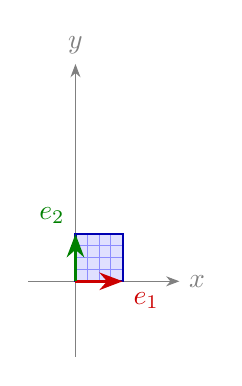
\begin{tikzpicture}[x=0.6cm, y=0.6cm, >=Stealth, baseline=(current bounding box.center)]
        \draw[->, gray] (-1,0) -- (2.2,0) node[right] {$x$};
        \draw[->, gray] (0,-1.6) -- (0,4.6) node[above] {$y$};
        \fill[blue!12] (0,0) -- (1,0) -- (1,1) -- (0,1) -- cycle;
        \foreach \t in {0.25, 0.5, 0.75} {
            \draw[blue!45] (\t,0) -- (\t,1);
            \draw[blue!45] (0,\t) -- (1,\t);
        }
        \draw[blue!70!black, thick] (0,0) -- (1,0) -- (1,1) -- (0,1) -- cycle;
        \draw[->, very thick, red!80!black] (0,0) -- (1,0) node[below right] {$e_1$};
        \draw[->, very thick, green!50!black] (0,0) -- (0,1) node[above left] {$e_2$};
    \end{tikzpicture}
    \quad $\xrightarrow{\quad T \quad}$ \quad
    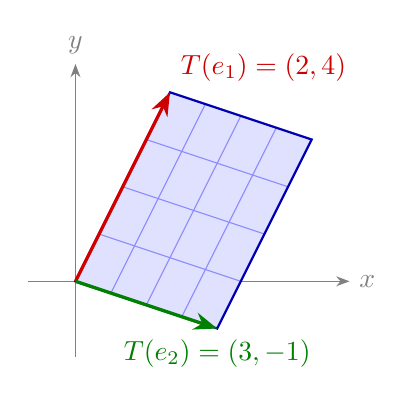
\begin{tikzpicture}[x=0.6cm, y=0.6cm, >=Stealth, baseline=(current bounding box.center)]
        \draw[->, gray] (-1,0) -- (5.8,0) node[right] {$x$};
        \draw[->, gray] (0,-1.6) -- (0,4.6) node[above] {$y$};
        % Unit vectors 0.6 * T(e_1) and 0.6 * T(e_2), so (x, y) is drawn at T(x, y).
        \begin{scope}[x={(1.2cm,2.4cm)}, y={(1.8cm,-0.6cm)}]
            \fill[blue!12] (0,0) -- (1,0) -- (1,1) -- (0,1) -- cycle;
            \foreach \t in {0.25, 0.5, 0.75} {
                \draw[blue!45] (\t,0) -- (\t,1);
                \draw[blue!45] (0,\t) -- (1,\t);
            }
            \draw[blue!70!black, thick] (0,0) -- (1,0) -- (1,1) -- (0,1) -- cycle;
        \end{scope}
        \draw[->, very thick, red!80!black] (0,0) -- (2,4) node[above right] {$T(e_1) = (2, 4)$};
        \draw[->, very thick, green!50!black] (0,0) -- (3,-1) node[below] {$T(e_2) = (3, -1)$};
    \end{tikzpicture}
    \caption[A linear transformation acting on the unit square]{The linear transformation $T(x, y) = (2x + 3y, 4x - y)$ maps the unit square (left) to the parallelogram spanned by $T(e_1)$ and $T(e_2)$ (right). The grid lines inside the square are mapped to equally spaced parallel lines inside the parallelogram.}
    \label{L1-fig:T-grid}
\end{figure}

\begin{figure}[ht]
    \centering
    \gallerypanel{2}{0}{0}{1}{(a) stretch\\ $T(x, y) = (2x, y)$}
    \qquad
    \gallerypanel{0}{1}{-1}{0}{(b) rotation by $90^\circ$\\ $T(x, y) = (-y, x)$}

    \bigskip
    \gallerypanel{1}{0}{0}{-1}{(c) reflection in the $x$-axis\\ $T(x, y) = (x, -y)$}
    \qquad
    \gallerypanel{1}{0}{1}{1}{(d) shear\\ $T(x, y) = (x + y, y)$}
    \caption[Four linear transformations of the plane]{Four linear transformations of the plane. The dashed square and the gray letter F show the unit square before the transformation; the blue parallelogram and the orange letter F show its image. The red and green arrows are $T(e_1)$ and $T(e_2)$. Note that in (c), the image of the letter F is mirrored.}
    \label{L1-fig:gallery}
\end{figure}

\begin{definition}[Kernel]
    The kernel of a linear transformation $T: V \to W$ is the set of all vectors in $V$ that are mapped to the zero vector in $W$. Formally, the kernel is defined as
    \[\ker(T) = \{v \in V : T(v) = 0_W\},\]
    where $0_W$ is the zero vector in $W$.
\end{definition}

\begin{example}\label{L1-ex:ker1}
    Let $T: \mathbb{R}^2 \to \mathbb{R}^2$ be defined by $T(x, y) = (2x + 3y, 4x - y)$. We will find the kernel of $T$.

    To find the kernel, we need to solve the equation $T(x, y) = (0, 0)$:
    \begin{align*}
        2x + 3y &= 0 \\
        4x - y &= 0
    \end{align*}

    From the second equation, we can express $y$ in terms of $x$: $y = 4x$. Substituting this into the first equation gives:
    \begin{align*}
        2x + 3(4x) &= 0 \\
        2x + 12x &= 0 \\
        14x &= 0 \\
        x &= 0
    \end{align*}

    Substituting $x = 0$ back into $y = 4x$, we find that $y = 0$. Therefore, the only solution is $(0, 0)$.

    Thus, the kernel of $T$ is
    \[\ker(T) = \{(0, 0)\}.\]
\end{example}

\begin{example}\label{L1-ex:ker2}
    Let $T: \mathbb{R}^3 \to \mathbb{R}^2$ be defined by $T(x, y, z) = (x + 2y - z, 3x - y + 4z)$. We will find the kernel of $T$.

    To find the kernel, we need to solve the equation $T(x, y, z) = (0, 0)$:
    \begin{align*}
        x + 2y - z &= 0 \\
        3x - y + 4z &= 0
    \end{align*}

    From the first equation, we can express $z$ in terms of $x$ and $y$: $z = x + 2y$. Substituting this into the second equation gives:
    \begin{align*}
        3x - y + 4(x + 2y) &= 0 \\
        3x - y + 4x + 8y &= 0 \\
        7x + 7y &= 0 \\
        x + y &= 0
    \end{align*}

    From this equation, we can express $y$ in terms of $x$: $y = -x$. Substituting this back into the expression for $z$, we get:
    \[z = x + 2(-x) = x - 2x = -x.\]

    Therefore, any vector in the kernel can be expressed as $(x, -x, -x)$ for some scalar $x$. Thus, the kernel of $T$ is
    \[\ker(T) = \{(x, -x, -x) : x \in \mathbb{R}\}.\]
\end{example}

\begin{definition}[Image]
    The image (or range) of a linear transformation $T: V \to W$ is the set of all vectors in $W$ that can be expressed as $T(v)$ for some vector $v \in V$. Formally, the image is defined as
    \[\im(T) = \{w \in W : w = T(v) \text{ for some } v \in V\}.\]
\end{definition}

\begin{example}\label{L1-ex:im1}
    Let $T: \mathbb{R}^2 \to \mathbb{R}^2$ be defined by $T(x, y) = (2x + 3y, 4x - y)$. We will find the image of $T$.

    To find the image, we need to determine all possible outputs of $T$. We will show that every vector of $\mathbb{R}^2$ is an output. Let $(u, v) \in \mathbb{R}^2$ be arbitrary. We look for $x, y \in \mathbb{R}$ such that $T(x, y) = (u, v)$, i.e.,
    \begin{align*}
        u &= 2x + 3y \\
        v &= 4x - y
    \end{align*}

    We can solve this system of equations for $x$ and $y$ in terms of $u$ and $v$. From the second equation, we can express $y$ in terms of $x$ and $v$: $y = 4x - v$. Substituting this into the first equation gives:
    \begin{align*}
        u &= 2x + 3(4x - v) \\
        u &= 2x + 12x - 3v \\
        u &= 14x - 3v
    \end{align*}

    Solving for $x$, we get:
    \[14x = u + 3v \implies x = \frac{u + 3v}{14}.\]

    Substituting this back into the expression for $y$, we get:
    \[y = 4\left(\frac{u + 3v}{14}\right) - v = \frac{4u + 12v - 14v}{14} = \frac{2u - v}{7}.\]

    Let us check that these values work:
    \begin{align*}
        2x + 3y &= \frac{2u + 6v}{14} + \frac{12u - 6v}{14} = u, \\
        4x - y &= \frac{4u + 12v}{14} - \frac{4u - 2v}{14} = v.
    \end{align*}

    Therefore, for any $(u, v) \in \mathbb{R}^2$, we have found $(x, y) \in \mathbb{R}^2$ such that $T(x, y) = (u, v)$. This means that the image of $T$ is all of $\mathbb{R}^2$, i.e.,
    \[\im(T) = \mathbb{R}^2.\]
\end{example}

\begin{example}\label{L1-ex:im2}
    Let $T: \mathbb{R}^3 \to \mathbb{R}^2$ be defined by $T(x, y, z) = (x + 2y - z, 3x - y + 4z)$. We will find the image of $T$.

    As before, we will show that every vector of $\mathbb{R}^2$ is an output of $T$. Let $(u, v) \in \mathbb{R}^2$ be arbitrary. We look for $x, y, z \in \mathbb{R}$ such that $T(x, y, z) = (u, v)$, i.e.,
    \begin{align*}
        u &= x + 2y - z \\
        v &= 3x - y + 4z
    \end{align*}

    From the first equation, we can express $z$ in terms of $x$, $y$, and $u$: $z = x + 2y - u$. Substituting this into the second equation gives:
    \begin{align*}
        v &= 3x - y + 4(x + 2y - u) \\
        v &= 3x - y + 4x + 8y - 4u \\
        v &= 7x + 7y - 4u
    \end{align*}

    Rearranging gives:
    \[7x + 7y = 4u + v.\]

    For any fixed $(u, v)$, this equation describes a line in the $(x, y)$-plane, and every point $(x, y)$ on this line, together with $z = x + 2y - u$, is a solution. For example, we can take $y = 0$ and $x = \frac{4u + v}{7}$, and then $z = x - u = \frac{v - 3u}{7}$. Let us check:
    \[T\left(\frac{4u + v}{7}, 0, \frac{v - 3u}{7}\right) = \left(\frac{(4u + v) - (v - 3u)}{7}, \frac{3(4u + v) + 4(v - 3u)}{7}\right) = (u, v).\]

    Therefore, for any $(u, v) \in \mathbb{R}^2$, we have found $(x, y, z) \in \mathbb{R}^3$ such that $T(x, y, z) = (u, v)$. This means that the image of $T$ is all of $\mathbb{R}^2$, i.e.,
    \[\im(T) = \mathbb{R}^2.\]
\end{example}

\begin{example}\label{L1-ex:kerim-picture}
    Let $T: \mathbb{R}^2 \to \mathbb{R}^2$ be defined by $T(x, y) = (x + 2y, 2x + 4y)$. This map is linear, and it can be written as
    \[T(x, y) = (x + 2y) \cdot (1, 2).\]
    So $T(x, y) = (0, 0)$ if and only if $x + 2y = 0$, and the kernel of $T$ is the line
    \[\ker(T) = \{(-2t, t) : t \in \mathbb{R}\} = \Span\{(-2, 1)\}.\]
    Every output of $T$ is a multiple of $(1, 2)$, and every multiple $s(1, 2) = T(s, 0)$ is an output, so the image of $T$ is the line
    \[\im(T) = \{(s, 2s) : s \in \mathbb{R}\} = \Span\{(1, 2)\}.\]
    More generally, all points of the line $x + 2y = c$, which is parallel to $\ker(T)$, are mapped to the same point $c\,(1, 2)$. So $T$ squashes the whole plane onto the line $\im(T)$, as shown in Figure~\ref{L1-fig:kernel-image}. In particular, $T$ is neither injective nor surjective.
\end{example}

\begin{figure}[ht]
    \centering
    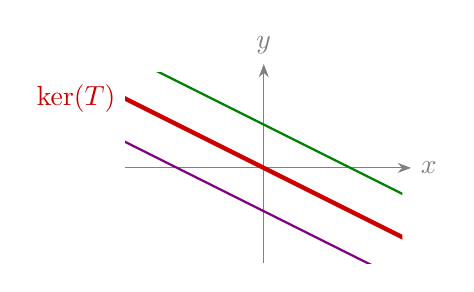
\begin{tikzpicture}[x=0.55cm, y=0.55cm, >=Stealth, baseline=(current bounding box.center)]
        \draw[->, gray] (-3.2,0) -- (3.4,0) node[right] {$x$};
        \draw[->, gray] (0,-2.2) -- (0,2.4) node[above] {$y$};
        \begin{scope}
            \clip (-3.2,-2.2) rectangle (3.2,2.2);
            % The lines x + 2y = c for c = -2, 0, 2, through (c, 0) with direction (-2, 1).
            \draw[thick, violet] (-8,3) -- (4,-3);
            \draw[ultra thick, red!80!black] (-6,3) -- (6,-3);
            \draw[thick, green!50!black] (-4,3) -- (8,-3);
        \end{scope}
        \node[red!80!black, left] at (-3.2,1.6) {$\ker(T)$};
    \end{tikzpicture}
    \quad $\xrightarrow{\quad T \quad}$ \quad
    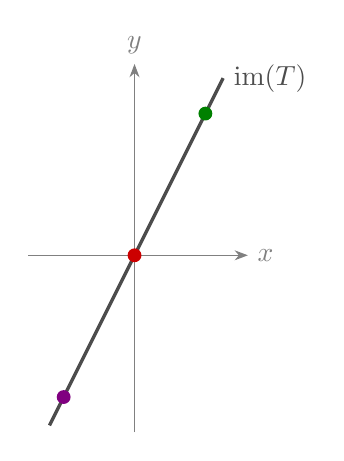
\begin{tikzpicture}[x=0.45cm, y=0.45cm, >=Stealth, baseline=(current bounding box.center)]
        \draw[->, gray] (-3,0) -- (3.2,0) node[right] {$x$};
        \draw[->, gray] (0,-5) -- (0,5.4) node[above] {$y$};
        \draw[very thick, gray!60!black] (-2.4,-4.8) -- (2.5,5) node[right] {$\im(T)$};
        \fill[violet] (-2,-4) circle (2.5pt);
        \fill[red!80!black] (0,0) circle (2.5pt);
        \fill[green!50!black] (2,4) circle (2.5pt);
    \end{tikzpicture}
    \caption[Kernel and image of a linear transformation]{The linear transformation $T(x, y) = (x + 2y, 2x + 4y)$ of Example~\ref{L1-ex:kerim-picture}. Each line $x + 2y = c$ on the left is mapped to the single point $c\,(1, 2)$ on the right, shown in the same color (here $c = -2$, $0$, $2$). The kernel (red, $c = 0$) is mapped to the origin, and the whole plane is squashed onto the line $\im(T)$.}
    \label{L1-fig:kernel-image}
\end{figure}

\subsection{Isomorphisms}

Two vector spaces can look very different and still ``behave in the same way''. For example, a polynomial $a_0 + a_1 x + a_2 x^2$ is added and multiplied by scalars exactly like the list of its coefficients $(a_0, a_1, a_2) \in \mathbb{R}^3$. Isomorphisms make this idea precise.

\begin{definition}[Injective, surjective, bijective]
    A function $f: X \to Y$ between two sets is called
    \begin{itemize}
        \item injective if different inputs give different outputs, i.e., $f(x_1) = f(x_2)$ implies $x_1 = x_2$;
        \item surjective if every element of $Y$ is an output, i.e., for every $y \in Y$ there exists $x \in X$ with $f(x) = y$;
        \item bijective if it is both injective and surjective.
    \end{itemize}
    A function $f$ is bijective if and only if it has an inverse function $f^{-1}: Y \to X$, i.e., a function with $f^{-1}(f(x)) = x$ for all $x \in X$ and $f(f^{-1}(y)) = y$ for all $y \in Y$. Note that a linear transformation $T: V \to W$ is surjective if and only if $\im(T) = W$.
\end{definition}

\begin{definition}[Isomorphism]
    Let $V$ and $W$ be vector spaces over the same field $\mathbb{F}$. An isomorphism from $V$ to $W$ is a bijective linear transformation $T: V \to W$. If there exists an isomorphism from $V$ to $W$, we say that $V$ and $W$ are isomorphic, and we write $V \cong W$.
\end{definition}

\begin{remark}
    An isomorphism $T: V \to W$ matches every vector of $V$ with exactly one vector of $W$, in a way that respects addition and scalar multiplication. So any statement about $V$ that only involves addition and scalar multiplication can be translated into a statement about $W$, and vice versa. In this sense, isomorphic vector spaces are ``the same vector space, written in a different way''.
\end{remark}

To check that a linear transformation is injective, it is enough to look at its kernel.

\begin{lemma}\label{L1-lem:injective}
    A linear transformation $T: V \to W$ is injective if and only if $\ker(T) = \{0_V\}$. Hence $T$ is an isomorphism if and only if $\ker(T) = \{0_V\}$ and $\im(T) = W$.
\end{lemma}

\begin{proof}
    Suppose that $T$ is injective, and let $v \in \ker(T)$. Then $T(v) = 0_W = T(0_V)$ by Lemma~\ref{L1-lem:zero}, so $v = 0_V$.

    Conversely, suppose that $\ker(T) = \{0_V\}$, and let $u, v \in V$ with $T(u) = T(v)$. Using linearity and $(-1) \cdot v = -v$ (Exercise~\ref{L1-ex:axioms}), we get
    \[T(u - v) = T(u + (-1) \cdot v) = T(u) + (-1) \cdot T(v) = T(u) - T(v) = 0_W,\]
    so $u - v \in \ker(T) = \{0_V\}$, i.e., $u = v$.
\end{proof}

\begin{example}\label{L1-ex:iso1}
    The linear transformation $T: \mathbb{R}^2 \to \mathbb{R}^2$, $T(x, y) = (2x + 3y, 4x - y)$, is an isomorphism. Indeed, we found in Example~\ref{L1-ex:ker1} that $\ker(T) = \{(0, 0)\}$, so $T$ is injective by Lemma~\ref{L1-lem:injective}, and we found in Example~\ref{L1-ex:im1} that $\im(T) = \mathbb{R}^2$, so $T$ is surjective. Its inverse is the function we computed in Example~\ref{L1-ex:im1}:
    \[T^{-1}(u, v) = \left(\frac{u + 3v}{14}, \frac{2u - v}{7}\right).\]
\end{example}

\begin{example}
    The linear transformation $T: \mathbb{R}^3 \to \mathbb{R}^2$, $T(x, y, z) = (x + 2y - z, 3x - y + 4z)$, is surjective by Example~\ref{L1-ex:im2}. However, it is not injective, since its kernel is the line $\{(x, -x, -x) : x \in \mathbb{R}\} \neq \{0\}$ (Example~\ref{L1-ex:ker2}). So $T$ is not an isomorphism.

    Similarly, the linear transformation $S: \mathbb{R} \to \mathbb{R}^2$, $S(x) = (x, 0)$, is injective, since $\ker(S) = \{0\}$, but it is not surjective, since $(0, 1)$ is not an output. So $S$ is not an isomorphism either.
\end{example}

\begin{example}\label{L1-ex:iso-poly}
    Let $\mathbb{R}[x]_{\leq 2}$ be the set of polynomials of degree at most $2$, with the usual addition of polynomials and multiplication by real numbers; one can check that it is a vector space over $\mathbb{R}$. The map
    \[T: \mathbb{R}[x]_{\leq 2} \to \mathbb{R}^3, \qquad T(a_0 + a_1 x + a_2 x^2) = (a_0, a_1, a_2),\]
    which lists the coefficients of a polynomial, is an isomorphism. It is linear, since adding two polynomials adds their coefficients, and multiplying a polynomial by a scalar multiplies its coefficients by that scalar. It is injective, since its kernel consists only of the zero polynomial, and it is surjective, since every $(a_0, a_1, a_2) \in \mathbb{R}^3$ is the output $T(a_0 + a_1 x + a_2 x^2)$. Hence $\mathbb{R}[x]_{\leq 2} \cong \mathbb{R}^3$: as far as addition and scalar multiplication are concerned, a polynomial of degree at most $2$ is the same thing as the list of its three coefficients.
\end{example}

\begin{example}
    The complex numbers $\mathbb{C}$ also form a vector space over $\mathbb{R}$, if we only allow multiplication by real scalars. The map $T: \mathbb{C} \to \mathbb{R}^2$, $T(a + bi) = (a, b)$, is linear and bijective (check this!), so it is an isomorphism of vector spaces over $\mathbb{R}$, and $\mathbb{C} \cong \mathbb{R}^2$. This is the familiar picture of complex numbers as points in the plane.
\end{example}

\begin{lemma}\label{L1-lem:composition}
    Let $U$, $V$ and $W$ be vector spaces over the same field $\mathbb{F}$.
    \begin{enumerate}
        \item If $T: U \to V$ and $S: V \to W$ are linear transformations, then their composition $S \circ T: U \to W$, defined by $(S \circ T)(u) = S(T(u))$, is a linear transformation. If $S$ and $T$ are isomorphisms, then so is $S \circ T$.
        \item If $T: V \to W$ is an isomorphism, then its inverse function $T^{-1}: W \to V$ is also linear, and hence an isomorphism.
        \item The identity map $\mathrm{id}_V: V \to V$, $\mathrm{id}_V(v) = v$, is an isomorphism.
    \end{enumerate}
\end{lemma}

\begin{proof}
    (1) For $u_1, u_2, u \in U$ and $a \in \mathbb{F}$, we have
    \begin{align*}
        (S \circ T)(u_1 + u_2) &= S(T(u_1) + T(u_2)) = S(T(u_1)) + S(T(u_2)) = (S \circ T)(u_1) + (S \circ T)(u_2), \\
        (S \circ T)(a u) &= S(a T(u)) = a S(T(u)) = a (S \circ T)(u).
    \end{align*}
    If $S$ and $T$ are bijective, then $S \circ T$ is bijective, with inverse function $T^{-1} \circ S^{-1}$.

    (2) Let $w_1, w_2 \in W$ and $a \in \mathbb{F}$, and let $v_1 = T^{-1}(w_1)$ and $v_2 = T^{-1}(w_2)$. Since $T(v_1 + v_2) = T(v_1) + T(v_2) = w_1 + w_2$, applying $T^{-1}$ gives
    \[T^{-1}(w_1 + w_2) = v_1 + v_2 = T^{-1}(w_1) + T^{-1}(w_2).\]
    Similarly, $T(a v_1) = a T(v_1) = a w_1$ gives $T^{-1}(a w_1) = a v_1 = a T^{-1}(w_1)$. Finally, $T^{-1}$ is bijective, with inverse function $T$.

    (3) The identity map is clearly linear and bijective.
\end{proof}

In particular, $V \cong V$; if $V \cong W$, then $W \cong V$; and if $U \cong V$ and $V \cong W$, then $U \cong W$.

\begin{proposition}\label{L1-prop:iso-basis}
    Let $T: V \to W$ be an isomorphism, and let $\{v_1, \ldots, v_n\}$ be a basis of $V$. Then $\{T(v_1), \ldots, T(v_n)\}$ is a basis of $W$. In particular, if $V$ is finite-dimensional and $V \cong W$, then $W$ is also finite-dimensional and $\dim W = \dim V$.
\end{proposition}

\begin{proof}
    Since $T$ is injective, the vectors $T(v_1), \ldots, T(v_n)$ are $n$ different vectors.

    They span $W$: let $w \in W$. Since $T$ is surjective, $w = T(v)$ for some $v \in V$, and we can write $v = a_1 v_1 + \cdots + a_n v_n$. By linearity, $w = T(v) = a_1 T(v_1) + \cdots + a_n T(v_n)$.

    They are linearly independent: if $a_1 T(v_1) + \cdots + a_n T(v_n) = 0_W$, then by linearity $T(a_1 v_1 + \cdots + a_n v_n) = 0_W$, so $a_1 v_1 + \cdots + a_n v_n \in \ker(T) = \{0_V\}$ by Lemma~\ref{L1-lem:injective}. Since $v_1, \ldots, v_n$ are linearly independent, $a_1 = \cdots = a_n = 0$.
\end{proof}

Conversely, every finite-dimensional vector space is isomorphic to some $\mathbb{R}^n$. To see this, we use coordinates. For the rest of this subsection, we work over the field $\mathbb{R}$; everything works in the same way over any field $\mathbb{F}$, with $\mathbb{F}^n$ in place of $\mathbb{R}^n$.

\begin{definition}[Coordinates]\label{L1-def:coordinates}
    Let $V$ be a vector space over $\mathbb{R}$, and let $\mathcal{B} = (v_1, \ldots, v_n)$ be a basis of $V$ whose vectors are listed in a fixed order (an ordered basis). By Proposition~\ref{L1-prop:unique-rep}, every $v \in V$ can be written in exactly one way as $v = a_1 v_1 + \cdots + a_n v_n$. The vector
    \[[v]_{\mathcal{B}} = (a_1, \ldots, a_n) \in \mathbb{R}^n\]
    is called the coordinate vector of $v$ with respect to $\mathcal{B}$, and the map $\varphi_{\mathcal{B}}: V \to \mathbb{R}^n$, $\varphi_{\mathcal{B}}(v) = [v]_{\mathcal{B}}$, is called the coordinate map.
\end{definition}

\begin{theorem}\label{L1-thm:coordinates}
    Let $V$ be a vector space over $\mathbb{R}$ with an ordered basis $\mathcal{B} = (v_1, \ldots, v_n)$. Then the coordinate map $\varphi_{\mathcal{B}}: V \to \mathbb{R}^n$ is an isomorphism. In particular, every $n$-dimensional vector space over $\mathbb{R}$ is isomorphic to $\mathbb{R}^n$.
\end{theorem}

\begin{proof}
    Let $v = a_1 v_1 + \cdots + a_n v_n$ and $w = b_1 v_1 + \cdots + b_n v_n$, and let $c \in \mathbb{R}$. Then
    \[v + w = (a_1 + b_1) v_1 + \cdots + (a_n + b_n) v_n \qquad \text{and} \qquad cv = (c a_1) v_1 + \cdots + (c a_n) v_n,\]
    and by the uniqueness of these expressions, $[v + w]_{\mathcal{B}} = [v]_{\mathcal{B}} + [w]_{\mathcal{B}}$ and $[cv]_{\mathcal{B}} = c\,[v]_{\mathcal{B}}$. So $\varphi_{\mathcal{B}}$ is linear. It is bijective, because the map $\mathbb{R}^n \to V$, $(a_1, \ldots, a_n) \mapsto a_1 v_1 + \cdots + a_n v_n$, is an inverse function of $\varphi_{\mathcal{B}}$, again by the uniqueness of the expressions.
\end{proof}

\begin{example}
    With the ordered basis $\mathcal{B} = (1, x, x^2)$ of $\mathbb{R}[x]_{\leq 2}$, the coordinate map $\varphi_{\mathcal{B}}$ is exactly the isomorphism of Example~\ref{L1-ex:iso-poly}. With a different ordered basis we get different coordinates: for example, with $\mathcal{B}' = (1, 1 + x, x^2)$, the polynomial $p = 2 + 3x + x^2 = (-1) \cdot 1 + 3 \cdot (1 + x) + 1 \cdot x^2$ has $[p]_{\mathcal{B}'} = (-1, 3, 1)$, while $[p]_{\mathcal{B}} = (2, 3, 1)$.
\end{example}

\begin{corollary}\label{L1-cor:iso-dim}
    Two finite-dimensional vector spaces $V$ and $W$ over $\mathbb{R}$ are isomorphic if and only if $\dim V = \dim W$.
\end{corollary}

\begin{proof}
    If $V \cong W$, then $\dim V = \dim W$ by Proposition~\ref{L1-prop:iso-basis}. Conversely, suppose that $\dim V = \dim W = n$, and choose ordered bases $\mathcal{B}$ of $V$ and $\mathcal{C}$ of $W$. By Theorem~\ref{L1-thm:coordinates} and Lemma~\ref{L1-lem:composition}, the map $\varphi_{\mathcal{C}}^{-1} \circ \varphi_{\mathcal{B}}: V \to W$ is an isomorphism.
\end{proof}

\begin{example}
    Since $\dim \mathbb{R}^2 = 2 \neq 3 = \dim \mathbb{R}^3$, the spaces $\mathbb{R}^2$ and $\mathbb{R}^3$ are not isomorphic: there is no bijective linear transformation between them. On the other hand, any two real vector spaces of dimension $3$, such as $\mathbb{R}[x]_{\leq 2}$ and $\mathbb{R}^3$, are isomorphic. Finally, the infinite-dimensional space $\mathbb{R}[x]$ is not isomorphic to any $\mathbb{R}^n$, by Proposition~\ref{L1-prop:iso-basis}.
\end{example}

\section{Subspaces}

\begin{definition}[Subspace]\label{L1-def:subspace}
    A subspace of a vector space $V$ over $\mathbb{F}$ is a subset $U \subseteq V$ that is itself a vector space under the same operations of vector addition and scalar multiplication defined on $V$. In practice, a subset $U \subseteq V$ is a subspace if and only if it satisfies the following three conditions:
    \begin{enumerate}
        \item The zero vector of $V$ is in $U$, i.e., $0_V \in U$.
        \item $U$ is closed under vector addition: For any $u, v \in U$, we have $u + v \in U$.
        \item $U$ is closed under scalar multiplication: For any $a \in \mathbb{F}$ and any $v \in U$, we have $a \cdot v \in U$.
    \end{enumerate}
\end{definition}

\begin{remark}
    Why are these three conditions enough? Conditions 2 and 3 guarantee that adding vectors of $U$ or multiplying them by scalars never leads outside of $U$. The axioms of associativity, commutativity and distributivity, and $1 \cdot v = v$, then hold in $U$ automatically, because they already hold in $V$. Condition 1 provides the additive identity. Finally, the additive inverse of $v \in U$ is $-v = (-1) \cdot v$ (see Exercise~\ref{L1-ex:axioms} in Section~\ref{L1-sec:exercises}), which lies in $U$ by condition 3.
\end{remark}

\begin{example}
    Let $V = \mathbb{R}^3$ and consider the subset $U = \{(x, y, z) \in \mathbb{R}^3 : x + y + z = 0\}$. We will verify that $U$ is a subspace of $V$.

    First, we check that the zero vector is in $U$:
    \[0_V = (0, 0, 0) \in U \text{ since } 0 + 0 + 0 = 0.\]

    Next, we check closure under vector addition. Let $(x_1, y_1, z_1), (x_2, y_2, z_2) \in U$. Then we have:
    \[x_1 + y_1 + z_1 = 0 \qquad \text{and} \qquad x_2 + y_2 + z_2 = 0.\]
    Now consider their sum:
    \[(x_1, y_1, z_1) + (x_2, y_2, z_2) = (x_1 + x_2, y_1 + y_2, z_1 + z_2).\]
    We need to check if this sum is in $U$:
    \[(x_1 + x_2) + (y_1 + y_2) + (z_1 + z_2) = (x_1 + y_1 + z_1) + (x_2 + y_2 + z_2) = 0 + 0 = 0.\]
    Thus, $(x_1 + x_2, y_1 + y_2, z_1 + z_2) \in U$.

    Finally, we check closure under scalar multiplication. Let $a \in \mathbb{R}$ and $(x, y, z) \in U$. Then we have:
    \[x + y + z = 0.\]
    Now consider the scalar multiple:
    \[a \cdot (x, y, z) = (ax, ay, az).\]
    We need to check if this scalar multiple is in $U$:
    \[ax + ay + az = a(x + y + z) = a \cdot 0 = 0.\]
    Thus, $(ax, ay, az) \in U$.

    Therefore, $U$ is a subspace of $\mathbb{R}^3$.
\end{example}

\begin{theorem}\label{L1-thm:kerim}
    Let $T: V \to W$ be a linear transformation. Then the kernel $\ker(T)$ is a subspace of $V$, and the image $\im(T)$ is a subspace of $W$.
\end{theorem}

\begin{proof}
    \textbf{1. Image is a subspace of $W$:}
    \begin{enumerate}
        \item The zero vector of $W$ is in $\im(T)$ since $T(0_V) = 0_W$ by Lemma~\ref{L1-lem:zero}.
        \item Let $w_1, w_2 \in \im(T)$. Then there exist $v_1, v_2 \in V$ such that $T(v_1) = w_1$ and $T(v_2) = w_2$. We have:
        \[w_1 + w_2 = T(v_1) + T(v_2) = T(v_1 + v_2) \in \im(T).\]
        \item Let $a \in \mathbb{F}$ and $w \in \im(T)$. Then there exists $v \in V$ such that $T(v) = w$. We have:
        \[a \cdot w = a \cdot T(v) = T(a \cdot v) \in \im(T).\]
    \end{enumerate}
    Therefore, $\im(T)$ is a subspace of $W$.

    \textbf{2. Kernel is a subspace of $V$:}
    \begin{enumerate}
        \item The zero vector of $V$ is in $\ker(T)$ since $T(0_V) = 0_W$ by Lemma~\ref{L1-lem:zero}.
        \item Let $v_1, v_2 \in \ker(T)$. Then we have:
        \[T(v_1 + v_2) = T(v_1) + T(v_2) = 0_W + 0_W = 0_W,\]
        which implies that $v_1 + v_2 \in \ker(T)$.
        \item Let $a \in \mathbb{F}$ and $v \in \ker(T)$. Then we have:
        \[T(a \cdot v) = a \cdot T(v) = a \cdot 0_W = 0_W,\]
        which implies that $a \cdot v \in \ker(T)$.
    \end{enumerate}
    Therefore, $\ker(T)$ is a subspace of $V$.
\end{proof}

\section{Matrices}

\begin{definition}[Matrix]
    A matrix is a rectangular array of numbers arranged in rows and columns. An $m \times n$ matrix has $m$ rows and $n$ columns, and is typically denoted by a capital letter, such as $A$. The entry in the $i$-th row and $j$-th column of the matrix $A$ is denoted by $A_{ij}$.
\end{definition}

\begin{example}
    Let $A$ be a $2 \times 3$ matrix given by
    \[A = \begin{pmatrix}
        1 & 2 & 3 \\
        4 & 5 & 6
    \end{pmatrix}.\]
    The entry in the first row and second column is $A_{12} = 2$, and the entry in the second row and third column is $A_{23} = 6$.
\end{example}

\begin{definition}[Transpose]
    The transpose of an $m \times n$ matrix $A$ is the $n \times m$ matrix $A^\top$ with entries $(A^\top)_{ij} = A_{ji}$. In other words, the rows of $A$ become the columns of $A^\top$.
\end{definition}

\begin{example}
    For the matrix $A$ from the previous example,
    \[A^\top = \begin{pmatrix}
        1 & 4 \\
        2 & 5 \\
        3 & 6
    \end{pmatrix}.\]
\end{example}

When working with matrices, we write vectors of $\mathbb{R}^n$ as columns, i.e., as $n \times 1$ matrices. To save space, we often write such a column vector as the transpose of a row:
\[x = (x_1, x_2, \ldots, x_n)^\top = \begin{pmatrix}
    x_1 \\
    x_2 \\
    \vdots \\
    x_n
\end{pmatrix}.\]

\begin{definition}[Matrix--vector product]
    Let $A$ be an $m \times n$ matrix and $x = (x_1, \ldots, x_n)^\top \in \mathbb{R}^n$. The product $Ax$ is the vector in $\mathbb{R}^m$ whose $i$-th entry is
    \[(Ax)_i = A_{i1} x_1 + A_{i2} x_2 + \cdots + A_{in} x_n, \qquad i = 1, \ldots, m.\]
    Note that $Ax$ is only defined when the number of columns of $A$ equals the number of entries of $x$.
\end{definition}

\begin{remark}\label{L1-rem:columns}
    If $a_1, a_2, \ldots, a_n \in \mathbb{R}^m$ denote the columns of $A$, then
    \[Ax = x_1 a_1 + x_2 a_2 + \cdots + x_n a_n,\]
    since the $i$-th entry of the right-hand side is $x_1 A_{i1} + x_2 A_{i2} + \cdots + x_n A_{in}$. In words: $Ax$ is the linear combination of the columns of $A$ whose coefficients are the entries of $x$.
\end{remark}

\begin{example}\label{L1-ex:matvec}
    Let $A = \begin{pmatrix} 1 & 2 & 3 \\ 4 & 5 & 6 \end{pmatrix}$ and $x = (1, 0, -1)^\top$. Then
    \[Ax = \begin{pmatrix}
        1 \cdot 1 + 2 \cdot 0 + 3 \cdot (-1) \\
        4 \cdot 1 + 5 \cdot 0 + 6 \cdot (-1)
    \end{pmatrix} = \begin{pmatrix}
        -2 \\
        -2
    \end{pmatrix} = 1 \cdot \begin{pmatrix} 1 \\ 4 \end{pmatrix} + 0 \cdot \begin{pmatrix} 2 \\ 5 \end{pmatrix} + (-1) \cdot \begin{pmatrix} 3 \\ 6 \end{pmatrix}.\]
\end{example}

\begin{remark}
    For any $m \times n$ matrix $A$, the map $x \mapsto Ax$ is a linear transformation $\mathbb{R}^n \to \mathbb{R}^m$. Indeed, for $x, y \in \mathbb{R}^n$ and $c \in \mathbb{R}$,
    \[(A(x + y))_i = \sum_{j=1}^n A_{ij}(x_j + y_j) = \sum_{j=1}^n A_{ij} x_j + \sum_{j=1}^n A_{ij} y_j = (Ax)_i + (Ay)_i,\]
    and similarly $(A(cx))_i = c\,(Ax)_i$. The next theorem shows that, conversely, every linear transformation $\mathbb{R}^n \to \mathbb{R}^m$ is of this form.
\end{remark}

\begin{theorem}\label{L1-thm:matrix}
    Any linear transformation $T: \mathbb{R}^n \to \mathbb{R}^m$ can be represented by an $m \times n$ matrix $A$ such that for any vector $x \in \mathbb{R}^n$, we have
    \[T(x) = Ax.\]
    The $i$-th column of $A$ is the vector $T(e_i)$.
\end{theorem}

\begin{proof}
    Let $T: \mathbb{R}^n \to \mathbb{R}^m$ be a linear transformation. We will construct an $m \times n$ matrix $A$ that represents $T$.

    Let $\{e_1, e_2, \ldots, e_n\}$ be the standard basis for $\mathbb{R}^n$, where $e_i$ is the vector with a $1$ in the $i$-th position and $0$s elsewhere. For each basis vector $e_i$, we compute $T(e_i)$, which is a vector in $\mathbb{R}^m$. Let
    \[T(e_i) = \begin{pmatrix}
        T(e_i)_1 \\
        T(e_i)_2 \\
        \vdots \\
        T(e_i)_m
    \end{pmatrix}.\]

    We define the matrix $A$ as the matrix whose $i$-th column is $T(e_i)$:
    \[A = \begin{pmatrix}
        T(e_1)_1 & T(e_2)_1 & \cdots & T(e_n)_1 \\
        T(e_1)_2 & T(e_2)_2 & \cdots & T(e_n)_2 \\
        \vdots & \vdots & \ddots & \vdots \\
        T(e_1)_m & T(e_2)_m & \cdots & T(e_n)_m
    \end{pmatrix}.\]

    Now, for any vector $x = (x_1, x_2, \ldots, x_n)^\top \in \mathbb{R}^n$, we can express $x$ as a linear combination of the basis vectors:
    \[x = x_1 e_1 + x_2 e_2 + \cdots + x_n e_n.\]

    Applying the linear transformation $T$ to $x$ and using additivity and homogeneity, we have:
    \[T(x) = T(x_1 e_1 + x_2 e_2 + \cdots + x_n e_n) = x_1 T(e_1) + x_2 T(e_2) + \cdots + x_n T(e_n).\]

    By Remark~\ref{L1-rem:columns}, the right-hand side is exactly the linear combination of the columns of $A$ with coefficients $x_1, \ldots, x_n$, that is,
    \[T(x) = A x.\]
    Therefore, we have shown that any linear transformation $T: \mathbb{R}^n \to \mathbb{R}^m$ can be represented by an $m \times n$ matrix $A$ such that $T(x) = Ax$ for all $x \in \mathbb{R}^n$.
\end{proof}

\begin{example}\label{L1-ex:matT}
    Let $T: \mathbb{R}^2 \to \mathbb{R}^2$ be defined by $T(x, y) = (x - y, 2x + 3y)$. We will find the matrix representation of $T$.

    First, we compute $T(e_1)$ and $T(e_2)$, where $e_1 = (1, 0)$ and $e_2 = (0, 1)$ are the standard basis vectors for $\mathbb{R}^2$:
    \begin{align*}
        T(e_1) &= T(1, 0) = (1 - 0, 2 \cdot 1 + 3 \cdot 0) = (1, 2), \\
        T(e_2) &= T(0, 1) = (0 - 1, 2 \cdot 0 + 3 \cdot 1) = (-1, 3).
    \end{align*}

    Now we can construct the matrix $A$ that represents $T$:
    \[A = \begin{pmatrix}
        T(e_1)_1 & T(e_2)_1 \\
        T(e_1)_2 & T(e_2)_2
    \end{pmatrix} = \begin{pmatrix}
        1 & -1 \\
        2 & 3
    \end{pmatrix}.\]

    Therefore, the matrix representation of the linear transformation $T$ is
    \[A = \begin{pmatrix}
        1 & -1 \\
        2 & 3
    \end{pmatrix}.\]
\end{example}

\begin{example}
    Let $T: \mathbb{R}^3 \to \mathbb{R}^2$ be defined by $T(x, y, z) = (x + 2y - z, 3x - y + 4z)$. We will find the matrix representation of $T$.

    First, we compute $T(e_1)$, $T(e_2)$, and $T(e_3)$, where $e_1 = (1, 0, 0)$, $e_2 = (0, 1, 0)$, and $e_3 = (0, 0, 1)$ are the standard basis vectors for $\mathbb{R}^3$:
    \begin{align*}
        T(e_1) &= T(1, 0, 0) = (1 + 2 \cdot 0 - 0, 3 \cdot 1 - 0 + 4 \cdot 0) = (1, 3), \\
        T(e_2) &= T(0, 1, 0) = (0 + 2 \cdot 1 - 0, 3 \cdot 0 - 1 + 4 \cdot 0) = (2, -1), \\
        T(e_3) &= T(0, 0, 1) = (0 + 2 \cdot 0 - 1, 3 \cdot 0 - 0 + 4 \cdot 1) = (-1, 4).
    \end{align*}

    Now we can construct the matrix $A$ that represents $T$:
    \[A = \begin{pmatrix}
        T(e_1)_1 & T(e_2)_1 & T(e_3)_1 \\
        T(e_1)_2 & T(e_2)_2 & T(e_3)_2
    \end{pmatrix} = \begin{pmatrix}
        1 & 2 & -1 \\
        3 & -1 & 4
    \end{pmatrix}.\]

    Therefore, the matrix representation of the linear transformation $T$ is
    \[A = \begin{pmatrix}
        1 & 2 & -1 \\
        3 & -1 & 4
    \end{pmatrix}.\]
\end{example}

\subsection{Matrix operations}

So far, we have used matrices to represent linear transformations. In this subsection, we learn how to add and multiply matrices; inverses of matrices are discussed in Subsection~\ref{L1-subsec:inverse}, after we have developed row reduction. We write $\mathbb{R}^{m \times n}$ for the set of all $m \times n$ matrices with real entries. For $A \in \mathbb{R}^{m \times n}$, we write $T_A: \mathbb{R}^n \to \mathbb{R}^m$ for the linear transformation $T_A(x) = Ax$.

\subsubsection{Matrix addition}

\begin{definition}[Matrix addition and scalar multiplication]
    Let $A$ and $B$ be $m \times n$ matrices and $c \in \mathbb{R}$. The sum $A + B$ and the scalar multiple $cA$ are the $m \times n$ matrices with entries
    \[(A + B)_{ij} = A_{ij} + B_{ij}, \qquad (cA)_{ij} = c A_{ij}.\]
    In other words, matrices are added and multiplied by scalars entry by entry. The sum $A + B$ is only defined when $A$ and $B$ have the same size.
\end{definition}

\begin{example}
    Let
    \[A = \begin{pmatrix}
        1 & 2 & 3 \\
        4 & 5 & 6
    \end{pmatrix}, \qquad B = \begin{pmatrix}
        0 & -1 & 2 \\
        3 & 1 & -2
    \end{pmatrix}.\]
    Then
    \[A + B = \begin{pmatrix}
        1 + 0 & 2 + (-1) & 3 + 2 \\
        4 + 3 & 5 + 1 & 6 + (-2)
    \end{pmatrix} = \begin{pmatrix}
        1 & 1 & 5 \\
        7 & 6 & 4
    \end{pmatrix},\]
    and
    \[2A = \begin{pmatrix}
        2 & 4 & 6 \\
        8 & 10 & 12
    \end{pmatrix}.\]
    On the other hand, $A + A^\top$ is not defined, since $A$ is a $2 \times 3$ matrix and $A^\top$ is a $3 \times 2$ matrix.
\end{example}

\begin{remark}\label{L1-rem:matrix-space}
    With these operations, $\mathbb{R}^{m \times n}$ is a vector space over $\mathbb{R}$. Indeed, an $m \times n$ matrix is just a list of $mn$ real numbers arranged in a rectangle, and the operations are component-wise, exactly as in $\mathbb{R}^{mn}$. The zero vector of this space is the zero matrix $0$, all of whose entries are $0$, and the additive inverse of $A$ is $-A = (-1)A$. We write $A - B = A + (-B)$. Moreover, $\dim \mathbb{R}^{m \times n} = mn$: a basis consists of the $mn$ matrices that have a single entry equal to $1$ and all other entries equal to $0$.
\end{remark}

\begin{remark}
    Matrix addition corresponds to adding linear transformations: for every $x \in \mathbb{R}^n$,
    \[(A + B)x = Ax + Bx, \qquad (cA)x = c(Ax).\]
    Indeed, $((A + B)x)_i = \sum_j (A_{ij} + B_{ij}) x_j = \sum_j A_{ij} x_j + \sum_j B_{ij} x_j = (Ax)_i + (Bx)_i$, and similarly for $cA$.
\end{remark}

\subsubsection{Matrix multiplication}

Let $A$ be an $m \times n$ matrix and $B$ an $n \times p$ matrix. Then $T_B: \mathbb{R}^p \to \mathbb{R}^n$ and $T_A: \mathbb{R}^n \to \mathbb{R}^m$, so we can first apply $T_B$ and then $T_A$. The result is the composition
\[T_A \circ T_B: \mathbb{R}^p \to \mathbb{R}^m, \qquad x \mapsto A(Bx),\]
which is again a linear transformation by Lemma~\ref{L1-lem:composition}. By Theorem~\ref{L1-thm:matrix}, it is represented by an $m \times p$ matrix, whose $j$-th column is $A(Be_j) = Ab_j$, where $b_j = Be_j$ is the $j$-th column of $B$ (Remark~\ref{L1-rem:columns}). The $i$-th entry of $Ab_j$ is $\sum_{k} A_{ik} B_{kj}$. This motivates the following definition.

\begin{definition}[Matrix multiplication]
    Let $A$ be an $m \times n$ matrix and $B$ an $n \times p$ matrix. The product $AB$ is the $m \times p$ matrix with entries
    \[(AB)_{ij} = A_{i1} B_{1j} + A_{i2} B_{2j} + \cdots + A_{in} B_{nj} = \sum_{k=1}^n A_{ik} B_{kj}.\]
    The product $AB$ is only defined when the number of columns of $A$ equals the number of rows of $B$. An $m \times n$ matrix times an $n \times p$ matrix is an $m \times p$ matrix.
\end{definition}

\begin{remark}\label{L1-rem:two-views}
    There are two useful ways to think about the product $AB$:
    \begin{itemize}
        \item Entry by entry: $(AB)_{ij}$ is obtained by multiplying the entries of the $i$-th row of $A$ with the corresponding entries of the $j$-th column of $B$, and adding up the results.
        \item Column by column: the $j$-th column of $AB$ is $Ab_j$, where $b_j$ is the $j$-th column of $B$:
        \[AB = A \begin{pmatrix} b_1 & b_2 & \cdots & b_p \end{pmatrix} = \begin{pmatrix} Ab_1 & Ab_2 & \cdots & Ab_p \end{pmatrix}.\]
        In particular, if $p = 1$, then $B$ is a single column $x$, and $AB$ is the matrix--vector product $Ax$.
    \end{itemize}
\end{remark}

\begin{example}
    Let
    \[A = \begin{pmatrix}
        1 & 2 & 3 \\
        4 & 5 & 6
    \end{pmatrix}, \qquad B = \begin{pmatrix}
        1 & 0 \\
        0 & 1 \\
        -1 & 2
    \end{pmatrix}.\]
    Since $A$ is $2 \times 3$ and $B$ is $3 \times 2$, the product $AB$ is a $2 \times 2$ matrix. For example, its $(1, 1)$ entry is obtained from the first row of $A$ and the first column of $B$:
    \[(AB)_{11} = 1 \cdot 1 + 2 \cdot 0 + 3 \cdot (-1) = -2.\]
    Computing all four entries in the same way, we get
    \[AB = \begin{pmatrix}
        1 \cdot 1 + 2 \cdot 0 + 3 \cdot (-1) & 1 \cdot 0 + 2 \cdot 1 + 3 \cdot 2 \\
        4 \cdot 1 + 5 \cdot 0 + 6 \cdot (-1) & 4 \cdot 0 + 5 \cdot 1 + 6 \cdot 2
    \end{pmatrix} = \begin{pmatrix}
        -2 & 8 \\
        -2 & 17
    \end{pmatrix}.\]
    Note that the first column of $AB$ is $A(1, 0, -1)^\top = (-2, -2)^\top$, which we computed in Example~\ref{L1-ex:matvec}.

    The product $BA$ is also defined, but it is a $3 \times 3$ matrix:
    \[BA = \begin{pmatrix}
        1 & 2 & 3 \\
        4 & 5 & 6 \\
        7 & 8 & 9
    \end{pmatrix}.\]
    In particular, $AB \neq BA$.
\end{example}

\begin{theorem}\label{L1-thm:composition}
    Let $A$ be an $m \times n$ matrix and $B$ an $n \times p$ matrix. Then for every $x \in \mathbb{R}^p$,
    \[(AB)x = A(Bx).\]
    In other words, $AB$ is the matrix of the composition $T_A \circ T_B$: multiplying matrices corresponds to composing linear transformations.
\end{theorem}

\begin{proof}
    This holds by construction, but we can also check it directly. For each $i = 1, \ldots, m$,
    \begin{align*}
        ((AB)x)_i &= \sum_{j=1}^p (AB)_{ij} x_j = \sum_{j=1}^p \sum_{k=1}^n A_{ik} B_{kj} x_j \\
        &= \sum_{k=1}^n A_{ik} \left(\sum_{j=1}^p B_{kj} x_j\right) = \sum_{k=1}^n A_{ik} (Bx)_k = (A(Bx))_i. \qedhere
    \end{align*}
\end{proof}

\begin{example}
    Let $S, T: \mathbb{R}^2 \to \mathbb{R}^2$ be the linear transformations $S(x, y) = (2x + 3y, 4x - y)$ from Example~\ref{L1-ex:ker1} and $T(x, y) = (x - y, 2x + 3y)$ from Example~\ref{L1-ex:matT}. Their matrices are
    \[A_S = \begin{pmatrix}
        2 & 3 \\
        4 & -1
    \end{pmatrix}, \qquad A_T = \begin{pmatrix}
        1 & -1 \\
        2 & 3
    \end{pmatrix}.\]
    Computing the composition directly, we get
    \begin{align*}
        T(S(x, y)) &= T(2x + 3y, 4x - y) \\
        &= \big((2x + 3y) - (4x - y), \ 2(2x + 3y) + 3(4x - y)\big) \\
        &= (-2x + 4y, 16x + 3y).
    \end{align*}
    On the other hand,
    \[A_T A_S = \begin{pmatrix}
        1 \cdot 2 + (-1) \cdot 4 & 1 \cdot 3 + (-1) \cdot (-1) \\
        2 \cdot 2 + 3 \cdot 4 & 2 \cdot 3 + 3 \cdot (-1)
    \end{pmatrix} = \begin{pmatrix}
        -2 & 4 \\
        16 & 3
    \end{pmatrix},\]
    which is exactly the matrix of $T \circ S$, as Theorem~\ref{L1-thm:composition} predicts.
\end{example}

\begin{definition}[Identity matrix]
    The $n \times n$ identity matrix $I_n$ is the matrix with $1$s on the diagonal and $0$s everywhere else:
    \[(I_n)_{ij} = \begin{cases}
        1 & \text{if } i = j, \\
        0 & \text{if } i \neq j,
    \end{cases} \qquad I_n = \begin{pmatrix}
        1 & 0 & \cdots & 0 \\
        0 & 1 & \cdots & 0 \\
        \vdots & \vdots & \ddots & \vdots \\
        0 & 0 & \cdots & 1
    \end{pmatrix}.\]
    Its columns are the standard basis vectors $e_1, \ldots, e_n$, so $I_n x = x$ for every $x \in \mathbb{R}^n$, i.e., $I_n$ represents the identity map. When the size is clear, we simply write $I$.
\end{definition}

\begin{proposition}\label{L1-prop:mult-props}
    Let $A$, $B$, $C$ be matrices and $c \in \mathbb{R}$. Whenever the sizes are such that the sums and products below are defined, we have:
    \begin{enumerate}
        \item Associativity: $(AB)C = A(BC)$;
        \item Distributivity: $A(B + C) = AB + AC$ and $(A + B)C = AC + BC$;
        \item Scalars: $c(AB) = (cA)B = A(cB)$;
        \item Identity: $I_m A = A = A I_n$ for every $m \times n$ matrix $A$;
        \item Transpose: $(AB)^\top = B^\top A^\top$.
    \end{enumerate}
\end{proposition}

\begin{proof}
    All five properties are checked by comparing entries. For associativity,
    \begin{align*}
        ((AB)C)_{ij} &= \sum_{l} (AB)_{il} C_{lj} = \sum_{l} \sum_{k} A_{ik} B_{kl} C_{lj} \\
        &= \sum_{k} A_{ik} \left(\sum_{l} B_{kl} C_{lj}\right) = \sum_{k} A_{ik} (BC)_{kj} = (A(BC))_{ij}.
    \end{align*}
    For the first distributive law, $(A(B + C))_{ij} = \sum_k A_{ik}(B_{kj} + C_{kj}) = \sum_k A_{ik} B_{kj} + \sum_k A_{ik} C_{kj} = (AB + AC)_{ij}$; the second distributive law and the rule for scalars are checked in the same way. For the identity, $(I_m A)_{ij} = \sum_k (I_m)_{ik} A_{kj} = A_{ij}$, since the only nonzero term is the one with $k = i$; similarly, $A I_n = A$. Finally, for the transpose,
    \[((AB)^\top)_{ij} = (AB)_{ji} = \sum_k A_{jk} B_{ki} = \sum_k (B^\top)_{ik} (A^\top)_{kj} = (B^\top A^\top)_{ij}. \qedhere\]
\end{proof}

\begin{remark}
    Matrix multiplication is not commutative: even when $AB$ and $BA$ are both defined and have the same size, in general $AB \neq BA$. For example,
    \[\begin{pmatrix}
        1 & 1 \\
        0 & 1
    \end{pmatrix} \begin{pmatrix}
        1 & 0 \\
        1 & 1
    \end{pmatrix} = \begin{pmatrix}
        2 & 1 \\
        1 & 1
    \end{pmatrix}, \qquad \begin{pmatrix}
        1 & 0 \\
        1 & 1
    \end{pmatrix} \begin{pmatrix}
        1 & 1 \\
        0 & 1
    \end{pmatrix} = \begin{pmatrix}
        1 & 1 \\
        1 & 2
    \end{pmatrix}.\]
    This matches the fact that composing two linear transformations in a different order usually gives a different result. Another difference from numbers is that a product of two nonzero matrices can be zero:
    \[\begin{pmatrix}
        0 & 1 \\
        0 & 0
    \end{pmatrix} \begin{pmatrix}
        0 & 1 \\
        0 & 0
    \end{pmatrix} = \begin{pmatrix}
        0 & 0 \\
        0 & 0
    \end{pmatrix}.\]
    As a consequence, we cannot ``cancel'' matrices: $AB = AC$ does not imply $B = C$ in general.
\end{remark}

\subsection{Row Reduction}

\begin{definition}[Row echelon form]
    The leading entry (also called the pivot) of a nonzero row of a matrix is its first nonzero entry from the left. A matrix is said to be in row echelon form (REF) if it satisfies the following conditions:
    \begin{enumerate}
        \item All nonzero rows are above any rows of all zeros.
        \item The leading entry of each nonzero row after the first occurs to the right of the leading entry of the previous row.
        \item The leading entry of each nonzero row is $1$.
    \end{enumerate}
\end{definition}

\begin{remark}
    Conditions 1 and 2 imply that all entries below a leading entry are zero. Some textbooks do not require condition 3, i.e., they allow leading entries to be any nonzero numbers. In these notes, we always scale the leading entries to be $1$.
\end{remark}

\begin{example}\label{L1-ex:refA}
    Consider the matrix
    \[A = \begin{pmatrix}
        1 & 2 & 3 \\
        0 & 1 & 4 \\
        0 & 0 & 0
    \end{pmatrix}.\]
    This matrix is in row echelon form because:
    \begin{enumerate}
        \item The nonzero rows are above the row of all zeros.
        \item The leading entry of the second row (in column $2$) is to the right of the leading entry of the first row (in column $1$).
        \item Both leading entries are equal to $1$.
    \end{enumerate}
    Note that nonzero entries above a leading $1$, such as the $2$ in the first row, are allowed.
\end{example}

\begin{example}\label{L1-ex:refB}
    Consider the matrix
    \[B = \begin{pmatrix}
        1 & 0 & 2 \\
        0 & 1 & 3 \\
        0 & 0 & 1
    \end{pmatrix}.\]
    This matrix is also in row echelon form because:
    \begin{enumerate}
        \item There are no rows of all zeros, so the first condition is trivially satisfied.
        \item The leading entry of the second row (in column $2$) is to the right of the leading entry of the first row (in column $1$), and the leading entry of the third row (in column $3$) is to the right of the leading entry of the second row.
        \item All three leading entries are equal to $1$.
    \end{enumerate}
\end{example}

\begin{example}
    Consider the matrix
    \[C = \begin{pmatrix}
        0 & 1 & 2 \\
        0 & 0 & 3 \\
        0 & 0 & 0
    \end{pmatrix}.\]
    This matrix is not in row echelon form because the leading entry of the second row is $3$, not $1$, so the third condition fails. The first two conditions do hold: the row of zeros is at the bottom, and the leading entries are in columns $2$ and $3$, so the leading entry of the second row is to the right of the leading entry of the first row. (A first column consisting of zeros is allowed.) Multiplying the second row by $1/3$ gives a matrix in row echelon form.
\end{example}

\begin{example}
    Consider the matrix
    \[D = \begin{pmatrix}
        1 & 2 & 3 \\
        0 & 0 & 0 \\
        0 & 1 & 4
    \end{pmatrix}.\]
    This matrix is not in row echelon form because the nonzero row (the third row) is below a row of all zeros (the second row). For it to be in row echelon form, all nonzero rows must be above any rows of all zeros.
\end{example}

To transform a matrix into row echelon form, we can use elementary row operations, which include:
\begin{enumerate}
    \item Swapping two rows.
    \item Multiplying a row by a nonzero scalar.
    \item Adding or subtracting a multiple of one row to another row.
\end{enumerate}
Each elementary row operation can be undone by another elementary row operation: we can swap the same two rows again, multiply the same row by the inverse of the scalar, or subtract (add) the same multiple back. Using these operations, every matrix can be brought into row echelon form; this procedure is called Gaussian elimination.

\begin{example}
    Consider the matrix
    \[E = \begin{pmatrix}
        2 & 4 & 6 \\
        1 & 3 & 5 \\
        0 & 0 & 0
    \end{pmatrix}.\]
    We will transform this matrix into row echelon form using elementary row operations.

    First, we swap the first and second rows, so that the first row starts with a $1$:
    \[\begin{pmatrix}
        1 & 3 & 5 \\
        2 & 4 & 6 \\
        0 & 0 & 0
    \end{pmatrix}.\]

    Next, we can eliminate the leading entry in the second row by subtracting $2$ times the first row from the second row:
    \[\begin{pmatrix}
        1 & 3 & 5 \\
        0 & -2 & -4 \\
        0 & 0 & 0
    \end{pmatrix}.\]

    Finally, we can multiply the second row by $-1/2$ to make the leading entry of the second row equal to $1$:
    \[\begin{pmatrix}
        1 & 3 & 5 \\
        0 & 1 & 2 \\
        0 & 0 & 0
    \end{pmatrix}.\]

    The resulting matrix is now in row echelon form.
\end{example}

\begin{example}\label{L1-ex:F}
    Consider the matrix
    \[F = \begin{pmatrix}
        1 & 2 & 3 \\
        4 & 5 & 6 \\
        7 & 8 & 9
    \end{pmatrix}.\]
    We will transform this matrix into row echelon form using elementary row operations.

    First, we can eliminate the leading entry in the second row by subtracting $4$ times the first row from the second row:
    \[\begin{pmatrix}
        1 & 2 & 3 \\
        0 & -3 & -6 \\
        7 & 8 & 9
    \end{pmatrix}.\]

    Next, we can eliminate the leading entry in the third row by subtracting $7$ times the first row from the third row:
    \[\begin{pmatrix}
        1 & 2 & 3 \\
        0 & -3 & -6 \\
        0 & -6 & -12
    \end{pmatrix}.\]

    Now, we can eliminate the leading entry in the third row by subtracting $2$ times the second row from the third row:
    \[\begin{pmatrix}
        1 & 2 & 3 \\
        0 & -3 & -6 \\
        0 & 0 & 0
    \end{pmatrix}.\]

    Finally, we can multiply the second row by $-1/3$ to make the leading entry of the second row equal to $1$:
    \[\begin{pmatrix}
        1 & 2 & 3 \\
        0 & 1 & 2 \\
        0 & 0 & 0
    \end{pmatrix}.\]

    The resulting matrix is now in row echelon form.
\end{example}

Sometimes it is useful to further simplify a matrix in row echelon form.

\begin{definition}[Reduced row echelon form]
    A matrix is in reduced row echelon form (RREF) if it is in row echelon form and, in addition, each leading $1$ is the only nonzero entry in its column.
\end{definition}

For example, the matrices $A$ and $B$ in Examples~\ref{L1-ex:refA} and~\ref{L1-ex:refB} are in row echelon form, but not in reduced row echelon form, because they have nonzero entries above some of their leading $1$s. Every matrix $A$ can be brought into reduced row echelon form by elementary row operations, and one can show that the result does not depend on which operations we use; we denote it by $\RREF(A)$.

\begin{example}\label{L1-ex:G}
    Consider the matrix
    \[G = \begin{pmatrix}
        1 & 2 & 3 \\
        0 & 1 & 2 \\
        0 & 0 & 0
    \end{pmatrix},\]
    which is the row echelon form of the matrix $F$ that we found in Example~\ref{L1-ex:F}. We will transform this matrix into reduced row echelon form (RREF).

    We can eliminate the entry above the leading $1$ in the second row by subtracting $2$ times the second row from the first row:
    \[\begin{pmatrix}
        1 & 0 & -1 \\
        0 & 1 & 2 \\
        0 & 0 & 0
    \end{pmatrix}.\]

    The resulting matrix is now in reduced row echelon form (RREF).
\end{example}

\begin{example}\label{L1-ex:H}
    Consider the matrix
    \[H = \begin{pmatrix}
        1 & 2 & 3 \\
        0 & 1 & 4 \\
        0 & 0 & 1
    \end{pmatrix}.\]
    We will transform this matrix into reduced row echelon form (RREF).

    First, we can eliminate the entry above the leading $1$ in the third row by subtracting $4$ times the third row from the second row:
    \[\begin{pmatrix}
        1 & 2 & 3 \\
        0 & 1 & 0 \\
        0 & 0 & 1
    \end{pmatrix}.\]

    Next, we can eliminate the entry above the leading $1$ in the second row by subtracting $2$ times the second row from the first row:
    \[\begin{pmatrix}
        1 & 0 & 3 \\
        0 & 1 & 0 \\
        0 & 0 & 1
    \end{pmatrix}.\]

    Finally, we can eliminate the entry above the leading $1$ in the third row by subtracting $3$ times the third row from the first row:
    \[\begin{pmatrix}
        1 & 0 & 0 \\
        0 & 1 & 0 \\
        0 & 0 & 1
    \end{pmatrix}.\]

    The resulting matrix is now in reduced row echelon form (RREF).
\end{example}

\subsection{The Inverse of a Matrix}\label{L1-subsec:inverse}

\subsubsection{Definition and basic properties}

For a nonzero number $a$, dividing by $a$ means multiplying by its inverse $a^{-1}$, the number with $a \cdot a^{-1} = a^{-1} \cdot a = 1$. For square matrices, the role of the number $1$ is played by the identity matrix.

\begin{definition}[Inverse matrix]
    An $n \times n$ matrix $A$ is called invertible if there exists an $n \times n$ matrix $B$ such that
    \[AB = BA = I_n.\]
    Such a matrix $B$ is called an inverse of $A$. A square matrix that is not invertible is called singular. (We only consider inverses of square matrices.)
\end{definition}

\begin{proposition}
    An invertible matrix $A$ has exactly one inverse, which we denote by $A^{-1}$.
\end{proposition}

\begin{proof}
    Suppose that $B$ and $C$ are both inverses of $A$. Then, using associativity,
    \[B = B I_n = B(AC) = (BA)C = I_n C = C. \qedhere\]
\end{proof}

\begin{example}
    Let
    \[A = \begin{pmatrix}
        2 & 1 \\
        1 & 1
    \end{pmatrix}, \qquad B = \begin{pmatrix}
        1 & -1 \\
        -1 & 2
    \end{pmatrix}.\]
    Then
    \[AB = \begin{pmatrix}
        2 \cdot 1 + 1 \cdot (-1) & 2 \cdot (-1) + 1 \cdot 2 \\
        1 \cdot 1 + 1 \cdot (-1) & 1 \cdot (-1) + 1 \cdot 2
    \end{pmatrix} = \begin{pmatrix}
        1 & 0 \\
        0 & 1
    \end{pmatrix},\]
    and in the same way $BA = I_2$. So $A$ is invertible and $A^{-1} = B$.
\end{example}

\begin{remark}\label{L1-rem:inverse-solve}
    If $A$ is invertible, then for every $b \in \mathbb{R}^n$ the equation $Ax = b$ has exactly one solution, namely $x = A^{-1}b$. Indeed, $x = A^{-1}b$ is a solution, since $A(A^{-1}b) = (AA^{-1})b = I_n b = b$; and any solution $x$ satisfies $x = I_n x = (A^{-1}A)x = A^{-1}(Ax) = A^{-1}b$. In particular, the only solution of $Ax = 0$ is $x = 0$. In terms of linear transformations, $T_{A^{-1}}$ is the inverse function of $T_A$: it undoes what $T_A$ does.
\end{remark}

\begin{example}\label{L1-ex:singular}
    Not every nonzero square matrix is invertible. By Remark~\ref{L1-rem:inverse-solve}, if $Ax = 0$ for some $x \neq 0$, then $A$ is not invertible. For example, the matrix
    \[A = \begin{pmatrix}
        1 & 2 \\
        2 & 4
    \end{pmatrix}\]
    is singular, since $A(2, -1)^\top = (2 - 2, 4 - 4)^\top = (0, 0)^\top$.
\end{example}

To find the inverse of a matrix $A$, we can solve the equation $Ax = y$ for $x$ in terms of $y$.

\begin{proposition}\label{L1-prop:find-inverse}
    Let $A$ and $B$ be $n \times n$ matrices. Suppose that for every $y \in \mathbb{R}^n$, the equation $Ax = y$ has exactly one solution, and that this solution is $x = By$. Then $A$ is invertible and $A^{-1} = B$.
\end{proposition}

\begin{proof}
    For every $y \in \mathbb{R}^n$, the vector $By$ is a solution of $Ax = y$, so $(AB)y = A(By) = y$. Taking $y = e_j$ shows that the $j$-th column of $AB$ is $e_j$, so $AB = I_n$.

    Now let $x \in \mathbb{R}^n$ and $y = Ax$. Then both $x$ and $By$ are solutions of the equation $Az = y$. Since this equation has exactly one solution, $x = By = (BA)x$. Taking $x = e_j$ shows that the $j$-th column of $BA$ is $e_j$, so $BA = I_n$.
\end{proof}

\begin{example}\label{L1-ex:inverse2x2}
    Let
    \[A = \begin{pmatrix}
        2 & 3 \\
        4 & -1
    \end{pmatrix}\]
    be the matrix of the linear transformation $T(x, y) = (2x + 3y, 4x - y)$. In Example~\ref{L1-ex:im1}, we solved the equation $T(x, y) = (u, v)$, i.e., $A(x, y)^\top = (u, v)^\top$. Each step of that computation was forced, so the solution is unique, and it is
    \[x = \frac{u + 3v}{14}, \qquad y = \frac{2u - v}{7} = \frac{4u - 2v}{14}.\]
    In matrix form,
    \[\begin{pmatrix}
        x \\
        y
    \end{pmatrix} = \frac{1}{14} \begin{pmatrix}
        1 & 3 \\
        4 & -2
    \end{pmatrix} \begin{pmatrix}
        u \\
        v
    \end{pmatrix}.\]
    By Proposition~\ref{L1-prop:find-inverse},
    \[A^{-1} = \frac{1}{14} \begin{pmatrix}
        1 & 3 \\
        4 & -2
    \end{pmatrix}.\]
    We can double-check this:
    \[A A^{-1} = \frac{1}{14} \begin{pmatrix}
        2 \cdot 1 + 3 \cdot 4 & 2 \cdot 3 + 3 \cdot (-2) \\
        4 \cdot 1 + (-1) \cdot 4 & 4 \cdot 3 + (-1) \cdot (-2)
    \end{pmatrix} = \frac{1}{14} \begin{pmatrix}
        14 & 0 \\
        0 & 14
    \end{pmatrix} = I_2.\]
\end{example}

\begin{proposition}\label{L1-prop:inverse-props}
    Let $A$ and $B$ be invertible $n \times n$ matrices. Then:
    \begin{enumerate}
        \item $A^{-1}$ is invertible and $(A^{-1})^{-1} = A$;
        \item $AB$ is invertible and $(AB)^{-1} = B^{-1} A^{-1}$;
        \item $A^\top$ is invertible and $(A^\top)^{-1} = (A^{-1})^\top$.
    \end{enumerate}
\end{proposition}

\begin{proof}
    (1) The equations $A A^{-1} = A^{-1} A = I_n$ say exactly that $A$ is an inverse of $A^{-1}$.

    (2) Using associativity,
    \[(AB)(B^{-1}A^{-1}) = A(BB^{-1})A^{-1} = A I_n A^{-1} = AA^{-1} = I_n,\]
    and similarly $(B^{-1}A^{-1})(AB) = B^{-1}(A^{-1}A)B = B^{-1}B = I_n$.

    (3) Using $(AB)^\top = B^\top A^\top$ and $I_n^\top = I_n$, we get
    \[A^\top (A^{-1})^\top = (A^{-1}A)^\top = I_n^\top = I_n, \qquad (A^{-1})^\top A^\top = (AA^{-1})^\top = I_n. \qedhere\]
\end{proof}

Note the reversed order in part 2: to undo ``first $T_B$, then $T_A$'', we must first undo $T_A$ and then undo $T_B$. By induction, every product of invertible matrices is invertible, with $(A_1 A_2 \cdots A_k)^{-1} = A_k^{-1} \cdots A_2^{-1} A_1^{-1}$.

\subsubsection{Computing the inverse with row reduction}

For larger matrices, solving $Ax = y$ by hand as in Example~\ref{L1-ex:inverse2x2} quickly becomes tedious. We now use row reduction to give a systematic method for deciding whether a square matrix is invertible and for computing its inverse. The key observation is that elementary row operations can be performed by matrix multiplication.

\begin{definition}[Elementary matrix]
    An elementary matrix is a matrix obtained from an identity matrix $I_m$ by a single elementary row operation.
\end{definition}

\begin{example}
    The following are $3 \times 3$ elementary matrices. They are obtained from $I_3$ by swapping rows $1$ and $2$, by multiplying row $2$ by a scalar $c \neq 0$, and by adding $c$ times row $1$ to row $3$, respectively:
    \[\begin{pmatrix}
        0 & 1 & 0 \\
        1 & 0 & 0 \\
        0 & 0 & 1
    \end{pmatrix}, \qquad \begin{pmatrix}
        1 & 0 & 0 \\
        0 & c & 0 \\
        0 & 0 & 1
    \end{pmatrix}, \qquad \begin{pmatrix}
        1 & 0 & 0 \\
        0 & 1 & 0 \\
        c & 0 & 1
    \end{pmatrix}.\]
    Multiplying a $3 \times 2$ matrix from the left by the last of them gives
    \[\begin{pmatrix}
        1 & 0 & 0 \\
        0 & 1 & 0 \\
        c & 0 & 1
    \end{pmatrix} \begin{pmatrix}
        p_1 & p_2 \\
        q_1 & q_2 \\
        r_1 & r_2
    \end{pmatrix} = \begin{pmatrix}
        p_1 & p_2 \\
        q_1 & q_2 \\
        r_1 + c p_1 & r_2 + c p_2
    \end{pmatrix},\]
    which is exactly the result of adding $c$ times row $1$ to row $3$.
\end{example}

\begin{lemma}\label{L1-lem:elementary}
    Let $E$ be the elementary matrix obtained from $I_m$ by some elementary row operation. Then for every $m \times n$ matrix $A$, the product $EA$ is the matrix obtained from $A$ by the same row operation.
\end{lemma}

\begin{proof}
    By the definition of matrix multiplication, $(EA)_{ij} = \sum_k E_{ik} A_{kj}$, so the $i$-th row of $EA$ is
    \[E_{i1} \cdot (\text{row } 1 \text{ of } A) + E_{i2} \cdot (\text{row } 2 \text{ of } A) + \cdots + E_{im} \cdot (\text{row } m \text{ of } A).\]
    On the other hand, every elementary row operation replaces each row by a linear combination of the old rows, with coefficients that depend only on the operation and not on the matrix. For example, adding $c$ times row $1$ to row $3$ replaces row $3$ by $c \cdot (\text{row } 1) + 1 \cdot (\text{row } 3)$ and keeps all other rows. Say that the operation replaces row $i$ by $c_{i1} \cdot (\text{row } 1) + \cdots + c_{im} \cdot (\text{row } m)$. Applying it to $I_m$, whose $k$-th row is $e_k^\top$, the new $i$-th row is $c_{i1} e_1^\top + \cdots + c_{im} e_m^\top = (c_{i1}, \ldots, c_{im})$. Since this is the $i$-th row of $E$, we get $E_{ik} = c_{ik}$ for all $i, k$. Therefore, the $i$-th row of $EA$ is $c_{i1} \cdot (\text{row } 1 \text{ of } A) + \cdots + c_{im} \cdot (\text{row } m \text{ of } A)$, which is the $i$-th row of the matrix obtained from $A$ by the row operation.
\end{proof}

\begin{lemma}\label{L1-lem:elem-inv}
    Every elementary matrix $E$ is invertible, and $E^{-1}$ is the elementary matrix of the row operation that undoes the operation of $E$.
\end{lemma}

\begin{proof}
    Let $E'$ be the elementary matrix of the row operation that undoes the operation of $E$. The matrix $E$ is obtained from $I_m$ by the operation of $E$, and by Lemma~\ref{L1-lem:elementary}, $E'E$ is obtained from $E$ by undoing this operation. Hence $E'E = I_m$. In the same way, $EE' = I_m$.
\end{proof}

As a consequence, if a matrix $R$ is obtained from $A$ by row operations with elementary matrices $E_1, E_2, \ldots, E_k$ (in this order), then
\[R = BA, \qquad \text{where } B = E_k \cdots E_2 E_1\]
is invertible as a product of invertible matrices (Proposition~\ref{L1-prop:inverse-props}).

\begin{theorem}\label{L1-thm:invertible}
    For an $n \times n$ matrix $A$, the following statements are equivalent:
    \begin{enumerate}
        \item $A$ is invertible;
        \item the only solution of $Ax = 0$ is $x = 0$;
        \item $\RREF(A) = I_n$.
    \end{enumerate}
\end{theorem}

\begin{proof}
    ($1 \Rightarrow 2$) This was shown in Remark~\ref{L1-rem:inverse-solve}.

    ($2 \Rightarrow 3$) Suppose that $R = \RREF(A) \neq I_n$; we will find a nonzero solution of $Ax = 0$. If $R$ had $n$ pivots, then each of its $n$ rows would contain a pivot, and the pivot columns $p_1 < p_2 < \cdots < p_n$ would be $n$ different numbers among $1, \ldots, n$, so $p_i = i$ for every $i$. Since each pivot is a $1$ and is the only nonzero entry in its column, this would mean $R = I_n$. So $R$ has fewer than $n$ pivots, and some column $j$ of $R$ contains no pivot. Set $x_j = 1$, and $x_k = 0$ for every other column $k$ without a pivot. Then the equation given by each nonzero row $i$ of $R$ becomes $x_{p_i} + R_{ij} = 0$, so we set $x_{p_i} = -R_{ij}$. This gives a vector $x \neq 0$ with $Rx = 0$. Writing $R = BA$ with $B$ invertible as above, we get
    \[Ax = B^{-1}(BA)x = B^{-1}(Rx) = B^{-1}0 = 0.\]

    ($3 \Rightarrow 1$) Let $E_1, \ldots, E_k$ be the elementary matrices of the row operations that bring $A$ to its reduced row echelon form $\RREF(A) = I_n$, and let $B = E_k \cdots E_1$. Then $BA = I_n$, and $B$ is invertible. Multiplying from the left by $B^{-1}$ gives $A = B^{-1}$, so $A$ is invertible with $A^{-1} = (B^{-1})^{-1} = B$.
\end{proof}

\begin{corollary}\label{L1-cor:one-sided}
    Let $A$ and $B$ be $n \times n$ matrices with $BA = I_n$. Then $A$ is invertible and $A^{-1} = B$. In particular, also $AB = I_n$.
\end{corollary}

\begin{proof}
    If $Ax = 0$, then $x = I_n x = (BA)x = B(Ax) = B0 = 0$. By Theorem~\ref{L1-thm:invertible}, $A$ is invertible, and
    \[B = B I_n = B(AA^{-1}) = (BA)A^{-1} = I_n A^{-1} = A^{-1}. \qedhere\]
\end{proof}

So, to check that a square matrix $B$ is the inverse of $A$, it is enough to check one of the two equations $BA = I_n$ or $AB = I_n$. (In the second case, apply the corollary with the roles of $A$ and $B$ swapped: then $B$ is invertible with $B^{-1} = A$, and hence $A^{-1} = B$.)

\begin{theorem}[Gauss--Jordan method]\label{L1-thm:gauss-jordan}
    Let $A$ be an $n \times n$ matrix, and row reduce the $n \times 2n$ matrix $(A \mid I_n)$, obtained by writing $I_n$ to the right of $A$.
    \begin{itemize}
        \item If the left block becomes $I_n$, then $A$ is invertible, and the right block is $A^{-1}$:
        \[(A \mid I_n) \quad \longrightarrow \quad (I_n \mid A^{-1}).\]
        \item If a row of zeros appears in the left block, then $A$ is not invertible.
    \end{itemize}
\end{theorem}

\begin{proof}
    Let $E_1, \ldots, E_k$ be the elementary matrices of the row operations we perform, and let $B = E_k \cdots E_1$. By Lemma~\ref{L1-lem:elementary} and the column-by-column description of matrix multiplication (Remark~\ref{L1-rem:two-views}), the result is
    \[B\,(A \mid I_n) = (BA \mid B I_n) = (BA \mid B).\]
    In particular, the left block $BA$ is what we get by applying the same row operations to $A$ alone.

    If $BA = I_n$, then $A$ is invertible and $A^{-1} = B$ by Corollary~\ref{L1-cor:one-sided}, and $B$ is exactly the right block.

    If $BA$ has a row of zeros, then $BA$ is not invertible: for every $n \times n$ matrix $M$, the product $(BA)M$ also has a row of zeros, so it cannot be equal to $I_n$. If $A$ were invertible, then $BA$ would be invertible as a product of invertible matrices. Hence $A$ is not invertible.
\end{proof}

One of the two cases always occurs: if $\RREF(A) \neq I_n$, then, as we saw in the proof of Theorem~\ref{L1-thm:invertible}, $\RREF(A)$ has fewer than $n$ pivots, and hence a row of zeros.

\begin{example}
    Let us compute the inverse of the matrix $A$ from Example~\ref{L1-ex:inverse2x2} with the Gauss--Jordan method. We start with
    \[\left(\begin{array}{cc|cc}
        2 & 3 & 1 & 0 \\
        4 & -1 & 0 & 1
    \end{array}\right).\]

    Subtracting $2$ times the first row from the second row gives
    \[\left(\begin{array}{cc|cc}
        2 & 3 & 1 & 0 \\
        0 & -7 & -2 & 1
    \end{array}\right).\]

    Multiplying the second row by $-1/7$ gives
    \[\left(\begin{array}{cc|cc}
        2 & 3 & 1 & 0 \\
        0 & 1 & \frac{2}{7} & -\frac{1}{7}
    \end{array}\right).\]

    Subtracting $3$ times the second row from the first row gives
    \[\left(\begin{array}{cc|cc}
        2 & 0 & \frac{1}{7} & \frac{3}{7} \\
        0 & 1 & \frac{2}{7} & -\frac{1}{7}
    \end{array}\right).\]

    Finally, multiplying the first row by $1/2$ gives
    \[\left(\begin{array}{cc|cc}
        1 & 0 & \frac{1}{14} & \frac{3}{14} \\
        0 & 1 & \frac{2}{7} & -\frac{1}{7}
    \end{array}\right).\]

    The left block is $I_2$, so
    \[A^{-1} = \begin{pmatrix}
        \frac{1}{14} & \frac{3}{14} \\
        \frac{2}{7} & -\frac{1}{7}
    \end{pmatrix} = \frac{1}{14} \begin{pmatrix}
        1 & 3 \\
        4 & -2
    \end{pmatrix},\]
    as we found in Example~\ref{L1-ex:inverse2x2}.
\end{example}

\begin{example}
    Let us find the inverse of
    \[A = \begin{pmatrix}
        1 & 1 & 0 \\
        0 & 1 & 1 \\
        1 & 1 & 1
    \end{pmatrix}.\]
    We start with
    \[\left(\begin{array}{ccc|ccc}
        1 & 1 & 0 & 1 & 0 & 0 \\
        0 & 1 & 1 & 0 & 1 & 0 \\
        1 & 1 & 1 & 0 & 0 & 1
    \end{array}\right).\]

    Subtracting the first row from the third row gives
    \[\left(\begin{array}{ccc|ccc}
        1 & 1 & 0 & 1 & 0 & 0 \\
        0 & 1 & 1 & 0 & 1 & 0 \\
        0 & 0 & 1 & -1 & 0 & 1
    \end{array}\right).\]
    The left block is now in row echelon form, and we continue to its reduced row echelon form.

    Subtracting the third row from the second row gives
    \[\left(\begin{array}{ccc|ccc}
        1 & 1 & 0 & 1 & 0 & 0 \\
        0 & 1 & 0 & 1 & 1 & -1 \\
        0 & 0 & 1 & -1 & 0 & 1
    \end{array}\right).\]

    Subtracting the second row from the first row gives
    \[\left(\begin{array}{ccc|ccc}
        1 & 0 & 0 & 0 & -1 & 1 \\
        0 & 1 & 0 & 1 & 1 & -1 \\
        0 & 0 & 1 & -1 & 0 & 1
    \end{array}\right).\]

    The left block is $I_3$, so
    \[A^{-1} = \begin{pmatrix}
        0 & -1 & 1 \\
        1 & 1 & -1 \\
        -1 & 0 & 1
    \end{pmatrix}.\]
    By Corollary~\ref{L1-cor:one-sided}, to double-check the answer it is enough to verify that $AA^{-1} = I_3$; try it!
\end{example}

\begin{example}
    Let us apply the Gauss--Jordan method to the singular matrix of Example~\ref{L1-ex:singular}:
    \[\left(\begin{array}{cc|cc}
        1 & 2 & 1 & 0 \\
        2 & 4 & 0 & 1
    \end{array}\right).\]
    Subtracting $2$ times the first row from the second row gives
    \[\left(\begin{array}{cc|cc}
        1 & 2 & 1 & 0 \\
        0 & 0 & -2 & 1
    \end{array}\right).\]
    A row of zeros has appeared in the left block, so the matrix is not invertible, as we already knew.
\end{example}

\begin{remark}\label{L1-rem:solve-practice}
    In practice, if we only want to solve $Ax = b$ for one particular $b$, we do not need $A^{-1}$: it is faster, and numerically more accurate, to row reduce the matrix $(A \mid b)$ directly. If $A$ is invertible, the row operations that turn $A$ into $I_n$ turn $(A \mid b)$ into $(I_n \mid A^{-1}b)$, so the solution can be read off from the last column. This is also what numerical libraries do: for example, in NumPy one uses \py{np.linalg.solve(A, b)} rather than \py{np.linalg.inv(A) @ b}.
\end{remark}

\subsubsection{Invertible matrices and isomorphisms}

In Section~\ref{L1-sec:linear}, we defined isomorphisms of vector spaces. We now show that isomorphisms correspond exactly to invertible matrices. We start with the spaces $\mathbb{R}^n$.

\begin{theorem}\label{L1-thm:TA-iso}
    Let $A$ be an $m \times n$ matrix. The linear transformation $T_A: \mathbb{R}^n \to \mathbb{R}^m$, $T_A(x) = Ax$, is an isomorphism if and only if $m = n$ and $A$ is invertible. In this case, $(T_A)^{-1} = T_{A^{-1}}$.
\end{theorem}

\begin{proof}
    Suppose that $m = n$ and $A$ is invertible. Then $A^{-1}(Ax) = (A^{-1}A)x = x$ for all $x \in \mathbb{R}^n$, and $A(A^{-1}y) = (AA^{-1})y = y$ for all $y \in \mathbb{R}^n$. So $T_{A^{-1}}$ is an inverse function of $T_A$. Hence $T_A$ is bijective, i.e., an isomorphism, and $(T_A)^{-1} = T_{A^{-1}}$.

    Conversely, suppose that $T_A$ is an isomorphism. Then $\mathbb{R}^n \cong \mathbb{R}^m$, so $n = \dim \mathbb{R}^n = \dim \mathbb{R}^m = m$ by Proposition~\ref{L1-prop:iso-basis}. Since $T_A$ is injective, Lemma~\ref{L1-lem:injective} shows that the only solution of $Ax = 0$ is $x = 0$. By Theorem~\ref{L1-thm:invertible}, $A$ is invertible.
\end{proof}

To extend this to arbitrary finite-dimensional vector spaces, we represent linear transformations between them by matrices, using coordinates (Definition~\ref{L1-def:coordinates}). As before, we work over $\mathbb{R}$.

\begin{definition}[Matrix of a linear transformation]
    Let $V$ and $W$ be finite-dimensional vector spaces over $\mathbb{R}$, with ordered bases $\mathcal{B} = (v_1, \ldots, v_n)$ of $V$ and $\mathcal{C} = (w_1, \ldots, w_m)$ of $W$, and let $T: V \to W$ be a linear transformation. The matrix of $T$ with respect to $\mathcal{B}$ and $\mathcal{C}$ is the $m \times n$ matrix $[T]_{\mathcal{C}, \mathcal{B}}$ whose $j$-th column is the coordinate vector $[T(v_j)]_{\mathcal{C}}$, written as a column. We say that this matrix represents $T$.
\end{definition}

\begin{proposition}\label{L1-prop:matrix-coords}
    With the notation above, let $A = [T]_{\mathcal{C}, \mathcal{B}}$. Then
    \[[T(v)]_{\mathcal{C}} = A \, [v]_{\mathcal{B}} \qquad \text{for every } v \in V.\]
    In other words, $\varphi_{\mathcal{C}} \circ T = T_A \circ \varphi_{\mathcal{B}}$.
\end{proposition}

\begin{proof}
    Write $v = x_1 v_1 + \cdots + x_n v_n$, so that $[v]_{\mathcal{B}} = (x_1, \ldots, x_n)^\top$. Using the linearity of $T$ and of the coordinate map $\varphi_{\mathcal{C}}$ (Theorem~\ref{L1-thm:coordinates}), we get
    \[[T(v)]_{\mathcal{C}} = [x_1 T(v_1) + \cdots + x_n T(v_n)]_{\mathcal{C}} = x_1 [T(v_1)]_{\mathcal{C}} + \cdots + x_n [T(v_n)]_{\mathcal{C}}.\]
    Since the columns of $A$ are $[T(v_1)]_{\mathcal{C}}, \ldots, [T(v_n)]_{\mathcal{C}}$, the right-hand side is $A [v]_{\mathcal{B}}$ by Remark~\ref{L1-rem:columns}.
\end{proof}

\begin{remark}
    If $V = \mathbb{R}^n$ and $W = \mathbb{R}^m$ with their standard bases, then every vector is its own coordinate vector, and $[T]_{\mathcal{C}, \mathcal{B}}$ is exactly the matrix of Theorem~\ref{L1-thm:matrix}. With other bases, the same linear transformation is usually represented by a different matrix.
\end{remark}

We can now prove the main result of this subsection.

\begin{theorem}\label{L1-thm:iso-matrix}
    Let $V$ and $W$ be finite-dimensional vector spaces over $\mathbb{R}$, with ordered bases $\mathcal{B}$ of $V$ and $\mathcal{C}$ of $W$.
    \begin{enumerate}
        \item A linear transformation $T: V \to W$ is an isomorphism if and only if the matrix $[T]_{\mathcal{C}, \mathcal{B}}$ that represents it is invertible. In this case, $[T^{-1}]_{\mathcal{B}, \mathcal{C}} = ([T]_{\mathcal{C}, \mathcal{B}})^{-1}$.
        \item Consequently, $V$ and $W$ are isomorphic if and only if there exists a linear transformation $T: V \to W$ that is represented by an invertible matrix.
    \end{enumerate}
\end{theorem}

\begin{proof}
    (1) Let $A = [T]_{\mathcal{C}, \mathcal{B}}$. By Proposition~\ref{L1-prop:matrix-coords}, $\varphi_{\mathcal{C}} \circ T = T_A \circ \varphi_{\mathcal{B}}$. Since the coordinate maps are isomorphisms (Theorem~\ref{L1-thm:coordinates}), we can compose with their inverses to get
    \[T_A = \varphi_{\mathcal{C}} \circ T \circ \varphi_{\mathcal{B}}^{-1} \qquad \text{and} \qquad T = \varphi_{\mathcal{C}}^{-1} \circ T_A \circ \varphi_{\mathcal{B}}.\]
    If $T$ is an isomorphism, then so is $T_A$, as a composition of isomorphisms (Lemma~\ref{L1-lem:composition}), and $A$ is invertible by Theorem~\ref{L1-thm:TA-iso}. Conversely, if $A$ is invertible, then $T_A$ is an isomorphism by Theorem~\ref{L1-thm:TA-iso}, and hence so is $T$, again as a composition of isomorphisms.

    In this case, $T^{-1} = \varphi_{\mathcal{B}}^{-1} \circ (T_A)^{-1} \circ \varphi_{\mathcal{C}} = \varphi_{\mathcal{B}}^{-1} \circ T_{A^{-1}} \circ \varphi_{\mathcal{C}}$, so $[T^{-1}(w)]_{\mathcal{B}} = A^{-1} [w]_{\mathcal{C}}$ for every $w \in W$. Taking for $w$ the $j$-th vector of $\mathcal{C}$, whose coordinate vector is $e_j$, shows that the $j$-th column of $[T^{-1}]_{\mathcal{B}, \mathcal{C}}$ is the $j$-th column of $A^{-1}$.

    (2) If $V \cong W$, choose an isomorphism $T: V \to W$; by part 1, the matrix $[T]_{\mathcal{C}, \mathcal{B}}$ that represents it is invertible. Conversely, if some linear transformation $T: V \to W$ is represented by an invertible matrix, then $T$ is an isomorphism by part 1, so $V \cong W$.
\end{proof}

Since only square matrices can be invertible, Theorem~\ref{L1-thm:iso-matrix} gives another explanation of Corollary~\ref{L1-cor:iso-dim}: isomorphic spaces must have the same dimension.

\begin{example}
    The linear transformation $T(x, y) = (2x + 3y, 4x - y)$ of Example~\ref{L1-ex:iso1} is represented, with respect to the standard bases, by the matrix $A$ of Example~\ref{L1-ex:inverse2x2}. Since $A$ is invertible, $T$ is an isomorphism, and $T^{-1}$ is represented by
    \[A^{-1} = \frac{1}{14} \begin{pmatrix}
        1 & 3 \\
        4 & -2
    \end{pmatrix}, \qquad \text{i.e.,} \qquad T^{-1}(u, v) = \left(\frac{u + 3v}{14}, \frac{4u - 2v}{14}\right),\]
    in agreement with Example~\ref{L1-ex:iso1}.
\end{example}

\begin{example}
    Let $\mathbb{R}[x]_{\leq 1}$ be the vector space of polynomials of degree at most $1$, and consider the linear transformation
    \[T: \mathbb{R}[x]_{\leq 1} \to \mathbb{R}^2, \qquad T(p) = (p(0), p(1)),\]
    which evaluates a polynomial at $0$ and at $1$. We use the ordered basis $\mathcal{B} = (1, x)$ of $\mathbb{R}[x]_{\leq 1}$ and the standard basis $\mathcal{C} = (e_1, e_2)$ of $\mathbb{R}^2$. Since $T(1) = (1, 1)$ and $T(x) = (0, 1)$,
    \[[T]_{\mathcal{C}, \mathcal{B}} = \begin{pmatrix}
        1 & 0 \\
        1 & 1
    \end{pmatrix}, \qquad \text{with inverse} \qquad ([T]_{\mathcal{C}, \mathcal{B}})^{-1} = \begin{pmatrix}
        1 & 0 \\
        -1 & 1
    \end{pmatrix}.\]
    (Check that the product of these two matrices is $I_2$.) By Theorem~\ref{L1-thm:iso-matrix}, $T$ is an isomorphism: a polynomial of degree at most $1$ is uniquely determined by its values at $0$ and $1$, and every pair of values occurs. The inverse is given by $[T^{-1}(u, v)]_{\mathcal{B}} = (u, v - u)^\top$, i.e.,
    \[T^{-1}(u, v) = u + (v - u)x.\]
    Indeed, this polynomial takes the value $u$ at $0$ and the value $v$ at $1$.
\end{example}

\subsection{Special Types of Matrices}\label{L1-subsec:special}

Some kinds of square matrices appear so often that they have their own names. Recall from Remark~\ref{L1-rem:matrix-space} that the set $\mathbb{R}^{n \times n}$ of all $n \times n$ matrices is a vector space over $\mathbb{R}$. The entries $A_{11}, A_{22}, \ldots, A_{nn}$ of an $n \times n$ matrix $A$ form its (main) diagonal.

\subsubsection{Matrices defined by their entries}

\begin{definition}[Special types of square matrices]
    An $n \times n$ matrix $A$ is called
    \begin{itemize}
        \item diagonal if $A_{ij} = 0$ whenever $i \neq j$, i.e., all entries outside the diagonal are zero. We write $\diag(d_1, \ldots, d_n)$ for the diagonal matrix with diagonal entries $d_1, \ldots, d_n$;
        \item upper triangular if $A_{ij} = 0$ whenever $i > j$, i.e., all entries below the diagonal are zero;
        \item lower triangular if $A_{ij} = 0$ whenever $i < j$, i.e., all entries above the diagonal are zero;
        \item symmetric if $A^\top = A$, i.e., $A_{ij} = A_{ji}$ for all $i, j$;
        \item skew-symmetric if $A^\top = -A$, i.e., $A_{ij} = -A_{ji}$ for all $i, j$.
    \end{itemize}
    We denote the sets of diagonal, upper triangular, lower triangular, symmetric and skew-symmetric $n \times n$ matrices by $\mathcal{D}_n$, $\mathcal{U}_n$, $\mathcal{L}_n$, $\mathrm{Sym}_n$ and $\mathrm{Skew}_n$, respectively.
\end{definition}

\begin{example}
    Here are examples of each type for $n = 3$:
    \[\underbrace{\begin{pmatrix}
        2 & 0 & 0 \\
        0 & -1 & 0 \\
        0 & 0 & 5
    \end{pmatrix}}_{\text{diagonal}}, \qquad \underbrace{\begin{pmatrix}
        1 & 2 & 3 \\
        0 & 4 & 5 \\
        0 & 0 & 6
    \end{pmatrix}}_{\text{upper triangular}}, \qquad \underbrace{\begin{pmatrix}
        1 & 0 & 0 \\
        2 & 3 & 0 \\
        4 & 5 & 6
    \end{pmatrix}}_{\text{lower triangular}},\]
    \[\underbrace{\begin{pmatrix}
        1 & 2 & 3 \\
        2 & 4 & 5 \\
        3 & 5 & 6
    \end{pmatrix}}_{\text{symmetric}}, \qquad \underbrace{\begin{pmatrix}
        0 & 2 & -3 \\
        -2 & 0 & 1 \\
        3 & -1 & 0
    \end{pmatrix}}_{\text{skew-symmetric}}.\]
    The diagonal matrix above is $\diag(2, -1, 5)$. The identity matrix $I_n$ and the zero matrix are diagonal, and every diagonal matrix is upper triangular, lower triangular and symmetric at the same time. The diagonal entries of a skew-symmetric matrix are always zero, since $A_{ii} = -A_{ii}$ forces $A_{ii} = 0$. Finally, every square matrix in row echelon form is upper triangular, since the pivot of row $i$ lies in column $i$ or further to the right.
\end{example}

\begin{example}
    For any $m \times n$ matrix $A$, the $n \times n$ matrix $A^\top A$ is symmetric, since by Proposition~\ref{L1-prop:mult-props},
    \[(A^\top A)^\top = A^\top (A^\top)^\top = A^\top A.\]
    Matrices of this form appear all the time in machine learning, for example in least squares problems and as covariance matrices.
\end{example}

\begin{remark}
    Products of diagonal matrices are easy to compute: the only nonzero term in $(AB)_{ij} = \sum_k A_{ik} B_{kj}$ can occur for $k = i = j$, so
    \[\diag(a_1, \ldots, a_n) \diag(b_1, \ldots, b_n) = \diag(a_1 b_1, \ldots, a_n b_n).\]
    In particular, if all $d_i \neq 0$, then $\diag(d_1, \ldots, d_n)$ is invertible with inverse $\diag(1/d_1, \ldots, 1/d_n)$. On the other hand, the product of two symmetric matrices need not be symmetric:
    \[\begin{pmatrix}
        1 & 0 \\
        0 & 0
    \end{pmatrix} \begin{pmatrix}
        0 & 1 \\
        1 & 0
    \end{pmatrix} = \begin{pmatrix}
        0 & 1 \\
        0 & 0
    \end{pmatrix}.\]
\end{remark}

The following theorem shows that several of these sets are vector spaces in their own right.

\begin{theorem}\label{L1-thm:special-subspaces}
    The sets $\mathcal{D}_n$, $\mathcal{U}_n$ and $\mathrm{Sym}_n$ are subspaces of $\mathbb{R}^{n \times n}$. In particular, each of them is a vector space over $\mathbb{R}$. Moreover, $\dim \mathcal{D}_n = n$.
\end{theorem}

\begin{proof}
    We check the three conditions of Definition~\ref{L1-def:subspace}. Throughout, let $c \in \mathbb{R}$, and recall that $(A + B)_{ij} = A_{ij} + B_{ij}$ and $(cA)_{ij} = cA_{ij}$.

    \textbf{Diagonal matrices.} The zero matrix is diagonal. If $A, B \in \mathcal{D}_n$ and $i \neq j$, then
    \[(A + B)_{ij} = 0 + 0 = 0 \qquad \text{and} \qquad (cA)_{ij} = c \cdot 0 = 0,\]
    so $A + B \in \mathcal{D}_n$ and $cA \in \mathcal{D}_n$.

    \textbf{Upper triangular matrices.} The zero matrix is upper triangular. If $A, B \in \mathcal{U}_n$ and $i > j$, then $(A + B)_{ij} = 0 + 0 = 0$ and $(cA)_{ij} = c \cdot 0 = 0$, so $A + B \in \mathcal{U}_n$ and $cA \in \mathcal{U}_n$.

    \textbf{Symmetric matrices.} First, note that the transpose respects addition and scalar multiplication: $((A + B)^\top)_{ij} = (A + B)_{ji} = A_{ji} + B_{ji} = (A^\top + B^\top)_{ij}$, so $(A + B)^\top = A^\top + B^\top$, and similarly $(cA)^\top = cA^\top$. The zero matrix is symmetric. If $A, B \in \mathrm{Sym}_n$, then
    \[(A + B)^\top = A^\top + B^\top = A + B \qquad \text{and} \qquad (cA)^\top = cA^\top = cA,\]
    so $A + B \in \mathrm{Sym}_n$ and $cA \in \mathrm{Sym}_n$.

    \textbf{Dimension of $\mathcal{D}_n$.} For $1 \leq i, j \leq n$, let $e_{ij}$ denote the $n \times n$ matrix with a $1$ in position $(i, j)$ and $0$s everywhere else. Every diagonal matrix can be written as
    \[\diag(d_1, \ldots, d_n) = d_1 e_{11} + d_2 e_{22} + \cdots + d_n e_{nn},\]
    so $e_{11}, \ldots, e_{nn}$ span $\mathcal{D}_n$. If $d_1 e_{11} + \cdots + d_n e_{nn} = 0$, then $\diag(d_1, \ldots, d_n)$ is the zero matrix, so $d_1 = \cdots = d_n = 0$. Hence $e_{11}, \ldots, e_{nn}$ are linearly independent, they form a basis of $\mathcal{D}_n$, and $\dim \mathcal{D}_n = n$.
\end{proof}

\begin{exercise}\label{L1-exer:special}
    \begin{enumerate}
        \item Show that $\mathcal{L}_n$ and $\mathrm{Skew}_n$ are subspaces of $\mathbb{R}^{n \times n}$.
        \item Show that $\dim \mathcal{U}_n = \dim \mathcal{L}_n = \dim \mathrm{Sym}_n = \frac{n(n+1)}{2}$ and that $\dim \mathrm{Skew}_n = \frac{n(n-1)}{2}$. (Hint: use the matrices $e_{ij}$.)
        \item Show that the product of two upper triangular matrices is upper triangular.
        \item Show that every $n \times n$ matrix $A$ can be written in exactly one way as $A = S + K$, where $S$ is symmetric and $K$ is skew-symmetric. (Hint: try $S = \frac{1}{2}(A + A^\top)$.)
    \end{enumerate}
\end{exercise}

\subsubsection{Matrix groups}

The next two sets of matrices are defined using multiplication rather than by conditions on the entries, and they behave very differently.

\begin{definition}[General linear group]
    The set of all invertible $n \times n$ matrices is denoted by
    \[\mathrm{GL}(n, \mathbb{R}) = \{A \in \mathbb{R}^{n \times n} : A \text{ is invertible}\}.\]
\end{definition}

\begin{example}
    The identity matrix $I_n$, all elementary matrices (Lemma~\ref{L1-lem:elem-inv}), all diagonal matrices $\diag(d_1, \ldots, d_n)$ with every $d_i \neq 0$, and the matrices of Example~\ref{L1-ex:inverse2x2} belong to $\mathrm{GL}(n, \mathbb{R})$ for the appropriate $n$. The zero matrix and the matrix of Example~\ref{L1-ex:singular} do not.
\end{example}

\begin{proposition}\label{L1-prop:GL}
    The set $\mathrm{GL}(n, \mathbb{R})$ is not a subspace of $\mathbb{R}^{n \times n}$. However, it has the following properties:
    \begin{enumerate}
        \item $I_n \in \mathrm{GL}(n, \mathbb{R})$;
        \item if $A, B \in \mathrm{GL}(n, \mathbb{R})$, then $AB \in \mathrm{GL}(n, \mathbb{R})$;
        \item if $A \in \mathrm{GL}(n, \mathbb{R})$, then $A^{-1} \in \mathrm{GL}(n, \mathbb{R})$.
    \end{enumerate}
\end{proposition}

\begin{proof}
    The zero matrix is not invertible, since $0 \cdot B = 0 \neq I_n$ for every $n \times n$ matrix $B$. So $0 \notin \mathrm{GL}(n, \mathbb{R})$, and the first condition of Definition~\ref{L1-def:subspace} fails. ($\mathrm{GL}(n, \mathbb{R})$ is not closed under addition either: $I_n$ and $-I_n$ are invertible, but $I_n + (-I_n) = 0$ is not.)

    For the three properties: $I_n I_n = I_n$, so $I_n$ is invertible and is its own inverse. Properties 2 and 3 are parts 2 and 1 of Proposition~\ref{L1-prop:inverse-props}.
\end{proof}

\begin{remark}
    A set of matrices that contains $I_n$ and is closed under multiplication and under taking inverses is called a matrix group. This is why $\mathrm{GL}(n, \mathbb{R})$ is called the general linear group. Groups and vector spaces are different kinds of structures: in a vector space we add vectors and multiply them by scalars, while in a group we multiply its elements with each other. Another important matrix group, the special linear group $\mathrm{SL}(n, \mathbb{R})$, is defined using determinants; see Subsection~\ref{L1-subsec:trace-det}.
\end{remark}

\begin{definition}[Orthogonal matrices]
    An $n \times n$ matrix $Q$ is called orthogonal if $Q^\top Q = I_n$. The set of all orthogonal $n \times n$ matrices is denoted by $\mathrm{O}(n)$.
\end{definition}

By Corollary~\ref{L1-cor:one-sided}, every orthogonal matrix $Q$ is invertible with $Q^{-1} = Q^\top$; in particular, also $QQ^\top = I_n$, and $\mathrm{O}(n) \subseteq \mathrm{GL}(n, \mathbb{R})$. So for orthogonal matrices, the inverse comes for free: we only need to transpose.

\begin{example}
    For any angle $\theta$, the rotation matrix
    \[R_\theta = \begin{pmatrix}
        \cos\theta & -\sin\theta \\
        \sin\theta & \cos\theta
    \end{pmatrix}\]
    rotates vectors in the plane counterclockwise by the angle $\theta$. It is orthogonal, since
    \begin{align*}
        R_\theta^\top R_\theta &= \begin{pmatrix}
            \cos\theta & \sin\theta \\
            -\sin\theta & \cos\theta
        \end{pmatrix} \begin{pmatrix}
            \cos\theta & -\sin\theta \\
            \sin\theta & \cos\theta
        \end{pmatrix} \\
        &= \begin{pmatrix}
            \cos^2\theta + \sin^2\theta & -\cos\theta \sin\theta + \sin\theta \cos\theta \\
            -\sin\theta \cos\theta + \cos\theta \sin\theta & \sin^2\theta + \cos^2\theta
        \end{pmatrix} = I_2.
    \end{align*}
    Hence $R_\theta^{-1} = R_\theta^\top = R_{-\theta}$: to undo a rotation by the angle $\theta$, we rotate by $-\theta$.
\end{example}

\begin{example}
    A permutation matrix is a square matrix in which each row and each column contains exactly one $1$, and all other entries are $0$. For example,
    \[P = \begin{pmatrix}
        0 & 1 & 0 \\
        0 & 0 & 1 \\
        1 & 0 & 0
    \end{pmatrix}, \qquad P \begin{pmatrix}
        x_1 \\
        x_2 \\
        x_3
    \end{pmatrix} = \begin{pmatrix}
        x_2 \\
        x_3 \\
        x_1
    \end{pmatrix},\]
    so $P$ permutes the entries of a vector. One checks that $P^\top P = I_3$, so $P$ is orthogonal.
\end{example}

Geometrically, orthogonal matrices are exactly the matrices that preserve lengths and angles, such as rotations, reflections and permutations of the coordinates; we do not prove this here.

\begin{exercise}
    Show that $\mathrm{O}(n)$ is not a subspace of $\mathbb{R}^{n \times n}$, but that it contains $I_n$ and is closed under multiplication and under taking inverses. In other words, $\mathrm{O}(n)$ is a matrix group, called the orthogonal group.
\end{exercise}

\subsection{Trace and Determinant}\label{L1-subsec:trace-det}

In this subsection, we introduce two numbers that can be computed from a square matrix: the trace and the determinant. The trace is very easy to compute, and it depends linearly on the matrix. The determinant is harder to compute, but it tells us whether a matrix is invertible, and it measures how the linear transformation $T_A$ changes areas and volumes.

\subsubsection{The trace}

\begin{definition}[Trace]
    The trace of an $n \times n$ matrix $A$ is the sum of its diagonal entries:
    \[\tr(A) = A_{11} + A_{22} + \cdots + A_{nn} = \sum_{i=1}^n A_{ii}.\]
\end{definition}

\begin{example}
    For the upper triangular matrix from Subsection~\ref{L1-subsec:special},
    \[\tr \begin{pmatrix}
        1 & 2 & 3 \\
        0 & 4 & 5 \\
        0 & 0 & 6
    \end{pmatrix} = 1 + 4 + 6 = 11.\]
    Moreover, $\tr(I_n) = 1 + \cdots + 1 = n$, and the trace of every skew-symmetric matrix is $0$, since its diagonal entries are $0$.
\end{example}

\begin{theorem}\label{L1-thm:trace}
    Let $A$ and $B$ be $n \times n$ matrices and $c \in \mathbb{R}$. Then:
    \begin{enumerate}
        \item $\tr(A + B) = \tr(A) + \tr(B)$ and $\tr(cA) = c \tr(A)$; in other words, $\tr: \mathbb{R}^{n \times n} \to \mathbb{R}$ is a linear transformation;
        \item $\tr(A^\top) = \tr(A)$;
        \item $\tr(AB) = \tr(BA)$. More generally, this holds for every $m \times n$ matrix $A$ and every $n \times m$ matrix $B$.
    \end{enumerate}
\end{theorem}

\begin{proof}
    Parts 1 and 2 follow directly from the definitions, since the diagonal entries of $A + B$, $cA$ and $A^\top$ are $A_{ii} + B_{ii}$, $cA_{ii}$ and $A_{ii}$, respectively. For part 3, let $A$ be an $m \times n$ matrix and $B$ an $n \times m$ matrix. Then
    \begin{align*}
        \tr(AB) &= \sum_{i=1}^m (AB)_{ii} = \sum_{i=1}^m \sum_{k=1}^n A_{ik} B_{ki} \\
        &= \sum_{k=1}^n \sum_{i=1}^m B_{ki} A_{ik} = \sum_{k=1}^n (BA)_{kk} = \tr(BA). \qedhere
    \end{align*}
\end{proof}

\begin{remark}
    Part 3 is surprising, since in general $AB \neq BA$. For example, if $P$ is an invertible $n \times n$ matrix, then
    \[\tr(P^{-1}AP) = \tr\big((P^{-1}A)P\big) = \tr\big(P(P^{-1}A)\big) = \tr(A).\]
    However, the trace is not multiplicative: for
    \[A = \begin{pmatrix}
        1 & 0 \\
        0 & 0
    \end{pmatrix}, \qquad B = \begin{pmatrix}
        0 & 0 \\
        0 & 1
    \end{pmatrix},\]
    we have $AB = 0$, so $\tr(AB) = 0$, while $\tr(A) \tr(B) = 1 \cdot 1 = 1$.
\end{remark}

\begin{example}
    For any $m \times n$ matrix $A$, the diagonal entries of the $n \times n$ matrix $A^\top A$ are
    \[(A^\top A)_{jj} = \sum_{i=1}^m (A^\top)_{ji} A_{ij} = \sum_{i=1}^m A_{ij}^2.\]
    Hence
    \[\tr(A^\top A) = \sum_{i=1}^m \sum_{j=1}^n A_{ij}^2\]
    is the sum of the squares of all entries of $A$. In particular, $\tr(A^\top A) \geq 0$, with equality only for $A = 0$. The number $\|A\|_F = \sqrt{\tr(A^\top A)}$ is called the Frobenius norm of $A$. It is often used in machine learning to measure the size of a matrix, for example of the weight matrix of a layer in a neural network.
\end{example}

\begin{corollary}
    The set $\{A \in \mathbb{R}^{n \times n} : \tr(A) = 0\}$ of matrices with trace zero is a subspace of $\mathbb{R}^{n \times n}$.
\end{corollary}

\begin{proof}
    This set is the kernel of the linear transformation $\tr: \mathbb{R}^{n \times n} \to \mathbb{R}$, so it is a subspace by Theorem~\ref{L1-thm:kerim}.
\end{proof}

\begin{exercise}
    \begin{enumerate}
        \item Show that the subspace of $n \times n$ matrices with trace zero has dimension $n^2 - 1$. (Hint: use the matrices $e_{ij}$ from the proof of Theorem~\ref{L1-thm:special-subspaces}.)
        \item Show that there are no $n \times n$ matrices $A$ and $B$ with $AB - BA = I_n$. (Hint: take the trace of both sides.)
    \end{enumerate}
\end{exercise}

\subsubsection{The determinant}

The determinant of a square matrix is defined recursively: the determinant of an $n \times n$ matrix is expressed in terms of determinants of $(n-1) \times (n-1)$ matrices.

\begin{definition}[Determinant]
    Let $A$ be an $n \times n$ matrix. For $1 \leq i, j \leq n$, let $A^{(ij)}$ denote the $(n-1) \times (n-1)$ matrix obtained from $A$ by deleting its $i$-th row and its $j$-th column. The determinant $\det(A)$ of $A$ is the number defined as follows:
    \begin{itemize}
        \item if $n = 1$, then $\det(A) = A_{11}$;
        \item if $n \geq 2$, then
        \[\det(A) = \sum_{j=1}^n (-1)^{1+j} A_{1j} \det(A^{(1j)}).\]
    \end{itemize}
    Written out, $\det(A) = A_{11} \det(A^{(11)}) - A_{12} \det(A^{(12)}) + A_{13} \det(A^{(13)}) - \cdots$, with alternating signs. This formula is called the cofactor expansion along the first row, and the numbers $C_{ij} = (-1)^{i+j} \det(A^{(ij)})$ are called the cofactors of $A$. The determinant is also denoted by vertical bars, e.g., $\begin{vmatrix} a & b \\ c & d \end{vmatrix} = \det \begin{pmatrix} a & b \\ c & d \end{pmatrix}$.
\end{definition}

\begin{example}[$2 \times 2$ and $3 \times 3$ determinants]
    For a $2 \times 2$ matrix, deleting the first row and the first or the second column leaves the $1 \times 1$ matrices $(d)$ and $(c)$, so
    \[\det \begin{pmatrix}
        a & b \\
        c & d
    \end{pmatrix} = ad - bc.\]
    For a $3 \times 3$ matrix,
    \begin{align*}
        \det \begin{pmatrix}
            a & b & c \\
            d & e & f \\
            g & h & k
        \end{pmatrix} &= a \det \begin{pmatrix}
            e & f \\
            h & k
        \end{pmatrix} - b \det \begin{pmatrix}
            d & f \\
            g & k
        \end{pmatrix} + c \det \begin{pmatrix}
            d & e \\
            g & h
        \end{pmatrix} \\
        &= a(ek - fh) - b(dk - fg) + c(dh - eg).
    \end{align*}
    For example, $\det \begin{pmatrix} 2 & 3 \\ 4 & -1 \end{pmatrix} = 2 \cdot (-1) - 3 \cdot 4 = -14$, and
    \[\det \begin{pmatrix}
        1 & 2 & 3 \\
        4 & 5 & 6 \\
        7 & 8 & 10
    \end{pmatrix} = 1 \cdot (5 \cdot 10 - 6 \cdot 8) - 2 \cdot (4 \cdot 10 - 6 \cdot 7) + 3 \cdot (4 \cdot 8 - 5 \cdot 7) = 2 + 4 - 9 = -3.\]
\end{example}

The following theorem collects the basic properties of the determinant. We state them without proof; they can all be proved by induction on $n$, starting from the definition.

\begin{theorem}\label{L1-thm:det-props}
    Let $A$ be an $n \times n$ matrix.
    \begin{enumerate}
        \item (Expansion along any row or column.) For every row index $i$ and every column index $j$,
        \[\det(A) = \sum_{l=1}^n (-1)^{i+l} A_{il} \det(A^{(il)}) = \sum_{l=1}^n (-1)^{l+j} A_{lj} \det(A^{(lj)}).\]
        \item (Transpose.) $\det(A^\top) = \det(A)$.
        \item (Row operations.)
        \begin{itemize}
            \item Swapping two rows of $A$ multiplies the determinant by $-1$.
            \item Multiplying a row of $A$ by a scalar $c$ multiplies the determinant by $c$.
            \item Adding a multiple of one row to another row does not change the determinant.
        \end{itemize}
    \end{enumerate}
\end{theorem}

By part 2, the same rules hold for the corresponding operations on columns. The signs $(-1)^{i+j}$ in part 1 form a checkerboard pattern, starting with $+$ in the top left corner.

\begin{corollary}\label{L1-cor:det-easy}
    Let $A$ be an $n \times n$ matrix.
    \begin{enumerate}
        \item If $A$ has a row or a column of zeros, then $\det(A) = 0$.
        \item If $A$ has two equal rows, then $\det(A) = 0$.
        \item If $A$ is upper or lower triangular, then $\det(A) = A_{11} A_{22} \cdots A_{nn}$ is the product of its diagonal entries. In particular, $\det(I_n) = 1$.
        \item $\det(cA) = c^n \det(A)$ for every $c \in \mathbb{R}$.
    \end{enumerate}
\end{corollary}

\begin{proof}
    (1) Expand along the row or column of zeros: every term of the sum contains a factor $0$.

    (2) Swapping the two equal rows does not change $A$, but by Theorem~\ref{L1-thm:det-props} it multiplies the determinant by $-1$. So $\det(A) = -\det(A)$, i.e., $\det(A) = 0$.

    (3) Let $A$ be upper triangular. Expanding along the first column, whose only possibly nonzero entry is $A_{11}$, gives $\det(A) = A_{11} \det(A^{(11)})$. The matrix $A^{(11)}$ is again upper triangular, with diagonal entries $A_{22}, \ldots, A_{nn}$, so repeating this argument (formally, by induction on $n$) gives $\det(A) = A_{11} A_{22} \cdots A_{nn}$. If $A$ is lower triangular, then $A^\top$ is upper triangular with the same diagonal, so $\det(A) = \det(A^\top) = A_{11} \cdots A_{nn}$.

    (4) The matrix $cA$ is obtained from $A$ by multiplying each of its $n$ rows by $c$.
\end{proof}

Theorem~\ref{L1-thm:det-props} and Corollary~\ref{L1-cor:det-easy} give an efficient way to compute determinants: bring the matrix into upper triangular form by row operations, keeping track of how each operation changes the determinant, and then multiply the diagonal entries. For large $n$, this is much faster than the cofactor expansion, which involves about $n!$ terms.

\begin{example}
    Let us compute the determinant of the $3 \times 3$ matrix above again, now with row operations. Subtracting $4$ times the first row from the second row, and $7$ times the first row from the third row, does not change the determinant:
    \[\det \begin{pmatrix}
        1 & 2 & 3 \\
        4 & 5 & 6 \\
        7 & 8 & 10
    \end{pmatrix} = \det \begin{pmatrix}
        1 & 2 & 3 \\
        0 & -3 & -6 \\
        0 & -6 & -11
    \end{pmatrix}.\]
    Subtracting $2$ times the second row from the third row does not change it either, and we obtain an upper triangular matrix:
    \[\det \begin{pmatrix}
        1 & 2 & 3 \\
        0 & -3 & -6 \\
        0 & 0 & 1
    \end{pmatrix} = 1 \cdot (-3) \cdot 1 = -3,\]
    in agreement with the cofactor expansion. The matrix $F$ of Example~\ref{L1-ex:F} differs from this matrix only in its bottom right entry, and the same row operations turn it into a matrix with a row of zeros (see Example~\ref{L1-ex:F}). Hence $\det(F) = 0$.
\end{example}

\begin{remark}[Geometric meaning]
    Let $A$ be a $2 \times 2$ matrix. The linear transformation $T_A$ maps the unit square, with sides $e_1$ and $e_2$, to the parallelogram with sides $Ae_1$ and $Ae_2$, which are the columns of $A$. The area of this parallelogram is $|\det(A)|$ (see Figure~\ref{L1-fig:det-area}). More generally, $T_A$ multiplies the area of every region by $|\det(A)|$, and for $3 \times 3$ matrices, $T_A$ multiplies volumes by $|\det(A)|$. The sign of $\det(A)$ tells us whether $T_A$ preserves the orientation (positive sign) or reverses it, like a mirror (negative sign). We do not prove these facts here.

    This picture also makes the rules of Theorem~\ref{L1-thm:det-props} for column operations plausible. Adding a multiple of one column to the other shears the parallelogram, but does not change its base or its height, and hence not its area (see Figure~\ref{L1-fig:det-shear}). Multiplying a column by $c$ stretches the parallelogram by the factor $|c|$ in one direction, which multiplies its area by $|c|$. Swapping the two columns reverses the orientation, which changes the sign of the determinant.
\end{remark}

\begin{figure}[ht]
    \centering
    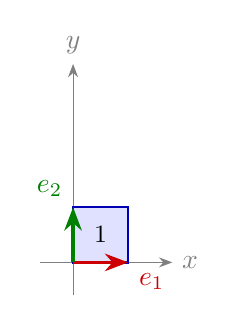
\begin{tikzpicture}[x=0.7cm, y=0.7cm, >=Stealth, baseline=(current bounding box.center)]
        \draw[->, gray] (-0.6,0) -- (1.8,0) node[right] {$x$};
        \draw[->, gray] (0,-0.6) -- (0,3.6) node[above] {$y$};
        \fill[blue!12] (0,0) -- (1,0) -- (1,1) -- (0,1) -- cycle;
        \draw[blue!70!black, thick] (0,0) -- (1,0) -- (1,1) -- (0,1) -- cycle;
        \draw[->, very thick, red!80!black] (0,0) -- (1,0) node[below right] {$e_1$};
        \draw[->, very thick, green!50!black] (0,0) -- (0,1) node[above left] {$e_2$};
        \node[font=\small] at (0.5,0.5) {$1$};
    \end{tikzpicture}
    \quad $\xrightarrow{\quad T_A \quad}$ \quad
    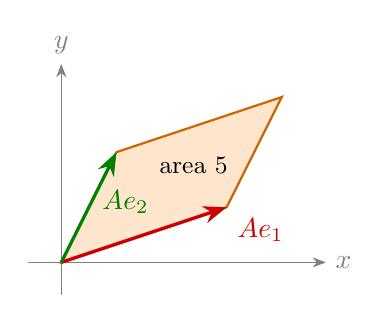
\begin{tikzpicture}[x=0.7cm, y=0.7cm, >=Stealth, baseline=(current bounding box.center)]
        \draw[->, gray] (-0.6,0) -- (4.8,0) node[right] {$x$};
        \draw[->, gray] (0,-0.6) -- (0,3.6) node[above] {$y$};
        \fill[orange!20] (0,0) -- (3,1) -- (4,3) -- (1,2) -- cycle;
        \draw[orange!80!black, thick] (0,0) -- (3,1) -- (4,3) -- (1,2) -- cycle;
        \draw[->, very thick, red!80!black] (0,0) -- (3,1) node[below right] {$Ae_1$};
        \draw[->, very thick, green!50!black] (0,0) -- (1,2) node[pos=0.55, right] {$Ae_2$};
        \node[font=\small] at (2.4,1.75) {area $5$};
    \end{tikzpicture}
    \caption[The determinant as an area]{The matrix $A$ with columns $(3, 1)$ and $(1, 2)$ maps the unit square (left, area $1$) to the parallelogram spanned by its columns $Ae_1$ and $Ae_2$ (right). The area of this parallelogram is $|\det(A)| = |3 \cdot 2 - 1 \cdot 1| = 5$.}
    \label{L1-fig:det-area}
\end{figure}

\begin{figure}[ht]
    \centering
    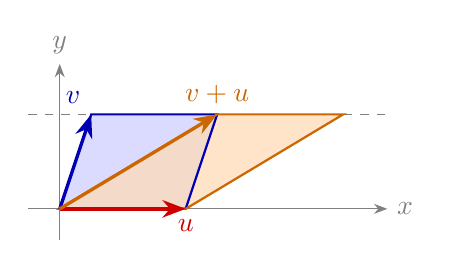
\begin{tikzpicture}[x=0.8cm, y=0.8cm, >=Stealth]
        \draw[->, gray] (-0.5,0) -- (5.2,0) node[right] {$x$};
        \draw[->, gray] (0,-0.5) -- (0,2.3) node[above] {$y$};
        \draw[gray, dashed] (-0.5,1.5) -- (5.2,1.5);
        \fill[blue!20, opacity=0.7] (0,0) -- (2,0) -- (2.5,1.5) -- (0.5,1.5) -- cycle;
        \fill[orange!30, opacity=0.7] (0,0) -- (2,0) -- (4.5,1.5) -- (2.5,1.5) -- cycle;
        \draw[blue!70!black, thick] (0,0) -- (2,0) -- (2.5,1.5) -- (0.5,1.5) -- cycle;
        \draw[orange!80!black, thick] (0,0) -- (2,0) -- (4.5,1.5) -- (2.5,1.5) -- cycle;
        \draw[->, very thick, red!80!black] (0,0) -- (2,0) node[below] {$u$};
        \draw[->, very thick, blue!70!black] (0,0) -- (0.5,1.5) node[above left] {$v$};
        \draw[->, very thick, orange!80!black] (0,0) -- (2.5,1.5) node[above] {$v + u$};
    \end{tikzpicture}
    \caption[Adding one column to another does not change the area]{The parallelograms spanned by $u = (2, 0)$ and $v = (\frac{1}{2}, \frac{3}{2})$ (blue) and by $u$ and $v + u$ (orange) have the same base $u$ and the same height (dashed line), hence the same area $3$. Correspondingly, adding the first column to the second column does not change the determinant: both matrices with these columns have determinant $2 \cdot \frac{3}{2} = 3$.}
    \label{L1-fig:det-shear}
\end{figure}

\begin{example}
    \begin{itemize}
        \item $\det(\diag(2, 3)) = 6$: stretching by a factor $2$ in the $x$-direction and by a factor $3$ in the $y$-direction multiplies areas by $6$.
        \item $\det(R_\theta) = \cos^2\theta + \sin^2\theta = 1$: rotations preserve areas and orientation.
        \item $\det \begin{pmatrix} 1 & 0 \\ 0 & -1 \end{pmatrix} = -1$: the reflection in the $x$-axis preserves areas, but reverses orientation.
        \item $\det \begin{pmatrix} 1 & 2 \\ 2 & 4 \end{pmatrix} = 0$: this singular matrix maps the whole plane onto the line spanned by $(1, 2)$, which has area $0$ (see Figure~\ref{L1-fig:kernel-image}).
    \end{itemize}
    Compare also with the gallery in Figure~\ref{L1-fig:gallery}. The stretch (a) has determinant $\det \begin{pmatrix} 2 & 0 \\ 0 & 1 \end{pmatrix} = 2$ and doubles areas. The rotation (b) and the shear (d) have determinants $\det \begin{pmatrix} 0 & -1 \\ 1 & 0 \end{pmatrix} = 1$ and $\det \begin{pmatrix} 1 & 1 \\ 0 & 1 \end{pmatrix} = 1$: they preserve areas, even though the shear changes the shape of the square. The reflection (c) has determinant $-1$, which is why the image of the letter F is mirrored.
\end{example}

\subsubsection{Determinants, invertibility and products}

We now connect determinants with the inverse of a matrix, using the elementary matrices of Subsection~\ref{L1-subsec:inverse}.

\begin{lemma}\label{L1-lem:det-elementary}
    Let $E$ be an $n \times n$ elementary matrix. Then $\det(E) = -1$ if $E$ swaps two rows, $\det(E) = c$ if $E$ multiplies a row by $c \neq 0$, and $\det(E) = 1$ if $E$ adds a multiple of one row to another row. In all cases, $\det(E) \neq 0$, and
    \[\det(EA) = \det(E) \det(A) \qquad \text{for every } n \times n \text{ matrix } A.\]
\end{lemma}

\begin{proof}
    The matrix $E$ is obtained from $I_n$ by the row operation, and $\det(I_n) = 1$, so the values of $\det(E)$ follow from part 3 of Theorem~\ref{L1-thm:det-props}. By Lemma~\ref{L1-lem:elementary}, $EA$ is obtained from $A$ by the same row operation, so $\det(EA)$ is $\det(A)$ multiplied by $-1$, by $c$, or by $1$, respectively. In each case, this is $\det(E) \det(A)$.
\end{proof}

\begin{theorem}\label{L1-thm:det-invertible}
    An $n \times n$ matrix $A$ is invertible if and only if $\det(A) \neq 0$.
\end{theorem}

\begin{proof}
    Let $E_1, \ldots, E_k$ be the elementary matrices of row operations that bring $A$ to $R = \RREF(A)$, so that $R = E_k \cdots E_1 A$. Applying Lemma~\ref{L1-lem:det-elementary} $k$ times gives
    \[\det(R) = \det(E_k) \cdots \det(E_1) \det(A),\]
    where all the factors $\det(E_i)$ are nonzero. So $\det(A) \neq 0$ if and only if $\det(R) \neq 0$. If $A$ is invertible, then $R = I_n$ by Theorem~\ref{L1-thm:invertible}, and $\det(R) = 1 \neq 0$. If $A$ is not invertible, then $R \neq I_n$, so $R$ has a row of zeros (as we saw after Theorem~\ref{L1-thm:gauss-jordan}), and $\det(R) = 0$ by Corollary~\ref{L1-cor:det-easy}.
\end{proof}

\begin{theorem}[Product rule]\label{L1-thm:det-product}
    For all $n \times n$ matrices $A$ and $B$, we have $\det(AB) = \det(A) \det(B)$.
\end{theorem}

\begin{proof}
    Suppose first that $A$ is not invertible, so that $\det(A) = 0$ by Theorem~\ref{L1-thm:det-invertible}. Then $AB$ is not invertible either: otherwise, $X = B(AB)^{-1}$ would satisfy $AX = I_n$, and by Corollary~\ref{L1-cor:one-sided}, $X$ would be invertible with $X^{-1} = A$, so $A$ would be invertible. Hence $\det(AB) = 0 = \det(A) \det(B)$.

    Now suppose that $A$ is invertible. By the proof of Theorem~\ref{L1-thm:invertible}, $A = (E_k \cdots E_1)^{-1} = E_1^{-1} \cdots E_k^{-1}$ for some elementary matrices $E_1, \ldots, E_k$, and each $F_i = E_i^{-1}$ is again an elementary matrix by Lemma~\ref{L1-lem:elem-inv}. Applying Lemma~\ref{L1-lem:det-elementary} $k$ times, we get
    \[\det(AB) = \det(F_1 F_2 \cdots F_k B) = \det(F_1) \det(F_2) \cdots \det(F_k) \det(B).\]
    Taking $B = I_n$ gives $\det(A) = \det(F_1) \cdots \det(F_k)$, and hence $\det(AB) = \det(A) \det(B)$.
\end{proof}

\begin{corollary}\label{L1-cor:det-consequences}
    Let $A$ be an $n \times n$ matrix.
    \begin{enumerate}
        \item If $A$ is invertible, then $\det(A^{-1}) = 1/\det(A)$.
        \item If $P$ is an invertible $n \times n$ matrix, then $\det(P^{-1}AP) = \det(A)$.
        \item If $A$ is orthogonal, then $\det(A) = 1$ or $\det(A) = -1$.
    \end{enumerate}
\end{corollary}

\begin{proof}
    (1) $\det(A) \det(A^{-1}) = \det(AA^{-1}) = \det(I_n) = 1$.

    (2) $\det(P^{-1}AP) = \det(P^{-1}) \det(A) \det(P) = \det(A)$, by part 1.

    (3) $1 = \det(I_n) = \det(A^\top A) = \det(A^\top) \det(A) = \det(A)^2$.
\end{proof}

\begin{remark}
    Unlike the trace, the determinant is not linear. For example, $\det(I_2 + I_2) = \det(2I_2) = 4$, while $\det(I_2) + \det(I_2) = 2$.
\end{remark}

\begin{example}[Inverse of a $2 \times 2$ matrix]
    Let $A = \begin{pmatrix} a & b \\ c & d \end{pmatrix}$ with $\det(A) = ad - bc \neq 0$. Then
    \[A^{-1} = \frac{1}{ad - bc} \begin{pmatrix}
        d & -b \\
        -c & a
    \end{pmatrix}.\]
    Indeed,
    \[\begin{pmatrix}
        a & b \\
        c & d
    \end{pmatrix} \begin{pmatrix}
        d & -b \\
        -c & a
    \end{pmatrix} = \begin{pmatrix}
        ad - bc & 0 \\
        0 & ad - bc
    \end{pmatrix} = (ad - bc) I_2,\]
    and by Corollary~\ref{L1-cor:one-sided}, checking one product is enough. For example, for the matrix of Example~\ref{L1-ex:inverse2x2}, with determinant $-14$,
    \[\begin{pmatrix}
        2 & 3 \\
        4 & -1
    \end{pmatrix}^{-1} = \frac{1}{-14} \begin{pmatrix}
        -1 & -3 \\
        -4 & 2
    \end{pmatrix} = \frac{1}{14} \begin{pmatrix}
        1 & 3 \\
        4 & -2
    \end{pmatrix},\]
    as we found before. For larger matrices, there is a similar formula, $A^{-1} = \frac{1}{\det(A)} C^\top$, where $C$ is the matrix of cofactors $C_{ij}$; we do not prove it here. For computations, the Gauss--Jordan method is much more efficient.
\end{example}

Theorem~\ref{L1-thm:det-invertible} says that $\mathrm{GL}(n, \mathbb{R}) = \{A \in \mathbb{R}^{n \times n} : \det(A) \neq 0\}$. Determinants also give us another matrix group.

\begin{definition}[Special linear group]
    The special linear group is the set
    \[\mathrm{SL}(n, \mathbb{R}) = \{A \in \mathbb{R}^{n \times n} : \det(A) = 1\}.\]
\end{definition}

\begin{proposition}
    The set $\mathrm{SL}(n, \mathbb{R})$ is contained in $\mathrm{GL}(n, \mathbb{R})$ and is not a subspace of $\mathbb{R}^{n \times n}$. However, it contains $I_n$ and is closed under multiplication and under taking inverses, so it is a matrix group.
\end{proposition}

\begin{proof}
    Every matrix with determinant $1$ is invertible by Theorem~\ref{L1-thm:det-invertible}. The zero matrix has determinant $0$, so it is not in $\mathrm{SL}(n, \mathbb{R})$, and $\mathrm{SL}(n, \mathbb{R})$ is not a subspace. We have $\det(I_n) = 1$. If $\det(A) = \det(B) = 1$, then $\det(AB) = 1 \cdot 1 = 1$ by Theorem~\ref{L1-thm:det-product}, and $\det(A^{-1}) = 1/1 = 1$ by Corollary~\ref{L1-cor:det-consequences}.
\end{proof}

\begin{example}
    All rotation matrices $R_\theta$ belong to $\mathrm{SL}(2, \mathbb{R})$, and so does $\diag(2, \frac{1}{2})$, which stretches the plane by a factor $2$ in one direction and shrinks it by a factor $2$ in the other. By the geometric meaning of the determinant, the matrices in $\mathrm{SL}(2, \mathbb{R})$ are exactly the $2 \times 2$ matrices whose linear transformations preserve areas and orientation.
\end{example}

\section{Null Space, Column Space and Rank}

Row reduction is our main tool for computing the kernel and the image of a linear transformation $T: \mathbb{R}^n \to \mathbb{R}^m$. To use it, we first introduce the corresponding notions for matrices.

\begin{definition}
    Let $A$ be an $m \times n$ matrix.

    The null space of $A$ is the set of all vectors $x \in \mathbb{R}^n$ such that $Ax = 0$. It is denoted as $\Null(A)$. If $T(x) = Ax$, then $\Null(A) = \ker(T)$.

    The column space of $A$ is the set of all linear combinations of the columns of $A$. It is denoted as $\col(A)$. By Remark~\ref{L1-rem:columns}, the vectors $Ax$ are exactly the linear combinations of the columns of $A$, so if $T(x) = Ax$, then $\col(A) = \im(T)$.

    The row space of $A$ is the set of all linear combinations of the rows of $A$. It is denoted as $\row(A)$. Writing the rows as columns, $\row(A) = \col(A^\top)$, which is the image of the linear transformation represented by the transpose $A^\top$.
\end{definition}

By Theorem~\ref{L1-thm:kerim}, $\Null(A)$ is a subspace of $\mathbb{R}^n$ and $\col(A)$ is a subspace of $\mathbb{R}^m$. The following theorem explains how row reduction affects these spaces.

\begin{theorem}\label{L1-thm:rowops}
    Let $A$ be an $m \times n$ matrix, and let $R$ be obtained from $A$ by a sequence of elementary row operations. Then:
    \begin{enumerate}
        \item $\Null(A) = \Null(R)$, i.e., the equations $Ax = 0$ and $Rx = 0$ have exactly the same solutions;
        \item $\row(A) = \row(R)$;
        \item if $R = \RREF(A)$, then the columns of $A$ in the positions of the pivot columns of $R$ (the pivot columns of $A$) form a basis of $\col(A)$.
    \end{enumerate}
\end{theorem}

\begin{proof}
    It is enough to consider a single elementary row operation, since we can then repeat the argument for each operation in the sequence.

    (1) Each equation of the new system is a linear combination of the equations of the old system, so every solution of the old system is also a solution of the new one. Since the operation can be undone by another elementary row operation, the converse holds as well.

    (2) Similarly, every row of the new matrix is a linear combination of the rows of the old matrix, so the new row space is contained in the old one. Undoing the operation shows the reverse inclusion.

    (3) Let $a_1, \ldots, a_n$ be the columns of $A$ and $r_1, \ldots, r_n$ the columns of $R$. For any scalars $c_1, \ldots, c_n$, part (1) applied to $c = (c_1, \ldots, c_n)^\top$ gives
    \[c_1 a_1 + \cdots + c_n a_n = 0 \iff Ac = 0 \iff Rc = 0 \iff c_1 r_1 + \cdots + c_n r_n = 0.\]
    So the columns of $A$ satisfy exactly the same linear relations as the columns of $R$. If $R$ has $r$ pivots, then its pivot columns are the standard basis vectors $e_1, \ldots, e_r$ of $\mathbb{R}^m$, which are linearly independent. Every other column of $R$ has zeros in its last $m - r$ entries, so it is a linear combination of $e_1, \ldots, e_r$. Transferring these relations back to $A$, the pivot columns of $A$ are linearly independent, and every other column of $A$ is a linear combination of them. Hence the pivot columns of $A$ span $\col(A)$, and they form a basis of $\col(A)$.
\end{proof}

\begin{remark}
    Elementary row operations can change the column space! For example,
    \[\begin{pmatrix}
        1 & 1 \\
        1 & 1
    \end{pmatrix} \quad \xrightarrow{\text{subtract row 1 from row 2}} \quad \begin{pmatrix}
        1 & 1 \\
        0 & 0
    \end{pmatrix},\]
    but the column space of the first matrix is $\Span\{(1, 1)^\top\}$, while the column space of the second matrix is $\Span\{(1, 0)^\top\}$. This is why, in part 3 of Theorem~\ref{L1-thm:rowops}, we take the pivot columns of the original matrix $A$, not of $R$.
\end{remark}

\begin{example}\label{L1-ex:worked}
    Consider again the linear transformation $T: \mathbb{R}^3 \to \mathbb{R}^2$ defined by $T(x, y, z) = (x + 2y - z, 3x - y + 4z)$. The matrix representation of $T$ is
    \[A = \begin{pmatrix}
        1 & 2 & -1 \\
        3 & -1 & 4
    \end{pmatrix}.\]

    We will transform this matrix into reduced row echelon form to find the null space, column space and row space of $A$, and hence the kernel and image of $T$.

    First, we can eliminate the leading entry in the second row by subtracting $3$ times the first row from the second row:
    \[\begin{pmatrix}
        1 & 2 & -1 \\
        0 & -7 & 7
    \end{pmatrix}.\]

    Next, we can multiply the second row by $-1/7$ to make the leading entry of the second row equal to $1$:
    \[\begin{pmatrix}
        1 & 2 & -1 \\
        0 & 1 & -1
    \end{pmatrix}.\]

    Now we can eliminate the entry above the leading $1$ in the second row by subtracting $2$ times the second row from the first row:
    \[\RREF(A) = \begin{pmatrix}
        1 & 0 & 1 \\
        0 & 1 & -1
    \end{pmatrix}.\]

    \textbf{Null space.} By Theorem~\ref{L1-thm:rowops}, the equation $Ax = 0$, where $x = (x_1, x_2, x_3)^\top$, has the same solutions as $\RREF(A)\,x = 0$. From the RREF, we have:
    \begin{align*}
        x_1 + x_3 &= 0 \implies x_1 = -x_3, \\
        x_2 - x_3 &= 0 \implies x_2 = x_3.
    \end{align*}

    Letting $x_3 = t$ for some scalar $t$, we have:
    \[x = (-t, t, t)^\top = t(-1, 1, 1)^\top.\]
    Therefore, $\ker(T) = \Null(A) = \Span\{(-1, 1, 1)^\top\}$. This agrees with Example~\ref{L1-ex:ker2}, where we found $\ker(T) = \{(x, -x, -x) : x \in \mathbb{R}\}$ (take $x = -t$).

    \textbf{Column space.} The pivots of $\RREF(A)$ are in columns $1$ and $2$. By Theorem~\ref{L1-thm:rowops}, the first two columns of the original matrix $A$,
    \[\begin{pmatrix}
        1 \\
        3
    \end{pmatrix}, \quad
    \begin{pmatrix}
        2 \\
        -1
    \end{pmatrix},\]
    form a basis of $\col(A)$. These two vectors span all of $\mathbb{R}^2$, since every $(u, v)^\top \in \mathbb{R}^2$ can be written as
    \[\begin{pmatrix}
        u \\
        v
    \end{pmatrix} = \frac{u + 2v}{7} \begin{pmatrix}
        1 \\
        3
    \end{pmatrix} + \frac{3u - v}{7} \begin{pmatrix}
        2 \\
        -1
    \end{pmatrix}.\]
    Hence $\im(T) = \col(A) = \mathbb{R}^2$, which agrees with Example~\ref{L1-ex:im2}.

    \textbf{Row space.} By Theorem~\ref{L1-thm:rowops}, $\row(A) = \row(\RREF(A))$, so the row space of $A$ is spanned by the nonzero rows of the RREF:
    \[\begin{pmatrix}
        1 & 0 & 1
    \end{pmatrix}, \quad
    \begin{pmatrix}
        0 & 1 & -1
    \end{pmatrix}.\]
    These two rows are linearly independent (look at their first two entries), so they form a basis of $\row(A)$.
\end{example}

\begin{definition}[Rank]
    The rank of a matrix $A$ is the dimension of its column space, $\rank(A) = \dim \col(A)$. If $T(x) = Ax$, this is the dimension of the image of $T$.
\end{definition}

\begin{theorem}\label{L1-thm:rank}
    Let $A$ be a matrix, and let $r$ be the number of pivots of $\RREF(A)$, which is the same as the number of nonzero rows of $\RREF(A)$. Then
    \[\rank(A) = r = \dim \row(A).\]
\end{theorem}

\begin{proof}
    By part 3 of Theorem~\ref{L1-thm:rowops}, the $r$ pivot columns of $A$ form a basis of $\col(A)$, so $\rank(A) = r$.

    By part 2 of Theorem~\ref{L1-thm:rowops}, the $r$ nonzero rows of $\RREF(A)$ span $\row(A)$. They are also linearly independent: each of them has a $1$ in its pivot column, where all the other rows have a $0$. So they form a basis of $\row(A)$, and $\dim \row(A) = r$.
\end{proof}

\begin{remark}
    In practice, $\rank(A)$ is the number of nonzero rows in any row echelon form of $A$: clearing the entries above the leading $1$s, as in Examples~\ref{L1-ex:G} and~\ref{L1-ex:H}, turns a row echelon form into the RREF without changing the number of nonzero rows. Also, Theorem~\ref{L1-thm:rank} says that $\dim \col(A) = \dim \row(A)$: a matrix has as many linearly independent columns as linearly independent rows. This is far from obvious!
\end{remark}

\begin{example}
    Consider the matrix
    \[M = \begin{pmatrix}
        1 & 2 & 3 \\
        0 & 1 & 4 \\
        0 & 0 & 0
    \end{pmatrix}.\]
    This matrix is already in row echelon form. The number of nonzero rows is $2$, so the rank of the matrix $M$ is $\rank(M) = 2$. Similarly, the matrix $A$ in Example~\ref{L1-ex:worked} has rank $2$.
\end{example}

\begin{theorem}[Rank--nullity theorem]
    For any $m \times n$ matrix $A$,
    \[\rank(A) + \dim \Null(A) = n.\]
    Equivalently, if $T: \mathbb{R}^n \to \mathbb{R}^m$ is a linear transformation, then $\dim \im(T) + \dim \ker(T) = n$.
\end{theorem}

\begin{proof}[Idea of proof]
    Let $r$ be the number of pivots of $\RREF(A)$, so that $\rank(A) = r$ by Theorem~\ref{L1-thm:rank}. When we solve $\RREF(A)\,x = 0$, the $r$ variables corresponding to the pivot columns are expressed in terms of the remaining $n - r$ free variables. Setting one free variable equal to $1$ and all others equal to $0$ gives $n - r$ solutions. Every solution is a linear combination of these, and they are linearly independent, since each of them has a $1$ in a position where all the others have a $0$. So they form a basis of $\Null(A)$, and $\dim \Null(A) = n - r$.
\end{proof}

\begin{example}
    For $T(x, y, z) = (x + 2y - z, 3x - y + 4z)$, we found in Example~\ref{L1-ex:worked} that $\dim \ker(T) = 1$ and $\dim \im(T) = 2$, and indeed $2 + 1 = 3 = n$. For $T(x, y) = (2x + 3y, 4x - y)$, we found in Examples~\ref{L1-ex:ker1} and~\ref{L1-ex:im1} that $\ker(T) = \{(0, 0)\}$, of dimension $0$, and $\im(T) = \mathbb{R}^2$, of dimension $2$; indeed $2 + 0 = 2 = n$.
\end{example}

Combining the rank--nullity theorem with Theorem~\ref{L1-thm:invertible}, we obtain several ways to recognize an invertible matrix.

\begin{corollary}\label{L1-cor:invertible-rank}
    For an $n \times n$ matrix $A$, the following statements are equivalent:
    \begin{enumerate}
        \item $A$ is invertible;
        \item $\Null(A) = \{0\}$;
        \item $\rank(A) = n$;
        \item for every $b \in \mathbb{R}^n$, the equation $Ax = b$ has exactly one solution;
        \item $\det(A) \neq 0$.
    \end{enumerate}
\end{corollary}

\begin{proof}
    Statements 1 and 2 are equivalent by Theorem~\ref{L1-thm:invertible}. By the rank--nullity theorem, $\rank(A) = n - \dim \Null(A)$, so $\rank(A) = n$ if and only if $\dim \Null(A) = 0$, i.e., $\Null(A) = \{0\}$; hence statements 2 and 3 are equivalent. Statement 1 implies statement 4 by Remark~\ref{L1-rem:inverse-solve}, and statement 4 implies statement 2 by taking $b = 0$. Finally, statements 1 and 5 are equivalent by Theorem~\ref{L1-thm:det-invertible}.
\end{proof}

\begin{exercise}
    Let $T: \mathbb{R}^2 \to \mathbb{R}^2$ be defined by $T(x, y) = (x - y, 2x + 3y)$. Find the kernel and image of $T$, and check that your answer agrees with the rank--nullity theorem.
\end{exercise}

\section{Dual Vector Spaces}\label{L1-sec:dual}

Many important quantities assign a single number to a vector: a coordinate, the average of the entries, the value of a polynomial at a point, the integral of a function, or the prediction $w^\top x$ of a linear model. When such an assignment is linear, it is called a linear functional. The linear functionals on a vector space $V$ form a new vector space, the dual space $V^*$. Duality explains what the transpose of a matrix really is, gives a convenient way to compute coordinates, and provides ``certificates'' showing that a system of linear equations has no solution. In machine learning, the weight vector of a linear model and the derivative of a loss function are naturally elements of a dual space.

Throughout this section, $V$ and $W$ are vector spaces over a field $\mathbb{F}$.

\subsection{Linear functionals and the dual space}

\begin{definition}[Linear functional, dual space]\label{L1-def:dual}
    A linear functional (or linear form) on $V$ is a linear transformation $\varphi: V \to \mathbb{F}$. The set of all linear functionals on $V$ is called the dual space of $V$ and is denoted by $V^*$. For $\varphi, \psi \in V^*$ and $c \in \mathbb{F}$, we define $\varphi + \psi$ and $c\varphi$ pointwise:
    \[(\varphi + \psi)(v) = \varphi(v) + \psi(v), \qquad (c\varphi)(v) = c\, \varphi(v) \qquad (v \in V).\]
\end{definition}

\begin{proposition}
    With these operations, $V^*$ is a vector space over $\mathbb{F}$.
\end{proposition}

\begin{proof}
    The functions $\varphi + \psi$ and $c\varphi$ are again linear; for example, $(\varphi + \psi)(u + v) = \varphi(u) + \varphi(v) + \psi(u) + \psi(v) = (\varphi + \psi)(u) + (\varphi + \psi)(v)$, and similarly for scalar multiples. The vector space axioms hold because they hold pointwise in $\mathbb{F}$, exactly as for the space of all functions $\mathbb{R} \to \mathbb{R}$. The zero vector of $V^*$ is the zero functional $v \mapsto 0$.
\end{proof}

On $\mathbb{R}^n$, the linear functionals are exactly the row vectors.

\begin{proposition}\label{L1-prop:functionals-rn}
    For every row vector $a = (a_1, \ldots, a_n) \in \mathbb{R}^{1 \times n}$, the map $\varphi_a(x) = ax = a_1 x_1 + \cdots + a_n x_n$ is a linear functional on $\mathbb{R}^n$. Conversely, every linear functional $\varphi$ on $\mathbb{R}^n$ is of this form, with $a = \big(\varphi(e_1), \ldots, \varphi(e_n)\big)$. The map $a \mapsto \varphi_a$ is an isomorphism $\mathbb{R}^{1 \times n} \to (\mathbb{R}^n)^*$.
\end{proposition}

\begin{proof}
    The first statement is the case $m = 1$ of matrix--vector multiplication, and the second is the case $m = 1$ of Theorem~\ref{L1-thm:matrix}: the matrix of $\varphi: \mathbb{R}^n \to \mathbb{R}$ is the $1 \times n$ matrix with columns $\varphi(e_1), \ldots, \varphi(e_n)$. The map $a \mapsto \varphi_a$ is linear, since $\varphi_{a + b}(x) = (a + b)x = ax + bx$ and $\varphi_{ca}(x) = c\,ax$; it is surjective by the second statement, and injective since $\varphi_a = 0$ implies $a_i = \varphi_a(e_i) = 0$ for all $i$.
\end{proof}

So vectors of $\mathbb{R}^n$ are columns, and functionals on $\mathbb{R}^n$ are rows; applying a functional to a vector is the product ``row times column''.

\begin{example}\label{L1-ex:functionals}
    The following maps are linear functionals.
    \begin{itemize}
        \item The coordinate functional $x \mapsto x_i$ on $\mathbb{R}^n$, given by the row $e_i^\top$.
        \item The mean $x \mapsto \frac{1}{n}(x_1 + \cdots + x_n)$ on $\mathbb{R}^n$, given by the row $\frac{1}{n}(1, \ldots, 1)$.
        \item The trace $\tr: \mathbb{R}^{n \times n} \to \mathbb{R}$ (Theorem~\ref{L1-thm:trace}).
        \item The evaluation at a point $a$, $\operatorname{ev}_a: \mathbb{R}[x] \to \mathbb{R}$, $p \mapsto p(a)$, and the maps $p \mapsto p'(0)$ and $p \mapsto \int_0^1 p(x)\, dx$.
    \end{itemize}
    On the other hand, $x \mapsto x_1 x_2$, $x \mapsto x_1 + 1$ and $A \mapsto \det(A)$ (for $n \geq 2$) are not linear, so they are not linear functionals.
\end{example}

\begin{remark}[Linear models]
    A linear model in machine learning predicts a number from a feature vector $x \in \mathbb{R}^n$ by $f(x) = w_1 x_1 + \cdots + w_n x_n = w^\top x$. So the model is a linear functional, and learning a linear model means choosing an element of the dual space $(\mathbb{R}^n)^*$. This is one reason why it is natural to write the weights as a row $w^\top$, and the data as columns.
\end{remark}

The kernel of a nonzero linear functional on $\mathbb{R}^n$ is the null space of a nonzero $1 \times n$ matrix $a$, so by the rank--nullity theorem it is a subspace of dimension $n - 1$, called a hyperplane (through the origin). For example, the kernel of $x \mapsto x_1 + x_2 + x_3$ is the plane $x_1 + x_2 + x_3 = 0$ in $\mathbb{R}^3$. Using coordinates, the same holds for every $n$-dimensional vector space.

\subsection{The dual basis}

For indices $i$ and $j$, we use the Kronecker delta
\[\delta_{ij} = \begin{cases} 1 & \text{if } i = j, \\ 0 & \text{if } i \neq j. \end{cases}\]

\begin{theorem}[Dual basis]\label{L1-thm:dual-basis}
    Let $V$ be finite-dimensional with an ordered basis $\mathcal{B} = (b_1, \ldots, b_n)$. For $i = 1, \ldots, n$, let $b^i \in V^*$ be the linear functional that maps a vector to its $i$-th coordinate with respect to $\mathcal{B}$:
    \[b^i(a_1 b_1 + \cdots + a_n b_n) = a_i, \qquad \text{so that} \qquad b^i(b_j) = \delta_{ij}.\]
    Then $(b^1, \ldots, b^n)$ is an ordered basis of $V^*$, called the dual basis of $\mathcal{B}$. Moreover, every $\varphi \in V^*$ can be written as
    \[\varphi = \varphi(b_1)\, b^1 + \varphi(b_2)\, b^2 + \cdots + \varphi(b_n)\, b^n.\]
    In particular, $\dim V^* = \dim V$, so $V^* \cong V$.
\end{theorem}

Here the superscripts in $b^1, \ldots, b^n$ are indices, not powers.

\begin{proof}
    Each $b^i$ is linear, since the coordinate map $v \mapsto [v]_{\mathcal{B}}$ is linear (Theorem~\ref{L1-thm:coordinates}). First, two linear functionals that agree on $b_1, \ldots, b_n$ are equal: if $v = \sum_j a_j b_j$, then $\varphi(v) = \sum_j a_j \varphi(b_j)$ is determined by the values $\varphi(b_j)$. Now the functionals $\varphi$ and $\sum_i \varphi(b_i) b^i$ agree on each $b_j$, since $\sum_i \varphi(b_i) b^i(b_j) = \sum_i \varphi(b_i)\delta_{ij} = \varphi(b_j)$; hence they are equal, and $b^1, \ldots, b^n$ span $V^*$. If $\sum_i c_i b^i = 0$, then applying both sides to $b_j$ gives $c_j = 0$, so $b^1, \ldots, b^n$ are linearly independent. The last statement follows from Corollary~\ref{L1-cor:iso-dim}.
\end{proof}

So the coordinates of a functional in the dual basis are simply its values on the basis vectors. For the standard basis $e_1, \ldots, e_n$ of $\mathbb{R}^n$, the dual basis consists of the coordinate functionals $x \mapsto x_i$, i.e., of the rows $e_1^\top, \ldots, e_n^\top$. For other bases of $\mathbb{R}^n$, the dual basis can be computed with an inverse matrix.

\begin{proposition}\label{L1-prop:dual-basis-compute}
    Let $b_1, \ldots, b_n$ be a basis of $\mathbb{R}^n$, and let $P$ be the (invertible) matrix with columns $b_1, \ldots, b_n$. Then the dual basis functionals are given by the rows of $P^{-1}$: if $r_i$ is the $i$-th row of $P^{-1}$, then $b^i(x) = r_i x$.
\end{proposition}

\begin{proof}
    The $(i, j)$ entry of $P^{-1}P = I_n$ is $r_i b_j = \delta_{ij}$. So the functionals $x \mapsto r_i x$ satisfy the defining property of the dual basis. (Equivalently, $P^{-1}x = [x]_{\mathcal{B}}$ is the coordinate vector of $x$.)
\end{proof}

\begin{example}
    For the basis $b_1 = (1, 1)^\top$, $b_2 = (1, -1)^\top$ of $\mathbb{R}^2$, we have $P^{-1} = \frac{1}{2}\begin{pmatrix} 1 & 1 \\ 1 & -1 \end{pmatrix}$, so
    \[b^1(x) = \frac{x_1 + x_2}{2}, \qquad b^2(x) = \frac{x_1 - x_2}{2}.\]
    Indeed, $b^1(b_1) = 1$, $b^1(b_2) = 0$, $b^2(b_1) = 0$ and $b^2(b_2) = 1$.
\end{example}

\begin{example}[Lagrange interpolation]\label{L1-ex:lagrange}
    Let $V = \mathbb{R}[x]_{\leq 2}$. The map $T(p) = \big(p(-1), p(0), p(1)\big)$ is an isomorphism $V \to \mathbb{R}^3$, since its matrix with respect to the basis $(1, x, x^2)$ is $\begin{pmatrix} 1 & -1 & 1 \\ 1 & 0 & 0 \\ 1 & 1 & 1 \end{pmatrix}$, which has determinant $2 \neq 0$ (Theorem~\ref{L1-thm:iso-matrix}). Hence the polynomials $L_a = T^{-1}(e_a)$, i.e.,
    \[L_{-1}(x) = \frac{x(x - 1)}{2}, \qquad L_0(x) = 1 - x^2, \qquad L_1(x) = \frac{x(x + 1)}{2},\]
    form a basis of $V$ (Proposition~\ref{L1-prop:iso-basis}); they satisfy $L_a(c) = \delta_{ac}$ for $a, c \in \{-1, 0, 1\}$. Its dual basis consists of the evaluation functionals $\operatorname{ev}_{-1}, \operatorname{ev}_0, \operatorname{ev}_1$, and Theorem~\ref{L1-thm:dual-basis} gives the Lagrange interpolation formula
    \[p = p(-1)\, L_{-1} + p(0)\, L_0 + p(1)\, L_1 \qquad \text{for every } p \in \mathbb{R}[x]_{\leq 2}.\]
    (Apply $T$ to both sides: both have the values $p(-1)$, $p(0)$, $p(1)$.) For example, the polynomial of degree at most $2$ with values $1, 2, 5$ at $-1, 0, 1$ is $L_{-1} + 2L_0 + 5L_1 = 2 + 2x + x^2$.
\end{example}

\subsection{The dual map and the transpose}

A linear transformation $T: V \to W$ turns functionals on $W$ into functionals on $V$: first apply $T$, then the functional.

\begin{definition}[Dual map]
    Let $T: V \to W$ be a linear transformation. The dual map (or transpose) of $T$ is
    \[T^*: W^* \to V^*, \qquad T^*(\psi) = \psi \circ T.\]
\end{definition}

The map $T^*(\psi) = \psi \circ T$ is a linear functional on $V$ by Lemma~\ref{L1-lem:composition}, and $T^*$ is linear, since $(\psi_1 + \psi_2) \circ T = \psi_1 \circ T + \psi_2 \circ T$ and $(c\psi) \circ T = c(\psi \circ T)$. Note that $T^*$ goes in the opposite direction: from $W^*$ to $V^*$. If $S: W \to U$ is another linear transformation, then $(S \circ T)^*(\psi) = \psi \circ S \circ T = T^*(S^*(\psi))$, so
\[(S \circ T)^* = T^* \circ S^*.\]

\begin{theorem}\label{L1-thm:dual-map-matrix}
    Let $V$ and $W$ be finite-dimensional vector spaces over $\mathbb{R}$, with ordered bases $\mathcal{B} = (b_1, \ldots, b_n)$ and $\mathcal{C} = (c_1, \ldots, c_m)$, and let $\mathcal{B}^* = (b^1, \ldots, b^n)$ and $\mathcal{C}^* = (c^1, \ldots, c^m)$ be the dual bases. If $T: V \to W$ has the matrix $A = [T]_{\mathcal{C}, \mathcal{B}}$, then the dual map has the matrix
    \[[T^*]_{\mathcal{B}^*, \mathcal{C}^*} = A^\top.\]
\end{theorem}

\begin{proof}
    By definition of $A$, the $i$-th column of $A$ is the coordinate vector of $T(b_i)$, so $c^j(T(b_i)) = A_{ji}$. By Theorem~\ref{L1-thm:dual-basis}, the coordinates of the functional $T^*(c^j)$ in the dual basis $\mathcal{B}^*$ are its values on $b_1, \ldots, b_n$, which are
    \[T^*(c^j)(b_i) = c^j\big(T(b_i)\big) = A_{ji} \qquad (i = 1, \ldots, n).\]
    So the $j$-th column of $[T^*]_{\mathcal{B}^*, \mathcal{C}^*}$ is $(A_{j1}, \ldots, A_{jn})^\top$, which is the $j$-th column of $A^\top$.
\end{proof}

For $T = T_A: \mathbb{R}^n \to \mathbb{R}^m$ and functionals written as rows (Proposition~\ref{L1-prop:functionals-rn}), this is very concrete: the functional $\psi(y) = cy$ on $\mathbb{R}^m$, given by a row $c$, is mapped to
\[T_A^*(\psi)(x) = \psi(Ax) = c(Ax) = (cA)x,\]
i.e., to the row $cA$. So the dual map multiplies rows from the right by $A$, while $T_A$ multiplies columns from the left; written as columns, $(cA)^\top = A^\top c^\top$. This explains the transpose conceptually, and the rule $(S \circ T)^* = T^* \circ S^*$ explains why $(AB)^\top = B^\top A^\top$ reverses the order.

\subsection{Annihilators and solvability of linear systems}

\begin{definition}[Annihilator]
    Let $U$ be a subspace of $V$. The annihilator of $U$ is the set of all functionals that vanish on $U$:
    \[U^\circ = \{\varphi \in V^* : \varphi(u) = 0 \text{ for all } u \in U\}.\]
\end{definition}

The annihilator is a subspace of $V^*$ (check this). In $\mathbb{R}^n$, it can be computed with a null space.

\begin{theorem}\label{L1-thm:annihilator}
    Let $U = \col(B)$ be a $k$-dimensional subspace of $\mathbb{R}^n$, where $B$ is an $n \times k$ matrix with linearly independent columns. A row $a$ defines a functional in $U^\circ$ if and only if $aB = 0$, i.e., $a^\top \in \Null(B^\top)$. In particular,
    \[\dim U + \dim U^\circ = n.\]
\end{theorem}

\begin{proof}
    The functional $x \mapsto ax$ vanishes on $U$ if and only if it vanishes on the columns $b_1, \ldots, b_k$ of $B$ (by linearity), i.e., if and only if $ab_i = 0$ for all $i$, which means $aB = 0$, or equivalently $B^\top a^\top = 0$. By Proposition~\ref{L1-prop:functionals-rn}, $U^\circ$ is therefore isomorphic to $\Null(B^\top)$. Since $\rank(B^\top) = \rank(B) = k$ (Theorem~\ref{L1-thm:rank}), the rank--nullity theorem gives $\dim U^\circ = n - k$.
\end{proof}

\begin{example}
    For $U = \Span\{(1, 1, 1)^\top\}$ in $\mathbb{R}^3$, the annihilator consists of the rows $a$ with $a_1 + a_2 + a_3 = 0$, a $2$-dimensional space, and indeed $1 + 2 = 3$.
\end{example}

Annihilators give a clean criterion for when a system of linear equations has a solution.

\begin{theorem}[Fredholm alternative]\label{L1-thm:fredholm}
    Let $A$ be an $m \times n$ matrix and $b \in \mathbb{R}^m$. The system $Ax = b$ has a solution if and only if $yb = 0$ for every row $y \in \mathbb{R}^{1 \times m}$ with $yA = 0$.
\end{theorem}

\begin{proof}
    If $Ax = b$ and $yA = 0$, then $yb = yAx = 0$. Conversely, suppose that $Ax = b$ has no solution, i.e., $b \notin U = \col(A)$. Let $r = \dim U$, choose a basis $u_1, \ldots, u_r$ of $U$, and let $U' = \Span\{u_1, \ldots, u_r, b\}$. The vectors $u_1, \ldots, u_r, b$ are linearly independent (a nontrivial relation would have to involve $b$, and would express $b$ as an element of $U$), so $\dim U' = r + 1$. By Theorem~\ref{L1-thm:annihilator}, $\dim {U'}^\circ = m - r - 1 < m - r = \dim U^\circ$. Since $U \subseteq U'$, we have ${U'}^\circ \subseteq U^\circ$, and the dimensions show that there is a functional $y \in U^\circ$ with $y \notin {U'}^\circ$. Such a row $y$ vanishes on the columns of $A$, i.e., $yA = 0$, but it does not vanish on all of $U'$, so $yb \neq 0$.
\end{proof}

So if a system has no solution, there is always a simple certificate that proves it: a combination $y$ of the equations whose left-hand sides cancel ($yA = 0$), but whose right-hand sides do not ($yb \neq 0$).

\begin{example}
    The system $x_1 + 2x_2 = 1$, $2x_1 + 4x_2 = 3$ has no solution. A certificate is $y = (2, -1)$: we have $yA = (2, -1)\begin{pmatrix} 1 & 2 \\ 2 & 4 \end{pmatrix} = (0, 0)$, but $yb = 2 - 3 = -1 \neq 0$. In words: twice the first equation minus the second one gives $0 = -1$.
\end{example}

\begin{remark}
    Certificates of this kind are the starting point of duality theory in optimization (Farkas' lemma, the duality theorem of linear programming, Lagrange multipliers), which is used throughout machine learning, for example to derive the dual problem of support vector machines.
\end{remark}

\subsection{The double dual}

Applying the construction twice gives the double dual $V^{**} = (V^*)^*$. Every vector $v \in V$ gives an element of $V^{**}$: the functional ``evaluate at $v$''.

\begin{theorem}\label{L1-thm:double-dual}
    For $v \in V$, let $\iota(v) \in V^{**}$ be defined by $\iota(v)(\varphi) = \varphi(v)$ for $\varphi \in V^*$. Then $\iota: V \to V^{**}$ is linear and injective, and if $V$ is finite-dimensional, it is an isomorphism.
\end{theorem}

\begin{proof}
    Each $\iota(v)$ is linear in $\varphi$, by the definition of the operations in $V^*$, and $\iota$ is linear in $v$, since every $\varphi$ is linear. We only prove the finite-dimensional case. Let $b_1, \ldots, b_n$ be a basis of $V$, with dual basis $b^1, \ldots, b^n$. If $\iota(v) = 0$, then $b^i(v) = 0$ for all $i$, so all coordinates of $v$ are $0$, and $v = 0$; hence $\iota$ is injective. For surjectivity, let $\Lambda \in V^{**}$, and put $v = \sum_i \Lambda(b^i) b_i$. Then $\iota(v)(b^j) = b^j(v) = \Lambda(b^j)$ for all $j$, so the linear functionals $\iota(v)$ and $\Lambda$ on $V^*$ agree on a basis of $V^*$, and hence $\iota(v) = \Lambda$.
\end{proof}

\begin{remark}
    For finite-dimensional $V$, both $V^*$ and $V^{**}$ are isomorphic to $V$, since they have the same dimension. But an isomorphism $V \to V^*$ (such as $b_i \mapsto b^i$) depends on the choice of a basis, while $\iota: V \to V^{**}$ is defined without any choices; it is called the natural isomorphism. In Lecture~2, we will see that an inner product also gives a natural way to identify $V$ with $V^*$: on $\mathbb{R}^n$ with the dot product, the vector $a^\top$ corresponds to the functional $x \mapsto ax$. (For infinite-dimensional spaces, such as $\mathbb{R}[x]$, the map $\iota$ is injective but not surjective; we do not prove this.)
\end{remark}

\begin{remark}[Gradients and backpropagation]
    For a differentiable function $f: \mathbb{R}^n \to \mathbb{R}$, the derivative at a point $x$ is the linear functional
    \[h \mapsto \frac{\partial f}{\partial x_1}(x)\, h_1 + \cdots + \frac{\partial f}{\partial x_n}(x)\, h_n,\]
    which gives the first-order change of $f$ in the direction $h$. So the derivative is naturally a row vector; the gradient $\nabla f(x)$ is the corresponding column vector, obtained by transposing. Backpropagation, the algorithm behind the training of neural networks, computes the derivative of a loss function with respect to all parameters by passing such row vectors backwards through the layers of the network. Each layer applies the dual map (the transpose) of its own derivative, which is the rule $(S \circ T)^* = T^* \circ S^*$ at work.
\end{remark}

\section{Quotient Spaces and the Isomorphism Theorems}\label{L1-sec:quotient}

Sometimes the differences between vectors in certain directions do not matter. The antiderivative of a function is only determined up to an additive constant; the outputs of the softmax function in a neural network do not change if the same number is added to all of its inputs; and the information a linear transformation keeps about a vector does not change if we add an element of its kernel. The quotient space $V/U$ formalizes the idea of ``the vector space $V$, where we ignore the directions in a subspace $U$''. The isomorphism theorems then describe how quotients, kernels and images fit together, and they give the rank--nullity theorem for arbitrary linear transformations, as well as a formula for the dimension of the intersection of two subspaces.

Throughout this section, $V$ is a vector space over a field $\mathbb{F}$, and $U$ is a subspace of $V$.

\subsection{Cosets}

\begin{definition}[Coset]
    For $v \in V$, the coset of $U$ through $v$ is the set
    \[v + U = \{v + u : u \in U\}.\]
\end{definition}

In $\mathbb{R}^n$, cosets are the shifted copies of the subspace $U$ (affine subspaces, see Lecture~2). For example, if $U$ is a line through the origin in $\mathbb{R}^2$, the cosets of $U$ are the lines parallel to $U$.

\begin{lemma}\label{L1-lem:cosets}
    For all $v, w \in V$:
    \begin{enumerate}
        \item $v \in v + U$;
        \item $v + U = w + U$ if and only if $v - w \in U$;
        \item two cosets are either equal or disjoint.
    \end{enumerate}
\end{lemma}

\begin{proof}
    (1) $v = v + 0$ with $0 \in U$.

    (2) If $v + U = w + U$, then $v \in w + U$ by part 1, so $v = w + u$ for some $u \in U$, and $v - w = u \in U$. Conversely, if $v - w = u_0 \in U$, then every element $v + u = w + (u_0 + u)$ of $v + U$ lies in $w + U$, and similarly $w + U \subseteq v + U$, since $w - v = -u_0 \in U$.

    (3) If $x \in (v + U) \cap (w + U)$, then $x - v \in U$ and $x - w \in U$, so $v - w = (x - w) - (x - v) \in U$, and $v + U = w + U$ by part 2.
\end{proof}

So the cosets of $U$ cut $V$ into disjoint pieces, and every vector lies in exactly one of them. The vectors in the same coset are those that differ by an element of $U$; any of them is called a representative of the coset.

\begin{example}\label{L1-ex:cosets-line}
    Let $U = \Span\{(1, 1)^\top\}$ in $\mathbb{R}^2$. Two vectors $v$ and $w$ lie in the same coset if and only if $v - w$ is a multiple of $(1, 1)^\top$, i.e., if and only if $v_1 - v_2 = w_1 - w_2$. So the cosets are the lines $\{x : x_1 - x_2 = c\}$, $c \in \mathbb{R}$, parallel to $U$. For instance, $(3, 1)^\top + U = (2, 0)^\top + U$, since $(3, 1)^\top - (2, 0)^\top = (1, 1)^\top \in U$.
\end{example}

\begin{example}
    Let $U$ be the subspace of constant functions in the space of all functions $\mathbb{R} \to \mathbb{R}$. If $F$ is an antiderivative of $f$, then the set of all antiderivatives of $f$ is the coset $F + U = \{F + C : C \in \mathbb{R}\}$. The familiar notation $\int f(x)\, dx = F(x) + C$ describes exactly this coset.
\end{example}

\subsection{The quotient space}

\begin{definition}[Quotient space]
    The quotient space of $V$ by $U$ is the set of all cosets of $U$,
    \[V/U = \{v + U : v \in V\},\]
    with the operations
    \[(v + U) + (w + U) = (v + w) + U, \qquad c\,(v + U) = cv + U \qquad (c \in \mathbb{F}).\]
    The map $\pi: V \to V/U$, $\pi(v) = v + U$, is called the quotient map.
\end{definition}

\begin{proposition}\label{L1-prop:quotient}
    The operations on $V/U$ are well defined, and with them $V/U$ is a vector space over $\mathbb{F}$, whose zero vector is the coset $0 + U = U$. The quotient map $\pi$ is a surjective linear transformation with $\ker(\pi) = U$.
\end{proposition}

\begin{proof}
    A coset has many representatives, so we must check that the results of the operations do not depend on the choice of representatives. Let $v + U = v' + U$ and $w + U = w' + U$, i.e., $v - v' \in U$ and $w - w' \in U$ (Lemma~\ref{L1-lem:cosets}). Then $(v + w) - (v' + w') = (v - v') + (w - w') \in U$ and $cv - cv' = c(v - v') \in U$, so $(v + w) + U = (v' + w') + U$ and $cv + U = cv' + U$. The vector space axioms for $V/U$ follow from those for $V$; for example, $(v + U) + (0 + U) = v + U$, and the additive inverse of $v + U$ is $(-v) + U$. The quotient map is linear by the definition of the operations, and it is clearly surjective. Finally, $\pi(v) = 0 + U$ if and only if $v - 0 \in U$, by Lemma~\ref{L1-lem:cosets}.
\end{proof}

So in $V/U$ we compute with vectors as usual, except that vectors which differ by an element of $U$ are considered equal; in particular, all vectors of $U$ become $0$.

\begin{example}
    For $U = \Span\{(1, 1)^\top\}$ as in Example~\ref{L1-ex:cosets-line}, every coset is determined by the number $x_1 - x_2$, and the map $\mathbb{R}^2/U \to \mathbb{R}$, $x + U \mapsto x_1 - x_2$, is well defined (it does not depend on the representative $x$), linear and bijective. So $\mathbb{R}^2/U \cong \mathbb{R}$: collapsing a line in the plane to a point leaves a line.
\end{example}

To compute the dimension of a quotient space, we use the following fact, which we state without proof: in a finite-dimensional vector space, every linearly independent set of vectors can be extended to a basis.

\begin{theorem}\label{L1-thm:quotient-dim}
    If $V$ is finite-dimensional, then $\dim(V/U) = \dim V - \dim U$. More precisely, if $u_1, \ldots, u_k, w_1, \ldots, w_m$ is a basis of $V$ such that $u_1, \ldots, u_k$ is a basis of $U$, then $w_1 + U, \ldots, w_m + U$ is a basis of $V/U$.
\end{theorem}

\begin{proof}
    By the fact above, every basis of $U$ can be extended to such a basis of $V$. The cosets $w_j + U$ span $V/U$: if $v = \sum_i a_i u_i + \sum_j c_j w_j$, then $v + U = \sum_j c_j (w_j + U)$, since $\sum_i a_i u_i \in U$. They are linearly independent: if $\sum_j c_j (w_j + U) = 0 + U$, then $\sum_j c_j w_j \in U$, so $\sum_j c_j w_j = \sum_i a_i u_i$ for some scalars $a_i$. Since $u_1, \ldots, u_k, w_1, \ldots, w_m$ are linearly independent, all $c_j$ (and $a_i$) are $0$.
\end{proof}

\begin{remark}[Complements]
    The proof shows that $W = \Span\{w_1, \ldots, w_m\}$ is a subspace such that every $v \in V$ can be written uniquely as $v = u + w$ with $u \in U$ and $w \in W$; such a $W$ is called a complement of $U$. Every coset $v + U$ then contains exactly one vector of $W$, and $w \mapsto w + U$ is an isomorphism $W \to V/U$. For example, the $x_1$-axis is a complement of $U = \Span\{(1, 1)^\top\}$ in $\mathbb{R}^2$: the coset $\{x_1 - x_2 = c\}$ meets the $x_1$-axis exactly in $(c, 0)$. Complements are not unique, so this description of $V/U$ depends on a choice. In Lecture~2, the orthogonal complement $U^\perp$ will be a canonical choice.
\end{remark}

\subsection{The isomorphism theorems}

\begin{theorem}[First isomorphism theorem]\label{L1-thm:first-iso}
    Let $T: V \to W$ be a linear transformation, and let $K = \ker(T)$. Then
    \[\bar{T}: V/K \to \im(T), \qquad \bar{T}(v + K) = T(v),\]
    is a well-defined isomorphism. In particular, $V/\ker(T) \cong \im(T)$.
\end{theorem}

\begin{proof}
    If $v + K = v' + K$, then $v - v' \in K$, so $T(v) - T(v') = T(v - v') = 0$; hence $\bar{T}$ is well defined. It is linear, since $T$ is: $\bar{T}((v + K) + (w + K)) = T(v + w) = T(v) + T(w)$, and similarly for scalar multiples. It is surjective by the definition of $\im(T)$. It is injective: if $\bar{T}(v + K) = T(v) = 0$, then $v \in K$, so $v + K = 0 + K$ is the zero vector of $V/K$ (Lemma~\ref{L1-lem:injective}).
\end{proof}

In words: a linear transformation identifies exactly those vectors that differ by an element of its kernel, and after this identification, it becomes an isomorphism onto its image. Combined with Theorem~\ref{L1-thm:quotient-dim}, the first isomorphism theorem gives the rank--nullity theorem for all linear transformations, not only for matrices.

\begin{corollary}[Rank--nullity theorem]\label{L1-cor:rank-nullity-general}
    Let $T: V \to W$ be a linear transformation, where $V$ is finite-dimensional. Then
    \[\dim \ker(T) + \dim \im(T) = \dim V.\]
\end{corollary}

\begin{proof}
    By Theorem~\ref{L1-thm:first-iso}, $\im(T) \cong V/\ker(T)$, which has dimension $\dim V - \dim \ker(T)$ by Theorem~\ref{L1-thm:quotient-dim}; isomorphic spaces have the same dimension (Proposition~\ref{L1-prop:iso-basis}).
\end{proof}

\begin{example}
    For $T(x, y) = (x + 2y, 2x + 4y)$ (Example~\ref{L1-ex:kerim-picture} and Figure~\ref{L1-fig:kernel-image}), the cosets of $\ker(T) = \Span\{(-2, 1)^\top\}$ are the lines $x + 2y = c$, and $\bar{T}$ maps the coset $\{x + 2y = c\}$ to the point $c\,(1, 2)$ of $\im(T)$. Figure~\ref{L1-fig:kernel-image} is therefore a picture of the isomorphism $\mathbb{R}^2/\ker(T) \cong \im(T)$: each colored line on the left is one element of the quotient space.
\end{example}

\begin{example}
    The derivative $D: \mathbb{R}[x]_{\leq 3} \to \mathbb{R}[x]_{\leq 2}$, $p \mapsto p'$, is surjective, and its kernel is the space of constant polynomials. So $\mathbb{R}[x]_{\leq 3}/\{\text{constants}\} \cong \mathbb{R}[x]_{\leq 2}$: a polynomial ``up to an additive constant'' is the same thing as its derivative. Similarly, the trace $\tr: \mathbb{R}^{n \times n} \to \mathbb{R}$ is surjective, so $\mathbb{R}^{n \times n}$ modulo the matrices with trace zero is isomorphic to $\mathbb{R}$.
\end{example}

To compare two subspaces, we need their sum.

\begin{definition}[Sum of subspaces]
    For subspaces $U$ and $W$ of $V$, their sum is $U + W = \{u + w : u \in U, \ w \in W\}$.
\end{definition}

One checks that $U + W$ is a subspace of $V$; it is the smallest subspace that contains both $U$ and $W$. Also $U \cap W$ is a subspace (practice problems).

\begin{theorem}[Second isomorphism theorem]\label{L1-thm:second-iso}
    Let $U$ and $W$ be subspaces of $V$. Then
    \[(U + W)/W \cong U/(U \cap W).\]
\end{theorem}

\begin{proof}
    Consider $T: U \to (U + W)/W$, $T(u) = u + W$, which is linear (it is the restriction of the quotient map). It is surjective: every element of $(U + W)/W$ has the form $(u + w) + W = u + W = T(u)$, since $w \in W$. Its kernel consists of the $u \in U$ with $u \in W$, i.e., $\ker(T) = U \cap W$. Now apply the first isomorphism theorem.
\end{proof}

\begin{corollary}[Dimension formula]\label{L1-cor:grassmann}
    If $U$ and $W$ are finite-dimensional subspaces of $V$, then
    \[\dim(U + W) + \dim(U \cap W) = \dim U + \dim W.\]
\end{corollary}

\begin{proof}
    By Theorems~\ref{L1-thm:second-iso} and~\ref{L1-thm:quotient-dim}, $\dim(U + W) - \dim W = \dim U - \dim(U \cap W)$.
\end{proof}

\begin{example}
    Two different planes $U$ and $W$ through the origin in $\mathbb{R}^3$ always meet in a line: since $U + W$ is a subspace that is strictly larger than the $2$-dimensional plane $U$, it is all of $\mathbb{R}^3$, and hence $\dim(U \cap W) = 2 + 2 - 3 = 1$. Similarly, two $4$-dimensional subspaces of $\mathbb{R}^7$ always have a nonzero intersection, since $\dim(U \cap W) = 8 - \dim(U + W) \geq 8 - 7 = 1$.
\end{example}

\begin{theorem}[Third isomorphism theorem]\label{L1-thm:third-iso}
    Let $U \subseteq W \subseteq V$ be subspaces. Then $W/U = \{w + U : w \in W\}$ is a subspace of $V/U$, and
    \[(V/U)/(W/U) \cong V/W.\]
\end{theorem}

\begin{proof}
    $W/U$ is the image of $W$ under the quotient map $V \to V/U$, hence a subspace. Consider $T: V/U \to V/W$, $T(v + U) = v + W$. It is well defined: if $v + U = v' + U$, then $v - v' \in U \subseteq W$, so $v + W = v' + W$. It is linear and surjective, and $T(v + U) = 0 + W$ if and only if $v \in W$, so $\ker(T) = W/U$. Now apply the first isomorphism theorem.
\end{proof}

In words: ignoring first the directions in $U$, and then the remaining directions in $W$, is the same as ignoring all directions in $W$ at once. For example, for $U = \Span\{e_3\} \subseteq W = \Span\{e_2, e_3\} \subseteq V = \mathbb{R}^3$, we have $V/U \cong \mathbb{R}^2$ (keep $x_1, x_2$), $W/U \cong \mathbb{R}$ (keep $x_2$), and both sides of the theorem are isomorphic to $\mathbb{R}$ (keep only $x_1$).

\subsection{Quotients and duality}

Linear functionals on a quotient space are the same as functionals that vanish on the subspace.

\begin{theorem}\label{L1-thm:quotient-dual}
    The map $(V/U)^* \to U^\circ$, $\varphi \mapsto \varphi \circ \pi$, is an isomorphism, where $\pi: V \to V/U$ is the quotient map and $U^\circ$ is the annihilator of $U$ (Section~\ref{L1-sec:dual}).
\end{theorem}

\begin{proof}
    For $\varphi \in (V/U)^*$, the functional $\varphi \circ \pi$ vanishes on $U$, since $\pi(u) = 0$ for $u \in U$; and $\varphi \mapsto \varphi \circ \pi$ is linear. It is injective: if $\varphi \circ \pi = 0$, then $\varphi = 0$, since $\pi$ is surjective. It is surjective: if $\psi \in U^\circ$, then $\varphi(v + U) = \psi(v)$ is well defined (if $v - v' \in U$, then $\psi(v) - \psi(v') = \psi(v - v') = 0$) and linear, and $\varphi \circ \pi = \psi$.
\end{proof}

For finite-dimensional $V$, this is consistent with the dimensions: $\dim (V/U)^* = \dim V - \dim U = \dim U^\circ$ (Theorems~\ref{L1-thm:quotient-dim}, \ref{L1-thm:dual-basis} and~\ref{L1-thm:annihilator}).

\begin{remark}[Quotients in machine learning]
    The softmax function, which turns a vector $z \in \mathbb{R}^n$ of scores (``logits'') into probabilities,
    \[\operatorname{softmax}(z)_i = \frac{e^{z_i}}{e^{z_1} + \cdots + e^{z_n}},\]
    satisfies $\operatorname{softmax}(z + c\mathbf{1}) = \operatorname{softmax}(z)$ for every $c \in \mathbb{R}$, where $\mathbf{1} = (1, \ldots, 1)^\top$, since the factor $e^c$ cancels. So the softmax only depends on the coset $z + \Span\{\mathbf{1}\}$, i.e., it is really a function on the quotient space $\mathbb{R}^n/\Span\{\mathbf{1}\}$, and logits are only meaningful up to adding a constant. This has a practical consequence: computing $e^{z_i}$ overflows for large scores, so softmax is implemented by first subtracting $\max_i z_i$ from all entries, which picks a different representative of the same coset (Programming Exercise~P13). Choosing the representative whose entries sum to $0$ is the same as centering the vector; the centered vectors form a complement of $\Span\{\mathbf{1}\}$. Quotient spaces also appear in the construction of the function spaces $L^2$, where two functions are identified if their difference has integral of squares $0$.
\end{remark}

\section{Eigenvalues and Eigenvectors}\label{L1-sec:eigen}

A linear transformation usually changes the direction of a vector. The vectors whose direction does not change, and which are only stretched or flipped, are called eigenvectors. They reveal the structure of a linear transformation: in a basis of eigenvectors, the transformation simply scales each coordinate. Eigenvalues and eigenvectors appear throughout machine learning, for example in principal component analysis (Lecture~2), in the PageRank algorithm, in the analysis of Markov chains, and in spectral clustering.

Throughout this section, $A$ is a real $n \times n$ matrix.

\subsection{Eigenvalues, eigenvectors and eigenspaces}

\begin{definition}[Eigenvalue and eigenvector]
    A number $\lambda \in \mathbb{R}$ is an eigenvalue of $A$ if there is a nonzero vector $v \in \mathbb{R}^n$ with
    \[Av = \lambda v.\]
    Such a vector $v$ is called an eigenvector of $A$ for the eigenvalue $\lambda$. Eigenvalues and eigenvectors of a linear transformation $T: V \to V$ are defined in the same way, by $T(v) = \lambda v$ with $v \neq 0$.
\end{definition}

The condition $v \neq 0$ is essential, since $A0 = \lambda 0$ for every $\lambda$. On the other hand, $\lambda = 0$ is allowed: the eigenvectors for the eigenvalue $0$ are the nonzero vectors of $\Null(A)$.

\begin{example}\label{L1-ex:eigen-first}
    Let $A = \begin{pmatrix} 2 & 1 \\ 1 & 2 \end{pmatrix}$. Then
    \[A \begin{pmatrix} 1 \\ 1 \end{pmatrix} = \begin{pmatrix} 3 \\ 3 \end{pmatrix} = 3 \begin{pmatrix} 1 \\ 1 \end{pmatrix} \qquad \text{and} \qquad A \begin{pmatrix} 1 \\ -1 \end{pmatrix} = \begin{pmatrix} 1 \\ -1 \end{pmatrix} = 1 \cdot \begin{pmatrix} 1 \\ -1 \end{pmatrix},\]
    so $(1, 1)^\top$ is an eigenvector for the eigenvalue $3$, and $(1, -1)^\top$ is an eigenvector for the eigenvalue $1$. On the other hand, $A e_1 = (2, 1)^\top$ is not a multiple of $e_1$, so $e_1$ is not an eigenvector. Figure~\ref{L1-fig:eigen} shows what $T_A$ does to the unit circle: it stretches the direction of $(1, 1)^\top$ by the factor $3$, and leaves the direction of $(1, -1)^\top$ unchanged.
\end{example}

\begin{figure}[ht]
    \centering
    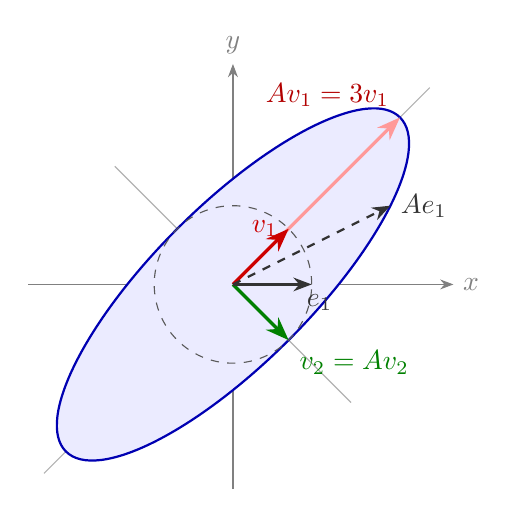
\begin{tikzpicture}[x=1cm, y=1cm, >=Stealth]
        \draw[->, gray] (-2.6,0) -- (2.8,0) node[right] {$x$};
        \draw[->, gray] (0,-2.6) -- (0,2.8) node[above] {$y$};
        \draw[gray!60, thin] (-2.4,-2.4) -- (2.5,2.5);
        \draw[gray!60, thin] (-1.5,1.5) -- (1.5,-1.5);
        \fill[blue!8, rotate=45] (0,0) ellipse [x radius=3, y radius=1];
        \draw[blue!70!black, thick, rotate=45] (0,0) ellipse [x radius=3, y radius=1];
        \draw[gray!70!black, dashed] (0,0) circle (1);
        \draw[->, very thick, red!40] (0,0) -- (2.121,2.121) node[above left, red!70!black] {$Av_1 = 3v_1$};
        \draw[->, very thick, red!80!black] (0,0) -- (0.707,0.707) node[left] {$v_1$};
        \draw[->, very thick, green!50!black] (0,0) -- (0.707,-0.707) node[below right] {$v_2 = Av_2$};
        \draw[->, thick, gray!40!black] (0,0) -- (1,0);
        \node[gray!40!black, below] at (1.1,0) {$e_1$};
        \draw[->, thick, gray!40!black, dashed] (0,0) -- (2,1) node[right] {$Ae_1$};
    \end{tikzpicture}
    \caption[Eigenvectors]{The matrix $A = \begin{pmatrix} 2 & 1 \\ 1 & 2 \end{pmatrix}$ maps the unit circle (dashed) to an ellipse (blue). The eigenvector $v_1 = \frac{1}{\sqrt{2}}(1, 1)$ is stretched by its eigenvalue $3$, and the eigenvector $v_2 = \frac{1}{\sqrt{2}}(1, -1)$ is left unchanged, since its eigenvalue is $1$. The vector $e_1$ is not an eigenvector: its image $Ae_1 = (2, 1)$ points in a different direction.}
    \label{L1-fig:eigen}
\end{figure}

\begin{definition}[Eigenspace]
    For $\lambda \in \mathbb{R}$, the set
    \[E_\lambda = \{v \in \mathbb{R}^n : Av = \lambda v\} = \Null(A - \lambda I_n)\]
    is called the eigenspace of $A$ for $\lambda$. It is a subspace of $\mathbb{R}^n$ (Theorem~\ref{L1-thm:kerim}), and $\lambda$ is an eigenvalue if and only if $E_\lambda \neq \{0\}$; in that case, $E_\lambda$ consists of the eigenvectors for $\lambda$ together with $0$.
\end{definition}

\begin{proposition}\label{L1-prop:eigen-det}
    A number $\lambda$ is an eigenvalue of $A$ if and only if $A - \lambda I_n$ is not invertible, if and only if $\det(A - \lambda I_n) = 0$. In particular, $0$ is an eigenvalue of $A$ if and only if $A$ is not invertible.
\end{proposition}

\begin{proof}
    $Av = \lambda v$ means $(A - \lambda I_n)v = 0$. So $\lambda$ is an eigenvalue if and only if $\Null(A - \lambda I_n) \neq \{0\}$, which by Corollary~\ref{L1-cor:invertible-rank} means that $A - \lambda I_n$ is not invertible, or equivalently, that $\det(A - \lambda I_n) = 0$.
\end{proof}

\subsection{The characteristic polynomial}

\begin{definition}[Characteristic polynomial]
    The characteristic polynomial of $A$ is
    \[p_A(\lambda) = \det(A - \lambda I_n).\]
\end{definition}

Expanding the determinant shows that $p_A(\lambda)$ is a polynomial of degree $n$ in $\lambda$, with leading term $(-\lambda)^n$, which comes from the product $(A_{11} - \lambda) \cdots (A_{nn} - \lambda)$ of the diagonal entries. By Proposition~\ref{L1-prop:eigen-det}, the eigenvalues of $A$ are exactly the real roots of $p_A$. So, to find the eigenvalues and eigenvectors of $A$:
\begin{enumerate}
    \item compute $p_A(\lambda)$ and find its real roots $\lambda$;
    \item for each root $\lambda$, find the eigenspace $E_\lambda = \Null(A - \lambda I_n)$ by row reduction.
\end{enumerate}

\begin{proposition}\label{L1-prop:char-poly-2x2}
    For a $2 \times 2$ matrix $A$, $p_A(\lambda) = \lambda^2 - \tr(A)\, \lambda + \det(A)$.
\end{proposition}

\begin{proof}
    For $A = \begin{pmatrix} a & b \\ c & d \end{pmatrix}$, we get $p_A(\lambda) = (a - \lambda)(d - \lambda) - bc = \lambda^2 - (a + d)\lambda + (ad - bc)$.
\end{proof}

\begin{example}\label{L1-ex:eigen-2x2}
    For $A = \begin{pmatrix} 2 & 1 \\ 1 & 2 \end{pmatrix}$, we get $p_A(\lambda) = \lambda^2 - 4\lambda + 3 = (\lambda - 1)(\lambda - 3)$, so the eigenvalues are $1$ and $3$. The eigenspaces are
    \[E_3 = \Null \begin{pmatrix} -1 & 1 \\ 1 & -1 \end{pmatrix} = \Span\{(1, 1)^\top\}, \qquad E_1 = \Null \begin{pmatrix} 1 & 1 \\ 1 & 1 \end{pmatrix} = \Span\{(1, -1)^\top\},\]
    in agreement with Example~\ref{L1-ex:eigen-first}.
\end{example}

\begin{example}\label{L1-ex:eigen-3x3}
    Let $J = \begin{pmatrix} 0 & 1 & 1 \\ 1 & 0 & 1 \\ 1 & 1 & 0 \end{pmatrix}$. Expanding along the first row,
    \[p_J(\lambda) = \det \begin{pmatrix} -\lambda & 1 & 1 \\ 1 & -\lambda & 1 \\ 1 & 1 & -\lambda \end{pmatrix} = -\lambda(\lambda^2 - 1) - (-\lambda - 1) + (1 + \lambda) = -\lambda^3 + 3\lambda + 2 = -(\lambda - 2)(\lambda + 1)^2.\]
    So the eigenvalues are $2$ and $-1$. Row reduction gives
    \[E_2 = \Null(J - 2I_3) = \Span\{(1, 1, 1)^\top\}, \qquad E_{-1} = \Null(J + I_3) = \Null \begin{pmatrix} 1 & 1 & 1 \\ 1 & 1 & 1 \\ 1 & 1 & 1 \end{pmatrix}.\]
    The eigenspace $E_{-1}$ is the plane $x + y + z = 0$, with basis $(1, -1, 0)^\top$, $(1, 0, -1)^\top$.
\end{example}

\begin{proposition}\label{L1-prop:eigen-triangular}
    The eigenvalues of a triangular matrix are its diagonal entries.
\end{proposition}

\begin{proof}
    If $A$ is triangular, so is $A - \lambda I_n$, and by Corollary~\ref{L1-cor:det-easy}, $p_A(\lambda) = (A_{11} - \lambda) \cdots (A_{nn} - \lambda)$.
\end{proof}

\begin{example}[Eigenvectors from geometry]\label{L1-ex:eigen-geometric}
    Geometric intuition often tells us the eigenvectors without any computation. The shear and the rotations below also appear in the gallery of Figure~\ref{L1-fig:gallery}.
    \begin{itemize}
        \item The projection onto the $x$-axis, $\begin{pmatrix} 1 & 0 \\ 0 & 0 \end{pmatrix}$, has the eigenvalue $1$ with eigenspace the $x$-axis, and the eigenvalue $0$ with eigenspace the $y$-axis.
        \item The reflection in the line $y = x$, $\begin{pmatrix} 0 & 1 \\ 1 & 0 \end{pmatrix}$, fixes this line (eigenvalue $1$) and flips the line $y = -x$ (eigenvalue $-1$).
        \item The shear $\begin{pmatrix} 1 & 1 \\ 0 & 1 \end{pmatrix}$ has $p(\lambda) = (1 - \lambda)^2$, so its only eigenvalue is $1$, and $E_1 = \Null \begin{pmatrix} 0 & 1 \\ 0 & 0 \end{pmatrix} = \Span\{e_1\}$: only the horizontal direction is preserved.
        \item The rotation $R_\theta$ has $p(\lambda) = \lambda^2 - 2\cos\theta\, \lambda + 1$, with discriminant $4\cos^2\theta - 4 < 0$ unless $\theta$ is a multiple of $\pi$. So a rotation by an angle other than $0$ or $\pi$ has no real eigenvalues: it does not preserve any direction.
    \end{itemize}
\end{example}

\begin{remark}[Complex eigenvalues]
    By the fundamental theorem of algebra (which we state without proof), every polynomial of degree $n$ factors into $n$ linear factors over $\mathbb{C}$. Hence
    \[p_A(\lambda) = (\lambda_1 - \lambda)(\lambda_2 - \lambda) \cdots (\lambda_n - \lambda)\]
    for some $\lambda_1, \ldots, \lambda_n \in \mathbb{C}$, which are called the complex eigenvalues of $A$, counted with multiplicity. For example, the rotation $R_\theta$ has the complex eigenvalues $\cos\theta \pm i\sin\theta$, with complex eigenvectors $(1, \mp i)^\top$. In these notes, ``eigenvalue'' means a real eigenvalue unless we say otherwise.
\end{remark}

\begin{theorem}\label{L1-thm:trace-det-eigen}
    Let $\lambda_1, \ldots, \lambda_n \in \mathbb{C}$ be the complex eigenvalues of $A$, counted with multiplicity. Then
    \[\det(A) = \lambda_1 \lambda_2 \cdots \lambda_n \qquad \text{and} \qquad \tr(A) = \lambda_1 + \lambda_2 + \cdots + \lambda_n.\]
\end{theorem}

\begin{proof}
    Setting $\lambda = 0$ in the factorization of $p_A$ gives $\det(A) = p_A(0) = \lambda_1 \cdots \lambda_n$. For the trace, we compare the coefficients of $\lambda^{n-1}$. In $(\lambda_1 - \lambda) \cdots (\lambda_n - \lambda)$, this coefficient is $(-1)^{n-1}(\lambda_1 + \cdots + \lambda_n)$. In $\det(A - \lambda I_n)$, one can check by induction on $n$, using the cofactor expansion, that only the product $(A_{11} - \lambda) \cdots (A_{nn} - \lambda)$ of the diagonal entries contributes to $\lambda^{n-1}$, since every other term contains at most $n - 2$ diagonal entries. So the coefficient is $(-1)^{n-1}(A_{11} + \cdots + A_{nn}) = (-1)^{n-1}\tr(A)$.
\end{proof}

\begin{example}
    For the matrix of Example~\ref{L1-ex:eigen-2x2}, $1 + 3 = 4 = \tr(A)$ and $1 \cdot 3 = 3 = \det(A)$. For the matrix $J$ of Example~\ref{L1-ex:eigen-3x3}, $2 + (-1) + (-1) = 0 = \tr(J)$ and $2 \cdot (-1) \cdot (-1) = 2 = \det(J)$. For the rotation $R_\theta$, $(\cos\theta + i\sin\theta)(\cos\theta - i\sin\theta) = 1 = \det(R_\theta)$ and the sum is $2\cos\theta = \tr(R_\theta)$.
\end{example}

\begin{proposition}\label{L1-prop:eigen-related}
    Let $Av = \lambda v$ with $v \neq 0$. Then:
    \begin{enumerate}
        \item $A^k v = \lambda^k v$ for every $k \geq 1$;
        \item if $A$ is invertible, then $\lambda \neq 0$ and $A^{-1} v = \frac{1}{\lambda} v$;
        \item $(A + cI_n)v = (\lambda + c)v$ for every $c \in \mathbb{R}$.
    \end{enumerate}
    Moreover, $A$ and $A^\top$ have the same characteristic polynomial, and hence the same eigenvalues.
\end{proposition}

\begin{proof}
    (1) By induction, $A^k v = A(A^{k-1} v) = A(\lambda^{k-1} v) = \lambda^{k-1} Av = \lambda^k v$. (2) $\lambda \neq 0$ by Proposition~\ref{L1-prop:eigen-det}, and applying $A^{-1}$ to $Av = \lambda v$ gives $v = \lambda A^{-1}v$. (3) $(A + cI_n)v = Av + cv = (\lambda + c)v$. Finally, $\det(A^\top - \lambda I_n) = \det\big((A - \lambda I_n)^\top\big) = \det(A - \lambda I_n)$.
\end{proof}

Note that $A$ and $A^\top$ usually have different eigenvectors; for the shear, $E_1 = \Span\{e_1\}$ for $A$, but $E_1 = \Span\{e_2\}$ for $A^\top$.

\subsection{Diagonalization}

\begin{theorem}\label{L1-thm:eigen-independent}
    Eigenvectors $v_1, \ldots, v_k$ of $A$ for distinct eigenvalues $\lambda_1, \ldots, \lambda_k$ are linearly independent.
\end{theorem}

\begin{proof}
    Suppose not, and let $m$ be the smallest index such that $v_1, \ldots, v_m$ are linearly dependent. Then $m \geq 2$ (since $v_1 \neq 0$), $v_1, \ldots, v_{m-1}$ are linearly independent, and $v_m = c_1 v_1 + \cdots + c_{m-1} v_{m-1}$ for some scalars $c_i$. Applying $A - \lambda_m I_n$ to both sides gives
    \[0 = c_1 (\lambda_1 - \lambda_m) v_1 + \cdots + c_{m-1} (\lambda_{m-1} - \lambda_m) v_{m-1}.\]
    By independence, $c_i (\lambda_i - \lambda_m) = 0$, and since the eigenvalues are distinct, $c_i = 0$ for all $i$. But then $v_m = 0$, a contradiction.
\end{proof}

\begin{definition}[Diagonalizable matrix]
    A matrix $A$ is called diagonalizable if there are an invertible matrix $P$ and a diagonal matrix $D$ with
    \[A = PDP^{-1}, \qquad \text{or equivalently} \qquad P^{-1}AP = D.\]
    More generally, two matrices $A$ and $B$ are called similar if $B = P^{-1}AP$ for some invertible matrix $P$.
\end{definition}

Similar matrices have the same characteristic polynomial, since by the product rule for determinants,
\[\det(P^{-1}AP - \lambda I_n) = \det\big(P^{-1}(A - \lambda I_n)P\big) = \det(P^{-1})\det(A - \lambda I_n)\det(P) = \det(A - \lambda I_n).\]
Hence they also have the same eigenvalues, trace and determinant (compare Subsection~\ref{L1-subsec:trace-det}).

\begin{theorem}[Diagonalization]\label{L1-thm:diagonalization}
    An $n \times n$ matrix $A$ is diagonalizable if and only if it has $n$ linearly independent eigenvectors $p_1, \ldots, p_n$. In this case, $A = PDP^{-1}$, where $P$ is the matrix with columns $p_1, \ldots, p_n$, and $D = \diag(\lambda_1, \ldots, \lambda_n)$ contains the corresponding eigenvalues, in the same order.
\end{theorem}

\begin{proof}
    Let $P$ have columns $p_1, \ldots, p_n$, and let $D = \diag(\lambda_1, \ldots, \lambda_n)$. By the column-by-column description of matrix multiplication, the $i$-th column of $AP$ is $Ap_i$, and the $i$-th column of $PD$ is $\lambda_i p_i$. So $AP = PD$ if and only if $Ap_i = \lambda_i p_i$ for all $i$. Moreover, $P$ is invertible if and only if $\Null(P) = \{0\}$ (Corollary~\ref{L1-cor:invertible-rank}), i.e., if and only if its columns are linearly independent. Hence: if $p_1, \ldots, p_n$ are linearly independent eigenvectors, then $AP = PD$ with $P$ invertible, so $A = PDP^{-1}$. Conversely, if $A = PDP^{-1}$, then $AP = PD$, so the columns of $P$ are eigenvectors (they are nonzero, since $P$ is invertible), and they are linearly independent.
\end{proof}

\begin{corollary}\label{L1-cor:distinct-eigenvalues}
    If an $n \times n$ matrix has $n$ distinct real eigenvalues, then it is diagonalizable.
\end{corollary}

\begin{proof}
    Choose an eigenvector for each eigenvalue. By Theorem~\ref{L1-thm:eigen-independent}, these $n$ eigenvectors are linearly independent.
\end{proof}

\begin{remark}
    If $A = PDP^{-1}$, then the columns $p_1, \ldots, p_n$ of $P$ form a basis $\mathcal{B}$ of $\mathbb{R}^n$, and $P^{-1}v = [v]_{\mathcal{B}}$ is the coordinate vector of $v$ with respect to this basis. So $P^{-1}AP = D$ says that the matrix of $T_A$ with respect to the basis of eigenvectors is diagonal (Subsection~\ref{L1-subsec:inverse}): in these coordinates, $T_A$ simply multiplies the $i$-th coordinate by $\lambda_i$.
\end{remark}

\begin{example}
    For the matrix $A$ of Example~\ref{L1-ex:eigen-2x2},
    \[A = \begin{pmatrix} 2 & 1 \\ 1 & 2 \end{pmatrix} = \underbrace{\begin{pmatrix} 1 & 1 \\ 1 & -1 \end{pmatrix}}_{P} \underbrace{\begin{pmatrix} 3 & 0 \\ 0 & 1 \end{pmatrix}}_{D} \underbrace{\frac{1}{2}\begin{pmatrix} 1 & 1 \\ 1 & -1 \end{pmatrix}}_{P^{-1}}.\]
\end{example}

Not every matrix is diagonalizable. To see what can go wrong, we count eigenvectors.

\begin{definition}[Multiplicities]
    Let $\lambda$ be an eigenvalue of $A$. Its algebraic multiplicity is its multiplicity as a root of $p_A$, i.e., the number of times the factor $(\lambda - \cdot)$ appears in $p_A$. Its geometric multiplicity is $\dim E_\lambda = n - \rank(A - \lambda I_n)$ (by the rank--nullity theorem).
\end{definition}

\begin{theorem}\label{L1-thm:multiplicities}
    For every eigenvalue, $1 \leq \text{geometric multiplicity} \leq \text{algebraic multiplicity}$. Moreover, $A$ is diagonalizable if and only if $p_A$ has $n$ real roots (counted with multiplicity), and the geometric multiplicity of every eigenvalue equals its algebraic multiplicity.
\end{theorem}

We state this theorem without proof. The second part says that we need ``enough'' eigenvectors: by Theorem~\ref{L1-thm:eigen-independent}, bases of the different eigenspaces together form a linearly independent set, and $A$ is diagonalizable exactly when this set has $n$ elements.

\begin{example}
    \begin{itemize}
        \item The matrix $J$ of Example~\ref{L1-ex:eigen-3x3} has the eigenvalue $-1$ with algebraic multiplicity $2$, and geometric multiplicity $3 - \rank(J + I_3) = 3 - 1 = 2$. So $J$ is diagonalizable:
        \[J = PDP^{-1} \qquad \text{with} \qquad P = \begin{pmatrix} 1 & 1 & 1 \\ 1 & -1 & 0 \\ 1 & 0 & -1 \end{pmatrix}, \quad D = \diag(2, -1, -1).\]
        \item The shear $\begin{pmatrix} 1 & 1 \\ 0 & 1 \end{pmatrix}$ has the eigenvalue $1$ with algebraic multiplicity $2$, but geometric multiplicity $1$. So it is not diagonalizable.
        \item A rotation $R_\theta$ with $\theta$ not a multiple of $\pi$ has no real eigenvalues, so it is not diagonalizable with real matrices $P$ and $D$. (It is diagonalizable with complex matrices.)
    \end{itemize}
\end{example}

\begin{remark}
    Symmetric matrices are always diagonalizable, and their eigenvectors can even be chosen to be orthonormal. This is the spectral theorem, which we prove in Lecture~2 once we have inner products.
\end{remark}

\subsection{Powers of matrices and applications}

\begin{proposition}\label{L1-prop:powers}
    If $A = PDP^{-1}$ with $D = \diag(\lambda_1, \ldots, \lambda_n)$, then for every $k \geq 1$,
    \[A^k = P D^k P^{-1}, \qquad \text{where} \quad D^k = \diag(\lambda_1^k, \ldots, \lambda_n^k).\]
\end{proposition}

\begin{proof}
    $A^k = (PDP^{-1})(PDP^{-1}) \cdots (PDP^{-1}) = PD(P^{-1}P)D(P^{-1}P) \cdots DP^{-1} = PD^kP^{-1}$, and $D^k$ is computed entry by entry, since products of diagonal matrices are computed on the diagonal (Subsection~\ref{L1-subsec:special}).
\end{proof}

\begin{example}
    For $A = \begin{pmatrix} 2 & 1 \\ 1 & 2 \end{pmatrix}$,
    \[A^k = \begin{pmatrix} 1 & 1 \\ 1 & -1 \end{pmatrix} \begin{pmatrix} 3^k & 0 \\ 0 & 1 \end{pmatrix} \frac{1}{2}\begin{pmatrix} 1 & 1 \\ 1 & -1 \end{pmatrix} = \frac{1}{2} \begin{pmatrix} 3^k + 1 & 3^k - 1 \\ 3^k - 1 & 3^k + 1 \end{pmatrix}.\]
    Computing $A^{100}$ by multiplying $A$ with itself $99$ times would be much more work.
\end{example}

\begin{example}[Fibonacci numbers]\label{L1-ex:binet}
    The Fibonacci numbers $F_0 = 0$, $F_1 = 1$, $F_{n+1} = F_n + F_{n-1}$ satisfy
    \[\begin{pmatrix} F_{n+1} \\ F_n \end{pmatrix} = M \begin{pmatrix} F_n \\ F_{n-1} \end{pmatrix} = \cdots = M^n \begin{pmatrix} 1 \\ 0 \end{pmatrix}, \qquad \text{where} \quad M = \begin{pmatrix} 1 & 1 \\ 1 & 0 \end{pmatrix}.\]
    The characteristic polynomial of $M$ is $\lambda^2 - \lambda - 1$, with the roots
    \[\varphi = \frac{1 + \sqrt{5}}{2} \approx 1.618 \quad \text{(the golden ratio)} \qquad \text{and} \qquad \psi = \frac{1 - \sqrt{5}}{2} \approx -0.618.\]
    One checks that $(\varphi, 1)^\top$ and $(\psi, 1)^\top$ are eigenvectors, and that $(1, 0)^\top = \frac{1}{\sqrt{5}}\big((\varphi, 1)^\top - (\psi, 1)^\top\big)$, since $\varphi - \psi = \sqrt{5}$. By Proposition~\ref{L1-prop:eigen-related},
    \[\begin{pmatrix} F_{n+1} \\ F_n \end{pmatrix} = \frac{1}{\sqrt{5}}\left(\varphi^n \begin{pmatrix} \varphi \\ 1 \end{pmatrix} - \psi^n \begin{pmatrix} \psi \\ 1 \end{pmatrix}\right), \qquad \text{so} \qquad F_n = \frac{\varphi^n - \psi^n}{\sqrt{5}}.\]
    This is Binet's formula. Since $|\psi| < 1$, the term $\psi^n$ quickly becomes tiny, and $F_n$ is the integer closest to $\varphi^n / \sqrt{5}$. In particular, $F_{n+1}/F_n \to \varphi$.
\end{example}

\begin{example}[Markov chains]\label{L1-ex:markov}
    Suppose that the weather is either sunny or rainy, and that a sunny day is followed by a sunny day with probability $0.9$, while a rainy day is followed by a sunny day with probability $0.5$. If $x_k = (s_k, r_k)^\top$ contains the probabilities that day $k$ is sunny or rainy, then
    \[x_{k+1} = A x_k, \qquad \text{where} \quad A = \begin{pmatrix} 0.9 & 0.5 \\ 0.1 & 0.5 \end{pmatrix}.\]
    The columns of $A$ are probability vectors (nonnegative entries summing to $1$). By Proposition~\ref{L1-prop:char-poly-2x2}, $p_A(\lambda) = \lambda^2 - 1.4\lambda + 0.4 = (\lambda - 1)(\lambda - 0.4)$, with eigenvectors $(5, 1)^\top$ for $\lambda = 1$ and $(1, -1)^\top$ for $\lambda = 0.4$. If today is rainy, then $x_0 = (0, 1)^\top = \big(\frac{5}{6}, \frac{1}{6}\big)^\top - \frac{5}{6}(1, -1)^\top$, so
    \[x_k = A^k x_0 = \begin{pmatrix} 5/6 \\ 1/6 \end{pmatrix} - \frac{5}{6}\, (0.4)^k \begin{pmatrix} 1 \\ -1 \end{pmatrix} \longrightarrow \begin{pmatrix} 5/6 \\ 1/6 \end{pmatrix} \qquad (k \to \infty).\]
    In the long run, $\frac{5}{6}$ of the days are sunny, whatever the weather today. The limit $\big(\frac{5}{6}, \frac{1}{6}\big)^\top$ is the eigenvector for the eigenvalue $1$, scaled to be a probability vector; it is called the stationary distribution of the Markov chain.
\end{example}

\begin{remark}[PageRank and power iteration]
    The PageRank algorithm, originally used by Google to rank web pages, models a random surfer who follows a random link on each page. The importance of a page is its probability in the stationary distribution of this Markov chain, i.e., an entry of the eigenvector for the eigenvalue $1$ of a huge matrix. Such eigenvectors are computed by power iteration: if $A$ has an eigenvalue $\lambda_1$ with $|\lambda_1| > |\lambda_i|$ for all other eigenvalues, and $A$ is diagonalizable with eigenvectors $v_1, \ldots, v_n$, then writing $x = c_1 v_1 + \cdots + c_n v_n$ gives
    \[A^k x = \lambda_1^k \Big(c_1 v_1 + \sum_{i \geq 2} c_i \Big(\frac{\lambda_i}{\lambda_1}\Big)^k v_i\Big),\]
    so after rescaling, $A^k x$ points more and more in the direction of $v_1$ (if $c_1 \neq 0$). You will implement this in Programming Exercise~P10.
\end{remark}

\section{Key Takeaways}
\begin{itemize}[leftmargin=*]
	\item A field is a set of ``numbers'' in which we can add, subtract, multiply, and divide by nonzero elements. $\mathbb{Q}$, $\mathbb{R}$ and $\mathbb{C}$ are fields; $\mathbb{Z}$ is not.
	\item A vector space over a field $\mathbb{F}$ is a set of vectors that can be added and multiplied by scalars from $\mathbb{F}$, subject to the vector space axioms. Examples: $\mathbb{F}$ itself, products $V \times W$, $\mathbb{R}^n$, and the polynomials $\mathbb{R}[x]$.
	\item A basis is a linearly independent set that spans the space; every vector is a unique linear combination of the basis vectors. All bases of a finite-dimensional space have the same number of vectors, the dimension: $\dim \mathbb{R}^n = n$, while $\mathbb{R}[x]$ is infinite-dimensional.
	\item A linear transformation $T: V \to W$ preserves addition and scalar multiplication, and $T(0_V) = 0_W$. Its kernel is a subspace of $V$, and its image is a subspace of $W$.
	\item An isomorphism is a bijective linear transformation, i.e., one with $\ker(T) = \{0\}$ and $\im(T) = W$. Via coordinates, every $n$-dimensional real vector space is isomorphic to $\mathbb{R}^n$, and $V \cong W$ if and only if $\dim V = \dim W$, if and only if some linear transformation $V \to W$ is represented by an invertible matrix.
	\item Every linear transformation $T: \mathbb{R}^n \to \mathbb{R}^m$ is multiplication by an $m \times n$ matrix $A$, whose $i$-th column is $T(e_i)$.
	\item Matrices of the same size are added entry by entry. The product of an $m \times n$ and an $n \times p$ matrix is the $m \times p$ matrix with $(AB)_{ij} = \sum_k A_{ik} B_{kj}$; it represents the composition $T_A \circ T_B$. Matrix multiplication is associative but not commutative, and $(AB)^\top = B^\top A^\top$.
	\item A square matrix $A$ is invertible if $AB = BA = I_n$ for some matrix $B = A^{-1}$; then $Ax = b$ has the unique solution $x = A^{-1}b$, and $(AB)^{-1} = B^{-1}A^{-1}$. The inverse is computed without determinants by row reducing $(A \mid I_n)$ to $(I_n \mid A^{-1})$.
	\item Diagonal, upper and lower triangular, symmetric ($A^\top = A$) and skew-symmetric ($A^\top = -A$) matrices form subspaces of $\mathbb{R}^{n \times n}$. The invertible matrices $\mathrm{GL}(n, \mathbb{R})$ and the orthogonal matrices $\mathrm{O}(n)$ (with $Q^\top Q = I_n$, so $Q^{-1} = Q^\top$) do not form subspaces, but they contain $I_n$ and are closed under multiplication and inverses: they are matrix groups.
	\item The trace $\tr(A) = \sum_i A_{ii}$ is linear and satisfies $\tr(AB) = \tr(BA)$. The determinant is defined by cofactor expansion and is best computed by row reduction to triangular form; it satisfies $\det(AB) = \det(A)\det(B)$ and $\det(A^\top) = \det(A)$, and $|\det(A)|$ is the factor by which $T_A$ scales areas and volumes.
	\item Elementary row operations bring a matrix into (reduced) row echelon form. They do not change the null space or the row space, but they can change the column space; the pivot columns of the original matrix form a basis of its column space.
	\item $\rank(A) = \dim \col(A) = \dim \row(A)$ is the number of pivots, and $\rank(A) + \dim \Null(A) = n$ for every $m \times n$ matrix $A$.
	\item For an $n \times n$ matrix $A$: $A$ is invertible $\iff$ $\Null(A) = \{0\}$ $\iff$ $\rank(A) = n$ $\iff$ $\RREF(A) = I_n$ $\iff$ $\det(A) \neq 0$.
	\item The dual space $V^*$ consists of the linear functionals $V \to \mathbb{F}$; on $\mathbb{R}^n$, these are the row vectors. A basis $b_1, \ldots, b_n$ has a dual basis $b^1, \ldots, b^n$ with $b^i(b_j) = \delta_{ij}$ (in $\mathbb{R}^n$: the rows of $P^{-1}$), and $\dim V^* = \dim V$. The dual map $T^*(\psi) = \psi \circ T$ is represented by the transpose $A^\top$. A system $Ax = b$ is solvable if and only if $yb = 0$ for all rows $y$ with $yA = 0$.
	\item The quotient space $V/U$ consists of the cosets $v + U$, where $v + U = w + U$ if and only if $v - w \in U$; it has dimension $\dim V - \dim U$. First isomorphism theorem: $V/\ker(T) \cong \im(T)$, which gives rank--nullity for every linear map. Second: $(U + W)/W \cong U/(U \cap W)$, so $\dim(U + W) + \dim(U \cap W) = \dim U + \dim W$. Third: $(V/U)/(W/U) \cong V/W$.
	\item An eigenvector $v \neq 0$ of $A$ satisfies $Av = \lambda v$; the eigenvalues are the roots of the characteristic polynomial $\det(A - \lambda I_n)$, and the eigenspace $E_\lambda = \Null(A - \lambda I_n)$ is found by row reduction. The (complex) eigenvalues add up to $\tr(A)$ and multiply to $\det(A)$.
	\item $A$ is diagonalizable, $A = PDP^{-1}$, exactly when it has $n$ linearly independent eigenvectors (the columns of $P$); this holds, for example, when $A$ has $n$ distinct eigenvalues. Then $A^k = PD^kP^{-1}$, which explains Fibonacci numbers, the long-run behavior of Markov chains, and power iteration (PageRank).
\end{itemize}

\section{Exercises}\label{L1-sec:exercises}
\begin{enumerate}[leftmargin=*]
	\item\label{L1-ex:axioms} Using only the vector space axioms, prove that in every vector space $V$ over a field $\mathbb{F}$:
	\begin{enumerate}
		\item $0 \cdot v = 0_V$ for every $v \in V$. (Hint: $0 \cdot v = (0 + 0) \cdot v$.)
		\item $(-1) \cdot v = -v$ for every $v \in V$. (Hint: compute $v + (-1) \cdot v$.)
	\end{enumerate}
	\item Which of the following subsets of $\mathbb{R}^2$ are subspaces? Justify your answers.
	\begin{enumerate}
		\item $\{(x, y) \in \mathbb{R}^2 : y = 2x\}$;
		\item $\{(x, y) \in \mathbb{R}^2 : y = 2x + 1\}$;
		\item $\{(x, y) \in \mathbb{R}^2 : xy = 0\}$.
	\end{enumerate}
	\item Show that $\{(1, 2), (3, 4)\}$ is a basis of $\mathbb{R}^2$, and write $(5, 6)$ as a linear combination of these two vectors.
	\item Let $\mathbb{R}[x]_{\leq 2}$ be the set of polynomials with real coefficients of degree at most $2$. Show that it is a subspace of $\mathbb{R}[x]$, and find its dimension.
	\item Let $T: \mathbb{R}^3 \to \mathbb{R}^3$ be defined by $T(x, y, z) = (x + y, y + z, x + 2y + z)$. Find the matrix $A$ of $T$ and $\RREF(A)$. Then find a basis of $\Null(A)$, a basis of $\col(A)$, and $\rank(A)$, and check that your answers agree with the rank--nullity theorem.
	\item Write down explicit isomorphisms $\mathbb{R}^{2 \times 2} \to \mathbb{R}^4$ and $\mathrm{Sym}_2 \to \mathbb{R}^3$, and prove that they are isomorphisms. Are $\mathbb{R}^{2 \times 2}$ and $\mathrm{Sym}_2$ isomorphic?
	\item Let $A = \begin{pmatrix} 1 & 2 \\ 3 & 4 \end{pmatrix}$ and $B = \begin{pmatrix} 0 & 1 \\ 1 & 0 \end{pmatrix}$. Compute $AB$ and $BA$. Describe in words what multiplying a $2 \times 2$ matrix by $B$ from the left does, and what multiplying it by $B$ from the right does.
	\item Use the Gauss--Jordan method to find the inverse of
	\[A = \begin{pmatrix}
		1 & 2 & 3 \\
		0 & 1 & 4 \\
		5 & 6 & 0
	\end{pmatrix},\]
	and check your answer.
	\item Show that the matrix $F$ from Example~\ref{L1-ex:F} is not invertible, and find a nonzero vector $x$ with $Fx = 0$.
	\item Let $A$ be an $n \times n$ matrix with $A^2 = A$ (where $A^2 = AA$) and $A \neq I_n$. Show that $A$ is not invertible.
	\item Show that an upper triangular matrix is invertible if and only if all of its diagonal entries are nonzero, in two ways: using Theorem~\ref{L1-thm:invertible}, and using determinants.
	\item Compute the determinant of
	\[A = \begin{pmatrix}
		2 & 0 & 1 \\
		1 & 3 & 2 \\
		1 & 1 & 1
	\end{pmatrix}\]
	in two ways: by cofactor expansion, and by row reduction. Is $A$ invertible?
	\item Let $A$ be a skew-symmetric $n \times n$ matrix, where $n$ is odd. Show that $\det(A) = 0$. (Hint: compute $\det(A^\top)$ in two ways.)
	\item Show that $\tr(ABC) = \tr(CAB)$ for all $n \times n$ matrices $A$, $B$, $C$, but find $2 \times 2$ matrices with $\tr(ABC) \neq \tr(ACB)$.
	\item Find the eigenvalues and eigenspaces of $A = \begin{pmatrix} 4 & 1 \\ 2 & 3 \end{pmatrix}$. Diagonalize $A$, and use the diagonalization to find a formula for $A^k$.
	\item Show that $A = \begin{pmatrix} 3 & 1 \\ 0 & 3 \end{pmatrix}$ is not diagonalizable. Find all of its eigenvectors.
	\item Find the complex eigenvalues of the rotation by $90^\circ$, $\begin{pmatrix} 0 & -1 \\ 1 & 0 \end{pmatrix}$, and check Theorem~\ref{L1-thm:trace-det-eigen} for this matrix.
	\item Let $A$ be a $3 \times 3$ matrix with eigenvalues $1$, $2$ and $3$. Compute $\tr(A^2)$, $\det(A)$ and $\det(A^{-1})$. (Hint: $A$ is diagonalizable.)
	\item Let $A$ be an $n \times n$ matrix and $\lambda$ an eigenvalue of $A$.
	\begin{enumerate}
		\item Show that if $A^2 = A$, then $\lambda = 0$ or $\lambda = 1$.
		\item Show that if $A^k = 0$ for some $k \geq 1$, then $\lambda = 0$.
		\item Show that if $A$ is orthogonal, then $\lambda = 1$ or $\lambda = -1$.
	\end{enumerate}
	\item A Markov chain has the transition matrix $A = \begin{pmatrix} 0.8 & 0.3 \\ 0.2 & 0.7 \end{pmatrix}$. Find its eigenvalues and its stationary distribution, and describe what happens to $A^k x_0$ as $k \to \infty$ for a probability vector $x_0$.
	\item Find the dual basis of the basis $(1, 0, 0)^\top$, $(1, 1, 0)^\top$, $(1, 1, 1)^\top$ of $\mathbb{R}^3$, and check that $b^i(b_j) = \delta_{ij}$.
	\item On $V = \mathbb{R}[x]_{\leq 2}$, consider the functionals $\varphi_1(p) = p(0)$, $\varphi_2(p) = p'(0)$ and $\varphi_3(p) = \int_{-1}^1 p(x)\, dx$. Show that $\varphi_1, \varphi_2, \varphi_3$ is a basis of $V^*$, and find the basis $q_1, q_2, q_3$ of $V$ whose dual basis it is, i.e., with $\varphi_i(q_j) = \delta_{ij}$.
	\item Let $T: \mathbb{R}^2 \to \mathbb{R}^2$, $T(x, y) = (x + 2y, 3y)$. Compute $T^*(\psi)$ for the coordinate functionals $\psi(x, y) = x$ and $\psi(x, y) = y$, and check that the matrix of $T^*$ with respect to the dual of the standard basis is the transpose of the matrix of $T$.
	\item Let $\varphi$ and $\psi$ be nonzero linear functionals on a finite-dimensional vector space with $\ker(\varphi) = \ker(\psi)$. Show that $\psi = c\varphi$ for some $c \neq 0$. (Hint: choose $v$ with $\varphi(v) = 1$, and show that every vector is of the form $w + tv$ with $w \in \ker(\varphi)$.)
	\item Let $U = \Span\{(1, 0, 1)^\top, (0, 1, 1)^\top\} \subseteq \mathbb{R}^3$. Show that the cosets of $U$ are the planes $x_1 + x_2 - x_3 = c$, and that $x + U \mapsto x_1 + x_2 - x_3$ is an isomorphism $\mathbb{R}^3/U \to \mathbb{R}$. Check Theorem~\ref{L1-thm:quotient-dim}.
	\item Use the first isomorphism theorem and the map $A \mapsto \frac{1}{2}(A + A^\top)$ to show that $\mathbb{R}^{n \times n}/\mathrm{Skew}_n \cong \mathrm{Sym}_n$, and check that the dimensions agree.
	\item Let $U$ and $W$ be $3$-dimensional subspaces of $\mathbb{R}^5$. Show that $U \cap W \neq \{0\}$. Which values can $\dim(U \cap W)$ take?
	\item Show that $V/U = \{0\}$ if and only if $U = V$, and that $V/\{0\} \cong V$.
\end{enumerate}

\section{Programming Exercises}\label{L1-sec:programming}

% Inline code cannot be hyphenated, so allow a little extra stretch in this section.
\setlength{\emergencystretch}{3em}

In these exercises, you implement the main algorithms of this lecture in Python. You need Python~3 with NumPy, and Matplotlib for Exercises~P6 and~P12. Implement the algorithms yourself, using only loops, indexing and arithmetic on NumPy arrays; use NumPy's built-in linear algebra routines (\py{np.linalg}) only to check your results. Start each file with
\begin{lstlisting}
import numpy as np
rng = np.random.default_rng(0)  # random number generator for test matrices
\end{lstlisting}

\paragraph{A word on floating-point numbers.} Computers store real numbers with only about $16$ significant digits, so almost every computation has tiny rounding errors; for example, \py{0.1 + 0.2 == 0.3} is \py{False} in Python. Therefore, never test whether a computed number is exactly zero: test \py{abs(x) < tol} for a small tolerance such as \py{tol = 1e-10} instead, and compare arrays with \py{np.allclose(X, Y)}. Also remember that Python counts from $0$: the entry $A_{ij}$ of these notes is \py{A[i-1, j-1]} in NumPy.

\begin{enumerate}[label=\textbf{P\arabic*.}, leftmargin=*]
    \item \textbf{Matrices of linear transformations.} Write a function that takes a linear transformation $T: \mathbb{R}^n \to \mathbb{R}^m$, given as a Python function that maps NumPy vectors of length $n$ to vectors of length $m$, and returns its $m \times n$ matrix, whose $i$-th column is $T(e_i)$ (Theorem~\ref{L1-thm:matrix}).
\begin{lstlisting}
def matrix_of(T, n):
    """Return the matrix of the linear transformation T: R^n -> R^m."""
    ...

T = lambda v: np.array([2*v[0] + 3*v[1], 4*v[0] - v[1]])
print(matrix_of(T, 2))  # should print [[ 2.  3.] [ 4. -1.]]
\end{lstlisting}
    \begin{itemize}
        \item Also test your function on $T(x, y, z) = (x + 2y - z, 3x - y + 4z)$, and compare with the matrix computed in the examples after Theorem~\ref{L1-thm:matrix}.
        \item Write a function \py{looks_linear(T, n, trials=100)} that checks additivity and homogeneity for random vectors \py{u = rng.normal(size=n)}, \py{v = rng.normal(size=n)} and random scalars \py{a = rng.normal()}. Test it on the $T$ above and on the maps $(x, y) \mapsto (x + 1, y)$ and $(x, y) \mapsto (xy, y)$.
        \item Why can such a random test prove that a map is \emph{not} linear, but never prove that a map \emph{is} linear?
    \end{itemize}

    \item \textbf{Matrix multiplication from scratch.} Implement \py{matmul(A, B)} with three nested loops, directly from the definition $(AB)_{ij} = \sum_k A_{ik} B_{kj}$. Raise a \py{ValueError} if the number of columns of \py{A} is not equal to the number of rows of \py{B}.
    \begin{itemize}
        \item Compare \py{matmul(A, B)} with NumPy's \py{A @ B} for random matrices of several shapes.
        \item Use your function to check numerically that $(AB)C = A(BC)$ and $(AB)^\top = B^\top A^\top$ (Proposition~\ref{L1-prop:mult-props}), and find random $2 \times 2$ matrices with $AB \neq BA$.
        \item Measure the running times (with \py{time.perf_counter()}) of \py{matmul} and of \py{@} for random $n \times n$ matrices with $n = 50, 100, 200$. By roughly what factor does the running time of \py{matmul} grow when $n$ doubles? Explain this by counting the multiplications that are performed. (NumPy is much faster because it runs highly optimized compiled code.)
    \end{itemize}

    \item \textbf{Row reduction.} Implement a function that computes the reduced row echelon form of a matrix and its pivot columns.
\begin{lstlisting}
def rref(A, tol=1e-10):
    """Return (R, pivots): the RREF of A and the list of pivot columns."""
    R = np.array(A, dtype=float)  # work on a copy of A
    ...
\end{lstlisting}
    Go through the columns from left to right, keeping track of the row $r$ in which the next pivot will be placed. For each column $c$, find the entry with the largest absolute value among the rows $r, r+1, \ldots$ of that column. If it is smaller than \py{tol}, the column has no pivot. Otherwise, swap its row with row $r$, divide row $r$ by the pivot, and subtract multiples of row $r$ from all the other rows so that all other entries of column $c$ become zero. (Choosing the largest available entry as the pivot is called partial pivoting; it reduces rounding errors.)
    \begin{itemize}
        \item Test your function: the matrix $\begin{pmatrix} 1 & 2 & -1 \\ 3 & -1 & 4 \end{pmatrix}$ should give $\begin{pmatrix} 1 & 0 & 1 \\ 0 & 1 & -1 \end{pmatrix}$ with pivots \py{[0, 1]}, and the matrix $F$ of Example~\ref{L1-ex:F} should give $\begin{pmatrix} 1 & 0 & -1 \\ 0 & 1 & 2 \\ 0 & 0 & 0 \end{pmatrix}$.
        \item Using \py{rref}, write functions \py{rank(A)}, \py{null_space_basis(A)}, which returns one basis vector for each free variable as in the proof of the rank--nullity theorem, and \py{col_space_basis(A)}, which returns the pivot columns of the \emph{original} matrix (Theorem~\ref{L1-thm:rowops}).
        \item For $20$ random $5 \times 7$ matrices $A$, check that \py{A @ v} is close to zero for every vector \py{v} in \py{null_space_basis(A)}, that \py{rank(A) + len(null_space_basis(A)) == 7} (rank--nullity), and that \py{rank(A)} agrees with \py{np.linalg.matrix_rank(A)}.
        \item Random matrices almost always have the largest possible rank. Construct a $6 \times 8$ matrix of rank $4$ as the product of a random $6 \times 4$ matrix and a random $4 \times 8$ matrix, and check that your functions find rank $4$ and a $4$-dimensional null space.
    \end{itemize}

    \item \textbf{The inverse with the Gauss--Jordan method.} Implement \py{inverse(A)}: row reduce the $n \times 2n$ matrix $(A \mid I_n)$ with your \py{rref} (use \py{np.hstack} and \py{np.eye}) and return the right block. If the left block is not $I_n$, raise \py{np.linalg.LinAlgError("matrix is singular")} (Theorem~\ref{L1-thm:gauss-jordan}).
    \begin{itemize}
        \item Check your function on the examples of Subsection~\ref{L1-subsec:inverse}: the inverse of $\begin{pmatrix} 2 & 3 \\ 4 & -1 \end{pmatrix}$ is $\frac{1}{14} \begin{pmatrix} 1 & 3 \\ 4 & -2 \end{pmatrix}$, the inverse of $\begin{pmatrix} 1 & 1 & 0 \\ 0 & 1 & 1 \\ 1 & 1 & 1 \end{pmatrix}$ is $\begin{pmatrix} 0 & -1 & 1 \\ 1 & 1 & -1 \\ -1 & 0 & 1 \end{pmatrix}$, and $\begin{pmatrix} 1 & 2 \\ 2 & 4 \end{pmatrix}$ is singular.
        \item For a random $10 \times 10$ matrix $A$, check that \py{A @ inverse(A)} and \py{inverse(A) @ A} are both close to $I_{10}$, and that \py{inverse(A)} is close to \py{np.linalg.inv(A)}.
    \end{itemize}

    \item \textbf{Determinants in two ways.} Implement \py{det_cofactor(A)}, which computes the determinant recursively by cofactor expansion along the first row (Subsection~\ref{L1-subsec:trace-det}), and \py{det_rowreduce(A)}, which brings $A$ into upper triangular form by row operations, keeps track of the sign changes caused by row swaps, and multiplies the diagonal entries (Theorem~\ref{L1-thm:det-props} and Corollary~\ref{L1-cor:det-easy}). Hint: \py{np.delete(A[1:], j, axis=1)} is the matrix obtained from \py{A} by deleting its first row and the column with index \py{j}.
    \begin{itemize}
        \item Both functions should return $-3$ for $\begin{pmatrix} 1 & 2 & 3 \\ 4 & 5 & 6 \\ 7 & 8 & 10 \end{pmatrix}$, and $0$ (up to rounding) for the matrix $F$ of Example~\ref{L1-ex:F}. Compare both functions with \py{np.linalg.det} on random matrices.
        \item Check the product rule $\det(AB) = \det(A) \det(B)$ and the rule $\det(A^\top) = \det(A)$ on random $5 \times 5$ matrices.
        \item Measure the running time of \py{det_cofactor} for random $n \times n$ matrices with $n = 2, 3, \ldots, 8$. By roughly what factor does it grow from $n - 1$ to $n$, and why? Estimate how long \py{det_cofactor} would need for $n = 20$, and compare with the running time of \py{det_rowreduce} for $n = 200$.
    \end{itemize}

    \item \textbf{Visualizing linear transformations.} Using Matplotlib, write a function that draws the unit square, a few grid lines inside it and the letter F, before and after applying a $2 \times 2$ matrix $A$, as in Figure~\ref{L1-fig:gallery}.
\begin{lstlisting}
def plot_transformation(A):
    """Draw the unit square, a grid and the letter F, before and after A."""
    ...
\end{lstlisting}
    Store a shape as an array \py{P} with one point per row; then its image under $A$ is \py{P @ A.T}. The letter F in the figures has the corners
    \begin{gather*}
        (0.2, 0.1),\ (0.4, 0.1),\ (0.4, 0.45),\ (0.65, 0.45),\ (0.65, 0.6), \\
        (0.4, 0.6),\ (0.4, 0.75),\ (0.8, 0.75),\ (0.8, 0.9),\ (0.2, 0.9).
    \end{gather*}
    \begin{itemize}
        \item Reproduce the four panels of Figure~\ref{L1-fig:gallery}, and also plot the singular matrix $\begin{pmatrix} 1 & 2 \\ 2 & 4 \end{pmatrix}$.
        \item The signed area of a polygon with corners $(x_1, y_1), \ldots, (x_k, y_k)$ is given by the shoelace formula
        \[\frac{1}{2} \sum_{i=1}^k (x_i y_{i+1} - x_{i+1} y_i), \qquad \text{where } (x_{k+1}, y_{k+1}) = (x_1, y_1).\]
        It is positive if the corners are listed counterclockwise, and negative if they are listed clockwise. Implement it, apply it to the image of the unit square with corners listed in the order $(0, 0), (1, 0), (1, 1), (0, 1)$, and check that the result equals $\det(A)$, including the sign, for all the matrices above and for the matrix $\begin{pmatrix} 3 & 1 \\ 1 & 2 \end{pmatrix}$ of Figure~\ref{L1-fig:det-area}.
    \end{itemize}

    \item \textbf{Special matrices.}
    \begin{itemize}
        \item Write functions \py{is_symmetric(A, tol=1e-10)} and \py{is_orthogonal(Q, tol=1e-10)}.
        \item For a random $3 \times 5$ matrix $A$ and a random $5 \times 3$ matrix $B$, check that \py{A.T @ A} is symmetric, that $\tr(AB) = \tr(BA)$ (even though $AB$ and $BA$ have different sizes!), and that $\tr(A^\top A)$ equals \py{np.linalg.norm(A, "fro")**2}.
        \item Write a function that splits a square matrix into its symmetric and skew-symmetric parts (Exercise~\ref{L1-exer:special}), and test it.
        \item The command \py{Q, R = np.linalg.qr(rng.normal(size=(4, 4)))} produces a random orthogonal matrix \py{Q}. Check that \py{Q} is orthogonal, that $\det(Q) = \pm 1$ (Corollary~\ref{L1-cor:det-consequences}), and that $Q$ preserves lengths: \py{np.linalg.norm(Q @ x)} equals \py{np.linalg.norm(x)} for random vectors $x$, where the length of $x$ is $\sqrt{x_1^2 + \cdots + x_n^2}$.
    \end{itemize}

    \item \textbf{Why you should not compute the inverse.} The Hilbert matrix $H_n$ is the $n \times n$ matrix with entries $(H_n)_{ij} = \frac{1}{i + j - 1}$. It is invertible, but very close to being singular, which makes computations with it very sensitive to rounding errors. For $n = 4, 6, 8, 10, 12$, let \py{x_true = np.ones(n)} and \py{b = H @ x_true}, and solve $H_n x = b$ in three ways:
\begin{lstlisting}
x1 = np.linalg.solve(H, b)
x2 = np.linalg.inv(H) @ b
x3 = inverse(H) @ b  # your function from P4
\end{lstlisting}
    For each method, print the error $\max_i |x_i - 1|$ and the residual $\max_i |(H_n x - b)_i|$. What do you observe? Which method keeps the residual smallest? What happens with your own \py{inverse} for larger $n$, and why? (Hint: think about the tolerance in \py{rref}.) Relate your observations to Remark~\ref{L1-rem:solve-practice}.

    \item \textbf{Mini-project: fitting a line to data.} Given data points $(x_1, y_1), \ldots, (x_N, y_N)$, we look for the line $y = w_0 + w_1 x$ that fits the data best, in the sense that the sum of squared errors $\sum_i (y_i - w_0 - w_1 x_i)^2$ is as small as possible. This is the simplest example of linear regression. Let $X$ be the $N \times 2$ matrix with rows $(1, x_i)$, and let $y = (y_1, \ldots, y_N)^\top$. One can show (we do not prove this here) that the best $w = (w_0, w_1)^\top$ is the solution of the normal equations
    \[(X^\top X)\, w = X^\top y.\]
    \begin{itemize}
        \item Generate data on a line with some noise:
\begin{lstlisting}
x = np.linspace(0, 1, 50)
y = 2 + 3 * x + rng.normal(0, 0.1, size=50)  # a line plus noise
X = np.column_stack([np.ones_like(x), x])
\end{lstlisting}
        \item Compute $w$ using your own functions from P2 and P4, and check that $w$ is close to $(2, 3)$. Compare with \py{np.linalg.lstsq(X, y, rcond=None)[0]}.
        \item Explain why $X^\top X$ is symmetric. Show that if the columns of $X$ are linearly independent, then $X^\top X$ is invertible. (Hint: if $X^\top X w = 0$, compute $w^\top X^\top X w$ and use Corollary~\ref{L1-cor:invertible-rank}.)
        \item Fit a parabola $y = w_0 + w_1 x + w_2 x^2$ to the data $y = 1 - 2x + 4x^2 + \text{noise}$, using the columns $1, x, x^2$. How is this related to the vector space $\mathbb{R}[x]_{\leq 2}$?
    \end{itemize}

    \item \textbf{Power iteration and PageRank.} Implement power iteration:
\begin{lstlisting}
def power_iteration(A, num_iter=100):
    """Approximate an eigenvector for the eigenvalue of largest absolute value."""
    x = rng.normal(size=A.shape[0])
    for _ in range(num_iter):
        x = A @ x
        x = x / np.abs(x).max()  # rescale to avoid overflow
    ...
\end{lstlisting}
    and estimate the eigenvalue from the final vector $x$, for instance as $(Ax)_i / x_i$ for an index $i$ with $x_i \neq 0$.
    \begin{itemize}
        \item Test it on the matrices of Examples~\ref{L1-ex:eigen-2x2} and~\ref{L1-ex:eigen-3x3}, and compare with \py{np.linalg.eig}. How does the speed of convergence depend on the ratio $|\lambda_2 / \lambda_1|$ of the two largest eigenvalues (in absolute value)?
        \item What happens for the rotation by $90^\circ$, and for $\diag(1, -1)$? Explain.
        \item A tiny web has $4$ pages, with links $1 \to 2$, $1 \to 3$, $2 \to 3$, $3 \to 1$, $4 \to 3$. Let $L$ be the $4 \times 4$ matrix with $L_{ij} = \frac{1}{\text{number of links on page } j}$ if page $j$ links to page $i$, and $0$ otherwise. The PageRank vector is the stationary distribution of $G = 0.85\,L + \frac{0.15}{4}\,\mathbf{1}\mathbf{1}^\top$, where $\mathbf{1}\mathbf{1}^\top$ is the matrix of all ones. Compute it with power iteration, check that it is an eigenvector of $G$ for the eigenvalue $1$, and rank the pages.
    \end{itemize}

    \item \textbf{Diagonalization in floating-point arithmetic.} The function \py{np.linalg.eig(A)} returns the eigenvalues and a matrix \py{P} whose columns are eigenvectors.
    \begin{itemize}
        \item For a random $5 \times 5$ matrix $A$, check that $A$ is close to $PDP^{-1}$. (The eigenvalues may be complex.) Compare $PD^{20}P^{-1}$ with \py{np.linalg.matrix_power(A, 20)}.
        \item Compute the Fibonacci numbers $F_n$ in two ways: exactly, with Python integers and the recursion, and with Binet's formula (Example~\ref{L1-ex:binet}) in floating-point arithmetic, rounding to the nearest integer. For which $n$ does Binet's formula give a wrong answer for the first time, and why?
        \item Apply \py{np.linalg.eig} to the shear $\begin{pmatrix} 1 & 1 \\ 0 & 1 \end{pmatrix}$. What do you notice about the two eigenvectors it returns?
    \end{itemize}

    \item \textbf{Dual bases and interpolation.} Write a function \py{dual_basis(P)} that returns the rows $r_1, \ldots, r_n$ of the dual basis of the columns of an invertible matrix \py{P} (Proposition~\ref{L1-prop:dual-basis-compute}).
    \begin{itemize}
        \item For a random invertible $5 \times 5$ matrix $P$, check that the matrix of all values $r_i b_j$ is the identity, and that applying the rows to a vector $x$ gives its coordinates, i.e., that $x = \sum_i (r_i x)\, b_i$.
        \item Polynomials of degree at most $d$ are stored by their coefficient vectors in $\mathbb{R}^{d+1}$. For $d + 1$ distinct nodes $t_0, \ldots, t_d$, the evaluation functionals $p \mapsto p(t_k)$ are the rows of the Vandermonde matrix $V$ with entries $V_{kj} = t_k^j$. Explain why the coefficient vectors of the Lagrange polynomials $L_0, \ldots, L_d$ (with $L_j(t_k) = \delta_{jk}$) are the columns of $V^{-1}$, and compute them for the nodes $-1, 0, 1$; compare with Example~\ref{L1-ex:lagrange}.
        \item Interpolate $f(t) = \sin(3t)$ at $9$ equally spaced nodes in $[-1, 1]$ with the formula $p = \sum_k f(t_k)\, L_k$, and plot $f$ and $p$. Then repeat with $21$ equally spaced nodes on $[-5, 5]$ for $f(t) = \frac{1}{1 + t^2}$. What goes wrong near the ends of the interval? (This is Runge's phenomenon.)
    \end{itemize}

    \item \textbf{Softmax and cosets.} Implement the softmax function in two ways:
\begin{lstlisting}
def softmax_naive(z):
    return np.exp(z) / np.exp(z).sum()

def softmax_stable(z):
    z = z - z.max()  # another representative of the same coset
    return np.exp(z) / np.exp(z).sum()
\end{lstlisting}
    \begin{itemize}
        \item For random vectors $z$ and constants $c$, check that \py{softmax_stable(z + c)} equals \py{softmax_stable(z)}, i.e., that softmax only depends on the coset $z + \Span\{\mathbf{1}\}$.
        \item Compare both functions on $z = (1, 2, 3)$ and on $z = (1001, 1002, 1003)$. What happens with the naive version, and why does subtracting the maximum fix the problem without changing the result?
        \item Another canonical representative of the coset is the centered vector $z - \bar{z}\mathbf{1}$, where $\bar{z}$ is the mean of the entries. Check that it gives the same softmax. Why is subtracting the maximum preferred in practice? (Hint: what is the largest entry after each shift?)
    \end{itemize}
\end{enumerate}
\endgroup

% Generated by make_book.py from Lecture2/lecture2.tex; edit the lecture, not this file.
\chapter{Analytic Geometry}\label{L2-chapter}
% The group keeps settings such as \emergencystretch inside the chapter.
\begingroup
\section*{Introduction}
\addcontentsline{toc}{section}{Introduction}

In Lecture~1, we studied vector spaces and linear transformations. Vector spaces let us add vectors and multiply them by scalars, but they do not tell us how long a vector is, how far apart two vectors are, or what the angle between two vectors is. These geometric notions are essential in machine learning:
\begin{itemize}
    \item data points are vectors, and many algorithms, such as $k$-nearest neighbors and clustering, rely on distances between them; graphs of similar data points lead to spectral clustering;
    \item similarity between data points, such as text documents or word embeddings, is often measured by the angle between vectors;
    \item linear regression and principal component analysis find the orthogonal projection of data onto a subspace;
    \item regularization penalizes the size, i.e., the norm, of a weight vector.
\end{itemize}
In this lecture, we add geometry to vector spaces, using norms and inner products.

Throughout this lecture, all vector spaces are real vector spaces, i.e., vector spaces over $\mathbb{R}$. As in Lecture~1, vectors of $\mathbb{R}^n$ are columns written in bold, $\mathbf{x} = (x_1, \ldots, x_n)^\top$, while elements of general vector spaces, such as functions, are written in normal font. We identify a $1 \times 1$ matrix with its only entry. In particular, for $\mathbf{x}, \mathbf{y} \in \mathbb{R}^n$,
\[\mathbf{x}^\top \mathbf{y} = x_1 y_1 + x_2 y_2 + \cdots + x_n y_n.\]

\section{Norms}

The length of a vector is measured by a norm. There are many reasonable ways to measure length, so we first collect the properties that every notion of length should have.

\begin{definition}[Norm]\label{L2-def:norm}
    A norm on a vector space $V$ is a function $\norm{\cdot}: V \to \mathbb{R}$, $v \mapsto \norm{v}$, such that for all $u, v \in V$ and all $\lambda \in \mathbb{R}$:
    \begin{enumerate}
        \item Positive definiteness: $\norm{v} \geq 0$, and $\norm{v} = 0$ if and only if $v = 0$;
        \item Absolute homogeneity: $\norm{\lambda v} = |\lambda| \, \norm{v}$;
        \item Triangle inequality: $\norm{u + v} \leq \norm{u} + \norm{v}$.
    \end{enumerate}
    A vector space together with a norm is called a normed vector space, or normed space.
\end{definition}

The triangle inequality says that in a triangle with sides $u$, $v$ and $u + v$, the length of one side is at most the sum of the lengths of the other two sides.

\begin{definition}[$\ell_1$, $\ell_2$ and $\ell_\infty$ norms]\label{L2-def:lp}
    For $\mathbf{x} = (x_1, \ldots, x_n)^\top \in \mathbb{R}^n$, we define
    \begin{align*}
        \norm{\mathbf{x}}_1 &= |x_1| + |x_2| + \cdots + |x_n| && \text{(the $\ell_1$ norm, or Manhattan norm)}, \\
        \norm{\mathbf{x}}_2 &= \sqrt{x_1^2 + x_2^2 + \cdots + x_n^2} = \sqrt{\mathbf{x}^\top \mathbf{x}} && \text{(the $\ell_2$ norm, or Euclidean norm)}, \\
        \norm{\mathbf{x}}_\infty &= \max\{|x_1|, |x_2|, \ldots, |x_n|\} && \text{(the $\ell_\infty$ norm, or maximum norm)}.
    \end{align*}
    More generally, for every real number $p \geq 1$, the $\ell_p$ norm is $\norm{\mathbf{x}}_p = \big(|x_1|^p + \cdots + |x_n|^p\big)^{1/p}$.
\end{definition}

The name ``Manhattan norm'' comes from the street grid of Manhattan: to get from $\mathbf{0}$ to $\mathbf{x}$ in $\mathbb{R}^2$ while only moving parallel to the axes, you have to walk the distance $|x_1| + |x_2|$. The Euclidean norm is the usual length of a vector, by the theorem of Pythagoras.

\begin{example}
    For $\mathbf{x} = (3, -4, 1)^\top$, we have
    \[\norm{\mathbf{x}}_1 = 3 + 4 + 1 = 8, \qquad \norm{\mathbf{x}}_2 = \sqrt{9 + 16 + 1} = \sqrt{26} \approx 5.10, \qquad \norm{\mathbf{x}}_\infty = \max\{3, 4, 1\} = 4.\]
\end{example}

\begin{proposition}\label{L2-prop:l1-linf}
    The $\ell_1$ norm and the $\ell_\infty$ norm are norms on $\mathbb{R}^n$.
\end{proposition}

\begin{proof}
    Positive definiteness: both $\norm{\mathbf{x}}_1$ and $\norm{\mathbf{x}}_\infty$ are nonnegative, and they are $0$ if and only if all $|x_i|$ are $0$, i.e., $\mathbf{x} = \mathbf{0}$. Absolute homogeneity: $|\lambda x_i| = |\lambda| |x_i|$, so $\norm{\lambda \mathbf{x}}_1 = |\lambda| \norm{\mathbf{x}}_1$ and $\norm{\lambda \mathbf{x}}_\infty = |\lambda| \norm{\mathbf{x}}_\infty$. Triangle inequality: for every $i$, $|x_i + y_i| \leq |x_i| + |y_i|$. Summing over $i$ gives $\norm{\mathbf{x} + \mathbf{y}}_1 \leq \norm{\mathbf{x}}_1 + \norm{\mathbf{y}}_1$, and since $|x_i| + |y_i| \leq \norm{\mathbf{x}}_\infty + \norm{\mathbf{y}}_\infty$ for every $i$, also $\norm{\mathbf{x} + \mathbf{y}}_\infty \leq \norm{\mathbf{x}}_\infty + \norm{\mathbf{y}}_\infty$.
\end{proof}

The Euclidean norm is also a norm. Positive definiteness and absolute homogeneity are again easy to check, but the triangle inequality is harder; we prove it in Section~\ref{L2-sec:lengths} (Corollary~\ref{L2-cor:induced-norm}).

A good way to visualize a norm is through its unit ball $\{\mathbf{x} : \norm{\mathbf{x}} \leq 1\}$. Figure~\ref{L2-fig:unit-balls} shows the unit balls of the three norms in $\mathbb{R}^2$.

\begin{figure}[ht]
    \centering
    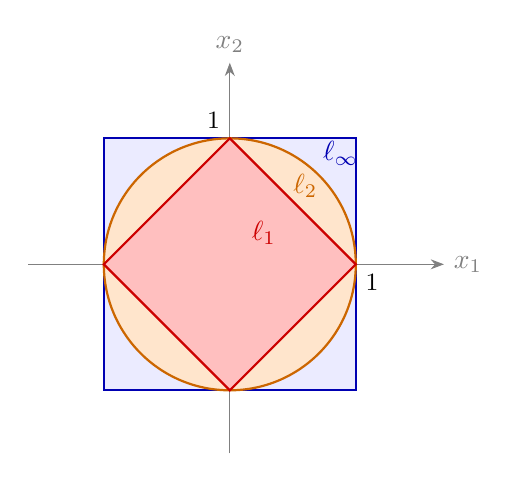
\begin{tikzpicture}[x=1.6cm, y=1.6cm, >=Stealth]
        \draw[->, gray] (-1.6,0) -- (1.7,0) node[right] {$x_1$};
        \draw[->, gray] (0,-1.5) -- (0,1.6) node[above] {$x_2$};
        \fill[blue!8] (-1,-1) -- (1,-1) -- (1,1) -- (-1,1) -- cycle;
        \fill[orange!20] (0,0) circle (1);
        \fill[red!25] (1,0) -- (0,1) -- (-1,0) -- (0,-1) -- cycle;
        \draw[blue!70!black, thick] (-1,-1) -- (1,-1) -- (1,1) -- (-1,1) -- cycle;
        \draw[orange!80!black, thick] (0,0) circle (1);
        \draw[red!80!black, thick] (1,0) -- (0,1) -- (-1,0) -- (0,-1) -- cycle;
        \node[red!80!black] at (0.27,0.25) {$\ell_1$};
        \node[orange!80!black] at (0.6,0.62) {$\ell_2$};
        \node[blue!70!black] at (0.88,0.88) {$\ell_\infty$};
        \node[below right] at (1,0) {\small $1$};
        \node[above left] at (0,1) {\small $1$};
    \end{tikzpicture}
    \caption[Unit balls of the $\ell_1$, $\ell_2$ and $\ell_\infty$ norms]{The unit balls $\{\mathbf{x} \in \mathbb{R}^2 : \norm{\mathbf{x}} \leq 1\}$ of the $\ell_1$ norm (red diamond), the $\ell_2$ norm (orange disk) and the $\ell_\infty$ norm (blue square). Each ball contains the previous one, in accordance with Proposition~\ref{L2-prop:norm-comparison}.}
    \label{L2-fig:unit-balls}
\end{figure}

\begin{proposition}\label{L2-prop:norm-comparison}
    For every $\mathbf{x} \in \mathbb{R}^n$,
    \[\norm{\mathbf{x}}_\infty \leq \norm{\mathbf{x}}_2 \leq \norm{\mathbf{x}}_1 \leq n \norm{\mathbf{x}}_\infty.\]
\end{proposition}

\begin{proof}
    Let $|x_k| = \norm{\mathbf{x}}_\infty$ be the largest absolute value of an entry of $\mathbf{x}$. Then $\norm{\mathbf{x}}_\infty^2 = x_k^2 \leq x_1^2 + \cdots + x_n^2 = \norm{\mathbf{x}}_2^2$. Next,
    \[\norm{\mathbf{x}}_1^2 = \Big(\sum_i |x_i|\Big)^2 = \sum_i x_i^2 + \sum_{i \neq j} |x_i| |x_j| \geq \sum_i x_i^2 = \norm{\mathbf{x}}_2^2.\]
    Finally, $\norm{\mathbf{x}}_1 = \sum_i |x_i| \leq \sum_i |x_k| = n \norm{\mathbf{x}}_\infty$.
\end{proof}

So all three norms are ``comparable'': if a vector is small in one of them, it is also small in the others (up to a factor that depends on $n$). In Example~\ref{L2-ex:l1-l2} we improve the last inequality.

\begin{example}[Frobenius norm]
    In Lecture~1, we saw that the space $\mathbb{R}^{m \times n}$ of $m \times n$ matrices is a vector space, and it is isomorphic to $\mathbb{R}^{mn}$ by listing the entries of a matrix. The Euclidean norm of this list of entries is the Frobenius norm
    \[\norm{A}_F = \sqrt{\sum_{i=1}^m \sum_{j=1}^n A_{ij}^2} = \sqrt{\tr(A^\top A)},\]
    which is a norm on $\mathbb{R}^{m \times n}$.
\end{example}

\begin{remark}[Norms in machine learning]
    Norms are used to measure the size of model parameters. In regularized linear regression, we minimize the error of a model plus a penalty $\lambda \norm{\mathbf{w}}$ on its weight vector $\mathbf{w}$. With the squared $\ell_2$ norm (ridge regression), all weights are shrunk towards $0$. With the $\ell_1$ norm (the lasso), many weights become exactly $0$, which gives sparse models; one reason is that the $\ell_1$ unit ball in Figure~\ref{L2-fig:unit-balls} has corners on the coordinate axes. The $\ell_\infty$ norm appears, for example, when we bound how much an adversary may change each pixel of an image.
\end{remark}

\section{Inner Products}

Norms measure lengths. To also measure angles, we need more structure: an inner product. The prototype is the dot product $\mathbf{x}^\top \mathbf{y}$ on $\mathbb{R}^n$.

\begin{definition}[Inner product]\label{L2-def:inner-product}
    Let $V$ be a vector space. A function $\ip{\cdot}{\cdot}: V \times V \to \mathbb{R}$ is called
    \begin{itemize}
        \item bilinear if it is linear in each argument: for all $x, y, z \in V$ and $\lambda, \mu \in \mathbb{R}$,
        \[\ip{\lambda x + \mu y}{z} = \lambda \ip{x}{z} + \mu \ip{y}{z} \qquad \text{and} \qquad \ip{z}{\lambda x + \mu y} = \lambda \ip{z}{x} + \mu \ip{z}{y};\]
        \item symmetric if $\ip{x}{y} = \ip{y}{x}$ for all $x, y \in V$;
        \item positive definite if $\ip{x}{x} > 0$ for all $x \in V$ with $x \neq 0$.
    \end{itemize}
    An inner product on $V$ is a positive definite, symmetric, bilinear function $V \times V \to \mathbb{R}$. A vector space together with an inner product is called an inner product space.
\end{definition}

Note that $\ip{0}{x} = \ip{0 \cdot 0}{x} = 0 \cdot \ip{0}{x} = 0$ by bilinearity, so in particular $\ip{0}{0} = 0$.

\begin{example}[Dot product]\label{L2-ex:dot}
    The dot product $\ip{\mathbf{x}}{\mathbf{y}} = \mathbf{x}^\top \mathbf{y} = \sum_i x_i y_i$ is an inner product on $\mathbb{R}^n$. It is bilinear and symmetric by the rules of matrix multiplication, and $\mathbf{x}^\top \mathbf{x} = x_1^2 + \cdots + x_n^2 > 0$ for $\mathbf{x} \neq \mathbf{0}$. The space $\mathbb{R}^n$ with the dot product is called the Euclidean space. Unless we say otherwise, we always use the dot product on $\mathbb{R}^n$.
\end{example}

\begin{example}\label{L2-ex:ip-A}
    On $\mathbb{R}^2$, define
    \[\ip{\mathbf{x}}{\mathbf{y}} = x_1 y_1 - (x_1 y_2 + x_2 y_1) + 2 x_2 y_2.\]
    This function is bilinear and symmetric. It is also positive definite, since
    \[\ip{\mathbf{x}}{\mathbf{x}} = x_1^2 - 2 x_1 x_2 + 2 x_2^2 = (x_1 - x_2)^2 + x_2^2 \geq 0,\]
    with equality only if $x_2 = 0$ and $x_1 = x_2$, i.e., $\mathbf{x} = \mathbf{0}$. So it is an inner product, different from the dot product: for example, for $\mathbf{x} = (1, 1)^\top$, we get $\ip{\mathbf{x}}{\mathbf{x}} = 1$, while $\mathbf{x}^\top \mathbf{x} = 2$.
\end{example}

\begin{example}
    \begin{itemize}
        \item For positive weights $w_1, \ldots, w_n > 0$, the weighted dot product $\ip{\mathbf{x}}{\mathbf{y}} = w_1 x_1 y_1 + \cdots + w_n x_n y_n$ is an inner product on $\mathbb{R}^n$. In machine learning, such weights can be used to make some features more important than others.
        \item The function $\ip{\mathbf{x}}{\mathbf{y}} = x_1 y_1 - x_2 y_2$ on $\mathbb{R}^2$ is bilinear and symmetric, but it is not an inner product, since $\ip{\mathbf{e}_2}{\mathbf{e}_2} = -1 < 0$.
        \item On the space $\mathbb{R}^{m \times n}$ of matrices, $\ip{A}{B} = \tr(A^\top B) = \sum_{i, j} A_{ij} B_{ij}$ is an inner product, the Frobenius inner product. It is the dot product of the lists of entries of $A$ and $B$.
    \end{itemize}
\end{example}

\subsection{Symmetric positive definite matrices}

All the inner products on $\mathbb{R}^n$ in the examples above can be written using a matrix. For instance, the inner product of Example~\ref{L2-ex:ip-A} is
\[\ip{\mathbf{x}}{\mathbf{y}} = \begin{pmatrix} x_1 & x_2 \end{pmatrix} \begin{pmatrix} 1 & -1 \\ -1 & 2 \end{pmatrix} \begin{pmatrix} y_1 \\ y_2 \end{pmatrix} = \mathbf{x}^\top A \mathbf{y}.\]
The matrices that give inner products in this way are the following.

\begin{definition}[Symmetric positive definite matrix]\label{L2-def:spd}
    A symmetric $n \times n$ matrix $A$ is called positive definite if
    \[\mathbf{x}^\top A \mathbf{x} > 0 \qquad \text{for all } \mathbf{x} \in \mathbb{R}^n \text{ with } \mathbf{x} \neq \mathbf{0},\]
    and positive semidefinite if $\mathbf{x}^\top A \mathbf{x} \geq 0$ for all $\mathbf{x} \in \mathbb{R}^n$. A symmetric positive definite matrix is also called an SPD matrix.
\end{definition}

\begin{theorem}\label{L2-thm:spd}
    \begin{enumerate}
        \item If $A$ is a symmetric positive definite $n \times n$ matrix, then $\ip{\mathbf{x}}{\mathbf{y}}_A = \mathbf{x}^\top A \mathbf{y}$ is an inner product on $\mathbb{R}^n$.
        \item Conversely, let $\ip{\cdot}{\cdot}$ be an inner product on an $n$-dimensional vector space $V$, and let $\mathcal{B} = (b_1, \ldots, b_n)$ be an ordered basis of $V$. Let $A$ be the $n \times n$ matrix with entries $A_{ij} = \ip{b_i}{b_j}$. Then $A$ is symmetric positive definite, and
        \[\ip{x}{y} = [x]_{\mathcal{B}}^\top \, A \, [y]_{\mathcal{B}} \qquad \text{for all } x, y \in V,\]
        where $[x]_{\mathcal{B}}$ is the coordinate vector of $x$ with respect to $\mathcal{B}$, as in Lecture~1.
    \end{enumerate}
\end{theorem}

\begin{proof}
    (1) The function $x^\top A y$ is bilinear by the distributivity of matrix multiplication and the rules for scalars. It is symmetric, since $y^\top A x$ is a $1 \times 1$ matrix and therefore equal to its transpose $(y^\top A x)^\top = x^\top A^\top y = x^\top A y$. It is positive definite by assumption.

    (2) Write $x = \sum_i \psi_i b_i$ and $y = \sum_j \lambda_j b_j$, so that $[x]_{\mathcal{B}} = (\psi_1, \ldots, \psi_n)^\top$ and $[y]_{\mathcal{B}} = (\lambda_1, \ldots, \lambda_n)^\top$. By bilinearity,
    \[\ip{x}{y} = \Big\langle \sum_i \psi_i b_i, \sum_j \lambda_j b_j \Big\rangle = \sum_{i, j} \psi_i \ip{b_i}{b_j} \lambda_j = [x]_{\mathcal{B}}^\top A [y]_{\mathcal{B}}.\]
    The matrix $A$ is symmetric, since $\ip{b_i}{b_j} = \ip{b_j}{b_i}$. If $\boldsymbol{\psi} \in \mathbb{R}^n$ is nonzero, then $x = \sum_i \psi_i b_i \neq 0$, since the $b_i$ are linearly independent, and hence $\boldsymbol{\psi}^\top A \boldsymbol{\psi} =\ip{x}{x} > 0$.
\end{proof}

The matrix $A$ in part 2 is called the Gram matrix of the basis $\mathcal{B}$. So, once we fix a basis, inner products on an $n$-dimensional space are the same thing as symmetric positive definite $n \times n$ matrices. The dot product on $\mathbb{R}^n$ corresponds to $A = I_n$ and the standard basis.

\begin{proposition}\label{L2-prop:spd-properties}
    Let $A$ be a symmetric positive definite $n \times n$ matrix.
    \begin{enumerate}
        \item The diagonal entries of $A$ are positive.
        \item $A$ is invertible.
        \item For $n = 2$: a symmetric matrix $A = \begin{pmatrix} a & b \\ b & c \end{pmatrix}$ is positive definite if and only if $a > 0$ and $\det(A) = ac - b^2 > 0$.
    \end{enumerate}
\end{proposition}

\begin{proof}
    (1) $A_{ii} = \mathbf{e}_i^\top A \mathbf{e}_i > 0$.

    (2) If $A\mathbf{x} = \mathbf{0}$, then $\mathbf{x}^\top A \mathbf{x} = 0$, so $\mathbf{x} = \mathbf{0}$. Hence $\Null(A) = \{\mathbf{0}\}$, and $A$ is invertible by Lecture~1.

    (3) If $A$ is positive definite, then $a > 0$ by part 1. If $a > 0$, completing the square gives
    \[\mathbf{x}^\top A \mathbf{x} = a x_1^2 + 2b x_1 x_2 + c x_2^2 = a \Big(x_1 + \frac{b}{a} x_2\Big)^2 + \frac{ac - b^2}{a} x_2^2.\]
    If $ac - b^2 > 0$, both terms are nonnegative, and they are both zero only if $x_2 = 0$ and $x_1 = 0$; so $A$ is positive definite. If $ac - b^2 \leq 0$, then $\mathbf{x} = (-b, a)^\top \neq \mathbf{0}$ gives $\mathbf{x}^\top A \mathbf{x} = (ac - b^2) a \leq 0$, so $A$ is not positive definite.
\end{proof}

For larger matrices, there is a similar test, Sylvester's criterion: a symmetric matrix is positive definite if and only if the determinants of all its upper left $k \times k$ submatrices, for $k = 1, \ldots, n$, are positive. We prove it in Section~\ref{L2-sec:spectral} (Corollary~\ref{L2-cor:sylvester}), together with another test, using eigenvalues (Corollary~\ref{L2-cor:spd-eigenvalues}).

\begin{example}
    The matrix $A_1 = \begin{pmatrix} 9 & 6 \\ 6 & 5 \end{pmatrix}$ is positive definite, since $9 > 0$ and $\det(A_1) = 45 - 36 = 9 > 0$. Indeed, $\mathbf{x}^\top A_1 \mathbf{x} = (3x_1 + 2x_2)^2 + x_2^2$. The matrix $A_2 = \begin{pmatrix} 9 & 6 \\ 6 & 3 \end{pmatrix}$ is not, since $\det(A_2) = 27 - 36 = -9 < 0$: for $\mathbf{x} = (2, -3)^\top$, we get $\mathbf{x}^\top A_2 \mathbf{x} = -9$.
\end{example}

\begin{example}\label{L2-ex:BTB}
    Let $B$ be an $m \times n$ matrix with linearly independent columns. Then $B^\top B$ is symmetric positive definite: it is symmetric (Lecture~1), and for $\mathbf{x} \neq \mathbf{0}$ we have $B\mathbf{x} \neq \mathbf{0}$, so
    \[\mathbf{x}^\top B^\top B \mathbf{x} = (B\mathbf{x})^\top (B\mathbf{x}) = \norm{B\mathbf{x}}_2^2 > 0.\]
    Matrices of the form $B^\top B$ appear everywhere in machine learning, for example in linear regression (Section~\ref{L2-sec:least-squares}) and as (scaled) covariance matrices of data.
\end{example}

\begin{remark}[Kernels]
    Many machine learning methods, such as support vector machines, only use the data through inner products $\ip{\mathbf{x}_i}{\mathbf{x}_j}$ of data points. Kernel methods replace them by $k(\mathbf{x}_i, \mathbf{x}_j) = \ip{\phi(\mathbf{x}_i)}{\phi(\mathbf{x}_j)}$, the inner product of the data after a (possibly nonlinear) feature map $\phi$. The matrix $K$ with entries $K_{ij} = k(\mathbf{x}_i, \mathbf{x}_j)$ is then a Gram matrix, and it is symmetric positive semidefinite.
\end{remark}

\section{Lengths and Distances}\label{L2-sec:lengths}

\subsection{The norm of an inner product}

Every inner product gives a norm, in the same way that the dot product gives the Euclidean norm $\norm{\mathbf{x}}_2 = \sqrt{\mathbf{x}^\top \mathbf{x}}$.

\begin{definition}[Induced norm]
    Let $V$ be an inner product space. The length, or norm, of a vector $x \in V$ is
    \[\norm{x} = \sqrt{\ip{x}{x}}.\]
    A vector $x$ with $\norm{x} = 1$ is called a unit vector. For $x \neq 0$, the vector $\frac{x}{\norm{x}}$ is a unit vector; replacing $x$ by $\frac{x}{\norm{x}}$ is called normalizing $x$.
\end{definition}

\begin{example}
    For $\mathbf{x} = (1, 1)^\top$, the dot product gives $\norm{\mathbf{x}} = \sqrt{2}$, while the inner product of Example~\ref{L2-ex:ip-A} gives $\norm{\mathbf{x}} = \sqrt{1} = 1$. So the length of a vector depends on the choice of the inner product.
\end{example}

To show that $\norm{x} = \sqrt{\ip{x}{x}}$ really is a norm, we need the most important inequality of linear algebra.

\begin{theorem}[Cauchy--Schwarz inequality]\label{L2-thm:cauchy-schwarz}
    Let $V$ be an inner product space. For all $x, y \in V$,
    \[|\ip{x}{y}| \leq \norm{x} \, \norm{y},\]
    with equality if and only if $x$ and $y$ are linearly dependent.
\end{theorem}

\begin{proof}
    If $y = 0$, both sides are $0$, and $x$, $y$ are linearly dependent. So let $y \neq 0$. For every $t \in \mathbb{R}$, by bilinearity and symmetry,
    \[0 \leq \ip{x - ty}{x - ty} = \norm{x}^2 - 2t \ip{x}{y} + t^2 \norm{y}^2.\]
    Choosing $t = \frac{\ip{x}{y}}{\norm{y}^2}$ gives
    \[0 \leq \norm{x}^2 - 2\frac{\ip{x}{y}^2}{\norm{y}^2} + \frac{\ip{x}{y}^2}{\norm{y}^2} = \norm{x}^2 - \frac{\ip{x}{y}^2}{\norm{y}^2},\]
    i.e., $\ip{x}{y}^2 \leq \norm{x}^2 \norm{y}^2$. Taking square roots proves the inequality. Equality holds if and only if $\ip{x - ty}{x - ty} = 0$ for this $t$, i.e., $x = ty$, which (for $y \neq 0$) means that $x$ and $y$ are linearly dependent.
\end{proof}

\begin{corollary}\label{L2-cor:induced-norm}
    If $V$ is an inner product space, then $\norm{x} = \sqrt{\ip{x}{x}}$ is a norm on $V$. In particular, the Euclidean norm $\norm{\cdot}_2$ is a norm on $\mathbb{R}^n$.
\end{corollary}

\begin{proof}
    Positive definiteness follows from the positive definiteness of the inner product, and $\norm{\lambda x} = \sqrt{\lambda^2 \ip{x}{x}} = |\lambda| \norm{x}$. For the triangle inequality, by the Cauchy--Schwarz inequality,
    \[\norm{x + y}^2 = \norm{x}^2 + 2 \ip{x}{y} + \norm{y}^2 \leq \norm{x}^2 + 2 \norm{x} \norm{y} + \norm{y}^2 = \big(\norm{x} + \norm{y}\big)^2. \qedhere\]
\end{proof}

\begin{example}\label{L2-ex:l1-l2}
    Let $\mathbf{a} = (|x_1|, \ldots, |x_n|)^\top$ and $\mathbf{1} = (1, \ldots, 1)^\top$. Applying the Cauchy--Schwarz inequality for the dot product to $\mathbf{a}$ and $\mathbf{1}$ gives
    \[\norm{\mathbf{x}}_1 = \sum_{i=1}^n |x_i| \cdot 1 \leq \sqrt{\sum_{i=1}^n x_i^2} \, \sqrt{\sum_{i=1}^n 1^2} = \sqrt{n} \, \norm{\mathbf{x}}_2.\]
    This improves the inequality $\norm{\mathbf{x}}_1 \leq n \norm{\mathbf{x}}_\infty$ of Proposition~\ref{L2-prop:norm-comparison}, since $\sqrt{n} \norm{\mathbf{x}}_2 \leq n \norm{\mathbf{x}}_\infty$.
\end{example}

Not every norm comes from an inner product. Norms that do come from an inner product can be recognized by the following identities.

\begin{proposition}[Parallelogram law and polarization]\label{L2-prop:parallelogram}
    Let $V$ be an inner product space with the induced norm. For all $x, y \in V$:
    \begin{enumerate}
        \item $\norm{x + y}^2 + \norm{x - y}^2 = 2\norm{x}^2 + 2\norm{y}^2$ (parallelogram law);
        \item $\ip{x}{y} = \frac{1}{4}\big(\norm{x + y}^2 - \norm{x - y}^2\big)$ (polarization identity).
    \end{enumerate}
\end{proposition}

\begin{proof}
    Expanding with bilinearity, $\norm{x \pm y}^2 = \norm{x}^2 \pm 2\ip{x}{y} + \norm{y}^2$. Adding the two identities gives part 1; subtracting them gives part 2.
\end{proof}

The parallelogram law says that in a parallelogram, the sum of the squares of the two diagonals equals the sum of the squares of the four sides. The polarization identity shows that the inner product can be recovered from its norm.

\begin{example}
    The $\ell_1$ norm on $\mathbb{R}^2$ does not come from any inner product: for $\mathbf{x} = \mathbf{e}_1$ and $\mathbf{y} = \mathbf{e}_2$, we get $\norm{\mathbf{x} + \mathbf{y}}_1^2 + \norm{\mathbf{x} - \mathbf{y}}_1^2 = 4 + 4 = 8$, but $2\norm{\mathbf{x}}_1^2 + 2\norm{\mathbf{y}}_1^2 = 4$, so the parallelogram law fails. Hence normed spaces are more general than inner product spaces.
\end{example}

\subsection{Distances}

\begin{definition}[Distance]
    Let $V$ be an inner product space (or, more generally, a normed space). The distance between $x, y \in V$ is
    \[d(x, y) = \norm{x - y}.\]
    For the dot product on $\mathbb{R}^n$, this is the Euclidean distance $d(\mathbf{x}, \mathbf{y}) = \norm{\mathbf{x} - \mathbf{y}}_2 = \sqrt{\sum_i (x_i - y_i)^2}$.
\end{definition}

\begin{proposition}\label{L2-prop:metric}
    The distance $d$ has the following properties, for all $x, y, z \in V$:
    \begin{enumerate}
        \item Positive definiteness: $d(x, y) \geq 0$, and $d(x, y) = 0$ if and only if $x = y$;
        \item Symmetry: $d(x, y) = d(y, x)$;
        \item Triangle inequality: $d(x, z) \leq d(x, y) + d(y, z)$.
    \end{enumerate}
\end{proposition}

\begin{proof}
    Part 1 follows from the positive definiteness of the norm, and part 2 from $\norm{x - y} = \norm{(-1)(y - x)} = \norm{y - x}$. Part 3 is the triangle inequality for the norm, applied to $x - z = (x - y) + (y - z)$.
\end{proof}

A function $d: X \times X \to \mathbb{R}$ on any set $X$ with these three properties is called a metric, and $(X, d)$ is called a metric space. So every normed space is a metric space.

\begin{example}
    For $\mathbf{x} = (1, 2)^\top$ and $\mathbf{y} = (4, 6)^\top$, we have $\mathbf{x} - \mathbf{y} = (-3, -4)^\top$, so the distance between $\mathbf{x}$ and $\mathbf{y}$ is
    \[\norm{\mathbf{x} - \mathbf{y}}_2 = \sqrt{9 + 16} = 5, \qquad \norm{\mathbf{x} - \mathbf{y}}_1 = 3 + 4 = 7, \qquad \norm{\mathbf{x} - \mathbf{y}}_\infty = 4\]
    for the Euclidean, Manhattan and maximum norms, respectively.
\end{example}

\begin{remark}[Distances in machine learning]
    The $k$-nearest neighbor method classifies a new data point by a majority vote among the $k$ training points that are closest to it. Which points are closest depends on the metric, so the choice of the norm matters. It also depends on the units of the features: if one feature is measured in meters and another in millimeters, the second one dominates the Euclidean distance. This is why features are usually standardized first, or, equivalently, a weighted inner product is used.
\end{remark}

\section{Angles and Orthogonality}

\subsection{Angles}

By the Cauchy--Schwarz inequality, $-1 \leq \frac{\ip{x}{y}}{\norm{x} \norm{y}} \leq 1$ for nonzero vectors $x$ and $y$. So the following definition makes sense.

\begin{definition}[Angle]
    Let $V$ be an inner product space, and let $x, y \in V$ be nonzero. The angle between $x$ and $y$ is the unique number $\omega \in [0, \pi]$ with
    \[\cos \omega = \frac{\ip{x}{y}}{\norm{x} \, \norm{y}}.\]
\end{definition}

For the dot product in $\mathbb{R}^2$ or $\mathbb{R}^3$, this is the usual angle between two arrows. Indeed, expanding $\norm{\mathbf{x} - \mathbf{y}}^2$ gives
\[\norm{\mathbf{x} - \mathbf{y}}^2 = \norm{\mathbf{x}}^2 + \norm{\mathbf{y}}^2 - 2 \ip{\mathbf{x}}{\mathbf{y}} = \norm{\mathbf{x}}^2 + \norm{\mathbf{y}}^2 - 2 \norm{\mathbf{x}} \norm{\mathbf{y}} \cos\omega,\]
which is the law of cosines for the triangle with sides $\mathbf{x}$, $\mathbf{y}$ and $\mathbf{x} - \mathbf{y}$ (see Figure~\ref{L2-fig:angle}).

\begin{example}\label{L2-ex:angle}
    The angle $\omega$ between $\mathbf{x} = (3, 1)^\top$ and $\mathbf{y} = (1, 2)^\top$ satisfies
    \[\cos\omega = \frac{3 \cdot 1 + 1 \cdot 2}{\sqrt{10} \, \sqrt{5}} = \frac{5}{\sqrt{50}} = \frac{1}{\sqrt{2}},\]
    so $\omega = \frac{\pi}{4}$, i.e., $45^\circ$.
\end{example}

\begin{figure}[ht]
    \centering
    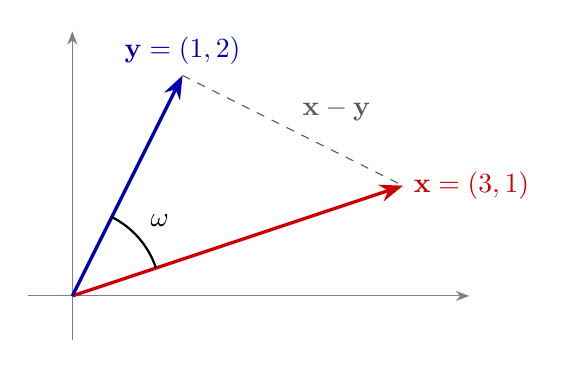
\begin{tikzpicture}[x=1.4cm, y=1.4cm, >=Stealth]
        \draw[->, gray] (-0.4,0) -- (3.6,0);
        \draw[->, gray] (0,-0.4) -- (0,2.4);
        \draw[->, very thick, red!80!black] (0,0) -- (3,1) node[right] {$\mathbf{x} = (3, 1)$};
        \draw[->, very thick, blue!70!black] (0,0) -- (1,2) node[above] {$\mathbf{y} = (1, 2)$};
        \draw[dashed, gray!70!black] (1,2) -- node[above right] {$\mathbf{x} - \mathbf{y}$} (3,1);
        \draw[thick] (18.43:0.8) arc[start angle=18.43, end angle=63.43, radius=0.8];
        \node at (40.93:1.05) {$\omega$};
    \end{tikzpicture}
    \caption[The angle between two vectors]{The angle $\omega = 45^\circ$ between $\mathbf{x} = (3, 1)$ and $\mathbf{y} = (1, 2)$ (Example~\ref{L2-ex:angle}). The triangle with sides $\mathbf{x}$, $\mathbf{y}$ and $\mathbf{x} - \mathbf{y}$ satisfies the law of cosines.}
    \label{L2-fig:angle}
\end{figure}

\subsection{Orthogonality}

\begin{definition}[Orthogonality]
    Two vectors $x$ and $y$ of an inner product space are orthogonal, written $x \perp y$, if $\ip{x}{y} = 0$. If, in addition, $\norm{x} = \norm{y} = 1$, then $x$ and $y$ are called orthonormal.
\end{definition}

So two nonzero vectors are orthogonal if and only if the angle between them is $\frac{\pi}{2}$. The zero vector is orthogonal to every vector.

\begin{example}\label{L2-ex:orth-depends}
    The vectors $\mathbf{x} = (1, 1)^\top$ and $\mathbf{y} = (-1, 1)^\top$ are orthogonal for the dot product, since $\mathbf{x}^\top \mathbf{y} = -1 + 1 = 0$. Now consider the inner product $\ip{\mathbf{x}}{\mathbf{y}} = \mathbf{x}^\top A \mathbf{y}$ with $A = \diag(2, 1)$. Then
    \[\ip{\mathbf{x}}{\mathbf{y}} = 2 \cdot 1 \cdot (-1) + 1 \cdot 1 = -1, \qquad \norm{\mathbf{x}}^2 = 2 + 1 = 3, \qquad \norm{\mathbf{y}}^2 = 2 + 1 = 3,\]
    so $\cos\omega = -\frac{1}{3}$ and $\omega \approx 1.91 \approx 109.5^\circ$. So whether two vectors are orthogonal depends on the inner product.
\end{example}

\begin{theorem}[Pythagoras]\label{L2-thm:pythagoras}
    If $x \perp y$, then $\norm{x + y}^2 = \norm{x}^2 + \norm{y}^2$.
\end{theorem}

\begin{proof}
    $\norm{x + y}^2 = \norm{x}^2 + 2\ip{x}{y} + \norm{y}^2 = \norm{x}^2 + \norm{y}^2$.
\end{proof}

\begin{remark}[Cosine similarity]
    In machine learning, the number $\cos\omega = \frac{\ip{\mathbf{x}}{\mathbf{y}}}{\norm{\mathbf{x}} \norm{\mathbf{y}}}$ is called the cosine similarity of $\mathbf{x}$ and $\mathbf{y}$. It is $1$ if $\mathbf{x}$ and $\mathbf{y}$ point in the same direction, $0$ if they are orthogonal, and $-1$ if they point in opposite directions. Unlike the distance, it does not change when $\mathbf{x}$ or $\mathbf{y}$ is multiplied by a positive scalar. This makes it useful for comparing text documents (represented by word counts, where long and short documents should be comparable) and embeddings, e.g., the vectors that language models assign to words and sentences.
\end{remark}

\subsection{Orthogonal matrices}

In Lecture~1, we defined an $n \times n$ matrix $Q$ to be orthogonal if $Q^\top Q = I_n$, and we claimed that orthogonal matrices preserve lengths and angles. We can now make this precise and prove it.

\begin{theorem}\label{L2-thm:orthogonal}
    For an $n \times n$ matrix $Q$, the following statements are equivalent:
    \begin{enumerate}
        \item $Q$ is orthogonal, i.e., $Q^\top Q = I_n$;
        \item $Q$ preserves the dot product: $(Q\mathbf{x})^\top (Q\mathbf{y}) = \mathbf{x}^\top \mathbf{y}$ for all $\mathbf{x}, \mathbf{y} \in \mathbb{R}^n$;
        \item $Q$ preserves lengths: $\norm{Q\mathbf{x}}_2 = \norm{\mathbf{x}}_2$ for all $\mathbf{x} \in \mathbb{R}^n$;
        \item the columns of $Q$ are orthonormal.
    \end{enumerate}
    In particular, orthogonal matrices preserve lengths, distances and angles.
\end{theorem}

\begin{proof}
    ($1 \Rightarrow 2$) $(Q\mathbf{x})^\top (Q\mathbf{y}) = \mathbf{x}^\top Q^\top Q \mathbf{y} = \mathbf{x}^\top \mathbf{y}$.

    ($2 \Rightarrow 3$) Take $\mathbf{y} = \mathbf{x}$ and take square roots.

    ($3 \Rightarrow 2$) By the polarization identity (Proposition~\ref{L2-prop:parallelogram}) and linearity,
    \[(Q\mathbf{x})^\top (Q\mathbf{y}) = \tfrac{1}{4}\big(\norm{Q\mathbf{x} + Q\mathbf{y}}^2 - \norm{Q\mathbf{x} - Q\mathbf{y}}^2\big) = \tfrac{1}{4}\big(\norm{\mathbf{x} + \mathbf{y}}^2 - \norm{\mathbf{x} - \mathbf{y}}^2\big) = \mathbf{x}^\top \mathbf{y}.\]

    ($2 \Rightarrow 1$) The $(i, j)$ entry of $Q^\top Q$ is $\mathbf{e}_i^\top Q^\top Q \mathbf{e}_j = (Q\mathbf{e}_i)^\top (Q\mathbf{e}_j) = \mathbf{e}_i^\top \mathbf{e}_j$, which is $1$ if $i = j$ and $0$ otherwise.

    ($1 \Leftrightarrow 4$) The $(i, j)$ entry of $Q^\top Q$ is $\mathbf{q}_i^\top \mathbf{q}_j$, where $\mathbf{q}_1, \ldots, \mathbf{q}_n$ are the columns of $Q$. So $Q^\top Q = I_n$ means exactly that $\mathbf{q}_i^\top \mathbf{q}_j$ is $1$ for $i = j$ and $0$ for $i \neq j$.

    Finally, distances are lengths of differences, $\norm{Q\mathbf{x} - Q\mathbf{y}}_2 = \norm{Q(\mathbf{x} - \mathbf{y})}_2 = \norm{\mathbf{x} - \mathbf{y}}_2$, and angles are defined in terms of the dot product and lengths.
\end{proof}

A map that preserves distances is called an isometry. Rotations and reflections are the typical examples; we study rotations in Section~\ref{L2-sec:rotations}.

\section{Orthonormal Bases}

In $\mathbb{R}^n$, the standard basis $\mathbf{e}_1, \ldots, \mathbf{e}_n$ consists of vectors of length $1$ that are pairwise orthogonal. Bases with this property are especially convenient.

\begin{definition}[Orthonormal basis]
    Let $V$ be an inner product space. Vectors $b_1, \ldots, b_k \in V$ are called orthogonal if $\ip{b_i}{b_j} = 0$ for all $i \neq j$, and orthonormal if, in addition, $\norm{b_i} = 1$ for all $i$. In other words, $b_1, \ldots, b_k$ are orthonormal if
    \[\ip{b_i}{b_j} = \begin{cases} 1 & \text{if } i = j, \\ 0 & \text{if } i \neq j. \end{cases}\]
    An orthonormal basis (ONB) of $V$ is a basis of $V$ consisting of orthonormal vectors.
\end{definition}

\begin{lemma}\label{L2-lem:orth-indep}
    Orthogonal nonzero vectors $b_1, \ldots, b_k$ are linearly independent.
\end{lemma}

\begin{proof}
    Suppose that $a_1 b_1 + \cdots + a_k b_k = 0$. Taking the inner product with $b_j$ and using bilinearity gives
    \[0 = \ip{a_1 b_1 + \cdots + a_k b_k}{b_j} = a_1 \ip{b_1}{b_j} + \cdots + a_k \ip{b_k}{b_j} = a_j \norm{b_j}^2.\]
    Since $b_j \neq 0$, we get $a_j = 0$, for every $j$.
\end{proof}

The main advantage of an orthonormal basis is that coordinates are computed by inner products, without solving a system of linear equations.

\begin{proposition}\label{L2-prop:onb-coordinates}
    Let $b_1, \ldots, b_n$ be an orthonormal basis of $V$. Then for all $u, v \in V$:
    \begin{enumerate}
        \item $v = \ip{v}{b_1} b_1 + \ip{v}{b_2} b_2 + \cdots + \ip{v}{b_n} b_n$;
        \item $\ip{u}{v} = \sum_{i=1}^n \ip{u}{b_i} \ip{v}{b_i}$, and in particular $\norm{v}^2 = \sum_{i=1}^n \ip{v}{b_i}^2$ (Parseval's identity).
    \end{enumerate}
\end{proposition}

\begin{proof}
    (1) Write $v = c_1 b_1 + \cdots + c_n b_n$. Taking the inner product with $b_j$ gives $\ip{v}{b_j} = \sum_i c_i \ip{b_i}{b_j} = c_j$.

    (2) Write $u = \sum_i d_i b_i$ and $v = \sum_j c_j b_j$ with $d_i = \ip{u}{b_i}$ and $c_j = \ip{v}{b_j}$. Then $\ip{u}{v} = \sum_{i, j} d_i c_j \ip{b_i}{b_j} = \sum_i d_i c_i$.
\end{proof}

In the language of Theorem~\ref{L2-thm:spd}: the Gram matrix of an orthonormal basis is the identity matrix, so in coordinates with respect to an orthonormal basis, every inner product becomes the dot product.

\begin{example}\label{L2-ex:onb-r2}
    The vectors $\mathbf{b}_1 = \frac{1}{\sqrt{2}}(1, 1)^\top$ and $\mathbf{b}_2 = \frac{1}{\sqrt{2}}(1, -1)^\top$ form an orthonormal basis of $\mathbb{R}^2$. For $\mathbf{v} = (3, 1)^\top$, we get
    \[\ip{\mathbf{v}}{\mathbf{b}_1} = \frac{4}{\sqrt{2}} = 2\sqrt{2}, \qquad \ip{\mathbf{v}}{\mathbf{b}_2} = \frac{2}{\sqrt{2}} = \sqrt{2},\]
    so $\mathbf{v} = 2\sqrt{2}\, \mathbf{b}_1 + \sqrt{2}\, \mathbf{b}_2 = 2(1, 1)^\top + (1, -1)^\top$. Parseval's identity checks out: $(2\sqrt{2})^2 + (\sqrt{2})^2 = 10 = 3^2 + 1^2$.
\end{example}

\begin{remark}
    If $\mathbf{b}_1, \ldots, \mathbf{b}_n$ is an orthonormal basis of $\mathbb{R}^n$ (with the dot product), then the matrix $Q$ with columns $\mathbf{b}_1, \ldots, \mathbf{b}_n$ is orthogonal (Theorem~\ref{L2-thm:orthogonal}). The coordinate vector of $\mathbf{v}$ is then $Q^{-1} \mathbf{v} = Q^\top \mathbf{v} = (\mathbf{b}_1^\top \mathbf{v}, \ldots, \mathbf{b}_n^\top \mathbf{v})^\top$, in agreement with Proposition~\ref{L2-prop:onb-coordinates}.
\end{remark}

\subsection{The Gram--Schmidt process}

Every basis can be turned into an orthonormal basis. The idea is to go through the basis vectors one by one, and to subtract from each vector its components in the directions of the previous ones.

\begin{theorem}[Gram--Schmidt process]\label{L2-thm:gram-schmidt}
    Let $v_1, \ldots, v_k$ be linearly independent vectors in an inner product space $V$. Define recursively, for $j = 1, \ldots, k$,
    \[u_j = v_j - \sum_{i=1}^{j-1} \ip{v_j}{e_i}\, e_i, \qquad e_j = \frac{u_j}{\norm{u_j}}.\]
    Then $e_1, \ldots, e_k$ are orthonormal, and $\Span\{e_1, \ldots, e_j\} = \Span\{v_1, \ldots, v_j\}$ for every $j = 1, \ldots, k$.
\end{theorem}

\begin{proof}
    We use induction on $j$. For $j = 1$, we have $u_1 = v_1 \neq 0$ and $e_1 = v_1 / \norm{v_1}$, so the claim holds. Now let $j \geq 2$, and assume that $e_1, \ldots, e_{j-1}$ are orthonormal with $\Span\{e_1, \ldots, e_{j-1}\} = \Span\{v_1, \ldots, v_{j-1}\}$.

    First, $u_j \neq 0$: otherwise $v_j = \sum_{i < j} \ip{v_j}{e_i} e_i$ would lie in $\Span\{e_1, \ldots, e_{j-1}\}$, which equals $\Span\{v_1, \ldots, v_{j-1}\}$, contradicting the linear independence of $v_1, \ldots, v_j$. So $e_j$ is well defined and has length $1$.

    Next, for $l < j$, using that $e_1, \ldots, e_{j-1}$ are orthonormal,
    \[\ip{u_j}{e_l} = \ip{v_j}{e_l} - \sum_{i < j} \ip{v_j}{e_i} \ip{e_i}{e_l} = \ip{v_j}{e_l} - \ip{v_j}{e_l} = 0,\]
    so $e_j$ is orthogonal to $e_1, \ldots, e_{j-1}$. Finally, $e_j$ is a linear combination of $v_j$ and $e_1, \ldots, e_{j-1}$, and conversely $v_j = \norm{u_j} e_j + \sum_{i < j} \ip{v_j}{e_i} e_i$. Together with the induction hypothesis, this gives $\Span\{e_1, \ldots, e_j\} = \Span\{v_1, \ldots, v_j\}$.
\end{proof}

The vector $\ip{v_j}{e_i} e_i$ is the component of $v_j$ in the direction of $e_i$; in Section~\ref{L2-sec:projections}, we will call it the orthogonal projection of $v_j$ onto $\Span\{e_i\}$. In hand computations, it is often easier to postpone the normalization: since $\ip{v_j}{e_i} e_i = \frac{\ip{v_j}{u_i}}{\ip{u_i}{u_i}} u_i$, the vectors
\[u_j = v_j - \sum_{i=1}^{j-1} \frac{\ip{v_j}{u_i}}{\ip{u_i}{u_i}}\, u_i\]
are orthogonal, and we normalize them at the end. Figure~\ref{L2-fig:gram-schmidt} illustrates the process for two vectors.

\begin{figure}[ht]
    \centering
    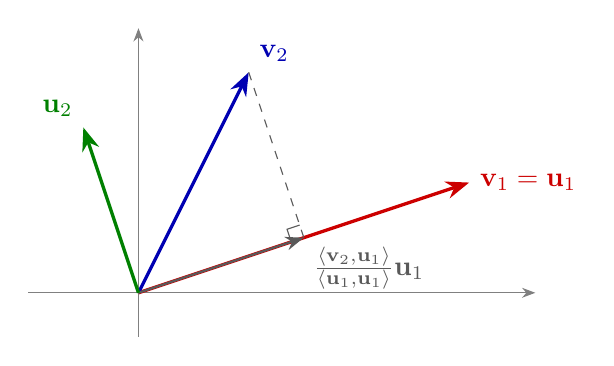
\begin{tikzpicture}[x=1.4cm, y=1.4cm, >=Stealth]
        \draw[->, gray] (-1,0) -- (3.6,0);
        \draw[->, gray] (0,-0.4) -- (0,2.4);
        \draw[->, very thick, red!80!black] (0,0) -- (3,1) node[right] {$\mathbf{v}_1 = \mathbf{u}_1$};
        \draw[->, very thick, blue!70!black] (0,0) -- (1,2) node[above right] {$\mathbf{v}_2$};
        \draw[->, thick, gray!70!black] (0,0) -- (1.5,0.5);
        \node[below right, gray!70!black] at (1.5,0.5) {$\frac{\langle \mathbf{v}_2, \mathbf{u}_1 \rangle}{\langle \mathbf{u}_1, \mathbf{u}_1 \rangle} \mathbf{u}_1$};
        \draw[dashed, gray!70!black] (1.5,0.5) -- (1,2);
        \draw[->, very thick, green!50!black] (0,0) -- (-0.5,1.5) node[above left] {$\mathbf{u}_2$};
        \draw[gray!70!black] (1.386,0.462) -- (1.348,0.576) -- (1.462,0.614);
    \end{tikzpicture}
    \caption[The Gram--Schmidt process]{The Gram--Schmidt process for $\mathbf{v}_1 = (3, 1)$ and $\mathbf{v}_2 = (1, 2)$. The component of $\mathbf{v}_2$ in the direction of $\mathbf{u}_1 = \mathbf{v}_1$ is $\frac{5}{10} \mathbf{u}_1 = (1.5, 0.5)$; subtracting it gives $\mathbf{u}_2 = (-0.5, 1.5)$, which is orthogonal to $\mathbf{u}_1$. Normalizing $\mathbf{u}_1$ and $\mathbf{u}_2$ gives an orthonormal basis of $\mathbb{R}^2$.}
    \label{L2-fig:gram-schmidt}
\end{figure}

\begin{example}\label{L2-ex:gram-schmidt}
    Let us apply the Gram--Schmidt process to the basis $\mathbf{v}_1 = (1, 1, 0)^\top$, $\mathbf{v}_2 = (1, 0, 1)^\top$, $\mathbf{v}_3 = (0, 1, 1)^\top$ of $\mathbb{R}^3$, using the unnormalized version:
    \begin{align*}
        \mathbf{u}_1 &= \mathbf{v}_1 = (1, 1, 0)^\top, \\
        \mathbf{u}_2 &= \mathbf{v}_2 - \frac{\mathbf{v}_2^\top \mathbf{u}_1}{\mathbf{u}_1^\top \mathbf{u}_1} \mathbf{u}_1 = (1, 0, 1)^\top - \frac{1}{2}(1, 1, 0)^\top = \big(\tfrac{1}{2}, -\tfrac{1}{2}, 1\big)^\top, \\
        \mathbf{u}_3 &= \mathbf{v}_3 - \frac{\mathbf{v}_3^\top \mathbf{u}_1}{\mathbf{u}_1^\top \mathbf{u}_1} \mathbf{u}_1 - \frac{\mathbf{v}_3^\top \mathbf{u}_2}{\mathbf{u}_2^\top \mathbf{u}_2} \mathbf{u}_2 = (0, 1, 1)^\top - \frac{1}{2}(1, 1, 0)^\top - \frac{1/2}{3/2}\big(\tfrac{1}{2}, -\tfrac{1}{2}, 1\big)^\top = \big(-\tfrac{2}{3}, \tfrac{2}{3}, \tfrac{2}{3}\big)^\top.
    \end{align*}
    One checks that $\mathbf{u}_1^\top \mathbf{u}_2 = \mathbf{u}_1^\top \mathbf{u}_3 = \mathbf{u}_2^\top \mathbf{u}_3 = 0$. Normalizing gives the orthonormal basis
    \[\mathbf{e}_1 = \frac{1}{\sqrt{2}} \begin{pmatrix} 1 \\ 1 \\ 0 \end{pmatrix}, \qquad \mathbf{e}_2 = \frac{1}{\sqrt{6}} \begin{pmatrix} 1 \\ -1 \\ 2 \end{pmatrix}, \qquad \mathbf{e}_3 = \frac{1}{\sqrt{3}} \begin{pmatrix} -1 \\ 1 \\ 1 \end{pmatrix}.\]
\end{example}

\begin{corollary}\label{L2-cor:onb-exists}
    Every finite-dimensional inner product space has an orthonormal basis.
\end{corollary}

\begin{proof}
    Apply the Gram--Schmidt process to any basis $v_1, \ldots, v_n$. The resulting vectors $e_1, \ldots, e_n$ are orthonormal and span $\Span\{v_1, \ldots, v_n\} = V$, and they are linearly independent by Lemma~\ref{L2-lem:orth-indep}.
\end{proof}

The Gram--Schmidt process can also be written as a factorization of matrices.

\begin{proposition}[QR decomposition]\label{L2-prop:qr}
    Let $A$ be an $m \times n$ matrix with linearly independent columns $\mathbf{a}_1, \ldots, \mathbf{a}_n$. Then $A = QR$, where $Q$ is an $m \times n$ matrix with orthonormal columns (i.e., $Q^\top Q = I_n$), and $R$ is an upper triangular $n \times n$ matrix with positive diagonal entries.
\end{proposition}

\begin{proof}
    Apply the Gram--Schmidt process to $\mathbf{a}_1, \ldots, \mathbf{a}_n$ (with the dot product), and let $Q$ be the matrix with columns $\mathbf{e}_1, \ldots, \mathbf{e}_n$. Since $\mathbf{a}_j \in \Span\{\mathbf{e}_1, \ldots, \mathbf{e}_j\}$ and $\mathbf{e}_1, \ldots, \mathbf{e}_j$ are orthonormal, the argument of Proposition~\ref{L2-prop:onb-coordinates} gives $\mathbf{a}_j = \sum_{i=1}^{j} (\mathbf{e}_i^\top \mathbf{a}_j)\, \mathbf{e}_i$. So $A = QR$, where $R_{ij} = \mathbf{e}_i^\top \mathbf{a}_j$ for $i \leq j$ and $R_{ij} = 0$ for $i > j$. The diagonal entries are $R_{jj} = \mathbf{e}_j^\top \mathbf{a}_j = \mathbf{e}_j^\top \mathbf{u}_j = \norm{\mathbf{u}_j} > 0$, since $\mathbf{a}_j - \mathbf{u}_j$ is a linear combination of $\mathbf{e}_1, \ldots, \mathbf{e}_{j-1}$, which are orthogonal to $\mathbf{e}_j$.
\end{proof}

\begin{example}
    For the matrix $A$ with columns $v_1, v_2, v_3$ of Example~\ref{L2-ex:gram-schmidt}, the matrix $Q$ has columns $\mathbf{e}_1, \mathbf{e}_2, \mathbf{e}_3$, and
    \[R = Q^\top A = \begin{pmatrix} \sqrt{2} & \frac{1}{\sqrt{2}} & \frac{1}{\sqrt{2}} \\ 0 & \frac{\sqrt{6}}{2} & \frac{1}{\sqrt{6}} \\ 0 & 0 & \frac{2}{\sqrt{3}} \end{pmatrix}.\]
\end{example}

\begin{remark}
    In NumPy, \py{Q, R = np.linalg.qr(A)} computes a QR decomposition (the signs of some columns of $Q$ and rows of $R$ may differ from the ones above). It does not use the Gram--Schmidt process directly, since in floating-point arithmetic the vectors $\mathbf{e}_j$ computed by the Gram--Schmidt process can be far from orthogonal; see Programming Exercise~P3. The QR decomposition is used, for example, to solve least squares problems in a numerically stable way.
\end{remark}

\section{Orthogonal Complements}

\begin{definition}[Orthogonal complement]
    Let $U$ be a subspace of an inner product space $V$. The orthogonal complement of $U$ is the set
    \[U^\perp = \{v \in V : \ip{v}{u} = 0 \text{ for all } u \in U\}\]
    of all vectors that are orthogonal to every vector of $U$.
\end{definition}

\begin{lemma}\label{L2-lem:complement}
    Let $U$ be a subspace of an inner product space $V$.
    \begin{enumerate}
        \item $U^\perp$ is a subspace of $V$, and $U \cap U^\perp = \{0\}$.
        \item If $U = \Span\{u_1, \ldots, u_k\}$, then $v \in U^\perp$ if and only if $\ip{v}{u_i} = 0$ for $i = 1, \ldots, k$.
    \end{enumerate}
\end{lemma}

\begin{proof}
    (1) $\ip{0}{u} = 0$ for all $u$, so $0 \in U^\perp$. If $v, w \in U^\perp$ and $\lambda \in \mathbb{R}$, then $\ip{v + w}{u} = \ip{v}{u} + \ip{w}{u} = 0$ and $\ip{\lambda v}{u} = \lambda \ip{v}{u} = 0$ for all $u \in U$. If $v \in U \cap U^\perp$, then $\ip{v}{v} = 0$, so $v = 0$.

    (2) If $\ip{v}{u_i} = 0$ for all $i$, then $\ip{v}{\sum_i a_i u_i} = \sum_i a_i \ip{v}{u_i} = 0$ for every element $\sum_i a_i u_i$ of $U$. The converse is clear.
\end{proof}

To state the main theorem, we need the following notion.

\begin{definition}[Direct sum of subspaces]
    Let $U$ and $W$ be subspaces of a vector space $V$. We say that $V$ is the direct sum of $U$ and $W$, and write $V = U \oplus W$, if every $v \in V$ can be written in exactly one way as $v = u + w$ with $u \in U$ and $w \in W$.
\end{definition}

\begin{lemma}\label{L2-lem:direct-sum-dim}
    If $V = U \oplus W$, where $U$ has a basis $u_1, \ldots, u_k$ and $W$ has a basis $w_1, \ldots, w_l$, then $u_1, \ldots, u_k, w_1, \ldots, w_l$ is a basis of $V$. In particular, $\dim V = \dim U + \dim W$.
\end{lemma}

\begin{proof}
    These vectors span $V$, since every $v = u + w$ is a linear combination of them. If $\sum_i a_i u_i + \sum_j b_j w_j = 0$, then $0 = \sum_i a_i u_i + \sum_j b_j w_j$ and $0 = 0 + 0$ are two ways to write $0$ as an element of $U$ plus an element of $W$. By uniqueness, $\sum_i a_i u_i = 0$ and $\sum_j b_j w_j = 0$, so all $a_i$ and $b_j$ are $0$.
\end{proof}

In the following theorem, we use the fact that every subspace of a finite-dimensional vector space is itself finite-dimensional, which was proved in Lecture~1 with the exchange lemma.

\begin{theorem}[Orthogonal decomposition]\label{L2-thm:orth-decomposition}
    Let $U$ be a subspace of a finite-dimensional inner product space $V$. Then:
    \begin{enumerate}
        \item $V = U \oplus U^\perp$;
        \item $\dim U^\perp = \dim V - \dim U$;
        \item $(U^\perp)^\perp = U$.
    \end{enumerate}
\end{theorem}

\begin{proof}
    (1) By Corollary~\ref{L2-cor:onb-exists}, $U$ has an orthonormal basis $e_1, \ldots, e_k$. For $v \in V$, let
    \[u = \sum_{i=1}^k \ip{v}{e_i} e_i \in U \qquad \text{and} \qquad w = v - u.\]
    Then $\ip{w}{e_j} = \ip{v}{e_j} - \ip{v}{e_j} = 0$ for all $j$, so $w \in U^\perp$ by Lemma~\ref{L2-lem:complement}, and $v = u + w$. This decomposition is unique: if also $v = u' + w'$ with $u' \in U$ and $w' \in U^\perp$, then $u - u' = w' - w$ lies in $U \cap U^\perp = \{0\}$, so $u = u'$ and $w = w'$.

    (2) This follows from part 1 and Lemma~\ref{L2-lem:direct-sum-dim}.

    (3) Every $u \in U$ is orthogonal to every vector of $U^\perp$, so $U \subseteq (U^\perp)^\perp$. Conversely, let $v \in (U^\perp)^\perp$, and write $v = u + w$ with $u \in U$ and $w \in U^\perp$. Then $0 = \ip{v}{w} = \ip{u}{w} + \ip{w}{w} = \norm{w}^2$, so $w = 0$ and $v = u \in U$.
\end{proof}

\begin{example}\label{L2-ex:complement-line}
    Let $U = \Span\{(1, 1, 1)^\top\}$ in $\mathbb{R}^3$. By Lemma~\ref{L2-lem:complement}, $U^\perp = \{\mathbf{x} : x_1 + x_2 + x_3 = 0\}$ is the plane that we met as an example of a subspace in Lecture~1, and indeed $\dim U + \dim U^\perp = 1 + 2 = 3$. For $\mathbf{v} = (1, 2, 3)^\top$, the proof of Theorem~\ref{L2-thm:orth-decomposition} with $\mathbf{e}_1 = \frac{1}{\sqrt{3}}(1, 1, 1)^\top$ gives the decomposition
    \[\mathbf{v} = \underbrace{\frac{6}{\sqrt{3}} \mathbf{e}_1}_{(2, 2, 2)^\top \in U} + \underbrace{(-1, 0, 1)^\top}_{\in U^\perp}.\]
\end{example}

\subsection{The four fundamental subspaces}

Orthogonal complements explain how the null space, the row space and the column space of a matrix from Lecture~1 fit together.

\begin{theorem}\label{L2-thm:fundamental-subspaces}
    Let $A$ be an $m \times n$ matrix. Then, with respect to the dot product,
    \[\Null(A) = \row(A)^\perp \ \text{ in } \mathbb{R}^n \qquad \text{and} \qquad \Null(A^\top) = \col(A)^\perp \ \text{ in } \mathbb{R}^m.\]
\end{theorem}

\begin{proof}
    Let $\mathbf{r}_1, \ldots, \mathbf{r}_m$ be the rows of $A$, written as column vectors. The $i$-th entry of $A\mathbf{x}$ is $\mathbf{r}_i^\top \mathbf{x}$, so $A\mathbf{x} = \mathbf{0}$ if and only if $\mathbf{x}$ is orthogonal to $\mathbf{r}_1, \ldots, \mathbf{r}_m$, which by Lemma~\ref{L2-lem:complement} means $\mathbf{x} \in \row(A)^\perp$. The second statement follows by applying the first one to $A^\top$, since $\row(A^\top) = \col(A)$.
\end{proof}

Combined with Theorem~\ref{L2-thm:orth-decomposition}, this gives $\mathbb{R}^n = \row(A) \oplus \Null(A)$ and $\dim \row(A) + \dim \Null(A) = n$. Since $\dim \row(A) = \rank(A)$ (Lecture~1), this is another proof of the rank--nullity theorem.

\begin{example}
    In Lecture~1, we found that the null space of $A = \begin{pmatrix} 1 & 2 & -1 \\ 3 & -1 & 4 \end{pmatrix}$ is spanned by $(-1, 1, 1)^\top$. Indeed, this vector is orthogonal to both rows: $-1 + 2 - 1 = 0$ and $-3 - 1 + 4 = 0$.
\end{example}

\begin{remark}
    By Theorem~\ref{L2-thm:orth-decomposition}(3), the second statement can also be written as $\col(A) = \Null(A^\top)^\perp$. So the system $A\mathbf{x} = \mathbf{b}$ has a solution if and only if $\mathbf{b}$ is orthogonal to every solution $\mathbf{y}$ of $A^\top \mathbf{y} = \mathbf{0}$.
\end{remark}

\subsection{Hyperplanes and linear classifiers}

\begin{definition}[Hyperplane]
    Let $\mathbf{w} \in \mathbb{R}^n$ be nonzero and $c \in \mathbb{R}$. The set
    \[H = \{\mathbf{x} \in \mathbb{R}^n : \mathbf{w}^\top \mathbf{x} = c\}\]
    is called a hyperplane, and $\mathbf{w}$ is called a normal vector of $H$. If $c = 0$, then $H = \Span\{\mathbf{w}\}^\perp$ is a subspace of dimension $n - 1$ (Theorem~\ref{L2-thm:orth-decomposition}).
\end{definition}

If $c \neq 0$, the hyperplane $H$ does not contain $\mathbf{0}$, so it is not a subspace. But if $\mathbf{x}_0$ is any point of $H$, then $\mathbf{w}^\top \mathbf{x} = c$ if and only if $\mathbf{w}^\top (\mathbf{x} - \mathbf{x}_0) = 0$. Hence
\[H = \mathbf{x}_0 + \Span\{\mathbf{w}\}^\perp = \{\mathbf{x}_0 + \mathbf{u} : \mathbf{u} \in \Span\{\mathbf{w}\}^\perp\}\]
is a shifted copy of the subspace $\Span\{\mathbf{w}\}^\perp$. In general, a set of the form $\mathbf{x}_0 + U$, where $U$ is a subspace, is called an affine subspace. In $\mathbb{R}^2$, hyperplanes are lines, and in $\mathbb{R}^3$, they are planes.

\begin{example}
    The plane $x + 2y + 2z = 2$ in $\mathbb{R}^3$ has the normal vector $\mathbf{w} = (1, 2, 2)^\top$ and contains the point $\mathbf{x}_0 = (2, 0, 0)^\top$. It is the shifted copy $\mathbf{x}_0 + \Span\{\mathbf{w}\}^\perp$ of the plane $x + 2y + 2z = 0$ through the origin.
\end{example}

\begin{remark}[Linear classifiers]\label{L2-rem:linear-classifier}
    A linear classifier assigns to a data point $\mathbf{x} \in \mathbb{R}^n$ the class
    \[f(\mathbf{x}) = \sign(\mathbf{w}^\top \mathbf{x} + b) \in \{+1, -1\},\]
    for a weight vector $\mathbf{w}$ and a bias $b \in \mathbb{R}$. The decision boundary $\{\mathbf{x} : \mathbf{w}^\top \mathbf{x} + b = 0\}$ is a hyperplane with normal vector $\mathbf{w}$, and the classifier predicts $+1$ on the side into which $\mathbf{w}$ points (see Figure~\ref{L2-fig:classifier}). The perceptron, logistic regression and support vector machines all learn classifiers of this form. In Section~\ref{L2-sec:affine}, we compute the distance of a point to the decision boundary, which measures how confident the classification is.
\end{remark}

\begin{figure}[ht]
    \centering
    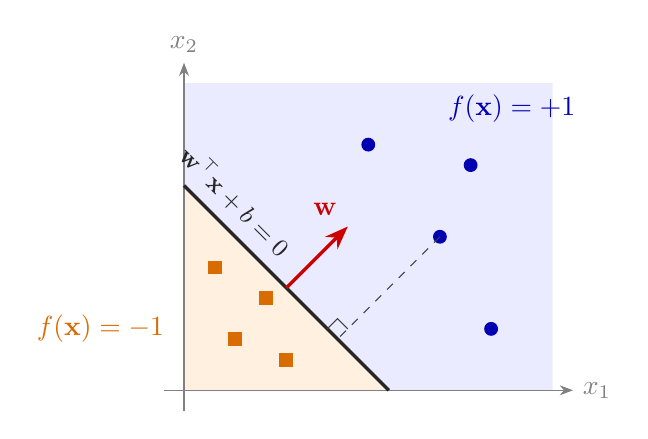
\begin{tikzpicture}[x=1.3cm, y=1.3cm, >=Stealth]
        \fill[blue!8] (2,0) -- (3.6,0) -- (3.6,3) -- (0,3) -- (0,2) -- cycle;
        \fill[orange!12] (0,0) -- (2,0) -- (0,2) -- cycle;
        \draw[->, gray] (-0.2,0) -- (3.8,0) node[right] {$x_1$};
        \draw[->, gray] (0,-0.2) -- (0,3.2) node[above] {$x_2$};
        \draw[very thick, gray!30!black] (0,2) -- (2,0);
        \node[gray!30!black, rotate=-45] at (0.5,1.85) {\small $\mathbf{w}^\top \mathbf{x} + b = 0$};
        \draw[->, very thick, red!80!black] (1,1) -- (1.6,1.6) node[above left] {$\mathbf{w}$};
        \foreach \p in {(2.5,1.5), (3,0.6), (1.8,2.4), (2.8,2.2)} {
            \fill[blue!70!black] \p circle (2.5pt);
        }
        \foreach \p in {(0.5,0.5), (1,0.3), (0.3,1.2), (0.8,0.9)} {
            \fill[orange!85!black] \p ++(-2.5pt,-2.5pt) rectangle ++(5pt,5pt);
        }
        \draw[dashed, gray!50!black] (2.5,1.5) -- (1.5,0.5);
        \draw[gray!50!black] (1.6,0.6) -- (1.5,0.7) -- (1.4,0.6);
        \node[blue!70!black] at (3.2,2.75) {$f(\mathbf{x}) = +1$};
        \node[orange!85!black, left] at (-0.1,0.6) {$f(\mathbf{x}) = -1$};
    \end{tikzpicture}
    \caption[A linear classifier]{A linear classifier in $\mathbb{R}^2$ with $\mathbf{w} = (1, 1)$ and $b = -2$. The decision boundary is the line $x_1 + x_2 = 2$ with normal vector $\mathbf{w}$. Points on the side into which $\mathbf{w}$ points (blue disks) are classified as $+1$, the others (orange squares) as $-1$. The dashed segment shows the distance of the point $(2.5, 1.5)$ to the boundary, which is $\sqrt{2}$ (Example~\ref{L2-ex:classifier-distance}).}
    \label{L2-fig:classifier}
\end{figure}

\section{Inner Products of Functions}

Inner products are not limited to $\mathbb{R}^n$. Functions can be added and multiplied by scalars (Lecture~1), and an integral gives a natural inner product on them.

\begin{proposition}\label{L2-prop:function-ip}
    On the vector space $C[a, b]$ of continuous functions $f: [a, b] \to \mathbb{R}$ (Lecture~1),
    \[\ip{f}{g} = \int_a^b f(x) g(x) \, dx\]
    is an inner product.
\end{proposition}

\begin{proof}
    Bilinearity and symmetry follow from the linearity of the integral. For positive definiteness, $\ip{f}{f} = \int_a^b f(x)^2 \, dx \geq 0$. If $f \neq 0$, then $f(x_0) \neq 0$ for some $x_0$, and by continuity, $f(x)^2 \geq \frac{1}{2} f(x_0)^2$ on some interval of positive length around $x_0$; hence $\ip{f}{f} > 0$.
\end{proof}

The continuity assumption matters: a function that is $1$ at a single point and $0$ everywhere else is nonzero, but the integral of its square is $0$.

\begin{example}
    On $C[-\pi, \pi]$, the functions $\sin$ and $\cos$ are orthogonal, since $\sin(x)\cos(x)$ is an odd function and therefore
    \[\ip{\sin}{\cos} = \int_{-\pi}^{\pi} \sin(x) \cos(x) \, dx = 0.\]
    Moreover, $\norm{\sin}^2 = \int_{-\pi}^{\pi} \sin^2(x) \, dx = \pi$. More generally, the functions $1$, $\cos(x)$, $\sin(x)$, $\cos(2x)$, $\sin(2x)$, \ldots{} are pairwise orthogonal on $[-\pi, \pi]$. Writing a function in terms of them is the idea behind Fourier series, which decompose a signal into frequencies.
\end{example}

\begin{example}[Legendre polynomials]\label{L2-ex:legendre}
    Let us apply the Gram--Schmidt process (unnormalized version) to the polynomials $1, x, x^2, x^3$ in $C[-1, 1]$. We need the integrals $\int_{-1}^1 x^k \, dx$, which are $0$ for odd $k$ and $\frac{2}{k + 1}$ for even $k$:
    \begin{align*}
        u_0 &= 1, \\
        u_1 &= x - \frac{\ip{x}{1}}{\ip{1}{1}} \cdot 1 = x, \\
        u_2 &= x^2 - \frac{\ip{x^2}{1}}{\ip{1}{1}} \cdot 1 - \frac{\ip{x^2}{x}}{\ip{x}{x}} \, x = x^2 - \frac{2/3}{2} = x^2 - \frac{1}{3}, \\
        u_3 &= x^3 - \frac{\ip{x^3}{1}}{\ip{1}{1}} - \frac{\ip{x^3}{x}}{\ip{x}{x}} \, x - \frac{\ip{x^3}{u_2}}{\ip{u_2}{u_2}} \, u_2 = x^3 - \frac{2/5}{2/3} \, x = x^3 - \frac{3}{5} x.
    \end{align*}
    These orthogonal polynomials, shown in Figure~\ref{L2-fig:legendre}, are (up to scaling) the Legendre polynomials. They are used, for example, to approximate functions by polynomials (Exercise~\ref{L2-ex2:best-poly}).
\end{example}

\begin{figure}[ht]
    \centering
    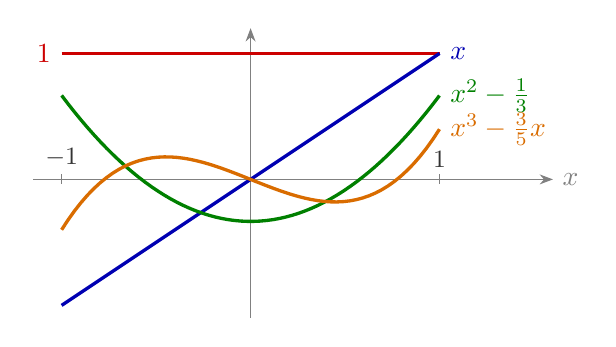
\begin{tikzpicture}[x=2.4cm, y=1.6cm, >=Stealth]
        \draw[->, gray] (-1.15,0) -- (1.6,0) node[right] {$x$};
        \draw[->, gray] (0,-1.1) -- (0,1.2);
        \foreach \t in {-1, 1} {
            \draw[gray] (\t,0.04) -- (\t,-0.04);
            \node[gray!40!black, above] at (\t,0.02) {\small $\t$};
        }
        \draw[very thick, red!80!black] (-1,1) node[left] {$1$} -- (1,1);
        \draw[very thick, blue!70!black] (-1,-1) -- (1,1) node[right] {$x$};
        \draw[very thick, green!50!black, domain=-1:1, samples=60] plot (\x, {\x*\x - 1/3}) node[right] {$x^2 - \frac{1}{3}$};
        \draw[very thick, orange!85!black, domain=-1:1, samples=60] plot (\x, {\x*\x*\x - 0.6*\x}) node[right] {$x^3 - \frac{3}{5}x$};
    \end{tikzpicture}
    \caption[Legendre polynomials]{The orthogonal polynomials of Example~\ref{L2-ex:legendre} on $[-1, 1]$. Any two of them are orthogonal with respect to $\ip{f}{g} = \int_{-1}^1 f(x) g(x) \, dx$.}
    \label{L2-fig:legendre}
\end{figure}

\begin{remark}[Random variables]
    Inner products also appear in probability. For random variables $X$ and $Y$ with mean $0$, the covariance $\mathrm{Cov}(X, Y) = \mathbb{E}[XY]$ behaves like an inner product: it is bilinear, symmetric, and $\mathrm{Cov}(X, X) = \mathrm{Var}(X) \geq 0$. The corresponding norm is the standard deviation, and the correlation coefficient $\frac{\mathrm{Cov}(X, Y)}{\sqrt{\mathrm{Var}(X)\mathrm{Var}(Y)}}$ is the cosine of the angle between $X$ and $Y$. In particular, uncorrelated random variables are orthogonal, and the Cauchy--Schwarz inequality shows that correlations lie between $-1$ and $1$.
\end{remark}

\section{Orthogonal Projections}\label{L2-sec:projections}

Data in machine learning is often high-dimensional, and it is useful to replace each data point by a point of a lower-dimensional subspace while losing as little information as possible. The best way to do this, in a precise sense, is the orthogonal projection. Orthogonal projections are behind linear regression (Section~\ref{L2-sec:least-squares}), principal component analysis (Section~\ref{L2-sec:pca}) and the Gram--Schmidt process.

\begin{definition}[Orthogonal projection]
    Let $U$ be a subspace of a finite-dimensional inner product space $V$. By Theorem~\ref{L2-thm:orth-decomposition}, every $v \in V$ can be written uniquely as $v = u + w$ with $u \in U$ and $w \in U^\perp$. The vector $\pi_U(v) = u$ is called the orthogonal projection of $v$ onto $U$. In other words, $\pi_U(v)$ is the unique vector with
    \[\pi_U(v) \in U \qquad \text{and} \qquad v - \pi_U(v) \in U^\perp.\]
\end{definition}

\begin{proposition}\label{L2-prop:projection-properties}
    Let $U$ be a subspace of a finite-dimensional inner product space $V$.
    \begin{enumerate}
        \item If $e_1, \ldots, e_k$ is an orthonormal basis of $U$, then $\pi_U(v) = \sum_{i=1}^k \ip{v}{e_i} e_i$.
        \item $\pi_U: V \to V$ is a linear transformation with image $U$ and kernel $U^\perp$.
        \item $\pi_U \circ \pi_U = \pi_U$.
    \end{enumerate}
\end{proposition}

\begin{proof}
    (1) This is the formula from the proof of Theorem~\ref{L2-thm:orth-decomposition}. (2) Linearity follows from the formula in part 1. The image is contained in $U$, and $\pi_U(u) = u$ for $u \in U$ (take $w = 0$), so the image is $U$. Moreover, $\pi_U(v) = 0$ if and only if $v = 0 + v$ with $v \in U^\perp$. (3) Since $\pi_U(v) \in U$, we get $\pi_U(\pi_U(v)) = \pi_U(v)$.
\end{proof}

A linear transformation $\pi$ with $\pi \circ \pi = \pi$ is called a projection; for matrices, this is the condition $P^2 = P$ (compare the idempotent matrices in the practice problems of Lecture~1).

\subsection{Projection onto a line}

\begin{proposition}\label{L2-prop:projection-line}
    Let $\mathbf{b} \neq \mathbf{0}$ and $U = \Span\{\mathbf{b}\}$. Then
    \[\pi_U(\mathbf{x}) = \frac{\ip{\mathbf{x}}{\mathbf{b}}}{\ip{\mathbf{b}}{\mathbf{b}}} \, \mathbf{b}.\]
    For the dot product on $\mathbb{R}^n$, this is $\pi_U(\mathbf{x}) = P\mathbf{x}$ with the projection matrix
    \[P = \frac{\mathbf{b} \mathbf{b}^\top}{\mathbf{b}^\top \mathbf{b}},\]
    which is symmetric and satisfies $P^2 = P$.
\end{proposition}

\begin{proof}
    We look for $\pi_U(\mathbf{x}) = \lambda \mathbf{b}$ with $\mathbf{x} - \lambda \mathbf{b} \perp \mathbf{b}$, i.e., $\ip{\mathbf{x}}{\mathbf{b}} - \lambda \ip{\mathbf{b}}{\mathbf{b}} = 0$. This gives $\lambda = \frac{\ip{\mathbf{x}}{\mathbf{b}}}{\ip{\mathbf{b}}{\mathbf{b}}}$. For the dot product, $\lambda \mathbf{b} = \mathbf{b} \lambda = \frac{\mathbf{b} (\mathbf{b}^\top \mathbf{x})}{\mathbf{b}^\top \mathbf{b}} = P\mathbf{x}$. The matrix $\mathbf{b} \mathbf{b}^\top$ is symmetric, and $P^2 = \frac{\mathbf{b} (\mathbf{b}^\top \mathbf{b}) \mathbf{b}^\top}{(\mathbf{b}^\top \mathbf{b})^2} = P$.
\end{proof}

Note that $\mathbf{b}\mathbf{b}^\top$ is an $n \times n$ matrix, while $\mathbf{b}^\top \mathbf{b}$ is a number. The length of the projection is $\norm{\pi_U(\mathbf{x})} = \frac{|\ip{\mathbf{x}}{\mathbf{b}}|}{\norm{\mathbf{b}}} = \norm{\mathbf{x}} \, |\cos\omega|$, where $\omega$ is the angle between $\mathbf{x}$ and $\mathbf{b}$, as in elementary geometry (Figure~\ref{L2-fig:projection-line}).

\begin{figure}[ht]
    \centering
    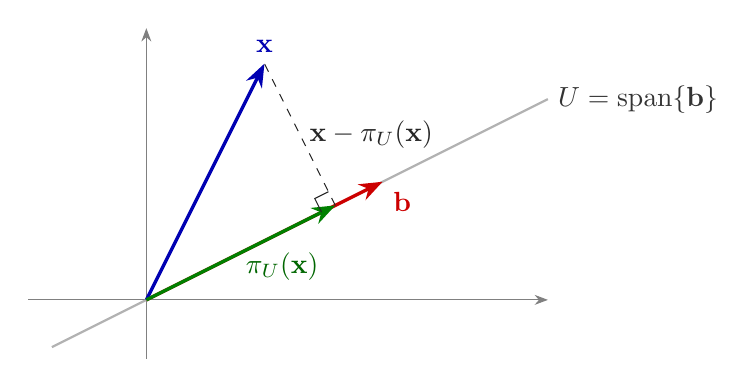
\begin{tikzpicture}[x=1.5cm, y=1.5cm, >=Stealth]
        \draw[->, gray] (-1,0) -- (3.4,0);
        \draw[->, gray] (0,-0.5) -- (0,2.3);
        \draw[thick, gray!60] (-0.8,-0.4) -- (3.4,1.7) node[right, gray!40!black] {$U = \Span\{\mathbf{b}\}$};
        \draw[->, very thick, red!80!black] (0,0) -- (2,1) node[below right] {$\mathbf{b}$};
        \draw[->, very thick, blue!70!black] (0,0) -- (1,2) node[above] {$\mathbf{x}$};
        \draw[->, very thick, green!50!black] (0,0) -- (1.6,0.8);
        \node[green!40!black] at (1.15,0.28) {$\pi_U(\mathbf{x})$};
        \draw[dashed, gray!30!black] (1.6,0.8) -- node[right] {$\mathbf{x} - \pi_U(\mathbf{x})$} (1,2);
        \draw[gray!30!black] (1.484,0.742) -- (1.426,0.858) -- (1.542,0.916);
    \end{tikzpicture}
    \caption[Projection onto a line]{The orthogonal projection of $\mathbf{x} = (1, 2)$ onto the line spanned by $\mathbf{b} = (2, 1)$ is $\pi_U(\mathbf{x}) = \frac{4}{5} \mathbf{b} = (1.6, 0.8)$. The difference $\mathbf{x} - \pi_U(\mathbf{x}) = (-0.6, 1.2)$ is orthogonal to $\mathbf{b}$.}
    \label{L2-fig:projection-line}
\end{figure}

\begin{example}
    Let $\mathbf{b} = (1, 2, 2)^\top$ and $\mathbf{x} = (1, 1, 1)^\top$. Then $\mathbf{b}^\top \mathbf{b} = 9$ and $\mathbf{b}^\top \mathbf{x} = 5$, so
    \[P = \frac{1}{9} \begin{pmatrix} 1 & 2 & 2 \\ 2 & 4 & 4 \\ 2 & 4 & 4 \end{pmatrix}, \qquad \pi_U(\mathbf{x}) = P\mathbf{x} = \frac{5}{9} \begin{pmatrix} 1 \\ 2 \\ 2 \end{pmatrix}.\]
    Indeed, $\mathbf{x} - \pi_U(\mathbf{x}) = \frac{1}{9}(4, -1, -1)^\top$ is orthogonal to $\mathbf{b}$, since $4 - 2 - 2 = 0$.
\end{example}

\subsection{Projection onto a subspace}

Now let $U = \Span\{\mathbf{b}_1, \ldots, \mathbf{b}_m\}$ be an $m$-dimensional subspace of $\mathbb{R}^n$, with the dot product, and let $B$ be the $n \times m$ matrix with columns $\mathbf{b}_1, \ldots, \mathbf{b}_m$, so that $U = \col(B)$.

\begin{theorem}[Normal equations]\label{L2-thm:projection-subspace}
    Let $B$ be an $n \times m$ matrix with linearly independent columns, and $U = \col(B)$. Then for every $\mathbf{x} \in \mathbb{R}^n$,
    \[\pi_U(\mathbf{x}) = B\boldsymbol{\lambda}, \qquad \text{where } \boldsymbol{\lambda} \in \mathbb{R}^m \text{ is the unique solution of } B^\top B \boldsymbol{\lambda} = B^\top \mathbf{x}.\]
    In other words, $\boldsymbol{\lambda} = (B^\top B)^{-1} B^\top \mathbf{x}$, and $\pi_U(\mathbf{x}) = P\mathbf{x}$ with the projection matrix
    \[P = B (B^\top B)^{-1} B^\top.\]
\end{theorem}

\begin{proof}
    Every vector of $U = \col(B)$ has the form $B\boldsymbol{\lambda}$. By Theorem~\ref{L2-thm:fundamental-subspaces}, $U^\perp = \col(B)^\perp = \Null(B^\top)$. So $B\boldsymbol{\lambda} = \pi_U(\mathbf{x})$ if and only if $\mathbf{x} - B\boldsymbol{\lambda} \in \Null(B^\top)$, i.e., $B^\top(\mathbf{x} - B\boldsymbol{\lambda}) = \mathbf{0}$, i.e., $B^\top B \boldsymbol{\lambda} = B^\top \mathbf{x}$. The matrix $B^\top B$ is symmetric positive definite by Example~\ref{L2-ex:BTB}, hence invertible by Proposition~\ref{L2-prop:spd-properties}, so this equation has exactly one solution $\boldsymbol{\lambda} = (B^\top B)^{-1} B^\top \mathbf{x}$.
\end{proof}

The equations $B^\top B \boldsymbol{\lambda} = B^\top \mathbf{x}$ are called the normal equations, since they say that $\mathbf{x} - B\boldsymbol{\lambda}$ is orthogonal (``normal'') to $U$. If the columns of $B$ are orthonormal, then $B^\top B = I_m$, and the formulas simplify to $\boldsymbol{\lambda} = B^\top \mathbf{x}$ and $P = BB^\top$, in agreement with Proposition~\ref{L2-prop:projection-properties}. For $m = 1$, we recover Proposition~\ref{L2-prop:projection-line}.

\begin{example}\label{L2-ex:projection-plane}
    Let $U = \Span\{(1, 1, 1)^\top, (0, 1, 2)^\top\}$ and $\mathbf{x} = (6, 0, 0)^\top$. With $B = \begin{pmatrix} 1 & 0 \\ 1 & 1 \\ 1 & 2 \end{pmatrix}$, we get
    \[B^\top B = \begin{pmatrix} 3 & 3 \\ 3 & 5 \end{pmatrix}, \qquad B^\top \mathbf{x} = \begin{pmatrix} 6 \\ 0 \end{pmatrix}, \qquad \boldsymbol{\lambda} = \begin{pmatrix} 5 \\ -3 \end{pmatrix},\]
    where $\boldsymbol{\lambda}$ solves the normal equations. Hence
    \[\pi_U(\mathbf{x}) = 5 \begin{pmatrix} 1 \\ 1 \\ 1 \end{pmatrix} - 3 \begin{pmatrix} 0 \\ 1 \\ 2 \end{pmatrix} = \begin{pmatrix} 5 \\ 2 \\ -1 \end{pmatrix}, \qquad \mathbf{x} - \pi_U(\mathbf{x}) = \begin{pmatrix} 1 \\ -2 \\ 1 \end{pmatrix},\]
    and indeed $\mathbf{x} - \pi_U(\mathbf{x})$ is orthogonal to both columns of $B$. The projection matrix is
    \[P = B (B^\top B)^{-1} B^\top = \frac{1}{6} \begin{pmatrix} 5 & 2 & -1 \\ 2 & 2 & 2 \\ -1 & 2 & 5 \end{pmatrix}.\]
\end{example}

\begin{proposition}\label{L2-prop:projection-matrix}
    The projection matrix $P = B(B^\top B)^{-1}B^\top$ is symmetric, and $P^2 = P$.
\end{proposition}

\begin{proof}
    $P^2 = B(B^\top B)^{-1} (B^\top B) (B^\top B)^{-1} B^\top = B (B^\top B)^{-1} B^\top = P$. Since $B^\top B$ is symmetric, so is its inverse (Lecture~1: $(A^{-1})^\top = (A^\top)^{-1}$), and therefore $P^\top = B \big((B^\top B)^{-1}\big)^\top B^\top = P$.
\end{proof}

The most important property of the orthogonal projection is that it gives the closest point.

\begin{theorem}[Best approximation]\label{L2-thm:best-approximation}
    Let $U$ be a subspace of a finite-dimensional inner product space $V$, and let $v \in V$. Then $\pi_U(v)$ is the point of $U$ that is closest to $v$:
    \[\norm{v - \pi_U(v)} < \norm{v - u} \qquad \text{for every } u \in U \text{ with } u \neq \pi_U(v).\]
\end{theorem}

\begin{proof}
    Write $v - u = \big(v - \pi_U(v)\big) + \big(\pi_U(v) - u\big)$. The first summand lies in $U^\perp$, and the second one in $U$, so they are orthogonal. By the theorem of Pythagoras,
    \[\norm{v - u}^2 = \norm{v - \pi_U(v)}^2 + \norm{\pi_U(v) - u}^2 > \norm{v - \pi_U(v)}^2,\]
    since $\pi_U(v) - u \neq 0$.
\end{proof}

The number $\norm{v - \pi_U(v)}$ is called the distance from $v$ to $U$. In Example~\ref{L2-ex:projection-plane}, the distance from $\mathbf{x}$ to the plane $U$ is $\norm{(1, -2, 1)^\top} = \sqrt{6}$.

\begin{remark}
    The Gram--Schmidt process (Theorem~\ref{L2-thm:gram-schmidt}) can now be described in one line: $u_j = v_j - \pi_{U_{j-1}}(v_j)$, where $U_{j-1} = \Span\{v_1, \ldots, v_{j-1}\}$. That is, we subtract from $v_j$ its projection onto the span of the previous vectors.
\end{remark}

\subsection{Least squares and linear regression}\label{L2-sec:least-squares}

Suppose we are given data points $(x_1, y_1), \ldots, (x_N, y_N)$ with $x_i, y_i \in \mathbb{R}$, and we want to find the line $y = w_0 + w_1 x$ that fits the data best. In general, no line passes through all points, so we look for the line that minimizes the sum of squared errors
\[\sum_{i=1}^N \big(y_i - (w_0 + w_1 x_i)\big)^2 = \norm{\mathbf{y} - A\mathbf{w}}^2, \qquad \text{where} \quad A = \begin{pmatrix} 1 & x_1 \\ \vdots & \vdots \\ 1 & x_N \end{pmatrix}, \quad \mathbf{y} = \begin{pmatrix} y_1 \\ \vdots \\ y_N \end{pmatrix}, \quad \mathbf{w} = \begin{pmatrix} w_0 \\ w_1 \end{pmatrix}.\]
The matrix $A$ is called the design matrix. This is a special case of the following problem.

\begin{theorem}[Least squares]\label{L2-thm:least-squares}
    Let $A$ be an $N \times n$ matrix with linearly independent columns, and let $\mathbf{y} \in \mathbb{R}^N$. Then there is exactly one $\mathbf{w}^* \in \mathbb{R}^n$ that minimizes $\norm{\mathbf{y} - A\mathbf{w}}$, namely the solution of the normal equations
    \[A^\top A \, \mathbf{w}^* = A^\top \mathbf{y}, \qquad \text{i.e.,} \qquad \mathbf{w}^* = (A^\top A)^{-1} A^\top \mathbf{y}.\]
    Moreover, $A\mathbf{w}^* = \pi_{\col(A)}(\mathbf{y})$.
\end{theorem}

\begin{proof}
    As $\mathbf{w}$ ranges over $\mathbb{R}^n$, the vector $A\mathbf{w}$ ranges over $\col(A)$. By Theorem~\ref{L2-thm:best-approximation}, $\norm{\mathbf{y} - A\mathbf{w}}$ is minimal exactly when $A\mathbf{w} = \pi_{\col(A)}(\mathbf{y})$, and by Theorem~\ref{L2-thm:projection-subspace} (with $B = A$ and $\boldsymbol{\lambda} = \mathbf{w}$), this happens exactly for $\mathbf{w} = (A^\top A)^{-1} A^\top \mathbf{y}$.
\end{proof}

\begin{example}\label{L2-ex:regression}
    Let us fit a line to the data points $(-1, 0)$, $(0, 1)$ and $(1, 3)$. The design matrix and the normal equations are
    \[A = \begin{pmatrix} 1 & -1 \\ 1 & 0 \\ 1 & 1 \end{pmatrix}, \quad \mathbf{y} = \begin{pmatrix} 0 \\ 1 \\ 3 \end{pmatrix}, \qquad A^\top A = \begin{pmatrix} 3 & 0 \\ 0 & 2 \end{pmatrix}, \quad A^\top \mathbf{y} = \begin{pmatrix} 4 \\ 3 \end{pmatrix},\]
    so $\mathbf{w}^* = \big(\frac{4}{3}, \frac{3}{2}\big)^\top$, and the best line is $y =\frac{4}{3} + \frac{3}{2} x$ (Figure~\ref{L2-fig:regression}). The fitted values are $A\mathbf{w}^* = \big(-\frac{1}{6}, \frac{4}{3}, \frac{17}{6}\big)^\top$, the residuals are $\mathbf{y} - A\mathbf{w}^* = \big(\frac{1}{6}, -\frac{1}{3}, \frac{1}{6}\big)^\top$, and the minimal sum of squared errors is $\frac{1}{36} + \frac{1}{9} + \frac{1}{36} = \frac{1}{6}$. As predicted by the theory, the residual vector is orthogonal to both columns of $A$: its entries sum to $0$, and $-\frac{1}{6} + 0 + \frac{1}{6} = 0$.
\end{example}

\begin{figure}[ht]
    \centering
    \begin{tikzpicture}[x=1.5cm, y=1.5cm, >=Stealth]
        \draw[->, gray] (-1.8,0) -- (1.9,0) node[right] {$x$};
        \draw[->, gray] (0,-1) -- (0,3.9) node[above] {$y$};
        \draw[gray] (-1,0.06) -- (-1,-0.06);
        \node[gray!40!black, above left] at (-1,0) {\small $-1$};
        \draw[gray] (1,0.06) -- (1,-0.06) node[below] {\small $1$};
        \foreach \t in {1, 2, 3} {
            \draw[gray] (0.06,\t) -- (-0.06,\t) node[left] {\small $\t$};
        }
        \draw[very thick, blue!70!black, domain=-1.4:1.6] plot (\x, {4/3 + 1.5*\x}) node[right] {$y = \frac{4}{3} + \frac{3}{2}x$};
        \draw[ultra thick, red!80!black] (-1,0) -- (-1,-1/6);
        \draw[ultra thick, red!80!black] (0,1) -- (0,4/3);
        \draw[ultra thick, red!80!black] (1,3) -- (1,17/6);
        \foreach \p in {(-1,0), (0,1), (1,3)} {
            \fill[orange!85!black] \p circle (2pt);
        }
    \end{tikzpicture}
    \caption[Least squares regression]{The least squares line for the data points $(-1, 0)$, $(0, 1)$, $(1, 3)$ (Example~\ref{L2-ex:regression}). The red segments are the residuals; the line minimizes the sum of their squared lengths.}
    \label{L2-fig:regression}
\end{figure}

\begin{remark}[Linear regression in machine learning]
    The same method works for any number of features: each row of the design matrix $A$ contains the features of one data point (and a $1$ for the intercept $w_0$), and the least squares solution gives the weights of the linear model. Using the columns $1, x, x^2, \ldots, x^d$, we can also fit polynomials of degree $d$ (polynomial regression). In practice, the normal equations are not solved by computing $(A^\top A)^{-1}$, but with a QR decomposition or with \py{np.linalg.lstsq}, which are more accurate (compare Lecture~1).
\end{remark}

\subsection{Projections onto affine subspaces and distances to hyperplanes}\label{L2-sec:affine}

Let $L = \mathbf{x}_0 + U$ be an affine subspace, i.e., a subspace $U$ shifted by a vector $\mathbf{x}_0$. To project onto $L$, we shift everything by $-\mathbf{x}_0$, project onto $U$, and shift back:
\[\pi_L(\mathbf{x}) = \mathbf{x}_0 + \pi_U(\mathbf{x} - \mathbf{x}_0).\]
Then $\mathbf{x} - \pi_L(\mathbf{x}) = (\mathbf{x} - \mathbf{x}_0) - \pi_U(\mathbf{x} - \mathbf{x}_0)$ lies in $U^\perp$, and by Theorem~\ref{L2-thm:best-approximation}, $\pi_L(\mathbf{x})$ is the point of $L$ closest to $\mathbf{x}$.

\begin{theorem}[Distance to a hyperplane]\label{L2-thm:distance-hyperplane}
    Let $H = \{\mathbf{z} \in \mathbb{R}^n : \mathbf{w}^\top \mathbf{z} = c\}$ be a hyperplane, where $\mathbf{w} \neq \mathbf{0}$. For every $\mathbf{x} \in \mathbb{R}^n$, the point of $H$ closest to $\mathbf{x}$ is
    \[\pi_H(\mathbf{x}) = \mathbf{x} - \frac{\mathbf{w}^\top \mathbf{x} - c}{\norm{\mathbf{w}}^2}\, \mathbf{w}, \qquad \text{and the distance from } \mathbf{x} \text{ to } H \text{ is} \qquad \frac{|\mathbf{w}^\top \mathbf{x} - c|}{\norm{\mathbf{w}}}.\]
\end{theorem}

\begin{proof}
    Let $\mathbf{x}_0 \in H$, so that $H = \mathbf{x}_0 + W$ with $W = \Span\{\mathbf{w}\}^\perp$, and $W^\perp = \Span\{\mathbf{w}\}$ by Theorem~\ref{L2-thm:orth-decomposition}(3). Since $\mathbf{v} = \pi_W(\mathbf{v}) + \pi_{W^\perp}(\mathbf{v})$ for every $\mathbf{v}$, we get
    \[\mathbf{x} - \pi_H(\mathbf{x}) = (\mathbf{x} - \mathbf{x}_0) - \pi_W(\mathbf{x} - \mathbf{x}_0) = \pi_{\Span\{\mathbf{w}\}}(\mathbf{x} - \mathbf{x}_0) = \frac{\mathbf{w}^\top (\mathbf{x} - \mathbf{x}_0)}{\mathbf{w}^\top \mathbf{w}}\, \mathbf{w} = \frac{\mathbf{w}^\top \mathbf{x} - c}{\norm{\mathbf{w}}^2}\, \mathbf{w},\]
    using Proposition~\ref{L2-prop:projection-line} and $\mathbf{w}^\top \mathbf{x}_0 = c$. Taking the norm gives the distance.
\end{proof}

The number $\frac{\mathbf{w}^\top \mathbf{x} - c}{\norm{\mathbf{w}}}$, without the absolute value, is called the signed distance: it is positive on the side of $H$ into which $\mathbf{w}$ points, and negative on the other side.

\begin{example}
    The distance from the point $\mathbf{x} = (1, 2, 3)^\top$ to the plane $H$ given by $x + 2y + 2z = 2$ is
    \[\frac{|1 + 4 + 6 - 2|}{\sqrt{1 + 4 + 4}} = \frac{9}{3} = 3,\]
    and the closest point of $H$ is $\pi_H(\mathbf{x}) = (1, 2, 3)^\top - \frac{9}{9}(1, 2, 2)^\top = (0, 0, 1)^\top$.
\end{example}

\begin{example}\label{L2-ex:classifier-distance}
    For the linear classifier of Figure~\ref{L2-fig:classifier}, with $\mathbf{w} = (1, 1)^\top$ and $b = -2$, the decision boundary is the hyperplane $\mathbf{w}^\top \mathbf{x} = 2$. The signed distance of the point $\mathbf{x} = (2.5, 1.5)^\top$ to it is $\frac{\mathbf{w}^\top \mathbf{x} + b}{\norm{\mathbf{w}}} = \frac{4 - 2}{\sqrt{2}} = \sqrt{2}$, and the closest point on the boundary is $(2.5, 1.5)^\top - \frac{2}{2}(1, 1)^\top = (1.5, 0.5)^\top$.
\end{example}

\begin{remark}[Margins]
    For a linear classifier, the distance of a data point to the decision boundary is a measure of confidence: points far from the boundary are classified with a large margin. Support vector machines choose the hyperplane that maximizes the smallest distance from the training points to the boundary, which by Theorem~\ref{L2-thm:distance-hyperplane} means maximizing $\min_i \frac{|\mathbf{w}^\top \mathbf{x}_i + b|}{\norm{\mathbf{w}}}$.
\end{remark}

\section{Rotations}\label{L2-sec:rotations}

\begin{definition}[Rotation]
    A rotation of $\mathbb{R}^n$ is an orthogonal $n \times n$ matrix $R$ with $\det(R) = 1$. The set of rotations is denoted by $\mathrm{SO}(n)$, the special orthogonal group.
\end{definition}

By Theorem~\ref{L2-thm:orthogonal}, rotations preserve lengths, distances and angles, and the condition $\det(R) = 1$ means that they preserve the orientation (Lecture~1). Orthogonal matrices with determinant $-1$, such as reflections, reverse the orientation. Since products and inverses of orthogonal matrices are orthogonal, and $\det(R_1 R_2) = \det(R_1)\det(R_2)$, products and inverses of rotations are again rotations; so $\mathrm{SO}(n)$ is a matrix group. The inverse of a rotation $R$ is simply $R^\top$.

\subsection{Rotations in the plane}

In Lecture~1, we met the rotation matrices
\[R_\theta = \begin{pmatrix} \cos\theta & -\sin\theta \\ \sin\theta & \cos\theta \end{pmatrix},\]
which rotate the plane counterclockwise by the angle $\theta$. Every rotation $R$ of $\mathbb{R}^2$ is of this form: its first column $(a, b)^\top$ is a unit vector, so $(a, b) = (\cos\theta, \sin\theta)$ for some angle $\theta$; its second column is a unit vector orthogonal to the first, so it is $\pm(-\sin\theta, \cos\theta)^\top$; and $\det(R) = 1$ forces the sign $+$. Since $R_\alpha R_\beta = R_{\alpha + \beta} = R_\beta R_\alpha$, rotations of the plane commute with each other.

\subsection{Rotations in three dimensions}

The rotations of $\mathbb{R}^3$ by the angle $\theta$ about the three coordinate axes are
\[R_1(\theta) = \begin{pmatrix} 1 & 0 & 0 \\ 0 & \cos\theta & -\sin\theta \\ 0 & \sin\theta & \cos\theta \end{pmatrix}, \quad R_2(\theta) = \begin{pmatrix} \cos\theta & 0 & \sin\theta \\ 0 & 1 & 0 \\ -\sin\theta & 0 & \cos\theta \end{pmatrix}, \quad R_3(\theta) = \begin{pmatrix} \cos\theta & -\sin\theta & 0 \\ \sin\theta & \cos\theta & 0 \\ 0 & 0 & 1 \end{pmatrix}.\]
For example, $R_3(\theta)$ fixes the $x_3$-axis and rotates the $x_1 x_2$-plane by $\theta$. Each of them is orthogonal with determinant $1$. Every rotation of $\mathbb{R}^3$ is a product of such rotations, and it is a rotation about a line through the origin, its axis.

\begin{proposition}[Rotations of $\mathbb{R}^3$]\label{L2-prop:rotations-3d}
    Let $R \in \mathrm{SO}(3)$.
    \begin{enumerate}
        \item (Euler angles.) There are angles $\alpha$, $\beta$ and $\gamma$ with $R = R_3(\alpha)R_1(\beta)R_3(\gamma)$.
        \item (Axis.) There are an orthogonal matrix $Q$ with $\det(Q) = 1$ and an angle $\theta$ with $R = QR_3(\theta)Q^\top$. So $R$ fixes the line spanned by the third column $\mathbf{q}_3$ of $Q$, and it rotates the plane orthogonal to $\mathbf{q}_3$ by the angle $\theta$.
    \end{enumerate}
\end{proposition}

\begin{proof}
    We first show that a rotation $S$ with $S\mathbf{e}_3 = \mathbf{e}_3$ is of the form $R_3(\theta)$. Since $S^\top = S^{-1}$, also $S^\top \mathbf{e}_3 = \mathbf{e}_3$, so the third column and the third row of $S$ are $\mathbf{e}_3$ and $\mathbf{e}_3^\top$:
    \[S = \begin{pmatrix} S' & 0 \\ 0 & 1 \end{pmatrix}\]
    with a $2 \times 2$ matrix $S'$. The columns of $S'$ are orthonormal, since those of $S$ are, and $\det(S') = \det(S) = 1$ (expand along the last row). So $S'$ is a rotation of the plane, $S' = R_\theta$, and $S = R_3(\theta)$.

    (1) The vector $\mathbf{w} = R\mathbf{e}_3$ is a unit vector. Choose $\beta \in [0, \pi]$ with $\cos\beta = w_3$. Then $w_1^2 + w_2^2 = 1 - w_3^2 = \sin^2\beta$, so we can choose $\alpha$ with $(w_1, w_2) = (\sin\alpha\sin\beta, -\cos\alpha\sin\beta)$ (any $\alpha$ if $\sin\beta = 0$). A direct computation gives
    \[R_3(\alpha)R_1(\beta)\mathbf{e}_3 = R_3(\alpha)(0, -\sin\beta, \cos\beta)^\top = (\sin\alpha\sin\beta, -\cos\alpha\sin\beta, \cos\beta)^\top = \mathbf{w}.\]
    Hence $S = \big(R_3(\alpha)R_1(\beta)\big)^{-1}R$ is a rotation with $S\mathbf{e}_3 = \mathbf{e}_3$, so $S = R_3(\gamma)$ for some $\gamma$, and $R = R_3(\alpha)R_1(\beta)R_3(\gamma)$.

    (2) Since $\det(R) = 1$ and $R^\top R = I_3$,
    \[\det(R - I_3) = \det\big(R(I_3 - R^\top)\big) = \det(R)\det\big((I_3 - R)^\top\big) = \det(I_3 - R) = (-1)^3\det(R - I_3).\]
    So $\det(R - I_3) = 0$, and $1$ is an eigenvalue of $R$ (Lecture~1). Let $\mathbf{q}_3$ be a unit vector with $R\mathbf{q}_3 = \mathbf{q}_3$, and let $\mathbf{q}_1, \mathbf{q}_2$ be an orthonormal basis of $\Span\{\mathbf{q}_3\}^\perp$ (Theorem~\ref{L2-thm:orth-decomposition} and Corollary~\ref{L2-cor:onb-exists}). The matrix $Q$ with the columns $\mathbf{q}_1, \mathbf{q}_2, \mathbf{q}_3$ is orthogonal; if $\det(Q) = -1$, we replace $\mathbf{q}_1$ by $-\mathbf{q}_1$. Then $S = Q^\top RQ$ is a rotation with $S\mathbf{e}_3 = Q^\top R\mathbf{q}_3 = Q^\top \mathbf{q}_3 = \mathbf{e}_3$, so $S = R_3(\theta)$, and $R = QR_3(\theta)Q^\top$. The rotation $R_3(\theta)$ fixes $\mathbf{e}_3$ and rotates the plane spanned by $\mathbf{e}_1$ and $\mathbf{e}_2$, and $Q$ maps $\mathbf{e}_1, \mathbf{e}_2, \mathbf{e}_3$ to $\mathbf{q}_1, \mathbf{q}_2, \mathbf{q}_3$.
\end{proof}

In particular, a rotation of $\mathbb{R}^3$ is determined by its axis and its angle. The Euler angles are used, for example, to describe the orientation of a camera or of a robot arm.

\begin{example}
    Unlike in the plane, rotations of $\mathbb{R}^3$ do not commute in general. For $\theta = \frac{\pi}{2}$,
    \[R_1\big(\tfrac{\pi}{2}\big) R_3\big(\tfrac{\pi}{2}\big) = \begin{pmatrix} 0 & -1 & 0 \\ 0 & 0 & -1 \\ 1 & 0 & 0 \end{pmatrix} \neq \begin{pmatrix} 0 & 0 & 1 \\ 1 & 0 & 0 \\ 0 & 1 & 0 \end{pmatrix} = R_3\big(\tfrac{\pi}{2}\big) R_1\big(\tfrac{\pi}{2}\big).\]
    For instance, the first product maps $\mathbf{e}_1$ to $\mathbf{e}_3$, while the second maps $\mathbf{e}_1$ to $\mathbf{e}_2$. You can check this with a book: rotate it first about one axis and then about another, and compare with the opposite order.
\end{example}

\subsection{\texorpdfstring{Rotations in $n$ dimensions}{Rotations in n dimensions}}

\begin{definition}[Givens rotation]
    For $1 \leq i < j \leq n$ and an angle $\theta$, the Givens rotation $G_{ij}(\theta)$ is the $n \times n$ matrix that agrees with the identity matrix, except for the four entries
    \[G_{ii} = \cos\theta, \qquad G_{ij} = -\sin\theta, \qquad G_{ji} = \sin\theta, \qquad G_{jj} = \cos\theta.\]
\end{definition}

The Givens rotation $G_{ij}(\theta)$ rotates the plane spanned by $\mathbf{e}_i$ and $\mathbf{e}_j$ by the angle $\theta$, and fixes all other standard basis vectors. Its columns are orthonormal, and its determinant is $\cos^2\theta + \sin^2\theta = 1$ (expand along the other rows), so it is a rotation. Givens rotations are used in numerical linear algebra: a well-chosen Givens rotation makes a chosen entry of a matrix zero, and a sequence of them computes a QR decomposition.

\begin{remark}[Rotations in machine learning]
    Since rotations preserve dot products and distances, any method that only depends on distances or dot products between data points, such as $k$-nearest neighbors with the Euclidean distance, gives the same results after the data is rotated. In contrast, methods such as decision trees, which look at individual coordinates, may change. Rotated copies of images are also used for data augmentation, to make image classifiers robust to rotations.
\end{remark}

\section{The Spectral Theorem}\label{L2-sec:spectral}

In Lecture~1, we saw that a matrix is diagonalizable if it has a basis of eigenvectors, and that some matrices, such as the shear or a rotation, are not diagonalizable. Symmetric matrices are much better behaved: they always have an orthonormal basis of eigenvectors. Symmetric matrices are everywhere in machine learning: covariance matrices, Gram and kernel matrices, and the matrices $A^\top A$ of least squares problems are all symmetric.

To state the theorem, we use complex eigenvalues (Lecture~1). For a vector $\mathbf{v} \in \mathbb{C}^n$, we write $\bar{\mathbf{v}}$ for the vector of complex conjugates of its entries. Then $\bar{\mathbf{v}}^\top \mathbf{v} = \sum_i \bar{\mathbf{v}}_i v_i = \sum_i |v_i|^2 > 0$ for $\mathbf{v} \neq \mathbf{0}$. A complex number $\lambda$ is a root of $p_A$ if and only if $A\mathbf{v} = \lambda \mathbf{v}$ for some nonzero $\mathbf{v} \in \mathbb{C}^n$, by the same argument as for real eigenvalues.

\begin{theorem}[Spectral theorem]\label{L2-thm:spectral}
    Let $A$ be a symmetric real $n \times n$ matrix. Then:
    \begin{enumerate}
        \item all complex eigenvalues of $A$ are real;
        \item eigenvectors of $A$ for distinct eigenvalues are orthogonal;
        \item there is an orthonormal basis $\mathbf{q}_1, \ldots, \mathbf{q}_n$ of $\mathbb{R}^n$ consisting of eigenvectors of $A$. Equivalently,
        \[A = Q \Lambda Q^\top,\]
        where $Q$ is the orthogonal matrix with columns $\mathbf{q}_1, \ldots, \mathbf{q}_n$, and $\Lambda = \diag(\lambda_1, \ldots, \lambda_n)$ contains the corresponding eigenvalues.
    \end{enumerate}
\end{theorem}

\begin{proof}
    (1) Let $A\mathbf{v} = \lambda \mathbf{v}$ with $\lambda \in \mathbb{C}$ and $\mathbf{v} \in \mathbb{C}^n$, $\mathbf{v} \neq \mathbf{0}$. The number $z = \bar{\mathbf{v}}^\top A \mathbf{v}$ is real: since $A$ is real and symmetric, its complex conjugate is $\bar{z} = \mathbf{v}^\top A \bar{\mathbf{v}} = (\mathbf{v}^\top A \bar{\mathbf{v}})^\top = \bar{\mathbf{v}}^\top A^\top \mathbf{v} = z$. Since $z = \bar{\mathbf{v}}^\top (\lambda \mathbf{v}) = \lambda\, \bar{\mathbf{v}}^\top \mathbf{v}$, we get $\lambda = z / (\bar{\mathbf{v}}^\top \mathbf{v}) \in \mathbb{R}$.

    (2) Let $A\mathbf{v} = \lambda \mathbf{v}$ and $A\mathbf{w} = \mu \mathbf{w}$ with $\lambda \neq \mu$. Then
    \[\lambda\, \mathbf{v}^\top \mathbf{w} = (A\mathbf{v})^\top \mathbf{w} = \mathbf{v}^\top A^\top \mathbf{w} = \mathbf{v}^\top A \mathbf{w} = \mu\, \mathbf{v}^\top \mathbf{w},\]
    so $(\lambda - \mu) \mathbf{v}^\top \mathbf{w} = 0$, and hence $\mathbf{v}^\top \mathbf{w} = 0$.

    (3) We use induction on $n$; the case $n = 1$ is clear. By part 1 and the fundamental theorem of algebra, $p_A$ has a real root $\lambda_1$. Let $\mathbf{q}_1$ be a unit eigenvector for $\lambda_1$ (it can be chosen real, since $A - \lambda_1 I_n$ is a real matrix with a nonzero null space). Let $W = \Span\{\mathbf{q}_1\}^\perp$, and let $\mathbf{w}_2, \ldots, \mathbf{w}_n$ be an orthonormal basis of $W$ (Theorem~\ref{L2-thm:orth-decomposition} and Corollary~\ref{L2-cor:onb-exists}). The subspace $W$ is mapped into itself by $A$: if $\mathbf{x} \in W$, then $\mathbf{q}_1^\top (A\mathbf{x}) = (A\mathbf{q}_1)^\top \mathbf{x} = \lambda_1 \mathbf{q}_1^\top \mathbf{x} = 0$.

    Let $M$ be the $n \times (n-1)$ matrix with columns $\mathbf{w}_2, \ldots, \mathbf{w}_n$, so that $M^\top M = I_{n-1}$, and let $B = M^\top A M$, which is a symmetric $(n-1) \times (n-1)$ matrix. Since $A\mathbf{w}_i \in W$, Proposition~\ref{L2-prop:onb-coordinates} gives $A\mathbf{w}_i = \sum_k (\mathbf{w}_k^\top A \mathbf{w}_i) \mathbf{w}_k$, i.e., $AM = MB$. By induction, $B$ has an orthonormal basis of eigenvectors $\mathbf{y}_2, \ldots, \mathbf{y}_n \in \mathbb{R}^{n-1}$, with $B\mathbf{y}_j = \lambda_j \mathbf{y}_j$. Then the vectors $\mathbf{q}_j = M \mathbf{y}_j$ ($j = 2, \ldots, n$) are orthonormal, since $\mathbf{q}_i^\top \mathbf{q}_j = \mathbf{y}_i^\top M^\top M \mathbf{y}_j = \mathbf{y}_i^\top \mathbf{y}_j$; they lie in $W$, so they are orthogonal to $\mathbf{q}_1$; and they are eigenvectors, since $A\mathbf{q}_j = AM\mathbf{y}_j = MB\mathbf{y}_j = \lambda_j \mathbf{q}_j$. So $\mathbf{q}_1, \ldots, \mathbf{q}_n$ is an orthonormal basis of eigenvectors.

    Finally, by Theorem~\ref{L2-thm:orthogonal}, $Q$ is orthogonal, so $Q^{-1} = Q^\top$, and by the diagonalization theorem of Lecture~1, $A = Q\Lambda Q^{-1} = Q\Lambda Q^\top$.
\end{proof}

The factorization $A = Q\Lambda Q^\top$ is called the eigendecomposition, or spectral decomposition, of $A$. Multiplying out, it says that
\[A = \lambda_1 \mathbf{q}_1 \mathbf{q}_1^\top + \lambda_2 \mathbf{q}_2 \mathbf{q}_2^\top + \cdots + \lambda_n \mathbf{q}_n \mathbf{q}_n^\top,\]
where each $\mathbf{q}_i \mathbf{q}_i^\top$ is the matrix of the orthogonal projection onto the line $\Span\{\mathbf{q}_i\}$ (Proposition~\ref{L2-prop:projection-line}). So a symmetric matrix projects a vector onto $n$ orthogonal directions, scales the projections by the eigenvalues, and adds them up.

\begin{example}\label{L2-ex:spectral}
    Let $A = \begin{pmatrix} 2 & 1 & 1 \\ 1 & 2 & 1 \\ 1 & 1 & 2 \end{pmatrix} = J + 2I_3$, where $J = \begin{pmatrix} 0 & 1 & 1 \\ 1 & 0 & 1 \\ 1 & 1 & 0 \end{pmatrix}$ is the matrix from the section on eigenvalues in Lecture~1. By the computations there, the eigenvalues of $A$ are $2 + 2 = 4$, with eigenspace $\Span\{(1, 1, 1)^\top\}$, and $-1 + 2 = 1$, with eigenspace the plane $x + y + z = 0$. As predicted by the spectral theorem, the two eigenspaces are orthogonal. To get an orthonormal basis of the plane, we apply the Gram--Schmidt process to its basis $(1, -1, 0)^\top$, $(1, 0, -1)^\top$, which gives $\frac{1}{\sqrt{2}}(1, -1, 0)^\top$ and $\frac{1}{\sqrt{6}}(1, 1, -2)^\top$. Hence $A = Q\Lambda Q^\top$ with
    \[Q = \begin{pmatrix} \frac{1}{\sqrt{3}} & \frac{1}{\sqrt{2}} & \frac{1}{\sqrt{6}} \\ \frac{1}{\sqrt{3}} & -\frac{1}{\sqrt{2}} & \frac{1}{\sqrt{6}} \\ \frac{1}{\sqrt{3}} & 0 & -\frac{2}{\sqrt{6}} \end{pmatrix}, \qquad \Lambda = \diag(4, 1, 1).\]
\end{example}

\begin{corollary}\label{L2-cor:spd-eigenvalues}
    A symmetric matrix is positive definite if and only if all its eigenvalues are positive, and positive semidefinite if and only if all its eigenvalues are nonnegative.
\end{corollary}

\begin{proof}
    Write $A = Q\Lambda Q^\top$ and $\mathbf{y} = Q^\top \mathbf{x}$. Then
    \[\mathbf{x}^\top A \mathbf{x} = \mathbf{y}^\top \Lambda \mathbf{y} = \lambda_1 y_1^2 + \cdots + \lambda_n y_n^2.\]
    If all $\lambda_i > 0$, this is positive for $\mathbf{x} \neq \mathbf{0}$ (then $\mathbf{y} \neq \mathbf{0}$, since $Q^\top$ is invertible). Conversely, $\mathbf{q}_i^\top A \mathbf{q}_i = \lambda_i$, so if $A$ is positive definite, all $\lambda_i > 0$. The semidefinite case is the same, with $\geq$ instead of $>$.
\end{proof}

\begin{corollary}[Sylvester's criterion]\label{L2-cor:sylvester}
    Let $A$ be a symmetric $n \times n$ matrix, and let $A_k$ be its upper left $k \times k$ submatrix, with the entries $A_{ij}$ for $i, j \leq k$. Then $A$ is positive definite if and only if $\det(A_k) > 0$ for $k = 1, \ldots, n$.
\end{corollary}

\begin{proof}
    For $\mathbf{x} \in \mathbb{R}^k$, let $\tilde{\mathbf{x}} \in \mathbb{R}^n$ be $\mathbf{x}$ followed by $n - k$ zeros. Then $\mathbf{x}^\top A_k \mathbf{x} = \tilde{\mathbf{x}}^\top A\tilde{\mathbf{x}}$. So if $A$ is positive definite, then so is every $A_k$. By Corollary~\ref{L2-cor:spd-eigenvalues}, the eigenvalues of $A_k$ are positive, and $\det(A_k)$, which is their product (Lecture~1), is positive.

    For the converse, we use induction on $n$; for $n = 1$, $A = (A_{11})$ with $A_{11} > 0$. Let $n \geq 2$, and assume that all $\det(A_k) > 0$. By induction, $A_{n-1}$ is positive definite. The eigenvalues $\lambda_1, \ldots, \lambda_n$ of $A$ have the positive product $\det(A)$, so none of them is $0$, and the number of negative ones is even. Suppose that $A$ is not positive definite. Then at least two eigenvalues are negative, say $\lambda_i, \lambda_j < 0$ with $i \neq j$, with orthonormal eigenvectors $\mathbf{q}_i$ and $\mathbf{q}_j$. The equation $a(\mathbf{q}_i)_n + b(\mathbf{q}_j)_n = 0$ has a solution $(a, b) \neq (0, 0)$, and then $\mathbf{x} = a\mathbf{q}_i + b\mathbf{q}_j$ is nonzero (as $\mathbf{q}_i$ and $\mathbf{q}_j$ are linearly independent), and its last entry is $0$. On the one hand, $\mathbf{x}^\top A\mathbf{x} = \lambda_i a^2 + \lambda_j b^2 < 0$. On the other hand, $\mathbf{x} = \tilde{\mathbf{x}}'$ for some nonzero $\mathbf{x}' \in \mathbb{R}^{n-1}$, so $\mathbf{x}^\top A\mathbf{x} = \mathbf{x}'^\top A_{n-1}\mathbf{x}' > 0$. This is a contradiction.
\end{proof}

For example, the matrix $A = J + 2I_3$ of Example~\ref{L2-ex:spectral} has $\det(A_1) = 2$, $\det(A_2) = 3$ and $\det(A_3) = 4$, so it is positive definite, in agreement with its eigenvalues $4, 1, 1$.

\begin{example}
    The matrix $\begin{pmatrix} 9 & 6 \\ 6 & 5 \end{pmatrix}$ from the subsection on symmetric positive definite matrices has trace $14$ and determinant $9$, so its eigenvalues $7 \pm 2\sqrt{10}$ are both positive, and it is positive definite. The matrix $\begin{pmatrix} 9 & 6 \\ 6 & 3 \end{pmatrix}$ has determinant $-9 < 0$, so its eigenvalues have opposite signs (their product is negative), and it is not positive definite.
\end{example}

\begin{proposition}[Rayleigh quotient]\label{L2-prop:rayleigh}
    Let $A$ be symmetric with eigenvalues $\lambda_1 \geq \lambda_2 \geq \cdots \geq \lambda_n$ and orthonormal eigenvectors $\mathbf{q}_1, \ldots, \mathbf{q}_n$. Then for every $\mathbf{x} \neq \mathbf{0}$,
    \[\lambda_n \leq \frac{\mathbf{x}^\top A \mathbf{x}}{\mathbf{x}^\top \mathbf{x}} \leq \lambda_1,\]
    with equality on the right for $\mathbf{x} = \mathbf{q}_1$, and on the left for $\mathbf{x} = \mathbf{q}_n$.
\end{proposition}

\begin{proof}
    With $\mathbf{y} = Q^\top \mathbf{x}$, we have $\mathbf{x}^\top \mathbf{x} = \mathbf{y}^\top \mathbf{y}$ (Theorem~\ref{L2-thm:orthogonal}) and $\mathbf{x}^\top A \mathbf{x} = \sum_i \lambda_i y_i^2$, which lies between $\lambda_n \sum_i y_i^2$ and $\lambda_1 \sum_i y_i^2$. For $\mathbf{x} = \mathbf{q}_i$, the quotient is $\mathbf{q}_i^\top A \mathbf{q}_i = \lambda_i$.
\end{proof}

So the largest eigenvalue of a symmetric matrix is the maximum of $\mathbf{x}^\top A \mathbf{x}$ over all unit vectors $\mathbf{x}$, and it is attained at an eigenvector. This is the key to principal component analysis. More generally, the sum of the $k$ largest eigenvalues is the maximum of $\sum_j \mathbf{b}_j^\top A\mathbf{b}_j$ over $k$ orthonormal vectors $\mathbf{b}_1, \ldots, \mathbf{b}_k$.

\begin{proposition}[Ky Fan]\label{L2-prop:ky-fan}
    Let $A$ be symmetric with eigenvalues $\lambda_1 \geq \lambda_2 \geq \cdots \geq \lambda_n$ and orthonormal eigenvectors $\mathbf{q}_1, \ldots, \mathbf{q}_n$, and let $1 \leq k \leq n$. For every $n \times k$ matrix $B$ with orthonormal columns $\mathbf{b}_1, \ldots, \mathbf{b}_k$,
    \[\tr(B^\top AB) = \sum_{j=1}^k \mathbf{b}_j^\top A\mathbf{b}_j \leq \lambda_1 + \cdots + \lambda_k,\]
    with equality for $\mathbf{b}_j = \mathbf{q}_j$, $j = 1, \ldots, k$.
\end{proposition}

\begin{proof}
    Writing $\mathbf{b}_j = \sum_i (\mathbf{q}_i^\top \mathbf{b}_j)\mathbf{q}_i$ (Proposition~\ref{L2-prop:onb-coordinates}) gives $\mathbf{b}_j^\top A\mathbf{b}_j = \sum_i \lambda_i (\mathbf{q}_i^\top \mathbf{b}_j)^2$, so
    \[\tr(B^\top AB) = \sum_{i=1}^n \lambda_i c_i, \qquad \text{where } c_i = \sum_{j=1}^k (\mathbf{q}_i^\top \mathbf{b}_j)^2 = \norm{B^\top \mathbf{q}_i}^2.\]
    The numbers $c_i$ satisfy $\sum_i c_i = \sum_j \sum_i (\mathbf{q}_i^\top \mathbf{b}_j)^2 = \sum_j \norm{\mathbf{b}_j}^2 = k$ and $0 \leq c_i \leq 1$: extending $\mathbf{b}_1, \ldots, \mathbf{b}_k$ to an orthonormal basis $\mathbf{b}_1, \ldots, \mathbf{b}_n$ of $\mathbb{R}^n$ gives $c_i \leq \sum_{j=1}^n (\mathbf{b}_j^\top \mathbf{q}_i)^2 = \norm{\mathbf{q}_i}^2 = 1$. Since $\lambda_i \geq \lambda_k$ and $c_i - 1 \leq 0$ for $i \leq k$, and $\lambda_i \leq \lambda_k$ and $c_i \geq 0$ for $i > k$,
    \[\sum_{i=1}^n \lambda_i c_i - \sum_{i=1}^k \lambda_i = \sum_{i \leq k} \lambda_i(c_i - 1) + \sum_{i > k} \lambda_i c_i \leq \lambda_k\sum_{i \leq k}(c_i - 1) + \lambda_k\sum_{i > k} c_i = \lambda_k\Big(\sum_{i=1}^n c_i - k\Big) = 0.\]
    For $\mathbf{b}_j = \mathbf{q}_j$, $\tr(B^\top AB) = \sum_{j \leq k} \mathbf{q}_j^\top A\mathbf{q}_j = \lambda_1 + \cdots + \lambda_k$.
\end{proof}

\begin{remark}[Geometry of symmetric positive definite matrices]
    If $A$ is symmetric positive definite, the set $\{\mathbf{x} : \mathbf{x}^\top A \mathbf{x} = 1\}$ is an ellipse (in $\mathbb{R}^2$) or an ellipsoid (in higher dimensions), whose axes point in the directions of the eigenvectors $\mathbf{q}_i$ and have lengths $\frac{1}{\sqrt{\lambda_i}}$, since in the coordinates $\mathbf{y} = Q^\top \mathbf{x}$ the equation becomes $\lambda_1 y_1^2 + \cdots + \lambda_n y_n^2 = 1$. In machine learning, such ellipsoids describe the shape of Gaussian distributions (with $A$ the inverse covariance matrix) and the shape of the loss surface of least squares problems near a minimum; when the eigenvalues have very different sizes, gradient descent zig-zags and converges slowly.
\end{remark}

\subsection{The graph Laplacian and spectral clustering}\label{L2-sec:laplacian}

Many data sets are graphs: users connected by friendships, web pages by links, molecules by bonds, or data points connected to their nearest neighbors. A weighted graph on the vertices $1, \ldots, n$ is described by a symmetric $n \times n$ matrix $W$ of weights $w_{ij} = w_{ji} \geq 0$, with $w_{ii} = 0$; there is an edge between $i$ and $j$ if $w_{ij} > 0$. For example, $w_{ij} = 1$ for the pairs of friends, or $w_{ij} = e^{-\norm{\mathbf{x}_i - \mathbf{x}_j}^2/(2s^2)}$ for data points $\mathbf{x}_i$ that are close to each other. A symmetric matrix describes the graph, and the spectral theorem describes its shape.

\begin{definition}[Graph Laplacian]\label{L2-def:laplacian}
    The degree of the vertex $i$ is $d_i = \sum_j w_{ij}$. The Laplacian of the graph is the matrix $L = D - W$, where $D = \diag(d_1, \ldots, d_n)$.
\end{definition}

\begin{proposition}\label{L2-prop:laplacian}
    For every $\mathbf{x} \in \mathbb{R}^n$,
    \[\mathbf{x}^\top L\mathbf{x} = \sum_{i < j} w_{ij}(x_i - x_j)^2.\]
    Hence $L$ is symmetric and positive semidefinite, and $L\mathbf{1} = \mathbf{0}$ for the vector $\mathbf{1} = (1, \ldots, 1)^\top$.
\end{proposition}

\begin{proof}
    $\mathbf{x}^\top L\mathbf{x} = \sum_i d_ix_i^2 - \sum_{i, j} w_{ij}x_ix_j = \frac{1}{2}\sum_{i, j} w_{ij}(x_i^2 + x_j^2 - 2x_ix_j) = \frac{1}{2}\sum_{i, j} w_{ij}(x_i - x_j)^2$, using $\sum_i d_ix_i^2 = \sum_{i, j} w_{ij}x_i^2 = \sum_{i, j} w_{ij}x_j^2$; the terms with $i = j$ vanish, and those with $i > j$ repeat those with $i < j$. The rows of $L$ sum to $d_i - \sum_j w_{ij} = 0$.
\end{proof}

So $\mathbf{x}^\top L\mathbf{x}$ is small if $\mathbf{x}$ varies little along the edges with large weights: it measures how smooth a function $\mathbf{x}$ on the vertices is. The vertices $i$ and $j$ are in the same connected component of the graph if there is a path $i = i_0, i_1, \ldots, i_l = j$ with $w_{i_{s-1}i_s} > 0$ for every step.

\begin{theorem}\label{L2-thm:laplacian-components}
    Let $L$ be the Laplacian of a graph with the connected components $C_1, \ldots, C_k$. Then $\Null(L)$ is spanned by the indicator vectors $\mathbf{1}_{C_1}, \ldots, \mathbf{1}_{C_k}$ (with the entries $1$ on $C_l$ and $0$ elsewhere). So the multiplicity of the eigenvalue $0$ is the number of connected components; in particular, the graph is connected if and only if the second smallest eigenvalue $\lambda_2$ of $L$ is positive.
\end{theorem}

\begin{proof}
    Write $L = Q\Lambda Q^\top$ with eigenvalues $\lambda_i \geq 0$ (Corollary~\ref{L2-cor:spd-eigenvalues}), and let $\mathbf{y} = Q^\top \mathbf{x}$. If $\mathbf{x}^\top L\mathbf{x} = \sum_i \lambda_iy_i^2 = 0$, then $y_i = 0$ whenever $\lambda_i > 0$, so $L\mathbf{x} = Q\Lambda \mathbf{y} = \mathbf{0}$; the converse is clear. So $L\mathbf{x} = \mathbf{0}$ if and only if $\mathbf{x}^\top L\mathbf{x} = 0$, i.e., by Proposition~\ref{L2-prop:laplacian}, if and only if $x_i = x_j$ whenever $w_{ij} > 0$. Following paths, this means that $\mathbf{x}$ is constant on each connected component, i.e., $\mathbf{x} = \sum_l c_l\mathbf{1}_{C_l}$. The vectors $\mathbf{1}_{C_l}$ are nonzero and orthogonal, hence linearly independent (Lemma~\ref{L2-lem:orth-indep}), so $\dim\Null(L) = k$, which is the multiplicity of the eigenvalue $0$ in the spectral decomposition.
\end{proof}

\paragraph{Spectral clustering.} Clustering means splitting the vertices into groups with many edges inside the groups and few edges between them. For a set $A$ of vertices and its complement $\bar{A}$, the weight of the edges between them is $\mathrm{cut}(A) = \sum_{i \in A, \, j \in \bar{A}} w_{ij}$. Minimizing the cut alone tends to split off single vertices, so one balances it by the sizes of the parts:
\[\mathrm{RatioCut}(A) = \mathrm{cut}(A)\Big(\frac{1}{|A|} + \frac{1}{|\bar{A}|}\Big).\]
Finding the best $A$ is a hard combinatorial problem, since there are $2^{n-1} - 1$ ways to split the vertices into two nonempty parts. The Laplacian turns it into an eigenvalue problem.

\begin{theorem}\label{L2-thm:ratio-cut}
    Let $0 = \lambda_1 \leq \lambda_2 \leq \cdots \leq \lambda_n$ be the eigenvalues of the Laplacian of a graph. For every set of vertices $A$ with $A \neq \emptyset$ and $\bar{A} \neq \emptyset$, define $\mathbf{f} \in \mathbb{R}^n$ by $f_i = \sqrt{|\bar{A}|/|A|}$ for $i \in A$ and $f_i = -\sqrt{|A|/|\bar{A}|}$ for $i \in \bar{A}$. Then
    \[\mathbf{f}^\top\mathbf{1} = 0, \qquad \norm{\mathbf{f}}^2 = n, \qquad \mathbf{f}^\top L\mathbf{f} = n\,\mathrm{RatioCut}(A), \qquad \text{and hence} \qquad \mathrm{RatioCut}(A) \geq \lambda_2.\]
\end{theorem}

\begin{proof}
    $\mathbf{f}^\top\mathbf{1} = |A|\sqrt{|\bar{A}|/|A|} - |\bar{A}|\sqrt{|A|/|\bar{A}|} = \sqrt{|A||\bar{A}|} - \sqrt{|A||\bar{A}|} = 0$, and $\norm{\mathbf{f}}^2 = |\bar{A}| + |A| = n$. In Proposition~\ref{L2-prop:laplacian}, only the edges between $A$ and $\bar{A}$ contribute, each with
    \[(f_i - f_j)^2 = \frac{|\bar{A}|}{|A|} + \frac{|A|}{|\bar{A}|} + 2 = \frac{(|A| + |\bar{A}|)^2}{|A||\bar{A}|} = n\Big(\frac{1}{|A|} + \frac{1}{|\bar{A}|}\Big),\]
    which gives $\mathbf{f}^\top L\mathbf{f} = n\,\mathrm{RatioCut}(A)$. Let $\mathbf{q}_1 = \frac{1}{\sqrt{n}}\mathbf{1}, \mathbf{q}_2, \ldots, \mathbf{q}_n$ be orthonormal eigenvectors of $L$. Since $\mathbf{f}$ is orthogonal to $\mathbf{q}_1$, it is $\mathbf{f} = \sum_{i \geq 2} c_i\mathbf{q}_i$, and $\mathbf{f}^\top L\mathbf{f} = \sum_{i \geq 2} \lambda_ic_i^2 \geq \lambda_2\norm{\mathbf{f}}^2 = n\lambda_2$.
\end{proof}

The proof also shows that $\lambda_2$ is the minimum of $\frac{\mathbf{x}^\top L\mathbf{x}}{\mathbf{x}^\top \mathbf{x}}$ over all $\mathbf{x} \neq \mathbf{0}$ with $\mathbf{x}^\top\mathbf{1} = 0$, attained at an eigenvector $\mathbf{q}_2$, which is called the Fiedler vector. Minimizing over the special vectors $\mathbf{f}$ of the theorem is hard, but minimizing over all vectors orthogonal to $\mathbf{1}$ is an eigenvalue problem. This suggests spectral clustering: compute the Fiedler vector $\mathbf{q}_2$, and put the vertices with $(\mathbf{q}_2)_i \geq 0$ into one cluster and the others into the second one. For $k$ clusters, one represents each vertex $i$ by the $i$-th row of the $n \times k$ matrix of the eigenvectors $\mathbf{q}_1, \ldots, \mathbf{q}_k$ and clusters these points with $k$-means (Section~\ref{L4-sec:latent}).

\begin{example}\label{L2-ex:two-triangles}
    Take two triangles on the vertices $\{1, 2, 3\}$ and $\{4, 5, 6\}$, joined by the edge between $3$ and $4$, all with weight $1$. One checks that $L\mathbf{x} = \lambda \mathbf{x}$ for $\mathbf{x} = (1, 1, t, -t, -1, -1)^\top$ if $1 - t = \lambda$ (the equation for vertex $1$) and $4t - 2 = \lambda t$ (vertex $3$), i.e., $\lambda^2 - 5\lambda + 2 = 0$. The smaller root $\lambda_2 = \frac{5 - \sqrt{17}}{2} \approx 0.44$ is the second smallest eigenvalue (the others are $0$, $3$, $3$, $3$ and $\frac{5 + \sqrt{17}}{2}$), with $t = \frac{\sqrt{17} - 3}{2} \approx 0.56$. The signs of the Fiedler vector separate the two triangles, and for $A = \{1, 2, 3\}$, $\mathrm{RatioCut}(A) = 1 \cdot (\frac{1}{3} + \frac{1}{3}) = \frac{2}{3} \geq \lambda_2$, as predicted.
\end{example}

\begin{remark}[Graphs in machine learning]
    The quadratic form $\mathbf{x}^\top L\mathbf{x}$ is used as a smoothness penalty in semi-supervised learning: labels known on a few vertices are extended to the whole graph by minimizing $\mathbf{x}^\top L\mathbf{x}$ subject to the known values, so that neighbors get similar labels. Laplacian eigenmaps embed data points by the eigenvectors $\mathbf{q}_2, \mathbf{q}_3, \ldots$, and graph neural networks update the features of each vertex by averaging over its neighbors with matrices such as $D^{-1/2}WD^{-1/2}$, which are closely related to the Laplacian.
\end{remark}

\section{The Singular Value Decomposition}\label{L2-sec:svd}

The eigendecomposition only exists for square matrices, and in general only for diagonalizable ones. The singular value decomposition (SVD) exists for every matrix, square or not. It is one of the most useful factorizations in applied mathematics and machine learning: it describes the geometry of every linear transformation, gives the best low-rank approximations of a matrix, and is the basis of principal component analysis.

\subsection{Existence of the SVD}

\begin{theorem}[Singular value decomposition]\label{L2-thm:svd}
    Let $A$ be a real $m \times n$ matrix. Then there are an orthogonal $m \times m$ matrix $U$, an orthogonal $n \times n$ matrix $V$, and an $m \times n$ matrix $\Sigma$ with
    \[\Sigma_{11} = \sigma_1 \geq \Sigma_{22} = \sigma_2 \geq \cdots \geq \Sigma_{rr} = \sigma_r > 0\]
    and all other entries $0$, such that
    \[A = U \Sigma V^\top.\]
    The number $r$ of nonzero diagonal entries is the rank of $A$. The numbers $\sigma_1, \ldots, \sigma_r$ are called the singular values of $A$; the columns $\mathbf{u}_1, \ldots, \mathbf{u}_m$ of $U$ and $\mathbf{v}_1, \ldots, \mathbf{v}_n$ of $V$ are called the left and right singular vectors of $A$.
\end{theorem}

\begin{proof}
    The $n \times n$ matrix $A^\top A$ is symmetric, and positive semidefinite, since $\mathbf{x}^\top A^\top A \mathbf{x} = \norm{A\mathbf{x}}^2 \geq 0$. By the spectral theorem and Corollary~\ref{L2-cor:spd-eigenvalues}, there is an orthonormal basis $\mathbf{v}_1, \ldots, \mathbf{v}_n$ of $\mathbb{R}^n$ of eigenvectors of $A^\top A$, with eigenvalues $\lambda_1 \geq \cdots \geq \lambda_n \geq 0$ (we order them by size). Note that
    \[\norm{A\mathbf{v}_i}^2 = \mathbf{v}_i^\top A^\top A \mathbf{v}_i = \lambda_i \, \mathbf{v}_i^\top \mathbf{v}_i = \lambda_i.\]
    Let $r$ be the number of positive eigenvalues, and let $\sigma_i = \sqrt{\lambda_i}$ and $\mathbf{u}_i = \frac{1}{\sigma_i} A \mathbf{v}_i$ for $i = 1, \ldots, r$. These vectors are orthonormal:
    \[\mathbf{u}_i^\top \mathbf{u}_j = \frac{\mathbf{v}_i^\top A^\top A \mathbf{v}_j}{\sigma_i \sigma_j} = \frac{\lambda_j\, \mathbf{v}_i^\top \mathbf{v}_j}{\sigma_i \sigma_j} = \begin{cases} 1 & \text{if } i = j, \\ 0 & \text{if } i \neq j. \end{cases}\]
    Let $\mathbf{u}_{r+1}, \ldots, \mathbf{u}_m$ be an orthonormal basis of $\Span\{\mathbf{u}_1, \ldots, \mathbf{u}_r\}^\perp$ (Theorem~\ref{L2-thm:orth-decomposition} and Corollary~\ref{L2-cor:onb-exists}), so that $\mathbf{u}_1, \ldots, \mathbf{u}_m$ is an orthonormal basis of $\mathbb{R}^m$, and let $U$ and $V$ be the orthogonal matrices with these columns. For $i \leq r$, we have $A\mathbf{v}_i = \sigma_i \mathbf{u}_i$ by definition, and for $i > r$, we have $\norm{A\mathbf{v}_i}^2 = \lambda_i = 0$, so $A\mathbf{v}_i = \mathbf{0}$. Column by column, this says that $AV = U\Sigma$, and hence $A = U\Sigma V^{-1} = U\Sigma V^\top$.

    Finally, every vector $A\mathbf{x} = \sum_i (\mathbf{v}_i^\top \mathbf{x}) A\mathbf{v}_i = \sum_{i \leq r} \sigma_i (\mathbf{v}_i^\top \mathbf{x}) \mathbf{u}_i$ lies in $\Span\{\mathbf{u}_1, \ldots, \mathbf{u}_r\}$, and conversely $\mathbf{u}_i = A\big(\frac{1}{\sigma_i} \mathbf{v}_i\big) \in \col(A)$. So $\col(A) = \Span\{\mathbf{u}_1, \ldots, \mathbf{u}_r\}$, and since $\mathbf{u}_1, \ldots, \mathbf{u}_r$ are linearly independent (Lemma~\ref{L2-lem:orth-indep}), $\rank(A) = r$.
\end{proof}

The proof shows how to compute the SVD by hand:
\begin{enumerate}
    \item compute the eigenvalues $\lambda_1 \geq \cdots \geq \lambda_n$ and orthonormal eigenvectors $\mathbf{v}_1, \ldots, \mathbf{v}_n$ of $A^\top A$;
    \item set $\sigma_i = \sqrt{\lambda_i}$ and $\mathbf{u}_i = \frac{1}{\sigma_i} A \mathbf{v}_i$ for the positive eigenvalues;
    \item complete $\mathbf{u}_1, \ldots, \mathbf{u}_r$ to an orthonormal basis of $\mathbb{R}^m$.
\end{enumerate}
Similarly, $AA^\top = U \Sigma\Sigma^\top U^\top$, so the left singular vectors are eigenvectors of $AA^\top$, with the same nonzero eigenvalues $\sigma_i^2$.

\begin{example}\label{L2-ex:svd-3x2}
    Let $A = \begin{pmatrix} 1 & 1 \\ 0 & 1 \\ 1 & 0 \end{pmatrix}$. Then $A^\top A = \begin{pmatrix} 2 & 1 \\ 1 & 2 \end{pmatrix}$, which we diagonalized in Lecture~1: its eigenvalues are $3$ and $1$, with orthonormal eigenvectors $\mathbf{v}_1 = \frac{1}{\sqrt{2}}(1, 1)^\top$ and $\mathbf{v}_2 = \frac{1}{\sqrt{2}}(1, -1)^\top$. So $\sigma_1 = \sqrt{3}$ and $\sigma_2 = 1$, and
    \[\mathbf{u}_1 = \frac{1}{\sqrt{3}} A \mathbf{v}_1 = \frac{1}{\sqrt{6}} \begin{pmatrix} 2 \\ 1 \\ 1 \end{pmatrix}, \qquad \mathbf{u}_2 = \frac{1}{1} A \mathbf{v}_2 = \frac{1}{\sqrt{2}} \begin{pmatrix} 0 \\ -1 \\ 1 \end{pmatrix}.\]
    A unit vector orthogonal to both is $\mathbf{u}_3 = \frac{1}{\sqrt{3}}(1, -1, -1)^\top$. Hence
    \[\begin{pmatrix} 1 & 1 \\ 0 & 1 \\ 1 & 0 \end{pmatrix} = \underbrace{\begin{pmatrix} \frac{2}{\sqrt{6}} & 0 & \frac{1}{\sqrt{3}} \\ \frac{1}{\sqrt{6}} & -\frac{1}{\sqrt{2}} & -\frac{1}{\sqrt{3}} \\ \frac{1}{\sqrt{6}} & \frac{1}{\sqrt{2}} & -\frac{1}{\sqrt{3}} \end{pmatrix}}_{U} \underbrace{\begin{pmatrix} \sqrt{3} & 0 \\ 0 & 1 \\ 0 & 0 \end{pmatrix}}_{\Sigma} \underbrace{\frac{1}{\sqrt{2}}\begin{pmatrix} 1 & 1 \\ 1 & -1 \end{pmatrix}}_{V^\top}.\]
\end{example}

\subsection{The geometry of the SVD}

Since $U$ and $V$ are orthogonal, the SVD says that every linear transformation $\mathbf{x} \mapsto A\mathbf{x}$ is a composition of three simple steps: an orthogonal transformation $V^\top$ (a rotation, possibly combined with a reflection), a scaling $\Sigma$ of the coordinate axes by the singular values (which may also change the dimension), and another orthogonal transformation $U$. In particular, $A$ maps the unit sphere of $\mathbb{R}^n$ to an ellipsoid (possibly flattened) in $\mathbb{R}^m$, whose semi-axes are $\sigma_1 \mathbf{u}_1, \ldots, \sigma_r \mathbf{u}_r$: the right singular vector $v_i$ is mapped to $\sigma_i \mathbf{u}_i$.

\begin{example}[The SVD of a shear]\label{L2-ex:svd-shear}
    Let $A = \begin{pmatrix} 1 & 1 \\ 0 & 1 \end{pmatrix}$ be the shear from the gallery of linear transformations in Lecture~1. Then $A^\top A = \begin{pmatrix} 1 & 1 \\ 1 & 2 \end{pmatrix}$ has trace $3$ and determinant $1$, so its eigenvalues are $\frac{3 \pm \sqrt{5}}{2} = \varphi^2$ and $\varphi^{-2}$, where $\varphi = \frac{1 + \sqrt{5}}{2}$ is the golden ratio, which we met in Lecture~1 in Binet's formula for the Fibonacci numbers. So the singular values of the shear are
    \[\sigma_1 = \varphi \approx 1.618 \qquad \text{and} \qquad \sigma_2 = \frac{1}{\varphi} \approx 0.618.\]
    Using $\varphi^2 = \varphi + 1$, one checks that, with $c = \sqrt{1 + \varphi^2}$,
    \[\mathbf{v}_1 = \frac{1}{c}\begin{pmatrix} 1 \\ \varphi \end{pmatrix}, \quad \mathbf{v}_2 = \frac{1}{c}\begin{pmatrix} -\varphi \\ 1 \end{pmatrix}, \quad \mathbf{u}_1 = \frac{1}{c}\begin{pmatrix} \varphi \\ 1 \end{pmatrix}, \quad \mathbf{u}_2 = \frac{1}{c}\begin{pmatrix} -1 \\ \varphi \end{pmatrix}.\]
    Both $U$ and $V$ are rotations, by the angles $31.7^\circ$ and $58.3^\circ$. So the shear is the same as: rotate by $-58.3^\circ$, stretch the $x$-axis by $\varphi$ and shrink the $y$-axis by $\frac{1}{\varphi}$, and rotate by $31.7^\circ$ (Figure~\ref{L2-fig:svd}).
\end{example}

\begin{figure}[ht]
    \centering
    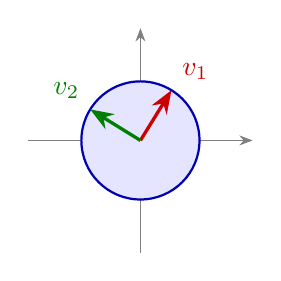
\begin{tikzpicture}[x=0.75cm, y=0.75cm, >=Stealth, baseline=(current bounding box.center)]
        \draw[->, gray] (-1.9,0) -- (1.9,0);
        \draw[->, gray] (0,-1.9) -- (0,1.9);
        \fill[blue!10] (0,0) circle (1);
        \draw[blue!70!black, thick] (0,0) circle (1);
        \draw[->, very thick, red!80!black] (0,0) -- (0.526,0.851) node[above right] {$v_1$};
        \draw[->, very thick, green!50!black] (0,0) -- (-0.851,0.526) node[above left] {$v_2$};
    \end{tikzpicture}
    $\xrightarrow{\ V^\top\ }$
    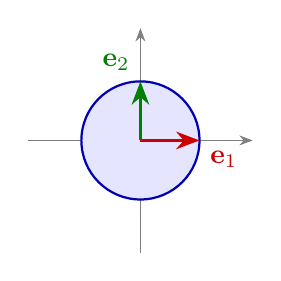
\begin{tikzpicture}[x=0.75cm, y=0.75cm, >=Stealth, baseline=(current bounding box.center)]
        \draw[->, gray] (-1.9,0) -- (1.9,0);
        \draw[->, gray] (0,-1.9) -- (0,1.9);
        \fill[blue!10] (0,0) circle (1);
        \draw[blue!70!black, thick] (0,0) circle (1);
        \draw[->, very thick, red!80!black] (0,0) -- (1,0) node[below right] {$\mathbf{e}_1$};
        \draw[->, very thick, green!50!black] (0,0) -- (0,1) node[above left] {$\mathbf{e}_2$};
    \end{tikzpicture}
    $\xrightarrow{\ \Sigma\ }$
    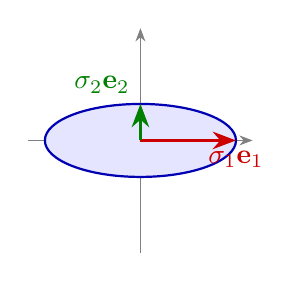
\begin{tikzpicture}[x=0.75cm, y=0.75cm, >=Stealth, baseline=(current bounding box.center)]
        \draw[->, gray] (-1.9,0) -- (1.9,0);
        \draw[->, gray] (0,-1.9) -- (0,1.9);
        \fill[blue!10] (0,0) ellipse [x radius=1.618, y radius=0.618];
        \draw[blue!70!black, thick] (0,0) ellipse [x radius=1.618, y radius=0.618];
        \draw[->, very thick, red!80!black] (0,0) -- (1.618,0) node[below] {$\sigma_1 \mathbf{e}_1$};
        \draw[->, very thick, green!50!black] (0,0) -- (0,0.618) node[above left] {$\sigma_2 \mathbf{e}_2$};
    \end{tikzpicture}
    $\xrightarrow{\ U\ }$
    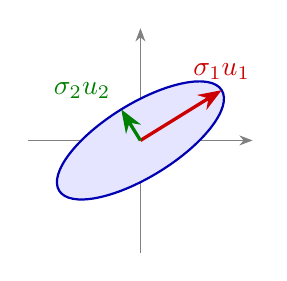
\begin{tikzpicture}[x=0.75cm, y=0.75cm, >=Stealth, baseline=(current bounding box.center)]
        \draw[->, gray] (-1.9,0) -- (1.9,0);
        \draw[->, gray] (0,-1.9) -- (0,1.9);
        \fill[blue!10, rotate=31.72] (0,0) ellipse [x radius=1.618, y radius=0.618];
        \draw[blue!70!black, thick, rotate=31.72] (0,0) ellipse [x radius=1.618, y radius=0.618];
        \draw[->, very thick, red!80!black] (0,0) -- (1.376,0.851) node[above] {$\sigma_1 u_1$};
        \draw[->, very thick, green!50!black] (0,0) -- (-0.325,0.526) node[above left] {$\sigma_2 u_2$};
    \end{tikzpicture}
    \caption[The geometry of the SVD]{The SVD of the shear $A = \begin{pmatrix} 1 & 1 \\ 0 & 1 \end{pmatrix}$ (Example~\ref{L2-ex:svd-shear}). The rotation $V^\top$ moves the right singular vectors $\mathbf{v}_1, \mathbf{v}_2$ to $\mathbf{e}_1, \mathbf{e}_2$; the scaling $\Sigma$ stretches the axes by $\sigma_1 = \varphi$ and $\sigma_2 = 1/\varphi$; and the rotation $U$ moves the axes to the left singular vectors. Altogether, the unit circle is mapped to an ellipse with semi-axes $\sigma_1 \mathbf{u}_1 = A\mathbf{v}_1$ and $\sigma_2 \mathbf{u}_2 = A\mathbf{v}_2$.}
    \label{L2-fig:svd}
\end{figure}

\begin{proposition}\label{L2-prop:svd-subspaces}
    Let $A = U\Sigma V^\top$ be an SVD of a matrix $A$ of rank $r$. Then
    \[A = \sigma_1 \mathbf{u}_1 \mathbf{v}_1^\top + \sigma_2 \mathbf{u}_2 \mathbf{v}_2^\top + \cdots + \sigma_r \mathbf{u}_r \mathbf{v}_r^\top,\]
    and the four fundamental subspaces of $A$ are
    \begin{align*}
        \col(A) &= \Span\{\mathbf{u}_1, \ldots, \mathbf{u}_r\}, & \Null(A^\top) &= \Span\{\mathbf{u}_{r+1}, \ldots, \mathbf{u}_m\}, \\
        \row(A) &= \Span\{\mathbf{v}_1, \ldots, \mathbf{v}_r\}, & \Null(A) &= \Span\{\mathbf{v}_{r+1}, \ldots, \mathbf{v}_n\}.
    \end{align*}
\end{proposition}

\begin{proof}
    For every $\mathbf{x}$, we saw in the proof of Theorem~\ref{L2-thm:svd} that $A\mathbf{x} = \sum_{i \leq r} \sigma_i \mathbf{u}_i (\mathbf{v}_i^\top \mathbf{x})$, which is the first formula applied to $\mathbf{x}$. The formula for $\col(A)$ was also shown there. If $\mathbf{x} = \sum_i c_i \mathbf{v}_i$, then $A\mathbf{x} = \sum_{i \leq r} \sigma_i c_i \mathbf{u}_i$, which is $\mathbf{0}$ if and only if $c_1 = \cdots = c_r = 0$; this gives $\Null(A)$. In an orthonormal basis, the orthogonal complement of the span of some basis vectors is the span of the other ones, so the remaining two formulas follow from Theorem~\ref{L2-thm:fundamental-subspaces} and Theorem~\ref{L2-thm:orth-decomposition}(3).
\end{proof}

The first formula writes $A$ as a sum of $r$ matrices of rank $1$. It also gives the reduced SVD $A = U_r \Sigma_r V_r^\top$, where $U_r$ and $V_r$ consist of the first $r$ columns of $U$ and $V$, and $\Sigma_r = \diag(\sigma_1, \ldots, \sigma_r)$; NumPy computes it with \py{np.linalg.svd(A, full_matrices=False)}.

\subsection{Matrix norms and low-rank approximation}

\begin{definition}[Spectral norm]
    The spectral norm (or operator norm) of an $m \times n$ matrix $A$ is
    \[\norm{A}_2 = \max_{\mathbf{x} \neq \mathbf{0}} \frac{\norm{A\mathbf{x}}}{\norm{\mathbf{x}}},\]
    the largest factor by which $A$ stretches a vector.
\end{definition}

\begin{proposition}\label{L2-prop:matrix-norms}
    Let $A$ have singular values $\sigma_1 \geq \cdots \geq \sigma_r > 0$. Then
    \[\norm{A}_2 = \sigma_1 \qquad \text{and} \qquad \norm{A}_F = \sqrt{\sigma_1^2 + \cdots + \sigma_r^2}.\]
\end{proposition}

\begin{proof}
    $\frac{\norm{A\mathbf{x}}^2}{\norm{\mathbf{x}}^2} = \frac{\mathbf{x}^\top A^\top A \mathbf{x}}{\mathbf{x}^\top \mathbf{x}}$ is the Rayleigh quotient of $A^\top A$, whose largest eigenvalue is $\sigma_1^2$; so the maximum is $\sigma_1$ by Proposition~\ref{L2-prop:rayleigh}. For the Frobenius norm, $\norm{A}_F^2 = \tr(A^\top A)$ is the sum of the eigenvalues of $A^\top A$ (by Lecture~1, the trace is the sum of the eigenvalues), which is $\sigma_1^2 + \cdots + \sigma_r^2$.
\end{proof}

The rank-$1$ expansion suggests approximating $A$ by keeping only the terms with the largest singular values. This is the best possible approximation of a given rank.

\begin{theorem}[Eckart--Young]\label{L2-thm:eckart-young}
    Let $A$ have the SVD $A = \sum_{i=1}^r \sigma_i \mathbf{u}_i \mathbf{v}_i^\top$, and for $k < r$ let
    \[A_k = \sigma_1 \mathbf{u}_1 \mathbf{v}_1^\top + \cdots + \sigma_k \mathbf{u}_k \mathbf{v}_k^\top.\]
    Then $\rank(A_k) = k$, and for every matrix $B$ of rank at most $k$,
    \[\norm{A - A_k}_2 = \sigma_{k+1} \leq \norm{A - B}_2 \qquad \text{and} \qquad \norm{A - A_k}_F = \sqrt{\sigma_{k+1}^2 + \cdots + \sigma_r^2} \leq \norm{A - B}_F.\]
\end{theorem}

\begin{proof}
    Since $A_k\mathbf{x} = \sum_{i \leq k} \sigma_i (\mathbf{v}_i^\top \mathbf{x}) \mathbf{u}_i$ for every $\mathbf{x}$, and $A_k\mathbf{v}_i = \sigma_i \mathbf{u}_i$ for $i \leq k$, the column space of $A_k$ is $\Span\{\mathbf{u}_1, \ldots, \mathbf{u}_k\}$, so $\rank(A_k) = k$. Moreover, $A - A_k = \sum_{i > k} \sigma_i \mathbf{u}_i \mathbf{v}_i^\top$ is an SVD of $A - A_k$, with the singular values $\sigma_{k+1}, \ldots, \sigma_r$, so the formulas for $\norm{A - A_k}_2$ and $\norm{A - A_k}_F$ follow from Proposition~\ref{L2-prop:matrix-norms}. Now let $\rank(B) \leq k$, and let $A$ be $m \times n$.

    \emph{Spectral norm.} By the rank--nullity theorem, $\dim\Null(B) \geq n - k$. The subspaces $\Null(B)$ and $\Span\{\mathbf{v}_1, \ldots, \mathbf{v}_{k+1}\}$ of $\mathbb{R}^n$ have dimensions adding up to more than $n$, so they have a nonzero vector in common: together, a basis of the first and a basis of the second contain more than $n$ vectors, so some nontrivial linear combination of them is $0$, and moving the terms of the second basis to the other side gives a vector $\mathbf{x}$ that lies in both subspaces; it is nonzero, since each basis is linearly independent. We may assume $\norm{\mathbf{x}} = 1$. Write $\mathbf{x} = \sum_{i \leq k+1} c_i \mathbf{v}_i$ with $\sum_i c_i^2 = 1$. Then $B\mathbf{x} = \mathbf{0}$ and $A\mathbf{x} = \sum_{i \leq k+1} \sigma_i c_i \mathbf{u}_i$, so
    \[\norm{A - B}_2^2 \geq \norm{(A - B)\mathbf{x}}^2 = \norm{A\mathbf{x}}^2 = \sum_{i=1}^{k+1} \sigma_i^2 c_i^2 \geq \sigma_{k+1}^2 \sum_{i=1}^{k+1} c_i^2 = \sigma_{k+1}^2.\]

    \emph{Frobenius norm.} Choose an orthonormal basis of $\col(B)$, which has at most $k$ vectors, and add vectors of an orthonormal basis of $\col(B)^\perp$ (Theorem~\ref{L2-thm:orth-decomposition}) until there are $k$ vectors; this is possible since $k < r \leq m$. Let $W$ be their span, and $C$ the $m \times k$ matrix with these columns, so that $C^\top C = I_k$, and $P = CC^\top$ is the matrix of the orthogonal projection onto $W \supseteq \col(B)$ (Proposition~\ref{L2-prop:projection-matrix}). For each column $\mathbf{a}_j$ of $A$ and $\mathbf{b}_j$ of $B$, we have $\mathbf{a}_j - \mathbf{b}_j = (P\mathbf{a}_j - \mathbf{b}_j) + (\mathbf{a}_j - P\mathbf{a}_j)$ with $P\mathbf{a}_j - \mathbf{b}_j \in W$ and $\mathbf{a}_j - P\mathbf{a}_j \in W^\perp$, so by Pythagoras,
    \[\norm{\mathbf{a}_j - \mathbf{b}_j}^2 \geq \norm{\mathbf{a}_j - P\mathbf{a}_j}^2 = \norm{\mathbf{a}_j}^2 - \norm{P\mathbf{a}_j}^2 = \norm{\mathbf{a}_j}^2 - \norm{C^\top \mathbf{a}_j}^2.\]
    Adding over $j$ gives $\norm{A - B}_F^2 \geq \norm{A}_F^2 - \norm{C^\top A}_F^2 = \norm{A}_F^2 - \tr(C^\top AA^\top C)$. The symmetric matrix $AA^\top = U\Sigma\Sigma^\top U^\top$ has the eigenvalues $\sigma_1^2 \geq \cdots \geq \sigma_r^2$, followed by zeros, so by Proposition~\ref{L2-prop:ky-fan}, $\tr(C^\top AA^\top C) \leq \sigma_1^2 + \cdots + \sigma_k^2$. Since $\norm{A}_F^2 = \sigma_1^2 + \cdots + \sigma_r^2$, we get $\norm{A - B}_F^2 \geq \sigma_{k+1}^2 + \cdots + \sigma_r^2$.
\end{proof}

\begin{example}\label{L2-ex:low-rank}
    Let $A = \begin{pmatrix} 3 & 0 \\ 4 & 5 \end{pmatrix}$. Then $A^\top A = \begin{pmatrix} 25 & 20 \\ 20 & 25 \end{pmatrix}$ has the eigenvalues $45$ and $5$, with eigenvectors $\mathbf{v}_1 = \frac{1}{\sqrt{2}}(1, 1)^\top$ and $\mathbf{v}_2 = \frac{1}{\sqrt{2}}(1, -1)^\top$. So $\sigma_1 = 3\sqrt{5}$, $\sigma_2 = \sqrt{5}$, and
    \[\mathbf{u}_1 = \frac{1}{3\sqrt{5}} A \mathbf{v}_1 = \frac{1}{\sqrt{10}} \begin{pmatrix} 1 \\ 3 \end{pmatrix}, \qquad \mathbf{u}_2 = \frac{1}{\sqrt{5}} A \mathbf{v}_2 = \frac{1}{\sqrt{10}} \begin{pmatrix} 3 \\ -1 \end{pmatrix}.\]
    The best rank-$1$ approximation of $A$ is
    \[A_1 = \sigma_1 \mathbf{u}_1 \mathbf{v}_1^\top = 3\sqrt{5} \cdot \frac{1}{\sqrt{20}} \begin{pmatrix} 1 \\ 3 \end{pmatrix} \begin{pmatrix} 1 & 1 \end{pmatrix} = \begin{pmatrix} 1.5 & 1.5 \\ 4.5 & 4.5 \end{pmatrix},\]
    with error $\norm{A - A_1}_F = \norm{A - A_1}_2 = \sigma_2 = \sqrt{5}$. Also, $\norm{A}_2 = 3\sqrt{5} \approx 6.71$.
\end{example}

\begin{remark}[Low-rank approximation in machine learning]
    A grayscale image with $m \times n$ pixels is an $m \times n$ matrix. Storing its rank-$k$ approximation $A_k$ requires only the $k(m + n + 1)$ numbers $\sigma_i$, $\mathbf{u}_i$, $\mathbf{v}_i$, instead of $mn$; for natural images, the singular values decay quickly, and a small $k$ already gives a good approximation (Programming Exercise~P10). The same idea is behind recommender systems, which approximate the matrix of user ratings by a low-rank matrix, latent semantic analysis of text, and the compression of large neural networks.
\end{remark}

\subsection{The pseudo-inverse}

\begin{definition}[Pseudo-inverse]
    Let $A = U\Sigma V^\top$ be an SVD of an $m \times n$ matrix $A$. The pseudo-inverse of $A$ is the $n \times m$ matrix
    \[A^+ = V \Sigma^+ U^\top,\]
    where $\Sigma^+$ is the $n \times m$ matrix with $(\Sigma^+)_{ii} = \frac{1}{\sigma_i}$ for $i \leq r$ and all other entries $0$.
\end{definition}

If $A$ is invertible, then $A^+ = A^{-1}$, since $A^{-1} = (U\Sigma V^\top)^{-1} = V\Sigma^{-1}U^\top$.

\begin{proposition}\label{L2-prop:pinv}
    If $A$ has linearly independent columns, then $A^+ = (A^\top A)^{-1} A^\top$, and $A^+ \mathbf{y}$ is the least squares solution of $A\mathbf{w} \approx \mathbf{y}$ (Theorem~\ref{L2-thm:least-squares}).
\end{proposition}

\begin{proof}
    In this case, $r = n$, and $A^\top A = V\Sigma^\top U^\top U \Sigma V^\top = V \diag(\sigma_1^2, \ldots, \sigma_n^2) V^\top$. Hence
    \[(A^\top A)^{-1} A^\top = V \diag(\sigma_1^{-2}, \ldots, \sigma_n^{-2}) V^\top V \Sigma^\top U^\top = V \diag(\sigma_1^{-2}, \ldots, \sigma_n^{-2}) \Sigma^\top U^\top = V \Sigma^+ U^\top.\]
    The second statement is Theorem~\ref{L2-thm:least-squares}.
\end{proof}

In general, when the columns of $A$ are dependent, the least squares problem has infinitely many solutions, and $A^+\mathbf{y}$ is the one with the smallest norm.

\begin{proposition}\label{L2-prop:pinv-min-norm}
    Let $A$ be an $m \times n$ matrix and $\mathbf{y} \in \mathbb{R}^m$. The vectors $\mathbf{w}$ that minimize $\norm{A\mathbf{w} - \mathbf{y}}$ are exactly the vectors $\mathbf{w} = A^+\mathbf{y} + \mathbf{v}$ with $\mathbf{v} \in \Null(A)$, and among them, $A^+\mathbf{y}$ is the only one with the smallest norm.
\end{proposition}

\begin{proof}
    Let $A = U\Sigma V^\top$, and write $\mathbf{z} = V^\top \mathbf{w}$ and $\mathbf{c} = U^\top \mathbf{y}$. Since $U^\top$ preserves lengths (Theorem~\ref{L2-thm:orthogonal}) and $U^\top A = \Sigma V^\top$,
    \[\norm{A\mathbf{w} - \mathbf{y}}^2 = \norm{U^\top(A\mathbf{w} - \mathbf{y})}^2 = \norm{\Sigma \mathbf{z} - \mathbf{c}}^2 = \sum_{i=1}^r (\sigma_i z_i - c_i)^2 + \sum_{i=r+1}^m c_i^2.\]
    This is smallest if and only if $z_i = c_i/\sigma_i$ for $i \leq r$, with $z_{r+1}, \ldots, z_n$ arbitrary. For $z_{r+1} = \cdots = z_n = 0$, this is $\mathbf{z} = \Sigma^+\mathbf{c}$, i.e., $\mathbf{w} = V\Sigma^+U^\top \mathbf{y} = A^+\mathbf{y}$. In general, $\mathbf{w} = V\mathbf{z} = A^+\mathbf{y} + \sum_{i > r} z_i\mathbf{v}_i$, and the vectors $\sum_{i > r} z_i\mathbf{v}_i$ are exactly the elements of $\Null(A)$ (Proposition~\ref{L2-prop:svd-subspaces}). Finally, $\norm{\mathbf{w}}^2 = \norm{\mathbf{z}}^2 = \sum_{i \leq r}(c_i/\sigma_i)^2 + \sum_{i > r} z_i^2$ is smallest exactly when $z_{r+1} = \cdots = z_n = 0$.
\end{proof}

NumPy's \py{np.linalg.pinv} and \py{np.linalg.lstsq} use the SVD in this way.

\subsection{Principal component analysis}\label{L2-sec:pca}

Principal component analysis (PCA) is the most widely used method to reduce the dimension of data. Let $\mathbf{x}_1, \ldots, \mathbf{x}_N \in \mathbb{R}^d$ be data points, which we assume to be centered, i.e., $\sum_i \mathbf{x}_i = \mathbf{0}$ (otherwise, subtract the mean from every data point first). Let $X$ be the $N \times d$ data matrix whose rows are $\mathbf{x}_1^\top, \ldots, \mathbf{x}_N^\top$, and let
\[S = \frac{1}{N} X^\top X = \frac{1}{N} \sum_{i=1}^N \mathbf{x}_i \mathbf{x}_i^\top\]
be the (sample) covariance matrix, which is symmetric positive semidefinite.

We look for a $k$-dimensional subspace $U$ such that the projected data points $\pi_U(\mathbf{x}_i)$ are as close as possible to the original ones, i.e., such that the reconstruction error $\sum_i \norm{\mathbf{x}_i - \pi_U(\mathbf{x}_i)}^2$ is as small as possible. By Pythagoras, $\norm{\mathbf{x}_i}^2 = \norm{\pi_U(\mathbf{x}_i)}^2 + \norm{\mathbf{x}_i - \pi_U(\mathbf{x}_i)}^2$, so equivalently, we look for the subspace for which the projected data has the largest spread $\sum_i \norm{\pi_U(\mathbf{x}_i)}^2$.

\begin{theorem}[PCA]\label{L2-thm:pca}
    Let $\mathbf{q}_1, \ldots, \mathbf{q}_d$ be orthonormal eigenvectors of $S$ with eigenvalues $\lambda_1 \geq \cdots \geq \lambda_d \geq 0$. Among all $k$-dimensional subspaces $U$ of $\mathbb{R}^d$, the reconstruction error is smallest for $U = \Span\{\mathbf{q}_1, \ldots, \mathbf{q}_k\}$, and then
    \[\frac{1}{N}\sum_{i=1}^N \norm{\mathbf{x}_i - \pi_U(\mathbf{x}_i)}^2 = \lambda_{k+1} + \cdots + \lambda_d.\]
\end{theorem}

\begin{proof}
    Let $\mathbf{b}_1, \ldots, \mathbf{b}_k$ be an orthonormal basis of $U$. Then $\pi_U(\mathbf{x}_i) = \sum_j (\mathbf{b}_j^\top \mathbf{x}_i) \mathbf{b}_j$, so $\norm{\pi_U(\mathbf{x}_i)}^2 = \sum_j (\mathbf{b}_j^\top \mathbf{x}_i)^2$ by Pythagoras, and
    \[\frac{1}{N}\sum_{i=1}^N \norm{\pi_U(\mathbf{x}_i)}^2 = \sum_{j=1}^k \frac{1}{N}\sum_{i=1}^N (\mathbf{b}_j^\top \mathbf{x}_i)^2 = \sum_{j=1}^k \frac{1}{N}\norm{X\mathbf{b}_j}^2 = \sum_{j=1}^k \mathbf{b}_j^\top S \mathbf{b}_j,\]
    which by Proposition~\ref{L2-prop:ky-fan} is at most $\lambda_1 + \cdots + \lambda_k$, with equality for $\mathbf{b}_j = \mathbf{q}_j$. For $k = 1$, this is just Proposition~\ref{L2-prop:rayleigh}. The error formula follows from Pythagoras, since $\frac{1}{N}\sum_i \norm{\mathbf{x}_i}^2 = \frac{1}{N}\tr(X^\top X) = \tr(S) = \lambda_1 + \cdots + \lambda_d$.
\end{proof}

The vectors $\mathbf{q}_1, \mathbf{q}_2, \ldots$ are called the principal components, or principal directions, of the data, and $\lambda_i = \mathbf{q}_i^\top S \mathbf{q}_i$ is the variance of the data in the direction $\mathbf{q}_i$. The fraction $\frac{\lambda_1 + \cdots + \lambda_k}{\lambda_1 + \cdots + \lambda_d}$ is the proportion of the variance explained by the first $k$ principal components. In practice, PCA is computed with the SVD of the data matrix: if $X = \tilde{U} \tilde{\Sigma} \tilde{V}^\top$, then
\[S = \frac{1}{N} X^\top X = \tilde{V}\, \frac{\tilde{\Sigma}^\top \tilde{\Sigma}}{N}\, \tilde{V}^\top,\]
so the principal components are the right singular vectors of $X$, and $\lambda_i = \sigma_i^2 / N$. The coordinates of the data in the principal directions are the entries of $X\tilde{V}$.

\begin{example}\label{L2-ex:pca}
    Consider the four centered data points $(2, 2)$, $(-2, -2)$, $(1, -1)$ and $(-1, 1)$ in $\mathbb{R}^2$. Then
    \[X^\top X = \begin{pmatrix} 10 & 6 \\ 6 & 10 \end{pmatrix}, \qquad S = \frac{1}{4} X^\top X = \begin{pmatrix} 2.5 & 1.5 \\ 1.5 & 2.5 \end{pmatrix},\]
    with eigenvalues $4$ and $1$ and eigenvectors $\mathbf{q}_1 = \frac{1}{\sqrt{2}}(1, 1)^\top$ and $\mathbf{q}_2 = \frac{1}{\sqrt{2}}(1, -1)^\top$. The first principal component explains $\frac{4}{4 + 1} = 80\%$ of the variance. Projecting onto $\Span\{\mathbf{q}_1\}$ keeps the first two points, and maps the last two to $\mathbf{0}$; the average reconstruction error is $\frac{1}{4}(0 + 0 + 2 + 2) = 1 = \lambda_2$, as predicted by Theorem~\ref{L2-thm:pca}.
\end{example}

\section{Key Takeaways}
\begin{itemize}[leftmargin=*]
    \item A norm measures length: it is positive definite, absolutely homogeneous, and satisfies the triangle inequality. Important examples on $\mathbb{R}^n$ are the $\ell_1$, $\ell_2$ and $\ell_\infty$ norms, whose unit balls are a diamond, a ball and a cube.
    \item An inner product is a symmetric, positive definite, bilinear function. On an $n$-dimensional space with a fixed basis, inner products correspond to symmetric positive definite matrices: $\ip{\mathbf{x}}{\mathbf{y}} = \mathbf{x}^\top A \mathbf{y}$.
    \item Every inner product induces a norm $\norm{x} = \sqrt{\ip{x}{x}}$ and a distance $d(x, y) = \norm{x - y}$. The Cauchy--Schwarz inequality $|\ip{x}{y}| \leq \norm{x}\norm{y}$ gives the triangle inequality and allows us to define angles by $\cos\omega = \frac{\ip{x}{y}}{\norm{x}\norm{y}}$.
    \item Vectors are orthogonal if their inner product is $0$. Orthogonal matrices ($Q^\top Q = I$) are exactly the matrices that preserve dot products, lengths and angles.
    \item In an orthonormal basis, coordinates are inner products: $v = \sum_i \ip{v}{b_i} b_i$. The Gram--Schmidt process turns any basis into an orthonormal basis, and gives the QR decomposition.
    \item Every subspace $U$ of a finite-dimensional inner product space has an orthogonal complement with $V = U \oplus U^\perp$. For a matrix, $\Null(A) = \row(A)^\perp$ and $\Null(A^\top) = \col(A)^\perp$.
    \item A hyperplane $\{\mathbf{x} : \mathbf{w}^\top \mathbf{x} = c\}$ has normal vector $\mathbf{w}$; linear classifiers use hyperplanes as decision boundaries, and the distance of $\mathbf{x}$ to the hyperplane is $\frac{|\mathbf{w}^\top \mathbf{x} - c|}{\norm{\mathbf{w}}}$.
    \item The orthogonal projection onto $U = \col(B)$ is $\pi_U(\mathbf{x}) = B(B^\top B)^{-1}B^\top \mathbf{x}$; it is the point of $U$ closest to $\mathbf{x}$. Least squares regression projects the target vector onto the column space of the design matrix, which leads to the normal equations $A^\top A \mathbf{w} = A^\top \mathbf{y}$.
    \item Rotations are orthogonal matrices with determinant $1$. They preserve lengths, angles and orientation; rotations of the plane commute, but rotations of $\mathbb{R}^3$ do not.
    \item Spectral theorem: a symmetric matrix has real eigenvalues and an orthonormal basis of eigenvectors, $A = Q\Lambda Q^\top = \sum_i \lambda_i \mathbf{q}_i \mathbf{q}_i^\top$. It is positive definite if and only if all eigenvalues are positive, and $\max_{\norm{\mathbf{x}} = 1} \mathbf{x}^\top A \mathbf{x} = \lambda_{\max}$.
    \item The Laplacian $L = D - W$ of a weighted graph satisfies $\mathbf{x}^\top L\mathbf{x} = \sum_{i < j} w_{ij}(x_i - x_j)^2$, so it is positive semidefinite. The multiplicity of its eigenvalue $0$ is the number of connected components, and its second smallest eigenvalue $\lambda_2$ is a lower bound for the ratio cut of every split of the vertices. Spectral clustering splits the vertices by the signs of the Fiedler vector $\mathbf{q}_2$.
    \item Every matrix has a singular value decomposition $A = U\Sigma V^\top = \sum_{i=1}^r \sigma_i \mathbf{u}_i \mathbf{v}_i^\top$: rotate, scale the axes by the singular values, rotate. The $\sigma_i^2$ are the eigenvalues of $A^\top A$, $r = \rank(A)$, $\norm{A}_2 = \sigma_1$ and $\norm{A}_F^2 = \sum_i \sigma_i^2$.
    \item Keeping the $k$ largest singular values gives the best rank-$k$ approximation (Eckart--Young), with applications to compression and recommender systems. PCA projects centered data onto the eigenvectors of the covariance matrix with the largest eigenvalues, i.e., onto the top right singular vectors of the data matrix.
\end{itemize}

\section{Exercises}\label{L2-sec:exercises}
\begin{enumerate}[leftmargin=*]
    \item Let $\mathbf{x} = (1, -2, 2)^\top$ and $\mathbf{y} = (3, 0, 1)^\top$. Compute $\norm{\mathbf{x}}_1$, $\norm{\mathbf{x}}_2$ and $\norm{\mathbf{x}}_\infty$, and the distance between $\mathbf{x}$ and $\mathbf{y}$ in each of the three norms.
    \item Show that $\norm{\mathbf{x}}_2 \leq \sqrt{n}\, \norm{\mathbf{x}}_\infty$ for all $\mathbf{x} \in \mathbb{R}^n$. For which vectors $\mathbf{x}$ does equality hold in $\norm{\mathbf{x}}_1 \leq \sqrt{n}\, \norm{\mathbf{x}}_2$?
    \item Show that the $\ell_\infty$ norm on $\mathbb{R}^2$ does not satisfy the parallelogram law, and conclude that it does not come from an inner product.
    \item Which of the following matrices are symmetric positive definite? For each one that is, write down the corresponding inner product $\ip{\mathbf{x}}{\mathbf{y}} = \mathbf{x}^\top A \mathbf{y}$ on $\mathbb{R}^2$ explicitly.
    \[\begin{pmatrix} 2 & 1 \\ 1 & 2 \end{pmatrix}, \qquad \begin{pmatrix} 1 & 2 \\ 2 & 1 \end{pmatrix}, \qquad \begin{pmatrix} 1 & 0 \\ 0 & 0 \end{pmatrix}, \qquad \begin{pmatrix} 4 & -2 \\ -2 & 1 \end{pmatrix}, \qquad \begin{pmatrix} 3 & 1 \\ 1 & 1 \end{pmatrix}.\]
    \item Find the angle between the vectors: (a) $(1, 1, 0)^\top$ and $(1, 0, 1)^\top$; (b) $(1, 2, 3)^\top$ and $(-3, 0, 1)^\top$; (c) $(1, 0)^\top$ and $(-1, \sqrt{3})^\top$.
    \item \begin{enumerate}[label=(\alph*)]
        \item Find all vectors in $\mathbb{R}^3$ that are orthogonal to both $(1, 1, 1)^\top$ and $(1, -1, 1)^\top$. (Hint: this is the null space of a matrix.)
        \item The planes $x + y + z = 3$ and $x - y + z = 5$ intersect in a line $\ell$. Find an equation of the plane through the origin that is perpendicular to $\ell$.
    \end{enumerate}
    \item Apply the Gram--Schmidt process to $\mathbf{v}_1 = (1, 2, 2)^\top$ and $\mathbf{v}_2 = (1, 0, 1)^\top$. Then find a third vector that extends the result to an orthonormal basis of $\mathbb{R}^3$, and write $(1, 1, 1)^\top$ in this basis. Check Parseval's identity.
    \item Find a basis of the orthogonal complement of $U = \Span\{(1, 0, 1, 0)^\top, (0, 1, 0, 1)^\top\}$ in $\mathbb{R}^4$.
    \item Let $\mathbf{x} = (1, 0, 2)^\top$. Compute the orthogonal projection of $\mathbf{x}$ onto (a) the line spanned by $(1, 1, 0)^\top$, and (b) the plane $x_1 + x_2 + x_3 = 0$. Write down the projection matrices of both projections.
    \item Find the point of the plane $2x + y + 3z = 3$ that is closest to the origin, and the distance from the origin to this plane.
    \item Let $P$ be a symmetric $n \times n$ matrix with $P^2 = P$. Show that $P$ is the matrix of the orthogonal projection onto $\col(P)$. (Hint: show that $\mathbf{x} - P\mathbf{x} \in \col(P)^\perp = \Null(P^\top)$.)
    \item Let $\mathbf{u} \in \mathbb{R}^n$ be a unit vector, and let $H = I_n - 2\mathbf{u}\mathbf{u}^\top$.
    \begin{enumerate}[label=(\alph*)]
        \item Show that $H$ is symmetric and orthogonal, and that $H^2 = I_n$.
        \item Show that $H\mathbf{u} = -\mathbf{u}$, and that $H\mathbf{x} = \mathbf{x}$ for every $\mathbf{x} \perp \mathbf{u}$. Describe $H$ geometrically. (Such matrices are called Householder reflections; \py{np.linalg.qr} uses them.)
    \end{enumerate}
    \item\label{L2-ex2:best-poly} Find the polynomial $p$ of degree at most $1$ that minimizes $\int_{-1}^1 \big(x^3 - p(x)\big)^2 \, dx$, by projecting $x^3$ onto $\Span\{1, x\}$ in $C[-1, 1]$. Compare with Example~\ref{L2-ex:legendre}.
    \item Find the least squares line for the data points $(0, 1)$, $(1, 1)$ and $(2, 3)$, and check that the residual vector is orthogonal to the columns of the design matrix.
    \item Show that the product of two orthogonal $2 \times 2$ matrices with determinant $-1$ (for example, two reflections) is a rotation. Compute $R_1(\theta)^\top R_1(\theta)$ and $\det R_1(\theta)$.
    \item Use the Cauchy--Schwarz inequality to show that $(x_1 + \cdots + x_n)^2 \leq n(x_1^2 + \cdots + x_n^2)$. Conclude that if $a, b, c \geq 0$ and $a + b + c = 1$, then $a^2 + b^2 + c^2 \geq \frac{1}{3}$. When does equality hold?
    \item Find the spectral decomposition $A = Q\Lambda Q^\top$ of $A = \begin{pmatrix} 5 & 2 \\ 2 & 2 \end{pmatrix}$, and write $A$ as $\lambda_1 \mathbf{q}_1 \mathbf{q}_1^\top + \lambda_2 \mathbf{q}_2 \mathbf{q}_2^\top$. Is $A$ positive definite? Conversely, show that every matrix of the form $Q\Lambda Q^\top$, with $Q$ orthogonal and $\Lambda$ diagonal, is symmetric.
    \item Find the largest and the smallest value of $\mathbf{x}^\top A \mathbf{x}$ over all unit vectors $\mathbf{x} \in \mathbb{R}^2$, for $A = \begin{pmatrix} 2 & 1 \\ 1 & 2 \end{pmatrix}$, and the unit vectors where they are attained.
    \item Let $L$ be the Laplacian of a graph with weights $w_{ij}$.
    \begin{enumerate}
        \item Show that $L = \sum_{i < j} w_{ij}(\mathbf{e}_i - \mathbf{e}_j)(\mathbf{e}_i - \mathbf{e}_j)^\top$, and use this to give another proof of Proposition~\ref{L2-prop:laplacian}.
        \item Find the Laplacian and its eigenvalues for the star graph with the center $1$ and the leaves $2, \ldots, n$, where $n \geq 3$ and all weights are $1$. (Hint: consider the vectors with $x_1 = 0$ whose entries add up to $0$, and the vector $(n - 1, -1, \ldots, -1)^\top$.) Why is the Fiedler vector not unique, and what does this say about clusters in a star?
    \end{enumerate}
    \item Compute an SVD of (a) $\begin{pmatrix} 0 & 2 \\ 1 & 0 \end{pmatrix}$ and (b) $\begin{pmatrix} 2 & 2 \\ 1 & 1 \end{pmatrix}$. For (b), write $A$ as $\sigma_1 \mathbf{u}_1 \mathbf{v}_1^\top$, and compute the pseudo-inverse $A^+$.
    \item Show that:
    \begin{enumerate}[label=(\alph*)]
        \item all singular values of an orthogonal matrix are equal to $1$;
        \item the singular values of a symmetric matrix are the absolute values of its nonzero eigenvalues;
        \item $A^\top A$ and $AA^\top$ have the same nonzero eigenvalues;
        \item $\norm{A}_2 = \norm{A^\top}_2$.
    \end{enumerate}
    \item Carry out PCA by hand for the four data points $(3, 3)$, $(-3, -3)$, $(1, -1)$, $(-1, 1)$: compute the covariance matrix, the principal components, and the proportion of the variance explained by the first principal component. Project the data onto the first principal component, and compute the average reconstruction error.
\end{enumerate}

\section{Programming Exercises}\label{L2-sec:programming}

% Inline code cannot be hyphenated, so allow a little extra stretch in this section.
\setlength{\emergencystretch}{3em}

As in Lecture~1, implement the algorithms yourself with NumPy, and use NumPy's built-in routines only to check your results. You need Matplotlib for P1, P5, P7, P10 and P11. Start each file with
\begin{lstlisting}
import numpy as np
rng = np.random.default_rng(0)  # random number generator for test data
\end{lstlisting}

\begin{enumerate}[label=\textbf{P\arabic*.}, leftmargin=*]
    \item \textbf{Norms and unit balls.} Write a function \py{p_norm(x, p)} for $p \geq 1$ and $p = \infty$ (use \py{np.inf}), and compare it with \py{np.linalg.norm(x, ord=p)}.
    \begin{itemize}
        \item For $10\,000$ random vectors in $\mathbb{R}^5$, check the inequalities $\norm{\mathbf{x}}_\infty \leq \norm{\mathbf{x}}_2 \leq \norm{\mathbf{x}}_1 \leq \sqrt{5}\, \norm{\mathbf{x}}_2$.
        \item Plot the unit circles $\{\mathbf{x} \in \mathbb{R}^2 : \norm{\mathbf{x}}_p = 1\}$ for $p = 1, 1.5, 2, 4, \infty$ in one picture, as in Figure~\ref{L2-fig:unit-balls}. (Hint: for each angle $t$, rescale the vector $(\cos t, \sin t)$ to have $p$-norm $1$.)
    \end{itemize}

    \item \textbf{Inner products and angles.} Write a function \py{inner(x, y, A)} that computes $\mathbf{x}^\top A \mathbf{y}$, and functions \py{norm_A(x, A)} and \py{angle_A(x, y, A)} for the induced norm and angle.
    \begin{itemize}
        \item Check Example~\ref{L2-ex:orth-depends}: the angle between $(1, 1)$ and $(-1, 1)$ is $90^\circ$ for $A = I_2$, but about $109.5^\circ$ for $A = \diag(2, 1)$.
        \item Write a function \py{is_spd(A)} that tests whether a symmetric $2 \times 2$ matrix is positive definite, using Proposition~\ref{L2-prop:spd-properties}. For larger matrices, NumPy's \py{np.linalg.cholesky(A)} succeeds exactly for symmetric positive definite matrices and raises \py{np.linalg.LinAlgError} otherwise; use it to test the matrices of Exercise~4.
        \item For random vectors, check the Cauchy--Schwarz inequality, and the parallelogram law for the $\ell_2$ norm (but not for the $\ell_1$ norm).
    \end{itemize}

    \item \textbf{Gram--Schmidt, and how it can fail.} Implement the classical Gram--Schmidt process \py{gram_schmidt(V)}, which returns a matrix $Q$ whose columns are the orthonormal vectors obtained from the columns of \py{V}, exactly as in Theorem~\ref{L2-thm:gram-schmidt}.
    \begin{itemize}
        \item Check your function on Example~\ref{L2-ex:gram-schmidt}, and compute $R = Q^\top V$; it should be upper triangular, with $V = QR$.
        \item The modified Gram--Schmidt process subtracts the components one at a time, from the updated vector: for each $i < j$, replace $\mathbf{u}_j$ by $\mathbf{u}_j - \ip{\mathbf{u}_j}{\mathbf{e}_i} \mathbf{e}_i$. In exact arithmetic, both versions give the same result. Implement it as well.
        \item For the Hilbert matrices $H_n$ with entries $\frac{1}{i + j - 1}$ (whose columns are nearly linearly dependent) and $n = 6, 8, 10, 12$, compute the loss of orthogonality \py{np.linalg.norm(Q.T @ Q - np.eye(n))} for the classical version, the modified version, and \py{np.linalg.qr}. What do you observe?
    \end{itemize}

    \item \textbf{Projections.} Write a function \py{project(x, B)} that returns the orthogonal projection of $\mathbf{x}$ onto the column space of \py{B}, by solving the normal equations, and a function \py{projection_matrix(B)}.
    \begin{itemize}
        \item Check your functions on Example~\ref{L2-ex:projection-plane}.
        \item For a random $6 \times 3$ matrix $B$ and a random $\mathbf{x} \in \mathbb{R}^6$, check that $P^2 = P$, $P^\top = P$, and that $\mathbf{x} - P\mathbf{x}$ is orthogonal to every column of $B$.
        \item Check Theorem~\ref{L2-thm:best-approximation} numerically: compare $\norm{\mathbf{x} - P\mathbf{x}}$ with $\norm{\mathbf{x} - B\boldsymbol{\lambda}}$ for $1000$ random vectors $\boldsymbol{\lambda} \in \mathbb{R}^3$.
        \item Orthonormalize the columns of $B$ with your function from P3, and check that $QQ^\top$ is the same projection matrix.
    \end{itemize}

    \item \textbf{Polynomial regression.} Generate $20$ noisy data points
\begin{lstlisting}
x = np.linspace(-1, 1, 20)
y = np.sin(3 * x) + rng.normal(0, 0.1, size=20)
\end{lstlisting}
    \begin{itemize}
        \item For $d = 1, 3, 5, 15$, fit a polynomial of degree $d$ by least squares: build the design matrix with columns $1, x, \ldots, x^d$ and solve the normal equations. Compare your coefficients with \py{np.linalg.lstsq}.
        \item Plot the data and the four fitted polynomials. Which degree fits the training data best? Which one would you trust for new data? (This is the phenomenon of overfitting.)
        \item Check that for each $d$, the residual vector is orthogonal to all columns of the design matrix.
    \end{itemize}

    \item \textbf{Nearest neighbors with different metrics.} Generate two classes of points in $\mathbb{R}^2$:
\begin{lstlisting}
X0 = rng.normal([0, 0], [1.0, 0.3], size=(100, 2))   # class 0
X1 = rng.normal([1.5, 1.0], [1.0, 0.3], size=(100, 2))  # class 1
\end{lstlisting}
    and split the $200$ points randomly into $150$ training points and $50$ test points.
    \begin{itemize}
        \item Implement the $1$-nearest neighbor classifier with the $\ell_1$, $\ell_2$ and $\ell_\infty$ distances, and with the cosine similarity (largest similarity instead of smallest distance). Compare their accuracies on the test points.
        \item Multiply the second coordinate of all points by $1000$ (as if it were measured in different units) and repeat. What happens to the accuracies of the distance-based and the cosine-based classifiers, and why? What happens if you standardize each feature (subtract its mean, divide by its standard deviation) first?
        \item Rotate all points by a random rotation $R_\theta$ and repeat. Which classifiers give exactly the same predictions, and why?
    \end{itemize}

    \item \textbf{Rotations.} Write functions \py{R1(t)}, \py{R2(t)} and \py{R3(t)} that return the rotation matrices of Section~\ref{L2-sec:rotations}, and a function \py{givens(n, i, j, t)}.
    \begin{itemize}
        \item Check that all of them are orthogonal with determinant $1$, and that they preserve the lengths of random vectors.
        \item Check that \py{R1(t) @ R3(s)} and \py{R3(s) @ R1(t)} differ for most angles, while \py{R3(t) @ R3(s)} equals \py{R3(t + s)}.
        \item Let \py{Q, R = np.linalg.qr(rng.normal(size=(3, 3)))}. Then \py{Q} is orthogonal, but its determinant may be $-1$. How can you turn it into a rotation by changing the sign of one column? Generate many random rotations this way, apply them to $\mathbf{e}_3$, and plot the resulting points on the sphere (Matplotlib can make 3D scatter plots).
    \end{itemize}

    \item \textbf{The perceptron and its margin.} The perceptron algorithm learns a linear classifier $f(\mathbf{x}) = \sign(\mathbf{w}^\top \mathbf{x} + b)$ from labeled data $(\mathbf{x}_i, y_i)$ with $y_i \in \{+1, -1\}$: start with $\mathbf{w} = \mathbf{0}$ and $b = 0$, and repeatedly go through the data; whenever a point is misclassified, i.e., $y_i (\mathbf{w}^\top \mathbf{x}_i + b) \leq 0$, update $\mathbf{w} \leftarrow \mathbf{w} + y_i \mathbf{x}_i$ and $b \leftarrow b + y_i$. Stop when all points are classified correctly.
    \begin{itemize}
        \item Generate linearly separable data, e.g., $50$ points on each side of the line $\mathbf{x}_1 + \mathbf{x}_2 = 2$ (discard points that are closer than $0.2$ to the line), and run the perceptron.
        \item Using Theorem~\ref{L2-thm:distance-hyperplane}, compute the margin of the learned classifier, i.e., the smallest distance of a training point to the decision boundary. Compare it with the margin of the classifier $\mathbf{w} = (1, 1)$, $b = -2$.
        \item Count the number of updates the perceptron needs. How does it change when you discard points closer than $0.5$ (instead of $0.2$) to the line?
    \end{itemize}

    \item \textbf{The spectral theorem in practice.} For symmetric matrices, use \py{np.linalg.eigh}, which returns real eigenvalues in increasing order and orthonormal eigenvectors.
    \begin{itemize}
        \item For a random symmetric matrix \py{A = B + B.T} (with \py{B = rng.normal(size=(5, 5))}), check that \py{Q.T @ Q} is close to $I_5$ and that \py{Q @ np.diag(lam) @ Q.T} is close to $A$. Check the spectral decomposition $A = \sum_i \lambda_i \mathbf{q}_i \mathbf{q}_i^\top$ as well.
        \item Write a function \py{is_spd(A)} based on Corollary~\ref{L2-cor:spd-eigenvalues}, and compare it with your test from P2.
        \item Check Proposition~\ref{L2-prop:rayleigh} numerically: evaluate the Rayleigh quotient $\frac{\mathbf{x}^\top A \mathbf{x}}{\mathbf{x}^\top \mathbf{x}}$ at $10\,000$ random vectors, and compare the largest and smallest values you find with the largest and smallest eigenvalues.
    \end{itemize}

    \item \textbf{Image compression with the SVD.} Load a grayscale image as a 2D array \py{A}, for example with \py{A = plt.imread("photo.png").mean(axis=2)} for a color image (with \py{import matplotlib.pyplot as plt}), or create one, e.g., from the function $\sin(x)\cos(y) + \frac{x}{10}$ on a $200 \times 300$ grid plus some noise.
    \begin{itemize}
        \item Compute \py{U, s, Vt = np.linalg.svd(A, full_matrices=False)} and plot the singular values on a logarithmic scale. How fast do they decay?
        \item For $k = 1, 5, 20, 50$, compute the rank-$k$ approximation $A_k$ (Theorem~\ref{L2-thm:eckart-young}) and display it as an image. Compare \py{np.linalg.norm(A - A_k)} with $\sqrt{\sigma_{k+1}^2 + \cdots + \sigma_r^2}$, and compute the storage ratio $\frac{k(m + n + 1)}{mn}$.
        \item Check numerically that $\norm{A}_2 = \sigma_1$ (\py{np.linalg.norm(A, 2)}) and $\norm{A}_F^2 = \sum_i \sigma_i^2$.
    \end{itemize}

    \item \textbf{Principal component analysis.} Generate $500$ data points from a correlated Gaussian distribution:
\begin{lstlisting}
C = np.array([[3.0, 1.5], [1.5, 1.0]])  # covariance matrix
X = rng.multivariate_normal([2, -1], C, size=500)
\end{lstlisting}
    \begin{itemize}
        \item Center the data, and compute the principal components in two ways: as eigenvectors of the covariance matrix $S = \frac{1}{N}X^\top X$ (with \py{np.linalg.eigh}), and as right singular vectors of $X$ (with \py{np.linalg.svd}). Check that they agree (up to sign), and that $\lambda_i = \sigma_i^2 / N$. How do they compare with the eigenvectors of $C$?
        \item Plot the data together with the two principal directions, scaled by $\sqrt{\lambda_i}$. What proportion of the variance does the first principal component explain?
        \item Project the data onto the first principal component, plot the projected points, and check that the average reconstruction error is $\lambda_2$ (Theorem~\ref{L2-thm:pca}).
        \item Generate $500$ points in $\mathbb{R}^{10}$ that lie close to a $2$-dimensional subspace, for example
\begin{lstlisting}
X = rng.normal(size=(500, 2)) @ rng.normal(size=(2, 10))
X = X + 0.05 * rng.normal(size=(500, 10))  # small noise
\end{lstlisting}
        Plot the $10$ eigenvalues of the covariance matrix. How can you see from this plot that the data is essentially $2$-dimensional?
    \end{itemize}

    \item \textbf{Spectral clustering.} Generate $100$ points on each of two concentric circles with the radii $1$ and $3$:
\begin{lstlisting}
t = rng.uniform(0, 2 * np.pi, 200)
r = np.repeat([1.0, 3.0], 100)
X = np.c_[r * np.cos(t), r * np.sin(t)] + 0.1 * rng.normal(size=(200, 2))
\end{lstlisting}
    \begin{itemize}
        \item Build the weights $w_{ij} = e^{-\norm{\mathbf{x}_i - \mathbf{x}_j}^2/(2s^2)}$ with $s = 0.5$ (and $w_{ii} = 0$), the Laplacian $L$ (Definition~\ref{L2-def:laplacian}), and its eigenvalues and eigenvectors with \py{np.linalg.eigh}. Check that the smallest eigenvalue is $0$, with the eigenvector $\frac{1}{\sqrt{n}}\mathbf{1}$ (up to sign).
        \item Cluster the points by the signs of the Fiedler vector, and plot them in two colors. Does spectral clustering find the two circles? Why would a method that only splits the plane by a line fail here?
        \item Repeat with $s = 2$ and $s = 0.2$. How do the second and third smallest eigenvalues change, and how does the clustering change? Relate your observations to Theorem~\ref{L2-thm:laplacian-components}.
    \end{itemize}
\end{enumerate}
\endgroup

% Generated by make_book.py from Lecture3/lecture3.tex; edit the lecture, not this file.
\chapter{Vector Calculus and Optimization}\label{L3-chapter}
% The group keeps settings such as \emergencystretch inside the chapter.
\begingroup
\section*{Introduction}
\addcontentsline{toc}{section}{Introduction}

Almost every machine learning model is trained by solving an optimization problem. A model has parameters, such as the weights of a linear model or the millions of weights of a neural network, which we collect in a vector $\boldsymbol{\theta}$. A loss function $L(\boldsymbol{\theta})$ measures how badly the model with these parameters fits the training data, and training means finding parameters with a small loss. There are far too many parameters to try out all possible values. Instead, we start with some parameters and improve them step by step, and for this we need to know how the loss changes when we change the parameters slightly. This information is contained in the derivative of $L$. Vector calculus is the study of derivatives and integrals of functions of several variables. In this lecture:
\begin{itemize}
    \item we extend the derivative to functions $f: \mathbb{R}^n \to \mathbb{R}^m$: partial derivatives, gradients and Jacobian matrices;
    \item we prove the chain rule, which says that the derivative of a composition of functions is the product of their Jacobian matrices; it is the basis of backpropagation, the algorithm that computes the gradients of neural networks;
    \item we compute gradients with respect to vectors and matrices, such as the weight matrices of a neural network;
    \item we use second derivatives (the Hessian matrix) and Taylor's theorem to describe the shape of a function near a point;
    \item we apply all of this to optimization: critical points, gradient descent, Newton's method, convexity, and optimization with constraints (Lagrange multipliers);
    \item we study vector fields with their divergence and curl, and integrals over regions of $\mathbb{R}^n$: Fubini's theorem, the change of variables formula, line integrals, and the divergence theorem, which leads to integration by parts in $\mathbb{R}^n$; these are the tools for probability densities in Lecture~4, for generative models, and for the differential equations of Lecture~5.
\end{itemize}
We use the linear algebra of Lectures~1 and~2 throughout: derivatives are linear maps, given by matrices; the direction of steepest ascent comes from the Cauchy--Schwarz inequality; and the shape of a function near a minimum is described by the eigenvalues of a symmetric matrix. Some results from analysis, such as the existence of maxima on closed and bounded sets and the implicit function theorem, are only stated here; Appendix~\ref{A-chapter} on topology and differential topology proves them and puts them in a wider context.

\paragraph{Notation.} In this lecture, vectors are written in bold, $\mathbf{x} = (x_1, \ldots, x_n)^\top \in \mathbb{R}^n$, to distinguish them from numbers. As before, vectors are columns, $\mathbf{e}_1, \ldots, \mathbf{e}_n$ is the standard basis of $\mathbb{R}^n$, $\norm{\cdot}$ is the Euclidean norm, and $\log$ is the natural logarithm.

\section{Multivariable Functions}

\begin{definition}\label{L3-def:multivariable}
    A function $f: \mathbb{R}^n \to \mathbb{R}^m$ is a mapping that takes an input vector $\mathbf{x} \in \mathbb{R}^n$ and produces an output vector $\mathbf{y} = f(\mathbf{x}) \in \mathbb{R}^m$.
    The components of the output vector are given by $y_i = f_i(\mathbf{x})$ for $i = 1, 2, \ldots, m$, where each $f_i: \mathbb{R}^n \to \mathbb{R}$ is a scalar-valued function.
\end{definition}

\begin{example}\label{L3-ex:paraboloid}
    $f(x, y) = x^2 + y^2$ is a function from $\mathbb{R}^2$ to $\mathbb{R}$, which takes a point $(x, y)$ in the plane and maps it to the sum of the squares of its coordinates.
\end{example}

\begin{example}[Functions in machine learning]\label{L3-ex:ml-functions}
    \begin{enumerate}
        \item A linear model with weight vector $\mathbf{w} \in \mathbb{R}^n$ and bias $b \in \mathbb{R}$ is the function $f: \mathbb{R}^n \to \mathbb{R}$, $f(\mathbf{x}) = \mathbf{w}^\top \mathbf{x} + b$.
        \item A layer of a neural network is a function $f: \mathbb{R}^n \to \mathbb{R}^m$, $f(\mathbf{x}) = \sigma(W\mathbf{x} + \mathbf{b})$, where $W \in \mathbb{R}^{m \times n}$ is a weight matrix, $\mathbf{b} \in \mathbb{R}^m$ is a bias vector, and an activation function $\sigma: \mathbb{R} \to \mathbb{R}$ is applied to each entry of $W\mathbf{x} + \mathbf{b}$. Common activation functions are the sigmoid function $\sigma(t) = \frac{1}{1 + e^{-t}}$, the hyperbolic tangent $\tanh$, and the rectified linear unit $\ReLU(t) = \max(0, t)$.
        \item The softmax function $\softmax: \mathbb{R}^K \to \mathbb{R}^K$,
        \[\softmax(\mathbf{z})_i = \frac{e^{z_i}}{e^{z_1} + \cdots + e^{z_K}}, \qquad i = 1, \ldots, K,\]
        turns a vector of scores $\mathbf{z}$ into a vector of probabilities: its entries are positive and sum to $1$. Classifiers with $K$ classes use it to predict the probability of each class.
        \item Given training data $(\mathbf{x}_1, y_1), \ldots, (\mathbf{x}_N, y_N)$ with $\mathbf{x}_i \in \mathbb{R}^n$ and $y_i \in \mathbb{R}$, the mean squared error of a linear model without bias,
        \[L(\mathbf{w}) = \frac{1}{N} \sum_{i=1}^N (\mathbf{w}^\top \mathbf{x}_i - y_i)^2,\]
        is a function $L: \mathbb{R}^n \to \mathbb{R}$ of the weights.
    \end{enumerate}
\end{example}

The last example shows an important change of perspective. When we use a model, its parameters are fixed and the input $\mathbf{x}$ is the variable. When we train the model, the data are fixed and the parameters are the variables. The derivatives that we need for training are derivatives with respect to the parameters.

Functions are not always defined on all of $\mathbb{R}^n$; for example, $f(\mathbf{x}) = \log(x_1) + x_2$ is only defined when $x_1 > 0$. We then write $f: D \to \mathbb{R}^m$, where $D \subseteq \mathbb{R}^n$ is the domain of $f$. To take derivatives at a point $\mathbf{a} \in D$, we need to be able to move away from $\mathbf{a}$ a little in every direction without leaving $D$.

\begin{definition}[Open sets]\label{L3-def:open}
    The open ball with center $\mathbf{a} \in \mathbb{R}^n$ and radius $r > 0$ is $B(\mathbf{a}, r) = \{\mathbf{x} \in \mathbb{R}^n : \norm{\mathbf{x} - \mathbf{a}} < r\}$. A set $D \subseteq \mathbb{R}^n$ is open if for every $\mathbf{a} \in D$, there is an $r > 0$ with $B(\mathbf{a}, r) \subseteq D$.
\end{definition}

For example, $\mathbb{R}^n$, every open ball, and the half-plane $\{\mathbf{x} \in \mathbb{R}^2 : x_1 > 0\}$ are open. The closed half-plane $\{\mathbf{x} \in \mathbb{R}^2 : x_1 \geq 0\}$ is not open, since every ball around a point with $x_1 = 0$ contains points with $x_1 < 0$.

\subsection{Graphs and level sets}

\begin{definition}[Graph and level sets]\label{L3-def:level-sets}
    Let $f: D \to \mathbb{R}$ with $D \subseteq \mathbb{R}^n$. The graph of $f$ is the set
    \[\{(\mathbf{x}, f(\mathbf{x})) : \mathbf{x} \in D\} \subseteq \mathbb{R}^{n+1},\]
    and for $c \in \mathbb{R}$, the level set of $f$ at level $c$ is the set $\{\mathbf{x} \in D : f(\mathbf{x}) = c\}$. For $n = 2$, the level sets are usually curves, called level curves or contour lines, and a picture of several level curves is a contour plot.
\end{definition}

For $n = 2$, the graph is a surface in $\mathbb{R}^3$, a landscape whose height above the point $(x, y)$ is $f(x, y)$. A contour plot is like a topographic map of this landscape. For $n \geq 3$, we cannot draw the graph, but level sets and contour plots of two-dimensional slices are still useful; for example, contour plots of loss functions are used to visualize the training of neural networks.

\begin{example}\label{L3-ex:level-sets}
    For $f(x, y) = x^2 + y^2$ (Example~\ref{L3-ex:paraboloid}), the graph is a bowl-shaped surface, a paraboloid. The level set at level $c$ is the circle of radius $\sqrt{c}$ around the origin if $c > 0$, the single point $(0, 0)$ if $c = 0$, and empty if $c < 0$. The function $g(x, y) = x^2 - y^2$ has a saddle-shaped graph: along the $x$-axis, it increases away from the origin, and along the $y$-axis, it decreases. Its level sets are hyperbolas for $c \neq 0$, and the pair of lines $y = \pm x$ for $c = 0$. See Figure~\ref{L3-fig:level-sets}.
\end{example}

\begin{figure}[ht]
    \centering
    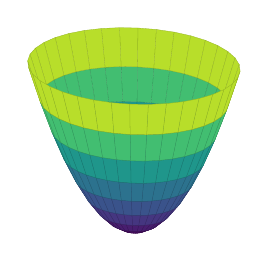
\begin{tikzpicture}
        \begin{axis}[width=5.6cm, height=5.6cm, view={35}{22}, axis lines=none, colormap/viridis, unit vector ratio=1 1 0.9]
            \addplot3[surf, shader=faceted, draw=black!40, line width=0.1pt, domain=0:2, y domain=0:360, samples=10, samples y=37, z buffer=sort] ({x*cos(y)}, {x*sin(y)}, {x^2});
        \end{axis}
    \end{tikzpicture}
    \hfill
    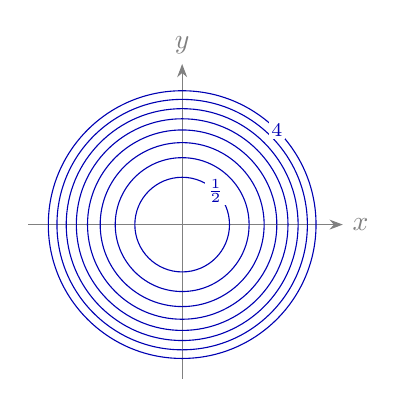
\begin{tikzpicture}[scale=0.85, >=Stealth]
        \draw[->, gray] (-2.3,0) -- (2.4,0) node[right] {$x$};
        \draw[->, gray] (0,-2.3) -- (0,2.4) node[above] {$y$};
        \foreach \k in {1,...,8}
            \draw[blue!70!black] (0,0) circle ({sqrt(0.5*\k)});
        \node[blue!70!black, font=\scriptsize, fill=white, inner sep=1pt] at (45:2) {$4$};
        \node[blue!70!black, font=\scriptsize, fill=white, inner sep=1pt] at (45:{sqrt(0.5)}) {$\tfrac{1}{2}$};
    \end{tikzpicture}
    \hfill
    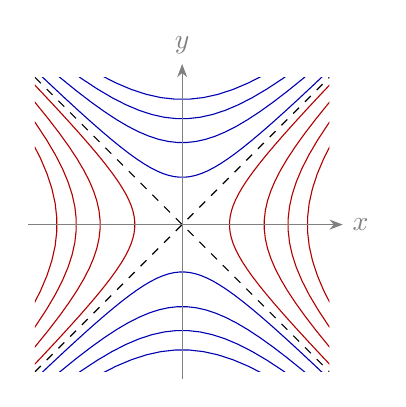
\begin{tikzpicture}[scale=0.85, >=Stealth]
        \begin{scope}
            \clip (-2.2,-2.2) rectangle (2.2,2.2);
            \foreach \c in {0.5,1.5,2.5,3.5} {
                \draw[red!70!black, domain=-2.2:2.2, samples=40, variable=\t] plot ({sqrt(\c)*cosh(\t)}, {sqrt(\c)*sinh(\t)});
                \draw[red!70!black, domain=-2.2:2.2, samples=40, variable=\t] plot ({-sqrt(\c)*cosh(\t)}, {sqrt(\c)*sinh(\t)});
                \draw[blue!70!black, domain=-2.2:2.2, samples=40, variable=\t] plot ({sqrt(\c)*sinh(\t)}, {sqrt(\c)*cosh(\t)});
                \draw[blue!70!black, domain=-2.2:2.2, samples=40, variable=\t] plot ({sqrt(\c)*sinh(\t)}, {-sqrt(\c)*cosh(\t)});
            }
            \draw[dashed] (-2.2,-2.2) -- (2.2,2.2);
            \draw[dashed] (-2.2,2.2) -- (2.2,-2.2);
        \end{scope}
        \draw[->, gray] (-2.3,0) -- (2.4,0) node[right] {$x$};
        \draw[->, gray] (0,-2.3) -- (0,2.4) node[above] {$y$};
    \end{tikzpicture}
    \caption{Left: the graph of $f(x, y) = x^2 + y^2$, a paraboloid. Middle: its level curves for the levels $c = \frac{1}{2}, 1, \frac{3}{2}, \ldots, 4$, which are circles of radius $\sqrt{c}$. They get closer together as we move away from the origin, because $f$ gets steeper. Right: level curves of $g(x, y) = x^2 - y^2$ for $c = \pm\frac{1}{2}, \pm\frac{3}{2}, \pm\frac{5}{2}, \pm\frac{7}{2}$ (red: $c > 0$, blue: $c < 0$), and the level set $c = 0$ (dashed).}
    \label{L3-fig:level-sets}
\end{figure}

\subsection{Limits and continuity}

\begin{definition}[Limits and continuity]\label{L3-def:limit}
    Let $f: D \to \mathbb{R}^m$ with $D \subseteq \mathbb{R}^n$, and let $\mathbf{a} \in \mathbb{R}^n$ be a point such that all points $\mathbf{x} \neq \mathbf{a}$ of some ball $B(\mathbf{a}, r)$ lie in $D$. We say that $f(\mathbf{x})$ converges to $\mathbf{L} \in \mathbb{R}^m$ as $\mathbf{x}$ tends to $\mathbf{a}$, and write $\lim_{\mathbf{x} \to \mathbf{a}} f(\mathbf{x}) = \mathbf{L}$, if for every $\varepsilon > 0$ there is a $\delta > 0$ such that
    \[\norm{f(\mathbf{x}) - \mathbf{L}} < \varepsilon \qquad \text{for all } \mathbf{x} \in D \text{ with } 0 < \norm{\mathbf{x} - \mathbf{a}} < \delta.\]
    If $\mathbf{a} \in D$, then $f$ is continuous at $\mathbf{a}$ if $\lim_{\mathbf{x} \to \mathbf{a}} f(\mathbf{x}) = f(\mathbf{a})$. The function $f$ is continuous if it is continuous at every point of $D$.
\end{definition}

By the inequalities $\norm{\mathbf{x}}_\infty \leq \norm{\mathbf{x}}_2 \leq \norm{\mathbf{x}}_1 \leq n \norm{\mathbf{x}}_\infty$ of Lecture~2, we could use the $\ell_1$ or the $\ell_\infty$ norm instead of the Euclidean norm in this definition, without changing its meaning. In particular, since
\[|f_i(\mathbf{x}) - L_i| \leq \norm{f(\mathbf{x}) - \mathbf{L}} \leq |f_1(\mathbf{x}) - L_1| + \cdots + |f_m(\mathbf{x}) - L_m|,\]
$f(\mathbf{x})$ converges to $\mathbf{L}$ if and only if every component $f_i(\mathbf{x})$ converges to $L_i$, and $f$ is continuous if and only if all its components are continuous.

As for functions of one variable, sums, products, quotients (where the denominator is not zero) and compositions of continuous functions are continuous, and the coordinate functions $\mathbf{x} \mapsto x_i$ are continuous, since $|x_i - a_i| \leq \norm{\mathbf{x} - \mathbf{a}}$. Hence polynomials in $x_1, \ldots, x_n$, linear maps $\mathbf{x} \mapsto A\mathbf{x}$, and functions such as $e^{x_1} \sin(x_2)$ or the functions of Example~\ref{L3-ex:ml-functions} are continuous.

\begin{example}\label{L3-ex:xy}
    Let $f(x, y) = \frac{xy}{x^2 + y^2}$ for $(x, y) \neq (0, 0)$, and $f(0, 0) = 0$. On the coordinate axes, $f$ is $0$. On the line $y = x$, we have $f(t, t) = \frac{t^2}{2t^2} = \frac{1}{2}$ for $t \neq 0$. So arbitrarily close to the origin, there are points where $f$ is $0$ and points where $f$ is $\frac{1}{2}$, and $f(\mathbf{x})$ has no limit as $\mathbf{x} \to \mathbf{0}$. In particular, $f$ is not continuous at the origin, although the functions $t \mapsto f(t, 0)$ and $t \mapsto f(0, t)$ are continuous (they are constant). More generally, $f$ is constant on every line through the origin: $f(t, mt) = \frac{m}{1 + m^2}$ for $t \neq 0$.
\end{example}

The lesson of this example is that to understand a function near a point, it is not enough to look at it along the coordinate axes. We will meet this function again when we discuss derivatives.

\section{Derivatives of Functions of One Variable}\label{L3-sec:univariate}

We first recall derivatives of functions $f: \mathbb{R} \to \mathbb{R}$, and rewrite the definition in a form that generalizes to several variables.

\begin{definition}[Derivative]\label{L3-def:derivative}
    Let $f: D \to \mathbb{R}$ with $D \subseteq \mathbb{R}$ open, and let $x \in D$. The function $f$ is differentiable at $x$ if the limit
    \[f'(x) = \lim_{h \to 0} \frac{f(x + h) - f(x)}{h}\]
    exists. Then $f'(x)$, also written $\frac{df}{dx}(x)$, is the derivative of $f$ at $x$. The function $f$ is differentiable if it is differentiable at every point of $D$.
\end{definition}

The quotient $\frac{f(x + h) - f(x)}{h}$ is the slope of the line through the points $(x, f(x))$ and $(x + h, f(x + h))$ of the graph, and its limit $f'(x)$ is the slope of the tangent line to the graph at $x$.

\begin{proposition}[Linear approximation]\label{L3-prop:linear-approx-1d}
    Let $c \in \mathbb{R}$. Then $f$ is differentiable at $x$ with $f'(x) = c$ if and only if
    \[f(x + h) = f(x) + c h + r(h), \qquad \text{where } \lim_{h \to 0} \frac{r(h)}{h} = 0.\]
\end{proposition}

\begin{proof}
    Let $r(h) = f(x + h) - f(x) - ch$. Then $\frac{r(h)}{h} = \frac{f(x + h) - f(x)}{h} - c$, which converges to $0$ if and only if the difference quotient converges to $c$.
\end{proof}

We write $r(h) = o(|h|)$, read ``little o of $|h|$'', if $\frac{r(h)}{|h|} \to 0$ as $h \to 0$: the error $r(h)$ is small even compared with the small number $|h|$. So $f$ is differentiable at $x$ if and only if near $x$, it is approximated by the affine function $h \mapsto f(x) + f'(x) h$, with an error that is $o(|h|)$. This description of the derivative, as the slope of the best linear approximation, is the one that generalizes to functions of several variables.

\begin{proposition}[Rules of differentiation]\label{L3-prop:rules-1d}
    Let $f$ and $g$ be differentiable at $x$, and let $\lambda \in \mathbb{R}$. Then:
    \begin{enumerate}
        \item $(f + g)'(x) = f'(x) + g'(x)$ and $(\lambda f)'(x) = \lambda f'(x)$;
        \item product rule: $(fg)'(x) = f'(x) g(x) + f(x) g'(x)$;
        \item quotient rule: if $g(x) \neq 0$, then $\big(\frac{f}{g}\big)'(x) = \frac{f'(x) g(x) - f(x) g'(x)}{g(x)^2}$;
        \item chain rule: if $\varphi$ is differentiable at $g(x)$, then $(\varphi \circ g)'(x) = \varphi'(g(x))\, g'(x)$.
    \end{enumerate}
\end{proposition}

We assume these rules from calculus, together with the derivatives of the standard functions: $(x^k)' = k x^{k-1}$, $(e^x)' = e^x$, $(\log x)' = \frac{1}{x}$ for $x > 0$, $\sin' = \cos$ and $\cos' = -\sin$. Part (1) says that differentiation is a linear map, as in Lecture~1.

\begin{example}[Activation functions]\label{L3-ex:sigmoid}
    The sigmoid function $\sigma(x) = \frac{1}{1 + e^{-x}}$ has the derivative
    \[\sigma'(x) = \frac{e^{-x}}{(1 + e^{-x})^2} = \sigma(x) \big(1 - \sigma(x)\big),\]
    since $1 - \sigma(x) = \frac{e^{-x}}{1 + e^{-x}}$. So the derivative can be computed from the value $\sigma(x)$, which saves work when training neural networks. Since $t(1 - t) \leq \frac{1}{4}$ for all $t$, we have $0 < \sigma'(x) \leq \frac{1}{4}$, with the maximum at $x = 0$. Similarly, $\tanh'(x) = 1 - \tanh(x)^2$. The ReLU function has derivative $0$ for $x < 0$ and $1$ for $x > 0$, but it is not differentiable at $0$: the difference quotient $\frac{\ReLU(h) - \ReLU(0)}{h}$ is $1$ for $h > 0$ and $0$ for $h < 0$. In practice, software simply uses the derivative $0$ at $x = 0$; since an input is very rarely exactly $0$, this causes no problems.
\end{example}

If $f'$ is differentiable, its derivative is the second derivative $f''$, and similarly we define the $k$-th derivative $f^{(k)}$. A function is $k$ times continuously differentiable if $f^{(k)}$ exists and is continuous.

\subsection{Taylor polynomials}

The linear approximation of $f$ near $x_0$ only uses $f(x_0)$ and $f'(x_0)$. Using higher derivatives, we get better approximations by polynomials.

\begin{definition}[Taylor polynomial]\label{L3-def:taylor-polynomial}
    Let $f$ be $k$ times differentiable at $x_0$. The Taylor polynomial of degree $k$ of $f$ at $x_0$ is
    \begin{align*}
        T_k(x) &= \sum_{j=0}^k \frac{f^{(j)}(x_0)}{j!} (x - x_0)^j \\
        &= f(x_0) + f'(x_0)(x - x_0) + \frac{f''(x_0)}{2}(x - x_0)^2 + \cdots + \frac{f^{(k)}(x_0)}{k!}(x - x_0)^k.
    \end{align*}
\end{definition}

The coefficients are chosen such that $T_k$ and $f$ have the same derivatives of orders $0, 1, \ldots, k$ at $x_0$: the $j$-th derivative of $\frac{(x - x_0)^i}{i!}$ at $x_0$ is $1$ if $i = j$, and $0$ otherwise. The Taylor polynomial $T_1(x) = f(x_0) + f'(x_0)(x - x_0)$ is the tangent line.

\begin{theorem}[Taylor's theorem]\label{L3-thm:taylor-1d}
    Let $f$ be $k + 1$ times differentiable on an open interval $I$ that contains $x_0$ and $x$. Then there is a number $\xi$ between $x_0$ and $x$ such that
    \[f(x) = T_k(x) + \frac{f^{(k+1)}(\xi)}{(k+1)!} (x - x_0)^{k+1}.\]
\end{theorem}

For $k = 0$, this is the mean value theorem $f(x) - f(x_0) = f'(\xi)(x - x_0)$. We do not prove the theorem here. It says that if $|f^{(k+1)}| \leq M$ on $I$, then the error of the approximation $f(x) \approx T_k(x)$ is at most $\frac{M}{(k+1)!}|x - x_0|^{k+1}$, which is tiny when $x$ is close to $x_0$.

\begin{example}\label{L3-ex:taylor-exp}
    All derivatives of $e^x$ are $e^x$, so its Taylor polynomials at $x_0 = 0$ are $T_k(x) = 1 + x + \frac{x^2}{2!} + \cdots + \frac{x^k}{k!}$. For example, $e^{0.1} \approx T_2(0.1) = 1 + 0.1 + 0.005 = 1.105$. By Taylor's theorem, the error is $\frac{e^\xi}{3!} (0.1)^3$ for some $0 < \xi < 0.1$, which is at most $\frac{e^{0.1}}{6000} < 0.0002$. Indeed, $e^{0.1} = 1.10517\ldots$.
\end{example}

\begin{example}\label{L3-ex:taylor-cos}
    The derivatives of $\cos$ at $0$ are $1, 0, -1, 0, 1, 0, -1, 0, \ldots$, so the Taylor polynomials of $\cos$ at $0$ are
    \[T_{2k}(x) = 1 - \frac{x^2}{2!} + \frac{x^4}{4!} - \cdots + (-1)^k \frac{x^{2k}}{(2k)!}.\]
    Figure~\ref{L3-fig:taylor-cos} shows that they approximate $\cos$ on larger and larger intervals. Since all derivatives of $\cos$ are bounded by $1$, Taylor's theorem gives $|\cos x - T_k(x)| \leq \frac{|x|^{k+1}}{(k+1)!}$, which tends to $0$ as $k \to \infty$ for every fixed $x$, since factorials grow faster than powers. Hence $\cos x = \sum_{j=0}^\infty (-1)^j \frac{x^{2j}}{(2j)!}$ for all $x \in \mathbb{R}$: the Taylor series of $\cos$ converges to $\cos$ everywhere. Not all functions behave this nicely. For example, the Taylor series $x - \frac{x^2}{2} + \frac{x^3}{3} - \cdots$ of $\log(1 + x)$ at $0$ only converges for $-1 < x \leq 1$.
\end{example}

\begin{figure}[ht]
    \centering
    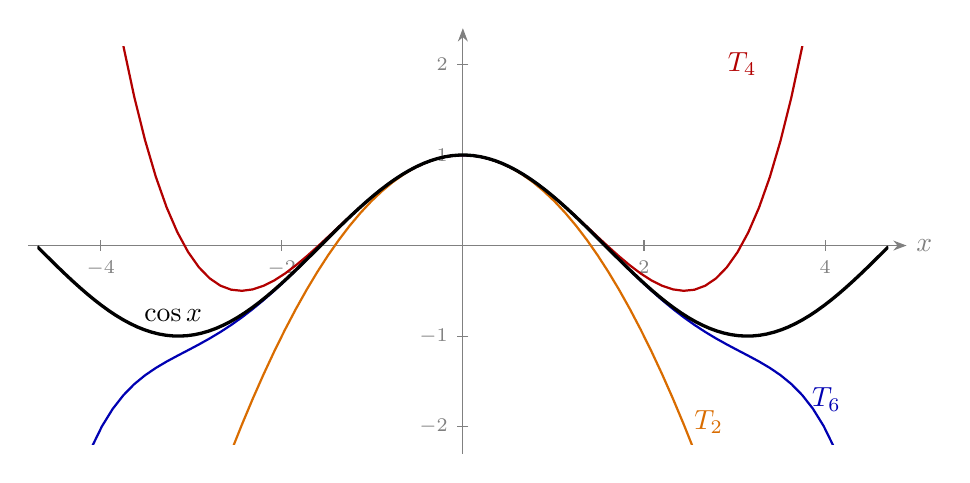
\begin{tikzpicture}[x=1.15cm, y=1.15cm, >=Stealth]
        \draw[->, gray] (-4.8,0) -- (4.9,0) node[right] {$x$};
        \draw[->, gray] (0,-2.3) -- (0,2.4);
        \foreach \t in {-4,-2,2,4}
            \draw[gray] (\t,0.06) -- (\t,-0.06) node[below, font=\scriptsize] {$\t$};
        \foreach \t in {-2,-1,1,2}
            \draw[gray] (0.06,\t) -- (-0.06,\t) node[left, font=\scriptsize] {$\t$};
        \begin{scope}
            \clip (-4.7,-2.2) rectangle (4.7,2.2);
            \draw[orange!85!black, thick, domain=-4.7:4.7, samples=80] plot (\x, {1 - (\x)^2/2});
            \draw[red!70!black, thick, domain=-4.7:4.7, samples=80] plot (\x, {1 - (\x)^2/2 + (\x)^4/24});
            \draw[blue!70!black, thick, domain=-4.7:4.7, samples=80] plot (\x, {1 - (\x)^2/2 + (\x)^4/24 - (\x)^6/720});
            \draw[black, very thick, domain=-4.7:4.7, samples=120] plot (\x, {cos(\x r)});
        \end{scope}
        \node[orange!85!black, right] at (2.45,-1.95) {$T_2$};
        \node[red!70!black, left] at (3.35,2.0) {$T_4$};
        \node[blue!70!black, right] at (3.75,-1.7) {$T_6$};
        \node[black, above] at (-3.2,-0.95) {$\cos x$};
    \end{tikzpicture}
    \caption{The function $\cos x$ (black) and its Taylor polynomials $T_2$, $T_4$ and $T_6$ at $0$. Near $0$, all of them are good approximations, and higher degrees give good approximations on larger intervals.}
    \label{L3-fig:taylor-cos}
\end{figure}

Taylor's theorem also tells us how to compute derivatives numerically, and how accurate the result is.

\begin{proposition}[Finite differences]\label{L3-prop:finite-differences}
    Let $h > 0$, and let $f$ be three times differentiable on an open interval containing $[x - h, x + h]$, with $|f''| \leq M_2$ and $|f'''| \leq M_3$ there. Then
    \[\left| \frac{f(x + h) - f(x)}{h} - f'(x) \right| \leq \frac{M_2}{2} h \qquad \text{and} \qquad \left| \frac{f(x + h) - f(x - h)}{2h} - f'(x) \right| \leq \frac{M_3}{6} h^2.\]
\end{proposition}

\begin{proof}
    By Taylor's theorem with $k = 1$, $f(x + h) = f(x) + f'(x) h + \frac{f''(\xi)}{2} h^2$, so the error of the forward difference is $\frac{f''(\xi)}{2} h$. With $k = 2$,
    \[f(x \pm h) = f(x) \pm f'(x) h + \frac{f''(x)}{2} h^2 \pm \frac{f'''(\xi_\pm)}{6} h^3\]
    for some $\xi_+$ and $\xi_-$. Subtracting the two equations gives $f(x + h) - f(x - h) = 2 f'(x) h + \frac{f'''(\xi_+) + f'''(\xi_-)}{6} h^3$. We divide by $2h$; the error is $\frac{f'''(\xi_+) + f'''(\xi_-)}{12} h^2$, which is at most $\frac{M_3}{6} h^2$.
\end{proof}

The central difference $\frac{f(x + h) - f(x - h)}{2h}$ is much more accurate than the forward difference: halving $h$ divides its error by $4$ instead of $2$. In machine learning, it is used for gradient checking, i.e., to test a program that computes derivatives. The step $h$ cannot be chosen arbitrarily small, though: computers store numbers with about $16$ significant digits, and in the difference $f(x + h) - f(x - h)$ of two almost equal numbers, most of these digits cancel (see Programming Exercise~P1).

\section{Partial Derivatives and Gradients}\label{L3-sec:gradients}

For a function of several variables, the simplest way to take a derivative is to vary only one variable and to keep all others fixed.

\begin{definition}[Partial derivatives and gradient]\label{L3-def:partial}
    Let $f: D \to \mathbb{R}$ with $D \subseteq \mathbb{R}^n$ open, and let $\mathbf{x} \in D$. The partial derivative of $f$ with respect to $x_i$ at $\mathbf{x}$ is
    \[\frac{\partial f}{\partial x_i}(\mathbf{x}) = \lim_{h \to 0} \frac{f(\mathbf{x} + h\mathbf{e}_i) - f(\mathbf{x})}{h},\]
    if this limit exists. If all partial derivatives of $f$ at $\mathbf{x}$ exist, the gradient of $f$ at $\mathbf{x}$ is the column vector
    \[\nabla f(\mathbf{x}) = \begin{pmatrix} \frac{\partial f}{\partial x_1}(\mathbf{x}) \\ \vdots \\ \frac{\partial f}{\partial x_n}(\mathbf{x}) \end{pmatrix} \in \mathbb{R}^n.\]
\end{definition}

The partial derivative $\frac{\partial f}{\partial x_i}(\mathbf{x})$ is the ordinary derivative at $t = x_i$ of the function of one variable
\[t \mapsto f(x_1, \ldots, x_{i-1}, t, x_{i+1}, \ldots, x_n).\]
So we compute it with the rules of Section~\ref{L3-sec:univariate}, treating all variables other than $x_i$ as constants.

\begin{example}\label{L3-ex:partials}
    Let $f(x_1, x_2) = x_1^2 x_2 + x_1 x_2^3$. Treating $x_2$ as a constant, and then $x_1$ as a constant, we get
    \[\frac{\partial f}{\partial x_1} = 2x_1 x_2 + x_2^3, \qquad \frac{\partial f}{\partial x_2} = x_1^2 + 3x_1 x_2^2.\]
    At $\mathbf{x} = (1, 2)^\top$, the gradient is $\nabla f(\mathbf{x}) = (4 + 8, \, 1 + 12)^\top = (12, 13)^\top$.
\end{example}

\begin{proposition}\label{L3-prop:basic-gradients}
    Let $\mathbf{a} \in \mathbb{R}^n$ and $A \in \mathbb{R}^{n \times n}$. Then for all $\mathbf{x} \in \mathbb{R}^n$:
    \begin{enumerate}
        \item $\nabla (\mathbf{a}^\top \mathbf{x}) = \mathbf{a}$;
        \item $\nabla (\mathbf{x}^\top A \mathbf{x}) = (A + A^\top)\mathbf{x}$; in particular, $\nabla (\mathbf{x}^\top A \mathbf{x}) = 2A\mathbf{x}$ if $A$ is symmetric, and $\nabla \norm{\mathbf{x}}^2 = 2\mathbf{x}$;
        \item $\nabla \norm{\mathbf{x}} = \frac{\mathbf{x}}{\norm{\mathbf{x}}}$ for $\mathbf{x} \neq \mathbf{0}$.
    \end{enumerate}
\end{proposition}

\begin{proof}
    (1) Since $\mathbf{a}^\top \mathbf{x} = \sum_j a_j x_j$, the partial derivative with respect to $x_k$ is $a_k$.

    (2) We have $\mathbf{x}^\top A \mathbf{x} = \sum_{i, j} A_{ij} x_i x_j$. The terms that contain $x_k$ are those with $i = k$ or $j = k$, and differentiating them gives
    \[\frac{\partial}{\partial x_k} \mathbf{x}^\top A \mathbf{x} = \sum_j A_{kj} x_j + \sum_i A_{ik} x_i = (A\mathbf{x})_k + (A^\top \mathbf{x})_k.\]
    (The term $A_{kk} x_k^2$ has the derivative $2A_{kk} x_k$, which is counted once in each sum.) For $A = I_n$, we get $\nabla \norm{\mathbf{x}}^2 = \nabla(\mathbf{x}^\top \mathbf{x}) = 2\mathbf{x}$.

    (3) By the chain rule, $\frac{\partial}{\partial x_k} \big(x_1^2 + \cdots + x_n^2\big)^{1/2} = \frac{1}{2} \big(x_1^2 + \cdots + x_n^2\big)^{-1/2} \cdot 2x_k = \frac{x_k}{\norm{\mathbf{x}}}$.
\end{proof}

These formulas look like their one-variable versions $(ax)' = a$ and $(ax^2)' = 2ax$, and they will be used constantly. Note that the gradient of the Euclidean norm is a unit vector, which points away from the origin.

\subsection{Differentiability}

Partial derivatives only describe $f$ along the coordinate axes, and by Example~\ref{L3-ex:xy}, this is not enough. The function $f(x, y) = \frac{xy}{x^2 + y^2}$ of that example is $0$ on both axes, so both partial derivatives at the origin exist and are $0$. But $f$ is not even continuous at the origin, so it would be strange to call it differentiable there. The right definition generalizes Proposition~\ref{L3-prop:linear-approx-1d}: $f$ should be approximated by a linear function near $\mathbf{x}$, in all directions at once. As before, we write $r(\mathbf{h}) = o(\norm{\mathbf{h}})$ if $\frac{r(\mathbf{h})}{\norm{\mathbf{h}}} \to 0$ as $\mathbf{h} \to \mathbf{0}$.

\begin{definition}[Differentiable function]\label{L3-def:differentiable}
    Let $f: D \to \mathbb{R}$ with $D \subseteq \mathbb{R}^n$ open, and let $\mathbf{x} \in D$. The function $f$ is differentiable at $\mathbf{x}$ if there is a row vector $\mathbf{c} \in \mathbb{R}^{1 \times n}$ such that
    \[f(\mathbf{x} + \mathbf{h}) = f(\mathbf{x}) + \mathbf{c}\mathbf{h} + r(\mathbf{h}), \qquad \text{where } r(\mathbf{h}) = o(\norm{\mathbf{h}}).\]
    The row vector $\mathbf{c}$, or the linear map $\mathbf{h} \mapsto \mathbf{c}\mathbf{h}$, is then called the derivative of $f$ at $\mathbf{x}$, and is denoted by $Df(\mathbf{x})$. The function $f$ is differentiable if it is differentiable at every point of $D$.
\end{definition}

\begin{proposition}\label{L3-prop:differentiable}
    Let $f$ be differentiable at $\mathbf{x}$, with derivative $Df(\mathbf{x}) = \mathbf{c}$. Then:
    \begin{enumerate}
        \item for every vector $\mathbf{v} \in \mathbb{R}^n$, the directional derivative of $f$ at $\mathbf{x}$ in the direction $\mathbf{v}$,
        \[D_{\mathbf{v}} f(\mathbf{x}) = \lim_{t \to 0} \frac{f(\mathbf{x} + t\mathbf{v}) - f(\mathbf{x})}{t},\]
        exists and is equal to $\mathbf{c}\mathbf{v}$;
        \item all partial derivatives of $f$ at $\mathbf{x}$ exist, and $\mathbf{c} = \big(\frac{\partial f}{\partial x_1}(\mathbf{x}), \ldots, \frac{\partial f}{\partial x_n}(\mathbf{x})\big)$. In other words, $Df(\mathbf{x}) = \nabla f(\mathbf{x})^\top$, and $D_{\mathbf{v}} f(\mathbf{x}) = \nabla f(\mathbf{x})^\top \mathbf{v}$;
        \item $f$ is continuous at $\mathbf{x}$.
    \end{enumerate}
\end{proposition}

\begin{proof}
    (1) For $\mathbf{v} = \mathbf{0}$, both sides are $0$. For $\mathbf{v} \neq \mathbf{0}$ and $t \neq 0$, we apply the definition with $\mathbf{h} = t\mathbf{v}$:
    \[\left| \frac{f(\mathbf{x} + t\mathbf{v}) - f(\mathbf{x})}{t} - \mathbf{c}\mathbf{v} \right| = \frac{|r(t\mathbf{v})|}{|t|} = \norm{\mathbf{v}} \frac{|r(t\mathbf{v})|}{\norm{t\mathbf{v}}},\]
    which tends to $0$ as $t \to 0$.

    (2) The partial derivative $\frac{\partial f}{\partial x_i}(\mathbf{x})$ is the directional derivative in the direction $\mathbf{e}_i$, which by (1) is $\mathbf{c}\mathbf{e}_i = c_i$.

    (3) We have $|f(\mathbf{x} + \mathbf{h}) - f(\mathbf{x})| \leq |\mathbf{c}\mathbf{h}| + |r(\mathbf{h})| \leq \norm{\mathbf{c}} \norm{\mathbf{h}} + |r(\mathbf{h})|$ by the Cauchy--Schwarz inequality, and both terms tend to $0$ as $\mathbf{h} \to \mathbf{0}$.
\end{proof}

By (3), the function of Example~\ref{L3-ex:xy} is not differentiable at the origin, although its partial derivatives exist there. So differentiability is a stronger condition than the existence of partial derivatives. Fortunately, the following theorem, which we do not prove, shows that almost all functions that we meet in practice are differentiable.

\begin{theorem}\label{L3-thm:C1}
    Let $f: D \to \mathbb{R}$ with $D \subseteq \mathbb{R}^n$ open. If all partial derivatives of $f$ exist in a ball around $\mathbf{x}$ and are continuous at $\mathbf{x}$, then $f$ is differentiable at $\mathbf{x}$.
\end{theorem}

A function whose partial derivatives exist and are continuous on $D$ is called continuously differentiable. By Theorem~\ref{L3-thm:C1}, polynomials, and functions built from $\exp$, $\log$, $\sin$, the sigmoid function, etc., by sums, products, quotients and compositions, are differentiable wherever they are defined. Some important functions in machine learning are differentiable only at most points, such as $\ReLU$, the $\ell_1$ norm, and the hinge loss $\max(0, 1 - t)$; at the few points where they are not differentiable, software uses a reasonable substitute for the derivative.

\begin{remark}[Notation]
    In this lecture, as in the remark on gradients in the section on dual spaces in Lecture~1, the derivative $Df(\mathbf{x})$ of a function $f: \mathbb{R}^n \to \mathbb{R}$ is a row vector, and the gradient $\nabla f(\mathbf{x}) = Df(\mathbf{x})^\top$ is a column vector. Some books call the row vector the gradient. In machine learning software such as PyTorch, the gradient with respect to a parameter always has the same shape as the parameter, so it is a column vector for a vector of parameters, and a matrix for a matrix of parameters (Section~\ref{L3-sec:matrix-gradients}).
\end{remark}

\begin{remark}[The gradient depends on the inner product]\label{L3-rem:riesz}
    The derivative $Df(\mathbf{x})$ is a linear functional $\mathbb{R}^n \to \mathbb{R}$, i.e., an element of the dual space $(\mathbb{R}^n)^*$ of Lecture~1. The gradient is the vector that represents this linear functional with respect to the dot product:
    \[Df(\mathbf{x})\mathbf{h} = \ip{\nabla f(\mathbf{x})}{\mathbf{h}} \qquad \text{for all } \mathbf{h} \in \mathbb{R}^n.\]
    In every finite-dimensional inner product space, every linear functional is represented in this way by a unique vector; this is the Riesz representation theorem. If we use a different inner product on $\mathbb{R}^n$, such as $\ip{\mathbf{x}}{\mathbf{y}}_A = \mathbf{x}^\top A \mathbf{y}$ for a symmetric positive definite matrix $A$ (Lecture~2), then the vector that represents $Df(\mathbf{x})$ changes: since
    \[\ip{A^{-1} \nabla f(\mathbf{x})}{\mathbf{h}}_A = \nabla f(\mathbf{x})^\top A^{-1} A \mathbf{h} = Df(\mathbf{x})\mathbf{h},\]
    the gradient with respect to $\ip{\cdot}{\cdot}_A$ is $A^{-1} \nabla f(\mathbf{x})$. So the derivative is determined by $f$ alone, but the gradient also depends on how we measure lengths and angles. Changing the inner product is the idea behind preconditioning and the natural gradient method, and Newton's method in Section~\ref{L3-sec:newton} is an example.
\end{remark}

\subsection{Directional derivatives and steepest ascent}

By Proposition~\ref{L3-prop:differentiable}, the rate of change of a differentiable function in the direction $\mathbf{v}$ is $D_{\mathbf{v}} f(\mathbf{x}) = \nabla f(\mathbf{x})^\top \mathbf{v}$. In which direction does $f$ increase fastest?

\begin{theorem}[Steepest ascent]\label{L3-thm:steepest}
    Let $f$ be differentiable at $\mathbf{x}$, with $\nabla f(\mathbf{x}) \neq \mathbf{0}$. Then for every unit vector $\mathbf{v}$,
    \[-\norm{\nabla f(\mathbf{x})} \leq D_{\mathbf{v}} f(\mathbf{x}) \leq \norm{\nabla f(\mathbf{x})}.\]
    The maximum is attained only for $\mathbf{v} = \frac{\nabla f(\mathbf{x})}{\norm{\nabla f(\mathbf{x})}}$, and the minimum only for $\mathbf{v} = -\frac{\nabla f(\mathbf{x})}{\norm{\nabla f(\mathbf{x})}}$.
\end{theorem}

\begin{proof}
    By the Cauchy--Schwarz inequality (Lecture~2), $|D_{\mathbf{v}} f(\mathbf{x})| = |\nabla f(\mathbf{x})^\top \mathbf{v}| \leq \norm{\nabla f(\mathbf{x})} \norm{\mathbf{v}} = \norm{\nabla f(\mathbf{x})}$, with equality if and only if $\mathbf{v}$ is a multiple of $\nabla f(\mathbf{x})$. The only unit vectors that are multiples of $\nabla f(\mathbf{x})$ are $\pm \frac{\nabla f(\mathbf{x})}{\norm{\nabla f(\mathbf{x})}}$, and they give $D_{\mathbf{v}} f(\mathbf{x}) = \pm \norm{\nabla f(\mathbf{x})}$.
\end{proof}

So the gradient points in the direction in which $f$ increases fastest, and its length is the rate of increase in this direction. The negative gradient $-\nabla f(\mathbf{x})$ is the direction of steepest descent, which is the direction that gradient descent uses to decrease a loss function (Section~\ref{L3-sec:gd}). In directions orthogonal to $\nabla f(\mathbf{x})$, the rate of change is $0$; we will see in Section~\ref{L3-sec:chain-rule} that these are the directions tangent to the level set through $\mathbf{x}$.

\begin{example}\label{L3-ex:directional}
    For the function $f(x_1, x_2) = x_1^2 x_2 + x_1 x_2^3$ of Example~\ref{L3-ex:partials}, at $\mathbf{x} = (1, 2)^\top$, we found $\nabla f(\mathbf{x}) = (12, 13)^\top$. In the direction of the unit vector $\mathbf{v} = \frac{1}{5}(3, 4)^\top$, the rate of change is $D_{\mathbf{v}} f(\mathbf{x}) = \frac{1}{5}(36 + 52) = 17.6$. The largest possible rate is $\norm{\nabla f(\mathbf{x})} = \sqrt{313} \approx 17.69$, in the direction $\frac{1}{\sqrt{313}}(12, 13)^\top$, and in the orthogonal direction $\frac{1}{\sqrt{313}}(13, -12)^\top$ the rate of change is $0$.
\end{example}

\section{Jacobians: Derivatives of Vector-Valued Functions}\label{L3-sec:jacobians}

Many functions in machine learning have vector outputs, such as the layers of a neural network. Their derivatives are matrices.

\begin{definition}[Jacobian]\label{L3-def:jacobian}
    Let $f: D \to \mathbb{R}^m$ with $D \subseteq \mathbb{R}^n$ open, and let $\mathbf{x} \in D$. The function $f$ is differentiable at $\mathbf{x}$ if there is an $m \times n$ matrix $J$ such that
    \[f(\mathbf{x} + \mathbf{h}) = f(\mathbf{x}) + J\mathbf{h} + \mathbf{r}(\mathbf{h}), \qquad \text{where } \lim_{\mathbf{h} \to \mathbf{0}} \frac{\norm{\mathbf{r}(\mathbf{h})}}{\norm{\mathbf{h}}} = 0.\]
    The matrix $J$ is called the Jacobian matrix, or the derivative, of $f$ at $\mathbf{x}$, and is denoted by $Df(\mathbf{x})$ or $J_f(\mathbf{x})$.
\end{definition}

For $m = 1$, this is Definition~\ref{L3-def:differentiable}. The next proposition shows that the Jacobian consists of the derivatives of the components of $f$.

\begin{proposition}\label{L3-prop:jacobian-entries}
    A function $f = (f_1, \ldots, f_m)^\top$ is differentiable at $\mathbf{x}$ if and only if all its components $f_i$ are differentiable at $\mathbf{x}$. In this case, the $i$-th row of $Df(\mathbf{x})$ is $Df_i(\mathbf{x}) = \nabla f_i(\mathbf{x})^\top$, i.e.,
    \[Df(\mathbf{x}) = \begin{pmatrix} \frac{\partial f_1}{\partial x_1}(\mathbf{x}) & \cdots & \frac{\partial f_1}{\partial x_n}(\mathbf{x}) \\ \vdots & & \vdots \\ \frac{\partial f_m}{\partial x_1}(\mathbf{x}) & \cdots & \frac{\partial f_m}{\partial x_n}(\mathbf{x}) \end{pmatrix}, \qquad \text{that is,} \quad \big(Df(\mathbf{x})\big)_{ij} = \frac{\partial f_i}{\partial x_j}(\mathbf{x}).\]
\end{proposition}

\begin{proof}
    The $i$-th component of the equation in Definition~\ref{L3-def:jacobian} is $f_i(\mathbf{x} + \mathbf{h}) = f_i(\mathbf{x}) + J_i\mathbf{h} + r_i(\mathbf{h})$, where $J_i$ is the $i$-th row of $J$. Since $|r_i(\mathbf{h})| \leq \norm{\mathbf{r}(\mathbf{h})} \leq |r_1(\mathbf{h})| + \cdots + |r_m(\mathbf{h})|$, we have $\frac{\norm{\mathbf{r}(\mathbf{h})}}{\norm{\mathbf{h}}} \to 0$ if and only if $\frac{r_i(\mathbf{h})}{\norm{\mathbf{h}}} \to 0$ for all $i$. So $f$ is differentiable with Jacobian $J$ if and only if every $f_i$ is differentiable with derivative $J_i$, and by Proposition~\ref{L3-prop:differentiable}, $J_i = \nabla f_i(\mathbf{x})^\top$.
\end{proof}

So the rows of the Jacobian correspond to the outputs of $f$, and the columns to the inputs: the $j$-th column $\frac{\partial f}{\partial x_j}(\mathbf{x})$ describes how the output vector changes when we change $x_j$. In the language of Lecture~1, the derivative of $f$ at $\mathbf{x}$ is the linear transformation $\mathbf{h} \mapsto Df(\mathbf{x})\mathbf{h}$ from $\mathbb{R}^n$ to $\mathbb{R}^m$ that best approximates the change $f(\mathbf{x} + \mathbf{h}) - f(\mathbf{x})$, and the Jacobian is its matrix with respect to the standard bases. Near $\mathbf{x}$,
\[f(\mathbf{x} + \mathbf{h}) \approx f(\mathbf{x}) + Df(\mathbf{x})\mathbf{h}:\]
a differentiable function looks like an affine function if we zoom in far enough.

\begin{example}\label{L3-ex:jacobian}
    Let $f(x_1, x_2) = (x_1^2 x_2, \, 3x_1 + x_2^2)^\top$. Then
    \[Df(\mathbf{x}) = \begin{pmatrix} 2x_1 x_2 & x_1^2 \\ 3 & 2x_2 \end{pmatrix}, \qquad \text{and at } \mathbf{a} = \begin{pmatrix} 1 \\ 2 \end{pmatrix}: \quad f(\mathbf{a}) = \begin{pmatrix} 2 \\ 7 \end{pmatrix}, \quad Df(\mathbf{a}) = \begin{pmatrix} 4 & 1 \\ 3 & 4 \end{pmatrix}.\]
    The linear approximation gives $f(1.1, 1.9) \approx f(\mathbf{a}) + Df(\mathbf{a}) \begin{pmatrix} 0.1 \\ -0.1 \end{pmatrix} = \begin{pmatrix} 2.3 \\ 6.9 \end{pmatrix}$, while the exact value is $(2.299, \, 6.91)^\top$.
\end{example}

\begin{example}[Affine maps]\label{L3-ex:affine-jacobian}
    Let $f(\mathbf{x}) = A\mathbf{x} + \mathbf{b}$ with $A \in \mathbb{R}^{m \times n}$ and $\mathbf{b} \in \mathbb{R}^m$. Then $f(\mathbf{x} + \mathbf{h}) = f(\mathbf{x}) + A\mathbf{h}$ exactly, so $Df(\mathbf{x}) = A$ for every $\mathbf{x}$: the best linear approximation of an affine map is its linear part. For $m = 1$ and $f(\mathbf{x}) = \mathbf{a}^\top \mathbf{x}$, this is Proposition~\ref{L3-prop:basic-gradients}(1) again.
\end{example}

\begin{example}[Functions applied entrywise]\label{L3-ex:entrywise}
    Let $\varphi: \mathbb{R} \to \mathbb{R}$ be differentiable, such as an activation function, and let $f: \mathbb{R}^n \to \mathbb{R}^n$ apply $\varphi$ to each entry, $f(\mathbf{x}) = (\varphi(x_1), \ldots, \varphi(x_n))^\top$. Since $f_i$ only depends on $x_i$, we have $\frac{\partial f_i}{\partial x_j} = 0$ for $i \neq j$, so
    \[Df(\mathbf{x}) = \diag\big(\varphi'(x_1), \ldots, \varphi'(x_n)\big).\]
    Multiplying a vector by a diagonal matrix multiplies its entries: $Df(\mathbf{x})\mathbf{v} = \varphi'(\mathbf{x}) \odot \mathbf{v}$, where $\varphi'(\mathbf{x}) = (\varphi'(x_1), \ldots, \varphi'(x_n))^\top$, and $\odot$ is the entrywise product (or Hadamard product) $(\mathbf{a} \odot \mathbf{b})_i = a_i b_i$. Computing the product in this way costs $n$ multiplications instead of $n^2$.
\end{example}

\begin{example}[Softmax]\label{L3-ex:softmax-jacobian}
    Let $\mathbf{s} = \softmax(\mathbf{z})$ with $\mathbf{z} \in \mathbb{R}^K$, i.e., $s_i = \frac{e^{z_i}}{S}$ with $S = e^{z_1} + \cdots + e^{z_K}$. Since $\frac{\partial S}{\partial z_j} = e^{z_j}$, the quotient rule gives
    \[\frac{\partial s_i}{\partial z_j} = \frac{\delta_{ij} e^{z_i} S - e^{z_i} e^{z_j}}{S^2} = s_i \delta_{ij} - s_i s_j, \qquad \text{where } \delta_{ij} = \begin{cases} 1 & \text{if } i = j, \\ 0 & \text{if } i \neq j. \end{cases}\]
    So $D\softmax(\mathbf{z}) = \diag(\mathbf{s}) - \mathbf{s}\mathbf{s}^\top$. For example, for $\mathbf{z} = (2, 1, 0)^\top$, we have $\mathbf{s} \approx (0.665, 0.245, 0.090)^\top$ and
    \[D\softmax(\mathbf{z}) \approx \begin{pmatrix} 0.223 & -0.163 & -0.060 \\ -0.163 & 0.185 & -0.022 \\ -0.060 & -0.022 & 0.082 \end{pmatrix}.\]
    The Jacobian is symmetric, and its rows sum to $0$: with $\mathbf{1} = (1, \ldots, 1)^\top$, we have $D\softmax(\mathbf{z})\mathbf{1} = \mathbf{s} - \mathbf{s}(\mathbf{s}^\top \mathbf{1}) = \mathbf{0}$, since the entries of $\mathbf{s}$ sum to $1$. This reflects a fact from the section on quotient spaces in Lecture~1: $\softmax(\mathbf{z} + c\mathbf{1}) = \softmax(\mathbf{z})$ for all $c \in \mathbb{R}$, so moving $\mathbf{z}$ in the direction $\mathbf{1}$ does not change the output, and $\mathbf{1}$ lies in the null space of the Jacobian.
\end{example}

\subsection{The Jacobian determinant}

If $m = n$, the Jacobian is a square matrix, and its determinant describes how $f$ changes areas and volumes near a point. By Lecture~1, the linear map $\mathbf{h} \mapsto A\mathbf{h}$ multiplies areas (for $n = 2$) and volumes (for $n \geq 3$) by $|\det A|$. Near $\mathbf{x}$, $f$ is approximately the affine map $\mathbf{h} \mapsto f(\mathbf{x}) + Df(\mathbf{x})\mathbf{h}$. So a small square with side length $\varepsilon$ at $\mathbf{x}$ is mapped approximately to the parallelogram spanned by $\varepsilon Df(\mathbf{x})\mathbf{e}_1$ and $\varepsilon Df(\mathbf{x})\mathbf{e}_2$, whose area is $|\det Df(\mathbf{x})| \, \varepsilon^2$: the number $|\det Df(\mathbf{x})|$ is the factor by which $f$ scales small areas near $\mathbf{x}$.

\begin{example}[Polar coordinates]\label{L3-ex:polar}
    The map $f(r, \varphi) = (r\cos\varphi, \, r\sin\varphi)^\top$ turns polar coordinates into Cartesian coordinates. Its Jacobian and Jacobian determinant are
    \[Df(r, \varphi) = \begin{pmatrix} \cos\varphi & -r\sin\varphi \\ \sin\varphi & r\cos\varphi \end{pmatrix}, \qquad \det Df(r, \varphi) = r\cos^2\varphi + r\sin^2\varphi = r.\]
    A small rectangle $[r, r + \Delta r] \times [\varphi, \varphi + \Delta\varphi]$ is mapped to a piece of an annulus, which is approximately a rectangle with sides $\Delta r$ and $r\Delta\varphi$ (an arc of a circle of radius $r$), with area approximately $r \, \Delta r \, \Delta\varphi$; see Figure~\ref{L3-fig:polar}. This explains the factor $r$ in the substitution rule for integrals in polar coordinates,
    \[\iint_{\mathbb{R}^2} g(x, y) \, dx \, dy = \int_0^{2\pi} \int_0^\infty g(r\cos\varphi, r\sin\varphi) \, r \, dr \, d\varphi.\]
    A famous application is the Gaussian integral. Since $e^{-(x^2 + y^2)} = e^{-x^2} e^{-y^2}$,
    \[\left(\int_{-\infty}^\infty e^{-x^2} dx\right)^2 = \iint_{\mathbb{R}^2} e^{-(x^2 + y^2)} \, dx \, dy = \int_0^{2\pi} \int_0^\infty e^{-r^2} r \, dr \, d\varphi = 2\pi \left[-\tfrac{1}{2} e^{-r^2}\right]_0^\infty = \pi,\]
    so $\int_{-\infty}^\infty e^{-x^2} dx = \sqrt{\pi}$. This is where the factor $\frac{1}{\sqrt{2\pi}}$ in the density of the normal distribution comes from.
\end{example}

\begin{figure}[ht]
    \centering
    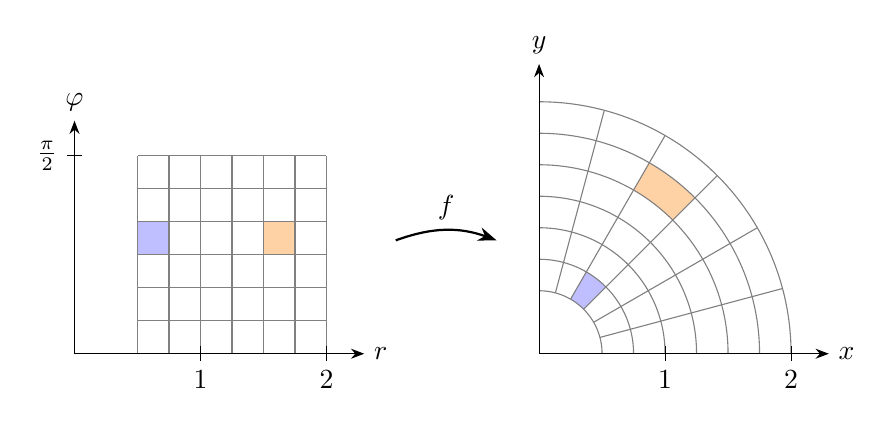
\begin{tikzpicture}[x=1.6cm, y=1.6cm, >=Stealth]
        \fill[orange!35] (1.5,{pi/4}) rectangle (1.75,{pi/3});
        \fill[blue!25] (0.5,{pi/4}) rectangle (0.75,{pi/3});
        \foreach \r in {0.5,0.75,...,2.01}
            \draw[gray] (\r,0) -- (\r,{pi/2});
        \foreach \k in {0,...,6}
            \draw[gray] (0.5,{\k*pi/12}) -- (2,{\k*pi/12});
        \draw[->] (0,0) -- (2.3,0) node[right] {$r$};
        \draw[->] (0,0) -- (0,1.85) node[above] {$\varphi$};
        \draw (0.06,{pi/2}) -- (-0.06,{pi/2}) node[left] {$\frac{\pi}{2}$};
        \foreach \r in {1,2}
            \draw (\r,0.06) -- (\r,-0.06) node[below] {$\r$};
        \draw[->, thick] (2.55,0.9) to[bend left=20] node[above] {$f$} (3.35,0.9);
        \begin{scope}[xshift=5.9cm]
            \fill[orange!35] (45:1.5) arc (45:60:1.5) -- (60:1.75) arc (60:45:1.75) -- cycle;
            \fill[blue!25] (45:0.5) arc (45:60:0.5) -- (60:0.75) arc (60:45:0.75) -- cycle;
            \foreach \r in {0.5,0.75,...,2.01}
                \draw[gray] (\r,0) arc (0:90:\r);
            \foreach \a in {0,15,...,90}
                \draw[gray] (\a:0.5) -- (\a:2);
            \draw[->] (0,0) -- (2.3,0) node[right] {$x$};
            \draw[->] (0,0) -- (0,2.3) node[above] {$y$};
            \foreach \r in {1,2}
                \draw (\r,0.06) -- (\r,-0.06) node[below] {$\r$};
        \end{scope}
    \end{tikzpicture}
    \caption{Polar coordinates $f(r, \varphi) = (r\cos\varphi, r\sin\varphi)$. The grid of rectangles on the left is mapped to the grid of annulus pieces on the right. The two shaded rectangles have the same area, but their images do not: since $\det Df(r, \varphi) = r$, areas are stretched more far from the origin. (The image of $[r_1, r_2] \times [\varphi_1, \varphi_2]$ has the area $\frac{r_1 + r_2}{2}(r_2 - r_1)(\varphi_2 - \varphi_1)$, so the orange image is $\frac{1.625}{0.625} = 2.6$ times as large as the blue one.)}
    \label{L3-fig:polar}
\end{figure}

\begin{remark}[Change of variables]\label{L3-rem:change-of-variables}
    More generally, if $f$ is a differentiable bijection between open subsets $U$ and $V$ of $\mathbb{R}^n$ with a differentiable inverse, then $\int_V g(\mathbf{y}) \, d\mathbf{y} = \int_U g(f(\mathbf{x})) \, |\det Df(\mathbf{x})| \, d\mathbf{x}$ (Theorem~\ref{L3-thm:change-of-variables}). In probability, it says that if a random vector $X$ has the density $p_X$, then $Y = f(X)$ has the density $p_Y$ with $p_Y(f(\mathbf{x})) = \frac{p_X(\mathbf{x})}{|\det Df(\mathbf{x})|}$. Normalizing flows are generative models that turn simple random vectors (e.g., Gaussian ones) into complicated ones in this way. They use neural networks $f$ whose Jacobian determinant is cheap to compute, for example networks with triangular Jacobians, whose determinant is the product of the diagonal entries (Lecture~1).
\end{remark}

\section{The Chain Rule}\label{L3-sec:chain-rule}

Most functions in machine learning are compositions of simpler functions: a neural network is a composition of layers, and its loss is a composition of the network with a loss function. The chain rule tells us how to differentiate compositions.

\begin{theorem}[Chain rule]\label{L3-thm:chain-rule}
    Let $g: D \to \mathbb{R}^m$ with $D \subseteq \mathbb{R}^n$ open, and $f: E \to \mathbb{R}^k$ with $E \subseteq \mathbb{R}^m$ open and $g(D) \subseteq E$. If $g$ is differentiable at $\mathbf{x}$ and $f$ is differentiable at $g(\mathbf{x})$, then $f \circ g$ is differentiable at $\mathbf{x}$, and
    \[D(f \circ g)(\mathbf{x}) = Df(g(\mathbf{x})) \, Dg(\mathbf{x}).\]
    The sizes of the matrices are $(k \times n) = (k \times m)(m \times n)$. In terms of the entries,
    \[\frac{\partial (f \circ g)_i}{\partial x_j}(\mathbf{x}) = \sum_{l=1}^m \frac{\partial f_i}{\partial y_l}(g(\mathbf{x})) \, \frac{\partial g_l}{\partial x_j}(\mathbf{x}),\]
    where $y_1, \ldots, y_m$ denote the variables of $f$.
\end{theorem}

\begin{proof}
    Let $\mathbf{y} = g(\mathbf{x})$, $A = Dg(\mathbf{x})$ and $B = Df(\mathbf{y})$. By assumption,
    \[g(\mathbf{x} + \mathbf{h}) = \mathbf{y} + \mathbf{k}(\mathbf{h}) \quad \text{with } \mathbf{k}(\mathbf{h}) = A\mathbf{h} + \mathbf{r}(\mathbf{h}), \qquad f(\mathbf{y} + \mathbf{k}) = f(\mathbf{y}) + B\mathbf{k} + \mathbf{s}(\mathbf{k}),\]
    where $\frac{\norm{\mathbf{r}(\mathbf{h})}}{\norm{\mathbf{h}}} \to 0$ as $\mathbf{h} \to \mathbf{0}$ and $\frac{\norm{\mathbf{s}(\mathbf{k})}}{\norm{\mathbf{k}}} \to 0$ as $\mathbf{k} \to \mathbf{0}$, with $\mathbf{s}(\mathbf{0}) = \mathbf{0}$. Hence
    \[f(g(\mathbf{x} + \mathbf{h})) = f(\mathbf{y}) + BA\mathbf{h} + \big(B\mathbf{r}(\mathbf{h}) + \mathbf{s}(\mathbf{k}(\mathbf{h}))\big),\]
    and we have to show that the error term in parentheses is $o(\norm{\mathbf{h}})$. We use the spectral norm of Lecture~2, which satisfies $\norm{M\mathbf{v}} \leq \norm{M}_2 \norm{\mathbf{v}}$. First, $\norm{B\mathbf{r}(\mathbf{h})} \leq \norm{B}_2 \norm{\mathbf{r}(\mathbf{h})}$, which is $o(\norm{\mathbf{h}})$. Second, for small $\mathbf{h}$, we have $\norm{\mathbf{r}(\mathbf{h})} \leq \norm{\mathbf{h}}$ and therefore $\norm{\mathbf{k}(\mathbf{h})} \leq (\norm{A}_2 + 1)\norm{\mathbf{h}}$. Let $\varepsilon > 0$. For small $\mathbf{k}$, we have $\norm{\mathbf{s}(\mathbf{k})} \leq \varepsilon \norm{\mathbf{k}}$, so for small $\mathbf{h}$,
    \[\norm{\mathbf{s}(\mathbf{k}(\mathbf{h}))} \leq \varepsilon \norm{\mathbf{k}(\mathbf{h})} \leq \varepsilon (\norm{A}_2 + 1) \norm{\mathbf{h}}.\]
    Since $\varepsilon$ was arbitrary, $\mathbf{s}(\mathbf{k}(\mathbf{h})) = o(\norm{\mathbf{h}})$ as well.
\end{proof}

The chain rule says that the linear approximation of $f \circ g$ is the composition of the linear approximations of $f$ and $g$. Since the matrix of a composition of linear maps is the product of their matrices (Lecture~1), the Jacobian of $f \circ g$ is the product of the Jacobians. For $n = m = k = 1$, it is the familiar rule $(f \circ g)'(x) = f'(g(x)) g'(x)$. Two special cases are particularly important.

\begin{corollary}\label{L3-cor:chain-special}
    \begin{enumerate}
        \item (Functions along curves.) Let $\mathbf{x}: I \to \mathbb{R}^n$, $t \mapsto \mathbf{x}(t) = (x_1(t), \ldots, x_n(t))^\top$, be differentiable on an open interval $I$, and let $f: \mathbb{R}^n \to \mathbb{R}$ be differentiable. Then
        \[\frac{d}{dt} f(\mathbf{x}(t)) = \nabla f(\mathbf{x}(t))^\top \mathbf{x}'(t) = \sum_{i=1}^n \frac{\partial f}{\partial x_i}(\mathbf{x}(t)) \, x_i'(t), \qquad \text{where } \mathbf{x}'(t) = (x_1'(t), \ldots, x_n'(t))^\top.\]
        \item (Gradients of compositions.) Let $g: \mathbb{R}^n \to \mathbb{R}^m$ and $f: \mathbb{R}^m \to \mathbb{R}$ be differentiable. Then
        \[\nabla (f \circ g)(\mathbf{x}) = Dg(\mathbf{x})^\top \, \nabla f(g(\mathbf{x})).\]
    \end{enumerate}
\end{corollary}

\begin{proof}
    (1) The Jacobian of $t \mapsto \mathbf{x}(t)$ is the $n \times 1$ matrix $\mathbf{x}'(t)$, so this is the chain rule with $D f(\mathbf{x}(t)) = \nabla f(\mathbf{x}(t))^\top$. (2) By the chain rule, $D(f \circ g)(\mathbf{x}) = Df(g(\mathbf{x})) Dg(\mathbf{x}) = \nabla f(g(\mathbf{x}))^\top Dg(\mathbf{x})$; now take the transpose.
\end{proof}

Part (2) says that gradients are pulled back through a function by multiplying with the transposed Jacobian. This is the key step of backpropagation (Section~\ref{L3-sec:autodiff}).

\begin{example}\label{L3-ex:chain-curve}
    Let $f(x_1, x_2) = x_1^2 + 2x_2$, and let $\mathbf{x}(t) = (\sin t, \cos t)^\top$ move on the unit circle. Then $\nabla f(\mathbf{x}) = (2x_1, 2)^\top$ and $\mathbf{x}'(t) = (\cos t, -\sin t)^\top$, so
    \[\frac{d}{dt} f(\mathbf{x}(t)) = 2\sin t \cos t - 2\sin t.\]
    We can check this directly: $f(\mathbf{x}(t)) = \sin^2 t + 2\cos t$ has the derivative $2\sin t \cos t - 2\sin t$.
\end{example}

\begin{corollary}[The gradient is orthogonal to level sets]\label{L3-cor:level-sets}
    Let $f: \mathbb{R}^n \to \mathbb{R}$ be differentiable, and let $\mathbf{x}: I \to \mathbb{R}^n$ be a differentiable curve in a level set of $f$, i.e., $f(\mathbf{x}(t)) = c$ for all $t \in I$. Then $\nabla f(\mathbf{x}(t))^\top \mathbf{x}'(t) = 0$ for all $t \in I$.
\end{corollary}

\begin{proof}
    By Corollary~\ref{L3-cor:chain-special}(1), $\nabla f(\mathbf{x}(t))^\top \mathbf{x}'(t)$ is the derivative of the constant function $t \mapsto c$, which is $0$.
\end{proof}

The vector $\mathbf{x}'(t)$ is tangent to the curve, so the gradient is orthogonal to every curve in the level set, i.e., orthogonal to the level set itself; see Figure~\ref{L3-fig:gradient-field}. Together with Theorem~\ref{L3-thm:steepest}, this gives a good picture: the steepest way up a hill is perpendicular to the contour lines of the map, and the gradient is longer where the contour lines are closer together.

\begin{figure}[ht]
    \centering
    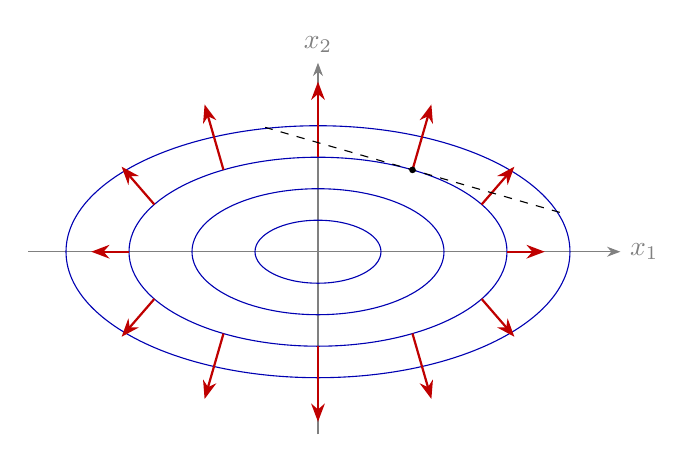
\begin{tikzpicture}[scale=0.8, >=Stealth]
        \draw[->, gray] (-4.6,0) -- (4.8,0) node[right] {$x_1$};
        \draw[->, gray] (0,-2.9) -- (0,3.0) node[above] {$x_2$};
        \foreach \c in {1,2,3,4}
            \draw[blue!70!black] (0,0) ellipse ({\c} and {\c/2});
        \foreach \t in {0,30,...,330}
            \draw[->, red!75!black, thick] ({3*cos(\t)},{1.5*sin(\t)}) -- ++({0.6*cos(\t)},{1.2*sin(\t)});
        \draw[dashed] ({3*cos(60)-0.9*(-3*sin(60))},{1.5*sin(60)-0.9*1.5*cos(60)}) -- ({3*cos(60)+0.9*(-3*sin(60))},{1.5*sin(60)+0.9*1.5*cos(60)});
        \fill ({3*cos(60)},{1.5*sin(60)}) circle (1.5pt);
    \end{tikzpicture}
    \caption{Level curves $x_1^2 + 4x_2^2 = c$ of $f(\mathbf{x}) = x_1^2 + 4x_2^2$ for $c = 1, 4, 9, 16$, and the gradients $\nabla f(\mathbf{x}) = (2x_1, 8x_2)^\top$ (scaled by $0.1$) at points of the level curve $c = 9$. The gradients are orthogonal to the level curve (dashed: the tangent line at one point), and they are longest where the level curves are closest together, on the $x_2$-axis.}
    \label{L3-fig:gradient-field}
\end{figure}

\begin{example}[The gradient of least squares]\label{L3-ex:ls-gradient}
    Let $\Phi \in \mathbb{R}^{N \times d}$ be a design matrix and $\mathbf{y} \in \mathbb{R}^N$ a vector of targets, as in the section on least squares in Lecture~2, and let
    \[L(\boldsymbol{\theta}) = \norm{\mathbf{y} - \Phi\boldsymbol{\theta}}^2, \qquad \boldsymbol{\theta} \in \mathbb{R}^d.\]
    We write $L = f \circ \mathbf{e}$ with the residual $\mathbf{e}(\boldsymbol{\theta}) = \mathbf{y} - \Phi\boldsymbol{\theta}$ and $f(\mathbf{e}) = \norm{\mathbf{e}}^2$. By Example~\ref{L3-ex:affine-jacobian} and Proposition~\ref{L3-prop:basic-gradients}, $D\mathbf{e}(\boldsymbol{\theta}) = -\Phi$ and $Df(\mathbf{e}) = 2\mathbf{e}^\top$. By the chain rule,
    \[DL(\boldsymbol{\theta}) = \underbrace{2(\mathbf{y} - \Phi\boldsymbol{\theta})^\top}_{1 \times N} \, \underbrace{(-\Phi)}_{N \times d}, \qquad \text{so} \qquad \nabla L(\boldsymbol{\theta}) = -2\Phi^\top(\mathbf{y} - \Phi\boldsymbol{\theta}) = 2\Phi^\top(\Phi\boldsymbol{\theta} - \mathbf{y}).\]
    Setting the gradient to zero gives $\Phi^\top\Phi\boldsymbol{\theta} = \Phi^\top\mathbf{y}$, the normal equations, which we found in Lecture~2 with orthogonal projections. Note how writing the sizes of the matrices under the factors checks that the product makes sense. This simple test catches many mistakes in gradient computations.
\end{example}

\begin{example}[Logistic regression]\label{L3-ex:logistic}
    In binary classification, each data point $\mathbf{x} \in \mathbb{R}^n$ has a label $y \in \{0, 1\}$. Logistic regression predicts the probability $p = \sigma(\mathbf{w}^\top \mathbf{x})$ that $y = 1$, where $\sigma$ is the sigmoid function, and it is trained by minimizing the cross-entropy loss, which for one data point is
    \[\ell(\mathbf{w}) = -y \log p - (1 - y) \log(1 - p), \qquad p = \sigma(\mathbf{w}^\top \mathbf{x}).\]
    It is small if the predicted probability of the correct label is close to $1$. We compute the gradient with the chain rule, following the computation $\mathbf{w} \mapsto z = \mathbf{w}^\top \mathbf{x} \mapsto p = \sigma(z) \mapsto \ell$. By Example~\ref{L3-ex:sigmoid}, $\frac{dp}{dz} = p(1 - p)$, so
    \[\frac{d\ell}{dz} = \left(-\frac{y}{p} + \frac{1 - y}{1 - p}\right) p(1 - p) = -y(1 - p) + (1 - y)p = p - y,\]
    and since $Dz(\mathbf{w}) = \mathbf{x}^\top$,
    \[\nabla \ell(\mathbf{w}) = \big(\sigma(\mathbf{w}^\top\mathbf{x}) - y\big) \, \mathbf{x}:\]
    the prediction error times the input. For example, for $\mathbf{x} = (1, 2)^\top$, $y = 1$ and $\mathbf{w} = (0.5, -0.25)^\top$, we have $z = 0$, $p = \frac{1}{2}$, $\ell = \log 2$, and $\nabla \ell(\mathbf{w}) = -\frac{1}{2}(1, 2)^\top = (-0.5, -1)^\top$. A step in the direction $-\nabla\ell(\mathbf{w})$ increases $\mathbf{w}^\top\mathbf{x}$, and hence the predicted probability of the correct label $y = 1$. For a data set $(\mathbf{x}_1, y_1), \ldots, (\mathbf{x}_N, y_N)$ with the average loss $L(\mathbf{w}) = \frac{1}{N}\sum_i \ell_i(\mathbf{w})$, we get
    \[\nabla L(\mathbf{w}) = \frac{1}{N} \sum_{i=1}^N \big(\sigma(\mathbf{w}^\top\mathbf{x}_i) - y_i\big) \mathbf{x}_i = \frac{1}{N} X^\top \big(\sigma(X\mathbf{w}) - \mathbf{y}\big),\]
    where $X \in \mathbb{R}^{N \times n}$ has the rows $\mathbf{x}_i^\top$, and $\sigma$ is applied entrywise.
\end{example}

\section{Gradients with Respect to Matrices}\label{L3-sec:matrix-gradients}

The parameters of a layer of a neural network include a weight matrix $W$, so we need derivatives of functions $f: \mathbb{R}^{m \times n} \to \mathbb{R}$. By Lecture~1, $\mathbb{R}^{m \times n}$ is a vector space isomorphic to $\mathbb{R}^{mn}$, so $f$ is a function of the $mn$ entries of $X$, and we can take the partial derivatives $\frac{\partial f}{\partial X_{ij}}$.

\begin{definition}[Gradient with respect to a matrix]\label{L3-def:matrix-gradient}
    Let $f: \mathbb{R}^{m \times n} \to \mathbb{R}$ be differentiable. The gradient of $f$ at $X$ is the $m \times n$ matrix $\nabla f(X)$ with the entries
    \[\big(\nabla f(X)\big)_{ij} = \frac{\partial f}{\partial X_{ij}}(X).\]
\end{definition}

The gradient has the same shape as $X$. Recall from Lecture~2 the Frobenius inner product $\ip{A}{B} = \tr(A^\top B) = \sum_{i, j} A_{ij} B_{ij}$ on $\mathbb{R}^{m \times n}$, which is the dot product of the lists of entries, and the Frobenius norm $\norm{A}_F = \sqrt{\ip{A}{A}}$. Since $f$ is a differentiable function of $mn$ variables, Proposition~\ref{L3-prop:differentiable} gives
\[f(X + H) = f(X) + \ip{\nabla f(X)}{H} + o(\norm{H}_F),\]
and conversely, if $f(X + H) = f(X) + \ip{G}{H} + o(\norm{H}_F)$ for some matrix $G$, then $G = \nabla f(X)$. This gives a convenient method to compute gradients: expand $f(X + H)$, collect the terms that are linear in $H$, and write them in the form $\ip{G}{H} = \tr(G^\top H)$. The following rules for the trace (Lecture~1) are useful: $\tr(A) = \tr(A^\top)$ and $\tr(AB) = \tr(BA)$, and hence
\[\tr(MH) = \tr(H^\top M^\top) = \ip{M^\top}{H} \qquad \text{for all } M \in \mathbb{R}^{n \times m}, \, H \in \mathbb{R}^{m \times n}.\]

\begin{proposition}\label{L3-prop:matrix-gradients}
    Let $X \in \mathbb{R}^{m \times n}$. Then:
    \begin{enumerate}
        \item $\nabla_X \tr(AX) = A^\top$ for $A \in \mathbb{R}^{n \times m}$, and $\nabla_X (\mathbf{a}^\top X \mathbf{b}) = \mathbf{a}\mathbf{b}^\top$ for $\mathbf{a} \in \mathbb{R}^m$, $\mathbf{b} \in \mathbb{R}^n$;
        \item $\nabla_X \norm{AX - B}_F^2 = 2A^\top(AX - B)$ for $A \in \mathbb{R}^{p \times m}$, $B \in \mathbb{R}^{p \times n}$; in particular, $\nabla_X \norm{X}_F^2 = 2X$;
        \item $\nabla_X \tr(X^\top A X) = (A + A^\top)X$ for $A \in \mathbb{R}^{m \times m}$.
    \end{enumerate}
    Here the subscript in $\nabla_X$ indicates the variable.
\end{proposition}

\begin{proof}
    (1) $\tr(A(X + H)) = \tr(AX) + \tr(AH)$, and $\tr(AH) = \ip{A^\top}{H}$. For the second formula, $\mathbf{a}^\top X \mathbf{b}$ is a $1 \times 1$ matrix, so it equals its trace, and $\tr(\mathbf{a}^\top X \mathbf{b}) = \tr(\mathbf{b}\mathbf{a}^\top X)$; now use the first formula with $A = \mathbf{b}\mathbf{a}^\top$.

    (2) Let $R = AX - B$. Then
    \[\norm{A(X + H) - B}_F^2 = \norm{R + AH}_F^2 = \norm{R}_F^2 + 2\ip{R}{AH} + \norm{AH}_F^2.\]
    The last term is quadratic in $H$, so it is $o(\norm{H}_F)$, and $\ip{R}{AH} = \tr(R^\top A H) = \ip{A^\top R}{H}$. For $A = I$ and $B = 0$, we get $\nabla \norm{X}_F^2 = 2X$.

    (3) $\tr((X + H)^\top A (X + H)) = \tr(X^\top A X) + \tr(H^\top A X) + \tr(X^\top A H) + \tr(H^\top A H)$. The last term is quadratic in $H$, $\tr(H^\top A X) = \ip{H}{AX} = \ip{AX}{H}$, and $\tr(X^\top A H) = \ip{A^\top X}{H}$.
\end{proof}

For $n = 1$, part (3) is Proposition~\ref{L3-prop:basic-gradients}(2). The gradient of the determinant is a little harder to compute.

\begin{lemma}\label{L3-lem:det-identity}
    For every $E \in \mathbb{R}^{n \times n}$, $\det(I + tE) = 1 + t\tr(E) + t^2 q(t)$ for some polynomial $q$. In particular, $\frac{d}{dt}\det(I + tE)\big|_{t = 0} = \tr(E)$.
\end{lemma}

\begin{proof}
    Let $\mu_1, \ldots, \mu_n$ be the complex eigenvalues of $E$, so that $\det(E - \lambda I) = \prod_i (\mu_i - \lambda)$, and $\mu_1 + \cdots + \mu_n = \tr(E)$ by Lecture~1. For $t \neq 0$, we take $\lambda = -\frac{1}{t}$ and get
    \[\det(I + tE) = t^n \det\Big(E + \frac{1}{t} I\Big) = t^n \prod_{i=1}^n \Big(\mu_i + \frac{1}{t}\Big) = \prod_{i=1}^n (1 + t\mu_i),\]
    and this also holds for $t = 0$. Multiplying out the product gives
    \[\det(I + tE) = 1 + t(\mu_1 + \cdots + \mu_n) + t^2 q(t) = 1 + t\tr(E) + t^2 q(t),\]
    where $q$ collects the terms with at least two factors $t\mu_i$. (Its coefficients are real, since $t^2 q(t)$ is the difference of the real polynomials $\det(I + tE)$ and $1 + t\tr(E)$.)
\end{proof}

\begin{proposition}[Jacobi's formula]\label{L3-prop:det-gradient}
    For every invertible matrix $X \in \mathbb{R}^{n \times n}$,
    \[\nabla_X \det(X) = \det(X) \, X^{-\top} \qquad \text{and} \qquad \nabla_X \log|\det(X)| = X^{-\top},\]
    where $X^{-\top} = (X^{-1})^\top$.
\end{proposition}

\begin{proof}
    The determinant is a polynomial in the entries of $X$, so it is differentiable by Theorem~\ref{L3-thm:C1}. For every $H \in \mathbb{R}^{n \times n}$, by Lemma~\ref{L3-lem:det-identity} with $E = X^{-1}H$,
    \[\det(X + tH) = \det(X)\det(I + tX^{-1}H) = \det(X)\big(1 + t\tr(X^{-1}H) + t^2 q(t)\big).\]
    So the directional derivative of $\det$ at $X$ in the direction $H$ is $\det(X)\tr(X^{-1}H) = \ip{\det(X) X^{-\top}}{H}$. By Proposition~\ref{L3-prop:differentiable}, it is also equal to $\ip{\nabla \det(X)}{H}$. Taking for $H$ the matrices with a single entry $1$ and all other entries $0$, we see that the two gradients have the same entries. For the second formula, $\frac{d}{du}\log|u| = \frac{1}{u}$ for $u \neq 0$, so by the chain rule $\nabla \log|\det(X)| = \frac{1}{\det(X)} \nabla\det(X) = X^{-\top}$.
\end{proof}

For $n = 1$, this says that $\frac{d}{dx}\log|x| = \frac{1}{x}$. There is also a direct way to see the first formula: by the cofactor expansion along the $i$-th row, $\frac{\partial \det(X)}{\partial X_{ij}}$ is the cofactor $C_{ij}$, and by Lecture~1, $X^{-1} = \frac{1}{\det(X)}C^\top$, i.e., $\det(X)X^{-\top} = C$. The gradient of $\log|\det|$ appears in the training of Gaussian models and normalizing flows (Remark~\ref{L3-rem:change-of-variables}).

\begin{example}[A linear layer]\label{L3-ex:linear-layer}
    Let $\mathbf{y} = W\mathbf{x} + \mathbf{b}$ with $W \in \mathbb{R}^{m \times n}$, $\mathbf{x} \in \mathbb{R}^n$ and $\mathbf{b} \in \mathbb{R}^m$, and let $L$ be a loss that depends on $\mathbf{y}$ (and maybe on other things). Let $\boldsymbol{\delta} = \nabla_{\mathbf{y}} L \in \mathbb{R}^m$ be the gradient of the loss with respect to the output of the layer. Then
    \[\nabla_W L = \boldsymbol{\delta} \, \mathbf{x}^\top, \qquad \nabla_{\mathbf{b}} L = \boldsymbol{\delta}, \qquad \nabla_{\mathbf{x}} L = W^\top \boldsymbol{\delta}.\]
    Indeed, $y_i = \sum_j W_{ij} x_j + b_i$, and the entry $W_{ij}$ only influences $L$ through $y_i$. So by the chain rule, $\frac{\partial L}{\partial W_{ij}} = \frac{\partial L}{\partial y_i} x_j = \delta_i x_j$, which is the $(i, j)$ entry of the outer product $\boldsymbol{\delta}\mathbf{x}^\top$. Similarly, $\frac{\partial L}{\partial b_i} = \delta_i$, and the last formula is Corollary~\ref{L3-cor:chain-special}(2) with $D\mathbf{y}(\mathbf{x}) = W$. The sizes fit: $\boldsymbol{\delta}\mathbf{x}^\top$ is $m \times n$, like $W$.

    In practice, a layer processes a batch of $N$ inputs at once. If the inputs are the rows of $X \in \mathbb{R}^{N \times n}$, the outputs are the rows of $Y = XW^\top + \mathbf{1}\mathbf{b}^\top \in \mathbb{R}^{N \times m}$, and the loss is the sum of the losses of the data points, then the gradient is the sum of the gradients $\boldsymbol{\delta}_k \mathbf{x}_k^\top$ of the data points:
    \[\nabla_W L = \sum_{k=1}^N \boldsymbol{\delta}_k \mathbf{x}_k^\top = \Delta^\top X, \qquad \nabla_{\mathbf{b}} L = \Delta^\top \mathbf{1},\]
    where $\Delta \in \mathbb{R}^{N \times m}$ has the rows $\boldsymbol{\delta}_k^\top$.
\end{example}

\begin{example}[Softmax with cross-entropy]\label{L3-ex:softmax-ce}
    A classifier with $K$ classes computes a vector of scores $\mathbf{z} \in \mathbb{R}^K$ and predicts the probabilities $\mathbf{p} = \softmax(\mathbf{z})$. If the correct class is $c$, the cross-entropy loss is
    \[\ell(\mathbf{z}) = -\log p_c = -z_c + \log\big(e^{z_1} + \cdots + e^{z_K}\big).\]
    Since $\frac{\partial}{\partial z_k} \log\big(\sum_j e^{z_j}\big) = \frac{e^{z_k}}{\sum_j e^{z_j}} = p_k$, the gradient is
    \[\nabla \ell(\mathbf{z}) = \mathbf{p} - \mathbf{e}_c,\]
    the predicted probabilities minus the ``one-hot'' vector of the correct class. This has the same form as for logistic regression. For example, for $\mathbf{z} = (2, 1, 0)^\top$ and $c = 1$, we get $\mathbf{p} \approx (0.665, 0.245, 0.090)^\top$, $\ell \approx 0.408$, and $\nabla\ell(\mathbf{z}) \approx (-0.335, 0.245, 0.090)^\top$. Gradient descent increases the score of the correct class and decreases the other scores. If the scores come from a linear layer $\mathbf{z} = W\mathbf{x} + \mathbf{b}$, then by Example~\ref{L3-ex:linear-layer}, $\nabla_W \ell = (\mathbf{p} - \mathbf{e}_c)\mathbf{x}^\top$.
\end{example}

We also found that the gradient of the log-sum-exp function $\log(e^{z_1} + \cdots + e^{z_K})$ is $\softmax(\mathbf{z})$. Table~\ref{L3-tab:gradients} collects the gradients of this and the previous sections.

\begin{table}[ht]
    \centering
    \renewcommand{\arraystretch}{1.35}
    \begin{tabular}{lll}
        \hline
        function & gradient & assumptions \\
        \hline
        $\mathbf{a}^\top \mathbf{x}$ & $\mathbf{a}$ & \\
        $\mathbf{x}^\top A \mathbf{x}$ & $(A + A^\top)\mathbf{x}$ & ($= 2A\mathbf{x}$ if $A$ is symmetric) \\
        $\norm{\mathbf{x}}^2$ & $2\mathbf{x}$ & \\
        $\norm{\mathbf{x}}$ & $\mathbf{x} / \norm{\mathbf{x}}$ & $\mathbf{x} \neq \mathbf{0}$ \\
        $\norm{A\mathbf{x} - \mathbf{b}}^2$ & $2A^\top(A\mathbf{x} - \mathbf{b})$ & \\
        $f(g(\mathbf{x}))$ & $Dg(\mathbf{x})^\top \nabla f(g(\mathbf{x}))$ & $f$ scalar-valued \\
        $\log(e^{z_1} + \cdots + e^{z_K})$ & $\softmax(\mathbf{z})$ & \\
        $-\log \softmax(\mathbf{z})_c$ & $\softmax(\mathbf{z}) - \mathbf{e}_c$ & \\
        $\tr(AX)$ & $A^\top$ & \\
        $\mathbf{a}^\top X \mathbf{b}$ & $\mathbf{a}\mathbf{b}^\top$ & \\
        $\norm{AX - B}_F^2$ & $2A^\top(AX - B)$ & \\
        $\tr(X^\top A X)$ & $(A + A^\top)X$ & \\
        $\det(X)$ & $\det(X)X^{-\top}$ & $X$ invertible \\
        $\log|\det(X)|$ & $X^{-\top}$ & $X$ invertible \\
        \hline
    \end{tabular}
    \caption{Some gradients with respect to a vector $\mathbf{x}$ or $\mathbf{z}$, or a matrix $X$.}
    \label{L3-tab:gradients}
\end{table}

\begin{remark}[Derivatives of matrix-valued functions]
    The derivative of a function $F: \mathbb{R}^{m \times n} \to \mathbb{R}^{p \times q}$ at $X$ is a linear map from $\mathbb{R}^{m \times n}$ to $\mathbb{R}^{p \times q}$. Its matrix with respect to the standard bases is a $pq \times mn$ matrix, which is sometimes arranged as a four-dimensional array of numbers (a tensor). In machine learning, we rarely need these large objects explicitly: we only need the gradient of a scalar loss, and the chain rule lets us pass gradients through each function without ever writing down its full Jacobian, as in Example~\ref{L3-ex:linear-layer}. This is how backpropagation works, which is the topic of the next section.
\end{remark}

\section{Backpropagation and Automatic Differentiation}\label{L3-sec:autodiff}

To train a neural network, we need the gradient of the loss with respect to millions of parameters, at every step of training. There are three ways to let a computer compute derivatives.
\begin{itemize}
    \item Symbolic differentiation, as in computer algebra systems, applies the rules of differentiation to formulas. The resulting formulas can become huge, and many programs, with loops and if-statements, are not given by a single formula.
    \item Numerical differentiation uses finite differences (Proposition~\ref{L3-prop:finite-differences}). For a function of $n$ variables, the gradient needs at least $n + 1$ evaluations of the function, which is far too slow for $n = 10^6$, and the result is only approximate.
    \item Automatic differentiation (AD) uses the fact that every program computes a function by a sequence of elementary operations, such as $+$, $\times$, $\exp$ and $\log$, whose derivatives are known. It applies the chain rule to this sequence, with numbers instead of formulas. The result is exact up to rounding errors, and in reverse mode, the cost of the gradient is only a small multiple of the cost of evaluating the function.
\end{itemize}
Backpropagation is reverse-mode automatic differentiation, applied to neural networks.

\subsection{Forward mode and reverse mode}

Let $f = f_L \circ \cdots \circ f_2 \circ f_1$ be a composition of functions $f_l: \mathbb{R}^{n_{l-1}} \to \mathbb{R}^{n_l}$, with $n_0 = n$ and $n_L = m$, such as the layers of a neural network. We evaluate $f$ step by step: $\mathbf{x}_0 = \mathbf{x}$ and $\mathbf{x}_l = f_l(\mathbf{x}_{l-1})$ for $l = 1, \ldots, L$. By the chain rule,
\[Df(\mathbf{x}) = J_L J_{L-1} \cdots J_1, \qquad \text{where } J_l = Df_l(\mathbf{x}_{l-1}) \in \mathbb{R}^{n_l \times n_{l-1}}.\]
Matrix multiplication is associative, so we can compute this product in any order, but the cost depends on the order: multiplying a $p \times q$ matrix by a $q \times r$ matrix costs $pqr$ multiplications.
\begin{itemize}
    \item Forward mode computes $J_L(\cdots(J_2(J_1\mathbf{v})))$ for a vector $\mathbf{v} \in \mathbb{R}^n$, i.e., the Jacobian-vector product $Df(\mathbf{x})\mathbf{v}$, from right to left. Each multiplication can be done together with the evaluation of $f_l$, in the forward direction. For $\mathbf{v} = \mathbf{e}_j$, we get the $j$-th column of $Df(\mathbf{x})$, so the full Jacobian needs $n$ passes.
    \item Reverse mode computes $((\mathbf{u}^\top J_L) J_{L-1}) \cdots J_1$ for a row vector $\mathbf{u}^\top \in \mathbb{R}^{1 \times m}$, i.e., the vector-Jacobian product $\mathbf{u}^\top Df(\mathbf{x})$, from left to right. This goes backwards, from the output to the input, so we first evaluate $f$ and store the intermediate values $\mathbf{x}_0, \ldots, \mathbf{x}_{L-1}$, which we need to compute the Jacobians. For $\mathbf{u} = \mathbf{e}_i$, we get the $i$-th row of $Df(\mathbf{x})$, so the full Jacobian needs $m$ passes.
\end{itemize}
For a loss function, $m = 1$, and a single backward pass with $\mathbf{u} = 1$ gives the whole gradient. For example, if $n_0 = \cdots = n_{L-1} = n$ and $n_L = 1$, then computing the gradient in forward mode needs $n$ passes, each with about $Ln^2$ multiplications, so about $Ln^3$ in total. Reverse mode needs one pass with $L$ vector-matrix products, about $Ln^2$ multiplications, which is comparable to the cost of evaluating $f$ if the $f_l$ are linear layers. For $n = 1000$ and $L = 10$, this is $10^{10}$ versus $10^7$ multiplications. In general, the cost of reverse mode for a scalar function is a small multiple (typically between $2$ and $5$) of the cost of evaluating the function, no matter how many variables it has. The price is memory, since all intermediate values have to be stored. In the language of Lecture~1, reverse mode applies the transposes, or dual maps, $J_1^\top \cdots J_L^\top \mathbf{u}$, which is the rule $(S \circ T)^* = T^* \circ S^*$.

\subsection{Computation graphs}

Most programs are not a simple chain of functions. In general, every intermediate variable $v_j$ is computed from some earlier variables by an elementary operation, which we draw as a computation graph, with an arrow $v_i \to v_j$ if $v_j$ is computed from $v_i$. The two modes of automatic differentiation work as follows.
\begin{itemize}
    \item Forward mode: choose a direction $\dot{\mathbf{x}} = \mathbf{v}$, and compute the derivatives $\dot v_j$ of all intermediate variables in this direction, in the order of evaluation:
    \[\dot v_j = \sum_{i : v_i \to v_j} \frac{\partial v_j}{\partial v_i} \dot v_i.\]
    \item Reverse mode: first evaluate all $v_j$, and then compute the adjoints $\bar v_i = \frac{\partial f}{\partial v_i}$, which describe how the output depends on $v_i$, in the reverse order, starting with $\bar f = 1$:
    \[\bar v_i = \sum_{j : v_i \to v_j} \bar v_j \frac{\partial v_j}{\partial v_i}.\]
    If $v_i$ is used by several later variables, their contributions are added; this is the sum in the chain rule (Theorem~\ref{L3-thm:chain-rule}).
\end{itemize}

\begin{example}\label{L3-ex:autodiff}
    Let $f(x_1, x_2) = \log x_1 + x_1 x_2 - \sin x_2$. Figure~\ref{L3-fig:computation-graph} shows how a computer evaluates $f$, and Table~\ref{L3-tab:autodiff} shows both modes of automatic differentiation at $(x_1, x_2) = (2, 5)$. Forward mode with the direction $\dot{\mathbf{x}} = \mathbf{e}_1$ gives $\frac{\partial f}{\partial x_1} = 5.5$; for $\frac{\partial f}{\partial x_2}$, we need a second pass with $\dot{\mathbf{x}} = \mathbf{e}_2$. Reverse mode gives both partial derivatives in one pass. Note that $\bar x_1$ collects contributions from $v_1$ and $v_2$, since $x_1$ is used to compute both. We check the result: $\frac{\partial f}{\partial x_1} = \frac{1}{x_1} + x_2 = 5.5$ and $\frac{\partial f}{\partial x_2} = x_1 - \cos x_2 \approx 2 - 0.284 = 1.716$.
\end{example}

\begin{figure}[ht]
    \centering
    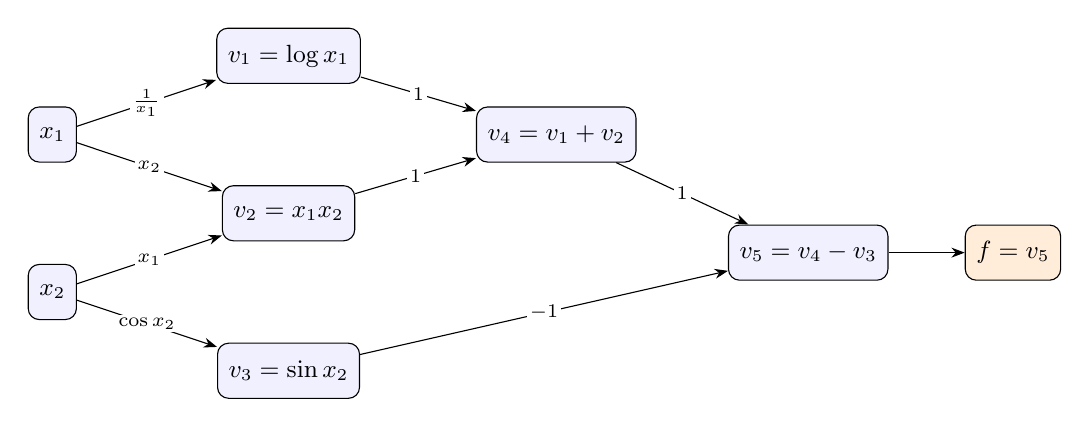
\begin{tikzpicture}[>=Stealth, node distance=1cm,
        var/.style={draw, rounded corners, fill=blue!6, minimum height=0.7cm, inner sep=4pt, font=\small},
        lab/.style={font=\scriptsize, midway, fill=white, inner sep=1pt}]
        \node[var] (x1) at (0,2) {$x_1$};
        \node[var] (x2) at (0,0) {$x_2$};
        \node[var] (v1) at (3,3) {$v_1 = \log x_1$};
        \node[var] (v2) at (3,1) {$v_2 = x_1 x_2$};
        \node[var] (v3) at (3,-1) {$v_3 = \sin x_2$};
        \node[var] (v4) at (6.4,2) {$v_4 = v_1 + v_2$};
        \node[var] (v5) at (9.6,0.5) {$v_5 = v_4 - v_3$};
        \node[var, fill=orange!15] (f) at (12.2,0.5) {$f = v_5$};
        \draw[->] (x1) -- (v1) node[lab] {$\frac{1}{x_1}$};
        \draw[->] (x1) -- (v2) node[lab] {$x_2$};
        \draw[->] (x2) -- (v2) node[lab] {$x_1$};
        \draw[->] (x2) -- (v3) node[lab] {$\cos x_2$};
        \draw[->] (v1) -- (v4) node[lab] {$1$};
        \draw[->] (v2) -- (v4) node[lab] {$1$};
        \draw[->] (v4) -- (v5) node[lab] {$1$};
        \draw[->] (v3) -- (v5) node[lab] {$-1$};
        \draw[->] (v5) -- (f);
    \end{tikzpicture}
    \caption{The computation graph of $f(x_1, x_2) = \log x_1 + x_1 x_2 - \sin x_2$. Each arrow $v_i \to v_j$ is labeled with the local partial derivative $\frac{\partial v_j}{\partial v_i}$.}
    \label{L3-fig:computation-graph}
\end{figure}

\begin{table}[ht]
    \centering
    \renewcommand{\arraystretch}{1.3}
    \begin{tabular}{lll}
        \hline
        evaluation & & forward mode, $\dot{\mathbf{x}} = \mathbf{e}_1$ \\
        \hline
        $x_1 = 2$ & & $\dot x_1 = 1$ \\
        $x_2 = 5$ & & $\dot x_2 = 0$ \\
        $v_1 = \log x_1$ & $= 0.693$ & $\dot v_1 = \dot x_1 / x_1 = 0.5$ \\
        $v_2 = x_1 x_2$ & $= 10$ & $\dot v_2 = \dot x_1 x_2 + x_1 \dot x_2 = 5$ \\
        $v_3 = \sin x_2$ & $= -0.959$ & $\dot v_3 = \cos(x_2)\, \dot x_2 = 0$ \\
        $v_4 = v_1 + v_2$ & $= 10.693$ & $\dot v_4 = \dot v_1 + \dot v_2 = 5.5$ \\
        $v_5 = v_4 - v_3$ & $= 11.652$ & $\dot v_5 = \dot v_4 - \dot v_3 = 5.5$ \\
        \hline
    \end{tabular}
    \qquad
    \begin{tabular}{l}
        \hline
        reverse mode \\
        \hline
        $\bar v_5 = 1$ \\
        $\bar v_4 = \bar v_5 = 1$ \\
        $\bar v_3 = -\bar v_5 = -1$ \\
        $\bar v_2 = \bar v_4 = 1$ \\
        $\bar v_1 = \bar v_4 = 1$ \\
        $\bar x_2 = \bar v_2 x_1 + \bar v_3 \cos x_2 = 1.716$ \\
        $\bar x_1 = \bar v_1 / x_1 + \bar v_2 x_2 = 5.5$ \\
        \hline
    \end{tabular}
    \caption{Automatic differentiation of $f(x_1, x_2) = \log x_1 + x_1 x_2 - \sin x_2$ at $(2, 5)$. Left: evaluation and forward mode, from top to bottom. Right: reverse mode, from top to bottom, i.e., backwards through the computation graph.}
    \label{L3-tab:autodiff}
\end{table}

\subsection{Backpropagation in a neural network}

Consider a neural network with one hidden layer, which maps an input $\mathbf{x} \in \mathbb{R}^n$ to an output $\hat{\mathbf{y}} \in \mathbb{R}^m$, and its squared loss for a target $\mathbf{y} \in \mathbb{R}^m$:
\[\mathbf{z} = W_1 \mathbf{x} + \mathbf{b}_1, \qquad \mathbf{a} = \sigma(\mathbf{z}), \qquad \hat{\mathbf{y}} = W_2 \mathbf{a} + \mathbf{b}_2, \qquad L = \tfrac{1}{2}\norm{\hat{\mathbf{y}} - \mathbf{y}}^2,\]
where $W_1 \in \mathbb{R}^{h \times n}$, $\mathbf{b}_1 \in \mathbb{R}^h$, $W_2 \in \mathbb{R}^{m \times h}$, $\mathbf{b}_2 \in \mathbb{R}^m$, and $\sigma$ is applied entrywise. The forward pass computes and stores $\mathbf{z}$, $\mathbf{a}$, $\hat{\mathbf{y}}$ and $L$. The backward pass computes, using Examples~\ref{L3-ex:linear-layer} and~\ref{L3-ex:entrywise}:
\begin{align*}
    \boldsymbol{\delta}_2 &= \nabla_{\hat{\mathbf{y}}} L = \hat{\mathbf{y}} - \mathbf{y}, \\
    \nabla_{W_2} L &= \boldsymbol{\delta}_2 \mathbf{a}^\top, \qquad \nabla_{\mathbf{b}_2} L = \boldsymbol{\delta}_2, \\
    \nabla_{\mathbf{a}} L &= W_2^\top \boldsymbol{\delta}_2, \\
    \boldsymbol{\delta}_1 &= \nabla_{\mathbf{z}} L = D\sigma(\mathbf{z})^\top \nabla_{\mathbf{a}} L = \sigma'(\mathbf{z}) \odot \big(W_2^\top \boldsymbol{\delta}_2\big), \\
    \nabla_{W_1} L &= \boldsymbol{\delta}_1 \mathbf{x}^\top, \qquad \nabla_{\mathbf{b}_1} L = \boldsymbol{\delta}_1.
\end{align*}
Each line only uses values from the forward pass and from the previous lines. For a deeper network with layers $\mathbf{z}_l = W_l \mathbf{a}_{l-1} + \mathbf{b}_l$, $\mathbf{a}_l = \sigma(\mathbf{z}_l)$, the same pattern repeats: the ``error signals'' $\boldsymbol{\delta}_l = \nabla_{\mathbf{z}_l} L$ satisfy
\[\boldsymbol{\delta}_l = \sigma'(\mathbf{z}_l) \odot \big(W_{l+1}^\top \boldsymbol{\delta}_{l+1}\big), \qquad \nabla_{W_l} L = \boldsymbol{\delta}_l \mathbf{a}_{l-1}^\top, \qquad \nabla_{\mathbf{b}_l} L = \boldsymbol{\delta}_l.\]
The error signals are propagated backwards through the network, which explains the name backpropagation. The backward pass of a layer costs about twice as much as its forward pass: it computes $W_{l+1}^\top\boldsymbol{\delta}_{l+1}$ and the outer product $\boldsymbol{\delta}_l\mathbf{a}_{l-1}^\top$, and each of them costs about as much as the product $W_l\mathbf{a}_{l-1}$ in the forward pass. Machine learning libraries such as PyTorch and JAX implement reverse-mode automatic differentiation for general programs: they record the computation graph during the forward pass, and each elementary operation knows how to compute its vector-Jacobian product.

\begin{remark}[Vanishing and exploding gradients]
    By the recursion above, $\boldsymbol{\delta}_1$ is obtained from $\boldsymbol{\delta}_L$ by multiplying with the matrices $D\sigma(\mathbf{z}_l)^\top W_{l+1}^\top = \diag(\sigma'(\mathbf{z}_l)) W_{l+1}^\top$, once for every layer. For the sigmoid function, $\sigma' \leq \frac{1}{4}$ (Example~\ref{L3-ex:sigmoid}), so unless the weights are large, the gradients of the first layers become tiny in deep networks (vanishing gradients), and these layers hardly learn. If the weight matrices have large norms, the gradients can instead grow exponentially (exploding gradients). Remedies include the ReLU activation function (whose derivative is $1$ for active units), careful initialization of the weights, and residual connections $\mathbf{a}_l = \mathbf{a}_{l-1} + f_l(\mathbf{a}_{l-1})$, whose Jacobian $I + Df_l$ is close to the identity matrix.
\end{remark}

\begin{remark}[Gradient checking]
    Hand-written backward passes are easy to get wrong. To check them, compare the computed gradient $\mathbf{g}$ with central differences $\tilde{g}_i = \frac{f(\mathbf{x} + h\mathbf{e}_i) - f(\mathbf{x} - h\mathbf{e}_i)}{2h}$ for a few random inputs, and compute the relative error $\frac{\norm{\mathbf{g} - \tilde{\mathbf{g}}}}{\norm{\mathbf{g}} + \norm{\tilde{\mathbf{g}}}}$. With $h \approx 10^{-5}$, a relative error around $10^{-8}$ or smaller indicates a correct gradient, while a mistake typically gives a relative error of order $1$.
\end{remark}

\section{Higher Derivatives and Taylor's Theorem}\label{L3-sec:hessian}

The gradient describes how a function changes to first order. To see whether a critical point is a minimum, and how fast optimization algorithms converge, we need the second derivatives, which describe the curvature of the function.

\begin{definition}[Hessian matrix]\label{L3-def:hessian}
    Let $f: D \to \mathbb{R}$ with $D \subseteq \mathbb{R}^n$ open. If the partial derivative $\frac{\partial f}{\partial x_i}$ has a partial derivative with respect to $x_j$, we write
    \[\frac{\partial^2 f}{\partial x_j \partial x_i} = \frac{\partial}{\partial x_j}\left(\frac{\partial f}{\partial x_i}\right), \qquad \frac{\partial^2 f}{\partial x_i^2} = \frac{\partial}{\partial x_i}\left(\frac{\partial f}{\partial x_i}\right).\]
    The function $f$ is twice continuously differentiable if all these second partial derivatives exist and are continuous on $D$. The Hessian matrix of $f$ at $\mathbf{x}$ is the $n \times n$ matrix $\nabla^2 f(\mathbf{x})$ with the entries
    \[\big(\nabla^2 f(\mathbf{x})\big)_{ij} = \frac{\partial^2 f}{\partial x_i \partial x_j}(\mathbf{x}).\]
\end{definition}

\begin{theorem}[Schwarz]\label{L3-thm:schwarz}
    If $f$ is twice continuously differentiable on $D$, then $\frac{\partial^2 f}{\partial x_i \partial x_j} = \frac{\partial^2 f}{\partial x_j \partial x_i}$ for all $i, j$. In particular, the Hessian matrix is symmetric.
\end{theorem}

We do not prove this theorem. The Hessian is the Jacobian of the gradient, $\nabla^2 f(\mathbf{x}) = D(\nabla f)(\mathbf{x})$: the $i$-th row of $D(\nabla f)(\mathbf{x})$ is the derivative of $\frac{\partial f}{\partial x_i}$, with the entries $\frac{\partial^2 f}{\partial x_j \partial x_i}$, which are equal to $\frac{\partial^2 f}{\partial x_i \partial x_j}$ by Schwarz's theorem.

\begin{example}\label{L3-ex:hessian}
    For $f(x_1, x_2) = x_1^2 x_2 + x_1 x_2^3$ (Example~\ref{L3-ex:partials}), we have $\frac{\partial f}{\partial x_1} = 2x_1x_2 + x_2^3$ and $\frac{\partial f}{\partial x_2} = x_1^2 + 3x_1x_2^2$, so
    \[\nabla^2 f(\mathbf{x}) = \begin{pmatrix} 2x_2 & 2x_1 + 3x_2^2 \\ 2x_1 + 3x_2^2 & 6x_1x_2 \end{pmatrix}, \qquad \nabla^2 f(1, 2) = \begin{pmatrix} 4 & 14 \\ 14 & 12 \end{pmatrix}.\]
    As predicted by Schwarz's theorem, the two mixed partial derivatives are equal.
\end{example}

\begin{example}[Hessians in machine learning]\label{L3-ex:ml-hessians}
    \begin{enumerate}
        \item For a quadratic function $f(\mathbf{x}) = \frac{1}{2}\mathbf{x}^\top A\mathbf{x} - \mathbf{b}^\top\mathbf{x} + c$ with a symmetric matrix $A$, Proposition~\ref{L3-prop:basic-gradients} gives $\nabla f(\mathbf{x}) = A\mathbf{x} - \mathbf{b}$, and by Example~\ref{L3-ex:affine-jacobian}, $\nabla^2 f(\mathbf{x}) = A$ for all $\mathbf{x}$. For example, the least squares loss $L(\boldsymbol{\theta}) = \norm{\mathbf{y} - \Phi\boldsymbol{\theta}}^2$ has the gradient $2\Phi^\top\Phi\boldsymbol{\theta} - 2\Phi^\top\mathbf{y}$ and the Hessian $2\Phi^\top\Phi$.
        \item For logistic regression (Example~\ref{L3-ex:logistic}), $\nabla \ell(\mathbf{w}) = (\sigma(\mathbf{w}^\top\mathbf{x}) - y)\mathbf{x}$. Its Jacobian is $\mathbf{x} \cdot \sigma'(\mathbf{w}^\top\mathbf{x})\mathbf{x}^\top$, so $\nabla^2 \ell(\mathbf{w}) = p(1 - p)\mathbf{x}\mathbf{x}^\top$ with $p = \sigma(\mathbf{w}^\top\mathbf{x})$. For a data set, $\nabla^2 L(\mathbf{w}) = \frac{1}{N}\sum_i p_i(1 - p_i)\mathbf{x}_i\mathbf{x}_i^\top = \frac{1}{N} X^\top S X$, where $S = \diag(p_1(1 - p_1), \ldots, p_N(1 - p_N))$.
        \item The log-sum-exp function $\operatorname{lse}(\mathbf{z}) = \log(e^{z_1} + \cdots + e^{z_K})$ has the gradient $\softmax(\mathbf{z})$ (Example~\ref{L3-ex:softmax-ce}), so its Hessian is the Jacobian of the softmax function, $\nabla^2 \operatorname{lse}(\mathbf{z}) = \diag(\mathbf{p}) - \mathbf{p}\mathbf{p}^\top$ with $\mathbf{p} = \softmax(\mathbf{z})$ (Example~\ref{L3-ex:softmax-jacobian}).
    \end{enumerate}
\end{example}

\subsection{Taylor's theorem in several variables}

\begin{theorem}[Second-order Taylor expansion]\label{L3-thm:taylor2}
    Let $f$ be twice continuously differentiable on an open set $D$ that contains the line segment from $\mathbf{x}$ to $\mathbf{x} + \mathbf{h}$. Then there is a $\tau \in (0, 1)$ such that
    \[f(\mathbf{x} + \mathbf{h}) = f(\mathbf{x}) + \nabla f(\mathbf{x})^\top \mathbf{h} + \frac{1}{2}\mathbf{h}^\top \nabla^2 f(\mathbf{x} + \tau\mathbf{h}) \, \mathbf{h}.\]
    Consequently,
    \[f(\mathbf{x} + \mathbf{h}) = f(\mathbf{x}) + \nabla f(\mathbf{x})^\top \mathbf{h} + \frac{1}{2}\mathbf{h}^\top \nabla^2 f(\mathbf{x}) \, \mathbf{h} + o(\norm{\mathbf{h}}^2).\]
\end{theorem}

\begin{proof}
    We reduce to one variable. Let $g(t) = f(\mathbf{x} + t\mathbf{h})$ for $t$ in an open interval containing $[0, 1]$. By the chain rule (Corollary~\ref{L3-cor:chain-special}(1)),
    \[g'(t) = \nabla f(\mathbf{x} + t\mathbf{h})^\top \mathbf{h} = \sum_{i=1}^n \frac{\partial f}{\partial x_i}(\mathbf{x} + t\mathbf{h}) \, h_i,\]
    and applying the chain rule again to each $\frac{\partial f}{\partial x_i}$,
    \[g''(t) = \sum_{i=1}^n \sum_{j=1}^n \frac{\partial^2 f}{\partial x_j \partial x_i}(\mathbf{x} + t\mathbf{h}) \, h_j h_i = \mathbf{h}^\top \nabla^2 f(\mathbf{x} + t\mathbf{h}) \, \mathbf{h}.\]
    By Taylor's theorem in one variable (Theorem~\ref{L3-thm:taylor-1d} with $k = 1$), $g(1) = g(0) + g'(0) + \frac{1}{2}g''(\tau)$ for some $\tau \in (0, 1)$, which is the first formula. For the second formula, the difference between the two quadratic terms is
    \[\tfrac{1}{2}\big|\mathbf{h}^\top \big(\nabla^2 f(\mathbf{x} + \tau\mathbf{h}) - \nabla^2 f(\mathbf{x})\big)\mathbf{h}\big| \leq \tfrac{1}{2}\norm{\nabla^2 f(\mathbf{x} + \tau\mathbf{h}) - \nabla^2 f(\mathbf{x})}_2 \norm{\mathbf{h}}^2\]
    by the Cauchy--Schwarz inequality, and the spectral norm tends to $0$ as $\mathbf{h} \to \mathbf{0}$, since the second partial derivatives are continuous (and the spectral norm is at most the Frobenius norm).
\end{proof}

So near $\mathbf{x}$, $f$ is approximated by the quadratic function
\[f(\mathbf{x} + \mathbf{h}) \approx f(\mathbf{x}) + \nabla f(\mathbf{x})^\top \mathbf{h} + \tfrac{1}{2}\mathbf{h}^\top \nabla^2 f(\mathbf{x})\mathbf{h}.\]
The gradient gives the slope, and the Hessian gives the curvature: for a unit vector $\mathbf{v}$, the number $\mathbf{v}^\top \nabla^2 f(\mathbf{x})\mathbf{v}$ is the second derivative of $t \mapsto f(\mathbf{x} + t\mathbf{v})$ at $t = 0$, i.e., the curvature of $f$ in the direction $\mathbf{v}$. The eigenvalues and eigenvectors of the Hessian describe the curvature in all directions at once; we work this out in Section~\ref{L3-sec:hessian-eigen}, where it is the key to classifying critical points.

\begin{example}\label{L3-ex:taylor2}
    Let $f(x, y) = e^x \cos y$. Then
    \[\nabla f(x, y) = \begin{pmatrix} e^x\cos y \\ -e^x\sin y \end{pmatrix}, \qquad \nabla^2 f(x, y) = \begin{pmatrix} e^x\cos y & -e^x\sin y \\ -e^x\sin y & -e^x\cos y \end{pmatrix},\]
    so at the origin, $f = 1$, $\nabla f = (1, 0)^\top$ and $\nabla^2 f = \diag(1, -1)$. The second-order approximation is
    \[e^x \cos y \approx 1 + x + \tfrac{1}{2}(x^2 - y^2).\]
    At $(0.1, 0.2)$, it gives $1.085$, while the linear approximation $1 + x$ gives $1.1$, and the exact value is $1.0831\ldots$.
\end{example}

There are also Taylor expansions of higher order, which use all partial derivatives of order $k$. They are rarely needed in machine learning, and we do not discuss them.

\section{Unconstrained Optimization}\label{L3-sec:optimization}

We now use derivatives to minimize functions, which is how models are trained. Maximizing $f$ is the same as minimizing $-f$, so we only discuss minimization.

\begin{definition}[Minima and critical points]\label{L3-def:minimum}
    Let $f: D \to \mathbb{R}$ with $D \subseteq \mathbb{R}^n$ open.
    \begin{enumerate}
        \item A point $\mathbf{x}^* \in D$ is a global minimum (or global minimizer) of $f$ if $f(\mathbf{x}^*) \leq f(\mathbf{x})$ for all $\mathbf{x} \in D$, and a local minimum if there is an $r > 0$ such that $f(\mathbf{x}^*) \leq f(\mathbf{x})$ for all $\mathbf{x} \in D$ with $\norm{\mathbf{x} - \mathbf{x}^*} < r$. It is a strict local minimum if moreover $f(\mathbf{x}^*) < f(\mathbf{x})$ for these $\mathbf{x} \neq \mathbf{x}^*$. Maxima are defined in the same way.
        \item If $f$ is differentiable, a point $\mathbf{x}^*$ with $\nabla f(\mathbf{x}^*) = \mathbf{0}$ is called a critical point (or stationary point) of $f$.
    \end{enumerate}
    We write $\argmin_{\mathbf{x}} f(\mathbf{x})$ for the set of global minima of $f$, or for the global minimum if it is unique.
\end{definition}

\begin{theorem}[First-order condition]\label{L3-thm:first-order}
    If $f$ is differentiable and $\mathbf{x}^*$ is a local minimum of $f$, then $\nabla f(\mathbf{x}^*) = \mathbf{0}$.
\end{theorem}

\begin{proof}
    Suppose that $\mathbf{g} = \nabla f(\mathbf{x}^*) \neq \mathbf{0}$. By Proposition~\ref{L3-prop:differentiable}, the directional derivative of $f$ at $\mathbf{x}^*$ in the direction $-\mathbf{g}$ is $\nabla f(\mathbf{x}^*)^\top(-\mathbf{g}) = -\norm{\mathbf{g}}^2 < 0$. So $\frac{f(\mathbf{x}^* - t\mathbf{g}) - f(\mathbf{x}^*)}{t} < 0$ for all small $t > 0$, i.e., $f(\mathbf{x}^* - t\mathbf{g}) < f(\mathbf{x}^*)$, and $\mathbf{x}^*$ is not a local minimum.
\end{proof}

The same holds for local maxima. The converse is false: a critical point can be a local minimum, a local maximum, or neither. For example, the origin is a critical point of $g(x, y) = x^2 - y^2$ (Figure~\ref{L3-fig:level-sets}), but $g$ increases along the $x$-axis and decreases along the $y$-axis. A critical point that is neither a local minimum nor a local maximum is called a saddle point. To tell these cases apart, we look at the second-order term of the Taylor expansion, and in particular at the eigenvalues of the Hessian.

\subsection{The second-order test}\label{L3-sec:hessian-eigen}

Let $\nabla f(\mathbf{x}^*) = \mathbf{0}$, and let $H = \nabla^2 f(\mathbf{x}^*)$. Since the gradient vanishes, Theorem~\ref{L3-thm:taylor2} gives
\[f(\mathbf{x}^* + \mathbf{h}) = f(\mathbf{x}^*) + \tfrac{1}{2}\mathbf{h}^\top H\mathbf{h} + o(\norm{\mathbf{h}}^2),\]
so near $\mathbf{x}^*$, the shape of $f$ is described by the quadratic form $\mathbf{h}^\top H\mathbf{h}$. The Hessian is symmetric, so by the spectral theorem (Lecture~2) it has an orthonormal basis of eigenvectors $\mathbf{q}_1, \ldots, \mathbf{q}_n$, with real eigenvalues $\lambda_1 \geq \cdots \geq \lambda_n$, and $H = Q\Lambda Q^\top$. Let us measure the displacement $\mathbf{h}$ in this basis: $\mathbf{h} = y_1\mathbf{q}_1 + \cdots + y_n\mathbf{q}_n$, i.e., $\mathbf{y} = Q^\top\mathbf{h}$. Then $H\mathbf{h} = \sum_i \lambda_i y_i\mathbf{q}_i$, and since the $\mathbf{q}_i$ are orthonormal,
\[\mathbf{h}^\top H\mathbf{h} = \lambda_1 y_1^2 + \lambda_2 y_2^2 + \cdots + \lambda_n y_n^2 \qquad \text{and} \qquad \norm{\mathbf{h}}^2 = y_1^2 + \cdots + y_n^2.\]
Therefore, near the critical point,
\[f(\mathbf{x}^* + y_1\mathbf{q}_1 + \cdots + y_n\mathbf{q}_n) \approx f(\mathbf{x}^*) + \tfrac{1}{2}\big(\lambda_1 y_1^2 + \lambda_2 y_2^2 + \cdots + \lambda_n y_n^2\big).\]
In the coordinates given by the eigenvectors, the mixed terms $y_i y_j$ disappear: near a critical point, $f$ looks like a sum of $n$ independent parabolas, one for each eigenvector. Along the line through $\mathbf{x}^*$ in the direction $\mathbf{q}_i$,
\[f(\mathbf{x}^* + t\mathbf{q}_i) \approx f(\mathbf{x}^*) + \tfrac{1}{2}\lambda_i t^2,\]
a parabola that opens upward if $\lambda_i > 0$ and downward if $\lambda_i < 0$. So the eigenvalue $\lambda_i$ is the curvature of $f$ in the direction $\mathbf{q}_i$, i.e., the second derivative of $t \mapsto f(\mathbf{x}^* + t\mathbf{q}_i)$ at $t = 0$. The eigenvectors are called the principal directions (or principal axes) of $f$ at $\mathbf{x}^*$. In any other unit direction $\mathbf{v}$, with $\mathbf{y} = Q^\top\mathbf{v}$, the curvature is $\mathbf{v}^\top H\mathbf{v} = \sum_i \lambda_i y_i^2$ with $\sum_i y_i^2 = 1$, a weighted average of the eigenvalues; so it lies between $\lambda_n$ and $\lambda_1$, as for the Rayleigh quotient in Lecture~2.

Hence the signs of the eigenvalues determine the shape of $f$ near a critical point (Figure~\ref{L3-fig:hessian-shapes} and Table~\ref{L3-tab:second-order}). If all eigenvalues are positive, $f$ curves upward in every direction, like a bowl, and $\mathbf{x}^*$ is a minimum. If all are negative, $f$ curves downward in every direction, like an upside-down bowl, and $\mathbf{x}^*$ is a maximum. If there are eigenvalues of both signs, $f$ curves upward in some directions and downward in others, like a saddle or a mountain pass. And if some eigenvalues are $0$, then $f$ is flat to second order in these directions, like a trough, and the quadratic approximation cannot decide what happens: this depends on the terms of higher order.

\begin{figure}[ht]
    \centering
    \pgfplotsset{hessplot/.style={x={(1.95cm,-0.65cm)}, y={(1.3cm,1.24cm)}, z={(0cm,0.98cm)}, axis lines=none, colormap/viridis}}
    \begin{tikzpicture}
        \begin{axis}[hessplot]
            \addplot3[surf, shader=faceted, draw=black!25, line width=0.05pt, domain=0:1, y domain=0:360, samples=11, samples y=49, z buffer=sort] ({x*cos(y)}, {x*sin(y)}, {x^2*cos(y)^2 + 1.5*x^2*sin(y)^2});
            \addplot3[orange!85!black, very thick, domain=-1:1, samples y=0, samples=30] ({x}, {0}, {x^2});
            \addplot3[orange!85!black, very thick, domain=-1:1, samples y=0, samples=30] ({0}, {x}, {1.5*x^2});
        \end{axis}
    \end{tikzpicture}\hfill
    \begin{tikzpicture}
        \begin{axis}[hessplot]
            \addplot3[surf, shader=faceted, draw=black!25, line width=0.05pt, domain=0:1, y domain=0:360, samples=11, samples y=49, z buffer=sort] ({x*cos(y)}, {x*sin(y)}, {x^2*cos(y)^2 - x^2*sin(y)^2});
            \addplot3[orange!85!black, very thick, domain=-1:1, samples y=0, samples=30] ({x}, {0}, {x^2});
            \addplot3[violet, very thick, domain=-1:1, samples y=0, samples=30] ({0}, {x}, {-x^2});
        \end{axis}
    \end{tikzpicture}\hfill
    \begin{tikzpicture}
        \begin{axis}[hessplot]
            \addplot3[surf, shader=faceted, draw=black!25, line width=0.05pt, domain=0:1, y domain=0:360, samples=11, samples y=49, z buffer=sort] ({x*cos(y)}, {x*sin(y)}, {x^2*cos(y)^2});
            \addplot3[orange!85!black, very thick, domain=-1:1, samples y=0, samples=30] ({x}, {0}, {x^2});
            \addplot3[black!70, very thick, domain=-1:1, samples y=0, samples=30] ({0}, {x}, {0});
        \end{axis}
    \end{tikzpicture}
    \caption{The quadratic approximation $f(\mathbf{x}^*) + \frac{1}{2}(\lambda_1 y_1^2 + \lambda_2 y_2^2)$ of a function near a critical point, in the coordinates $y_1, y_2$ along the eigenvectors of the Hessian. The curves are the parabolas $\frac{1}{2}\lambda_i t^2$ along the eigenvectors: orange for $\lambda_i > 0$, violet for $\lambda_i < 0$, and gray for $\lambda_i = 0$. Left: $\lambda_1, \lambda_2 > 0$, a bowl (local minimum). Middle: $\lambda_1 > 0 > \lambda_2$, a saddle (saddle point). Right: $\lambda_1 > 0$ and $\lambda_2 = 0$, a trough (the second-order test is inconclusive).}
    \label{L3-fig:hessian-shapes}
\end{figure}

\begin{theorem}[Second-order test]\label{L3-thm:second-order}
    Let $f$ be twice continuously differentiable on $D$, let $\nabla f(\mathbf{x}^*) = \mathbf{0}$, and let $\lambda_1 \geq \cdots \geq \lambda_n$ be the eigenvalues of the Hessian $\nabla^2 f(\mathbf{x}^*)$.
    \begin{enumerate}
        \item If all eigenvalues are positive ($\lambda_n > 0$), then $\mathbf{x}^*$ is a strict local minimum.
        \item If all eigenvalues are negative ($\lambda_1 < 0$), then $\mathbf{x}^*$ is a strict local maximum.
        \item If there are positive and negative eigenvalues ($\lambda_1 > 0 > \lambda_n$), then $\mathbf{x}^*$ is a saddle point: $f$ increases along every eigenvector with a positive eigenvalue, and decreases along every eigenvector with a negative eigenvalue.
        \item Conversely, if $\mathbf{x}^*$ is a local minimum, then all eigenvalues are $\geq 0$, and if $\mathbf{x}^*$ is a local maximum, then all eigenvalues are $\leq 0$.
    \end{enumerate}
\end{theorem}

\begin{proof}
    Let $H = \nabla^2 f(\mathbf{x}^*)$, and write $f(\mathbf{x}^* + \mathbf{h}) = f(\mathbf{x}^*) + \frac{1}{2}\mathbf{h}^\top H\mathbf{h} + r(\mathbf{h})$ with $r(\mathbf{h}) = o(\norm{\mathbf{h}}^2)$, as above.

    (1) In the coordinates $\mathbf{y} = Q^\top\mathbf{h}$, we have $\mathbf{h}^\top H\mathbf{h} = \sum_i \lambda_i y_i^2 \geq \lambda_n \sum_i y_i^2 = \lambda_n\norm{\mathbf{h}}^2$: in every direction, $f$ curves upward at least as much as along $\mathbf{q}_n$. For all sufficiently small $\mathbf{h} \neq \mathbf{0}$, we have $|r(\mathbf{h})| \leq \frac{1}{4}\lambda_n\norm{\mathbf{h}}^2$, and hence $f(\mathbf{x}^* + \mathbf{h}) \geq f(\mathbf{x}^*) + \frac{1}{4}\lambda_n\norm{\mathbf{h}}^2 > f(\mathbf{x}^*)$.

    (2) Apply (1) to $-f$, whose Hessian has the eigenvalues $-\lambda_i$.

    (3) Let $\mathbf{q}$ be a unit eigenvector with eigenvalue $\lambda \neq 0$. Then $f(\mathbf{x}^* + t\mathbf{q}) = f(\mathbf{x}^*) + \frac{1}{2}\lambda t^2 + r(t\mathbf{q})$, and $|r(t\mathbf{q})| < \frac{1}{2}|\lambda| t^2$ for all small $t \neq 0$. So for all small $t \neq 0$, $f(\mathbf{x}^* + t\mathbf{q}) > f(\mathbf{x}^*)$ if $\lambda > 0$, and $f(\mathbf{x}^* + t\mathbf{q}) < f(\mathbf{x}^*)$ if $\lambda < 0$. If both signs occur, there are points with larger and points with smaller values arbitrarily close to $\mathbf{x}^*$, so $\mathbf{x}^*$ is neither a local minimum nor a local maximum.

    (4) If some eigenvalue were negative, then by the argument of (3), there would be points with smaller values arbitrarily close to $\mathbf{x}^*$, so $\mathbf{x}^*$ would not be a local minimum. The case of a local maximum is the same.
\end{proof}

In the language of Lecture~2, the Hessian in (1) is positive definite, in (2) negative definite, and in (3) indefinite, and (4) says that the Hessian at a local minimum is positive semidefinite. If some eigenvalues are $0$ and all others have the same sign, the test is inconclusive: $x^4$, $-x^4$ and $x^3$ all have the critical point $0$ with second derivative $0$, but the first has a minimum there, the second a maximum, and the third neither (see also Exercise~\ref{L3-ex3:inconclusive}).

For $n = 2$, we do not even need to compute the eigenvalues, since $\lambda_1\lambda_2 = \det(H)$ and $\lambda_1 + \lambda_2 = \tr(H)$ (Lecture~1). If $\det(H) < 0$, the eigenvalues have opposite signs, and the critical point is a saddle point. If $\det(H) > 0$, they have the same sign, which is the sign of $\tr(H)$: the critical point is a strict local minimum if $\tr(H) > 0$, and a strict local maximum if $\tr(H) < 0$.

\begin{table}[ht]
    \centering
    \renewcommand{\arraystretch}{1.3}
    \begin{tabular}{llll}
        \hline
        eigenvalues of $\nabla^2 f(\mathbf{x}^*)$ & graph near $\mathbf{x}^*$ & level curves & $\mathbf{x}^*$ is a \\
        \hline
        all positive & bowl & ellipses & strict local minimum \\
        all negative & upside-down bowl & ellipses & strict local maximum \\
        positive and negative & saddle & hyperbolas & saddle point \\
        some zero, the rest of one sign & trough & parallel lines & (test inconclusive) \\
        \hline
    \end{tabular}
    \caption{The second-order test at a critical point $\mathbf{x}^*$. The shape of the graph and the level curves (for $n = 2$) are those of the quadratic approximation $f(\mathbf{x}^*) + \frac{1}{2}(\lambda_1 y_1^2 + \cdots + \lambda_n y_n^2)$.}
    \label{L3-tab:second-order}
\end{table}

The eigenvalues also describe the level sets near a strict local minimum. For $c > 0$, the level set $\frac{1}{2}(\lambda_1 y_1^2 + \cdots + \lambda_n y_n^2) = c$ of the quadratic approximation is an ellipse (for $n = 2$) or an ellipsoid, whose axes point in the directions of the eigenvectors $\mathbf{q}_i$ and have the half-lengths $\sqrt{2c/\lambda_i}$, as in the section on the spectral theorem in Lecture~2. So the level curves around a minimum are approximately ellipses that are long in directions of small curvature and short in directions of large curvature. The ratio of the longest and the shortest axis is $\sqrt{\lambda_1/\lambda_n}$, the square root of the condition number of the Hessian, and we will see in Section~\ref{L3-sec:gd} that this elongation determines how fast gradient descent converges. Around a saddle point in the plane, the level curves of the quadratic approximation are hyperbolas, as for $x^2 - y^2$ in Figure~\ref{L3-fig:level-sets}.

\begin{example}\label{L3-ex:critical-points}
    Let $f(x, y) = x^3 + y^3 - 3xy$. Its gradient is $\nabla f(x, y) = (3x^2 - 3y, \, 3y^2 - 3x)^\top$, so at a critical point, $y = x^2$ and $x = y^2 = x^4$. Hence $x = 0$ or $x^3 = 1$, i.e., $x = 1$, and the critical points are $(0, 0)$ and $(1, 1)$. The Hessian is
    \[\nabla^2 f(x, y) = \begin{pmatrix} 6x & -3 \\ -3 & 6y \end{pmatrix}.\]
    \begin{itemize}
        \item At $(1, 1)$, the Hessian $\begin{pmatrix} 6 & -3 \\ -3 & 6 \end{pmatrix}$ has the eigenvector $(1, 1)^\top$ with eigenvalue $3$, and the eigenvector $(1, -1)^\top$ with eigenvalue $9$. Both eigenvalues are positive, so $(1, 1)$ is a strict local minimum, with $f(1, 1) = -1$. The curvature across the diagonal is three times as large as the curvature along it, so the level curves around $(1, 1)$ are approximately ellipses that are elongated in the direction of the diagonal, with axes in the ratio $\sqrt{9/3} = \sqrt{3}$ (Figure~\ref{L3-fig:critical-points}). The minimum is not global, since $f(x, 0) = x^3 \to -\infty$ as $x \to -\infty$.
        \item At $(0, 0)$, the Hessian $\begin{pmatrix} 0 & -3 \\ -3 & 0 \end{pmatrix}$ has the eigenvector $(1, 1)^\top$ with eigenvalue $-3$, and the eigenvector $(1, -1)^\top$ with eigenvalue $3$. So the origin is a saddle point: $f$ decreases along the diagonal $y = x$ and increases along the diagonal $y = -x$. Indeed, $f(t, t) = 2t^3 - 3t^2 \approx -3t^2$ and $f(t, -t) = 3t^2$ for small $t$, which are the parabolas $\frac{1}{2}\lambda t^2 \norm{\mathbf{v}}^2$ for $\mathbf{v} = (1, \pm 1)^\top$. Note that both diagonal entries of the Hessian are $0$: along the coordinate axes, $f(t, 0) = f(0, t) = t^3$ has no curvature at $t = 0$, and we would not see the saddle at all. As in Example~\ref{L3-ex:xy}, looking along the coordinate axes is not enough; the eigenvectors show the directions in which $f$ really curves.
    \end{itemize}
    The level set $f = 0$ is the folium of Descartes $x^3 + y^3 = 3xy$, which crosses itself at the saddle point. Near the origin, it looks like the zero set of the quadratic approximation $\frac{1}{2}\mathbf{h}^\top H\mathbf{h} = -3xy$, which consists of the two coordinate axes.
\end{example}

\begin{figure}[ht]
    \centering
    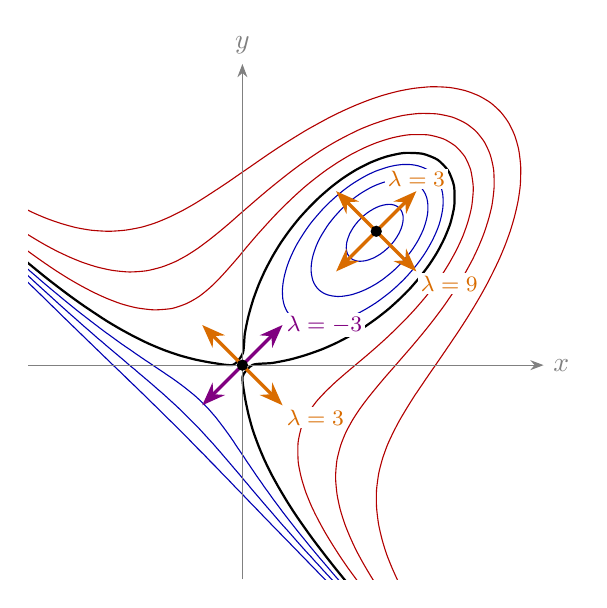
\begin{tikzpicture}[scale=1.7, >=Stealth]
        \begin{scope}
            \clip (-1.6,-1.6) rectangle (2.1,2.1);
            \draw[blue!70!black] plot[smooth, tension=0.4] coordinates {(-1.650,0.666) (-1.618,0.635) (-1.587,0.604) (-1.555,0.573) (-1.523,0.542) (-1.491,0.511) (-1.460,0.480) (-1.428,0.449) (-1.396,0.418) (-1.364,0.386) (-1.332,0.355) (-1.299,0.323) (-1.266,0.291) (-1.234,0.260) (-1.201,0.228) (-1.168,0.196) (-1.136,0.165) (-1.104,0.134) (-1.073,0.104) (-1.041,0.073) (-1.009,0.042) (-0.978,0.012) (-0.945,-0.020) (-0.912,-0.051) (-0.879,-0.083) (-0.847,-0.115) (-0.814,-0.146) (-0.781,-0.178) (-0.749,-0.209) (-0.717,-0.240) (-0.686,-0.271) (-0.654,-0.302) (-0.622,-0.333) (-0.591,-0.364) (-0.559,-0.396) (-0.527,-0.427) (-0.495,-0.459) (-0.464,-0.490) (-0.432,-0.522) (-0.400,-0.554) (-0.369,-0.586) (-0.337,-0.619) (-0.305,-0.651) (-0.273,-0.683) (-0.242,-0.716) (-0.210,-0.748) (-0.178,-0.781) (-0.148,-0.813) (-0.117,-0.844) (-0.086,-0.876) (-0.056,-0.908) (-0.025,-0.939) (0.006,-0.971) (0.037,-1.004) (0.069,-1.037) (0.101,-1.070) (0.133,-1.103) (0.164,-1.136) (0.196,-1.168) (0.226,-1.200) (0.257,-1.231) (0.288,-1.263) (0.319,-1.295) (0.350,-1.326) (0.380,-1.358) (0.412,-1.390) (0.443,-1.423) (0.475,-1.455) (0.507,-1.488) (0.539,-1.520) (0.570,-1.553) (0.602,-1.585) (0.634,-1.617) (0.666,-1.650) (0.666,-1.650)};
            \draw[blue!70!black] plot[smooth, tension=0.4] coordinates {(0.849,0.780) (0.837,0.784) (0.824,0.789) (0.811,0.798) (0.803,0.805) (0.793,0.818) (0.786,0.830) (0.781,0.843) (0.778,0.856) (0.776,0.875) (0.777,0.894) (0.779,0.913) (0.782,0.926) (0.786,0.941) (0.792,0.957) (0.797,0.970) (0.802,0.983) (0.809,0.995) (0.816,1.008) (0.824,1.021) (0.830,1.031) (0.837,1.040) (0.846,1.053) (0.856,1.064) (0.862,1.072) (0.873,1.084) (0.881,1.092) (0.892,1.103) (0.900,1.111) (0.913,1.122) (0.922,1.129) (0.932,1.137) (0.945,1.146) (0.957,1.154) (0.968,1.160) (0.979,1.167) (0.991,1.173) (1.004,1.179) (1.020,1.186) (1.033,1.190) (1.046,1.194) (1.065,1.198) (1.078,1.200) (1.097,1.201) (1.116,1.200) (1.129,1.197) (1.144,1.192) (1.156,1.186) (1.167,1.178) (1.178,1.167) (1.186,1.156) (1.192,1.144) (1.197,1.129) (1.200,1.116) (1.201,1.097) (1.200,1.078) (1.198,1.065) (1.194,1.046) (1.190,1.033) (1.186,1.020) (1.179,1.004) (1.173,0.991) (1.167,0.979) (1.160,0.968) (1.154,0.957) (1.146,0.945) (1.137,0.932) (1.129,0.922) (1.122,0.913) (1.111,0.900) (1.103,0.892) (1.092,0.881) (1.084,0.873) (1.072,0.862) (1.064,0.856) (1.053,0.846) (1.040,0.837) (1.031,0.830) (1.021,0.824) (1.008,0.816) (0.995,0.809) (0.983,0.802) (0.970,0.797) (0.957,0.792) (0.941,0.786) (0.926,0.782) (0.913,0.779) (0.894,0.777) (0.875,0.776) (0.856,0.778) (0.849,0.780)} -- cycle;
            \draw[blue!70!black] plot[smooth, tension=0.4] coordinates {(-1.650,0.713) (-1.618,0.684) (-1.585,0.653) (-1.551,0.621) (-1.517,0.590) (-1.485,0.561) (-1.453,0.532) (-1.419,0.501) (-1.384,0.469) (-1.352,0.440) (-1.320,0.412) (-1.285,0.380) (-1.250,0.350) (-1.219,0.322) (-1.184,0.291) (-1.149,0.261) (-1.117,0.233) (-1.082,0.202) (-1.047,0.173) (-1.015,0.145) (-0.978,0.114) (-0.946,0.087) (-0.910,0.057) (-0.876,0.028) (-0.843,-0.001) (-0.806,-0.031) (-0.775,-0.058) (-0.738,-0.089) (-0.705,-0.117) (-0.671,-0.146) (-0.635,-0.178) (-0.603,-0.205) (-0.570,-0.235) (-0.535,-0.267) (-0.502,-0.297) (-0.470,-0.327) (-0.438,-0.358) (-0.407,-0.389) (-0.375,-0.421) (-0.343,-0.453) (-0.311,-0.487) (-0.280,-0.521) (-0.251,-0.553) (-0.222,-0.584) (-0.191,-0.620) (-0.161,-0.654) (-0.134,-0.686) (-0.102,-0.723) (-0.074,-0.756) (-0.045,-0.790) (-0.015,-0.825) (0.012,-0.858) (0.044,-0.895) (0.070,-0.927) (0.101,-0.963) (0.130,-0.997) (0.158,-1.030) (0.189,-1.066) (0.217,-1.098) (0.247,-1.133) (0.277,-1.168) (0.305,-1.200) (0.336,-1.234) (0.367,-1.269) (0.395,-1.301) (0.424,-1.334) (0.456,-1.370) (0.486,-1.403) (0.515,-1.434) (0.545,-1.468) (0.577,-1.502) (0.607,-1.536) (0.637,-1.568) (0.666,-1.599) (0.697,-1.633) (0.713,-1.650)};
            \draw[blue!70!black] plot[smooth, tension=0.4] coordinates {(0.710,0.513) (0.672,0.517) (0.634,0.526) (0.605,0.539) (0.577,0.558) (0.558,0.577) (0.539,0.605) (0.526,0.634) (0.517,0.672) (0.513,0.710) (0.515,0.748) (0.520,0.786) (0.529,0.824) (0.539,0.856) (0.551,0.889) (0.564,0.919) (0.580,0.951) (0.596,0.979) (0.614,1.008) (0.630,1.033) (0.648,1.059) (0.668,1.084) (0.689,1.110) (0.710,1.133) (0.729,1.154) (0.754,1.179) (0.775,1.198) (0.799,1.219) (0.824,1.240) (0.849,1.259) (0.875,1.277) (0.901,1.294) (0.932,1.312) (0.957,1.326) (0.989,1.341) (1.021,1.354) (1.053,1.365) (1.091,1.376) (1.125,1.382) (1.167,1.386) (1.211,1.385) (1.249,1.377) (1.281,1.365) (1.306,1.351) (1.332,1.329) (1.351,1.306) (1.368,1.275) (1.379,1.243) (1.385,1.205) (1.386,1.160) (1.382,1.122) (1.374,1.084) (1.363,1.046) (1.352,1.014) (1.338,0.983) (1.325,0.956) (1.309,0.926) (1.293,0.900) (1.275,0.872) (1.256,0.845) (1.236,0.820) (1.217,0.797) (1.197,0.773) (1.173,0.748) (1.154,0.729) (1.129,0.706) (1.105,0.685) (1.081,0.666) (1.056,0.646) (1.029,0.627) (1.002,0.609) (0.976,0.594) (0.945,0.577) (0.918,0.564) (0.888,0.551) (0.856,0.539) (0.818,0.527) (0.784,0.520) (0.742,0.514) (0.710,0.513)} -- cycle;
            \draw[blue!70!black] plot[smooth, tension=0.4] coordinates {(-1.650,0.759) (-1.616,0.729) (-1.580,0.697) (-1.548,0.670) (-1.514,0.640) (-1.479,0.610) (-1.447,0.583) (-1.409,0.551) (-1.377,0.525) (-1.340,0.494) (-1.307,0.467) (-1.270,0.437) (-1.238,0.411) (-1.200,0.381) (-1.166,0.355) (-1.130,0.327) (-1.092,0.298) (-1.058,0.272) (-1.022,0.245) (-0.984,0.218) (-0.946,0.190) (-0.910,0.164) (-0.874,0.139) (-0.837,0.114) (-0.800,0.088) (-0.762,0.062) (-0.724,0.036) (-0.686,0.011) (-0.648,-0.015) (-0.610,-0.040) (-0.572,-0.066) (-0.533,-0.092) (-0.495,-0.119) (-0.458,-0.146) (-0.424,-0.172) (-0.388,-0.201) (-0.354,-0.229) (-0.319,-0.261) (-0.287,-0.292) (-0.256,-0.324) (-0.228,-0.356) (-0.197,-0.392) (-0.171,-0.426) (-0.142,-0.464) (-0.115,-0.501) (-0.089,-0.537) (-0.064,-0.574) (-0.039,-0.612) (-0.013,-0.650) (0.012,-0.687) (0.037,-0.725) (0.063,-0.763) (0.088,-0.800) (0.114,-0.838) (0.141,-0.876) (0.167,-0.914) (0.195,-0.952) (0.221,-0.989) (0.247,-1.024) (0.274,-1.060) (0.302,-1.098) (0.329,-1.133) (0.356,-1.168) (0.386,-1.206) (0.412,-1.239) (0.442,-1.276) (0.469,-1.309) (0.498,-1.345) (0.526,-1.379) (0.556,-1.415) (0.583,-1.447) (0.615,-1.484) (0.643,-1.517) (0.672,-1.551) (0.703,-1.587) (0.731,-1.618) (0.759,-1.650)};
            \draw[blue!70!black] plot[smooth, tension=0.4] coordinates {(0.488,0.303) (0.437,0.317) (0.398,0.336) (0.361,0.366) (0.335,0.399) (0.314,0.443) (0.302,0.494) (0.299,0.558) (0.304,0.615) (0.315,0.672) (0.329,0.723) (0.344,0.767) (0.362,0.811) (0.383,0.856) (0.405,0.899) (0.428,0.938) (0.452,0.976) (0.477,1.014) (0.505,1.053) (0.532,1.087) (0.562,1.122) (0.590,1.154) (0.621,1.187) (0.653,1.218) (0.687,1.249) (0.723,1.280) (0.755,1.306) (0.792,1.334) (0.830,1.360) (0.869,1.384) (0.910,1.408) (0.951,1.429) (0.995,1.449) (1.040,1.465) (1.091,1.481) (1.141,1.492) (1.198,1.499) (1.262,1.498) (1.313,1.489) (1.362,1.471) (1.401,1.448) (1.433,1.419) (1.460,1.382) (1.481,1.338) (1.495,1.287) (1.500,1.230) (1.497,1.172) (1.487,1.116) (1.474,1.065) (1.459,1.021) (1.439,0.974) (1.419,0.932) (1.395,0.888) (1.372,0.849) (1.347,0.811) (1.320,0.773) (1.294,0.739) (1.264,0.704) (1.236,0.672) (1.205,0.639) (1.173,0.608) (1.140,0.577) (1.103,0.545) (1.071,0.520) (1.033,0.491) (0.995,0.464) (0.957,0.440) (0.919,0.417) (0.875,0.393) (0.837,0.374) (0.792,0.354) (0.743,0.336) (0.697,0.321) (0.646,0.309) (0.589,0.301) (0.526,0.299) (0.488,0.303)} -- cycle;
            \draw[black, thick] plot[smooth, tension=0.4] coordinates {(-1.650,0.803) (-1.561,0.730) (-1.474,0.659) (-1.384,0.589) (-1.295,0.522) (-1.203,0.456) (-1.110,0.393) (-1.012,0.329) (-0.914,0.271) (-0.811,0.215) (-0.705,0.163) (-0.591,0.115) (-0.476,0.075) (-0.349,0.041) (-0.216,0.016) (-0.070,0.002) (0.003,0.088) (0.018,0.234) (0.044,0.362) (0.080,0.488) (0.122,0.602) (0.171,0.711) (0.228,0.818) (0.286,0.913) (0.353,1.008) (0.424,1.097) (0.499,1.179) (0.577,1.256) (0.665,1.332) (0.754,1.399) (0.849,1.459) (0.957,1.514) (1.072,1.557) (1.205,1.585) (1.347,1.579) (1.459,1.534) (1.538,1.452) (1.581,1.338) (1.583,1.192) (1.554,1.061) (1.509,0.947) (1.455,0.843) (1.394,0.748) (1.325,0.657) (1.250,0.570) (1.173,0.493) (1.090,0.418) (1.001,0.348) (0.907,0.282) (0.807,0.221) (0.704,0.167) (0.596,0.119) (0.475,0.076) (0.355,0.042) (0.221,0.016) (0.076,0.002) (0.002,-0.083) (0.017,-0.229) (0.044,-0.362) (0.077,-0.483) (0.120,-0.602) (0.166,-0.711) (0.219,-0.819) (0.275,-0.920) (0.336,-1.022) (0.397,-1.117) (0.463,-1.212) (0.527,-1.301) (0.596,-1.392) (0.666,-1.482) (0.735,-1.568) (0.803,-1.650)};
            \draw[red!70!black] plot[smooth, tension=0.4] coordinates {(-1.650,0.887) (-1.564,0.824) (-1.479,0.764) (-1.390,0.704) (-1.301,0.648) (-1.211,0.596) (-1.114,0.545) (-1.016,0.500) (-0.908,0.459) (-0.794,0.429) (-0.660,0.413) (-0.524,0.424) (-0.413,0.462) (-0.324,0.513) (-0.242,0.579) (-0.167,0.653) (-0.098,0.729) (-0.032,0.805) (0.037,0.888) (0.102,0.964) (0.171,1.041) (0.240,1.116) (0.315,1.192) (0.388,1.262) (0.466,1.332) (0.545,1.396) (0.629,1.459) (0.716,1.517) (0.810,1.573) (0.907,1.622) (1.008,1.664) (1.122,1.699) (1.243,1.721) (1.389,1.720) (1.503,1.690) (1.592,1.636) (1.662,1.557) (1.706,1.456) (1.725,1.325) (1.713,1.186) (1.685,1.072) (1.647,0.964) (1.600,0.862) (1.548,0.767) (1.493,0.678) (1.433,0.594) (1.370,0.512) (1.301,0.431) (1.231,0.355) (1.160,0.283) (1.084,0.210) (1.008,0.141) (0.932,0.075) (0.850,0.006) (0.773,-0.059) (0.695,-0.127) (0.621,-0.198) (0.551,-0.274) (0.489,-0.362) (0.443,-0.457) (0.416,-0.578) (0.417,-0.724) (0.441,-0.844) (0.475,-0.953) (0.519,-1.060) (0.566,-1.155) (0.618,-1.250) (0.672,-1.339) (0.729,-1.428) (0.790,-1.517) (0.850,-1.599) (0.887,-1.650)};
            \draw[red!70!black] plot[smooth, tension=0.4] coordinates {(-1.650,1.005) (-1.563,0.951) (-1.476,0.900) (-1.384,0.851) (-1.288,0.806) (-1.192,0.767) (-1.085,0.733) (-0.971,0.708) (-0.844,0.696) (-0.717,0.705) (-0.603,0.733) (-0.502,0.773) (-0.413,0.821) (-0.330,0.875) (-0.248,0.936) (-0.172,0.997) (-0.096,1.061) (-0.020,1.128) (0.054,1.192) (0.128,1.256) (0.203,1.319) (0.281,1.382) (0.361,1.445) (0.439,1.503) (0.521,1.560) (0.608,1.617) (0.694,1.668) (0.786,1.717) (0.881,1.763) (0.976,1.801) (1.084,1.837) (1.198,1.865) (1.319,1.880) (1.453,1.877) (1.571,1.852) (1.668,1.807) (1.744,1.748) (1.807,1.668) (1.851,1.573) (1.877,1.459) (1.880,1.325) (1.865,1.198) (1.839,1.091) (1.804,0.983) (1.763,0.882) (1.719,0.789) (1.669,0.697) (1.617,0.609) (1.563,0.526) (1.506,0.443) (1.446,0.362) (1.386,0.285) (1.324,0.209) (1.260,0.133) (1.194,0.057) (1.129,-0.018) (1.065,-0.091) (1.002,-0.166) (0.938,-0.245) (0.879,-0.324) (0.824,-0.408) (0.773,-0.502) (0.735,-0.597) (0.706,-0.711) (0.696,-0.838) (0.707,-0.965) (0.731,-1.079) (0.765,-1.187) (0.805,-1.286) (0.849,-1.381) (0.898,-1.472) (0.950,-1.561) (1.002,-1.645) (1.005,-1.650)};
            \draw[red!70!black] plot[smooth, tension=0.4] coordinates {(-1.650,1.181) (-1.555,1.135) (-1.460,1.095) (-1.357,1.059) (-1.244,1.028) (-1.129,1.008) (-0.997,1.000) (-0.870,1.009) (-0.749,1.032) (-0.644,1.065) (-0.546,1.106) (-0.451,1.153) (-0.362,1.203) (-0.277,1.256) (-0.191,1.312) (-0.108,1.367) (-0.026,1.424) (0.057,1.481) (0.139,1.538) (0.221,1.594) (0.305,1.649) (0.393,1.704) (0.480,1.757) (0.570,1.807) (0.659,1.855) (0.754,1.901) (0.849,1.943) (0.951,1.983) (1.053,2.017) (1.167,2.047) (1.281,2.068) (1.414,2.080) (1.550,2.074) (1.668,2.050) (1.769,2.011) (1.854,1.960) (1.928,1.893) (1.987,1.814) (2.033,1.719) (2.064,1.611) (2.079,1.484) (2.076,1.344) (2.059,1.224) (2.033,1.110) (2.001,1.002) (1.964,0.900) (1.922,0.799) (1.877,0.704) (1.832,0.615) (1.782,0.524) (1.731,0.437) (1.676,0.348) (1.623,0.266) (1.566,0.181) (1.509,0.097) (1.452,0.014) (1.395,-0.068) (1.338,-0.152) (1.282,-0.235) (1.230,-0.318) (1.177,-0.407) (1.129,-0.498) (1.084,-0.595) (1.047,-0.698) (1.019,-0.806) (1.002,-0.933) (1.002,-1.060) (1.017,-1.187) (1.043,-1.301) (1.076,-1.409) (1.116,-1.510) (1.159,-1.606) (1.181,-1.650)};
        \end{scope}
        \draw[->, gray] (-1.6,0) -- (2.25,0) node[right] {$x$};
        \draw[->, gray] (0,-1.6) -- (0,2.25) node[above] {$y$};
        \draw[<->, very thick, orange!85!black] (-0.3,0.3) -- (0.3,-0.3) node[below right, font=\footnotesize, fill=white, inner sep=1pt] {$\lambda = 3$};
        \draw[<->, very thick, violet] (-0.3,-0.3) -- (0.3,0.3) node[right, font=\footnotesize, fill=white, inner sep=1pt] {$\lambda = -3$};
        \draw[<->, very thick, orange!85!black] (0.7,0.7) -- (1.3,1.3) node[above, font=\footnotesize, fill=white, inner sep=1pt] {$\lambda = 3$};
        \draw[<->, very thick, orange!85!black] (0.7,1.3) -- (1.3,0.7) node[below right, font=\footnotesize, fill=white, inner sep=1pt] {$\lambda = 9$};
        \fill (0,0) circle (1.2pt);
        \fill (1,1) circle (1.2pt);
    \end{tikzpicture}
    \caption{Level curves of $f(x, y) = x^3 + y^3 - 3xy$ for the levels $-0.9, -0.6, -0.3$ (blue), $0$ (black: the folium of Descartes) and $0.6, 1.5, 3$ (red), and the eigenvectors of the Hessian at the two critical points (orange: positive eigenvalue, violet: negative eigenvalue). Around the minimum $(1, 1)$, the level curves are approximately ellipses with axes along the eigenvectors, longer in the direction of the smaller eigenvalue. At the saddle point $(0, 0)$, $f$ decreases in the violet direction and increases in the orange one.}
    \label{L3-fig:critical-points}
\end{figure}

\begin{example}[Quadratic functions]\label{L3-ex:quadratic-min}
    Let $f(\mathbf{x}) = \frac{1}{2}\mathbf{x}^\top A\mathbf{x} - \mathbf{b}^\top\mathbf{x}$, where $A$ is symmetric positive definite. Then $\nabla f(\mathbf{x}) = A\mathbf{x} - \mathbf{b}$, so the only critical point is $\mathbf{x}^* = A^{-1}\mathbf{b}$, and the Hessian $A$ is positive definite. In fact, $\mathbf{x}^*$ is the unique global minimum: using $\mathbf{b} = A\mathbf{x}^*$, one checks that
    \[f(\mathbf{x}) - f(\mathbf{x}^*) = \tfrac{1}{2}(\mathbf{x} - \mathbf{x}^*)^\top A(\mathbf{x} - \mathbf{x}^*),\]
    which is positive for $\mathbf{x} \neq \mathbf{x}^*$. The level sets of $f$ are ellipsoids centered at $\mathbf{x}^*$, whose axes point in the directions of the eigenvectors of $A$ (Lecture~2). So solving the linear system $A\mathbf{x} = \mathbf{b}$ with a symmetric positive definite matrix is the same as minimizing a quadratic function; this is the starting point of iterative methods for large linear systems, such as the conjugate gradient method. For example, the least squares loss $\norm{\mathbf{y} - \Phi\boldsymbol{\theta}}^2 = \boldsymbol{\theta}^\top\Phi^\top\Phi\boldsymbol{\theta} - 2\mathbf{y}^\top\Phi\boldsymbol{\theta} + \mathbf{y}^\top\mathbf{y}$ is of this form with $A = 2\Phi^\top\Phi$ and $\mathbf{b} = 2\Phi^\top\mathbf{y}$, plus a constant. If $\Phi$ has linearly independent columns, then $\Phi^\top\Phi$ is positive definite (since $\boldsymbol{\theta}^\top\Phi^\top\Phi\boldsymbol{\theta} = \norm{\Phi\boldsymbol{\theta}}^2 > 0$ for $\boldsymbol{\theta} \neq \mathbf{0}$), and the unique minimum is $\boldsymbol{\theta}^* = (\Phi^\top\Phi)^{-1}\Phi^\top\mathbf{y}$, as in Lecture~2.
\end{example}

\section{Gradient Descent and Newton's Method}\label{L3-sec:gd}

For most models, such as logistic regression and neural networks, the equation $\nabla f(\mathbf{x}) = \mathbf{0}$ cannot be solved by a formula. Instead, we start with a guess $\mathbf{x}_0$ and improve it step by step.

\begin{definition}[Gradient descent]\label{L3-def:gd}
    Let $f: \mathbb{R}^n \to \mathbb{R}$ be differentiable, let $\mathbf{x}_0 \in \mathbb{R}^n$, and let $\eta > 0$. Gradient descent with step size (or learning rate) $\eta$ computes
    \[\mathbf{x}_{k+1} = \mathbf{x}_k - \eta \nabla f(\mathbf{x}_k), \qquad k = 0, 1, 2, \ldots\]
\end{definition}

By Theorem~\ref{L3-thm:steepest}, $-\nabla f(\mathbf{x}_k)$ is the direction of steepest descent, and by the linear approximation,
\[f(\mathbf{x}_k - \eta\nabla f(\mathbf{x}_k)) = f(\mathbf{x}_k) - \eta\norm{\nabla f(\mathbf{x}_k)}^2 + o(\eta),\]
so a small enough step decreases $f$, unless $\nabla f(\mathbf{x}_k) = \mathbf{0}$. But how small is small enough? If $\eta$ is too small, we make little progress; if it is too large, the linear approximation is no longer valid, and $f$ can increase. The answer depends on how fast the gradient changes.

\begin{example}[Gradient descent for linear regression]\label{L3-ex:gd-mse}
    For linear regression with the mean squared error $L(\mathbf{w}) = \frac{1}{N}\norm{X\mathbf{w} - \mathbf{y}}^2 = \frac{1}{N}\sum_i (\mathbf{w}^\top\mathbf{x}_i - y_i)^2$, Example~\ref{L3-ex:ls-gradient} gives $\nabla L(\mathbf{w}) = \frac{2}{N}X^\top(X\mathbf{w} - \mathbf{y})$. So gradient descent is
    \[\mathbf{w}_{k+1} = \mathbf{w}_k - \eta\,\frac{2}{N}\sum_{i=1}^N (\mathbf{w}_k^\top\mathbf{x}_i - y_i)\,\mathbf{x}_i.\]
    Each data point pulls the weights in the direction of its input $\mathbf{x}_i$, in proportion to its residual: badly predicted points have the most influence, and perfectly predicted points none. Unlike the normal equations, each step only needs two matrix-vector products, which cost $O(Nd)$ for $N$ data points with $d$ features, so the method works for very large data sets, and with mini-batches (Remark~\ref{L3-rem:sgd}) even for data that do not fit into memory.

    For example, for the model $y = wx$ with a single weight and the data $(1, 2)$, $(2, 3)$, $(3, 5)$, we have $L'(w) = \frac{2}{3}\sum_i (wx_i - y_i)x_i = \frac{2}{3}(14w - 23)$, so the minimum is $w^* = \frac{23}{14} \approx 1.643$. With $\eta = 0.1$ and $w_0 = 0$, the iterates are $w_1 = 1.533$, $w_2 = 1.636$, $w_3 = 1.642$: the error is multiplied by $1 - 0.1 \cdot \frac{28}{3} = \frac{1}{15}$ in every step. Since $L'' = \frac{28}{3}$, gradient descent converges if and only if $\eta < \frac{2}{28/3} = \frac{3}{14} \approx 0.21$ (Theorem~\ref{L3-thm:gd-quadratic} below); for $\eta = 0.3$, the error is multiplied by $1 - 2.8 = -1.8$ in every step, and the iterates diverge.
\end{example}

\subsection{Convergence for smooth functions}

\begin{definition}[$L$-smooth function]
    A differentiable function $f: \mathbb{R}^n \to \mathbb{R}$ is $L$-smooth, for a number $L > 0$, if its gradient is Lipschitz continuous with constant $L$:
    \[\norm{\nabla f(\mathbf{x}) - \nabla f(\mathbf{y})} \leq L\norm{\mathbf{x} - \mathbf{y}} \qquad \text{for all } \mathbf{x}, \mathbf{y} \in \mathbb{R}^n.\]
\end{definition}

For example, the quadratic function $f(\mathbf{x}) = \frac{1}{2}\mathbf{x}^\top A\mathbf{x} - \mathbf{b}^\top\mathbf{x}$ with a symmetric matrix $A$ has $\nabla f(\mathbf{x}) - \nabla f(\mathbf{y}) = A(\mathbf{x} - \mathbf{y})$, so it is $L$-smooth with $L = \norm{A}_2$, which is the largest absolute value of an eigenvalue of $A$. More generally, one can show that a twice continuously differentiable function is $L$-smooth if and only if $\norm{\nabla^2 f(\mathbf{x})}_2 \leq L$ for all $\mathbf{x}$: the curvature is bounded by $L$.

\begin{lemma}[Descent lemma]\label{L3-lem:descent}
    If $f$ is $L$-smooth, then for all $\mathbf{x}, \mathbf{y} \in \mathbb{R}^n$,
    \[f(\mathbf{y}) \leq f(\mathbf{x}) + \nabla f(\mathbf{x})^\top(\mathbf{y} - \mathbf{x}) + \frac{L}{2}\norm{\mathbf{y} - \mathbf{x}}^2.\]
\end{lemma}

\begin{proof}
    Let $\mathbf{d} = \mathbf{y} - \mathbf{x}$ and $g(t) = f(\mathbf{x} + t\mathbf{d})$. By the chain rule, $g'(t) = \nabla f(\mathbf{x} + t\mathbf{d})^\top\mathbf{d}$, which is continuous in $t$, since $\nabla f$ is Lipschitz continuous. By the fundamental theorem of calculus,
    \[f(\mathbf{y}) - f(\mathbf{x}) - \nabla f(\mathbf{x})^\top\mathbf{d} = \int_0^1 \big(g'(t) - g'(0)\big) dt = \int_0^1 \big(\nabla f(\mathbf{x} + t\mathbf{d}) - \nabla f(\mathbf{x})\big)^\top\mathbf{d} \, dt.\]
    By the Cauchy--Schwarz inequality and $L$-smoothness, the integrand is at most $\norm{\nabla f(\mathbf{x} + t\mathbf{d}) - \nabla f(\mathbf{x})} \norm{\mathbf{d}} \leq Lt\norm{\mathbf{d}}^2$, and $\int_0^1 Lt\norm{\mathbf{d}}^2 \, dt = \frac{L}{2}\norm{\mathbf{d}}^2$.
\end{proof}

So an $L$-smooth function lies below the quadratic function on the right, which touches it at $\mathbf{x}$. Gradient descent with step size $\frac{1}{L}$ minimizes this quadratic upper bound: the right-hand side is a quadratic function of $\mathbf{y}$ with gradient $\nabla f(\mathbf{x}) + L(\mathbf{y} - \mathbf{x})$, which is zero for $\mathbf{y} = \mathbf{x} - \frac{1}{L}\nabla f(\mathbf{x})$.

\begin{theorem}\label{L3-thm:gd-smooth}
    Let $f$ be $L$-smooth and bounded below, $f(\mathbf{x}) \geq f^*$ for all $\mathbf{x}$, and let $0 < \eta \leq \frac{1}{L}$. Then gradient descent satisfies
    \[f(\mathbf{x}_{k+1}) \leq f(\mathbf{x}_k) - \frac{\eta}{2}\norm{\nabla f(\mathbf{x}_k)}^2 \qquad \text{and} \qquad \min_{0 \leq k < K} \norm{\nabla f(\mathbf{x}_k)}^2 \leq \frac{2\big(f(\mathbf{x}_0) - f^*\big)}{\eta K}.\]
\end{theorem}

\begin{proof}
    By the descent lemma with $\mathbf{x} = \mathbf{x}_k$ and $\mathbf{y} = \mathbf{x}_{k+1} = \mathbf{x}_k - \eta\nabla f(\mathbf{x}_k)$,
    \[f(\mathbf{x}_{k+1}) \leq f(\mathbf{x}_k) - \eta\norm{\nabla f(\mathbf{x}_k)}^2 + \frac{L\eta^2}{2}\norm{\nabla f(\mathbf{x}_k)}^2 = f(\mathbf{x}_k) - \eta\Big(1 - \frac{L\eta}{2}\Big)\norm{\nabla f(\mathbf{x}_k)}^2,\]
    and $1 - \frac{L\eta}{2} \geq \frac{1}{2}$ since $L\eta \leq 1$. Adding these inequalities for $k = 0, \ldots, K - 1$ gives
    \[\frac{\eta}{2}\sum_{k=0}^{K-1} \norm{\nabla f(\mathbf{x}_k)}^2 \leq f(\mathbf{x}_0) - f(\mathbf{x}_K) \leq f(\mathbf{x}_0) - f^*,\]
    and the minimum of the $K$ numbers $\norm{\nabla f(\mathbf{x}_k)}^2$ is at most their average.
\end{proof}

So with a small enough step size, gradient descent decreases $f$ in every step, and it finds points where the gradient is small. It does not guarantee that we find a global minimum, or even a local minimum: it can approach a saddle point, or a local minimum that is much worse than the global one. For the non-convex loss functions of neural networks, this is essentially the best general guarantee. For convex functions (Section~\ref{L3-sec:convexity}), the situation is much better.

\subsection{Gradient descent on quadratic functions}

Quadratic functions show precisely how the speed of gradient descent depends on the shape of the function. They are also important in general, since every twice continuously differentiable function is approximately quadratic near a minimum, with the eigenvalues of the Hessian as the curvatures along its principal directions (Section~\ref{L3-sec:hessian-eigen}).

Let $f(\mathbf{x}) = \frac{1}{2}\mathbf{x}^\top A\mathbf{x} - \mathbf{b}^\top\mathbf{x}$, where $A$ is symmetric positive definite with eigenvalues $\lambda_{\max} = \lambda_1 \geq \cdots \geq \lambda_n = \lambda_{\min} > 0$ and orthonormal eigenvectors $\mathbf{q}_1, \ldots, \mathbf{q}_n$. By Example~\ref{L3-ex:quadratic-min}, the minimum is $\mathbf{x}^* = A^{-1}\mathbf{b}$, and $\nabla f(\mathbf{x}) = A\mathbf{x} - \mathbf{b} = A(\mathbf{x} - \mathbf{x}^*)$. So the error $\mathbf{e}_k = \mathbf{x}_k - \mathbf{x}^*$ satisfies
\[\mathbf{e}_{k+1} = \mathbf{e}_k - \eta A\mathbf{e}_k = (I - \eta A)\mathbf{e}_k, \qquad \text{hence} \qquad \mathbf{e}_k = (I - \eta A)^k \mathbf{e}_0.\]
The matrix $I - \eta A$ has the same eigenvectors as $A$, with the eigenvalues $1 - \eta\lambda_i$. So if we write $\mathbf{e}_0 = \sum_i c_i\mathbf{q}_i$, then
\[\mathbf{e}_k = \sum_{i=1}^n (1 - \eta\lambda_i)^k c_i \mathbf{q}_i:\]
in each eigenvector direction, the error is multiplied by $1 - \eta\lambda_i$ in every step.

\begin{theorem}\label{L3-thm:gd-quadratic}
    Let $f$ be as above, and let $\kappa = \frac{\lambda_{\max}}{\lambda_{\min}}$ be the condition number of $A$.
    \begin{enumerate}
        \item $\norm{\mathbf{e}_k} \leq \rho^k \norm{\mathbf{e}_0}$, where $\rho = \max_i |1 - \eta\lambda_i| = \max\big(|1 - \eta\lambda_{\max}|, |1 - \eta\lambda_{\min}|\big)$.
        \item Gradient descent converges to $\mathbf{x}^*$ for every $\mathbf{x}_0$ if and only if $0 < \eta < \frac{2}{\lambda_{\max}}$.
        \item The rate $\rho$ is smallest for $\eta = \frac{2}{\lambda_{\max} + \lambda_{\min}}$, and then $\rho = \frac{\kappa - 1}{\kappa + 1}$.
    \end{enumerate}
\end{theorem}

\begin{proof}
    (1) Since the $\mathbf{q}_i$ are orthonormal, $\norm{\mathbf{e}_k}^2 = \sum_i (1 - \eta\lambda_i)^{2k} c_i^2 \leq \rho^{2k}\sum_i c_i^2 = \rho^{2k}\norm{\mathbf{e}_0}^2$. The maximum of $|1 - \eta\lambda|$ over $\lambda \in [\lambda_{\min}, \lambda_{\max}]$ is attained at one of the endpoints.

    (2) If $0 < \eta < \frac{2}{\lambda_{\max}}$, then $-1 < 1 - \eta\lambda_i < 1$ for all $i$, so $\rho < 1$ and $\mathbf{e}_k \to \mathbf{0}$ by (1). Conversely, if $\eta \geq \frac{2}{\lambda_{\max}}$, then $1 - \eta\lambda_1 \leq -1$, and for $\mathbf{x}_0 = \mathbf{x}^* + \mathbf{q}_1$, the error $\mathbf{e}_k = (1 - \eta\lambda_1)^k\mathbf{q}_1$ does not tend to $\mathbf{0}$.

    (3) Let $\eta^* = \frac{2}{\lambda_{\max} + \lambda_{\min}}$. Then $1 - \eta^*\lambda_{\min} = \frac{\lambda_{\max} - \lambda_{\min}}{\lambda_{\max} + \lambda_{\min}} = \frac{\kappa - 1}{\kappa + 1}$ and $1 - \eta^*\lambda_{\max} = -\frac{\kappa - 1}{\kappa + 1}$, so $\rho(\eta^*) = \frac{\kappa - 1}{\kappa + 1}$. For $\eta < \eta^*$, we have $|1 - \eta\lambda_{\min}| \geq 1 - \eta\lambda_{\min} > 1 - \eta^*\lambda_{\min}$, and for $\eta > \eta^*$, we have $|1 - \eta\lambda_{\max}| \geq \eta\lambda_{\max} - 1 > \eta^*\lambda_{\max} - 1$. In both cases, $\rho(\eta) > \rho(\eta^*)$.
\end{proof}

\begin{example}\label{L3-ex:gd-quadratic}
    Let $f(\mathbf{x}) = \frac{1}{2}(x_1^2 + 10x_2^2)$, i.e., $A = \diag(1, 10)$, $\mathbf{b} = \mathbf{0}$ and $\mathbf{x}^* = \mathbf{0}$. Gradient descent multiplies $x_1$ by $1 - \eta$ and $x_2$ by $1 - 10\eta$ in every step. It converges if and only if $\eta < 0.2$; for $\eta = 0.21$, for example, $|x_2|$ grows by the factor $1.1$ in every step. The best step size is $\eta = \frac{2}{11}$, with $\rho = \frac{9}{11} \approx 0.82$: then $x_1$ is multiplied by $\frac{9}{11}$, and $x_2$ by $-\frac{9}{11}$, so the iterates jump back and forth across the valley, while they slowly move along it (Figure~\ref{L3-fig:gd}). To reduce the error by a factor $10^{-6}$, we need $k$ steps with $(\frac{9}{11})^k \leq 10^{-6}$, i.e., $k \geq 69$. For $A = I$, the step size $\eta = 1$ reaches the minimum in a single step.
\end{example}

\begin{figure}[ht]
    \centering
    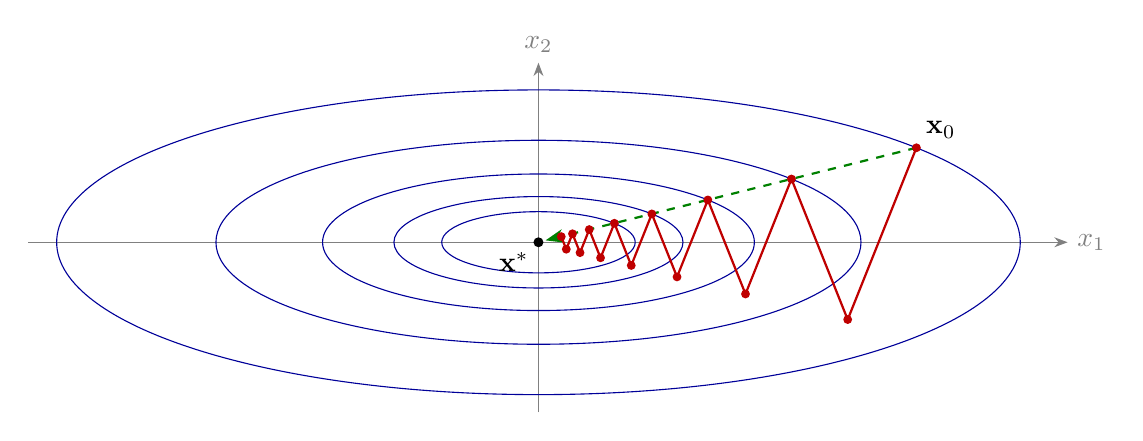
\begin{tikzpicture}[x=0.6cm, y=0.6cm, >=Stealth]
        \draw[->, gray] (-10.8,0) -- (11.2,0) node[right] {$x_1$};
        \draw[->, gray] (0,-3.6) -- (0,3.8) node[above] {$x_2$};
        \foreach \c in {52, 23.3025, 10.4424, 4.6795, 2.0970}
            \draw[blue!60!black] (0,0) ellipse ({sqrt(2*\c)} and {sqrt(2*\c/10)});
        \draw[dashed, ->, thick, green!50!black] (8,2) -- (0.15,0.04);
        \draw[red!75!black, thick] plot coordinates {(8.000,2.000) (6.545,-1.636) (5.355,1.339) (4.382,-1.095) (3.585,0.896) (2.933,-0.733) (2.400,0.600) (1.964,-0.491) (1.607,0.402) (1.314,-0.329) (1.075,0.269) (0.880,-0.220) (0.720,0.180) (0.589,-0.147) (0.482,0.120)};
        \foreach \p in {(8.000,2.000), (6.545,-1.636), (5.355,1.339), (4.382,-1.095), (3.585,0.896), (2.933,-0.733), (2.400,0.600), (1.964,-0.491), (1.607,0.402), (1.314,-0.329), (1.075,0.269), (0.880,-0.220), (0.720,0.180), (0.589,-0.147), (0.482,0.120)}
            \fill[red!75!black] \p circle (1.6pt);
        \node[above right] at (8,2) {$\mathbf{x}_0$};
        \fill (0,0) circle (1.8pt) node[below left] {$\mathbf{x}^*$};
    \end{tikzpicture}
    \caption{Gradient descent on $f(\mathbf{x}) = \frac{1}{2}(x_1^2 + 10x_2^2)$ with the optimal step size $\eta = \frac{2}{11}$, starting at $\mathbf{x}_0 = (8, 2)^\top$ (red: the first $14$ steps). The ellipses are level curves of $f$. Since the condition number is $\kappa = 10$, the level curves are elongated, the gradient points mostly across the valley instead of towards the minimum, and the iterates zig-zag. Newton's method (dashed, Section~\ref{L3-sec:newton}) reaches the minimum in one step.}
    \label{L3-fig:gd}
\end{figure}

For large $\kappa$, the rate $\frac{\kappa - 1}{\kappa + 1} \approx 1 - \frac{2}{\kappa}$ is close to $1$, and the number of steps needed for a given accuracy grows proportionally to $\kappa$. Ill-conditioned problems, whose level sets are long and thin ellipsoids, are slow for gradient descent. This is the zig-zagging that was mentioned at the end of the section on the spectral theorem in Lecture~2.

\begin{remark}[Making gradient descent faster]
    \begin{enumerate}
        \item Feature scaling. For least squares, the Hessian is $2\Phi^\top\Phi$. If the features (the columns of $\Phi$) are measured on very different scales, then $\kappa$ is large. Standardizing each feature, i.e., subtracting its mean and dividing by its standard deviation, often reduces $\kappa$ dramatically.
        \item Momentum. The heavy ball method $\mathbf{x}_{k+1} = \mathbf{x}_k - \eta\nabla f(\mathbf{x}_k) + \beta(\mathbf{x}_k - \mathbf{x}_{k-1})$ keeps some of the previous step. This damps the zig-zagging and accelerates the motion along the valley. For quadratic functions, with well-chosen $\eta$ and $\beta$, the error decreases roughly like $\big(\frac{\sqrt{\kappa} - 1}{\sqrt{\kappa} + 1}\big)^k$, so the number of steps grows only like $\sqrt{\kappa}$.
        \item Preconditioning. Gradient descent with respect to a different inner product $\ip{\mathbf{x}}{\mathbf{y}}_P = \mathbf{x}^\top P\mathbf{y}$ uses the step $-\eta P^{-1}\nabla f(\mathbf{x})$ (Remark~\ref{L3-rem:riesz}), which is the same as gradient descent after a linear change of variables. A good choice of $P$ makes the level sets rounder. Optimizers such as Adam use a diagonal matrix $P$ that is adapted during training. The extreme case $P = \nabla^2 f(\mathbf{x})$ is Newton's method.
    \end{enumerate}
\end{remark}

\begin{remark}[Stochastic gradient descent]\label{L3-rem:sgd}
    In machine learning, the loss is an average over the training data, $L(\boldsymbol{\theta}) = \frac{1}{N}\sum_{i=1}^N \ell_i(\boldsymbol{\theta})$, where $\ell_i$ is the loss on the $i$-th data point. Computing the full gradient needs a pass over all $N$ data points, which is expensive for large data sets. Stochastic gradient descent (SGD) instead chooses a small random subset $B \subseteq \{1, \ldots, N\}$ (a mini-batch) in every step and uses the mini-batch gradient
    \[\mathbf{g} = \frac{1}{|B|}\sum_{i \in B} \nabla\ell_i(\boldsymbol{\theta}),\]
    which is cheap to compute. If $B$ is chosen uniformly at random, then the expected value of $\mathbf{g}$ is the full gradient $\nabla L(\boldsymbol{\theta})$, so on average SGD moves in the right direction. The noise in $\mathbf{g}$ means that SGD does not settle exactly at a minimum unless the step size is decreased during training. In practice, SGD and its variants with momentum and preconditioning are used to train almost all neural networks.
\end{remark}

\subsection{Newton's method}\label{L3-sec:newton}

Gradient descent only uses the first-order approximation of $f$. Newton's method uses the second-order approximation: at $\mathbf{x}_k$, it minimizes the quadratic model
\[m_k(\mathbf{h}) = f(\mathbf{x}_k) + \nabla f(\mathbf{x}_k)^\top\mathbf{h} + \tfrac{1}{2}\mathbf{h}^\top\nabla^2 f(\mathbf{x}_k)\mathbf{h}\]
of Theorem~\ref{L3-thm:taylor2}. If the Hessian $H_k = \nabla^2 f(\mathbf{x}_k)$ is positive definite, then by Example~\ref{L3-ex:quadratic-min} (with $A = H_k$ and $\mathbf{b} = -\nabla f(\mathbf{x}_k)$), the minimum of $m_k$ is $\mathbf{h} = -H_k^{-1}\nabla f(\mathbf{x}_k)$. This gives Newton's method:
\[\mathbf{x}_{k+1} = \mathbf{x}_k - \nabla^2 f(\mathbf{x}_k)^{-1}\nabla f(\mathbf{x}_k).\]
In practice, we do not invert the Hessian, but solve the linear system $H_k\mathbf{h} = -\nabla f(\mathbf{x}_k)$ (Lecture~1). For $n = 1$, Newton's method is $x_{k+1} = x_k - \frac{f'(x_k)}{f''(x_k)}$, i.e., Newton's method for finding a zero of $f'$.
\begin{itemize}
    \item If $f$ is a quadratic function with a positive definite matrix $A$, then $m_0 = f$, and Newton's method finds the minimum in a single step, no matter how large the condition number is (Figure~\ref{L3-fig:gd}).
    \item Near a strict local minimum $\mathbf{x}^*$ with a positive definite Hessian, Newton's method converges quadratically: roughly, the error is squared in every step, $\norm{\mathbf{x}_{k+1} - \mathbf{x}^*} \leq C\norm{\mathbf{x}_k - \mathbf{x}^*}^2$, so the number of correct digits doubles in every step. We do not prove this.
\end{itemize}

\begin{example}\label{L3-ex:newton}
    Let $f(x) = e^x - 2x$. Then $f'(x) = e^x - 2$ and $f''(x) = e^x > 0$, so the minimum is at $x^* = \log 2 = 0.693147\ldots$, and Newton's method is $x_{k+1} = x_k - \frac{e^{x_k} - 2}{e^{x_k}} = x_k - 1 + 2e^{-x_k}$. Starting at $x_0 = 0$:
    \begin{center}
        \renewcommand{\arraystretch}{1.2}
        \begin{tabular}{c|cccccc}
            $k$ & $0$ & $1$ & $2$ & $3$ & $4$ & $5$ \\
            \hline
            $x_k$ & $0$ & $1$ & $0.735759$ & $0.694042$ & $0.6931476$ & $0.693147180560$ \\
            $|x_k - x^*|$ & $0.69$ & $0.31$ & $4.3 \cdot 10^{-2}$ & $9.0 \cdot 10^{-4}$ & $4.0 \cdot 10^{-7}$ & $8.0 \cdot 10^{-14}$
        \end{tabular}
    \end{center}
    Once the iterates are close to $x^*$, the exponent of the error roughly doubles in every step.
\end{example}

Newton's method has two drawbacks. First, for $n$ parameters, the Hessian has $n^2$ entries, and solving the linear system costs about $n^3$ operations, which is impossible for neural networks with millions of parameters. Second, far from a minimum, the Hessian need not be positive definite, and Newton's method can move to a saddle point or a maximum, since it only looks for a critical point. Quasi-Newton methods such as BFGS and L-BFGS build approximations of the Hessian (or of its inverse) from the gradients of previous steps, and are popular for problems with up to a few thousand parameters. Note also that the Newton step $-H_k^{-1}\nabla f(\mathbf{x}_k)$ is the gradient step with respect to the inner product $\ip{\mathbf{x}}{\mathbf{y}}_{H_k} = \mathbf{x}^\top H_k\mathbf{y}$ defined by the Hessian (Remark~\ref{L3-rem:riesz}): Newton's method measures distances in a way that makes the level sets of the quadratic model round.

\section{Convexity}\label{L3-sec:convexity}

Gradient descent and Newton's method only find critical points, and a critical point need not be a global minimum. For an important class of functions, the convex functions, this problem disappears.

\begin{definition}[Convex sets and functions]\label{L3-def:convex}
    A set $C \subseteq \mathbb{R}^n$ is convex if for all $\mathbf{x}, \mathbf{y} \in C$ and all $\theta \in [0, 1]$, also $\theta\mathbf{x} + (1 - \theta)\mathbf{y} \in C$: with any two points, $C$ contains the line segment between them. A function $f: C \to \mathbb{R}$ on a convex set $C$ is convex if
    \[f(\theta\mathbf{x} + (1 - \theta)\mathbf{y}) \leq \theta f(\mathbf{x}) + (1 - \theta)f(\mathbf{y}) \qquad \text{for all } \mathbf{x}, \mathbf{y} \in C, \, \theta \in [0, 1],\]
    and strictly convex if the inequality is strict whenever $\mathbf{x} \neq \mathbf{y}$ and $0 < \theta < 1$. A function $f$ is concave if $-f$ is convex.
\end{definition}

Geometrically, $f$ is convex if the line segment between any two points of its graph lies above the graph (Figure~\ref{L3-fig:convex}). Examples of convex sets are $\mathbb{R}^n$, subspaces, affine subspaces, half-spaces $\{\mathbf{x} : \mathbf{w}^\top\mathbf{x} \leq c\}$, balls $\{\mathbf{x} : \norm{\mathbf{x} - \mathbf{a}} \leq r\}$ for any norm, and intersections of convex sets. A circle is not convex.

\begin{example}\label{L3-ex:convex-functions}
    \begin{enumerate}
        \item Affine functions $f(\mathbf{x}) = \mathbf{a}^\top\mathbf{x} + b$ are convex (and concave), with equality in the definition.
        \item Every norm is convex: by the triangle inequality and homogeneity, $\norm{\theta\mathbf{x} + (1 - \theta)\mathbf{y}} \leq \theta\norm{\mathbf{x}} + (1 - \theta)\norm{\mathbf{y}}$ for $\theta \in [0, 1]$.
        \item The functions $x^2$, $|x|$, $e^x$ on $\mathbb{R}$, and $-\log x$ on $(0, \infty)$ are convex. The function $x^3$ is not convex on $\mathbb{R}$.
    \end{enumerate}
\end{example}

\begin{figure}[ht]
    \centering
    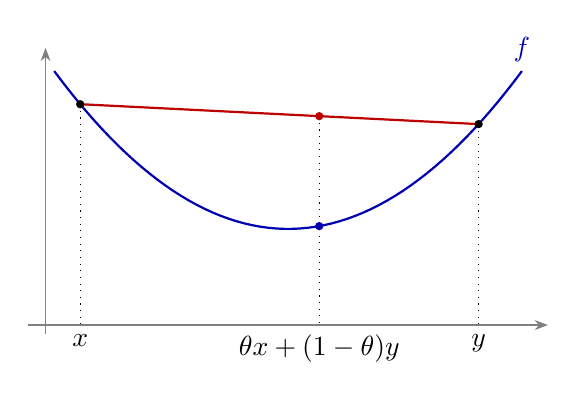
\begin{tikzpicture}[x=1.1cm, y=1.1cm, >=Stealth]
        \draw[->, gray] (-2.4,0) -- (3.6,0);
        \draw[->, gray] (-2.2,-0.1) -- (-2.2,3.2);
        \draw[thick, blue!70!black, domain=-2.1:3.3, samples=60] plot (\x, {0.25*(\x)^2 - 0.3*\x + 1.2});
        \draw[red!75!black, thick] (-1.8,2.55) -- (2.8,2.32);
        \fill (-1.8,2.55) circle (1.5pt);
        \fill (2.8,2.32) circle (1.5pt);
        \draw[dotted] (-1.8,2.55) -- (-1.8,0) node[below] {$x$};
        \draw[dotted] (2.8,2.32) -- (2.8,0) node[below] {$y$};
        \draw[dotted] (0.96,2.412) -- (0.96,0) node[below] {$\theta x + (1 - \theta)y$};
        \fill[red!75!black] (0.96,2.412) circle (1.5pt);
        \fill[blue!70!black] (0.96,1.1424) circle (1.5pt);
        \node[blue!70!black, above] at (3.3,2.93) {$f$};
    \end{tikzpicture}
    \qquad
    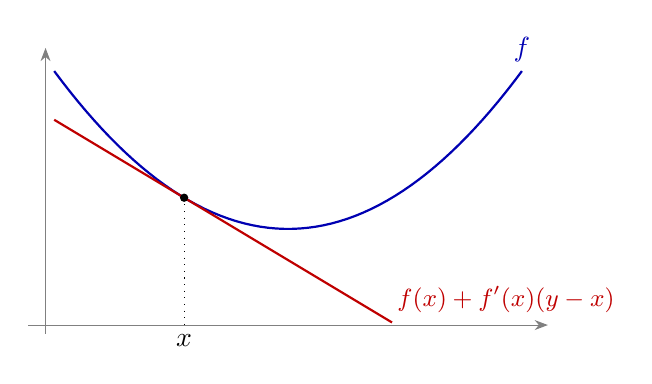
\begin{tikzpicture}[x=1.1cm, y=1.1cm, >=Stealth]
        \draw[->, gray] (-2.4,0) -- (3.6,0);
        \draw[->, gray] (-2.2,-0.1) -- (-2.2,3.2);
        \draw[thick, blue!70!black, domain=-2.1:3.3, samples=60] plot (\x, {0.25*(\x)^2 - 0.3*\x + 1.2});
        \draw[red!75!black, thick, domain=-2.1:1.8] plot (\x, {1.47 - 0.6*(\x + 0.6)});
        \fill (-0.6,1.47) circle (1.5pt);
        \draw[dotted] (-0.6,1.47) -- (-0.6,0) node[below] {$x$};
        \node[red!75!black, font=\small, above right] at (1.75,0.03) {$f(x) + f'(x)(y - x)$};
        \node[blue!70!black, above] at (3.3,2.93) {$f$};
    \end{tikzpicture}
    \caption{Left: a convex function lies below every chord, i.e., $f(\theta x + (1 - \theta)y) \leq \theta f(x) + (1 - \theta)f(y)$. Right: a differentiable convex function lies above every tangent line (Theorem~\ref{L3-thm:convex-first-order}).}
    \label{L3-fig:convex}
\end{figure}

\begin{theorem}[First-order characterization]\label{L3-thm:convex-first-order}
    Let $C \subseteq \mathbb{R}^n$ be open and convex, and let $f: C \to \mathbb{R}$ be differentiable. Then $f$ is convex if and only if
    \[f(\mathbf{y}) \geq f(\mathbf{x}) + \nabla f(\mathbf{x})^\top(\mathbf{y} - \mathbf{x}) \qquad \text{for all } \mathbf{x}, \mathbf{y} \in C.\]
\end{theorem}

\begin{proof}
    Suppose that $f$ is convex, and let $\mathbf{x}, \mathbf{y} \in C$. For $0 < t \leq 1$, convexity with $\theta = 1 - t$ gives $f(\mathbf{x} + t(\mathbf{y} - \mathbf{x})) \leq f(\mathbf{x}) + t\big(f(\mathbf{y}) - f(\mathbf{x})\big)$, so
    \[\frac{f(\mathbf{x} + t(\mathbf{y} - \mathbf{x})) - f(\mathbf{x})}{t} \leq f(\mathbf{y}) - f(\mathbf{x}).\]
    As $t \to 0$, the left side tends to the directional derivative $\nabla f(\mathbf{x})^\top(\mathbf{y} - \mathbf{x})$ (Proposition~\ref{L3-prop:differentiable}).

    Conversely, suppose that the inequality holds, let $\theta \in [0, 1]$, and let $\mathbf{z} = \theta\mathbf{x} + (1 - \theta)\mathbf{y}$. Then $f(\mathbf{x}) \geq f(\mathbf{z}) + \nabla f(\mathbf{z})^\top(\mathbf{x} - \mathbf{z})$ and $f(\mathbf{y}) \geq f(\mathbf{z}) + \nabla f(\mathbf{z})^\top(\mathbf{y} - \mathbf{z})$. Multiplying the first inequality by $\theta$ and the second by $1 - \theta$ and adding, we get
    \[\theta f(\mathbf{x}) + (1 - \theta)f(\mathbf{y}) \geq f(\mathbf{z}) + \nabla f(\mathbf{z})^\top\big(\theta\mathbf{x} + (1 - \theta)\mathbf{y} - \mathbf{z}\big) = f(\mathbf{z}).\qedhere\]
\end{proof}

So the linear approximation of a convex function is a global lower bound. This has a remarkable consequence.

\begin{corollary}\label{L3-cor:convex-global}
    Let $f$ be convex and differentiable on an open convex set $C$. If $\nabla f(\mathbf{x}^*) = \mathbf{0}$, then $\mathbf{x}^*$ is a global minimum of $f$.
\end{corollary}

\begin{proof}
    By Theorem~\ref{L3-thm:convex-first-order}, $f(\mathbf{y}) \geq f(\mathbf{x}^*) + \mathbf{0}^\top(\mathbf{y} - \mathbf{x}^*) = f(\mathbf{x}^*)$ for all $\mathbf{y} \in C$.
\end{proof}

\begin{proposition}\label{L3-prop:convex-minima}
    Let $f: C \to \mathbb{R}$ be convex. Then every local minimum of $f$ is a global minimum, and the set of global minima is convex. If $f$ is strictly convex, it has at most one global minimum.
\end{proposition}

\begin{proof}
    Let $\mathbf{x}^*$ be a local minimum, and suppose that $f(\mathbf{y}) < f(\mathbf{x}^*)$ for some $\mathbf{y} \in C$. For $0 < t \leq 1$, the point $\mathbf{x}_t = (1 - t)\mathbf{x}^* + t\mathbf{y}$ satisfies $f(\mathbf{x}_t) \leq (1 - t)f(\mathbf{x}^*) + tf(\mathbf{y}) < f(\mathbf{x}^*)$, and $\mathbf{x}_t$ is arbitrarily close to $\mathbf{x}^*$ for small $t$. This contradicts the local minimality of $\mathbf{x}^*$. If $\mathbf{x}$ and $\mathbf{y}$ are global minima with $f(\mathbf{x}) = f(\mathbf{y}) = m$, then $f(\theta\mathbf{x} + (1 - \theta)\mathbf{y}) \leq m$, so all points of the segment are global minima. For strictly convex $f$ and $\mathbf{x} \neq \mathbf{y}$, we would get $f(\frac{1}{2}\mathbf{x} + \frac{1}{2}\mathbf{y}) < m$, which is impossible.
\end{proof}

So for convex functions, there are no bad local minima and no saddle points: every critical point is a global minimum, and gradient descent with a suitable step size converges to the minimum value. (One can show that for a convex $L$-smooth function with a minimum $\mathbf{x}^*$, gradient descent with $\eta = \frac{1}{L}$ satisfies $f(\mathbf{x}_k) - f(\mathbf{x}^*) \leq \frac{L\norm{\mathbf{x}_0 - \mathbf{x}^*}^2}{2k}$.) For twice differentiable functions, convexity can be checked with the Hessian.

\begin{theorem}[Second-order characterization]\label{L3-thm:convex-second-order}
    Let $C \subseteq \mathbb{R}^n$ be open and convex, and let $f: C \to \mathbb{R}$ be twice continuously differentiable. Then $f$ is convex if and only if $\nabla^2 f(\mathbf{x})$ is positive semidefinite for all $\mathbf{x} \in C$. If $\nabla^2 f(\mathbf{x})$ is positive definite for all $\mathbf{x} \in C$, then $f$ is strictly convex.
\end{theorem}

\begin{proof}
    If all Hessians are positive semidefinite, then by Theorem~\ref{L3-thm:taylor2}, for all $\mathbf{x}, \mathbf{y} \in C$,
    \[f(\mathbf{y}) = f(\mathbf{x}) + \nabla f(\mathbf{x})^\top(\mathbf{y} - \mathbf{x}) + \tfrac{1}{2}(\mathbf{y} - \mathbf{x})^\top\nabla^2 f(\mathbf{z})(\mathbf{y} - \mathbf{x}) \geq f(\mathbf{x}) + \nabla f(\mathbf{x})^\top(\mathbf{y} - \mathbf{x}),\]
    where $\mathbf{z}$ is a point on the segment between $\mathbf{x}$ and $\mathbf{y}$, so $f$ is convex by Theorem~\ref{L3-thm:convex-first-order}. (If all Hessians are positive definite, the inequality is strict for $\mathbf{y} \neq \mathbf{x}$, and the proof of Theorem~\ref{L3-thm:convex-first-order} then gives strict convexity.) Conversely, suppose that $\mathbf{v}^\top\nabla^2 f(\mathbf{x})\mathbf{v} < 0$ for some $\mathbf{x} \in C$ and $\mathbf{v}$. By the second form of Theorem~\ref{L3-thm:taylor2}, for small $t \neq 0$,
    \[f(\mathbf{x} + t\mathbf{v}) = f(\mathbf{x}) + t\nabla f(\mathbf{x})^\top\mathbf{v} + \tfrac{1}{2}t^2\mathbf{v}^\top\nabla^2 f(\mathbf{x})\mathbf{v} + o(t^2) < f(\mathbf{x}) + \nabla f(\mathbf{x})^\top(t\mathbf{v}),\]
    which contradicts the inequality of Theorem~\ref{L3-thm:convex-first-order} for $\mathbf{y} = \mathbf{x} + t\mathbf{v}$.
\end{proof}

\begin{example}[Convex loss functions]\label{L3-ex:convex-losses}
    \begin{enumerate}
        \item The least squares loss $\norm{\mathbf{y} - \Phi\boldsymbol{\theta}}^2$ has the Hessian $2\Phi^\top\Phi$, which is positive semidefinite, since $\mathbf{v}^\top\Phi^\top\Phi\mathbf{v} = \norm{\Phi\mathbf{v}}^2 \geq 0$. So it is convex, and strictly convex if $\Phi$ has linearly independent columns. Adding a ridge penalty $\lambda\norm{\boldsymbol{\theta}}^2$ with $\lambda > 0$ adds $2\lambda I$ to the Hessian, which makes it positive definite, so ridge regression always has a unique minimum.
        \item The logistic regression loss has the Hessian $\frac{1}{N}\sum_i p_i(1 - p_i)\mathbf{x}_i\mathbf{x}_i^\top$ (Example~\ref{L3-ex:ml-hessians}). It is positive semidefinite, since $\mathbf{v}^\top\mathbf{x}_i\mathbf{x}_i^\top\mathbf{v} = (\mathbf{x}_i^\top\mathbf{v})^2 \geq 0$ and $p_i(1 - p_i) > 0$. So the loss is convex, and every critical point is a global minimum.
        \item The log-sum-exp function has the Hessian $\diag(\mathbf{p}) - \mathbf{p}\mathbf{p}^\top$, where $\mathbf{p}$ has positive entries with sum $1$. For every $\mathbf{v}$, by the Cauchy--Schwarz inequality applied to the vectors with entries $\sqrt{p_i}$ and $\sqrt{p_i}v_i$,
        \[\Big(\sum_i p_i v_i\Big)^2 \leq \Big(\sum_i p_i\Big)\Big(\sum_i p_i v_i^2\Big) = \sum_i p_i v_i^2,\]
        so $\mathbf{v}^\top\big(\diag(\mathbf{p}) - \mathbf{p}\mathbf{p}^\top\big)\mathbf{v} = \sum_i p_i v_i^2 - \big(\sum_i p_i v_i\big)^2 \geq 0$.
        So log-sum-exp is convex, and hence so is the softmax cross-entropy loss of Example~\ref{L3-ex:softmax-ce}.
    \end{enumerate}
\end{example}

\begin{proposition}[Operations that preserve convexity]\label{L3-prop:convex-operations}
    \begin{enumerate}
        \item If $f$ and $g$ are convex and $\alpha, \beta \geq 0$, then $\alpha f + \beta g$ is convex.
        \item If $f$ is convex, then $\mathbf{x} \mapsto f(A\mathbf{x} + \mathbf{b})$ is convex.
        \item If $f$ and $g$ are convex, then $\mathbf{x} \mapsto \max(f(\mathbf{x}), g(\mathbf{x}))$ is convex.
    \end{enumerate}
\end{proposition}

\begin{proof}
    (1) Add the inequalities for $f$ and $g$, multiplied by $\alpha$ and $\beta$. (2) The map $\mathbf{x} \mapsto A\mathbf{x} + \mathbf{b}$ maps $\theta\mathbf{x} + (1 - \theta)\mathbf{y}$ to $\theta(A\mathbf{x} + \mathbf{b}) + (1 - \theta)(A\mathbf{y} + \mathbf{b})$; now use the convexity of $f$. (3) $f(\theta\mathbf{x} + (1 - \theta)\mathbf{y}) \leq \theta f(\mathbf{x}) + (1 - \theta)f(\mathbf{y}) \leq \theta\max(f, g)(\mathbf{x}) + (1 - \theta)\max(f, g)(\mathbf{y})$, and similarly for $g$.
\end{proof}

For example, the hinge loss $\max(0, 1 - y\,\mathbf{w}^\top\mathbf{x})$ of support vector machines is convex in $\mathbf{w}$, as the maximum of two affine functions, and so are the $\ell_1$ and $\ell_2$ regularization terms $\lambda\norm{\mathbf{w}}_1$ and $\lambda\norm{\mathbf{w}}^2$.

\begin{remark}[Neural networks are not convex]
    The loss of a neural network with a hidden layer is not convex as a function of the weights. One reason is symmetry: if we swap two hidden units, i.e., swap two rows of $W_1$, the corresponding entries of $\mathbf{b}_1$, and the corresponding columns of $W_2$, the network computes the same function, so the loss does not change. If $\boldsymbol{\theta}^*$ is a global minimum, then so is the swapped parameter vector $\boldsymbol{\theta}'$. If the loss were convex, then by Proposition~\ref{L3-prop:convex-minima} the midpoint $\frac{1}{2}(\boldsymbol{\theta}^* + \boldsymbol{\theta}')$ would be a global minimum too. But in the midpoint, the two hidden units have identical weights, so the network effectively has one hidden unit less, and its loss is usually larger. Nevertheless, gradient-based methods work remarkably well for neural networks in practice, which is an active area of research.
\end{remark}

\section{Constrained Optimization}\label{L3-sec:constrained}

Many optimization problems in machine learning have constraints. In principal component analysis, we maximize the variance over unit vectors; a vector of probabilities must have nonnegative entries that sum to $1$; and support vector machines maximize a margin subject to classifying all training points correctly. We first consider equality constraints:
\[\text{minimize } f(\mathbf{x}) \quad \text{subject to} \quad g_1(\mathbf{x}) = 0, \ \ldots, \ g_m(\mathbf{x}) = 0.\]

\subsection{Lagrange multipliers}

Consider first one constraint $g(\mathbf{x}) = 0$ in $\mathbb{R}^2$, which is usually a curve. If we walk along the curve, then at a local minimum of $f$ on the curve, the derivative of $f$ in the direction of the curve must be zero, i.e., $\nabla f(\mathbf{x}^*)$ is orthogonal to the curve. By Corollary~\ref{L3-cor:level-sets}, $\nabla g(\mathbf{x}^*)$ is also orthogonal to the curve, which is a level set of $g$. In the plane, this means that $\nabla f(\mathbf{x}^*)$ and $\nabla g(\mathbf{x}^*)$ are parallel: the level curve of $f$ through $\mathbf{x}^*$ touches the constraint curve (Figure~\ref{L3-fig:lagrange}). At a point where $\nabla f$ is not orthogonal to the curve, we can decrease $f$ by moving along the curve.

\begin{theorem}[Lagrange multipliers]\label{L3-thm:lagrange}
    Let $f, g_1, \ldots, g_m: D \to \mathbb{R}$ be continuously differentiable on an open set $D \subseteq \mathbb{R}^n$, and let $\mathbf{x}^*$ be a local minimum of $f$ on the set $S = \{\mathbf{x} \in D : g_1(\mathbf{x}) = \cdots = g_m(\mathbf{x}) = 0\}$. If the gradients $\nabla g_1(\mathbf{x}^*), \ldots, \nabla g_m(\mathbf{x}^*)$ are linearly independent, then there are unique numbers $\lambda_1, \ldots, \lambda_m \in \mathbb{R}$, called Lagrange multipliers, such that
    \[\nabla f(\mathbf{x}^*) + \lambda_1\nabla g_1(\mathbf{x}^*) + \cdots + \lambda_m\nabla g_m(\mathbf{x}^*) = \mathbf{0}.\]
\end{theorem}

\begin{proof}[Sketch of proof]
    Let $U = \Span\{\nabla g_1(\mathbf{x}^*), \ldots, \nabla g_m(\mathbf{x}^*)\}$. If $\mathbf{x}(t)$ is a differentiable curve in $S$ with $\mathbf{x}(0) = \mathbf{x}^*$, then $g_i(\mathbf{x}(t)) = 0$ for all $t$, so $\nabla g_i(\mathbf{x}^*)^\top\mathbf{x}'(0) = 0$ by the chain rule, i.e., the tangent vector $\mathbf{x}'(0)$ lies in $U^\perp$. Conversely, the implicit function theorem from analysis, which we do not prove, shows that, since the $\nabla g_i(\mathbf{x}^*)$ are linearly independent, every vector $\mathbf{v} \in U^\perp$ is the tangent vector $\mathbf{x}'(0)$ of such a curve. Since $t \mapsto f(\mathbf{x}(t))$ has a local minimum at $t = 0$, its derivative $\nabla f(\mathbf{x}^*)^\top\mathbf{x}'(0)$ is $0$. Hence $\nabla f(\mathbf{x}^*)$ is orthogonal to every vector in $U^\perp$, i.e., $\nabla f(\mathbf{x}^*) \in (U^\perp)^\perp = U$ (Lecture~2). So $\nabla f(\mathbf{x}^*)$ is a linear combination of the $\nabla g_i(\mathbf{x}^*)$, and the coefficients are unique, since the $\nabla g_i(\mathbf{x}^*)$ are linearly independent.
\end{proof}

The same condition holds at local maxima (apply the theorem to $-f$; the multipliers can have any sign). It is convenient to write it with the Lagrangian
\[\mathcal{L}(\mathbf{x}, \boldsymbol{\lambda}) = f(\mathbf{x}) + \lambda_1 g_1(\mathbf{x}) + \cdots + \lambda_m g_m(\mathbf{x}).\]
The condition of the theorem says that $\nabla_{\mathbf{x}}\mathcal{L}(\mathbf{x}^*, \boldsymbol{\lambda}) = \mathbf{0}$, and the constraints say that $\nabla_{\boldsymbol{\lambda}}\mathcal{L}(\mathbf{x}^*, \boldsymbol{\lambda}) = (g_1(\mathbf{x}^*), \ldots, g_m(\mathbf{x}^*))^\top = \mathbf{0}$. So we look for critical points of $\mathcal{L}$, which gives $n + m$ equations for the $n + m$ unknowns $\mathbf{x}$ and $\boldsymbol{\lambda}$. If $S$ is closed and bounded (such as a sphere), then $f$ attains its minimum and maximum on $S$ (this is a theorem from analysis), and we find them by comparing the values of $f$ at all solutions of these equations.

\begin{example}\label{L3-ex:lagrange-circle}
    We find the maximum and minimum of $f(x, y) = x + y$ on the unit circle $g(x, y) = x^2 + y^2 - 1 = 0$. The condition $\nabla f + \lambda\nabla g = \mathbf{0}$ is $(1, 1) + \lambda(2x, 2y) = (0, 0)$, so $x = y = -\frac{1}{2\lambda}$, and with $x^2 + y^2 = 1$, we get $x = y = \pm\frac{1}{\sqrt{2}}$. The maximum is $f(\frac{1}{\sqrt{2}}, \frac{1}{\sqrt{2}}) = \sqrt{2}$, and the minimum is $-\sqrt{2}$. This agrees with the Cauchy--Schwarz inequality: $x + y = (1, 1)(x, y)^\top \leq \sqrt{2}\sqrt{x^2 + y^2} = \sqrt{2}$. See Figure~\ref{L3-fig:lagrange}.
\end{example}

\begin{figure}[ht]
    \centering
    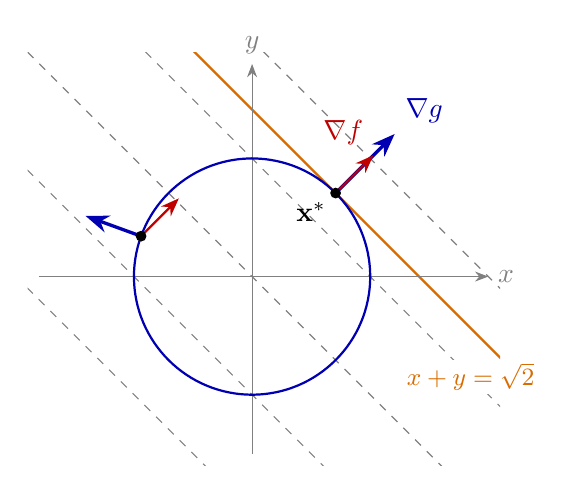
\begin{tikzpicture}[scale=1.5, >=Stealth]
        \begin{scope}
            \clip (-1.9,-1.6) rectangle (2.1,1.9);
            \foreach \c in {-2,-1,0,1,2}
                \draw[gray, dashed] ({\c/2 - 2},{\c/2 + 2}) -- ({\c/2 + 2},{\c/2 - 2});
            \draw[orange!85!black, thick] ({sqrt(2)/2 - 2},{sqrt(2)/2 + 2}) -- ({sqrt(2)/2 + 2},{sqrt(2)/2 - 2});
        \end{scope}
        \draw[->, gray] (-1.8,0) -- (2.0,0) node[right] {$x$};
        \draw[->, gray] (0,-1.5) -- (0,1.8) node[above] {$y$};
        \draw[blue!70!black, thick] (0,0) circle (1);
        \coordinate (P) at (45:1);
        \draw[->, very thick, blue!70!black] (P) -- ++(0.5,0.5) node[above right] {$\nabla g$};
        \draw[->, thick, red!75!black] (P) -- ++(0.32,0.32) node[above left] {$\nabla f$};
        \fill (P) circle (1.3pt) node[below left] {$\mathbf{x}^*$};
        \coordinate (Q) at (160:1);
        \draw[->, thick, red!75!black] (Q) -- ++(0.32,0.32);
        \draw[->, very thick, blue!70!black] (Q) -- ++({0.5*cos(160)},{0.5*sin(160)});
        \fill (Q) circle (1.3pt);
        \node[orange!85!black, font=\small, fill=white, inner sep=1pt] at (1.85,-0.85) {$x + y = \sqrt{2}$};
    \end{tikzpicture}
    \caption{Maximizing $f(x, y) = x + y$ on the unit circle $g(x, y) = x^2 + y^2 - 1 = 0$. The dashed lines are level lines of $f$. At the maximum $\mathbf{x}^*$, the level line $x + y = \sqrt{2}$ touches the circle, and $\nabla f$ and $\nabla g$ are parallel. At the other marked point, they are not parallel: $\nabla f$ has a component along the circle, so moving along the circle in that direction increases $f$.}
    \label{L3-fig:lagrange}
\end{figure}

\begin{example}[Eigenvalues and PCA]\label{L3-ex:lagrange-eigen}
    Let $A$ be a symmetric $n \times n$ matrix. We maximize $f(\mathbf{x}) = \mathbf{x}^\top A\mathbf{x}$ subject to $g(\mathbf{x}) = 1 - \mathbf{x}^\top\mathbf{x} = 0$. Here $\nabla g(\mathbf{x}) = -2\mathbf{x} \neq \mathbf{0}$ on the unit sphere, and the Lagrange condition $2A\mathbf{x} - 2\lambda\mathbf{x} = \mathbf{0}$ says that
    \[A\mathbf{x} = \lambda\mathbf{x}:\]
    the candidates are exactly the unit eigenvectors of $A$, and the Lagrange multiplier is the eigenvalue. At a unit eigenvector, $f(\mathbf{x}) = \mathbf{x}^\top(\lambda\mathbf{x}) = \lambda$. Since the sphere is closed and bounded, the maximum exists, and it is the largest eigenvalue $\lambda_{\max}$, attained at a corresponding eigenvector. This is the Rayleigh quotient result of Lecture~2, found with calculus instead of the spectral theorem; in PCA, it gives the first principal component.
\end{example}

\begin{example}[The minimum norm solution]\label{L3-ex:min-norm}
    Let $A \in \mathbb{R}^{m \times n}$ have linearly independent rows $\mathbf{a}_1^\top, \ldots, \mathbf{a}_m^\top$ (so $m \leq n$), and let $\mathbf{b} \in \mathbb{R}^m$. The system $A\mathbf{x} = \mathbf{b}$ has infinitely many solutions if $m < n$, and we look for the one with the smallest norm: minimize $\norm{\mathbf{x}}^2$ subject to $g_i(\mathbf{x}) = \mathbf{a}_i^\top\mathbf{x} - b_i = 0$ for $i = 1, \ldots, m$. The gradients $\nabla g_i = \mathbf{a}_i$ are linearly independent, and the Lagrange condition is
    \[2\mathbf{x} + \sum_{i=1}^m \lambda_i\mathbf{a}_i = 2\mathbf{x} + A^\top\boldsymbol{\lambda} = \mathbf{0}, \qquad \text{so} \qquad \mathbf{x} = A^\top\boldsymbol{\mu} \text{ with } \boldsymbol{\mu} = -\tfrac{1}{2}\boldsymbol{\lambda}.\]
    So $\mathbf{x}$ lies in the row space of $A$. Substituting into $A\mathbf{x} = \mathbf{b}$ gives $AA^\top\boldsymbol{\mu} = \mathbf{b}$. The $m \times m$ matrix $AA^\top$ is invertible (it is positive definite, since $\mathbf{v}^\top AA^\top\mathbf{v} = \norm{A^\top\mathbf{v}}^2 > 0$ for $\mathbf{v} \neq \mathbf{0}$), so
    \[\mathbf{x}^* = A^\top(AA^\top)^{-1}\mathbf{b}.\]
    This is indeed the global minimum: every solution of $A\mathbf{x} = \mathbf{b}$ is $\mathbf{x} = \mathbf{x}^* + \mathbf{v}$ with $\mathbf{v} \in \Null(A)$, and since $\mathbf{x}^* \in \row(A) = \Null(A)^\perp$, Pythagoras gives $\norm{\mathbf{x}}^2 = \norm{\mathbf{x}^*}^2 + \norm{\mathbf{v}}^2 \geq \norm{\mathbf{x}^*}^2$. By the proposition on the pseudo-inverse in Lecture~2, applied to $A^\top$ (which has linearly independent columns), $(A^\top)^+ = (AA^\top)^{-1}A$. By the definition of the pseudo-inverse with the SVD, $(A^\top)^+ = (A^+)^\top$, so taking transposes gives $A^+ = A^\top(AA^\top)^{-1}$. So $\mathbf{x}^* = A^+\mathbf{b}$, which proves, for matrices with linearly independent rows, the claim of Lecture~2 that $A^+\mathbf{b}$ is the solution with the smallest norm.
\end{example}

\subsection{Inequality constraints and the KKT conditions}

Now consider inequality constraints:
\[\text{minimize } f(\mathbf{x}) \quad \text{subject to} \quad g_1(\mathbf{x}) \leq 0, \ \ldots, \ g_m(\mathbf{x}) \leq 0.\]
At a feasible point $\mathbf{x}^*$, the constraint $g_i$ is active if $g_i(\mathbf{x}^*) = 0$, and inactive if $g_i(\mathbf{x}^*) < 0$. Inactive constraints do not matter near $\mathbf{x}^*$, since they remain satisfied when we move $\mathbf{x}^*$ a little. Active constraints behave like equality constraints, with one difference: moving into the feasible region, where $g_i < 0$, is allowed. At a minimum, this must not decrease $f$, and this forces the multipliers to be nonnegative.

\begin{theorem}[Karush--Kuhn--Tucker conditions]\label{L3-thm:kkt}
    Let $f, g_1, \ldots, g_m$ be continuously differentiable, and let $\mathbf{x}^*$ be a local minimum of $f$ subject to $g_1(\mathbf{x}) \leq 0, \ldots, g_m(\mathbf{x}) \leq 0$, such that the gradients of the active constraints at $\mathbf{x}^*$ are linearly independent. Then there are numbers $\mu_1, \ldots, \mu_m$ such that:
    \begin{enumerate}
        \item (stationarity) $\nabla f(\mathbf{x}^*) + \mu_1\nabla g_1(\mathbf{x}^*) + \cdots + \mu_m\nabla g_m(\mathbf{x}^*) = \mathbf{0}$;
        \item (primal feasibility) $g_i(\mathbf{x}^*) \leq 0$ for all $i$;
        \item (dual feasibility) $\mu_i \geq 0$ for all $i$;
        \item (complementary slackness) $\mu_i g_i(\mathbf{x}^*) = 0$ for all $i$, i.e., $\mu_i = 0$ for every inactive constraint.
    \end{enumerate}
    Conversely, if $f$ and all $g_i$ are convex and differentiable, then every $\mathbf{x}^*$ that satisfies (1)--(4) for some $\mu_1, \ldots, \mu_m$ is a global minimum.
\end{theorem}

\begin{proof}[Proof of the converse]
    We do not prove the first part. For the converse, let $\mathbf{x}$ be feasible. The function $\mathcal{L}(\mathbf{z}) = f(\mathbf{z}) + \sum_i \mu_i g_i(\mathbf{z})$ is convex by Proposition~\ref{L3-prop:convex-operations}, since $\mu_i \geq 0$, and $\nabla\mathcal{L}(\mathbf{x}^*) = \mathbf{0}$ by (1). By Corollary~\ref{L3-cor:convex-global}, $\mathcal{L}(\mathbf{x}) \geq \mathcal{L}(\mathbf{x}^*)$. Since $\mu_i g_i(\mathbf{x}) \leq 0$ for feasible $\mathbf{x}$ and $\mu_i g_i(\mathbf{x}^*) = 0$ by (4),
    \[f(\mathbf{x}) \geq f(\mathbf{x}) + \sum_i \mu_i g_i(\mathbf{x}) = \mathcal{L}(\mathbf{x}) \geq \mathcal{L}(\mathbf{x}^*) = f(\mathbf{x}^*).\qedhere\]
\end{proof}

Equality constraints can be added to the KKT conditions with multipliers of any sign, as in Theorem~\ref{L3-thm:lagrange}.

\begin{example}\label{L3-ex:kkt-1d}
    Minimize $f(x) = (x - 2)^2$ subject to $x \leq 1$, i.e., $g(x) = x - 1 \leq 0$. The KKT conditions are $2(x - 2) + \mu = 0$, $x \leq 1$, $\mu \geq 0$ and $\mu(x - 1) = 0$. If $\mu = 0$, then $x = 2$, which is not feasible. So the constraint is active, $x = 1$, and $\mu = 2 \geq 0$. Since $f$ and $g$ are convex, $x^* = 1$ is the global minimum. The multiplier measures how much the constraint costs: if we relax it to $x \leq 1 + \varepsilon$, the minimum value $(1 + \varepsilon - 2)^2 = 1 - 2\varepsilon + \varepsilon^2$ decreases at the rate $\mu = 2$. For the constraint $x \leq 3$ instead, the minimum $x^* = 2$ satisfies the constraint, which is inactive, and $\mu = 0$.
\end{example}

\begin{example}[Projection onto a ball]\label{L3-ex:kkt-ball}
    Let $\mathbf{p} \in \mathbb{R}^n$ with $\norm{\mathbf{p}} > 1$. We find the point of the unit ball closest to $\mathbf{p}$: minimize $\norm{\mathbf{x} - \mathbf{p}}^2$ subject to $\norm{\mathbf{x}}^2 - 1 \leq 0$. Stationarity is $2(\mathbf{x} - \mathbf{p}) + 2\mu\mathbf{x} = \mathbf{0}$, i.e., $\mathbf{x} = \frac{\mathbf{p}}{1 + \mu}$. If $\mu = 0$, then $\mathbf{x} = \mathbf{p}$ is not feasible, so the constraint is active, $\norm{\mathbf{x}} = 1$, which gives $1 + \mu = \norm{\mathbf{p}}$, $\mu = \norm{\mathbf{p}} - 1 > 0$, and
    \[\mathbf{x}^* = \frac{\mathbf{p}}{\norm{\mathbf{p}}}.\]
    For example, for $\mathbf{p} = (3, 4)^\top$, we get $\mathbf{x}^* = (0.6, 0.8)^\top$ and $\mu = 4$. This projection is used in projected gradient descent, which alternates gradient steps with projections onto the feasible set.
\end{example}

\begin{remark}[Support vector machines]
    For linearly separable data $(\mathbf{x}_i, y_i)$ with labels $y_i = \pm 1$, the support vector machine finds the separating hyperplane $\mathbf{w}^\top\mathbf{x} + b = 0$ with the largest margin. By the formula for the distance to a hyperplane in Lecture~2, this leads to the convex problem
    \[\text{minimize } \tfrac{1}{2}\norm{\mathbf{w}}^2 \quad \text{subject to} \quad 1 - y_i(\mathbf{w}^\top\mathbf{x}_i + b) \leq 0 \quad \text{for } i = 1, \ldots, N,\]
    whose margin is $\frac{1}{\norm{\mathbf{w}}}$. The stationarity condition gives $\mathbf{w} = \sum_i \mu_i y_i\mathbf{x}_i$, and by complementary slackness, $\mu_i > 0$ only for the points with $y_i(\mathbf{w}^\top\mathbf{x}_i + b) = 1$, which lie exactly on the margin. These points are the support vectors: the classifier only depends on them.
\end{remark}

\section{Vector Fields: Divergence and Curl}\label{L3-sec:vector-fields}

\begin{definition}[Vector field]\label{L3-def:vector-field}
    A vector field on an open set $D \subseteq \mathbb{R}^n$ is a function $F: D \to \mathbb{R}^n$. We picture it by attaching to every point $\mathbf{x} \in D$ the arrow $F(\mathbf{x})$, starting at $\mathbf{x}$.
\end{definition}

The most important examples for us are gradient fields: the gradient $\nabla f$ of a differentiable function $f: D \to \mathbb{R}$ is a vector field, whose arrows point in the direction of steepest ascent of $f$ and are orthogonal to its level sets (Section~\ref{L3-sec:gradients}). Another example is the velocity field of a fluid, which tells us how fast and in which direction a particle at $\mathbf{x}$ moves. This motion is described by a differential equation, the subject of Lecture~5.

The derivative of a vector field is a square matrix, the Jacobian $DF(\mathbf{x}) \in \mathbb{R}^{n \times n}$, and in this section we extract two geometric quantities from it: the divergence, which measures how much of $F$ flows out of small regions, and the curl, which measures how $F$ rotates.

\begin{example}\label{L3-ex:vector-fields}
    \begin{enumerate}
        \item The gradient field of $f(\mathbf{x}) = \frac{1}{2}\norm{\mathbf{x}}^2$ is $F(\mathbf{x}) = \mathbf{x}$, which points away from the origin. For a symmetric matrix $A$, the field $A\mathbf{x}$ is the gradient field of $\frac{1}{2}\mathbf{x}^\top A\mathbf{x}$ (Proposition~\ref{L3-prop:basic-gradients}).
        \item The rotation field $F(x, y) = (-y, x)^\top$ is orthogonal to the position vector $(x, y)^\top$ everywhere: its arrows go around the origin counterclockwise (Figure~\ref{L3-fig:vector-fields}).
        \item Let $p$ be a positive probability density on $\mathbb{R}^n$. Its score is the vector field $\mathbf{s}(\mathbf{x}) = \nabla\log p(\mathbf{x}) = \frac{\nabla p(\mathbf{x})}{p(\mathbf{x})}$, which points in the direction in which the density increases fastest. For the Gaussian density $p(\mathbf{x}) \propto \exp\big(-\frac{1}{2}(\mathbf{x} - \boldsymbol{\mu})^\top\Sigma^{-1}(\mathbf{x} - \boldsymbol{\mu})\big)$ of Lecture~4, $\mathbf{s}(\mathbf{x}) = -\Sigma^{-1}(\mathbf{x} - \boldsymbol{\mu})$ points towards the mean. Score-based generative models, such as diffusion models, learn the score of the distribution of the training data with a neural network $\mathbf{s}_{\boldsymbol{\theta}}: \mathbb{R}^n \to \mathbb{R}^n$ (Lecture~4).
    \end{enumerate}
\end{example}

Near a point $\mathbf{x}$, $F(\mathbf{x} + \mathbf{h}) \approx F(\mathbf{x}) + DF(\mathbf{x})\mathbf{h}$, and every square matrix is the sum of a symmetric and a skew-symmetric matrix:
\[DF(\mathbf{x}) = S + W, \qquad S = \tfrac{1}{2}\big(DF(\mathbf{x}) + DF(\mathbf{x})^\top\big), \qquad W = \tfrac{1}{2}\big(DF(\mathbf{x}) - DF(\mathbf{x})^\top\big).\]
By the spectral theorem (Lecture~2), $S$ has an orthonormal basis of eigenvectors: the symmetric part stretches or compresses a small neighborhood of $\mathbf{x}$ along these orthogonal directions, at rates given by the eigenvalues. The skew-symmetric part satisfies $\mathbf{h}^\top W\mathbf{h} = 0$, so $W\mathbf{h}$ is orthogonal to $\mathbf{h}$: it is an infinitesimal rotation. The divergence summarizes the symmetric part, and the curl is the skew-symmetric part.

\begin{definition}[Divergence]\label{L3-def:divergence}
    The divergence of a differentiable vector field $F$ is the function
    \[\Div F(\mathbf{x}) = \frac{\partial F_1}{\partial x_1}(\mathbf{x}) + \cdots + \frac{\partial F_n}{\partial x_n}(\mathbf{x}) = \tr DF(\mathbf{x}).\]
    It is also written $\nabla \cdot F$, as a formal dot product of $\nabla = (\frac{\partial}{\partial x_1}, \ldots, \frac{\partial}{\partial x_n})^\top$ with $F$.
\end{definition}

Since $\tr W = 0$, the divergence only depends on the symmetric part: $\Div F(\mathbf{x}) = \tr S$ is the sum of the stretching rates. To see what it measures, think of $F$ as the velocity field of a fluid, and consider a small box $Q$ around $\mathbf{x}$ with the side lengths $h_1, \ldots, h_n$. The two faces of $Q$ perpendicular to $\mathbf{e}_1$ have the area $\frac{\vol(Q)}{h_1}$ and the outward normals $\pm\mathbf{e}_1$, so the fluid flows out through them at the rates $F_1 \cdot \frac{\vol(Q)}{h_1}$ and $-F_1 \cdot \frac{\vol(Q)}{h_1}$, evaluated at the centers of the faces. The net outflow through the two faces is approximately
\[\Big(F_1\big(\mathbf{x} + \tfrac{h_1}{2}\mathbf{e}_1\big) - F_1\big(\mathbf{x} - \tfrac{h_1}{2}\mathbf{e}_1\big)\Big)\frac{\vol(Q)}{h_1} \approx \frac{\partial F_1}{\partial x_1}(\mathbf{x})\vol(Q).\]
Adding the contributions of all $n$ pairs of faces, we find that the net outflow from $Q$ is approximately $\Div F(\mathbf{x})$ times the volume of $Q$. In other words,
\begin{center}
    \emph{$\Div F(\mathbf{x})$ is the net outflow of $F$ per unit volume near $\mathbf{x}$.}
\end{center}
The divergence theorem (Theorem~\ref{L3-thm:divergence}) makes this precise. A vector field with positive divergence at $\mathbf{x}$ acts like a source there, one with negative divergence like a sink, and a field with $\Div F = 0$ describes an incompressible fluid, in which as much flows into every region as flows out. In Lecture~5, we will see that the divergence is also the rate at which the flow of the differential equation $\mathbf{x}' = F(\mathbf{x})$ expands volumes.

\begin{example}\label{L3-ex:divergence}
    \begin{enumerate}
        \item $F(\mathbf{x}) = \mathbf{x}$ has $\Div F = n$: the field points away from the origin and grows in length, so more flows out of every small region than flows in.
        \item The rotation field $(-y, x)^\top$ has $\Div F = 0 + 0 = 0$: the fluid circulates without being compressed.
        \item For $F(\mathbf{x}) = A\mathbf{x}$, we have $DF = A$ and $\Div F = \tr A$. For example, the field of $A = \left(\begin{smallmatrix} -2 & 1 \\ 1 & -2 \end{smallmatrix}\right)$ has $\Div F = -4$ everywhere: it is a sink.
        \item The field $-\nabla f$, which points downhill, has $\Div(-\nabla f) = -\tr\nabla^2 f$. Near a strict local minimum, where the Hessian is positive definite, it is a sink.
    \end{enumerate}
\end{example}

\begin{definition}[Laplacian]\label{L3-def:laplacian}
    The Laplacian of a twice differentiable function $f: D \to \mathbb{R}$ is
    \[\Delta f = \Div\nabla f = \frac{\partial^2 f}{\partial x_1^2} + \cdots + \frac{\partial^2 f}{\partial x_n^2} = \tr\nabla^2 f.\]
    Functions with $\Delta f = 0$ are called harmonic.
\end{definition}

The trace of the Hessian is the sum of its eigenvalues, so $\Delta f(\mathbf{x})$ is the sum of the curvatures of $f$ in the principal directions (Section~\ref{L3-sec:hessian-eigen}), and $\Delta f \geq 0$ at a local minimum. For example, $\Delta\norm{\mathbf{x}}^2 = 2n$, while $x^2 - y^2$ is harmonic: the curvatures $2$ and $-2$ of the saddle cancel. The Laplacian also describes diffusion, such as the spreading of heat, or of the probability density of a randomly moving particle (Lecture~5).

\begin{definition}[Curl]\label{L3-def:curl}
    The curl of a differentiable vector field $F$ on $D \subseteq \mathbb{R}^2$ is the function $\curl F = \frac{\partial F_2}{\partial x_1} - \frac{\partial F_1}{\partial x_2}$. For $D \subseteq \mathbb{R}^3$, it is the vector field
    \[\curl F = \nabla \times F = \Big(\frac{\partial F_3}{\partial x_2} - \frac{\partial F_2}{\partial x_3}, \ \frac{\partial F_1}{\partial x_3} - \frac{\partial F_3}{\partial x_1}, \ \frac{\partial F_2}{\partial x_1} - \frac{\partial F_1}{\partial x_2}\Big)^\top.\]
\end{definition}

Up to the factor $2$, the entries of the curl are the entries $W_{ij} = \frac{1}{2}\big(\frac{\partial F_i}{\partial x_j} - \frac{\partial F_j}{\partial x_i}\big)$ of the skew-symmetric part. For $n = 2$,
\[W = \frac{\curl F(\mathbf{x})}{2}\begin{pmatrix} 0 & -1 \\ 1 & 0 \end{pmatrix},\]
so on top of the stretching by $S$, the field rotates a small neighborhood of $\mathbf{x}$ counterclockwise with the angular velocity $\frac{1}{2}\curl F(\mathbf{x})$: a small paddle wheel in a fluid with the velocity field $F$ spins at this rate. For $n = 3$, one checks that $W\mathbf{h} = \frac{1}{2}\curl F(\mathbf{x}) \times \mathbf{h}$, a rotation about the axis $\curl F(\mathbf{x})$ with the angular velocity $\frac{1}{2}\norm{\curl F(\mathbf{x})}$. In $n$ dimensions, the skew-symmetric matrix $W$ has $\frac{n(n - 1)}{2}$ independent entries, which is $1$ for $n = 2$ and $3$ for $n = 3$; only in three dimensions can they be arranged into a vector field.

\begin{example}\label{L3-ex:curl}
    \begin{enumerate}
        \item The rotation field $(-y, x)^\top$ has $\curl F = 1 - (-1) = 2$, so it rotates with the angular velocity $1$. The field $\mathbf{x}$ has $\curl F = 0$.
        \item The shear field $F(x, y) = (y, 0)^\top$ (Figure~\ref{L3-fig:vector-fields}) has $\Div F = 0$ and $\curl F = -1$. Its Jacobian splits as
        \[\begin{pmatrix} 0 & 1 \\ 0 & 0 \end{pmatrix} = \begin{pmatrix} 0 & \frac{1}{2} \\ \frac{1}{2} & 0 \end{pmatrix} + \begin{pmatrix} 0 & \frac{1}{2} \\ -\frac{1}{2} & 0 \end{pmatrix}:\]
        the shear of Lecture~1 combines a stretching along $(1, 1)$ and a compression along $(1, -1)$ (the eigenvalues $\pm\frac{1}{2}$ of $S$) with a clockwise rotation with the angular velocity $\frac{1}{2}$.
    \end{enumerate}
\end{example}

\begin{figure}[ht]
    \centering
    \newcommand{\fieldpanel}[4]{%
        \begin{scope}[shift={(#1,0)}]
            \draw[gray!60] (-1.3,0) -- (1.3,0) (0,-1.3) -- (0,1.3);
            \foreach \x in {-1,-0.5,...,1}
                \foreach \y in {-1,-0.5,...,1} {
                    \pgfmathsetmacro{\u}{0.3*(#2)}
                    \pgfmathsetmacro{\v}{0.3*(#3)}
                    \pgfmathsetmacro{\len}{abs(\u) + abs(\v)}
                    \ifdim \len pt > 0.001pt
                        \draw[->, thick, blue!70!black] (\x,\y) -- ++(\u,\v);
                    \else
                        \fill[blue!70!black] (\x,\y) circle (0.9pt);
                    \fi
                }
            \node[below, align=center, font=\small] at (0,-1.4) {#4};
        \end{scope}}
    \begin{tikzpicture}[x=1.35cm, y=1.35cm, >=Stealth]
        \fieldpanel{0}{\x}{\y}{source $F = (x, y)$\\ $\Div F = 2$, \ $\curl F = 0$}
        \fieldpanel{3.4}{0-(\y)}{\x}{rotation $F = (-y, x)$\\ $\Div F = 0$, \ $\curl F = 2$}
        \fieldpanel{6.8}{\y}{0}{shear $F = (y, 0)$\\ $\Div F = 0$, \ $\curl F = -1$}
    \end{tikzpicture}
    \caption{Three linear vector fields. The source expands areas and does not rotate, the rotation turns without changing areas, and the shear is a combination of a stretching (along the diagonal) and a clockwise rotation, which preserves areas.}
    \label{L3-fig:vector-fields}
\end{figure}

\begin{proposition}\label{L3-prop:curl-grad}
    Let $f$ and $F$ be twice continuously differentiable.
    \begin{enumerate}
        \item The Jacobian of $\nabla f$ is the symmetric matrix $\nabla^2 f$. In particular, $\curl\nabla f = 0$ for $n = 2$ and $n = 3$.
        \item For $n = 3$, $\Div\curl F = 0$.
    \end{enumerate}
\end{proposition}

\begin{proof}
    (1) This is Schwarz's theorem (Theorem~\ref{L3-thm:schwarz}): the entries of $\curl\nabla f$ are differences $\frac{\partial^2 f}{\partial x_i\partial x_j} - \frac{\partial^2 f}{\partial x_j\partial x_i} = 0$. (2) By definition,
    \[\Div\curl F = \frac{\partial^2 F_3}{\partial x_1\partial x_2} - \frac{\partial^2 F_2}{\partial x_1\partial x_3} + \frac{\partial^2 F_1}{\partial x_2\partial x_3} - \frac{\partial^2 F_3}{\partial x_2\partial x_1} + \frac{\partial^2 F_2}{\partial x_3\partial x_1} - \frac{\partial^2 F_1}{\partial x_3\partial x_2},\]
    and the terms cancel in pairs by Schwarz's theorem.
\end{proof}

So a gradient field has no rotational part. Conversely, a vector field on $\mathbb{R}^n$ whose Jacobian is symmetric everywhere is a gradient field (Theorem~\ref{L3-thm:poincare} below), while a field with a nonzero curl is not the gradient of any function. This matters whenever we follow a vector field and hope to minimize something.

\begin{remark}[Vector fields in machine learning]\label{L3-rem:vector-fields-ml}
    \begin{enumerate}
        \item (Games.) Generative adversarial networks (GANs) train two networks against each other: a generator with the parameters $\mathbf{x}$ minimizes a function $f(\mathbf{x}, \mathbf{y})$, which a discriminator with the parameters $\mathbf{y}$ maximizes. Simultaneous gradient descent--ascent follows the vector field $F = (-\nabla_{\mathbf{x}}f, \nabla_{\mathbf{y}}f)$, which is in general not a gradient field. For $f(x, y) = xy$, $F(x, y) = (-y, x)$ is the rotation field, which is not a gradient field, since its curl is $2$. Gradient descent--ascent with the step size $\eta$ moves $(x, y)$ to $(x - \eta y, \, y + \eta x)$, which multiplies the distance from the equilibrium $(0, 0)$ by $\sqrt{1 + \eta^2}$: the iterates spiral outwards instead of converging (Lecture~5 studies the continuous-time version). The oscillations of GAN training come from such rotational parts of the dynamics, and methods such as extragradient are designed to damp them.
        \item (Scores.) A neural network $\mathbf{s}_{\boldsymbol{\theta}}: \mathbb{R}^n \to \mathbb{R}^n$ that approximates a score $\nabla\log p$ (Example~\ref{L3-ex:vector-fields}) need not have a symmetric Jacobian, so in general it is not exactly a gradient field. Energy-based models instead learn a scalar function $E_{\boldsymbol{\theta}}$ and use the gradient field $-\nabla E_{\boldsymbol{\theta}}$.
        \item (Computing divergences.) For a vector field $F: \mathbb{R}^n \to \mathbb{R}^n$ given by a neural network, computing $\Div F = \tr DF$ exactly needs $n$ passes of automatic differentiation, one for each diagonal entry. Hutchinson's estimator uses that $\mathbb{E}[\boldsymbol{\varepsilon}^\top A\boldsymbol{\varepsilon}] = \tr(A\,\mathbb{E}[\boldsymbol{\varepsilon}\boldsymbol{\varepsilon}^\top]) = \tr A$ for every random vector $\boldsymbol{\varepsilon}$ with $\mathbb{E}[\boldsymbol{\varepsilon}\boldsymbol{\varepsilon}^\top] = I$, for example with independent random signs as entries (expected values are treated in Lecture~4; see also Exercise~\ref{L3-ex3:hutchinson}). So $\boldsymbol{\varepsilon}^\top DF(\mathbf{x})\boldsymbol{\varepsilon}$ is on average equal to $\Div F(\mathbf{x})$, and $\boldsymbol{\varepsilon}^\top DF(\mathbf{x})$ is a single vector-Jacobian product, computed by one pass of reverse mode (Section~\ref{L3-sec:autodiff}). Averages over a few random vectors are used in score matching (Section~\ref{L3-sec:integrals}) and in continuous normalizing flows (Lecture~5).
    \end{enumerate}
\end{remark}

\section{Multiple Integrals and the Divergence Theorem}\label{L3-sec:integrals}

Probabilities and expectations of random vectors are integrals of densities over regions of $\mathbb{R}^n$ (Lecture~4), and we have already used integrals over the plane for the change of variables in Section~\ref{L3-sec:jacobians}. In this section, we define integrals of functions of several variables, compute them as iterated one-dimensional integrals, and prove the analogue of the fundamental theorem of calculus for vector fields, the divergence theorem. Its main consequence for us is a rule for integration by parts in $\mathbb{R}^n$, which is behind score matching and, in Lecture~5, behind the evolution of probability densities under a flow.

\subsection{Integrals over boxes and Fubini's theorem}

A box is a product of intervals $Q = [a_1, b_1] \times \cdots \times [a_n, b_n]$, with the volume $\vol(Q) = (b_1 - a_1)\cdots(b_n - a_n)$. Dividing each interval into $k$ intervals of equal length divides $Q$ into $k^n$ small boxes $Q_1, \ldots, Q_{k^n}$, each with the volume $\frac{\vol(Q)}{k^n}$.

\begin{definition}[Integral over a box]\label{L3-def:multiple-integral}
    A bounded function $f: Q \to \mathbb{R}$ is integrable if the Riemann sums $\sum_{j=1}^{k^n} f(\boldsymbol{\xi}_j)\vol(Q_j)$ converge as $k \to \infty$, to the same limit for all choices of points $\boldsymbol{\xi}_j \in Q_j$. The limit is the integral $\int_Q f(\mathbf{x})\, d\mathbf{x}$, also written $\iint_Q f(x, y)\, dx\, dy$ for $n = 2$.
\end{definition}

As in one variable, continuous functions on boxes are integrable, the integral is linear, and $f \leq g$ implies $\int_Q f \leq \int_Q g$. For $f \geq 0$, the integral is the volume of the region below the graph of $f$. To integrate over a bounded set $D$, we choose a box $Q \supseteq D$ and integrate the function that agrees with $f$ on $D$ and is $0$ outside, $\int_D f(\mathbf{x})\, d\mathbf{x} = \int_Q f(\mathbf{x})\mathbf{1}_D(\mathbf{x})\, d\mathbf{x}$, where $\mathbf{1}_D$ is the indicator function of $D$. This works, for example, for continuous functions $f$ and regions $D$ bounded by graphs of continuous functions. In particular, $\vol(D) = \int_D 1\, d\mathbf{x}$. Integrals over unbounded sets, such as $\mathbb{R}^n$, are defined as limits of integrals over growing boxes, like improper integrals in one variable.

Integrals of several variables are computed one variable at a time.

\begin{theorem}[Fubini]\label{L3-thm:fubini}
    Let $f$ be continuous on the rectangle $Q = [a, b] \times [c, d]$. Then
    \[\iint_Q f(x, y)\, dx\, dy = \int_a^b \bigg(\int_c^d f(x, y)\, dy\bigg) dx = \int_c^d \bigg(\int_a^b f(x, y)\, dx\bigg) dy.\]
    The same holds for boxes in $\mathbb{R}^n$, integrating over one variable after the other in any order.
\end{theorem}

We do not give a complete proof, but the idea is simple. With the grid points $x_i$ and $y_j$, a Riemann sum is a double sum $\sum_i\sum_j f(x_i, y_j)\,\Delta x\,\Delta y$. Summing over $j$ first gives
\[\sum_i \Big(\sum_j f(x_i, y_j)\,\Delta y\Big)\Delta x \approx \sum_i \bigg(\int_c^d f(x_i, y)\, dy\bigg)\Delta x,\]
a Riemann sum of the iterated integral with $y$ first; summing over $i$ first gives the other order. Geometrically, we compute a volume by cutting it into slices and integrating the areas of the slices. For a region $D = \{(x, y) : a \leq x \leq b, \ g_1(x) \leq y \leq g_2(x)\}$ between the graphs of continuous functions $g_1 \leq g_2$, Fubini's theorem gives
\[\iint_D f(x, y)\, dx\, dy = \int_a^b \bigg(\int_{g_1(x)}^{g_2(x)} f(x, y)\, dy\bigg) dx.\]

\begin{example}\label{L3-ex:fubini}
    \begin{enumerate}
        \item For the triangle $T = \{(x, y) : 0 \leq y \leq x \leq 1\}$,
        \[\iint_T xy\, dx\, dy = \int_0^1 \int_0^x xy\, dy\, dx = \int_0^1 \frac{x^3}{2}\, dx = \frac{1}{8}.\]
        Describing $T$ by $0 \leq y \leq 1$ and $y \leq x \leq 1$ gives the same result, $\int_0^1 \int_y^1 xy\, dx\, dy = \int_0^1 \frac{y(1 - y^2)}{2}\, dy = \frac{1}{8}$.
        \item (A probability.) Let $X$ and $Y$ be independent waiting times with the exponential densities $\lambda e^{-\lambda x}$ and $\mu e^{-\mu y}$ on $[0, \infty)$, so that $(X, Y)$ has the joint density $\lambda\mu e^{-\lambda x - \mu y}$ (Lecture~4). The probability that $Y$ ends first is the integral of the joint density over $\{0 \leq y < x\}$:
        \begin{align*}
            P(Y < X) &= \int_0^\infty \lambda e^{-\lambda x}\bigg(\int_0^x \mu e^{-\mu y}\, dy\bigg) dx = \int_0^\infty \lambda e^{-\lambda x}(1 - e^{-\mu x})\, dx \\
            &= 1 - \frac{\lambda}{\lambda + \mu} = \frac{\mu}{\lambda + \mu}.
        \end{align*}
        \item (The order can matter.) Let $f(x, y) = \frac{x^2 - y^2}{(x^2 + y^2)^2}$ on $(0, 1]^2$. Since $\frac{\partial}{\partial y}\frac{y}{x^2 + y^2} = f(x, y)$, we get $\int_0^1 f(x, y)\, dy = \frac{1}{1 + x^2}$ and $\int_0^1\int_0^1 f(x, y)\, dy\, dx = \frac{\pi}{4}$. Since $f(y, x) = -f(x, y)$, the other order gives $-\frac{\pi}{4}$. Fubini's theorem does not apply, because $f$ is unbounded near the origin; in fact, $\iint |f| = \infty$.
    \end{enumerate}
\end{example}

For unbounded functions or regions, Fubini's theorem remains true if $f \geq 0$ or if $\int |f| < \infty$ (the Fubini--Tonelli theorem), which covers the integrals of probability theory.

\subsection{Change of variables}

\begin{theorem}[Change of variables]\label{L3-thm:change-of-variables}
    Let $\Phi: U \to V$ be a bijection between open sets $U, V \subseteq \mathbb{R}^n$, such that $\Phi$ and $\Phi^{-1}$ are continuously differentiable. Then for every integrable function $g$ on $V$,
    \[\int_V g(\mathbf{y})\, d\mathbf{y} = \int_U g(\Phi(\mathbf{x}))\,|\det D\Phi(\mathbf{x})|\, d\mathbf{x}.\]
\end{theorem}

This is the formula of Remark~\ref{L3-rem:change-of-variables}, and it comes from the interpretation of $|\det D\Phi(\mathbf{x})|$ as the factor by which $\Phi$ scales small volumes (Section~\ref{L3-sec:jacobians}): the images $\Phi(Q_j)$ of small boxes $Q_j$ in $U$ cover $V$ and have the volumes $|\det D\Phi(\boldsymbol{\xi}_j)|\vol(Q_j)$ approximately, so Riemann sums for the two sides are approximately equal. We do not make this precise.

\begin{example}[The Gaussian integral in $n$ dimensions]\label{L3-ex:gauss-integral}
    Let $\Sigma$ be symmetric positive definite. We show that
    \[\int_{\mathbb{R}^n} \exp\big(-\tfrac{1}{2}\mathbf{x}^\top\Sigma^{-1}\mathbf{x}\big)\, d\mathbf{x} = (2\pi)^{n/2}\sqrt{\det\Sigma},\]
    which gives the normalizing constant of the multivariate Gaussian distribution in Lecture~4. For $\Sigma = I$, the integrand is the product $e^{-x_1^2/2}\cdots e^{-x_n^2/2}$, so by Fubini's theorem the integral is the product of $n$ one-dimensional integrals $\int_{-\infty}^\infty e^{-t^2/2}\, dt = \sqrt{2\pi}$ (Example~\ref{L3-ex:polar}, with the substitution $t = \sqrt{2}x$). In general, write $\Sigma = AA^\top$ with an invertible matrix $A$, for example $A = Q\Lambda^{1/2}$ from the spectral decomposition $\Sigma = Q\Lambda Q^\top$ (Lecture~2), where $\Lambda^{1/2}$ is the diagonal matrix of the square roots of the positive eigenvalues. Substitute $\mathbf{x} = A\mathbf{z}$. Then $\mathbf{x}^\top\Sigma^{-1}\mathbf{x} = \mathbf{z}^\top A^\top A^{-\top}A^{-1}A\mathbf{z} = \norm{\mathbf{z}}^2$ and $|\det A| = \sqrt{\det\Sigma}$, so the integral is $\sqrt{\det\Sigma}\int_{\mathbb{R}^n} e^{-\norm{\mathbf{z}}^2/2}\, d\mathbf{z} = (2\pi)^{n/2}\sqrt{\det\Sigma}$.
\end{example}

\subsection{Differentiating under the integral sign}

\begin{proposition}[Leibniz rule]\label{L3-prop:leibniz}
    Let $f(x, \theta)$ and $\frac{\partial f}{\partial\theta}(x, \theta)$ be continuous for $x \in [a, b]$ and $\theta$ in an open interval $I$. Then
    \[\frac{d}{d\theta}\int_a^b f(x, \theta)\, dx = \int_a^b \frac{\partial f}{\partial\theta}(x, \theta)\, dx \qquad \text{for all } \theta \in I.\]
\end{proposition}

\begin{proof}
    The function $g(\theta) = \int_a^b \frac{\partial f}{\partial\theta}(x, \theta)\, dx$ is continuous (we do not check this). Fix $\theta_0 \in I$. By Fubini's theorem and the fundamental theorem of calculus,
    \[\int_{\theta_0}^\theta g(s)\, ds = \int_a^b \int_{\theta_0}^\theta \frac{\partial f}{\partial\theta}(x, s)\, ds\, dx = \int_a^b f(x, \theta)\, dx - \int_a^b f(x, \theta_0)\, dx.\]
    Differentiating with respect to $\theta$ gives the claim, again by the fundamental theorem of calculus.
\end{proof}

The same holds for integrals over boxes in $\mathbb{R}^n$ and for several parameters, and, under an additional condition (for example, if $|\frac{\partial f}{\partial\theta}|$ is bounded by an integrable function that does not depend on $\theta$), for integrals over unbounded regions such as $\mathbb{R}^n$. In machine learning, we often need the gradient of an expectation $\int g(\mathbf{x})p_{\boldsymbol{\theta}}(\mathbf{x})\, d\mathbf{x}$ with respect to the parameters $\boldsymbol{\theta}$ of a distribution, for example of a policy in reinforcement learning. Differentiating under the integral sign and using $\nabla_{\boldsymbol{\theta}}p_{\boldsymbol{\theta}} = p_{\boldsymbol{\theta}}\nabla_{\boldsymbol{\theta}}\log p_{\boldsymbol{\theta}}$ gives
\[\nabla_{\boldsymbol{\theta}}\int g(\mathbf{x})p_{\boldsymbol{\theta}}(\mathbf{x})\, d\mathbf{x} = \int g(\mathbf{x})\,\nabla_{\boldsymbol{\theta}}\log p_{\boldsymbol{\theta}}(\mathbf{x})\,p_{\boldsymbol{\theta}}(\mathbf{x})\, d\mathbf{x},\]
again an expectation with respect to $p_{\boldsymbol{\theta}}$, which can be estimated by averaging over samples. This is the score function (or REINFORCE) estimator of policy gradient methods.

\subsection{Line integrals and gradient fields}

\begin{definition}[Line integral]\label{L3-def:line-integral}
    Let $\gamma: [a, b] \to D$ be a continuously differentiable curve, and let $F$ be a continuous vector field on $D$. The line integral of $F$ along $\gamma$ is
    \[\int_\gamma F \cdot d\mathbf{x} = \int_a^b F(\gamma(t))^\top\gamma'(t)\, dt.\]
\end{definition}

If $F$ is a force, the line integral is the work done by it along the path. By the substitution rule, the line integral does not change if we reparametrize the curve in the same direction, and it changes its sign if we reverse the direction. For gradient fields, it only depends on the endpoints.

\begin{theorem}[Fundamental theorem for line integrals]\label{L3-thm:gradient-theorem}
    If $f$ is continuously differentiable on $D$, then for every continuously differentiable curve $\gamma: [a, b] \to D$,
    \[\int_\gamma \nabla f \cdot d\mathbf{x} = f(\gamma(b)) - f(\gamma(a)).\]
    In particular, the line integral of a gradient field along a closed curve ($\gamma(a) = \gamma(b)$) is $0$.
\end{theorem}

\begin{proof}
    By the chain rule (Corollary~\ref{L3-cor:chain-special}), $\frac{d}{dt}f(\gamma(t)) = \nabla f(\gamma(t))^\top\gamma'(t)$; now integrate from $a$ to $b$.
\end{proof}

\begin{example}[Integrated gradients]\label{L3-ex:integrated-gradients}
    To explain the prediction $f(\mathbf{x})$ of a model, the method of integrated gradients compares $\mathbf{x}$ with a baseline input $\mathbf{x}'$, such as a black image, and assigns to the $i$-th input feature the attribution
    \[A_i = (x_i - x_i')\int_0^1 \frac{\partial f}{\partial x_i}\big(\mathbf{x}' + t(\mathbf{x} - \mathbf{x}')\big)\, dt.\]
    The sum of the attributions is the line integral of $\nabla f$ along the segment $\gamma(t) = \mathbf{x}' + t(\mathbf{x} - \mathbf{x}')$, so $A_1 + \cdots + A_n = f(\mathbf{x}) - f(\mathbf{x}')$ by Theorem~\ref{L3-thm:gradient-theorem}: the attributions account exactly for the change of the output. For example, for $f(\mathbf{x}) = x_1x_2$, $\mathbf{x} = (2, 3)^\top$ and $\mathbf{x}' = \mathbf{0}$, we get $A_1 = 2\int_0^1 3t\, dt = 3$ and $A_2 = 3\int_0^1 2t\, dt = 3$, which add up to $f(\mathbf{x}) = 6$. The simpler attributions $x_i\frac{\partial f}{\partial x_i}(\mathbf{x})$ (``gradient times input'') are $6$ and $6$, which add up to $12$.
\end{example}

Conversely, if the line integrals of $F$ only depend on the endpoints, then $F$ is a gradient field: fix a point $\mathbf{x}_0$, and let $f(\mathbf{x})$ be the line integral of $F$ along any curve from $\mathbf{x}_0$ to $\mathbf{x}$. On $\mathbb{R}^n$, a symmetric Jacobian is enough.

\begin{theorem}[Poincar\'e lemma]\label{L3-thm:poincare}
    Let $F: \mathbb{R}^n \to \mathbb{R}^n$ be continuously differentiable, with a symmetric Jacobian $DF(\mathbf{x})$ for every $\mathbf{x}$. Then $F = \nabla f$ for the function
    \[f(\mathbf{x}) = \int_0^1 F(t\mathbf{x})^\top\mathbf{x}\, dt,\]
    the line integral of $F$ along the segment from $\mathbf{0}$ to $\mathbf{x}$.
\end{theorem}

\begin{proof}
    By the Leibniz rule and the product rule, and since $\frac{\partial F_j}{\partial x_i} = \frac{\partial F_i}{\partial x_j}$,
    \begin{align*}
        \frac{\partial f}{\partial x_i}(\mathbf{x}) &= \int_0^1 \Big(F_i(t\mathbf{x}) + \sum_{j=1}^n t\,\frac{\partial F_j}{\partial x_i}(t\mathbf{x})\,x_j\Big)\, dt = \int_0^1 \Big(F_i(t\mathbf{x}) + t\sum_{j=1}^n \frac{\partial F_i}{\partial x_j}(t\mathbf{x})\,x_j\Big)\, dt.
    \end{align*}
    By the chain rule, the integrand is $\frac{d}{dt}\big(tF_i(t\mathbf{x})\big)$, so $\frac{\partial f}{\partial x_i}(\mathbf{x}) = 1 \cdot F_i(\mathbf{x}) - 0 = F_i(\mathbf{x})$.
\end{proof}

\begin{example}[A field with zero curl that is not a gradient field]\label{L3-ex:vortex}
    On $D = \mathbb{R}^2 \setminus \{\mathbf{0}\}$, let $F(x, y) = \frac{1}{x^2 + y^2}(-y, x)^\top$. A short computation gives $\frac{\partial F_2}{\partial x} = \frac{y^2 - x^2}{(x^2 + y^2)^2} = \frac{\partial F_1}{\partial y}$, so $\curl F = 0$. But along the unit circle $\gamma(t) = (\cos t, \sin t)^\top$, $0 \leq t \leq 2\pi$, we have $F(\gamma(t)) = (-\sin t, \cos t)^\top = \gamma'(t)$, so
    \[\int_\gamma F \cdot d\mathbf{x} = \int_0^{2\pi} (\sin^2 t + \cos^2 t)\, dt = 2\pi \neq 0,\]
    and $F$ is not a gradient field on $D$. Near each point, $F$ is the gradient of the polar angle, but the angle cannot be defined continuously along a closed curve around the origin. The Poincar\'e lemma does not apply because $D$ has a hole: whether vector fields with zero curl are gradient fields depends on the topology of the domain.
\end{example}

\subsection{The divergence theorem}

Let $V \subseteq \mathbb{R}^n$ be a bounded region whose boundary $\partial V$ is smooth, such as a ball, or a box (whose boundary is smooth except at the edges), and let $\mathbf{n}(\mathbf{x})$ be the outward unit normal vector at $\mathbf{x} \in \partial V$. We also need integrals $\int_{\partial V} g\, dS$ over the boundary, with respect to its $(n-1)$-dimensional volume (length for $n = 2$, area for $n = 3$). We do not define them in general. For $n = 2$ and a curve $\gamma: [a, b] \to \mathbb{R}^2$ that traverses $\partial V$ once, $\int_{\partial V} g\, dS = \int_a^b g(\gamma(t))\norm{\gamma'(t)}\, dt$; and the faces of a box are boxes of dimension $n - 1$.

\begin{theorem}[Divergence theorem]\label{L3-thm:divergence}
    For every continuously differentiable vector field $F$ on an open set that contains $V$ and $\partial V$,
    \[\int_V \Div F(\mathbf{x})\, d\mathbf{x} = \int_{\partial V} F^\top\mathbf{n}\, dS.\]
\end{theorem}

The right side is the flux of $F$ through the boundary: if $F$ is the velocity field of a fluid, it is the net amount of fluid that flows out of $V$ per unit time. So the theorem says that the total strength of the sources inside $V$ equals the net outflow through its boundary, which shows again that the divergence is the outflow per unit volume. For $n = 1$ and $V = [a, b]$, with the outward normals $+1$ at $b$ and $-1$ at $a$, it is the fundamental theorem of calculus $\int_a^b F'(x)\, dx = F(b) - F(a)$.

\begin{proof}[Proof for a box]
    Let $V = [a_1, b_1] \times \cdots \times [a_n, b_n]$, and consider the term $\frac{\partial F_1}{\partial x_1}$ of $\Div F$. Write $\mathbf{x} = (x_1, \tilde{\mathbf{x}})$ with $\tilde{\mathbf{x}}$ in the box $\tilde Q = [a_2, b_2] \times \cdots \times [a_n, b_n]$. By Fubini's theorem and the fundamental theorem of calculus,
    \begin{align*}
        \int_V \frac{\partial F_1}{\partial x_1}\, d\mathbf{x} &= \int_{\tilde Q}\bigg(\int_{a_1}^{b_1}\frac{\partial F_1}{\partial x_1}(x_1, \tilde{\mathbf{x}})\, dx_1\bigg) d\tilde{\mathbf{x}} = \int_{\tilde Q} F_1(b_1, \tilde{\mathbf{x}})\, d\tilde{\mathbf{x}} - \int_{\tilde Q} F_1(a_1, \tilde{\mathbf{x}})\, d\tilde{\mathbf{x}}.
    \end{align*}
    This is the flux of the vector field $F_1\mathbf{e}_1$ through the boundary of $V$: through the face $x_1 = b_1$ with the outward normal $\mathbf{e}_1$, through the face $x_1 = a_1$ with the outward normal $-\mathbf{e}_1$, and nothing through the other faces, whose normals $\pm\mathbf{e}_j$ ($j \neq 1$) are orthogonal to $\mathbf{e}_1$. Adding the same identities for $F_2\mathbf{e}_2, \ldots, F_n\mathbf{e}_n$ proves the theorem for $V$.
\end{proof}

For a general region, one approximates $V$ by many small boxes. When we add the identities for all boxes, the fluxes through the faces shared by two neighboring boxes cancel, since the outward normal of one box is the inward normal of the other, and only the fluxes through the outer boundary remain. Making this precise requires more care, and we omit it.

\begin{example}\label{L3-ex:divergence-theorem}
    For $F(\mathbf{x}) = \mathbf{x}$, $\Div F = n$, and on the sphere of radius $R$, $\mathbf{n} = \frac{\mathbf{x}}{R}$ and $F^\top\mathbf{n} = R$. So the divergence theorem for the ball $B_R$ of radius $R$ says that $n\vol(B_R) = R\area(\partial B_R)$: for $n = 2$, $2\pi R^2 = R \cdot 2\pi R$, and for $n = 3$, $3 \cdot \frac{4}{3}\pi R^3 = R \cdot 4\pi R^2$.
\end{example}

In the plane, the divergence theorem has a second form. If $\gamma$ traverses $\partial V$ counterclockwise (with $V$ on its left), then the unit tangent vector is $\boldsymbol{\tau} = \frac{\gamma'}{\norm{\gamma'}}$, and the outward normal is $\boldsymbol{\tau}$ rotated clockwise by $90^\circ$, $\mathbf{n} = (\tau_2, -\tau_1)^\top$. For the vector field $G = (F_2, -F_1)^\top$, we have $\Div G = \curl F$ and $G^\top\mathbf{n} = F^\top\boldsymbol{\tau}$, so the divergence theorem for $G$ gives the following.

\begin{theorem}[Green]\label{L3-thm:green}
    Let $V \subseteq \mathbb{R}^2$ be a bounded region whose boundary is a closed curve $\gamma$, traversed counterclockwise. Then for every continuously differentiable vector field $F$ on an open set that contains $V$ and $\partial V$,
    \[\int_\gamma F \cdot d\mathbf{x} = \iint_V \curl F\, dx\, dy.\]
\end{theorem}

The left side is the circulation of $F$ around $V$, so the curl is the circulation per unit area. For example, $F = \frac{1}{2}(-y, x)^\top$ has $\curl F = 1$, so the area of $V$ is the line integral of $F$ along its boundary. (The vortex field of Example~\ref{L3-ex:vortex} is not differentiable at the origin, so Green's theorem does not apply to it on the unit disk.)

\begin{remark}[Stokes' theorem]
    In three dimensions, Stokes' theorem says that $\int_{\partial S} F \cdot d\mathbf{x} = \int_S (\curl F)^\top\mathbf{n}\, dS$ for a surface $S$ with the boundary curve $\partial S$; for a flat surface, it is Green's theorem. The fundamental theorem of calculus, the fundamental theorem for line integrals, Green's theorem, the divergence theorem and Stokes' theorem are all special cases of one theorem about differential forms on manifolds, the general Stokes theorem: the integral of a derivative over a region equals an integral over its boundary. Surface integrals and differential forms are beyond the scope of these notes. For machine learning, the most important of these theorems is the divergence theorem, through its consequence, integration by parts.
\end{remark}

\subsection{Integration by parts and its applications}

\begin{corollary}[Integration by parts]\label{L3-cor:integration-by-parts}
    Let $g: \mathbb{R}^n \to \mathbb{R}$ and $F: \mathbb{R}^n \to \mathbb{R}^n$ be continuously differentiable. Then
    \[\int_V g\Div F\, d\mathbf{x} = \int_{\partial V} gF^\top\mathbf{n}\, dS - \int_V \nabla g^\top F\, d\mathbf{x}.\]
    If $gF$ vanishes outside a bounded set, or decays so fast that its flux through spheres of radius $R$ tends to $0$ as $R \to \infty$, then $\int_{\mathbb{R}^n} g\Div F\, d\mathbf{x} = -\int_{\mathbb{R}^n} \nabla g^\top F\, d\mathbf{x}$.
\end{corollary}

\begin{proof}
    By the product rule, $\frac{\partial}{\partial x_i}(gF_i) = \frac{\partial g}{\partial x_i}F_i + g\frac{\partial F_i}{\partial x_i}$, and summing over $i$ gives $\Div(gF) = \nabla g^\top F + g\Div F$. Now apply the divergence theorem to $gF$. For the second statement, take for $V$ balls with growing radii.
\end{proof}

For $n = 1$, this is the familiar rule $\int_a^b gF'\, dx = [gF]_a^b - \int_a^b g'F\, dx$. We give an application to machine learning; in Lecture~5, the same rule describes how probability densities move under the flow of a differential equation.

\begin{example}[Score matching]\label{L3-ex:score-matching}
    We want to fit a model $\mathbf{s}_{\boldsymbol{\theta}}$ of the score $\nabla\log p$ of an unknown data density $p$, given samples from $p$ (Example~\ref{L3-ex:vector-fields}). The natural loss
    \[J(\boldsymbol{\theta}) = \frac{1}{2}\int p(\mathbf{x})\norm{\mathbf{s}_{\boldsymbol{\theta}}(\mathbf{x}) - \nabla\log p(\mathbf{x})}^2\, d\mathbf{x}\]
    seems useless, since it contains the unknown score. Expanding the square gives $\frac{1}{2}\int p\norm{\mathbf{s}_{\boldsymbol{\theta}}}^2\, d\mathbf{x} - \int p\,\mathbf{s}_{\boldsymbol{\theta}}^\top\nabla\log p\, d\mathbf{x} + C$, where $C$ does not depend on $\boldsymbol{\theta}$. Since $p\nabla\log p = \nabla p$, integration by parts (with $g = p$ and $F = \mathbf{s}_{\boldsymbol{\theta}}$, assuming that $p\,\mathbf{s}_{\boldsymbol{\theta}}$ decays fast enough) turns the middle term into
    \[-\int \mathbf{s}_{\boldsymbol{\theta}}^\top\nabla p\, d\mathbf{x} = \int p\Div\mathbf{s}_{\boldsymbol{\theta}}\, d\mathbf{x}.\]
    So $J(\boldsymbol{\theta}) = \int p(\mathbf{x})\big(\frac{1}{2}\norm{\mathbf{s}_{\boldsymbol{\theta}}(\mathbf{x})}^2 + \Div\mathbf{s}_{\boldsymbol{\theta}}(\mathbf{x})\big)\, d\mathbf{x} + C$: an average over the data distribution, in which the unknown score no longer appears. It is estimated by the average of $\frac{1}{2}\norm{\mathbf{s}_{\boldsymbol{\theta}}(\mathbf{x}_i)}^2 + \Div\mathbf{s}_{\boldsymbol{\theta}}(\mathbf{x}_i)$ over the training data $\mathbf{x}_1, \ldots, \mathbf{x}_N$, with Hutchinson's estimator for the divergence (Remark~\ref{L3-rem:vector-fields-ml}). This is Hyv\"arinen's score matching; diffusion models use a variant of it, denoising score matching.
\end{example}

\section{Key Takeaways}
\begin{itemize}[leftmargin=*]
    \item A function $f: D \to \mathbb{R}^m$ on an open set $D \subseteq \mathbb{R}^n$ is differentiable at $\mathbf{x}$ if it is approximated by a linear map near $\mathbf{x}$: $f(\mathbf{x} + \mathbf{h}) = f(\mathbf{x}) + Df(\mathbf{x})\mathbf{h} + o(\norm{\mathbf{h}})$. The Jacobian $Df(\mathbf{x})$ is the $m \times n$ matrix of partial derivatives $\frac{\partial f_i}{\partial x_j}$; its rows belong to the outputs, its columns to the inputs. Existence of the partial derivatives alone is not enough, but continuous partial derivatives imply differentiability.
    \item For $f: \mathbb{R}^n \to \mathbb{R}$, the derivative is a row vector (a linear functional), and the gradient $\nabla f(\mathbf{x}) = Df(\mathbf{x})^\top$ is the vector that represents it with the dot product. The directional derivative is $\nabla f(\mathbf{x})^\top\mathbf{v}$; by Cauchy--Schwarz, the gradient points in the direction of steepest ascent, and it is orthogonal to the level sets.
    \item Chain rule: $D(f \circ g)(\mathbf{x}) = Df(g(\mathbf{x}))\,Dg(\mathbf{x})$, the product of the Jacobians. For a scalar function, gradients are pulled back with transposed Jacobians: $\nabla(f \circ g)(\mathbf{x}) = Dg(\mathbf{x})^\top\nabla f(g(\mathbf{x}))$. Writing the sizes under each factor is a good check.
    \item Important gradients: $\nabla(\mathbf{a}^\top\mathbf{x}) = \mathbf{a}$, $\nabla(\mathbf{x}^\top A\mathbf{x}) = (A + A^\top)\mathbf{x}$, $\nabla\norm{A\mathbf{x} - \mathbf{b}}^2 = 2A^\top(A\mathbf{x} - \mathbf{b})$; for logistic regression and softmax with cross-entropy, the gradient with respect to the scores is ``prediction minus target''. For a linear layer $\mathbf{y} = W\mathbf{x} + \mathbf{b}$, $\nabla_W L = \boldsymbol{\delta}\mathbf{x}^\top$ and $\nabla_{\mathbf{x}} L = W^\top\boldsymbol{\delta}$ with $\boldsymbol{\delta} = \nabla_{\mathbf{y}} L$.
    \item Gradients with respect to matrices have the shape of the matrix, and satisfy $f(X + H) \approx f(X) + \ip{\nabla f(X)}{H}$ with the Frobenius inner product. Examples: $\nabla\tr(AX) = A^\top$, $\nabla\norm{AX - B}_F^2 = 2A^\top(AX - B)$, $\nabla\log|\det X| = X^{-\top}$.
    \item The Jacobian determinant $|\det Df(\mathbf{x})|$ is the local factor by which $f$ scales areas and volumes; it appears in the change of variables formula, e.g., the factor $r$ in polar coordinates.
    \item Automatic differentiation applies the chain rule to the elementary operations of a program. Forward mode computes Jacobian-vector products; reverse mode computes vector-Jacobian products and gives the whole gradient of a scalar function at a small multiple of the cost of evaluating it. Backpropagation is reverse mode for neural networks: $\boldsymbol{\delta}_l = \sigma'(\mathbf{z}_l) \odot (W_{l+1}^\top\boldsymbol{\delta}_{l+1})$.
    \item The Hessian $\nabla^2 f(\mathbf{x})$ is the symmetric matrix of second partial derivatives. Second-order Taylor: $f(\mathbf{x} + \mathbf{h}) \approx f(\mathbf{x}) + \nabla f(\mathbf{x})^\top\mathbf{h} + \frac{1}{2}\mathbf{h}^\top\nabla^2 f(\mathbf{x})\mathbf{h}$.
    \item At a local minimum, $\nabla f = \mathbf{0}$. At a critical point, the eigenvectors of the Hessian are the principal directions, and its eigenvalues are the curvatures along them: in these coordinates, $f \approx f(\mathbf{x}^*) + \frac{1}{2}\sum_i \lambda_i y_i^2$. All eigenvalues positive: strict local minimum (a bowl); all negative: strict local maximum; both signs: saddle point; some zero: the test is inconclusive.
    \item Gradient descent $\mathbf{x}_{k+1} = \mathbf{x}_k - \eta\nabla f(\mathbf{x}_k)$ decreases an $L$-smooth function for $\eta \leq \frac{1}{L}$ and finds approximate critical points. On quadratic functions, it converges for $\eta < \frac{2}{\lambda_{\max}}$, at best with the rate $\frac{\kappa - 1}{\kappa + 1}$, where $\kappa$ is the condition number: ill-conditioned problems zig-zag. Newton's method $\mathbf{x}_{k+1} = \mathbf{x}_k - \nabla^2 f(\mathbf{x}_k)^{-1}\nabla f(\mathbf{x}_k)$ converges quadratically near a minimum, but is too expensive for large models. SGD uses cheap, noisy mini-batch gradients.
    \item A differentiable function is convex if and only if it lies above its tangent planes, and a twice differentiable one if and only if its Hessian is positive semidefinite everywhere. For convex functions, every critical point and every local minimum is a global minimum. Least squares, logistic regression and softmax regression have convex losses; neural networks do not.
    \item Lagrange multipliers: at a constrained local minimum (with linearly independent constraint gradients), $\nabla f + \sum_i \lambda_i\nabla g_i = \mathbf{0}$. This gives eigenvectors for $\max_{\norm{\mathbf{x}} = 1}\mathbf{x}^\top A\mathbf{x}$ and the minimum norm solution $A^\top(AA^\top)^{-1}\mathbf{b}$. For inequality constraints, the KKT conditions add $\mu_i \geq 0$ and complementary slackness $\mu_i g_i(\mathbf{x}^*) = 0$, and for convex problems they are sufficient.
    \item A vector field $F: D \to \mathbb{R}^n$ has a square Jacobian, which splits into a symmetric part (stretching) and a skew-symmetric part (rotation). The divergence $\Div F = \tr DF$ is the net outflow of $F$ per unit volume, and the Laplacian is $\Delta f = \Div\nabla f = \tr\nabla^2 f$. The curl ($\frac{\partial F_2}{\partial x_1} - \frac{\partial F_1}{\partial x_2}$ in the plane, $\nabla \times F$ in space) measures rotation. Gradient fields have zero curl, and on $\mathbb{R}^n$ the converse holds; the rotation field $(-y, x)$ of the game $\min_x\max_y xy$ is not the gradient of anything.
    \item Multiple integrals are computed as iterated one-dimensional integrals (Fubini), which needs $\int |f| < \infty$ for unbounded functions or regions. Under a change of variables, small volumes scale by $|\det D\Phi|$; for example, $\int e^{-\frac{1}{2}\mathbf{x}^\top\Sigma^{-1}\mathbf{x}}\, d\mathbf{x} = (2\pi)^{n/2}\sqrt{\det\Sigma}$. Line integrals of gradients depend only on the endpoints (integrated gradients). The divergence theorem $\int_V \Div F\, d\mathbf{x} = \int_{\partial V} F^\top\mathbf{n}\, dS$ (Green's theorem in the plane) gives integration by parts, $\int g\Div F = -\int \nabla g^\top F$, the basis of score matching.
\end{itemize}

\section{Exercises}\label{L3-sec:exercises}
\begin{enumerate}[leftmargin=*]
    \item\label{L3-ex3:level-sets} \begin{enumerate}[label=(\alph*)]
        \item Describe the level sets of $f(x, y) = x^2 + 4y^2$ and of $g(x, y) = xy$, and sketch a contour plot of each function.
        \item Let $f(x, y) = \frac{x^2 y}{x^4 + y^2}$ for $(x, y) \neq (0, 0)$, and $f(0, 0) = 0$. Show that $f(t\mathbf{v}) \to 0$ as $t \to 0$ for every vector $\mathbf{v} \in \mathbb{R}^2$, i.e., along every line through the origin, but that $f$ is not continuous at the origin. (Hint: look at the parabola $y = x^2$.)
    \end{enumerate}
    \item \begin{enumerate}[label=(\alph*)]
        \item Show that the derivative of the softplus function $s(x) = \log(1 + e^x)$ is the sigmoid function $\sigma$, and that $s$ is convex.
        \item Show that $\tanh(x) = 2\sigma(2x) - 1$, and use $\sigma' = \sigma(1 - \sigma)$ to show that $\tanh' = 1 - \tanh^2$.
    \end{enumerate}
    \item Compute the Taylor polynomial $T_3$ of $f(x) = \log(1 + x)$ at $0$, and use it to approximate $\log(1.1)$. Use Taylor's theorem to show that the error is at most $2.5 \cdot 10^{-5}$.
    \item Let $f(x, y, z) = x e^{yz} + y^2 z$. Compute $\nabla f$ and the directional derivative of $f$ at $(1, 0, 2)$ in the direction of the unit vector $\frac{1}{3}(1, 2, 2)^\top$. In which direction does $f$ decrease fastest at this point, and at which rate?
    \item Let $f(x, y) = \sqrt{|xy|}$. Show that both partial derivatives of $f$ at the origin exist, but that $f$ is not differentiable at the origin. (Hint: Proposition~\ref{L3-prop:differentiable}.)
    \item \begin{enumerate}[label=(\alph*)]
        \item Compute the Jacobian and the Jacobian determinant of $f(x, y) = (e^x\cos y, \, e^x\sin y)^\top$.
        \item Show that spherical coordinates $f(r, \theta, \varphi) = (r\sin\theta\cos\varphi, \, r\sin\theta\sin\varphi, \, r\cos\theta)^\top$ have the Jacobian determinant $r^2\sin\theta$. Use the change of variables formula (Remark~\ref{L3-rem:change-of-variables}) to show that the ball of radius $R$ has the volume $\frac{4}{3}\pi R^3$.
    \end{enumerate}
    \item \begin{enumerate}[label=(\alph*)]
        \item Let $\mathbf{x}(t)$ be a differentiable curve in $\mathbb{R}^n$. Show that $\frac{d}{dt}\norm{\mathbf{x}(t)}^2 = 2\mathbf{x}(t)^\top\mathbf{x}'(t)$, and conclude that if the curve lies on a sphere $\norm{\mathbf{x}} = r$, then its velocity $\mathbf{x}'(t)$ is always orthogonal to $\mathbf{x}(t)$.
        \item Let $f(u, v) = u^2 v$ and $g(x, y) = (x\cos y, \, x\sin y)^\top$. Compute $D(f \circ g)$ in two ways: as the product $Df(g(x, y))\,Dg(x, y)$, and by differentiating $f(g(x, y))$ directly.
    \end{enumerate}
    \item (Ridge regression.) Let $X \in \mathbb{R}^{N \times d}$, $\mathbf{y} \in \mathbb{R}^N$ and $\lambda > 0$, and let $f(\mathbf{w}) = \norm{X\mathbf{w} - \mathbf{y}}^2 + \lambda\norm{\mathbf{w}}^2$. Compute $\nabla f$ and $\nabla^2 f$. Show that $X^\top X + \lambda I$ is invertible, and that the unique minimum of $f$ is $\mathbf{w}^* = (X^\top X + \lambda I)^{-1}X^\top\mathbf{y}$.
    \item Let $A$ be a symmetric $n \times n$ matrix and $R(\mathbf{x}) = \frac{\mathbf{x}^\top A\mathbf{x}}{\mathbf{x}^\top\mathbf{x}}$ for $\mathbf{x} \neq \mathbf{0}$ (the Rayleigh quotient). Show that $\nabla R(\mathbf{x}) = \frac{2}{\mathbf{x}^\top\mathbf{x}}\big(A\mathbf{x} - R(\mathbf{x})\mathbf{x}\big)$, and conclude that the critical points of $R$ are exactly the eigenvectors of $A$.
    \item \begin{enumerate}[label=(\alph*)]
        \item Show that $\nabla_X\tr(AXB) = A^\top B^\top$.
        \item Let $X \in \mathbb{R}^{N \times d}$ and $Y \in \mathbb{R}^{N \times k}$. Compute $\nabla_W\norm{XW - Y}_F^2$, and show that if $X$ has linearly independent columns, the minimum is $W^* = (X^\top X)^{-1}X^\top Y$. (This is linear regression with $k$ outputs.)
        \item Let $X$ be invertible. Show that $(X + H)^{-1} = X^{-1} - X^{-1}HX^{-1} + o(\norm{H}_F)$, by multiplying the right side by $X + H$. Conclude that $\nabla_X\tr(AX^{-1}) = -X^{-\top}A^\top X^{-\top}$.
    \end{enumerate}
    \item Let $\mathbf{y} \in \mathbb{R}^K$ be a probability vector (with $y_k \geq 0$ and $\sum_k y_k = 1$), and let
    \[\ell(\mathbf{z}) = -\sum_{k=1}^K y_k\log\softmax(\mathbf{z})_k\]
    be the cross-entropy with ``soft labels''. Show that $\nabla\ell(\mathbf{z}) = \softmax(\mathbf{z}) - \mathbf{y}$. Check that $\ell(\mathbf{z} + c\mathbf{1}) = \ell(\mathbf{z})$ for all $c \in \mathbb{R}$, and that $\nabla\ell(\mathbf{z})^\top\mathbf{1} = 0$. Why do these two facts fit together?
    \item Let $f(x_1, x_2) = x_1^2 x_2 + e^{x_1 x_2}$. Draw the computation graph of $f$, and compute $\nabla f(1, 0)$ with forward mode (two passes) and with reverse mode (one pass), as in Example~\ref{L3-ex:autodiff}.
    \item Consider the network $\hat y = w_2\,\sigma(w_1 x + b_1) + b_2$ with one input, one hidden unit with the sigmoid activation function, and one output, and the loss $L = \frac{1}{2}(\hat y - y)^2$. Derive formulas for the four partial derivatives of $L$ with respect to $w_1$, $b_1$, $w_2$ and $b_2$, using backpropagation. Evaluate them for $x = 1$, $y = 0$, $w_1 = b_1 = b_2 = 0$ and $w_2 = 2$.
    \item Compute the gradient and the Hessian of $f(x, y) = \log(1 + x + 2y)$, and its second-order Taylor approximation at the origin. Use it to approximate $f(0.1, 0.05)$, and compare with the exact value. Is the Hessian at the origin positive definite, negative definite, or neither?
    \item Find and classify all critical points of $f(x, y) = x^4 + y^4 - 4xy$. Which of them are global minima?
    \item\label{L3-ex3:inconclusive} Show that $f(x, y) = x^2 + y^4$ and $g(x, y) = x^2 - y^4$ have the same gradient and the same Hessian at the origin, but that the origin is a minimum of $f$ and a saddle point of $g$.
    \item Let $f(x_1, x_2) = x_1^2 + 9x_2^2$.
    \begin{enumerate}[label=(\alph*)]
        \item For which step sizes $\eta$ does gradient descent converge for every starting point?
        \item Find the best step size and the corresponding rate $\rho$. How many steps are needed to reduce the error by a factor $10^{-6}$?
        \item Substitute $x_2 = \frac{u}{3}$. How does the function look in the variables $(x_1, u)$, and how many steps does gradient descent need now with the best step size?
    \end{enumerate}
    \item \begin{enumerate}[label=(\alph*)]
        \item Show that Newton's method finds the minimum of $f(\mathbf{x}) = \frac{1}{2}\mathbf{x}^\top A\mathbf{x} - \mathbf{b}^\top\mathbf{x}$ (with $A$ symmetric positive definite) in one step, from every starting point.
        \item Let $B$ be an invertible matrix, $\mathbf{c}$ a vector, and $g(\mathbf{y}) = f(B\mathbf{y} + \mathbf{c})$. Show that if $\mathbf{x}_0 = B\mathbf{y}_0 + \mathbf{c}$, then the Newton iterates for $f$ and $g$ satisfy $\mathbf{x}_k = B\mathbf{y}_k + \mathbf{c}$ for all $k$. Show by an example that this is false for gradient descent.
        \item Apply Newton's method to $f(x) = x^4$, starting at $x_0 = 1$. Show that $x_k = (\frac{2}{3})^k$. Why is the convergence not quadratic here?
    \end{enumerate}
    \item Which of the following functions are convex? Justify your answers. (a) $e^{x_1 + x_2}$ on $\mathbb{R}^2$; (b) $x_1 x_2$ on $\mathbb{R}^2$; (c) $\norm{\mathbf{x}}_1 + \norm{\mathbf{x}}^2$ on $\mathbb{R}^n$; (d) $\max(0, 1 - x)$ on $\mathbb{R}$; (e) $\mathbf{x}^\top A\mathbf{x}$ on $\mathbb{R}^2$ with $A = \begin{pmatrix} 1 & 2 \\ 2 & 1 \end{pmatrix}$; (f) $-\log(x_1 x_2)$ on $\{\mathbf{x} \in \mathbb{R}^2 : x_1 > 0, x_2 > 0\}$.
    \item \begin{enumerate}[label=(\alph*)]
        \item Show that if $f$ is convex, then every sublevel set $\{\mathbf{x} : f(\mathbf{x}) \leq c\}$ is convex. Give an example of a function on $\mathbb{R}$ that is not convex, although all its sublevel sets are convex.
        \item Show that the gradient of a differentiable convex function satisfies $\big(\nabla f(\mathbf{x}) - \nabla f(\mathbf{y})\big)^\top(\mathbf{x} - \mathbf{y}) \geq 0$ for all $\mathbf{x}, \mathbf{y}$. (Hint: add two inequalities of Theorem~\ref{L3-thm:convex-first-order}.) What does this say for $n = 1$?
    \end{enumerate}
    \item (Maximum entropy.) Use a Lagrange multiplier to find the probability vector $\mathbf{p} = (p_1, \ldots, p_n)$ with $p_i > 0$ and $\sum_i p_i = 1$ that maximizes the entropy $H(\mathbf{p}) = -\sum_i p_i\log p_i$. What is the maximal entropy?
    \item \begin{enumerate}[label=(\alph*)]
        \item Use a Lagrange multiplier to find the point of the plane $x + 2y + 2z = 9$ that is closest to the origin. Compare with the formula for the distance to a hyperplane in Lecture~2.
        \item Find the rectangle with sides parallel to the axes and the largest area that fits into the ellipse $\frac{x^2}{a^2} + \frac{y^2}{b^2} \leq 1$.
    \end{enumerate}
    \item Solve the problem: minimize $x^2 + y^2$ subject to $x + y \geq 2$, using the KKT conditions. Which constraint is active, and what is the multiplier? What changes for the constraint $x + y \geq -2$?
    \item \begin{enumerate}[label=(\alph*)]
        \item Compute the divergence and the curl of $F(x, y, z) = (yz, xz, xy)^\top$ and of $G(x, y, z) = (-y, x, z)^\top$. Find a function $f$ with $\nabla f = F$. Is $G$ a gradient field?
        \item Show that $\Div(gF) = g\Div F + \nabla g^\top F$ and $\Delta(fg) = g\Delta f + 2\nabla f^\top\nabla g + f\Delta g$.
        \item Show that $\Delta\log\norm{\mathbf{x}} = 0$ on $\mathbb{R}^2 \setminus \{\mathbf{0}\}$, and that $\Delta\norm{\mathbf{x}}^{2-n} = 0$ on $\mathbb{R}^n \setminus \{\mathbf{0}\}$ for $n \geq 3$. (Hint: $\nabla\norm{\mathbf{x}} = \frac{\mathbf{x}}{\norm{\mathbf{x}}}$, and use (b).)
    \end{enumerate}
    \item Let $F(\mathbf{x}) = A\mathbf{x}$ with $A \in \mathbb{R}^{n \times n}$.
    \begin{enumerate}[label=(\alph*)]
        \item Show that $\Div F = \tr A$, that $F$ is a gradient field if and only if $A$ is symmetric, and that then $F = \nabla(\frac{1}{2}\mathbf{x}^\top A\mathbf{x})$.
        \item For $A = \begin{pmatrix} -1 & 2 \\ 0 & -1 \end{pmatrix}$, split $A$ into its symmetric and skew-symmetric parts, and describe how the vector field stretches and rotates small neighborhoods of the origin. Compute $\Div F$ and $\curl F$.
    \end{enumerate}
    \item\label{L3-ex3:hutchinson} (Hutchinson's estimator.) Let $A \in \mathbb{R}^{n \times n}$ be symmetric, and let $\boldsymbol{\varepsilon} \in \{-1, 1\}^n$ be a vector of signs. Show that $\boldsymbol{\varepsilon}^\top A\boldsymbol{\varepsilon} = \tr A + 2\sum_{i < j} A_{ij}\varepsilon_i\varepsilon_j$, and conclude that the average of $\boldsymbol{\varepsilon}^\top A\boldsymbol{\varepsilon}$ over all $2^n$ sign vectors is $\tr A$. For which matrices is every single estimate exact?
    \item \begin{enumerate}[label=(\alph*)]
        \item Compute $\iint_D (x + y)\, dx\, dy$ for $D = \{(x, y) : 0 \leq x \leq 1, \ x^2 \leq y \leq x\}$, integrating first over $y$ and then over $x$, and in the other order.
        \item A random point $\mathbf{X}$ is uniformly distributed on the unit disk, i.e., it has the density $\frac{1}{\pi}$ on the disk and $0$ outside. Use polar coordinates to compute its average distance $\int \frac{1}{\pi}\norm{\mathbf{x}}\, d\mathbf{x}$ from the center. Find the density of the first coordinate $X_1$ by integrating out $x_2$.
    \end{enumerate}
    \item \begin{enumerate}[label=(\alph*)]
        \item Differentiate $\int_{-\infty}^\infty e^{-ax^2}\, dx = \sqrt{\pi/a}$ (for $a > 0$) with respect to $a$ under the integral sign, and conclude that $\int_{-\infty}^\infty x^2e^{-x^2/2}\, dx = \sqrt{2\pi}$.
        \item (Stein's identity.) Let $\varphi(x) = \frac{1}{\sqrt{2\pi}}e^{-x^2/2}$. Use integration by parts to show that for every polynomial $f$,
        \[\int_{-\infty}^\infty f'(x)\varphi(x)\, dx = \int_{-\infty}^\infty xf(x)\varphi(x)\, dx,\]
        and use it to compute $\int x^4\varphi(x)\, dx$.
    \end{enumerate}
    \item \begin{enumerate}[label=(\alph*)]
        \item Verify the divergence theorem for $F(x, y) = (x^3, y^3)^\top$ on the unit disk.
        \item Use Green's theorem to show that the area enclosed by a closed curve $(x(t), y(t))$, $0 \leq t \leq T$, traversed counterclockwise, is $\frac{1}{2}\int_0^T \big(x(t)y'(t) - y(t)x'(t)\big)\, dt$. Compute the area of the ellipse $\frac{x^2}{a^2} + \frac{y^2}{b^2} \leq 1$ in this way.
    \end{enumerate}
\end{enumerate}

\section{Programming Exercises}\label{L3-sec:programming}

% Inline code cannot be hyphenated, so allow a little extra stretch in this section.
\setlength{\emergencystretch}{3em}

As in the previous lectures, implement the algorithms yourself with NumPy, and use library routines only to check your results. Most exercises also need Matplotlib for plots. Start each file with
\begin{lstlisting}
import numpy as np
import matplotlib.pyplot as plt
rng = np.random.default_rng(0)  # random number generator for test data
\end{lstlisting}

\begin{enumerate}[label=\textbf{P\arabic*.}, leftmargin=*]
    \item \textbf{Numerical differentiation and its errors.} Write functions \py{forward_diff(f, x, h)} and \py{central_diff(f, x, h)} for functions of one variable.
    \begin{itemize}
        \item For $f = \sin$ at $x = 1$, compute the errors of both approximations of $f'(1) = \cos 1$ for $h = 10^{-1}, 10^{-2}, \ldots, 10^{-15}$, and plot them against $h$ with \py{plt.loglog}.
        \item Explain the V-shape of the curves: for large $h$, the error of Proposition~\ref{L3-prop:finite-differences} dominates; for small $h$, rounding errors of size about $\frac{10^{-16}}{h}$ dominate. Which $h$ is best for each method, and how accurate is the result?
        \item Write a function \py{numerical_gradient(f, X, h=1e-5)} that computes the gradient of a scalar function \py{f} with respect to an array \py{X} of any shape by central differences, one entry at a time. (Hint: loop over \py{np.ndindex(X.shape)}.) You will use it in the following exercises.
    \end{itemize}

    \item \textbf{Gradient checking.} For random vectors and matrices, compare every formula of Table~\ref{L3-tab:gradients} with \py{numerical_gradient}, using the relative error $\frac{\norm{\mathbf{g} - \tilde{\mathbf{g}}}}{\norm{\mathbf{g}} + \norm{\tilde{\mathbf{g}}}}$.
    \begin{itemize}
        \item Compute $\softmax(\mathbf{z})$ for $\mathbf{z} = (1000, 0, -1000)^\top$ directly from the definition. What goes wrong? Since $\softmax(\mathbf{z} - c\mathbf{1}) = \softmax(\mathbf{z})$, you can subtract $c = \max_i z_i$ first. Implement a stable \py{softmax(z)} and a stable \py{logsumexp(z)} in this way, and check them against \py{scipy.special} if you have SciPy installed.
        \item Deliberately introduce a mistake into one of your gradient formulas (e.g., forget a transpose) and observe the relative error.
    \end{itemize}

    \item \textbf{Contour plots and gradient fields.} Use \py{np.meshgrid}, \py{plt.contour} and \py{plt.quiver} to plot level curves and gradient vectors of $x^2 + y^2$, $x^2 - y^2$, $x^3 + y^3 - 3xy$ (mark the critical points of Example~\ref{L3-ex:critical-points}) and the Rosenbrock function $(1 - x)^2 + 100(y - x^2)^2$ (use logarithmically spaced levels). Use \py{plt.gca().set_aspect("equal")} so that right angles look right.
    \begin{itemize}
        \item Check Corollary~\ref{L3-cor:level-sets} numerically: \py{cs = plt.contour(...)} returns an object, and \py{cs.get_paths()[i].vertices} contains the points of the $i$-th level curve. Compute the cosine of the angle between $\nabla f$ and the segments between consecutive points.
        \item Plot the graph of $x^2 - y^2$ as a surface. For this, create three-dimensional axes with the command \py{ax = plt.axes(projection="3d")}, and then use \py{ax.plot_surface}.
    \end{itemize}

    \item \textbf{Automatic differentiation.} Implement reverse-mode automatic differentiation for scalar functions. Each \py{Var} stores its value, its parents with the local partial derivatives, and its adjoint \py{grad}:
\begin{lstlisting}
class Var:
    def __init__(self, value, parents=()):
        self.value = value
        self.parents = parents  # pairs (parent Var, local partial derivative)
        self.grad = 0.0

    def __add__(self, other):
        other = other if isinstance(other, Var) else Var(other)
        return Var(self.value + other.value, [(self, 1.0), (other, 1.0)])

    def __mul__(self, other):
        other = other if isinstance(other, Var) else Var(other)
        return Var(self.value * other.value,
                   [(self, other.value), (other, self.value)])

def log(x):
    return Var(np.log(x.value), [(x, 1.0 / x.value)])
\end{lstlisting}
    \begin{itemize}
        \item Add subtraction, negation, division, powers with a constant exponent, \py{__radd__} and \py{__rmul__} (for expressions like \py{2 * x}), and the functions \py{exp}, \py{sin}, \py{cos} and \py{sigmoid}.
        \item Write a method \py{backward(self)}: list all variables that the output depends on in topological order (every variable after its parents, e.g., by a depth-first search), set the adjoint of the output to $1$, and go through the list in reverse order, adding \py{child.grad * local} to \py{parent.grad} for every pair \py{(parent, local)}.
        \item Check your implementation on Example~\ref{L3-ex:autodiff} (you should get $5.5$ and $1.716$), on the logistic regression loss of Example~\ref{L3-ex:logistic}, and on random examples against \py{numerical_gradient}.
        \item (Forward mode.) Implement a class \py{Dual} that stores a value and a derivative $\dot v$, with the forward rules of Section~\ref{L3-sec:autodiff}, and check it on the same examples.
    \end{itemize}

    \item \textbf{Logistic regression.} Generate two overlapping classes of points in the plane, and add a constant feature for the bias:
\begin{lstlisting}
N = 200
X0 = rng.normal([-1, -1], 1.0, size=(N // 2, 2))  # class 0
X1 = rng.normal([1, 1], 1.0, size=(N // 2, 2))    # class 1
X = np.hstack([np.vstack([X0, X1]), np.ones((N, 1))])
y = np.r_[np.zeros(N // 2), np.ones(N // 2)]
\end{lstlisting}
    \begin{itemize}
        \item Implement the average cross-entropy loss, its gradient and its Hessian (Examples~\ref{L3-ex:logistic} and~\ref{L3-ex:ml-hessians}). For numerical stability, use $-y\log\sigma(z) - (1 - y)\log(1 - \sigma(z)) = \log(1 + e^z) - yz$ and \py{np.logaddexp(0, z)}. Check the gradient with \py{numerical_gradient}.
        \item Run gradient descent with $\eta = 0.1$, $1$ and $10$, and Newton's method, until $\norm{\nabla L(\mathbf{w})} < 10^{-6}$. Plot the loss against the number of iterations (with a logarithmic $y$-axis for $L(\mathbf{w}_k) - L(\mathbf{w}^*)$). How many iterations does each method need?
        \item Plot the data and the decision boundary $\mathbf{w}^\top\mathbf{x} = 0$.
        \item Move the class centers to $(\pm 3, \pm 3)$, so that the classes are (very likely) linearly separable, and run gradient descent again. What happens to $\norm{\mathbf{w}_k}$ and to the loss, and why does the loss have no minimum? How does a ridge penalty $\lambda\norm{\mathbf{w}}^2$ change this?
    \end{itemize}

    \item \textbf{Training a neural network.} Fit $y = \sin x$ on $[-\pi, \pi]$ with a network with one hidden layer of $20$ units with the $\tanh$ activation function, as in Section~\ref{L3-sec:autodiff}, with the loss $L = \frac{1}{2N}\sum_k (\hat y_k - y_k)^2$ over $N = 100$ equally spaced points.
    \begin{itemize}
        \item Implement the forward and backward passes for a whole batch, with the inputs as the rows of a matrix (Example~\ref{L3-ex:linear-layer}). Check all four gradients with \py{numerical_gradient} on a small network.
        \item Initialize $W_1$ with standard normal entries, $W_2$ with normal entries with standard deviation $\frac{1}{\sqrt{20}}$, and the biases with zeros. Train with gradient descent with $\eta = 0.05$ for $20\,000$ steps. Plot the loss (log scale) and the fitted function.
        \item Build a deep network with $10$ hidden layers of $20$ sigmoid units (initialize the weights between hidden layers with standard deviation $\frac{1}{\sqrt{20}}$), and print the norms $\norm{\nabla_{W_l} L}_F$ for all layers at initialization. What do you observe? Repeat with $\tanh$ and with ReLU.
    \end{itemize}

    \item \textbf{Gradient descent on quadratic functions.} Let $f(\mathbf{x}) = \frac{1}{2}\mathbf{x}^\top A\mathbf{x}$ with $A = \diag(1, \kappa)$.
    \begin{itemize}
        \item For $\kappa = 10$, plot the level curves of $f$ and the paths of gradient descent from $\mathbf{x}_0 = (8, 2)^\top$ for $\eta = 0.05$, $\frac{2}{11}$, $0.19$ and $0.21$, as in Figure~\ref{L3-fig:gd}.
        \item For $\kappa = 1, 10, 100, 1000$ and $\eta = \frac{2}{1 + \kappa}$, count the steps needed to reach $\norm{\mathbf{x}_k} \leq 10^{-6}\norm{\mathbf{x}_0}$ from $\mathbf{x}_0 = (1, 1)^\top$, and compare with Theorem~\ref{L3-thm:gd-quadratic}.
        \item Implement the heavy ball method with $\eta = \frac{4}{(1 + \sqrt{\kappa})^2}$ and $\beta = \big(\frac{\sqrt{\kappa} - 1}{\sqrt{\kappa} + 1}\big)^2$, and repeat the count. How does the number of steps grow with $\kappa$ now?
    \end{itemize}

    \item \textbf{The Rosenbrock function.} Let $f(x, y) = (1 - x)^2 + 100(y - x^2)^2$, whose minimum is $(1, 1)$, at the bottom of a long, curved valley.
    \begin{itemize}
        \item Compute $\nabla f$ and $\nabla^2 f$ by hand, and check them with \py{numerical_gradient}. Check that $(1, 1)$ is the only critical point, and that the Hessian there is positive definite. What is its condition number?
        \item Starting at $(-1.2, 1)$, run gradient descent with $\eta = 10^{-3}$ until $\norm{\mathbf{x}_k - (1, 1)^\top} < 10^{-4}$. How many steps does it need? What happens for $\eta = 3 \cdot 10^{-3}$? (Look at consecutive iterates, and compare $\eta$ with $\frac{2}{\lambda_{\max}}$ for the Hessian at $(1, 1)$.)
        \item Implement gradient descent with a backtracking line search: in each step, start with $\eta = 1$ and halve it until $f(\mathbf{x} - \eta\nabla f(\mathbf{x})) \leq f(\mathbf{x}) - 10^{-4}\eta\norm{\nabla f(\mathbf{x})}^2$.
        \item Run Newton's method from the same starting point. Plot the paths of all three methods on a contour plot, and compare the numbers of steps.
    \end{itemize}

    \item \textbf{Stochastic gradient descent.} Generate a linear regression problem with many data points:
\begin{lstlisting}
N, d = 10_000, 20
X = rng.normal(size=(N, d))
w_true = rng.normal(size=d)
y = X @ w_true + 0.5 * rng.normal(size=N)
\end{lstlisting}
    and let $L(\mathbf{w}) = \frac{1}{N}\norm{X\mathbf{w} - \mathbf{y}}^2$.
    \begin{itemize}
        \item Compute the minimum $\mathbf{w}^*$ with \py{np.linalg.lstsq}, and the eigenvalues of the Hessian $\frac{2}{N}X^\top X$. Which step sizes are safe for gradient descent?
        \item Compare gradient descent ($\eta = 0.1$) with SGD with mini-batches of size $1$, $32$ and $256$ (draw the indices with \py{rng.integers(0, N, size=B)}), with step sizes $0.01$, $0.05$ and $0.1$. Plot $L(\mathbf{w}_k) - L(\mathbf{w}^*)$ against the number of processed data points (one gradient step of full gradient descent processes $N$ points).
        \item With a constant step size, SGD stops improving at some level. Try the decreasing step sizes $\eta_k = \frac{\eta_0}{1 + k/1000}$ and compare.
    \end{itemize}

    \item \textbf{Constrained optimization.}
    \begin{itemize}
        \item (Projected gradient ascent.) For a random symmetric positive semidefinite matrix $A = B^\top B$, maximize $\mathbf{x}^\top A\mathbf{x}$ on the unit sphere by repeating $\mathbf{x} \leftarrow \frac{\mathbf{x} + \eta A\mathbf{x}}{\norm{\mathbf{x} + \eta A\mathbf{x}}}$. Compare the result with the top eigenvector from \py{np.linalg.eigh} (Example~\ref{L3-ex:lagrange-eigen}). What happens as $\eta \to \infty$? (Compare with power iteration from Lecture~1.)
        \item (Projected gradient descent.) Let \py{A = rng.normal(size=(30, 10))}, let \py{x_true} be a random vector of norm $3$, and \py{b = A @ x_true + 0.1 * rng.normal(size=30)}. Minimize $\norm{A\mathbf{x} - \mathbf{b}}^2$ subject to $\norm{\mathbf{x}} \leq 1$, by alternating gradient steps with step size $\frac{1}{L}$, where $L = 2\norm{A}_2^2$, with the projection of Example~\ref{L3-ex:kkt-ball}. At the result, compute the multiplier $\mu$ from the stationarity condition, and check all four KKT conditions.
        \item (Minimum norm solutions.) For a random $3 \times 6$ matrix $A$ and $\mathbf{b} \in \mathbb{R}^3$, compute $\mathbf{x}^* = A^\top(AA^\top)^{-1}\mathbf{b}$ (Example~\ref{L3-ex:min-norm}) and compare it with \py{np.linalg.pinv(A) @ b}. Get a basis of $\Null(A)$ from the SVD (the last rows of $V^\top$), and check that adding a null space vector to $\mathbf{x}^*$ gives another solution of $A\mathbf{x} = \mathbf{b}$ with a larger norm.
    \end{itemize}

    \item \textbf{Vector fields.}
    \begin{itemize}
        \item Plot the three vector fields of Figure~\ref{L3-fig:vector-fields} and the vortex field of Example~\ref{L3-ex:vortex} with \py{plt.quiver}. Compute their divergence and curl on a grid with \py{np.gradient}, which approximates partial derivatives by central differences, and compare with the exact values.
        \item (Hutchinson's estimator.) Let $F(\mathbf{x}) = \tanh(W\mathbf{x} + \mathbf{b})$ (entrywise) with a random $100 \times 100$ matrix $W$ and a random vector $\mathbf{b}$. Show that $\Div F(\mathbf{x}) = \sum_i (1 - \tanh^2 z_i)W_{ii}$ with $\mathbf{z} = W\mathbf{x} + \mathbf{b}$, and that $\boldsymbol{\varepsilon}^\top DF(\mathbf{x}) = \big(\boldsymbol{\varepsilon} \odot (1 - \tanh^2\mathbf{z})\big)^\top W$. At a random point, average $\boldsymbol{\varepsilon}^\top DF(\mathbf{x})\boldsymbol{\varepsilon}$ over $m$ random sign vectors, and plot the error against $m = 1, 10, 100, 1000$ on a log-log scale. What is the slope?
        \item (Game dynamics.) For $f(x, y) = xy$, start at $(1, 1)$ and run $1000$ steps with $\eta = 0.1$ of (i) simultaneous gradient descent--ascent, $(x, y) \leftarrow (x - \eta y, \, y + \eta x)$; (ii) alternating updates, $x \leftarrow x - \eta y$ and then $y \leftarrow y + \eta x$ with the new $x$; (iii) the extragradient method, which computes the trial point $(\tilde x, \tilde y) = (x - \eta y, \, y + \eta x)$ and then updates $(x, y) \leftarrow (x - \eta\tilde y, \, y + \eta\tilde x)$ with the gradients at the trial point. Plot the paths and $\norm{(x_k, y_k)}$ against $k$. Show that (i) multiplies the norm by $\sqrt{1 + \eta^2}$ in each step, and (iii) by $\sqrt{1 - \eta^2 + \eta^4}$.
    \end{itemize}

    \item \textbf{Multiple integrals.}
    \begin{itemize}
        \item By Fubini's theorem, $\int_{[0, 1]^d} e^{-\norm{\mathbf{x}}^2}\, d\mathbf{x} = \big(\int_0^1 e^{-t^2}\, dt\big)^d$. Compute the one-dimensional integral accurately with the midpoint rule (the Riemann sum with the midpoints of the small intervals). Then approximate the $d$-dimensional integral for $d = 1, 2, 3, 5, 8$ by the midpoint rule on a grid with $k$ points per axis ($k^d$ evaluations of the function), and by the average of the function over $N$ uniformly random points (Monte Carlo, Lecture~4) with the same number of evaluations. Plot the errors against the number of evaluations. Which method is better in low dimensions, and which in high dimensions?
        \item Check the divergence theorem numerically for $F(x, y) = (x^3 + y, \, \sin x + y^2)^\top$ on the ellipse $\frac{x^2}{4} + y^2 \leq 1$: compute the left side on a fine grid, using the indicator function of the ellipse, and the right side with the parametrization $\gamma(t) = (2\cos t, \sin t)$, for which $\mathbf{n}\norm{\gamma'(t)} = (\gamma_2'(t), -\gamma_1'(t))^\top$.
        \item (Integrated gradients.) For the logistic regression model $f(\mathbf{x}) = \sigma(\mathbf{w}^\top\mathbf{x})$ of P5, compute the attributions of Example~\ref{L3-ex:integrated-gradients} for a few data points with the baseline $\mathbf{x}' = \mathbf{0}$ (approximate the integrals by the midpoint rule with $50$ points), and check that they add up to $f(\mathbf{x}) - f(\mathbf{x}')$. Compare with the attributions $x_i\frac{\partial f}{\partial x_i}(\mathbf{x})$ (``gradient times input'').
    \end{itemize}
\end{enumerate}
\endgroup

% Generated by make_book.py from Lecture4/lecture4.tex; edit the lecture, not this file.
\chapter{Probability and Statistics}\label{L4-chapter}
% The group keeps settings such as \emergencystretch inside the chapter.
\begingroup
\section*{Introduction}
\addcontentsline{toc}{section}{Introduction}

Machine learning is about learning from data, and data is noisy, incomplete and random: measurements contain errors, labels can be wrong, and the training set is only a sample of all the data we might see. Probability theory is the mathematical language for uncertainty, and statistics is the art of drawing conclusions from random data. Both are everywhere in machine learning:
\begin{itemize}
    \item classifiers such as logistic regression and softmax regression (Lecture~3) output probabilities;
    \item the loss functions of Lecture~3 are negative log-likelihoods: least squares corresponds to Gaussian noise, and cross-entropy to categorical labels;
    \item regularization corresponds to prior beliefs about the parameters;
    \item stochastic gradient descent uses random mini-batches, and works because averages of many random terms concentrate around their mean;
    \item generative models, such as normalizing flows (Lecture~3), learn probability distributions.
\end{itemize}
In this lecture, we build probability theory on measure theory, which treats discrete and continuous distributions, and everything in between, in a single framework: events form a $\sigma$-algebra, probabilities are measures, random variables are measurable functions, and expectations are Lebesgue integrals, with powerful theorems for exchanging limits and expectations. On this foundation, we study conditional probability and Bayes' theorem, independence, densities, conditional expectation as an orthogonal projection, martingales, and random vectors with their covariance matrices, where the linear algebra of Lectures~1 and~2 enters. We then study the Gaussian distribution in detail, the different ways in which random variables converge, the laws of large numbers and the central limit theorem, Monte Carlo sampling, and Markov chains. The second half of the lecture is about learning from data: estimation (the method of moments, maximum likelihood, the Cram\'er--Rao bound, sufficiency and the Rao--Blackwell theorem), hypothesis testing (p-values, power, $t$-tests and $\chi^2$-tests, multiple testing, the bootstrap and permutation tests), the evaluation of models and experiments (cross-validation and A/B testing), Bayesian inference (including Gaussian processes), and information theory (entropy, cross-entropy and the Kullback--Leibler divergence). Finally, we add Gaussian noise to the ordinary differential equations of Lecture~3: Brownian motion, stochastic differential equations and the Ornstein--Uhlenbeck process, and Langevin dynamics, which samples from a distribution by noisy gradient descent and is behind diffusion models.

\paragraph{Notation.} As in Lecture~3, vectors are bold. Random variables are denoted by capital letters such as $X$ and $Y$, their values by small letters such as $x$ and $y$, and random vectors by bold capital letters such as $\mathbf{X}$. We write $P(A)$ for the probability of an event $A$, $\mathbf{1}_A$ for its indicator function, which is $1$ on $A$ and $0$ outside $A$, $\E[X]$ for the expectation of $X$, and $\log$ for the natural logarithm.

\section{Probability Spaces}\label{L4-sec:probability}

A random experiment has a set $\Omega$ of possible outcomes, the sample space, and we want to assign probabilities to sets of outcomes, the events. If there are only finitely or countably many outcomes, every set of outcomes can be an event. For experiments with a continuum of outcomes, such as a uniformly random point of $[0, 1]$, this is impossible (Remark~\ref{L4-rem:vitali}), and we have to specify which sets are events. Measure theory provides the framework: the events form a $\sigma$-algebra, and the probability is a measure on it.

\begin{definition}[$\sigma$-algebra]\label{L4-def:sigma-algebra}
    A $\sigma$-algebra on a set $\Omega$ is a collection $\mathcal{F}$ of subsets of $\Omega$ such that
    \begin{enumerate}
        \item $\Omega \in \mathcal{F}$;
        \item if $A \in \mathcal{F}$, then $A^c = \Omega \setminus A \in \mathcal{F}$;
        \item if $A_1, A_2, \ldots \in \mathcal{F}$, then $A_1 \cup A_2 \cup \cdots \in \mathcal{F}$.
    \end{enumerate}
    The pair $(\Omega, \mathcal{F})$ is called a measurable space, and the sets in $\mathcal{F}$ are called measurable sets, or events.
\end{definition}

A $\sigma$-algebra contains $\emptyset = \Omega^c$, and since $\bigcap_k A_k = \big(\bigcup_k A_k^c\big)^c$ (De Morgan's law), it is also closed under countable intersections, and under finite unions, intersections and differences $A \setminus B = A \cap B^c$. So the usual set operations, applied countably many times, lead from events to events. The ``$\sigma$'' stands for countable unions; closedness under countable, not only finite, operations is what allows us to take limits.

\begin{example}[$\sigma$-algebras]\label{L4-ex:sigma-algebras}
    \begin{enumerate}
        \item The power set $2^\Omega$, the set of all subsets of $\Omega$, is a $\sigma$-algebra; we use it whenever $\Omega$ is countable. The smallest $\sigma$-algebra on $\Omega$ is $\{\emptyset, \Omega\}$.
        \item (Information.) Let $\Omega$ be partitioned into disjoint sets $B_1, \ldots, B_n$. The unions of some of the $B_i$ form a $\sigma$-algebra $\mathcal{G}$ with $2^n$ elements. It describes the information of an observer who only learns which $B_i$ contains the outcome: an event belongs to $\mathcal{G}$ if and only if this observer can decide whether it has happened. For two dice, an observer who only learns the sum knows whether the event ``the sum is even'' has happened, but not whether ``the first die shows $6$'' has. We use $\sigma$-algebras in this way to describe information in Sections~\ref{L4-sec:conditional-expectation} and~\ref{L4-sec:martingales}.
        \item (Generated $\sigma$-algebras.) An intersection of $\sigma$-algebras on $\Omega$ is again a $\sigma$-algebra. So for every collection $\mathcal{C}$ of subsets of $\Omega$, there is a smallest $\sigma$-algebra $\sigma(\mathcal{C})$ that contains $\mathcal{C}$, namely the intersection of all $\sigma$-algebras that contain $\mathcal{C}$. It is called the $\sigma$-algebra generated by $\mathcal{C}$.
        \item (Borel sets.) The Borel $\sigma$-algebra $\mathcal{B}(\mathbb{R}^n)$ is the $\sigma$-algebra generated by the open subsets of $\mathbb{R}^n$, and its elements are called Borel sets. They include all open and closed sets, all boxes and all countable sets, and everything that can be built from them by countably many set operations. The Borel $\sigma$-algebra is also generated by the boxes $(a_1, b_1] \times \cdots \times (a_n, b_n]$, and for $n = 1$ by the intervals $(-\infty, x]$ with $x \in \mathbb{R}$.
    \end{enumerate}
\end{example}

\begin{definition}[Measure and probability space]\label{L4-def:probability}
    A measure on a measurable space $(\Omega, \mathcal{F})$ is a function $\mu: \mathcal{F} \to [0, \infty]$ with $\mu(\emptyset) = 0$ that is countably additive: if $A_1, A_2, \ldots \in \mathcal{F}$ are pairwise disjoint, then
    \[\mu(A_1 \cup A_2 \cup \cdots) = \mu(A_1) + \mu(A_2) + \cdots.\]
    The triple $(\Omega, \mathcal{F}, \mu)$ is called a measure space. A probability measure is a measure $P$ with $P(\Omega) = 1$, and a probability space is a measure space $(\Omega, \mathcal{F}, P)$ with a probability measure $P$.
\end{definition}

These are Kolmogorov's axioms of probability (1933). A measure is finite if $\mu(\Omega) < \infty$, and $\sigma$-finite if $\Omega$ is a countable union of sets of finite measure.

\begin{example}[Measures]\label{L4-ex:measures}
    \begin{enumerate}
        \item (Discrete probability.) Let $\Omega = \{\omega_1, \omega_2, \ldots\}$ be countable, and let $p_1, p_2, \ldots \geq 0$ with $\sum_i p_i = 1$. Then $P(A) = \sum_{i : \omega_i \in A} p_i$ defines a probability measure on $2^\Omega$; it is countably additive, since series of nonnegative terms can be rearranged. If $\Omega$ is finite and all outcomes are equally likely, then $P(A) = \frac{|A|}{|\Omega|}$.
        \item (Counting and Dirac measures.) The counting measure $\mu(A) = |A|$, the number of elements of $A$ (or $\infty$), is a $\sigma$-finite measure on $2^{\mathbb{Z}}$. The Dirac measure $\delta_x(A) = \mathbf{1}_A(x)$ is the probability measure of an outcome that is $x$ with certainty.
        \item (Lebesgue measure.) There is exactly one measure $\lambda$ on $\mathcal{B}(\mathbb{R}^n)$ that assigns to every box its volume. We do not prove this theorem; it follows from Carath\'eodory's extension theorem, which extends a function on boxes to the $\sigma$-algebra that they generate. Since $\lambda(\{x\}) = 0$, countable additivity gives $\lambda(A) = 0$ for every countable set $A$, for example $\lambda(\mathbb{Q}) = 0$. The uniform distribution on $[0, 1]$ is the probability measure $P(A) = \lambda(A)$ on the Borel subsets of $[0, 1]$.
    \end{enumerate}
\end{example}

\begin{remark}[Why not all subsets?]\label{L4-rem:vitali}
    There is no measure on all subsets of $[0, 1)$ that gives every interval its length and is invariant under translations modulo $1$. Here is the idea of Vitali's argument (1905). Call $x, y \in [0, 1)$ equivalent if $x - y$ is rational, and choose one point from each equivalence class; let $V$ be the set of chosen points (this needs the axiom of choice). The translates $V_q = \{v + q \bmod 1 : v \in V\}$ for the countably many rationals $q \in [0, 1)$ are pairwise disjoint and cover $[0, 1)$. If $V$ had a measure $m$, then so would every $V_q$, and countable additivity would give $1 = m + m + m + \cdots$, which is impossible both for $m = 0$ and for $m > 0$. Sets like $V$ never arise from explicit constructions; all sets that we meet in practice are Borel sets.
\end{remark}

\begin{proposition}\label{L4-prop:probability-rules}
    For all events $A$, $B$ and $A_1, A_2, \ldots$ of a probability space:
    \begin{enumerate}
        \item $P(A^c) = 1 - P(A)$;
        \item if $A \subseteq B$, then $P(A) \leq P(B)$;
        \item $P(A \cup B) = P(A) + P(B) - P(A \cap B)$;
        \item (union bound) $P(A_1 \cup A_2 \cup \cdots) \leq P(A_1) + P(A_2) + \cdots$;
        \item (continuity) if $A_1 \subseteq A_2 \subseteq \cdots$, then $P\big(\bigcup_k A_k\big) = \lim_{k \to \infty} P(A_k)$, and if $A_1 \supseteq A_2 \supseteq \cdots$, then $P\big(\bigcap_k A_k\big) = \lim_{k \to \infty} P(A_k)$.
    \end{enumerate}
\end{proposition}

\begin{proof}
    (1) $A$ and $A^c$ are disjoint with union $\Omega$, so $P(A) + P(A^c) = 1$. (2) $B$ is the disjoint union of $A$ and $B \setminus A$, so $P(B) = P(A) + P(B \setminus A) \geq P(A)$. (3) $A \cup B$ is the disjoint union of $A$ and $B \setminus A$, and $B$ is the disjoint union of $B \setminus A$ and $A \cap B$; so $P(A \cup B) = P(A) + P(B \setminus A) = P(A) + P(B) - P(A \cap B)$. (4) Let $B_1 = A_1$ and $B_k = A_k \setminus (A_1 \cup \cdots \cup A_{k-1})$. The $B_k$ are disjoint, $B_k \subseteq A_k$, and they have the same union as the $A_k$; now use countable additivity and (2). (5) For increasing events, $B_k = A_k \setminus A_{k-1}$ and $A_n = B_1 \cup \cdots \cup B_n$, so $P\big(\bigcup_k A_k\big) = \sum_k P(B_k) = \lim_{n \to \infty}\sum_{k \leq n} P(B_k) = \lim_{n \to \infty} P(A_n)$. For decreasing events, apply this to the increasing complements and use (1).
\end{proof}

Parts (2), (4) and (5) hold for every measure, except that for decreasing sets in (5), we need $\mu(A_1) < \infty$.

\begin{example}[Two dice]\label{L4-ex:dice}
    For two fair dice, $\Omega = \{1, \ldots, 6\}^2$ has $36$ equally likely outcomes. The sum is $7$ for the $6$ outcomes $(1, 6), (2, 5), \ldots, (6, 1)$, so $P(\text{sum} = 7) = \frac{6}{36} = \frac{1}{6}$. The event ``at least one six'' is the complement of ``no six'', which has $5 \cdot 5 = 25$ outcomes, so its probability is $1 - \frac{25}{36} = \frac{11}{36}$.
\end{example}

An event with probability $1$ happens almost surely (a.s.), and an event with probability $0$ is a null event. Null events need not be impossible: a uniformly random point of $[0, 1]$ is irrational almost surely, since $\lambda(\mathbb{Q} \cap [0, 1]) = 0$, although every rational number in $[0, 1]$ is a possible outcome.

\subsection{Conditional probability and Bayes' theorem}

If we learn that an event $B$ has happened, the probabilities of other events change: only the outcomes in $B$ are still possible.

\begin{definition}[Conditional probability]\label{L4-def:conditional}
    If $P(B) > 0$, the conditional probability of $A$ given $B$ is
    \[P(A \mid B) = \frac{P(A \cap B)}{P(B)}.\]
\end{definition}

For fixed $B$, the function $A \mapsto P(A \mid B)$ is again a probability. Rearranging the definition gives the product rule $P(A \cap B) = P(A \mid B)\,P(B)$.

\begin{theorem}[Total probability and Bayes' theorem]\label{L4-thm:bayes}
    Let $B_1, \ldots, B_n$ be disjoint events with union $\Omega$ and $P(B_i) > 0$. Then for every event $A$,
    \[P(A) = \sum_{i=1}^n P(A \mid B_i)\,P(B_i),\]
    and if $P(A) > 0$, then
    \[P(B_j \mid A) = \frac{P(A \mid B_j)\,P(B_j)}{P(A)} = \frac{P(A \mid B_j)\,P(B_j)}{\sum_{i=1}^n P(A \mid B_i)\,P(B_i)}.\]
\end{theorem}

\begin{proof}
    $A$ is the disjoint union of the events $A \cap B_i$, so $P(A) = \sum_i P(A \cap B_i) = \sum_i P(A \mid B_i)P(B_i)$ by the product rule. For the second formula, use the product rule twice: $P(B_j \mid A)P(A) = P(A \cap B_j) = P(A \mid B_j)P(B_j)$.
\end{proof}

Bayes' theorem reverses conditional probabilities: from the probability of the evidence $A$ given each hypothesis $B_j$, it computes the probability of each hypothesis given the evidence. The probabilities $P(B_j)$ are called prior probabilities, and the $P(B_j \mid A)$ posterior probabilities.

\begin{example}[A medical test]\label{L4-ex:medical}
    A disease affects $1\%$ of a population. A test detects it in $99\%$ of the sick people, but also gives a positive result for $5\%$ of the healthy people. What is the probability that a person with a positive test is sick? With $D$ = ``sick'' and $+$ = ``positive test'',
    \[P(D \mid +) = \frac{P(+ \mid D)P(D)}{P(+ \mid D)P(D) + P(+ \mid D^c)P(D^c)} = \frac{0.99 \cdot 0.01}{0.99 \cdot 0.01 + 0.05 \cdot 0.99} = \frac{1}{6}.\]
    Although the test is quite accurate, only one in six people with a positive test is sick, because the disease is rare: among $10\,000$ people, about $99$ sick people and $495$ healthy people test positive. Ignoring the prior probability is a common mistake, called the base rate fallacy. In machine learning, the same effect makes classifiers for rare classes (such as fraud detection) produce many false alarms.
\end{example}

\subsection{Independence}

\begin{definition}[Independence]\label{L4-def:independence}
    Two events $A$ and $B$ are independent if $P(A \cap B) = P(A)P(B)$. Events $A_1, \ldots, A_n$ are (mutually) independent if $P(A_{i_1} \cap \cdots \cap A_{i_k}) = P(A_{i_1}) \cdots P(A_{i_k})$ for every choice of indices $i_1 < \cdots < i_k$, and infinitely many events are independent if any finitely many of them are. More generally, $\sigma$-algebras $\mathcal{G}_1, \ldots, \mathcal{G}_n \subseteq \mathcal{F}$ are independent if $P(G_1 \cap \cdots \cap G_n) = P(G_1)\cdots P(G_n)$ for all $G_1 \in \mathcal{G}_1, \ldots, G_n \in \mathcal{G}_n$: they describe pieces of information that tell us nothing about each other.
\end{definition}

If $P(B) > 0$, then $A$ and $B$ are independent if and only if $P(A \mid B) = P(A)$: learning that $B$ happened does not change the probability of $A$. For example, for two fair dice, the events $A$ = ``the first die is even'' and $B$ = ``the sum is $7$'' are independent: $A \cap B$ consists of the $3$ outcomes $(2, 5), (4, 3), (6, 1)$, so $P(A \cap B) = \frac{3}{36} = \frac{1}{2} \cdot \frac{1}{6} = P(A)P(B)$. Independence is not the same as disjointness: disjoint events with positive probabilities are never independent, since $P(A \cap B) = 0$.

\begin{example}[Infinitely many coin flips]\label{L4-ex:coin-flips}
    Many questions about random sequences need infinitely many independent events on one probability space. Let $\Omega = [0, 1)$ with the uniform distribution, and let $D_1(\omega), D_2(\omega), \ldots \in \{0, 1\}$ be the digits of the binary expansion $\omega = \sum_k D_k(\omega)2^{-k}$ (choosing the expansion that does not end with infinitely many $1$s). For every pattern $d_1, \ldots, d_n$, the set of $\omega$ whose first $n$ digits are $d_1, \ldots, d_n$ is an interval of length $2^{-n}$, so $P(D_1 = d_1, \ldots, D_n = d_n) = 2^{-n}$. Summing over the digits that we do not care about, it follows that the events $\{D_k = 1\}$ are independent, with probability $\frac{1}{2}$ each: the digits behave exactly like independent fair coin flips, with $1$ for heads. The events ``the first $n$ flips are tails'' have the probabilities $2^{-n}$ and decrease to the event ``all flips are tails'', so by continuity, its probability is $\lim_n 2^{-n} = 0$: almost surely, heads eventually appears. (The event ``all flips are tails'' is $\{0\}$, a possible but null event.) In the same way, one can construct a probability space that carries an infinite sequence of independent random variables (Section~\ref{L4-sec:joint}) with any given distributions; this is a theorem of Kolmogorov, which we do not prove.
\end{example}

\section{Random Variables and Their Distributions}\label{L4-sec:random-variables}

A random variable is a numerical quantity that depends on the outcome of the experiment. To ask for the probability that it lies in a set $B$, the set of outcomes for which it does must be an event.

\begin{definition}[Random variable and distribution]\label{L4-def:random-variable}
    Let $(\Omega, \mathcal{F}, P)$ be a probability space. A random variable is a measurable function $X: \Omega \to \mathbb{R}$, i.e., a function with
    \[\{X \in B\} = \{\omega \in \Omega : X(\omega) \in B\} \in \mathcal{F} \qquad \text{for every Borel set } B \subseteq \mathbb{R}.\]
    Its distribution (or law) is the probability measure $P_X(B) = P(X \in B)$ on $(\mathbb{R}, \mathcal{B}(\mathbb{R}))$, and its cumulative distribution function (CDF) is $F(x) = P(X \leq x)$.
\end{definition}

The distribution $P_X$ is a probability measure, since taking preimages commutes with complements and countable unions; it is called the image (or pushforward) of $P$ under $X$. To check that $X$ is measurable, it suffices to check $\{X \leq x\} \in \mathcal{F}$ for all $x$: the Borel sets $B$ with $\{X \in B\} \in \mathcal{F}$ form a $\sigma$-algebra, and if it contains the intervals $(-\infty, x]$, it contains all Borel sets. One can show that continuous functions of random variables, and sums, products, maxima and limits of sequences of random variables, are again random variables. We use such facts without comment: in practice, every function that we write down is measurable.

\begin{theorem}[The CDF determines the distribution]\label{L4-thm:cdf}
    The CDF $F$ of a random variable $X$ is nondecreasing and right-continuous, with $\lim_{x \to -\infty} F(x) = 0$ and $\lim_{x \to \infty} F(x) = 1$, and $P(a < X \leq b) = F(b) - F(a)$ for $a < b$. Random variables with the same CDF have the same distribution. Conversely, every function $F$ with these four properties is the CDF of a random variable.
\end{theorem}

\begin{proof}[Proof of some parts]
    $F$ is nondecreasing by Proposition~\ref{L4-prop:probability-rules}(2). If $x_k \downarrow x$, the events $\{X \leq x_k\}$ decrease to $\{X \leq x\}$, so $F(x_k) \to F(x)$ by continuity; the limits at $\pm\infty$ follow in the same way from $\bigcap_k \{X \leq -k\} = \emptyset$ and $\bigcup_k \{X \leq k\} = \Omega$. That the CDF determines $P_X$ follows from a uniqueness theorem of measure theory, which we do not prove: two probability measures that agree on a collection of sets that is closed under intersections, such as the intervals $(-\infty, x]$, agree on the $\sigma$-algebra that it generates. The converse is Theorem~\ref{L4-thm:inverse-transform} below.
\end{proof}

So in practice, we rarely look at the sample space: a random variable is described by its distribution, i.e., by its CDF. The jumps of the CDF are the values that have positive probability: since $\{X < x\} = \bigcup_k \{X \leq x - \frac{1}{k}\}$, continuity gives $P(X < x) = \lim_{y \uparrow x} F(y)$, so $P(X = x) = F(x) - \lim_{y \uparrow x} F(y)$. Most distributions in machine learning are of one of two kinds.

\begin{definition}[Discrete and continuous random variables]\label{L4-def:pmf-pdf}
    \begin{enumerate}
        \item $X$ is discrete if it takes only finitely or countably many values $x_1, x_2, \ldots$. Its probability mass function (pmf) is $p(x) = P(X = x)$, and $\sum_i p(x_i) = 1$.
        \item $X$ is continuous if there is a measurable function $p \geq 0$, its probability density function (pdf), with
        \[P(a \leq X \leq b) = \int_a^b p(x) \, dx \qquad \text{for all } a \leq b, \qquad \text{and} \qquad \int_{-\infty}^\infty p(x) \, dx = 1.\]
    \end{enumerate}
\end{definition}

Then $P(X \in B) = \int_B p(x)\, dx$ for every Borel set $B$, since both sides are probability measures that agree on intervals. Here, and from now on, integrals are Lebesgue integrals (Section~\ref{L4-sec:lebesgue}), which agree with the integrals of Lecture~3 whenever these converge absolutely. In Section~\ref{L4-sec:densities}, we will see that pmfs and pdfs are both densities with respect to a measure, and that some distributions have neither. For a continuous random variable, $P(X = x) = 0$ for every single value $x$, and the density is the derivative of the CDF, $p = F'$ (where $p$ is continuous). A density is not a probability: it can be larger than $1$. For a small interval, $P(x \leq X \leq x + h) \approx p(x)h$.

\begin{example}[Discrete distributions]\label{L4-ex:discrete}
    \begin{enumerate}
        \item Bernoulli$(p)$: $X \in \{0, 1\}$ with $P(X = 1) = p$; for example, a coin flip, or a binary label.
        \item Binomial$(n, p)$: the number of successes in $n$ independent Bernoulli$(p)$ trials,
        \[P(X = k) = \binom{n}{k} p^k (1 - p)^{n-k}, \qquad k = 0, 1, \ldots, n,\]
        since each of the $\binom{n}{k}$ sequences with $k$ successes has probability $p^k(1 - p)^{n-k}$. For example, for $n = 10$ and $p = 0.3$, $P(X = 3) = 120 \cdot 0.3^3 \cdot 0.7^7 \approx 0.267$ (Figure~\ref{L4-fig:distributions}).
        \item Geometric$(p)$: the number of independent Bernoulli$(p)$ trials until the first success, $P(X = k) = (1 - p)^{k-1}p$ for $k = 1, 2, \ldots$.
        \item Poisson$(\lambda)$: $P(X = k) = e^{-\lambda}\frac{\lambda^k}{k!}$ for $k = 0, 1, 2, \ldots$; it describes counts of rare events, such as the number of clicks on an ad in an hour. It is the limit of Binomial$(n, \frac{\lambda}{n})$ as $n \to \infty$.
        \item Categorical$(\mathbf{p})$: $X \in \{1, \ldots, K\}$ with $P(X = k) = p_k$, where $p_k \geq 0$ and $\sum_k p_k = 1$; for example, the class predicted by a softmax classifier.
    \end{enumerate}
\end{example}

\begin{example}[Continuous distributions]\label{L4-ex:continuous}
    \begin{enumerate}
        \item Uniform$(a, b)$: $p(x) = \frac{1}{b - a}$ for $a \leq x \leq b$, and $0$ otherwise.
        \item Exponential$(\lambda)$: $p(x) = \lambda e^{-\lambda x}$ for $x \geq 0$; then $P(X > t) = e^{-\lambda t}$. It describes waiting times, and is memoryless: $P(X > s + t \mid X > s) = \frac{e^{-\lambda(s + t)}}{e^{-\lambda s}} = P(X > t)$.
        \item Normal (Gaussian) $\mathcal{N}(\mu, \sigma^2)$, with mean $\mu$ and variance $\sigma^2 > 0$:
        \[p(x) = \frac{1}{\sqrt{2\pi\sigma^2}} \exp\Big(-\frac{(x - \mu)^2}{2\sigma^2}\Big).\]
        It integrates to $1$ by the Gaussian integral of Lecture~3. The standard normal distribution $\mathcal{N}(0, 1)$ has the density $\varphi(z) = \frac{1}{\sqrt{2\pi}}e^{-z^2/2}$ and the CDF $\Phi(z) = \int_{-\infty}^z \varphi(t)\, dt$, which has no formula in terms of elementary functions.
    \end{enumerate}
\end{example}

\begin{figure}[ht]
    \centering
    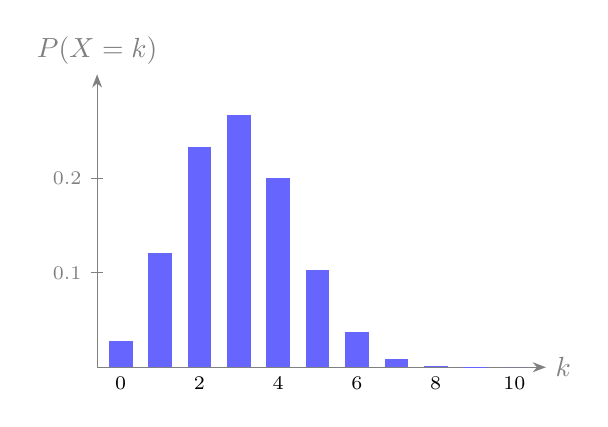
\begin{tikzpicture}[x=0.5cm, y=12cm, >=Stealth]
        \draw[->, gray] (-0.6,0) -- (10.8,0) node[right] {$k$};
        \draw[->, gray] (-0.6,0) -- (-0.6,0.31) node[above] {$P(X = k)$};
        \foreach \k/\v in {0/0.0282, 1/0.1211, 2/0.2335, 3/0.2668, 4/0.2001, 5/0.1029, 6/0.0368, 7/0.0090, 8/0.0014, 9/0.0001, 10/0.0}
            \fill[blue!60] (\k-0.3,0) rectangle (\k+0.3,\v);
        \foreach \k in {0,2,...,10}
            \node[below, font=\scriptsize] at (\k,0) {$\k$};
        \foreach \v in {0.1,0.2}
            \draw[gray] (-0.75,\v) -- (-0.45,\v) node[pos=0, left, font=\scriptsize] {$\v$};
    \end{tikzpicture}
    \qquad
    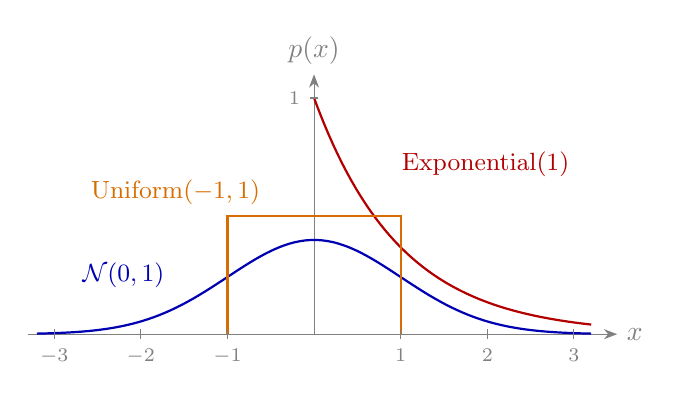
\begin{tikzpicture}[x=1.1cm, y=3cm, >=Stealth]
        \draw[->, gray] (-3.3,0) -- (3.5,0) node[right] {$x$};
        \draw[->, gray] (0,0) -- (0,1.1) node[above] {$p(x)$};
        \draw[blue!70!black, thick, domain=-3.2:3.2, samples=100] plot (\x, {exp(-(\x)^2/2)/sqrt(2*pi)});
        \draw[red!70!black, thick, domain=0:3.2, samples=60] plot (\x, {exp(-\x)});
        \draw[orange!85!black, thick] (-1,0) -- (-1,0.5) -- (1,0.5) -- (1,0);
        \foreach \x in {-3,-2,-1,1,2,3}
            \draw[gray] (\x,0.02) -- (\x,-0.02) node[below, font=\scriptsize] {$\x$};
        \draw[gray] (0.05,1) -- (-0.05,1) node[left, font=\scriptsize] {$1$};
        \node[blue!70!black, font=\small] at (-2.2,0.25) {$\mathcal{N}(0, 1)$};
        \node[red!70!black, font=\small, right] at (0.9,0.72) {Exponential$(1)$};
        \node[orange!85!black, font=\small] at (-1.6,0.6) {Uniform$(-1, 1)$};
    \end{tikzpicture}
    \caption{Left: the pmf of the Binomial$(10, 0.3)$ distribution. Right: the densities of the standard normal distribution, the Exponential$(1)$ distribution and the Uniform$(-1, 1)$ distribution.}
    \label{L4-fig:distributions}
\end{figure}

\subsection{Transformations of random variables}

If $X$ is a random variable and $g: \mathbb{R} \to \mathbb{R}$ is a function, then $Y = g(X)$ is again a random variable. For continuous random variables and invertible $g$, the density changes by the derivative of $g$, just as areas change by the Jacobian determinant in Lecture~3.

\begin{proposition}[Change of variables]\label{L4-prop:change-of-variables-1d}
    Let $X$ have the density $p_X$, and let $g$ be differentiable and strictly increasing (or strictly decreasing). Then $Y = g(X)$ has the density
    \[p_Y(y) = p_X(x)\,\frac{1}{|g'(x)|}, \qquad \text{where } x = g^{-1}(y).\]
\end{proposition}

\begin{proof}
    For increasing $g$, $F_Y(y) = P(g(X) \leq y) = P(X \leq g^{-1}(y)) = F_X(g^{-1}(y))$. Differentiating with the chain rule gives $p_Y(y) = p_X(g^{-1}(y))\,(g^{-1})'(y) = \frac{p_X(x)}{g'(x)}$. For decreasing $g$, $F_Y(y) = 1 - F_X(g^{-1}(y))$, which gives the same formula with $|g'(x)|$.
\end{proof}

\begin{example}\label{L4-ex:transformations}
    \begin{enumerate}
        \item (Standardization.) If $X \sim \mathcal{N}(\mu, \sigma^2)$, then $Z = \frac{X - \mu}{\sigma}$ has the density $\sigma\,p_X(\mu + \sigma z) = \varphi(z)$, so $Z \sim \mathcal{N}(0, 1)$. Conversely, $X = \mu + \sigma Z$. Hence $P(|X - \mu| \leq k\sigma) = P(|Z| \leq k)$, which is $0.683$, $0.954$ and $0.997$ for $k = 1, 2, 3$, and $0.95$ for $k = 1.96$.
        \item (Log-normal distribution.) If $X \sim \mathcal{N}(0, 1)$, then $Y = e^X$ has the density $\frac{\varphi(\log y)}{y}$ for $y > 0$.
    \end{enumerate}
\end{example}

\begin{theorem}[Inverse transform sampling]\label{L4-thm:inverse-transform}
    Let $F$ be nondecreasing and right-continuous with the limits $0$ at $-\infty$ and $1$ at $\infty$, let
    \[F^{-1}(u) = \min\{x \in \mathbb{R} : F(x) \geq u\} \qquad \text{for } 0 < u < 1\]
    be its quantile function, and let $U \sim$ Uniform$(0, 1)$. Then $X = F^{-1}(U)$ has the CDF $F$.
\end{theorem}

\begin{proof}
    For $0 < u < 1$, the set $\{x : F(x) \geq u\}$ is nonempty and bounded below, since $F$ tends to $1$ and to $0$. Since $F$ is nondecreasing, it is an interval that extends to $\infty$, and since $F$ is right-continuous, it contains its left endpoint. So the minimum exists, and $F^{-1}(u) \leq x$ if and only if $F(x) \geq u$. Hence $P(X \leq x) = P(U \leq F(x)) = F(x)$.
\end{proof}

If $F$ is continuous and strictly increasing, $F^{-1}$ is the inverse function of $F$. So a computer that can generate uniform random numbers can generate random numbers with any distribution on $\mathbb{R}$, and the random variable $F^{-1}(U)$ on the probability space $\big((0, 1), \mathcal{B}, \lambda\big)$, with $U(\omega) = \omega$, proves the last part of Theorem~\ref{L4-thm:cdf}. For example, the Exponential$(\lambda)$ distribution has $F(x) = 1 - e^{-\lambda x}$, so $X = -\frac{1}{\lambda}\log(1 - U)$ is exponentially distributed. For a Bernoulli$(p)$ variable, $F$ jumps from $0$ to $1 - p$ at $0$ and from $1 - p$ to $1$ at $1$, so $F^{-1}(u) = 0$ for $u \leq 1 - p$ and $F^{-1}(u) = 1$ for $u > 1 - p$: we return $1$ if $U > 1 - p$, which has the probability $p$. Normalizing flows (Lecture~3) generalize this idea to many dimensions: they transform simple random vectors by learned invertible maps.

\section{Expectation and Integration}\label{L4-sec:expectation}

The expectation of a random variable is its average value, weighted by probability. For a random variable with finitely many values $x_1, \ldots, x_k$, it is the sum $\sum_i x_iP(X = x_i)$. In general, it is an integral with respect to the probability measure $P$, the Lebesgue integral. The construction works for every measure, and for the Lebesgue measure on $\mathbb{R}^n$, it extends the integral of Lecture~3.

\subsection{The Lebesgue integral}\label{L4-sec:lebesgue}

Let $(\Omega, \mathcal{F}, \mu)$ be a measure space. A function $f: \Omega \to \mathbb{R}$ or $f: \Omega \to [0, \infty]$ is measurable if $\{f \leq x\} \in \mathcal{F}$ for all $x \in \mathbb{R}$; on a probability space, the measurable real-valued functions are the random variables.

\begin{definition}[Lebesgue integral]\label{L4-def:lebesgue}
    \begin{enumerate}
        \item A simple function is a finite sum $s = \sum_{i=1}^k a_i\mathbf{1}_{A_i}$ with $a_i \geq 0$ and $A_i \in \mathcal{F}$, and its integral is $\int s\, d\mu = \sum_{i=1}^k a_i\mu(A_i)$, with $0 \cdot \infty = 0$.
        \item For a measurable $f: \Omega \to [0, \infty]$,
        \[\int f\, d\mu = \sup\Big\{\int s\, d\mu : s \text{ simple, } 0 \leq s \leq f\Big\} \in [0, \infty].\]
        \item A measurable $f: \Omega \to \mathbb{R}$ is integrable if $\int |f|\, d\mu < \infty$, and then $\int f\, d\mu = \int f^+\, d\mu - \int f^-\, d\mu$, where $f^+ = \max(f, 0)$ and $f^- = \max(-f, 0)$, so that $f = f^+ - f^-$ and $|f| = f^+ + f^-$.
    \end{enumerate}
    For $A \in \mathcal{F}$, we write $\int_A f\, d\mu = \int f\mathbf{1}_A\, d\mu$. Other notations are $\int f(\omega)\, \mu(d\omega)$, and for the Lebesgue measure, $\int f(\mathbf{x})\, d\mathbf{x}$.
\end{definition}

(One checks that the integral of a simple function does not depend on how it is written as a sum.) The Riemann integral of Lecture~3 divides the domain into small boxes. The Lebesgue integral divides the range instead: the simple functions
\[s_n = \min\big(n, \, 2^{-n}\lfloor 2^nf\rfloor\big),\]
which round $f$ down to a multiple of $2^{-n}$ and cut it off at $n$, increase to $f$, and $\int s_n\, d\mu$ adds up the values $j2^{-n}$, weighted by the measures of the sets $\{j2^{-n} \leq f < (j + 1)2^{-n}\}$. One can show that the integral is linear and monotone ($f \leq g$ implies $\int f\, d\mu \leq \int g\, d\mu$), that $\int |f|\, d\mu = 0$ if and only if $f = 0$ almost everywhere, i.e., outside a set of measure $0$, and that functions which agree almost everywhere have the same integral. For bounded Riemann integrable functions on boxes, and for absolutely convergent improper Riemann integrals, the Lebesgue integral agrees with the Riemann integral. But it integrates many more functions. For example, the indicator function $\mathbf{1}_{\mathbb{Q}}$ of the rationals on $[0, 1]$ is not Riemann integrable, since every Riemann sum can be made $0$ or $1$ by choosing irrational or rational points, but its Lebesgue integral is $\lambda(\mathbb{Q} \cap [0, 1]) = 0$. For the counting measure on $\mathbb{N}$, the integral is a series: $\int f\, d\mu = \sum_k f(k)$.

\subsection{Expectation}

\begin{definition}[Expectation]\label{L4-def:expectation}
    The expectation (expected value, or mean) of a random variable $X$ on a probability space $(\Omega, \mathcal{F}, P)$ is
    \[\E[X] = \int X\, dP,\]
    defined if $X \geq 0$ (then possibly $\E[X] = \infty$) or if $X$ is integrable, i.e., $\E[|X|] < \infty$.
\end{definition}

The expectation is linear, $\E[aX + bY + c] = a\E[X] + b\E[Y] + c$, and monotone, since the integral is, and $\E[\mathbf{1}_A] = P(A)$ for every event $A$. It is the center of mass of the distribution: if we put the mass $P(X = x_i)$ at each value $x_i$, the balance point is $\E[X]$. To compute expectations, we do not need the sample space, only the distribution.

\begin{theorem}[Expectations from distributions]\label{L4-thm:lotus}
    Let $X$ be a random variable, and let $g: \mathbb{R} \to \mathbb{R}$ be measurable with $g \geq 0$ or $\E[|g(X)|] < \infty$. Then $\E[g(X)] = \int_{\mathbb{R}} g\, dP_X$. In particular,
    \[\E[g(X)] = \sum_i g(x_i)\,p(x_i) \qquad \text{or} \qquad \E[g(X)] = \int_{-\infty}^\infty g(x)\,p(x) \, dx\]
    for discrete $X$ with the pmf $p$ and continuous $X$ with the density $p$, respectively.
\end{theorem}

\begin{proof}
    For $g = \mathbf{1}_B$, both sides are $P(X \in B)$, by the definition of $P_X$. By linearity, the formula holds for simple functions $g$, and by the monotone convergence theorem below, applied to simple functions that increase to $g$, for all $g \geq 0$. For integrable $g(X)$, apply it to $g^+$ and $g^-$. The two formulas follow in the same way from Definition~\ref{L4-def:density} below, with the counting measure and the Lebesgue measure.
\end{proof}

\begin{example}[Tail sums]\label{L4-ex:tail-sum}
    Let $X$ take values in $\{0, 1, 2, \ldots\}$. Then $X = \sum_{k=0}^\infty \mathbf{1}_{\{X > k\}}$, since exactly the first $X$ terms are $1$. By the monotone convergence theorem below, the expectation of a series of nonnegative random variables is the series of their expectations, so
    \[\E[X] = \sum_{k=0}^\infty P(X > k).\]
    For a Geometric$(p)$ variable, $P(X > k) = (1 - p)^k$, the probability that the first $k$ trials fail, so $\E[X] = \sum_{k \geq 0}(1 - p)^k = \frac{1}{p}$. Example~\ref{L4-ex:tail-integral} gives the analogous formula for continuous random variables.
\end{example}

\subsection{Variance and moments}

\begin{definition}[Variance]\label{L4-def:variance}
    The variance of $X$ with mean $\mu = \E[X]$ is $\Var(X) = \E[(X - \mu)^2]$, and its standard deviation is $\sigma = \sqrt{\Var(X)}$.
\end{definition}

The variance measures how far $X$ typically is from its mean. Expanding the square and using linearity,
\[\Var(X) = \E[X^2 - 2\mu X + \mu^2] = \E[X^2] - 2\mu^2 + \mu^2 = \E[X^2] - \E[X]^2,\]
and $\Var(aX + b) = \E[(aX - a\mu)^2] = a^2\Var(X)$: shifting does not change the spread, and scaling by $a$ scales the standard deviation by $|a|$.

\begin{proposition}\label{L4-prop:moments}
    The distributions of Section~\ref{L4-sec:random-variables} have the following means and variances:
    \begin{center}
        \renewcommand{\arraystretch}{1.3}
        \begin{tabular}{lll}
            \hline
            distribution & $\E[X]$ & $\Var(X)$ \\
            \hline
            Bernoulli$(p)$ & $p$ & $p(1 - p)$ \\
            Binomial$(n, p)$ & $np$ & $np(1 - p)$ \\
            Geometric$(p)$ & $\frac{1}{p}$ & $\frac{1 - p}{p^2}$ \\
            Poisson$(\lambda)$ & $\lambda$ & $\lambda$ \\
            Uniform$(a, b)$ & $\frac{a + b}{2}$ & $\frac{(b - a)^2}{12}$ \\
            Exponential$(\lambda)$ & $\frac{1}{\lambda}$ & $\frac{1}{\lambda^2}$ \\
            $\mathcal{N}(\mu, \sigma^2)$ & $\mu$ & $\sigma^2$ \\
            \hline
        \end{tabular}
    \end{center}
\end{proposition}

\begin{proof}[Proof of some cases]
    Bernoulli: $\E[X] = 0 \cdot (1 - p) + 1 \cdot p = p$, and $X^2 = X$, so $\Var(X) = p - p^2$. Uniform: $\E[X] = \frac{1}{b - a}\int_a^b x\, dx = \frac{b^2 - a^2}{2(b - a)} = \frac{a + b}{2}$, and similarly $\E[X^2] = \frac{a^2 + ab + b^2}{3}$, so $\Var(X) = \frac{(b - a)^2}{12}$. Exponential: integrating by parts, $\E[X] = \int_0^\infty x\lambda e^{-\lambda x}\, dx = \big[-xe^{-\lambda x}\big]_0^\infty + \int_0^\infty e^{-\lambda x}\, dx = \frac{1}{\lambda}$. Poisson: $\E[X] = \sum_{k \geq 1} k e^{-\lambda}\frac{\lambda^k}{k!} = \lambda\sum_{k \geq 1} e^{-\lambda}\frac{\lambda^{k-1}}{(k-1)!} = \lambda$. Normal: by Example~\ref{L4-ex:transformations}, $X = \mu + \sigma Z$ with $Z \sim \mathcal{N}(0, 1)$, so it suffices to show $\E[Z] = 0$ and $\Var(Z) = 1$. The first holds since $z\varphi(z)$ is an odd function, and for the second, integration by parts with $\varphi'(z) = -z\varphi(z)$ gives
    \[\E[Z^2] = \int_{-\infty}^\infty z \cdot z\varphi(z) \, dz = \big[-z\varphi(z)\big]_{-\infty}^\infty + \int_{-\infty}^\infty \varphi(z) \, dz = 1.\]
    The binomial case follows from the Bernoulli case and Proposition~\ref{L4-prop:variance-sum} below.
\end{proof}

\begin{example}\label{L4-ex:die-moments}
    For a fair die, $\E[X] = \frac{1 + 2 + \cdots + 6}{6} = 3.5$, which is not a possible value, and $\E[X^2] = \frac{91}{6}$, so $\Var(X) = \frac{91}{6} - \frac{49}{4} = \frac{35}{12} \approx 2.92$.
\end{example}

\subsection{Convergence theorems}

When can we exchange a limit and an expectation? This question comes up constantly: for limits of random variables, for infinite series, and for derivatives of expectations with respect to parameters. The answer is the main advantage of the Lebesgue integral.

\begin{theorem}[Monotone convergence]\label{L4-thm:monotone}
    Let $0 \leq f_1 \leq f_2 \leq \cdots$ be measurable functions with $f_n \to f$ pointwise. Then $\int f_n\, d\mu \to \int f\, d\mu$.
\end{theorem}

\begin{proof}
    By monotonicity, the integrals $\int f_n\, d\mu$ increase to a limit $L \leq \int f\, d\mu$. Conversely, let $s = \sum_i a_i\mathbf{1}_{A_i}$ be simple with $0 \leq s \leq f$, and let $0 < c < 1$. The sets $E_n = \{f_n \geq cs\}$ increase to $\Omega$: where $s > 0$, we have $f_n \to f \geq s > cs$, and where $s = 0$, trivially $f_n \geq cs$. Hence
    \[\int f_n\, d\mu \geq \int cs\mathbf{1}_{E_n}\, d\mu = c\sum_i a_i\mu(A_i \cap E_n) \to c\int s\, d\mu,\]
    by the continuity of measures (Proposition~\ref{L4-prop:probability-rules}(5), whose proof works for every measure). So $L \geq c\int s\, d\mu$ for all $c < 1$ and all such $s$, i.e., $L \geq \int f\, d\mu$.
\end{proof}

\begin{theorem}[Fatou's lemma and dominated convergence]\label{L4-thm:dominated}
    \begin{enumerate}
        \item (Fatou) For measurable $f_n \geq 0$, $\int \liminf_n f_n\, d\mu \leq \liminf_n \int f_n\, d\mu$.
        \item (Dominated convergence) Let $f_n \to f$ pointwise (or almost everywhere), and let $|f_n| \leq g$ for all $n$, with an integrable function $g$. Then $f$ is integrable, and $\int f_n\, d\mu \to \int f\, d\mu$.
    \end{enumerate}
\end{theorem}

\begin{proof}
    (1) The functions $g_k = \inf_{n \geq k} f_n$ increase to $\liminf_n f_n$, and $\int g_k\, d\mu \leq \int f_n\, d\mu$ for all $n \geq k$. By monotone convergence, $\int \liminf_n f_n\, d\mu = \lim_k \int g_k\, d\mu \leq \liminf_n \int f_n\, d\mu$. (2) Since $|f| \leq g$, $f$ is integrable. Fatou's lemma, applied to the nonnegative functions $g + f_n$ and $g - f_n$, gives
    \[\int g\, d\mu + \int f\, d\mu \leq \int g\, d\mu + \liminf_n \int f_n\, d\mu \qquad \text{and} \qquad \int g\, d\mu - \int f\, d\mu \leq \int g\, d\mu - \limsup_n \int f_n\, d\mu.\]
    Hence $\limsup_n \int f_n\, d\mu \leq \int f\, d\mu \leq \liminf_n \int f_n\, d\mu$.
\end{proof}

\begin{example}\label{L4-ex:escaping-mass}
    \begin{enumerate}
        \item (Mass can escape.) On $[0, 1]$ with the Lebesgue measure, let $f_n = n\mathbf{1}_{(0, 1/n)}$. Then $f_n(x) \to 0$ for every $x$, but $\int f_n\, d\lambda = 1$ for all $n$: the limit of the integrals is not the integral of the limit. In the language of probability, $X_n = n\mathbf{1}_{\{U < 1/n\}}$ for a uniform $U$ is a lottery ticket that wins $n$ euros with probability $\frac{1}{n}$; it is $0$ for all large $n$, but $\E[X_n] = 1$. Dominated convergence does not apply, since $\sup_n f_n(x) \geq \frac{1}{2x}$ for $0 < x \leq \frac{1}{2}$, which is not integrable.
        \item (Differentiating under the integral sign.) Let $f(x, \theta)$ be integrable in $x$ and differentiable in $\theta$, with $|\frac{\partial f}{\partial\theta}(x, \theta)| \leq g(x)$ for all $\theta$ in an open interval, where $\int g\, d\mu < \infty$. Then
        \[\frac{d}{d\theta}\int f(x, \theta)\, d\mu(x) = \int \frac{\partial f}{\partial\theta}(x, \theta)\, d\mu(x).\]
        Indeed, for $h_n \to 0$, the difference quotients $\frac{f(x, \theta + h_n) - f(x, \theta)}{h_n}$ converge to $\frac{\partial f}{\partial\theta}(x, \theta)$, and by the mean value theorem, they are bounded by $g(x)$; now apply dominated convergence. This proves the Leibniz rule (Proposition~\ref{L3-prop:leibniz}) for unbounded regions, under the condition stated there, and for general measures. It also shows that the gradient of an expected loss is the expected gradient, $\nabla_{\boldsymbol{\theta}}\E[\ell(\boldsymbol{\theta}; \mathbf{X})] = \E[\nabla_{\boldsymbol{\theta}}\ell(\boldsymbol{\theta}; \mathbf{X})]$, if the partial derivatives are dominated in this way. This is why the gradient on a random training example is an unbiased estimate of the gradient of the expected loss.
    \end{enumerate}
\end{example}

\subsection{Densities and the Radon--Nikodym theorem}\label{L4-sec:densities}

Discrete and continuous distributions look different, but they are two cases of one notion.

\begin{definition}[Density with respect to a measure]\label{L4-def:density}
    Let $\mu$ be a measure on $(\mathbb{R}^n, \mathcal{B}(\mathbb{R}^n))$. A random vector $\mathbf{X}$, or its distribution, has the density $p \geq 0$ with respect to $\mu$ if
    \[P(\mathbf{X} \in B) = \int_B p\, d\mu \qquad \text{for all Borel sets } B.\]
    Then $\E[g(\mathbf{X})] = \int g\,p\, d\mu$ for every measurable $g \geq 0$, by the argument of Theorem~\ref{L4-thm:lotus}.
\end{definition}

For the Lebesgue measure, $p$ is the density of Section~\ref{L4-sec:random-variables}. For the counting measure on a countable set $\{x_1, x_2, \ldots\}$ of values, $\int_B p\, d\mu = \sum_{x_i \in B} p(x_i)$, so $p$ is the pmf. So sums with pmfs and integrals with pdfs are integrals with respect to different reference measures, and everything that we prove for integrals holds for both. A necessary condition for a density is that $\mu(B) = 0$ implies $P(\mathbf{X} \in B) = 0$, since an integral over a null set is $0$. The distribution is then called absolutely continuous with respect to $\mu$, and this condition is also sufficient.

\begin{theorem}[Radon--Nikodym]\label{L4-thm:radon-nikodym}
    Let $\mu$ and $\nu$ be $\sigma$-finite measures on $(\Omega, \mathcal{F})$ such that $\mu(A) = 0$ implies $\nu(A) = 0$ (written $\nu \ll \mu$). Then there is a measurable $p \geq 0$ with $\nu(A) = \int_A p\, d\mu$ for all $A \in \mathcal{F}$, and $p$ is unique up to changes on a set of $\mu$-measure $0$. It is called the Radon--Nikodym derivative $\frac{d\nu}{d\mu}$.
\end{theorem}

We do not prove this theorem here; Appendix~\ref{A-chapter} proves it with the Riesz representation theorem for Hilbert spaces. Not every distribution has a density with respect to the Lebesgue measure or a counting measure.

\begin{example}[The ReLU of a Gaussian]\label{L4-ex:relu-gaussian}
    Let $Z \sim \mathcal{N}(0, 1)$, and let $Y = \max(0, Z)$ be the activation of a ReLU unit with a Gaussian input. Then $P(Y = 0) = P(Z \leq 0) = \frac{1}{2}$, and $P(a \leq Y \leq b) = \int_a^b \varphi(y)\, dy$ for $0 < a < b$. So $Y$ is neither discrete nor continuous: it has an atom of mass $\frac{1}{2}$ at $0$, which the Lebesgue measure does not see. But $Y$ has a density with respect to $\mu = \delta_0 + \lambda$, namely $p(0) = \frac{1}{2}$ and $p(y) = \varphi(y)\mathbf{1}_{\{y > 0\}}$ for $y \neq 0$. Hence
    \[\E[Y] = 0 \cdot \tfrac{1}{2} + \int_0^\infty y\varphi(y)\, dy = \frac{1}{\sqrt{2\pi}} \approx 0.399, \qquad \E[Y^2] = \int_0^\infty y^2\varphi(y)\, dy = \frac{1}{2},\]
    so $\Var(Y) = \frac{1}{2} - \frac{1}{2\pi} \approx 0.341$. Mixed distributions of this kind also describe zero-inflated data, such as daily rainfall, or the amount that a visitor of a web shop spends.
\end{example}

\begin{remark}[Singular distributions and likelihood ratios]\label{L4-rem:singular}
    \begin{enumerate}
        \item Some distributions have neither atoms nor a density with respect to the Lebesgue measure. An example is the Cantor distribution, the distribution of $X = \sum_{k=1}^\infty 2D_k3^{-k}$ with independent fair coin flips $D_k \in \{0, 1\}$, a random number whose ternary digits are all $0$ or $2$. Its CDF, the Cantor function, is continuous, so $X$ has no atoms. But $X$ lies in the Cantor set, which has Lebesgue measure $0$, so it has no density. One can show that every distribution on $\mathbb{R}$ is a mixture of a discrete, an absolutely continuous, and such a singular part (the Lebesgue decomposition).
        \item If $P \ll Q$, the Radon--Nikodym derivative $\frac{dP}{dQ}$ is the likelihood ratio, which is $\frac{p}{q}$ if $P$ and $Q$ have the densities $p$ and $q$. The weights of importance sampling (Section~\ref{L4-sec:monte-carlo}) are likelihood ratios, $\E_P[f] = \E_Q[f\frac{dP}{dQ}]$, and the KL divergence of Section~\ref{L4-sec:information} is $\KL(P \,\|\, Q) = \E_P[\log\frac{dP}{dQ}]$ for $P \ll Q$, and $\infty$ otherwise. So these notions make sense for arbitrary distributions.
    \end{enumerate}
\end{remark}

\subsection{Inequalities}

The variance controls how likely large deviations from the mean are.

\begin{proposition}[Markov and Chebyshev]\label{L4-prop:markov}
    \begin{enumerate}
        \item (Markov's inequality.) If $X \geq 0$ and $a > 0$, then $P(X \geq a) \leq \frac{\E[X]}{a}$.
        \item (Chebyshev's inequality.) If $X$ has mean $\mu$ and variance $\sigma^2$, then $P(|X - \mu| \geq k) \leq \frac{\sigma^2}{k^2}$ for every $k > 0$.
    \end{enumerate}
\end{proposition}

\begin{proof}
    (1) Since $X \geq 0$, we have $X \geq a\mathbf{1}_{\{X \geq a\}}$. Taking expectations, $\E[X] \geq a P(X \geq a)$. (2) Apply (1) to $(X - \mu)^2$ and $a = k^2$: $P(|X - \mu| \geq k) = P((X - \mu)^2 \geq k^2) \leq \frac{\sigma^2}{k^2}$.
\end{proof}

For example, every random variable is at least $2$ standard deviations from its mean with probability at most $\frac{1}{4}$. This bound holds for all distributions, so it is weak for specific ones: for a normal distribution, the probability is only $0.046$.

\begin{theorem}[Jensen's inequality]\label{L4-thm:jensen}
    If $f$ is convex, then $f(\E[X]) \leq \E[f(X)]$. If $f$ is concave, then $f(\E[X]) \geq \E[f(X)]$.
\end{theorem}

\begin{proof}
    We prove this for differentiable $f$. Let $\mu = \E[X]$. By the first-order characterization of convexity in Lecture~3, $f(x) \geq f(\mu) + f'(\mu)(x - \mu)$ for all $x$. So $f(X) \geq f(\mu) + f'(\mu)(X - \mu)$, and taking expectations gives $\E[f(X)] \geq f(\mu) + f'(\mu) \cdot 0$. For concave $f$, apply this to $-f$.
\end{proof}

For example, $f(x) = x^2$ gives $\E[X]^2 \leq \E[X^2]$, i.e., $\Var(X) \geq 0$, and the concave function $\log$ gives $\E[\log X] \leq \log\E[X]$ for $X > 0$. We will use the latter to show that the Kullback--Leibler divergence is nonnegative (Section~\ref{L4-sec:information}).

\begin{example}[The Chernoff bound]\label{L4-ex:chernoff}
    Markov's inequality becomes much stronger when it is applied to an exponential: for every $t > 0$, $P(X \geq a) = P(e^{tX} \geq e^{ta}) \leq e^{-ta}\E[e^{tX}]$, and we may choose the best $t$. For $S \sim$ Binomial$(n, \frac{1}{2})$, the sum of $n$ independent fair coin flips, $\E[e^{tS}] = \big(\frac{1 + e^t}{2}\big)^n$ (by Proposition~\ref{L4-prop:independent-product} below). For $n = 100$ and $a = 60$, the best choice is $e^t = \frac{3}{2}$, which gives $P(S \geq 60) \leq \big(\frac{5}{4}\big)^{100}\big(\frac{2}{3}\big)^{60} \approx 0.134$, while Chebyshev's inequality only gives $P(S \geq 60) \leq P(|S - 50| \geq 10) \leq \frac{25}{100} = 0.25$; the exact value is $0.028$. As $n$ grows, Chernoff bounds decrease exponentially, while Chebyshev's bound only decreases like $\frac{1}{n}$. Hoeffding's inequality (Theorem~\ref{L4-thm:hoeffding}) is proved in this way.
\end{example}

\paragraph{$L^p$ spaces.} For $p \geq 1$, the random variables with $\E[|X|^p] < \infty$ form a vector space $L^p$, and $\norm{X}_p = \E[|X|^p]^{1/p}$ is a norm on it, if we do not distinguish random variables that are equal almost surely (the triangle inequality is Minkowski's inequality, which we do not prove). By Jensen's inequality for the convex function $y \mapsto y^{q/p}$ on $[0, \infty)$, $\norm{X}_p \leq \norm{X}_q$ for $p \leq q$, so $L^q \subseteq L^p$. The space $L^2$, with the inner product $\E[XY]$, is complete, which makes it a Hilbert space (see Appendix~\ref{A-chapter}); we use this for the conditional expectation in Section~\ref{L4-sec:conditional-expectation}.

\section{Joint Distributions and Independence}\label{L4-sec:joint}

To describe how several random variables depend on each other, we need their joint distribution. A random vector $\mathbf{X} = (X_1, \ldots, X_n)$ is a measurable map from $\Omega$ to $\mathbb{R}^n$, i.e., $\{\mathbf{X} \in B\} \in \mathcal{F}$ for all Borel sets $B \subseteq \mathbb{R}^n$; one can show that this holds if and only if every $X_i$ is a random variable. Its joint distribution is the probability measure $P_{\mathbf{X}}(B) = P(\mathbf{X} \in B)$ on $\mathbb{R}^n$, and the distributions of the $X_i$ are its marginals. For two random variables, we describe them by pmfs and densities.

\begin{definition}[Joint, marginal and conditional distributions]\label{L4-def:joint}
    The joint pmf of two discrete random variables $X$ and $Y$ is $p(x, y) = P(X = x, Y = y)$. Two continuous random variables have a joint density $p(x, y) \geq 0$ if $P((X, Y) \in A) = \iint_A p(x, y) \, dx \, dy$ for all Borel sets $A \subseteq \mathbb{R}^2$. The marginal distributions of $X$ and $Y$ are
    \[p_X(x) = \sum_y p(x, y) \qquad \text{or} \qquad p_X(x) = \int_{-\infty}^\infty p(x, y) \, dy,\]
    and similarly for $p_Y$. The conditional distribution of $Y$ given $X = x$ (for $p_X(x) > 0$) is
    \[p(y \mid x) = \frac{p(x, y)}{p_X(x)}.\]
\end{definition}

The formulas $p_X(x) = \sum_y p(x, y)$ (the sum rule) and $p(x, y) = p(y \mid x)\,p_X(x)$ (the product rule) are the two basic rules of probabilistic machine learning, and Bayes' theorem $p(x \mid y) = \frac{p(y \mid x)p_X(x)}{p_Y(y)}$ follows from them. The same definitions apply to more than two random variables.

\paragraph{Product measures and independence.} On a product of two measure spaces, there is a natural measure.

\begin{theorem}[Product measures and Fubini--Tonelli]\label{L4-thm:fubini-tonelli}
    Let $\mu$ and $\nu$ be $\sigma$-finite measures on $(\Omega_1, \mathcal{F}_1)$ and $(\Omega_2, \mathcal{F}_2)$, and let $\mathcal{F}_1 \otimes \mathcal{F}_2$ be the $\sigma$-algebra on $\Omega_1 \times \Omega_2$ generated by the products $A \times B$ with $A \in \mathcal{F}_1$ and $B \in \mathcal{F}_2$. There is exactly one measure $\mu \otimes \nu$ on it with $(\mu \otimes \nu)(A \times B) = \mu(A)\nu(B)$, the product measure. For every measurable $f \geq 0$ (Tonelli), and for every $f$ that is integrable with respect to $\mu \otimes \nu$ (Fubini),
    \[\int f\, d(\mu \otimes \nu) = \int\bigg(\int f(x, y)\, d\nu(y)\bigg) d\mu(x) = \int\bigg(\int f(x, y)\, d\mu(x)\bigg) d\nu(y).\]
\end{theorem}

We do not prove this theorem. The Lebesgue measure on $\mathbb{R}^2$ is $\lambda \otimes \lambda$, and the theorem contains Fubini's theorem of Lecture~3, including its condition: for nonnegative functions, the order of integration never matters, and for functions of both signs, it does not matter if $\int |f| < \infty$ (compare with Example~\ref{L3-ex:fubini}, in which the two orders give $\frac{\pi}{4}$ and $-\frac{\pi}{4}$).

\begin{definition}[Independent random variables]\label{L4-def:independent-rv}
    Random variables $X_1, \ldots, X_n$ are independent if
    \[P(X_1 \in B_1, \ldots, X_n \in B_n) = P(X_1 \in B_1)\cdots P(X_n \in B_n) \qquad \text{for all Borel sets } B_1, \ldots, B_n,\]
    i.e., if their joint distribution is the product $P_{X_1} \otimes \cdots \otimes P_{X_n}$ of their distributions. Infinitely many random variables are independent if any finitely many of them are. They are independent and identically distributed (i.i.d.) if moreover they all have the same distribution.
\end{definition}

For discrete random variables, independence means $p(x, y) = p_X(x)\,p_Y(y)$ for all values $x$ and $y$, and for random variables with a joint density, it means that the joint density factorizes as $p(x, y) = p_X(x)\,p_Y(y)$ (outside a null set); equivalently, $p(y \mid x) = p_Y(y)$ whenever $p_X(x) > 0$. In the language of $\sigma$-algebras, the information contained in $X$ is the $\sigma$-algebra $\sigma(X) = \{\{X \in B\} : B \text{ Borel}\}$ generated by $X$, and $X$ and $Y$ are independent if and only if $\sigma(X)$ and $\sigma(Y)$ are independent (Definition~\ref{L4-def:independence}). Since $\sigma(g(X)) \subseteq \sigma(X)$ for measurable $g$, functions $g(X)$ and $h(Y)$ of independent random variables are again independent.

The standard assumption in machine learning is that the training examples are i.i.d.\ samples from an unknown distribution: each example is drawn from the same distribution, independently of the others.

\begin{example}\label{L4-ex:joint-table}
    Let $X, Y \in \{0, 1\}$ have the joint pmf
    \begin{center}
        \renewcommand{\arraystretch}{1.2}
        \begin{tabular}{c|cc|c}
            & $Y = 0$ & $Y = 1$ & $p_X$ \\
            \hline
            $X = 0$ & $0.3$ & $0.2$ & $0.5$ \\
            $X = 1$ & $0.1$ & $0.4$ & $0.5$ \\
            \hline
            $p_Y$ & $0.4$ & $0.6$ &
        \end{tabular}
    \end{center}
    The marginals are the row and column sums. The conditional probabilities are $P(Y = 1 \mid X = 1) = \frac{0.4}{0.5} = 0.8$ and $P(Y = 1 \mid X = 0) = \frac{0.2}{0.5} = 0.4$. Since $p(1, 1) = 0.4 \neq 0.5 \cdot 0.6 = p_X(1)p_Y(1)$, $X$ and $Y$ are not independent: learning $X$ changes the probabilities of $Y$.
\end{example}

For a function $g(X, Y)$, Theorem~\ref{L4-thm:lotus} for random vectors gives $\E[g(X, Y)] = \int g\, dP_{(X, Y)}$, i.e., $\sum_{x, y} g(x, y)\,p(x, y)$ or the corresponding integral of the joint density.

\begin{proposition}\label{L4-prop:independent-product}
    If $X$ and $Y$ are independent, and $g(X)$ and $h(Y)$ are integrable (or nonnegative), then $\E[g(X)h(Y)] = \E[g(X)]\,\E[h(Y)]$. In particular, $\E[XY] = \E[X]\,\E[Y]$ for integrable $X$ and $Y$.
\end{proposition}

\begin{proof}
    The joint distribution is $P_X \otimes P_Y$, so by Theorem~\ref{L4-thm:lotus} and Tonelli's theorem (for nonnegative functions) or Fubini's theorem,
    \[\E[g(X)h(Y)] = \int\!\!\int g(x)h(y)\, dP_X(x)\, dP_Y(y) = \int g\, dP_X\int h\, dP_Y = \E[g(X)]\,\E[h(Y)]. \qedhere\]
\end{proof}

\begin{example}[Sums of independent random variables]\label{L4-ex:convolution}
    If $X$ and $Y$ are independent with the densities $p_X$ and $p_Y$, then $X + Y$ has the density
    \[p_{X+Y}(z) = \int_{-\infty}^\infty p_X(x)\,p_Y(z - x)\, dx,\]
    the convolution of $p_X$ and $p_Y$. Indeed, by Tonelli's theorem and the substitution $y = z - x$,
    \[P(X + Y \leq t) = \int\!\!\int \mathbf{1}_{\{x + y \leq t\}}\,p_X(x)\,p_Y(y)\, dy\, dx = \int_{-\infty}^t \int_{-\infty}^\infty p_X(x)\,p_Y(z - x)\, dx\, dz.\]
    For two independent Uniform$(0, 1)$ variables, the integrand is $1$ for $\max(0, z - 1) \leq x \leq \min(1, z)$ and $0$ otherwise, so $p_{X+Y}(z) = z$ for $0 \leq z \leq 1$ and $p_{X+Y}(z) = 2 - z$ for $1 \leq z \leq 2$: a triangular density, and $P(X + Y \leq \frac{1}{2}) = \frac{1}{8}$. For independent $X \sim$ Poisson$(\lambda)$ and $Y \sim$ Poisson$(\mu)$, the same computation with sums and the binomial theorem gives
    \[P(X + Y = n) = \sum_{k=0}^n e^{-\lambda}\frac{\lambda^k}{k!}\,e^{-\mu}\frac{\mu^{n-k}}{(n - k)!} = e^{-(\lambda + \mu)}\frac{(\lambda + \mu)^n}{n!},\]
    so $X + Y \sim$ Poisson$(\lambda + \mu)$. For example, if a website gets independent Poisson numbers of clicks from search engines and from ads, with the means $3$ and $2$ per minute, then the total number of clicks per minute is Poisson$(5)$.
\end{example}

\begin{example}[Tail integrals]\label{L4-ex:tail-integral}
    For a random variable $X \geq 0$, we have $X = \int_0^\infty \mathbf{1}_{\{t < X\}}\, dt$, and Tonelli's theorem for $P \otimes \lambda$ gives
    \[\E[X] = \int_0^\infty P(X > t)\, dt,\]
    the continuous version of Example~\ref{L4-ex:tail-sum}. For example, for $X \sim$ Exponential$(\lambda)$, $\E[X] = \int_0^\infty e^{-\lambda t}\, dt = \frac{1}{\lambda}$, without integration by parts. Similarly, $\E[X^p] = \int_0^\infty pt^{p-1}P(X > t)\, dt$ for $p > 0$, which computes moments from tail bounds.
\end{example}

\subsection{Covariance and correlation}

\begin{definition}[Covariance and correlation]\label{L4-def:covariance}
    The covariance of $X$ and $Y$, with means $\mu_X$ and $\mu_Y$, is
    \[\Cov(X, Y) = \E[(X - \mu_X)(Y - \mu_Y)] = \E[XY] - \E[X]\,\E[Y],\]
    and if both have positive variances, their correlation is $\Corr(X, Y) = \frac{\Cov(X, Y)}{\sigma_X\sigma_Y}$. If $\Cov(X, Y) = 0$, they are uncorrelated.
\end{definition}

The covariance is positive if $X$ and $Y$ tend to be larger than their means at the same time, and negative if one tends to be large when the other is small. Note that $\Cov(X, X) = \Var(X)$, and the covariance is bilinear and symmetric. By Proposition~\ref{L4-prop:independent-product}, independent random variables are uncorrelated. The converse is false: if $X$ is uniform on $\{-1, 0, 1\}$ and $Y = X^2$, then $\Cov(X, Y) = \E[X^3] - \E[X]\E[X^2] = 0$, but $Y$ is a function of $X$. Correlation only measures linear dependence.

\begin{proposition}\label{L4-prop:variance-sum}
    $\Var(X + Y) = \Var(X) + \Var(Y) + 2\Cov(X, Y)$. In particular, if $X_1, \ldots, X_n$ are pairwise uncorrelated (for example, independent), then $\Var(X_1 + \cdots + X_n) = \Var(X_1) + \cdots + \Var(X_n)$.
\end{proposition}

\begin{proof}
    With $\tilde X = X - \mu_X$ and $\tilde Y = Y - \mu_Y$: $\Var(X + Y) = \E[(\tilde X + \tilde Y)^2] = \E[\tilde X^2] + \E[\tilde Y^2] + 2\E[\tilde X\tilde Y]$. The second statement follows by induction.
\end{proof}

For example, a Binomial$(n, p)$ random variable is the sum of $n$ independent Bernoulli$(p)$ random variables, so its mean is $np$ and its variance is $np(1 - p)$, as claimed in Proposition~\ref{L4-prop:moments}.

The covariance behaves like an inner product. For random variables $U$ and $V$ with finite variances, $\ip{U}{V} = \E[UV]$ is bilinear, symmetric, and $\ip{U}{U} = \E[U^2] \geq 0$, with equality only if $U = 0$ with probability $1$. So, if we do not distinguish random variables that are equal with probability $1$, it is an inner product as in Lecture~2: the inner product of the space $L^2$ of Section~\ref{L4-sec:expectation}. For centered random variables, the inner product is the covariance, the norm is the standard deviation, and the correlation is the cosine of the angle between them.

\begin{theorem}\label{L4-thm:correlation}
    $|\Cov(X, Y)| \leq \sigma_X\sigma_Y$, i.e., $-1 \leq \Corr(X, Y) \leq 1$. Moreover, $|\Corr(X, Y)| = 1$ if and only if $Y = aX + b$ with probability $1$, for some $a \neq 0$ and $b$; the sign of the correlation is the sign of $a$.
\end{theorem}

\begin{proof}
    This is the Cauchy--Schwarz inequality for the centered random variables $\tilde X$ and $\tilde Y$. Directly: for every $t \in \mathbb{R}$,
    \[0 \leq \E[(\tilde Y - t\tilde X)^2] = \sigma_Y^2 - 2t\Cov(X, Y) + t^2\sigma_X^2.\]
    A quadratic polynomial in $t$ that is never negative has a discriminant $\leq 0$, so $4\Cov(X, Y)^2 - 4\sigma_X^2\sigma_Y^2 \leq 0$. Equality holds if and only if the polynomial has a zero $t = a$, i.e., $\E[(\tilde Y - a\tilde X)^2] = 0$, i.e., $\tilde Y = a\tilde X$ with probability $1$; then $Y = aX + (\mu_Y - a\mu_X)$, and $\Cov(X, Y) = a\sigma_X^2$.
\end{proof}

\begin{example}\label{L4-ex:joint-cov}
    In Example~\ref{L4-ex:joint-table}, $\E[XY] = P(X = 1, Y = 1) = 0.4$, so $\Cov(X, Y) = 0.4 - 0.5 \cdot 0.6 = 0.1$. With $\Var(X) = 0.25$ and $\Var(Y) = 0.24$, the correlation is $\frac{0.1}{\sqrt{0.06}} \approx 0.41$.
\end{example}

\subsection{Conditional expectation}\label{L4-sec:conditional-expectation}

\begin{definition}[Conditional expectation]\label{L4-def:conditional-expectation}
    The conditional expectation of $Y$ given $X = x$ is the mean of the conditional distribution,
    \[m(x) = \E[Y \mid X = x] = \sum_y y\,p(y \mid x) \qquad \text{or} \qquad \int_{-\infty}^\infty y\,p(y \mid x) \, dy.\]
    The random variable $\E[Y \mid X] = m(X)$ is the conditional expectation of $Y$ given $X$.
\end{definition}

\begin{theorem}\label{L4-thm:conditional-expectation}
    \begin{enumerate}
        \item (Tower property.) $\E\big[\E[Y \mid X]\big] = \E[Y]$.
        \item (Best prediction.) For every function $g$, $\E[(Y - g(X))^2] \geq \E[(Y - m(X))^2]$, with $m(x) = \E[Y \mid X = x]$. More precisely,
        \[\E[(Y - g(X))^2] = \E[(Y - m(X))^2] + \E[(m(X) - g(X))^2].\]
    \end{enumerate}
\end{theorem}

\begin{proof}
    We give the proof for discrete random variables. (1) $\E[m(X)] = \sum_x p_X(x)\sum_y y\,p(y \mid x) = \sum_{x, y} y\,p(x, y) = \E[Y]$. (2) For every function $h$, the error $Y - m(X)$ is orthogonal to $h(X)$:
    \[\E[(Y - m(X))h(X)] = \sum_x p_X(x)h(x)\sum_y (y - m(x))p(y \mid x) = \sum_x p_X(x)h(x)\big(m(x) - m(x)\big) = 0.\]
    Now write $Y - g(X) = (Y - m(X)) + (m(X) - g(X))$, expand the square, and use this with $h = m - g$; the mixed term vanishes, as in the theorem of Pythagoras.
\end{proof}

So $\E[Y \mid X]$ is the best prediction of $Y$ from $X$ in the sense of the mean squared error: it is the orthogonal projection of $Y$ onto the space of functions of $X$, with respect to the inner product $\E[UV]$ (compare with orthogonal projections in Lecture~2). A regression model trained with the squared loss on enough data therefore estimates the conditional mean $\E[Y \mid X = \mathbf{x}]$. In Example~\ref{L4-ex:joint-table}, $\E[Y \mid X = 0] = 0.4$ and $\E[Y \mid X = 1] = 0.8$, and indeed $0.5 \cdot 0.4 + 0.5 \cdot 0.8 = 0.6 = \E[Y]$.

\paragraph{Conditioning on information.} The conditional expectation $\E[Y \mid X]$ only depends on the information contained in $X$: it is a function of $X$, and by the proof of Theorem~\ref{L4-thm:conditional-expectation}, $\E\big[(Y - \E[Y \mid X])\mathbf{1}_G\big] = 0$ for every event $G = \{X \in B\}$ in $\sigma(X)$. These two properties define the conditional expectation in general: also when $P(X = x) = 0$ for all $x$ and there is no joint density, and for conditioning on infinitely many random variables.

\begin{definition}[Conditional expectation given a $\sigma$-algebra]\label{L4-def:conditional-expectation-general}
    Let $Y$ be integrable, and let $\mathcal{G} \subseteq \mathcal{F}$ be a $\sigma$-algebra. A conditional expectation of $Y$ given $\mathcal{G}$ is a $\mathcal{G}$-measurable integrable random variable $\E[Y \mid \mathcal{G}]$ with
    \[\E\big[\E[Y \mid \mathcal{G}]\,\mathbf{1}_G\big] = \E[Y\mathbf{1}_G] \qquad \text{for all } G \in \mathcal{G}.\]
    For a random variable or random vector $X$, $\E[Y \mid X] = \E[Y \mid \sigma(X)]$.
\end{definition}

\begin{theorem}\label{L4-thm:conditional-expectation-general}
    The conditional expectation exists, and it is unique up to changes on a null set. If $\E[Y^2] < \infty$, then $\E[Y \mid \mathcal{G}]$ is the orthogonal projection of $Y$ onto the subspace $L^2(\mathcal{G})$ of $\mathcal{G}$-measurable random variables in $L^2$: it minimizes $\E[(Y - Z)^2]$ over all $Z \in L^2(\mathcal{G})$. Moreover, for integrable $Y$:
    \begin{enumerate}
        \item (Tower property) $\E\big[\E[Y \mid \mathcal{G}]\big] = \E[Y]$, and $\E\big[\E[Y \mid \mathcal{G}] \mid \mathcal{H}\big] = \E[Y \mid \mathcal{H}]$ for $\sigma$-algebras $\mathcal{H} \subseteq \mathcal{G}$;
        \item (Taking out what is known) $\E[ZY \mid \mathcal{G}] = Z\,\E[Y \mid \mathcal{G}]$ for every bounded $\mathcal{G}$-measurable random variable $Z$;
        \item (Independence) if $\sigma(Y)$ and $\mathcal{G}$ are independent, then $\E[Y \mid \mathcal{G}] = \E[Y]$.
    \end{enumerate}
\end{theorem}

\begin{proof}[Proof of some parts]
    Existence for $Y \in L^2$: one can show that $L^2(\mathcal{G})$ is a closed subspace of $L^2$, so by the projection theorem for Hilbert spaces (see Appendix~\ref{A-chapter}), $Y$ has an orthogonal projection $\hat Y$ onto it. The error $Y - \hat Y$ is orthogonal to every element of $L^2(\mathcal{G})$, in particular to $\mathbf{1}_G$ for $G \in \mathcal{G}$, which is the defining property. For integrable $Y \geq 0$, one applies the Radon--Nikodym theorem to the measure $G \mapsto \E[Y\mathbf{1}_G]$ on $\mathcal{G}$. Uniqueness: if $Z_1$ and $Z_2$ both have the defining property, then $G = \{Z_1 > Z_2\} \in \mathcal{G}$ gives $\E[(Z_1 - Z_2)\mathbf{1}_G] = 0$, so $Z_1 \leq Z_2$ almost surely, and by symmetry, $Z_1 = Z_2$ almost surely. (1) The first statement is the defining property for $G = \Omega$. For the second, $\E[Y \mid \mathcal{H}]$ is $\mathcal{H}$-measurable, and for $H \in \mathcal{H} \subseteq \mathcal{G}$, $\E\big[\E[Y \mid \mathcal{H}]\mathbf{1}_H\big] = \E[Y\mathbf{1}_H] = \E\big[\E[Y \mid \mathcal{G}]\mathbf{1}_H\big]$, which is the defining property of $\E\big[\E[Y \mid \mathcal{G}] \mid \mathcal{H}\big]$. (3) The constant $\E[Y]$ is $\mathcal{G}$-measurable, and $\E[Y\mathbf{1}_G] = \E[Y]\,P(G) = \E\big[\E[Y]\mathbf{1}_G\big]$ by independence (Proposition~\ref{L4-prop:independent-product}). We omit the proof of (2).
\end{proof}

By the Doob--Dynkin lemma, which we do not prove, every $\sigma(X)$-measurable random variable is a measurable function of $X$. So $\E[Y \mid X] = m(X)$ for a measurable function $m$, and for discrete $X$ or a joint density, $m(x)$ is the conditional mean $\E[Y \mid X = x]$ of Definition~\ref{L4-def:conditional-expectation}; Theorem~\ref{L4-thm:conditional-expectation} is the case $\mathcal{G} = \sigma(X)$ of Theorem~\ref{L4-thm:conditional-expectation-general}.

\begin{example}\label{L4-ex:conditional-partition}
    \begin{enumerate}
        \item (Finitely many pieces of information.) Let $\mathcal{G}$ be generated by a partition $B_1, \ldots, B_n$ of $\Omega$ with $P(B_i) > 0$ (Example~\ref{L4-ex:sigma-algebras}). A $\mathcal{G}$-measurable random variable is constant on each $B_i$, and the defining property with $G = B_i$ gives
        \[\E[Y \mid \mathcal{G}] = \sum_{i=1}^n \frac{\E[Y\mathbf{1}_{B_i}]}{P(B_i)}\,\mathbf{1}_{B_i}:\]
        on each piece, $\E[Y \mid \mathcal{G}]$ is the average of $Y$ over that piece.
        \item (Symmetry.) Let $X_1, \ldots, X_n$ be i.i.d.\ and integrable, and $S = X_1 + \cdots + X_n$. The pairs $(X_i, S)$ all have the same joint distribution, so the $\E[X_i \mid S]$ are the same function of $S$, and they add up to $\E[S \mid S] = S$. Hence $\E[X_1 \mid S] = \frac{S}{n}$. For example, the expected value of the first of two dice, given that their sum is $8$, is $4$.
        \item (Law of total variance.) For $Y \in L^2$, the decomposition $Y - \E[Y] = \big(Y - \E[Y \mid X]\big) + \big(\E[Y \mid X] - \E[Y]\big)$ is orthogonal, and Pythagoras gives
        \[\Var(Y) = \E\big[\Var(Y \mid X)\big] + \Var\big(\E[Y \mid X]\big), \qquad \text{where } \Var(Y \mid X) = \E\big[(Y - \E[Y \mid X])^2 \mid X\big].\]
        For example, let the number of customers of a shop on a day be $N \sim$ Poisson$(\lambda)$, and let customer $i$ spend $Y_i$, where the $Y_i$ are i.i.d.\ with mean $m$ and variance $v$, and independent of $N$. The revenue $T = Y_1 + \cdots + Y_N$ has $\E[T \mid N] = Nm$ and $\Var(T \mid N) = Nv$, so $\E[T] = \lambda m$ and $\Var(T) = \E[N]v + \Var(N)m^2 = \lambda(v + m^2)$. For $\lambda = 50$, $m = 20$ and $v = 100$, the revenue has the mean $1000$ and the standard deviation $\sqrt{25\,000} \approx 158$.
    \end{enumerate}
\end{example}

\subsection{Martingales}\label{L4-sec:martingales}

Conditional expectations describe what we expect, given the information that is available at a certain time. A filtration is an increasing sequence of $\sigma$-algebras $\mathcal{F}_0 \subseteq \mathcal{F}_1 \subseteq \cdots \subseteq \mathcal{F}$, where $\mathcal{F}_n$ is the information available at time $n$; for example, $\mathcal{F}_n = \sigma(X_1, \ldots, X_n)$ for a sequence of observations $X_1, X_2, \ldots$, and $\mathcal{F}_0 = \{\emptyset, \Omega\}$.

\begin{definition}[Martingale]\label{L4-def:martingale}
    A sequence of integrable random variables $M_0, M_1, \ldots$ is a martingale with respect to a filtration $(\mathcal{F}_n)$ if every $M_n$ is $\mathcal{F}_n$-measurable and $\E[M_{n+1} \mid \mathcal{F}_n] = M_n$ for all $n$.
\end{definition}

A martingale is a fair game: given the past, the expected next value is the current value. By the tower property, $\E[M_n] = \E[M_0]$ for all $n$.

\begin{example}\label{L4-ex:martingales}
    \begin{enumerate}
        \item (Random walks.) Let $X_1, X_2, \ldots$ be independent with mean $0$, and let $S_n = X_1 + \cdots + X_n$, with $S_0 = 0$. Taking out what is known and independence give $\E[S_{n+1} \mid \mathcal{F}_n] = S_n + \E[X_{n+1}] = S_n$, so $(S_n)$ is a martingale. If the $X_i$ also have the variance $\sigma^2$, then $S_n^2 - n\sigma^2$ is a martingale, since $\E[S_{n+1}^2 \mid \mathcal{F}_n] = S_n^2 + 2S_n\E[X_{n+1}] + \E[X_{n+1}^2] = S_n^2 + \sigma^2$.
        \item (Accumulating information.) For every integrable $Y$, $M_n = \E[Y \mid \mathcal{F}_n]$ is a martingale, by the tower property: it is the best prediction of $Y$, updated as information arrives. For example, the posterior mean $\E[\theta \mid X_1, \ldots, X_n]$ of Bayesian inference (Section~\ref{L4-sec:bayesian}) is a martingale.
        \item (Likelihood ratios.) Let $X_1, X_2, \ldots$ be i.i.d.\ with the density $q$, and let $p$ be another density with $p(x) = 0$ whenever $q(x) = 0$. Then the likelihood ratio $L_n = \prod_{i=1}^n \frac{p(X_i)}{q(X_i)}$ of the data under $p$ versus $q$ is a martingale with $\E[L_n] = 1$, since its factors are independent with the mean $\int \frac{p}{q}\,q\, dx = 1$. By Ville's inequality, which we do not prove, $P\big(L_n \geq \frac{1}{\alpha} \text{ for some } n\big) \leq \alpha$ for every nonnegative martingale with $L_0 = 1$. So we may compute $L_n$ after every observation and reject the hypothesis that the data have the density $q$ as soon as $L_n \geq \frac{1}{\alpha}$: unlike repeated z-tests (Section~\ref{L4-sec:evaluation}), this sequential test keeps its level $\alpha$, however often we look at the data. If the data actually have the density $p$, the strong law of large numbers (Theorem~\ref{L4-thm:slln}) gives $\frac{1}{n}\log L_n \to \E_p\big[\log\frac{p(X_1)}{q(X_1)}\big] = \KL(p \,\|\, q)$ (Section~\ref{L4-sec:information}), so $L_n$ grows exponentially fast, and the test eventually rejects.
    \end{enumerate}
\end{example}

A stopping time is a random time $\tau$ with values in $\{0, 1, 2, \ldots\} \cup \{\infty\}$ such that $\{\tau = n\} \in \mathcal{F}_n$ for all $n$: whether we stop at time $n$ only depends on the information available at time $n$, not on the future.

\begin{theorem}[Optional stopping]\label{L4-thm:optional-stopping}
    Let $(M_n)$ be a martingale and $\tau$ a stopping time with $\tau < \infty$ almost surely, and let $|M_{\min(n, \tau)}| \leq C$ for all $n$, with a constant $C$. Then $\E[M_\tau] = \E[M_0]$.
\end{theorem}

\begin{proof}
    The stopped process $N_n = M_{\min(n, \tau)}$ is again a martingale: $N_{n+1} - N_n = \mathbf{1}_{\{\tau > n\}}(M_{n+1} - M_n)$, and since $\{\tau > n\} \in \mathcal{F}_n$, taking out what is known gives $\E[N_{n+1} - N_n \mid \mathcal{F}_n] = \mathbf{1}_{\{\tau > n\}}\E[M_{n+1} - M_n \mid \mathcal{F}_n] = 0$. So $\E[N_n] = \E[M_0]$ for all $n$. As $n \to \infty$, $N_n \to M_\tau$ almost surely, and $|N_n| \leq C$, so dominated convergence gives $\E[M_\tau] = \E[M_0]$.
\end{proof}

So no stopping rule turns a fair game into a favorable one, as long as the stakes stay bounded. Without this condition, the theorem fails: a gambler who doubles the stake after every loss in a fair game wins $1$ euro almost surely, but needs an unbounded fortune to do so.

\begin{example}[Gambler's ruin]\label{L4-ex:gamblers-ruin}
    A gambler starts with $a$ euros and bets $1$ euro on fair coin flips, until the fortune reaches $a + b$ euros or $0$. The fortune is $a + S_n$ with the simple random walk $S_n$ (with steps $\pm 1$ of probability $\frac{1}{2}$ each), and the game ends at the first time $\tau$ with $S_\tau = b$ or $S_\tau = -a$. One can show that $\tau < \infty$ almost surely, and $|S_{\min(n, \tau)}| \leq \max(a, b)$. By optional stopping,
    \[0 = \E[S_\tau] = b\,P(S_\tau = b) - a\,P(S_\tau = -a), \qquad \text{so} \qquad P(S_\tau = b) = \frac{a}{a + b}.\]
    Applying optional stopping to the martingale $S_n^2 - n$ (with more care, since it is not bounded) gives $\E[\tau] = \E[S_\tau^2] = b^2\frac{a}{a + b} + a^2\frac{b}{a + b} = ab$. For $a = 10$ and $b = 90$, the gambler reaches $100$ euros with probability $0.1$, and the game lasts $900$ rounds on average.
\end{example}

\section{Random Vectors and Covariance Matrices}\label{L4-sec:random-vectors}

A random vector $\mathbf{X} = (X_1, \ldots, X_d)^\top$ is a vector of random variables, such as the features of a randomly chosen data point. Its expectation is taken entrywise.

\begin{definition}[Mean and covariance matrix]\label{L4-def:covariance-matrix}
    The mean of a random vector $\mathbf{X}$ is $\boldsymbol{\mu} = \E[\mathbf{X}] = (\E[X_1], \ldots, \E[X_d])^\top$, and its covariance matrix is the $d \times d$ matrix
    \[\Sigma = \Cov(\mathbf{X}) = \E\big[(\mathbf{X} - \boldsymbol{\mu})(\mathbf{X} - \boldsymbol{\mu})^\top\big], \qquad \text{with entries } \Sigma_{ij} = \Cov(X_i, X_j).\]
\end{definition}

The diagonal entries of $\Sigma$ are the variances $\Var(X_i)$. Since $(\mathbf{X} - \boldsymbol{\mu})(\mathbf{X} - \boldsymbol{\mu})^\top$ is an outer product, linear algebra enters immediately.

\begin{proposition}\label{L4-prop:covariance-matrix}
    Let $\mathbf{X}$ have mean $\boldsymbol{\mu}$ and covariance matrix $\Sigma$.
    \begin{enumerate}
        \item $\Sigma = \E[\mathbf{X}\mathbf{X}^\top] - \boldsymbol{\mu}\boldsymbol{\mu}^\top$.
        \item For every matrix $A \in \mathbb{R}^{m \times d}$ and vector $\mathbf{b} \in \mathbb{R}^m$, $\E[A\mathbf{X} + \mathbf{b}] = A\boldsymbol{\mu} + \mathbf{b}$ and $\Cov(A\mathbf{X} + \mathbf{b}) = A\Sigma A^\top$.
        \item For every $\mathbf{u} \in \mathbb{R}^d$, $\Var(\mathbf{u}^\top\mathbf{X}) = \mathbf{u}^\top\Sigma\mathbf{u}$. In particular, $\Sigma$ is symmetric and positive semidefinite.
    \end{enumerate}
\end{proposition}

\begin{proof}
    (2) Each entry of $A\mathbf{X} + \mathbf{b}$ is a linear combination of the $X_j$ plus a constant, so linearity of expectation gives $\E[A\mathbf{X} + \mathbf{b}] = A\boldsymbol{\mu} + \mathbf{b}$, and in the same way $\E[A M B] = A\,\E[M]\,B$ for a random matrix $M$ and fixed matrices $A$ and $B$. Hence
    \[\Cov(A\mathbf{X} + \mathbf{b}) = \E\big[A(\mathbf{X} - \boldsymbol{\mu})(\mathbf{X} - \boldsymbol{\mu})^\top A^\top\big] = A\Sigma A^\top.\]
    (1) is proved like the formula $\Var(X) = \E[X^2] - \E[X]^2$. (3) is (2) with $A = \mathbf{u}^\top$, and $\Var(\mathbf{u}^\top\mathbf{X}) \geq 0$; $\Sigma$ is symmetric since $\Cov(X_i, X_j) = \Cov(X_j, X_i)$.
\end{proof}

By (3), $\Sigma$ fails to be positive definite exactly if $\Var(\mathbf{u}^\top\mathbf{X}) = 0$ for some $\mathbf{u} \neq \mathbf{0}$, i.e., if $\mathbf{u}^\top\mathbf{X}$ is constant: then $\mathbf{X}$ lies in an affine hyperplane (with probability $1$). Part (3) also describes the variance in every direction: for a unit vector $\mathbf{u}$, the variance of the projection $\mathbf{u}^\top\mathbf{X}$ is $\mathbf{u}^\top\Sigma\mathbf{u}$. By the Rayleigh quotient (Lecture~2), it is largest for an eigenvector of $\Sigma$ with the largest eigenvalue. This is the population version of principal component analysis, and the total variance $\sum_i \Var(X_i) = \tr\Sigma$ is the sum of the eigenvalues of $\Sigma$.

\begin{example}\label{L4-ex:covariance-matrix}
    Let $\Sigma = \begin{pmatrix} 4 & 2 \\ 2 & 3 \end{pmatrix}$. Then $\Var(X_1 + X_2) = (1, 1)\Sigma(1, 1)^\top = 4 + 3 + 2 \cdot 2 = 11$, $\Var(X_1 - X_2) = 4 + 3 - 4 = 3$, and $\Corr(X_1, X_2) = \frac{2}{\sqrt{12}} \approx 0.58$. The eigenvalues of $\Sigma$ are $\frac{7 \pm \sqrt{17}}{2} \approx 5.56$ and $1.44$: the variance in the direction of the first principal component is $5.56$, out of the total variance $\tr\Sigma = 7$.
\end{example}

\begin{definition}[Whitening and Mahalanobis distance]\label{L4-def:whitening}
    Let $\Sigma$ be symmetric positive definite, with spectral decomposition $\Sigma = Q\Lambda Q^\top$ (Lecture~2), and let $\Sigma^{-1/2} = Q\Lambda^{-1/2}Q^\top$, where $\Lambda^{-1/2} = \diag(\lambda_1^{-1/2}, \ldots, \lambda_d^{-1/2})$. The whitened random vector is $\mathbf{Z} = \Sigma^{-1/2}(\mathbf{X} - \boldsymbol{\mu})$, and the Mahalanobis distance of $\mathbf{x}$ from $\boldsymbol{\mu}$ is
    \[d_\Sigma(\mathbf{x}, \boldsymbol{\mu}) = \sqrt{(\mathbf{x} - \boldsymbol{\mu})^\top\Sigma^{-1}(\mathbf{x} - \boldsymbol{\mu})} = \norm{\Sigma^{-1/2}(\mathbf{x} - \boldsymbol{\mu})}.\]
\end{definition}

The matrix $\Sigma^{-1/2}$ is symmetric with $(\Sigma^{-1/2})^2 = \Sigma^{-1}$, so by Proposition~\ref{L4-prop:covariance-matrix}, $\Cov(\mathbf{Z}) = \Sigma^{-1/2}\Sigma\Sigma^{-1/2} = I$: whitening removes all correlations and scales all directions to unit variance. The Mahalanobis distance is the norm of the inner product $\ip{\mathbf{x}}{\mathbf{y}}_{\Sigma^{-1}} = \mathbf{x}^\top\Sigma^{-1}\mathbf{y}$ (Lecture~2): it measures distances in units of standard deviations along each principal axis. Standardizing or whitening the features of a data set is a common preprocessing step; by Lecture~3, it improves the condition number and speeds up gradient descent.

\paragraph{Sample statistics.} Given data points $\mathbf{x}_1, \ldots, \mathbf{x}_N \in \mathbb{R}^d$, the sample mean and the sample covariance matrix are
\[\bar{\mathbf{x}} = \frac{1}{N}\sum_{i=1}^N \mathbf{x}_i \qquad \text{and} \qquad S = \frac{1}{N}\sum_{i=1}^N (\mathbf{x}_i - \bar{\mathbf{x}})(\mathbf{x}_i - \bar{\mathbf{x}})^\top = \frac{1}{N}X_c^\top X_c,\]
where $X_c$ is the centered data matrix with rows $(\mathbf{x}_i - \bar{\mathbf{x}})^\top$. These are the mean and covariance matrix of the empirical distribution, which gives probability $\frac{1}{N}$ to each data point; principal component analysis in Lecture~2 used exactly this matrix. In Section~\ref{L4-sec:estimation}, we will see why one often divides by $N - 1$ instead of $N$.

\section{The Gaussian Distribution}\label{L4-sec:gaussian}

The Gaussian (normal) distribution is the most important distribution in statistics and machine learning. It appears as the limit of sums of many small random effects (Section~\ref{L4-sec:limits}), it is completely described by its mean and covariance matrix, and its marginals and conditionals can be computed with linear algebra.

\begin{definition}[Multivariate Gaussian distribution]\label{L4-def:gaussian}
    Let $\boldsymbol{\mu} \in \mathbb{R}^d$, and let $\Sigma$ be a symmetric positive definite $d \times d$ matrix. A random vector $\mathbf{X}$ has the Gaussian distribution $\mathcal{N}(\boldsymbol{\mu}, \Sigma)$ if it has the density
    \[p(\mathbf{x}) = \frac{1}{(2\pi)^{d/2}\det(\Sigma)^{1/2}}\exp\Big(-\frac{1}{2}(\mathbf{x} - \boldsymbol{\mu})^\top\Sigma^{-1}(\mathbf{x} - \boldsymbol{\mu})\Big).\]
\end{definition}

For $d = 1$ and $\Sigma = \sigma^2$, this is the density of Section~\ref{L4-sec:random-variables}. For $\boldsymbol{\mu} = \mathbf{0}$ and $\Sigma = I$, the density is $(2\pi)^{-d/2}e^{-\norm{\mathbf{z}}^2/2} = \prod_i \varphi(z_i)$: a standard Gaussian vector $\mathbf{Z} \sim \mathcal{N}(\mathbf{0}, I)$ has i.i.d.\ standard normal entries. All other Gaussians are obtained from it by affine maps.

\begin{theorem}\label{L4-thm:gaussian-affine}
    Let $\mathbf{Z} \sim \mathcal{N}(\mathbf{0}, I)$, let $A$ be an invertible $d \times d$ matrix, and let $\boldsymbol{\mu} \in \mathbb{R}^d$. Then $\mathbf{X} = A\mathbf{Z} + \boldsymbol{\mu} \sim \mathcal{N}(\boldsymbol{\mu}, AA^\top)$. Consequently, the density of Definition~\ref{L4-def:gaussian} integrates to $1$, and $\mathcal{N}(\boldsymbol{\mu}, \Sigma)$ has mean $\boldsymbol{\mu}$ and covariance matrix $\Sigma$.
\end{theorem}

\begin{proof}
    By the change of variables formula (Lecture~3), with $\mathbf{z} = A^{-1}(\mathbf{x} - \boldsymbol{\mu})$, whose Jacobian has the determinant $\det(A)^{-1}$,
    \[p_{\mathbf{X}}(\mathbf{x}) = p_{\mathbf{Z}}\big(A^{-1}(\mathbf{x} - \boldsymbol{\mu})\big)\,\frac{1}{|\det A|} = \frac{1}{(2\pi)^{d/2}|\det A|}\exp\Big(-\frac{1}{2}\norm{A^{-1}(\mathbf{x} - \boldsymbol{\mu})}^2\Big).\]
    With $\Sigma = AA^\top$, we have $\norm{A^{-1}\mathbf{y}}^2 = \mathbf{y}^\top A^{-\top}A^{-1}\mathbf{y} = \mathbf{y}^\top\Sigma^{-1}\mathbf{y}$ and $\det\Sigma = \det(A)^2$, which gives the density of $\mathcal{N}(\boldsymbol{\mu}, \Sigma)$. Every symmetric positive definite $\Sigma$ can be written as $AA^\top$, for example with $A = \Sigma^{1/2} = Q\Lambda^{1/2}Q^\top$. So every Gaussian density is the density of some random vector, and integrates to $1$. By Proposition~\ref{L4-prop:covariance-matrix}, $\E[\mathbf{X}] = A\E[\mathbf{Z}] + \boldsymbol{\mu} = \boldsymbol{\mu}$ and $\Cov(\mathbf{X}) = A\,I\,A^\top = \Sigma$.
\end{proof}

This is also how Gaussian vectors are sampled: compute a factorization $\Sigma = AA^\top$ (in practice, the Cholesky factorization $\Sigma = LL^\top$ with a lower triangular $L$, as in \py{np.linalg.cholesky}), draw $\mathbf{z}$ with i.i.d.\ standard normal entries, and return $\boldsymbol{\mu} + L\mathbf{z}$. If $\mathbf{X} \sim \mathcal{N}(\boldsymbol{\mu}, \Sigma)$ and $B$ is invertible, then $B\mathbf{X} + \mathbf{b} = (BA)\mathbf{Z} + (B\boldsymbol{\mu} + \mathbf{b})$, so $B\mathbf{X} + \mathbf{b} \sim \mathcal{N}(B\boldsymbol{\mu} + \mathbf{b}, B\Sigma B^\top)$.

\begin{remark}[The reparameterization trick]
    Writing a Gaussian random vector as $\boldsymbol{\mu} + \boldsymbol{\sigma} \odot \mathbf{Z}$ with a fixed source of randomness $\mathbf{Z}$ makes it a differentiable function of the parameters $\boldsymbol{\mu}$ and $\boldsymbol{\sigma}$. Variational autoencoders use this to backpropagate (Lecture~3) through random sampling steps.
\end{remark}

The density of $\mathcal{N}(\boldsymbol{\mu}, \Sigma)$ is constant on the ellipsoids $(\mathbf{x} - \boldsymbol{\mu})^\top\Sigma^{-1}(\mathbf{x} - \boldsymbol{\mu}) = r^2$, i.e., on the sets of points with Mahalanobis distance $r$ from $\boldsymbol{\mu}$. By the spectral theorem (Lecture~2), their axes point in the directions of the eigenvectors $\mathbf{q}_i$ of $\Sigma$, with half-lengths $r\sqrt{\lambda_i}$, i.e., $r$ standard deviations in the direction $\mathbf{q}_i$ (Figure~\ref{L4-fig:gaussian}).

\begin{theorem}[Independence of blocks]\label{L4-thm:gaussian-blocks}
    Let $\mathbf{X} = (\mathbf{X}_a, \mathbf{X}_b) \sim \mathcal{N}(\boldsymbol{\mu}, \Sigma)$, and let $\Sigma = \left(\begin{smallmatrix} \Sigma_{aa} & 0 \\ 0 & \Sigma_{bb} \end{smallmatrix}\right)$ be block diagonal. Then $\mathbf{X}_a$ and $\mathbf{X}_b$ are independent, with $\mathbf{X}_a \sim \mathcal{N}(\boldsymbol{\mu}_a, \Sigma_{aa})$ and $\mathbf{X}_b \sim \mathcal{N}(\boldsymbol{\mu}_b, \Sigma_{bb})$.
\end{theorem}

\begin{proof}
    $\Sigma^{-1}$ is block diagonal with blocks $\Sigma_{aa}^{-1}$ and $\Sigma_{bb}^{-1}$, and $\det\Sigma = \det\Sigma_{aa}\det\Sigma_{bb}$. Hence the quadratic form in the exponent splits into a sum of two terms, and the density is the product of the densities of $\mathcal{N}(\boldsymbol{\mu}_a, \Sigma_{aa})$ and $\mathcal{N}(\boldsymbol{\mu}_b, \Sigma_{bb})$. Integrating over $\mathbf{x}_b$ shows that the first factor is the marginal density of $\mathbf{X}_a$, and similarly for $\mathbf{X}_b$.
\end{proof}

So for jointly Gaussian random vectors, uncorrelated parts are independent. This is special to Gaussians, and it is the key to the following theorem, which is used constantly in Gaussian processes, Kalman filters and Bayesian linear regression.

\begin{theorem}[Marginals and conditionals]\label{L4-thm:gaussian-conditional}
    Let $\mathbf{X} = (\mathbf{X}_a, \mathbf{X}_b) \sim \mathcal{N}(\boldsymbol{\mu}, \Sigma)$ with
    \[\boldsymbol{\mu} = \begin{pmatrix} \boldsymbol{\mu}_a \\ \boldsymbol{\mu}_b \end{pmatrix}, \qquad \Sigma = \begin{pmatrix} \Sigma_{aa} & \Sigma_{ab} \\ \Sigma_{ba} & \Sigma_{bb} \end{pmatrix}.\]
    Then $\mathbf{X}_a \sim \mathcal{N}(\boldsymbol{\mu}_a, \Sigma_{aa})$, $\mathbf{X}_b \sim \mathcal{N}(\boldsymbol{\mu}_b, \Sigma_{bb})$, and the conditional distribution of $\mathbf{X}_a$ given $\mathbf{X}_b = \mathbf{x}_b$ is
    \[\mathcal{N}\big(\boldsymbol{\mu}_a + \Sigma_{ab}\Sigma_{bb}^{-1}(\mathbf{x}_b - \boldsymbol{\mu}_b), \ \Sigma_{aa} - \Sigma_{ab}\Sigma_{bb}^{-1}\Sigma_{ba}\big).\]
\end{theorem}

\begin{proof}
    The block $\Sigma_{bb}$ is positive definite (since $\mathbf{u}^\top\Sigma_{bb}\mathbf{u} = (\mathbf{0}, \mathbf{u})^\top\Sigma(\mathbf{0}, \mathbf{u}) > 0$ for $\mathbf{u} \neq \mathbf{0}$), so $K = \Sigma_{ab}\Sigma_{bb}^{-1}$ is defined. Let $\mathbf{W} = \mathbf{X}_a - K\mathbf{X}_b$, i.e.,
    \[\begin{pmatrix} \mathbf{W} \\ \mathbf{X}_b \end{pmatrix} = B\mathbf{X}, \qquad B = \begin{pmatrix} I & -K \\ 0 & I \end{pmatrix}.\]
    $B$ is invertible, so $(\mathbf{W}, \mathbf{X}_b)$ is Gaussian with covariance matrix $B\Sigma B^\top$. Its off-diagonal block is $\Cov(\mathbf{W}, \mathbf{X}_b) = \Sigma_{ab} - K\Sigma_{bb} = 0$, and its upper left block is
    \[\Cov(\mathbf{W}) = \Sigma_{aa} - K\Sigma_{ba} - \Sigma_{ab}K^\top + K\Sigma_{bb}K^\top = \Sigma_{aa} - \Sigma_{ab}\Sigma_{bb}^{-1}\Sigma_{ba}.\]
    By Theorem~\ref{L4-thm:gaussian-blocks}, $\mathbf{X}_b \sim \mathcal{N}(\boldsymbol{\mu}_b, \Sigma_{bb})$, and $\mathbf{W}$ is independent of $\mathbf{X}_b$, with $\mathbf{W} \sim \mathcal{N}(\boldsymbol{\mu}_a - K\boldsymbol{\mu}_b, \Sigma_{aa} - \Sigma_{ab}\Sigma_{bb}^{-1}\Sigma_{ba})$. Since $\det B = 1$, the joint density of $\mathbf{X}$ is $p(\mathbf{x}_a, \mathbf{x}_b) = p_{\mathbf{W}}(\mathbf{x}_a - K\mathbf{x}_b)\,p_{\mathbf{X}_b}(\mathbf{x}_b)$, so the conditional density is $p(\mathbf{x}_a \mid \mathbf{x}_b) = p_{\mathbf{W}}(\mathbf{x}_a - K\mathbf{x}_b)$: given $\mathbf{X}_b = \mathbf{x}_b$, $\mathbf{X}_a = \mathbf{W} + K\mathbf{x}_b$, which has the claimed distribution. The marginal of $\mathbf{X}_a$ follows by exchanging the roles of $a$ and $b$.
\end{proof}

The conditional mean is an affine function of $\mathbf{x}_b$, and the conditional covariance $\Sigma_{aa} - \Sigma_{ab}\Sigma_{bb}^{-1}\Sigma_{ba}$ (the Schur complement of $\Sigma_{bb}$) does not depend on $\mathbf{x}_b$. It is never larger than $\Sigma_{aa}$, since $\Sigma_{ab}\Sigma_{bb}^{-1}\Sigma_{ba}$ is positive semidefinite: observing $\mathbf{X}_b$ reduces the uncertainty about $\mathbf{X}_a$.

\begin{example}[Regression to the mean]\label{L4-ex:regression-to-mean}
    Let $(X, Y)$ be Gaussian with means $0$, variances $1$, and correlation $\rho$. By Theorem~\ref{L4-thm:gaussian-conditional}, given $X = x$, $Y \sim \mathcal{N}(\rho x, 1 - \rho^2)$. For example, for $\rho = 0.5$ and $x = 2$, $Y \sim \mathcal{N}(1, 0.75)$. If $X$ and $Y$ are the heights of parents and their children (measured in standard deviations from the mean), then children of very tall parents are on average tall, but less extreme than their parents. Francis Galton observed this ``regression to the mean'' in 1886, and it gave linear regression its name. Note that the regression line $y = \rho x$ is not the major axis of the ellipses of constant density, which is the line $y = x$ (Figure~\ref{L4-fig:gaussian}).
\end{example}

\begin{figure}[ht]
    \centering
    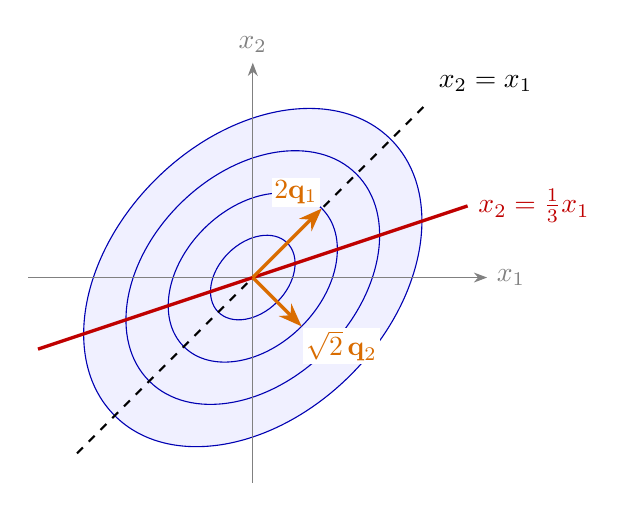
\begin{tikzpicture}[scale=0.62, >=Stealth]
        \fill[blue!6, rotate=45] (0,0) ellipse ({2*2} and {2*sqrt(2)});
        \foreach \r in {0.5,1,1.5,2}
            \draw[blue!70!black, rotate=45] (0,0) ellipse ({\r*2} and {\r*sqrt(2)});
        \draw[->, gray] (-4.6,0) -- (4.8,0) node[right] {$x_1$};
        \draw[->, gray] (0,-4.2) -- (0,4.4) node[above] {$x_2$};
        \draw[dashed, thick] (-3.6,-3.6) -- (3.6,3.6) node[above right] {$x_2 = x_1$};
        \draw[red!75!black, very thick] (-4.4,-4.4/3) -- (4.4,4.4/3) node[right] {$x_2 = \frac{1}{3}x_1$};
        \draw[->, very thick, orange!85!black] (0,0) -- (45:2) node[above left, fill=white, inner sep=1pt] {$2\mathbf{q}_1$};
        \draw[->, very thick, orange!85!black] (0,0) -- (-45:{sqrt(2)}) node[below right, fill=white, inner sep=1pt] {$\sqrt{2}\,\mathbf{q}_2$};
    \end{tikzpicture}
    \caption{Level curves of the density of $\mathcal{N}(\mathbf{0}, \Sigma)$ with $\Sigma = \left(\begin{smallmatrix} 3 & 1 \\ 1 & 3 \end{smallmatrix}\right)$, for Mahalanobis distances $r = 0.5, 1, 1.5, 2$. The eigenvectors $\mathbf{q}_1 = \frac{1}{\sqrt{2}}(1, 1)$ and $\mathbf{q}_2 = \frac{1}{\sqrt{2}}(1, -1)$ of $\Sigma$ have the eigenvalues $4$ and $2$, so the axes have half-lengths $2r$ and $\sqrt{2}\,r$ (orange: one standard deviation in each direction). The conditional mean $\E[X_2 \mid X_1 = x_1] = \frac{\Sigma_{21}}{\Sigma_{11}}x_1 = \frac{1}{3}x_1$ (red) is flatter than the major axis $x_2 = x_1$ (dashed).}
    \label{L4-fig:gaussian}
\end{figure}

\begin{corollary}\label{L4-cor:gaussian-linear}
    Let $\mathbf{X} \sim \mathcal{N}(\boldsymbol{\mu}, \Sigma)$, and let $A \in \mathbb{R}^{m \times d}$ have rank $m$. Then $A\mathbf{X} + \mathbf{b} \sim \mathcal{N}(A\boldsymbol{\mu} + \mathbf{b}, A\Sigma A^\top)$. In particular, if $X \sim \mathcal{N}(\mu_1, \sigma_1^2)$ and $Y \sim \mathcal{N}(\mu_2, \sigma_2^2)$ are independent, then $X + Y \sim \mathcal{N}(\mu_1 + \mu_2, \sigma_1^2 + \sigma_2^2)$.
\end{corollary}

\begin{proof}
    The rows of $A$ are linearly independent, so they can be extended to a basis of $\mathbb{R}^d$ (Lecture~1): there is a matrix $C$ such that $B = \left(\begin{smallmatrix} A \\ C \end{smallmatrix}\right)$ is invertible. Then $B\mathbf{X} + (\mathbf{b}, \mathbf{0})$ is Gaussian, and $A\mathbf{X} + \mathbf{b}$ is its first block, which is Gaussian by Theorem~\ref{L4-thm:gaussian-conditional}, with the mean and covariance of Proposition~\ref{L4-prop:covariance-matrix}. For the second statement, $(X, Y)$ is Gaussian with the covariance matrix $\diag(\sigma_1^2, \sigma_2^2)$ (its density is the product of the two densities), and $X + Y = (1, 1)(X, Y)^\top$.
\end{proof}

\section{Limit Theorems and Monte Carlo Methods}\label{L4-sec:limits}

Machine learning relies on averages: the training loss is an average over the data, a mini-batch gradient is an average over a few examples, and the test accuracy is an average over the test set. The limit theorems explain why averages of many random quantities are reliable.

\begin{proposition}\label{L4-prop:sample-mean}
    Let $X_1, \ldots, X_N$ be i.i.d.\ with mean $\mu$ and variance $\sigma^2$, and let $\bar X_N = \frac{1}{N}(X_1 + \cdots + X_N)$ be their sample mean. Then
    \[\E[\bar X_N] = \mu \qquad \text{and} \qquad \Var(\bar X_N) = \frac{\sigma^2}{N}.\]
\end{proposition}

\begin{proof}
    By linearity, $\E[\bar X_N] = \frac{1}{N} \cdot N\mu$, and by Proposition~\ref{L4-prop:variance-sum}, $\Var(\bar X_N) = \frac{1}{N^2} \cdot N\sigma^2$.
\end{proof}

So the standard deviation of the sample mean, its standard error, is $\frac{\sigma}{\sqrt{N}}$: to halve the error, we need four times as much data.

\begin{theorem}[Weak law of large numbers]\label{L4-thm:lln}
    In the situation of Proposition~\ref{L4-prop:sample-mean}, for every $\varepsilon > 0$,
    \[P(|\bar X_N - \mu| \geq \varepsilon) \leq \frac{\sigma^2}{N\varepsilon^2} \to 0 \qquad \text{as } N \to \infty.\]
\end{theorem}

\begin{proof}
    Chebyshev's inequality (Proposition~\ref{L4-prop:markov}) for $\bar X_N$, which has mean $\mu$ and variance $\frac{\sigma^2}{N}$.
\end{proof}

The law of large numbers says that the sample mean is very likely close to $\mu$ for large $N$. (The strong law of large numbers, Theorem~\ref{L4-thm:slln} below, even says that $\bar X_N \to \mu$ with probability $1$.) The central limit theorem describes the size and shape of the remaining fluctuations: they are approximately Gaussian, whatever the distribution of the $X_i$.

\begin{theorem}[Central limit theorem]\label{L4-thm:clt}
    In the situation of Proposition~\ref{L4-prop:sample-mean}, with $\sigma > 0$, for every $z \in \mathbb{R}$,
    \[P\Big(\frac{\sqrt{N}(\bar X_N - \mu)}{\sigma} \leq z\Big) \to \Phi(z) \qquad \text{as } N \to \infty.\]
\end{theorem}

We do not prove the central limit theorem. Informally, $\bar X_N$ is approximately $\mathcal{N}(\mu, \frac{\sigma^2}{N})$, and the sum $X_1 + \cdots + X_N$ is approximately $\mathcal{N}(N\mu, N\sigma^2)$. This explains why Gaussian distributions are so common: a measurement error that is the sum of many small independent effects is approximately Gaussian.

\begin{example}\label{L4-ex:clt-coins}
    We flip a fair coin $100$ times. The number of heads $S$ is Binomial$(100, \frac{1}{2})$, with mean $50$ and standard deviation $\sqrt{100 \cdot \frac{1}{4}} = 5$. By the central limit theorem, $P(S \geq 60) = P(S \geq 59.5) \approx 1 - \Phi\big(\frac{59.5 - 50}{5}\big) = 1 - \Phi(1.9) \approx 0.0287$, while the exact value is $0.0284$. (Replacing $60$ by $59.5$, the ``continuity correction'', improves the approximation of a discrete distribution by a continuous one.) Figure~\ref{L4-fig:clt} compares a binomial distribution with its Gaussian approximation.
\end{example}

\begin{figure}[ht]
    \centering
    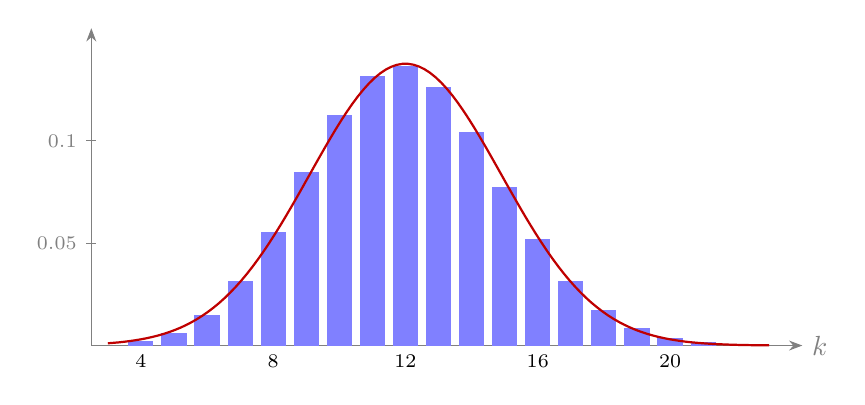
\begin{tikzpicture}[x=0.42cm, y=26cm, >=Stealth]
        \draw[->, gray] (2.5,0) -- (24,0) node[right] {$k$};
        \draw[->, gray] (2.5,0) -- (2.5,0.155);
        \foreach \k/\v in {4/0.0020, 5/0.0061, 6/0.0151, 7/0.0315, 8/0.0557, 9/0.0849, 10/0.1128, 11/0.1319, 12/0.1366, 13/0.1261, 14/0.1042, 15/0.0774, 16/0.0518, 17/0.0314, 18/0.0172, 19/0.0085, 20/0.0038, 21/0.0016}
            \fill[blue!50] (\k-0.38,0) rectangle (\k+0.38,\v);
        \draw[red!75!black, thick, domain=3:23, samples=120] plot (\x, {exp(-(\x-12)^2/(2*8.4))/sqrt(2*pi*8.4)});
        \foreach \k in {4,8,12,16,20}
            \node[below, font=\scriptsize] at (\k,0) {$\k$};
        \foreach \v in {0.05,0.1}
            \draw[gray] (2.35,\v) -- (2.65,\v) node[pos=0, left, font=\scriptsize] {$\v$};
    \end{tikzpicture}
    \caption{The pmf of the Binomial$(40, 0.3)$ distribution, the sum of $40$ independent Bernoulli$(0.3)$ variables, and the density of its Gaussian approximation $\mathcal{N}(12, 8.4)$ with the same mean and variance (red).}
    \label{L4-fig:clt}
\end{figure}

\paragraph{Monte Carlo estimation.} To compute an expectation $\E[g(X)]$ that we cannot compute exactly, we can draw i.i.d.\ samples $x_1, \ldots, x_N$ of $X$ and use the average $\frac{1}{N}\sum_i g(x_i)$. By the central limit theorem, its error is approximately Gaussian with standard deviation $\frac{\sigma_g}{\sqrt{N}}$, where $\sigma_g$ is the standard deviation of $g(X)$, no matter how high-dimensional $X$ is. For example, the fraction of $N$ uniformly random points of the square $[-1, 1]^2$ that land in the unit disk estimates $\frac{\pi}{4}$, so $4$ times this fraction estimates $\pi$, with standard error $4\sqrt{\frac{\pi}{4}(1 - \frac{\pi}{4})/N}$, which is $0.016$ for $N = 10\,000$. Each additional correct digit costs $100$ times more samples.

\paragraph{Concentration inequalities.} The central limit theorem is only an approximation for finite $N$. For bounded random variables, there is an exact bound that is much stronger than Chebyshev's inequality.

\begin{theorem}[Hoeffding's inequality]\label{L4-thm:hoeffding}
    Let $X_1, \ldots, X_N$ be i.i.d.\ with mean $\mu$ and values in $[a, b]$. Then for every $\varepsilon > 0$,
    \[P(|\bar X_N - \mu| \geq \varepsilon) \leq 2\exp\Big(-\frac{2N\varepsilon^2}{(b - a)^2}\Big).\]
\end{theorem}

We do not prove this theorem. For example, let a classifier have the (unknown) error rate $\mu$, and let $\bar X_N$ be its error rate on a test set of $N = 1000$ examples drawn independently of the training data, where $X_i \in \{0, 1\}$ indicates an error. Then $P(|\bar X_N - \mu| \geq 0.05) \leq 2e^{-5} \approx 0.013$, while Chebyshev's inequality with $\sigma^2 \leq \frac{1}{4}$ only gives $0.1$.

\begin{remark}[Limit theorems in machine learning]
    \begin{enumerate}
        \item The average loss on the training data, $\frac{1}{N}\sum_i \ell(\boldsymbol{\theta}; \mathbf{x}_i, y_i)$, is a sample mean. It estimates the expected loss $\E[\ell(\boldsymbol{\theta}; \mathbf{X}, Y)]$ on new data, which is the quantity we actually care about. For a fixed $\boldsymbol{\theta}$, the limit theorems apply. But the trained parameters depend on the training data, so the training loss of the trained model is a biased, usually too optimistic, estimate (overfitting). This is why we evaluate on separate test data, and why learning theory combines Hoeffding's inequality with the union bound (Proposition~\ref{L4-prop:probability-rules}) to control all candidate models simultaneously.
        \item In stochastic gradient descent (Lecture~3), the mini-batch gradient of $B$ randomly chosen examples is an unbiased estimate of the full gradient, and its covariance matrix decreases like $\frac{1}{B}$ (for sampling with replacement), by Proposition~\ref{L4-prop:sample-mean} applied to each coordinate. Larger batches give less noisy gradients, but each step costs more.
    \end{enumerate}
\end{remark}

\subsection{Modes of convergence and the strong law}\label{L4-sec:convergence}

The weak law of large numbers is a statement about probabilities, for each $N$. Measure theory allows statements about the whole random sequence: for example, that $\bar X_N(\omega) \to \mu$ for almost every outcome $\omega$, i.e., along almost every infinite sequence of observations. Random variables can converge in several different senses.

\begin{definition}[Modes of convergence]\label{L4-def:convergence-modes}
    Let $X, X_1, X_2, \ldots$ be random variables on the same probability space. We say that $X_n \to X$
    \begin{enumerate}
        \item almost surely if $P(X_n \to X) = 1$, i.e., $X_n(\omega) \to X(\omega)$ for all $\omega$ outside a null set;
        \item in probability if $P(|X_n - X| > \varepsilon) \to 0$ for every $\varepsilon > 0$;
        \item in $L^p$, for $p \geq 1$, if $\E[|X_n - X|^p] \to 0$; for $p = 2$, this is convergence in mean square.
    \end{enumerate}
    Random variables $X_n$ and $X$, possibly on different probability spaces, converge in distribution if $F_{X_n}(x) \to F_X(x)$ at every point $x$ at which $F_X$ is continuous.
\end{definition}

The weak law of large numbers (Theorem~\ref{L4-thm:lln}) is convergence in probability, and the central limit theorem (Theorem~\ref{L4-thm:clt}) is convergence in distribution of the standardized means to $\mathcal{N}(0, 1)$.

\begin{proposition}\label{L4-prop:convergence-modes}
    Almost sure convergence and convergence in $L^p$ each imply convergence in probability, which implies convergence in distribution. None of the converse implications holds in general.
\end{proposition}

\begin{proof}[Proof of some parts]
    If $X_n \to X$ almost surely, the events $A_n = \{|X_m - X| > \varepsilon \text{ for some } m \geq n\}$ decrease to an event that is contained in the null event $\{X_n \not\to X\}$, so $P(|X_n - X| > \varepsilon) \leq P(A_n) \to 0$ by continuity. Convergence in $L^p$ implies convergence in probability by Markov's inequality: $P(|X_n - X| > \varepsilon) \leq \frac{\E[|X_n - X|^p]}{\varepsilon^p}$. We omit the proof of the last implication; Example~\ref{L4-ex:convergence-counterexamples} disproves the converses.
\end{proof}

\begin{example}\label{L4-ex:convergence-counterexamples}
    Let $U$ be uniform on $[0, 1)$.
    \begin{enumerate}
        \item The lottery tickets $X_n = n\mathbf{1}_{\{U < 1/n\}}$ of Example~\ref{L4-ex:escaping-mass} converge to $0$ almost surely, since $X_n = 0$ as soon as $n > \frac{1}{U}$, but not in $L^1$, since $\E[X_n] = 1$.
        \item (A sliding block.) Write $n = 2^k + j$ with $0 \leq j < 2^k$, and let $X_n = \mathbf{1}_{\{j2^{-k} \leq U < (j + 1)2^{-k}\}}$: the indicator of a block of length $2^{-k}$, which slides across $[0, 1)$, and then starts again with half the length. Then $\E[|X_n|^p] = 2^{-k} \to 0$, so $X_n \to 0$ in every $L^p$ and in probability. But for every value of $U$, one block of every generation $k$ covers it, so $X_n = 1$ for infinitely many $n$, and the sequence $X_n(\omega)$ converges for no outcome $\omega$.
        \item If $X \sim \mathcal{N}(0, 1)$ and $X_n = -X$ for all $n$, then $X_n \to X$ in distribution, since $-X$ has the same distribution as $X$, but $|X_n - X| = 2|X|$ does not converge to $0$ in probability.
    \end{enumerate}
\end{example}

The main tool for proving almost sure convergence is the following lemma.

\begin{lemma}[Borel--Cantelli]\label{L4-lem:borel-cantelli}
    Let $A_1, A_2, \ldots$ be events, and let $\{A_n \text{ i.o.}\}$ be the event that infinitely many of them happen (``infinitely often'').
    \begin{enumerate}
        \item If $\sum_n P(A_n) < \infty$, then $P(A_n \text{ i.o.}) = 0$.
        \item If the $A_n$ are independent and $\sum_n P(A_n) = \infty$, then $P(A_n \text{ i.o.}) = 1$.
    \end{enumerate}
\end{lemma}

\begin{proof}
    (1) For every $k$, $\{A_n \text{ i.o.}\} \subseteq \bigcup_{n \geq k} A_n$, which has probability at most $\sum_{n \geq k} P(A_n)$ by the union bound, and this tends to $0$ as $k \to \infty$. (2) The complement of $\{A_n \text{ i.o.}\}$ is the union over $k$ of the events $\bigcap_{n \geq k} A_n^c$. By independence and $1 - x \leq e^{-x}$, for all $m \geq k$,
    \[P\Big(\bigcap_{n=k}^m A_n^c\Big) = \prod_{n=k}^m \big(1 - P(A_n)\big) \leq \exp\Big(-\sum_{n=k}^m P(A_n)\Big),\]
    which tends to $0$ as $m \to \infty$. So every $\bigcap_{n \geq k} A_n^c$ is a null event, and so is their countable union.
\end{proof}

\begin{example}\label{L4-ex:borel-cantelli}
    Consider infinitely many fair coin flips (Example~\ref{L4-ex:coin-flips}). The events $A_k$ that the flips $2k - 1$ and $2k$ are both heads are independent and have the probability $\frac{1}{4}$, so by part (2), almost surely, two heads in a row appear infinitely often; the same argument works for every finite pattern, for example for the text of this lecture, encoded in bits. On the other hand, let $B_k$ be the event that the $\lceil 2\log_2 k\rceil$ flips starting with flip $k$ are all heads. Then $P(B_k) \leq k^{-2}$, which is summable, so by part (1), almost surely, only finitely many $B_k$ happen: the longest run of heads among the first $n$ flips is eventually shorter than about $2\log_2 n$.
\end{example}

\begin{theorem}[Strong law of large numbers]\label{L4-thm:slln}
    Let $X_1, X_2, \ldots$ be i.i.d.\ and integrable with mean $\mu$. Then $\bar X_N \to \mu$ almost surely.
\end{theorem}

\begin{proof}[Proof if $X_1$ has a finite fourth moment]
    Let $Y_i = X_i - \mu$ and $S_N = Y_1 + \cdots + Y_N$. When we expand $S_N^4 = \sum_{i, j, k, l} Y_iY_jY_kY_l$, every term in which some $Y_i$ appears exactly once has expectation $0$, by independence. What remains are the $N$ terms $Y_i^4$ and the $3N(N - 1)$ terms $Y_i^2Y_j^2$ with $i \neq j$, so $\E[S_N^4] = N\E[Y_1^4] + 3N(N - 1)\sigma^4 \leq CN^2$ for a constant $C$. By Markov's inequality,
    \[P(|\bar X_N - \mu| \geq \varepsilon) = P(S_N^4 \geq N^4\varepsilon^4) \leq \frac{C}{N^2\varepsilon^4},\]
    which is summable. By the Borel--Cantelli lemma, almost surely, $|\bar X_N - \mu| \geq \varepsilon$ only for finitely many $N$. Applying this to $\varepsilon = \frac{1}{m}$ for $m = 1, 2, \ldots$ (countably many null events) gives $\bar X_N \to \mu$ almost surely.
\end{proof}

\begin{example}[Normal numbers]\label{L4-ex:normal-numbers}
    The binary digits of a uniformly random $U \in [0, 1)$ are i.i.d.\ fair coin flips (Example~\ref{L4-ex:coin-flips}). By the strong law, the fraction of $1$s among the first $N$ digits converges to $\frac{1}{2}$ almost surely: almost every number in $[0, 1)$ has asymptotically equally many $0$s and $1$s in its binary expansion (Borel's normal number theorem, 1909). Yet for natural constants such as $\sqrt{2} - 1$, it is not known whether they have this property. This is typical of probabilistic arguments: they show that almost all objects have a property, without exhibiting one.
\end{example}

\paragraph{Convergence in distribution.} Two rules allow us to combine limits in distribution.

\begin{theorem}[Continuous mapping and Slutsky]\label{L4-thm:slutsky}
    Let $X_n \to X$ in distribution.
    \begin{enumerate}
        \item If $g$ is continuous, then $g(X_n) \to g(X)$ in distribution.
        \item (Slutsky) If $Y_n \to c$ in probability for a constant $c$, then $X_n + Y_n \to X + c$ and $X_nY_n \to cX$ in distribution.
    \end{enumerate}
\end{theorem}

We do not prove this theorem. It justifies the confidence intervals of Section~\ref{L4-sec:estimation}, in which we replace $\sigma$ by the sample standard deviation $s_N$. By the strong law, applied to the $X_i$ and the $X_i^2$, $s_N \to \sigma$ almost surely, so by Slutsky's theorem,
\[\frac{\sqrt{N}(\bar X_N - \mu)}{s_N} = \frac{\sigma}{s_N} \cdot \frac{\sqrt{N}(\bar X_N - \mu)}{\sigma} \to \mathcal{N}(0, 1) \qquad \text{in distribution},\]
and $\bar x \pm 1.96\frac{s}{\sqrt{N}}$ is an asymptotic $95\%$ confidence interval.

\begin{proposition}[Delta method]\label{L4-prop:delta-method}
    Let $\sqrt{N}(T_N - \theta) \to \mathcal{N}(0, \tau^2)$ in distribution, and let $g$ be continuously differentiable. Then $\sqrt{N}\big(g(T_N) - g(\theta)\big) \to \mathcal{N}\big(0, g'(\theta)^2\tau^2\big)$ in distribution.
\end{proposition}

\begin{proof}[Sketch of proof]
    By the mean value theorem, $g(T_N) - g(\theta) = g'(\xi_N)(T_N - \theta)$ for some $\xi_N$ between $\theta$ and $T_N$. Since $T_N - \theta = \frac{1}{\sqrt{N}} \cdot \sqrt{N}(T_N - \theta) \to 0$ in probability (by Slutsky's theorem), $\xi_N \to \theta$ and $g'(\xi_N) \to g'(\theta)$ in probability. Now apply Slutsky's theorem to $g'(\xi_N) \cdot \sqrt{N}(T_N - \theta)$.
\end{proof}

\begin{example}[Confidence intervals on the log-odds scale]\label{L4-ex:delta}
    For a proportion $\hat p = \bar X_N$ of $N$ Bernoulli$(p)$ observations, $\sqrt{N}(\hat p - p) \to \mathcal{N}(0, p(1 - p))$ by the central limit theorem. The log-odds $g(p) = \log\frac{p}{1 - p}$ have the derivative $g'(p) = \frac{1}{p(1 - p)}$, so the estimated log-odds $g(\hat p)$ have approximately the standard error $\frac{1}{\sqrt{Np(1 - p)}}$. For $30$ successes in $100$ trials, the log-odds are $\log\frac{0.3}{0.7} \approx -0.847$, with the estimated standard error $\frac{1}{\sqrt{21}} \approx 0.218$. This gives the approximate $95\%$ confidence interval $-0.847 \pm 1.96 \cdot 0.218 \approx [-1.275, -0.420]$ for the log-odds, and, transforming back with the sigmoid function, $[0.218, 0.397]$ for $p$. Unlike the interval $\hat p \pm 1.96\sqrt{\hat p(1 - \hat p)/N} = [0.210, 0.390]$, it is not symmetric around $\hat p$, and it never leaves $[0, 1]$. Logistic regression (Lecture~3) models the log-odds, and its standard errors are computed on this scale.
\end{example}

\subsection{Monte Carlo sampling}\label{L4-sec:monte-carlo}

Monte Carlo estimation needs samples from the distribution of interest. We have already seen inverse transform sampling (Theorem~\ref{L4-thm:inverse-transform}) and sampling Gaussian vectors by affine maps (Section~\ref{L4-sec:gaussian}), and we will see Markov chain Monte Carlo in Section~\ref{L4-sec:markov}. Two further general methods are rejection sampling, which produces exact samples, and importance sampling, which reweights samples from a different distribution.

\begin{theorem}[Rejection sampling]\label{L4-thm:rejection}
    Let $p$ and $q$ be densities, and let $M \geq 1$ be such that $p(x) \leq Mq(x)$ for all $x$. Repeat the following trial until a value is accepted: draw $X \sim q$ and, independently, $U \sim$ Uniform$(0, 1)$, and accept $X$ if $U \leq \frac{p(X)}{Mq(X)}$. Then the accepted value has the density $p$, and each trial is accepted with probability $\frac{1}{M}$.
\end{theorem}

\begin{proof}
    For every set $A$, $P(X \in A \text{ and accepted}) = \int_A q(x)\,\frac{p(x)}{Mq(x)}\, dx = \frac{1}{M}\int_A p(x)\, dx$. For $A = \mathbb{R}$, this gives $P(\text{accepted}) = \frac{1}{M}$, so $P(X \in A \mid \text{accepted}) = \int_A p(x)\, dx$. Since the trials are independent, the accepted value has this conditional distribution.
\end{proof}

Geometrically, the points $(X, UMq(X))$ are uniformly distributed under the graph of $Mq$, and we keep those that lie under the graph of $p$; their first coordinates have the density $p$. The method also works if $p$ is only known up to a constant. For example, the Beta$(2, 2)$ density $6x(1 - x)$ is at most $1.5$ on $[0, 1]$, so with the uniform proposal and $M = 1.5$, two out of three trials are accepted. In high dimensions, however, $M$ is usually enormous: for the target $\mathcal{N}(\mathbf{0}, I)$ in $\mathbb{R}^d$ and the proposal $\mathcal{N}(\mathbf{0}, 2I)$, the ratio $\frac{p}{q} = 2^{d/2}e^{-\norm{\mathbf{x}}^2/4}$ forces $M \geq 2^{d/2}$, so only one in $1024$ trials is accepted for $d = 20$. This is one reason why high-dimensional sampling relies on MCMC.

\begin{proposition}[Importance sampling]\label{L4-prop:importance}
    Let $p$ and $q$ be densities such that $q(x) > 0$ for all $x$ with $f(x)p(x) \neq 0$, and let $w = \frac{p}{q}$ (the importance weights). Then $\E_p[f(X)] = \E_q[f(Y)w(Y)]$. Hence, for i.i.d.\ samples $y_1, \ldots, y_N$ from $q$, the estimator
    \[\hat I = \frac{1}{N}\sum_{i=1}^N f(y_i)w(y_i)\]
    is unbiased, with variance $\frac{1}{N}\Var_q(f(Y)w(Y))$.
\end{proposition}

\begin{proof}
    $\int f(x)p(x)\, dx = \int f(y)\frac{p(y)}{q(y)}q(y)\, dy$; the variance follows from Proposition~\ref{L4-prop:sample-mean}.
\end{proof}

The variance is small if $q$ puts its mass where $|f|p$ is large; for $f \geq 0$, the ideal (but impractical) choice $q \propto fp$ even gives variance $0$.

\begin{example}[A rare event]\label{L4-ex:importance}
    The tail probability $P(Z > 4) = 3.17 \cdot 10^{-5}$ of $Z \sim \mathcal{N}(0, 1)$ is hard to estimate by plain Monte Carlo: among $N = 10\,000$ samples, we expect only $0.32$ samples above $4$, and the relative standard error of the estimate is about $178\%$. With the proposal $q = \mathcal{N}(4, 1)$, about half of the samples land above $4$, and they are reweighted by $w(y) = \frac{\varphi(y)}{\varphi(y - 4)} = e^{8 - 4y}$. With the same $N$, the relative standard error drops to about $2\%$. Probabilities of rare failures are estimated in this way.
\end{example}

If $p$ is only known up to a constant, one uses the self-normalized estimator $\sum_i f(y_i)w_i / \sum_i w_i$, which is slightly biased but consistent. If a few weights dominate, the estimate is unreliable; the effective sample size $\frac{(\sum_i w_i)^2}{\sum_i w_i^2}$ measures how many samples effectively contribute. In machine learning, importance weights correct for differences between distributions: in off-policy evaluation in reinforcement learning (data collected with one policy, used to evaluate another), and under covariate shift, where training examples are weighted by the ratio of the test and training densities.

\section{Markov Chains}\label{L4-sec:markov}

So far, we mostly considered independent random variables. Many random sequences have memory: tomorrow's weather depends on today's, the next word of a sentence depends on the previous ones, and a user browsing the web chooses the next page depending on the current one. The simplest model with memory is a Markov chain, in which the future depends on the past only through the present.

\begin{definition}[Markov chain]\label{L4-def:markov}
    A sequence of random variables $X_0, X_1, X_2, \ldots$ with values in a finite set of states $\{1, \ldots, n\}$ is a Markov chain with transition matrix $P \in \mathbb{R}^{n \times n}$ if
    \[P(X_{t+1} = j \mid X_t = i, X_{t-1} = i_{t-1}, \ldots, X_0 = i_0) = P_{ij}\]
    for all times $t$ and all states $i, j, i_0, \ldots, i_{t-1}$ (whenever the condition has positive probability).
\end{definition}

The entry $P_{ij}$ is the probability of moving from state $i$ to state $j$ in one step. So $P$ has nonnegative entries, and each row sums to $1$, i.e., $P\mathbf{1} = \mathbf{1}$; such matrices are called stochastic matrices.

\begin{example}[Weather]\label{L4-ex:weather}
    Let state $1$ be ``sunny'' and state $2$ ``rainy''. After a sunny day, the next day is sunny with probability $0.9$; after a rainy day, it is sunny with probability $0.5$:
    \[P = \begin{pmatrix} 0.9 & 0.1 \\ 0.5 & 0.5 \end{pmatrix}.\]
    The chain is drawn as a graph with an arrow $i \to j$ labeled $P_{ij}$ for each possible transition (Figure~\ref{L4-fig:markov}).
\end{example}

We write the distribution of $X_t$ as a row vector $\boldsymbol{\pi}_t = \big(P(X_t = 1), \ldots, P(X_t = n)\big)$. (The same weather model appears in the section on eigenvalues in Lecture~1, with the distributions written as columns and multiplied by the transposed matrix $P^\top$.)

\begin{proposition}\label{L4-prop:markov-evolution}
    $\boldsymbol{\pi}_{t+1} = \boldsymbol{\pi}_t P$, hence $\boldsymbol{\pi}_t = \boldsymbol{\pi}_0 P^t$. More generally, $P(X_{t+k} = j \mid X_t = i) = (P^k)_{ij}$.
\end{proposition}

\begin{proof}
    By the law of total probability (Theorem~\ref{L4-thm:bayes}), $P(X_{t+1} = j) = \sum_i P(X_t = i)\,P(X_{t+1} = j \mid X_t = i) = \sum_i (\boldsymbol{\pi}_t)_i P_{ij}$. The second statement follows by induction on $k$, in the same way.
\end{proof}

So the distribution evolves by repeated multiplication with $P$, and the long-term behavior of the chain is a question about the powers of a matrix, i.e., about its eigenvalues (Lecture~1). For the weather chain, starting on a sunny day, $\boldsymbol{\pi}_0 = (1, 0)$, $\boldsymbol{\pi}_1 = (0.9, 0.1)$, $\boldsymbol{\pi}_2 = (0.86, 0.14)$, $\boldsymbol{\pi}_3 = (0.844, 0.156)$, and the distribution seems to approach a limit.

\begin{definition}[Stationary distribution]\label{L4-def:stationary}
    A probability distribution $\boldsymbol{\pi}$ (a row vector with $\pi_i \geq 0$ and $\sum_i \pi_i = 1$) is stationary for $P$ if $\boldsymbol{\pi}P = \boldsymbol{\pi}$.
\end{definition}

If $X_0$ has a stationary distribution, then so does every $X_t$. Transposing, $P^\top\boldsymbol{\pi}^\top = \boldsymbol{\pi}^\top$: a stationary distribution is an eigenvector of $P^\top$ with the eigenvalue $1$ (a left eigenvector of $P$), scaled to have entries that sum to $1$.

\begin{proposition}\label{L4-prop:stochastic-eigenvalues}
    Let $P$ be a stochastic matrix. Then $1$ is an eigenvalue of $P$ and of $P^\top$, and every (complex) eigenvalue $\lambda$ of $P$ satisfies $|\lambda| \leq 1$.
\end{proposition}

\begin{proof}
    $P\mathbf{1} = \mathbf{1}$, and $P^\top$ has the same characteristic polynomial as $P$, since $\det(A^\top) = \det(A)$ (Lecture~1). If $P\mathbf{v} = \lambda\mathbf{v}$ with $\mathbf{v} \neq \mathbf{0}$, choose $i$ with $|v_i| = \max_j |v_j|$. Then $|\lambda||v_i| = |\sum_j P_{ij}v_j| \leq \sum_j P_{ij}|v_j| \leq \sum_j P_{ij}|v_i| = |v_i|$.
\end{proof}

Whether the distribution converges to a stationary distribution depends on two properties. A chain is irreducible if every state can be reached from every other state, i.e., for all $i$ and $j$ there is a $t$ with $(P^t)_{ij} > 0$. It is aperiodic if for every state $i$, the numbers $t \geq 1$ with $(P^t)_{ii} > 0$ have greatest common divisor $1$; for an irreducible chain, it suffices that some $P_{ii} > 0$.

\begin{theorem}[Convergence of Markov chains]\label{L4-thm:markov-convergence}
    An irreducible Markov chain has a unique stationary distribution $\boldsymbol{\pi}$, and all $\pi_i > 0$. If the chain is also aperiodic, then $\boldsymbol{\pi}_0 P^t \to \boldsymbol{\pi}$ as $t \to \infty$, for every initial distribution $\boldsymbol{\pi}_0$.
\end{theorem}

We do not prove this theorem in general; it is a consequence of the Perron--Frobenius theorem on matrices with nonnegative entries. The speed of convergence is governed by the second largest absolute value of an eigenvalue of $P$. Both assumptions are needed. For $P = \left(\begin{smallmatrix} 0 & 1 \\ 1 & 0 \end{smallmatrix}\right)$, the chain alternates between the two states: $(\frac{1}{2}, \frac{1}{2})$ is stationary, but $\boldsymbol{\pi}_0 = (1, 0)$ gives $\boldsymbol{\pi}_t = (1, 0), (0, 1), (1, 0), \ldots$ (the chain has period $2$, and $-1$ is an eigenvalue). For $P = I$, the chain never moves, and every distribution is stationary. For two states, everything can be computed by hand.

\begin{proposition}[Two-state chains]\label{L4-prop:two-state}
    Let $P = \begin{pmatrix} 1 - a & a \\ b & 1 - b \end{pmatrix}$ with $a + b > 0$. Then $\boldsymbol{\pi} = \big(\frac{b}{a + b}, \frac{a}{a + b}\big)$ is stationary, and for every initial distribution,
    \[\boldsymbol{\pi}_t - \boldsymbol{\pi} = (1 - a - b)^t\,(\boldsymbol{\pi}_0 - \boldsymbol{\pi}).\]
\end{proposition}

\begin{proof}
    One checks $\boldsymbol{\pi}P = \boldsymbol{\pi}$ directly. The difference $\mathbf{d} = \boldsymbol{\pi}_0 - \boldsymbol{\pi}$ has entries that sum to $0$, so $\mathbf{d} = c(1, -1)$, and $(1, -1)P = (1 - a - b, \, a - 1 + b) = (1 - a - b)(1, -1)$: the row vector $(1, -1)$ is a left eigenvector with the eigenvalue $1 - a - b$. Hence $\boldsymbol{\pi}_t - \boldsymbol{\pi} = (\boldsymbol{\pi}_0 - \boldsymbol{\pi})P^t = (1 - a - b)^t\,\mathbf{d}$.
\end{proof}

For the weather chain, $a = 0.1$ and $b = 0.5$, so the stationary distribution is $(\frac{5}{6}, \frac{1}{6})$, and the distance to it shrinks by the factor $0.4$ (the second eigenvalue of $P$) every day. Starting on a sunny day, $P(X_t = \text{sunny}) = \frac{5}{6} + \frac{1}{6}\,0.4^t$; starting on a rainy day, it is $\frac{5}{6} - \frac{5}{6}\,0.4^t$ (Figure~\ref{L4-fig:markov}).

\begin{figure}[ht]
    \centering
    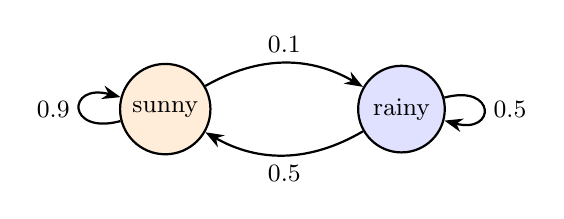
\begin{tikzpicture}[>=Stealth, every node/.style={font=\small}]
        \node[circle, draw, thick, fill=orange!15, minimum size=1.1cm] (S) at (0,0) {sunny};
        \node[circle, draw, thick, fill=blue!12, minimum size=1.1cm] (R) at (3,0) {rainy};
        \draw[->, thick] (S) to[bend left=30] node[above] {$0.1$} (R);
        \draw[->, thick] (R) to[bend left=30] node[below] {$0.5$} (S);
        \draw[->, thick] (S) to[loop left, looseness=6] node[left] {$0.9$} (S);
        \draw[->, thick] (R) to[loop right, looseness=6] node[right] {$0.5$} (R);
    \end{tikzpicture}
    \qquad
    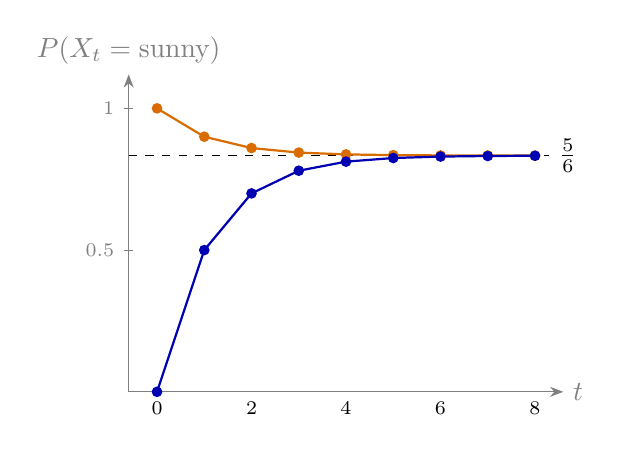
\begin{tikzpicture}[x=0.6cm, y=3.6cm, >=Stealth]
        \draw[->, gray] (-0.6,0) -- (8.6,0) node[right] {$t$};
        \draw[->, gray] (-0.6,0) -- (-0.6,1.12) node[above] {$P(X_t = \text{sunny})$};
        \draw[dashed] (-0.6,{5/6}) -- (8.3,{5/6}) node[right] {$\frac{5}{6}$};
        \draw[orange!85!black, thick] plot[domain=0:8, samples=9, mark=*, mark size=1.5pt] (\x, {5/6 + (1/6)*0.4^\x});
        \draw[blue!70!black, thick] plot[domain=0:8, samples=9, mark=*, mark size=1.5pt] (\x, {5/6 - (5/6)*0.4^\x});
        \foreach \t in {0,2,4,6,8}
            \node[below, font=\scriptsize] at (\t,0) {$\t$};
        \foreach \v in {0.5,1}
            \draw[gray] (-0.5,\v) -- (-0.7,\v) node[left, font=\scriptsize] {$\v$};
    \end{tikzpicture}
    \caption{Left: the weather chain of Example~\ref{L4-ex:weather}. Right: the probability of a sunny day $t$ days after a sunny day (orange) and after a rainy day (blue); both converge to the stationary probability $\frac{5}{6}$, and the distance shrinks by the factor $0.4$ every day.}
    \label{L4-fig:markov}
\end{figure}

\paragraph{The ergodic theorem.} For an irreducible chain, the fraction of time that the chain spends in state $i$ converges to $\pi_i$ with probability $1$, and more generally $\frac{1}{T}\sum_{t=0}^{T-1} f(X_t) \to \sum_i \pi_i f(i)$ for every function $f$. This is a law of large numbers for dependent random variables, which we state without proof. In the long run, $\frac{5}{6}$ of the days are sunny. Since successive states are correlated, these averages converge more slowly than averages of independent samples.

\subsection{Detailed balance and Markov chain Monte Carlo}

Finding a stationary distribution means solving a linear system. It is often easier to check a stronger, local condition.

\begin{proposition}[Detailed balance]\label{L4-prop:detailed-balance}
    If a distribution $\boldsymbol{\pi}$ satisfies $\pi_i P_{ij} = \pi_j P_{ji}$ for all states $i$ and $j$, then it is stationary.
\end{proposition}

\begin{proof}
    $(\boldsymbol{\pi}P)_j = \sum_i \pi_i P_{ij} = \sum_i \pi_j P_{ji} = \pi_j\sum_i P_{ji} = \pi_j$.
\end{proof}

Detailed balance says that in the stationary regime, the probability flow from $i$ to $j$ equals the flow from $j$ to $i$; such chains are called reversible.

\begin{example}[Random walks on graphs]\label{L4-ex:random-walk-graph}
    Let $G$ be a connected undirected graph, and let a walker move from each vertex to a uniformly random neighbor, i.e., $P_{ij} = \frac{1}{\deg(i)}$ for each edge $\{i, j\}$. Then $\pi_i = \frac{\deg(i)}{2|E|}$, where $|E|$ is the number of edges, satisfies detailed balance: $\pi_i P_{ij} = \frac{1}{2|E|} = \pi_j P_{ji}$ for every edge. So in the long run, the walker visits each vertex in proportion to its degree. For the graph with the edges $\{1, 2\}$, $\{1, 3\}$, $\{2, 3\}$, $\{3, 4\}$, the degrees are $2, 2, 3, 1$, and $\boldsymbol{\pi} = (\frac{1}{4}, \frac{1}{4}, \frac{3}{8}, \frac{1}{8})$.
\end{example}

\begin{remark}[PageRank]
    Google's original PageRank models a ``random surfer'' who, at each step, follows a uniformly random link on the current page with probability $\alpha$ (typically $0.85$), and jumps to a uniformly random page with probability $1 - \alpha$. All entries of the resulting transition matrix are positive, so the chain is irreducible and aperiodic, and its unique stationary distribution ranks the pages. It is computed by the power iteration $\boldsymbol{\pi} \leftarrow \boldsymbol{\pi}P$ of the programming exercises of Lecture~1.
\end{remark}

Detailed balance is also the key to Markov chain Monte Carlo (MCMC), the most important method for sampling from complicated distributions, such as the posterior distributions of Section~\ref{L4-sec:bayesian}. These are often only known up to a constant: $p(\theta \mid \mathcal{D}) \propto p(\mathcal{D} \mid \theta)\,p(\theta)$, where the evidence $p(\mathcal{D})$ is an intractable integral. The idea is to construct a Markov chain whose stationary distribution is the target distribution, run it for a long time, and use its states as (dependent) samples.

\begin{theorem}[Metropolis algorithm]\label{L4-thm:metropolis}
    Let $\boldsymbol{\pi}$ be a distribution with all $\pi_i > 0$, and let $Q$ be a symmetric stochastic matrix ($Q_{ij} = Q_{ji}$), the proposal. From the state $i$, propose a state $j$ with probability $Q_{ij}$, and move to $j$ with the acceptance probability $\min\big(1, \frac{\pi_j}{\pi_i}\big)$; otherwise, stay at $i$. This defines a Markov chain that satisfies detailed balance with respect to $\boldsymbol{\pi}$, so $\boldsymbol{\pi}$ is stationary.
\end{theorem}

\begin{proof}
    For $i \neq j$, $P_{ij} = Q_{ij}\min\big(1, \frac{\pi_j}{\pi_i}\big)$, so $\pi_i P_{ij} = Q_{ij}\min(\pi_i, \pi_j)$, which is symmetric in $i$ and $j$ because $Q$ is. For $i = j$, detailed balance holds trivially.
\end{proof}

The algorithm only uses the ratios $\frac{\pi_j}{\pi_i}$, so the unknown normalizing constant cancels. Moves to more probable states are always accepted, and moves to less probable states sometimes. For densities, the same algorithm works with a symmetric proposal such as $\theta' = \theta + \eta\,\varepsilon$ with $\varepsilon \sim \mathcal{N}(0, 1)$, and the ratio of the (unnormalized) densities. If the resulting chain is irreducible and aperiodic, Theorem~\ref{L4-thm:markov-convergence} and the ergodic theorem justify using averages along the chain as estimates of expectations under $\boldsymbol{\pi}$.

\begin{example}\label{L4-ex:metropolis}
    Let the states $1, 2, 3, 4$ lie on a cycle, let $Q$ propose each of the two neighbors with probability $\frac{1}{2}$, and let the target be $\boldsymbol{\pi} = (0.1, 0.2, 0.3, 0.4)$. The Metropolis chain has the transition matrix
    \[P = \begin{pmatrix} 0 & 0.5 & 0 & 0.5 \\ 0.25 & 0.25 & 0.5 & 0 \\ 0 & 1/3 & 1/6 & 0.5 \\ 0.125 & 0 & 0.375 & 0.5 \end{pmatrix};\]
    for example, from state $3$, the move to state $2$ is proposed with probability $\frac{1}{2}$ and accepted with probability $\frac{0.2}{0.3}$, so $P_{32} = \frac{1}{3}$. One checks that $\boldsymbol{\pi}P = \boldsymbol{\pi}$.
\end{example}

\begin{remark}[Markov models in machine learning]
    An $n$-gram language model is a Markov chain on words (or on tuples of $n - 1$ words), whose transition probabilities are estimated by counting in a large text, which is maximum likelihood estimation (Section~\ref{L4-sec:estimation}). Hidden Markov models, in which only a noisy function of the state is observed, were long the standard model in speech recognition. Reinforcement learning is based on Markov decision processes, in which the transition probabilities depend on the actions of an agent. Diffusion models for image generation learn to reverse a Markov chain that gradually adds Gaussian noise to an image (Section~\ref{L4-sec:langevin}).
\end{remark}

\section{Parameter Estimation}\label{L4-sec:estimation}

Statistics turns the questions of probability around: instead of computing probabilities from a known distribution, we infer an unknown distribution from data. We assume that the data $x_1, \ldots, x_N$ are i.i.d.\ samples from a distribution $p(x \mid \theta)$ that belongs to a known family, with an unknown parameter $\theta$ (for example, the mean and variance of a Gaussian, or the weights of a model).

\begin{definition}[Estimator, bias and variance]\label{L4-def:estimator}
    An estimator is a function $\hat\theta = \hat\theta(X_1, \ldots, X_N)$ of the data; as a function of random data, it is a random variable. Its bias is $\E[\hat\theta] - \theta$, and it is unbiased if the bias is $0$ for all $\theta$. Its mean squared error is $\mathrm{MSE}(\hat\theta) = \E[(\hat\theta - \theta)^2]$.
\end{definition}

\begin{proposition}[Bias--variance decomposition]\label{L4-prop:bias-variance}
    $\mathrm{MSE}(\hat\theta) = \big(\E[\hat\theta] - \theta\big)^2 + \Var(\hat\theta)$.
\end{proposition}

\begin{proof}
    Let $m = \E[\hat\theta]$. Then $\E[(\hat\theta - \theta)^2] = \E[(\hat\theta - m)^2] + 2(m - \theta)\E[\hat\theta - m] + (m - \theta)^2$, and the middle term is $0$.
\end{proof}

A good estimator has a small bias and a small variance, and sometimes we accept some bias for a much smaller variance. This is the idea behind regularization: ridge regression shrinks the weights towards $0$, which introduces a bias but reduces the variance. For a prediction model, a similar decomposition says that the expected squared test error is the sum of the squared bias, the variance and the irreducible noise; very flexible models have a small bias but a large variance (they overfit), and very simple ones the opposite.

\begin{example}[Shrinkage]\label{L4-ex:shrinkage}
    Let $X_1, \ldots, X_N$ be i.i.d.\ $\mathcal{N}(\mu, \sigma^2)$, and consider the estimators $\hat\mu_c = c\bar X_N$ with $0 \leq c \leq 1$, which shrink the sample mean towards $0$. Their bias is $(c - 1)\mu$ and their variance $c^2\frac{\sigma^2}{N}$, so
    \[\mathrm{MSE}(\hat\mu_c) = (1 - c)^2\mu^2 + c^2\frac{\sigma^2}{N},\]
    which is minimal for $c^* = \frac{\mu^2}{\mu^2 + \sigma^2/N}$. For $\mu = 2$, $\sigma^2 = 16$ and $N = 4$, the unbiased sample mean has the MSE $4$, while $\hat\mu_{1/2}$ has the MSE $1 + 1 = 2$. The best $c$ depends on the unknown $\mu$, so this estimator is not available in practice, but it shows that some bias can pay off. Remarkably, the James--Stein estimator achieves this in a data-driven way: for the means of $d \geq 3$ independent Gaussians, it shrinks the sample means towards $0$, and its total MSE is smaller than that of the sample means, whatever the true means are.
\end{example}

By Proposition~\ref{L4-prop:sample-mean}, the sample mean is an unbiased estimator of $\mu$, with variance $\frac{\sigma^2}{N}$. The natural estimator of the variance, however, is biased.

\begin{proposition}[Sample variance]\label{L4-prop:sample-variance}
    Let $X_1, \ldots, X_N$ be i.i.d.\ with mean $\mu$ and variance $\sigma^2$, and $N \geq 2$. Then
    \[\E\Big[\frac{1}{N}\sum_{i=1}^N (X_i - \bar X_N)^2\Big] = \frac{N - 1}{N}\sigma^2, \qquad \text{so} \qquad s^2 = \frac{1}{N - 1}\sum_{i=1}^N (X_i - \bar X_N)^2\]
    is an unbiased estimator of $\sigma^2$.
\end{proposition}

\begin{proof}
    Expanding $X_i - \mu = (X_i - \bar X_N) + (\bar X_N - \mu)$ and using $\sum_i (X_i - \bar X_N) = 0$ gives
    \[\sum_i (X_i - \mu)^2 = \sum_i (X_i - \bar X_N)^2 + N(\bar X_N - \mu)^2.\]
    Taking expectations, $N\sigma^2 = \E\big[\sum_i (X_i - \bar X_N)^2\big] + N \cdot \frac{\sigma^2}{N}$.
\end{proof}

Intuitively, the data are on average closer to their own mean $\bar X_N$ than to the true mean $\mu$, so the version with $\frac{1}{N}$ underestimates the variance. The factor $\frac{N}{N - 1}$ (Bessel's correction) only matters for small $N$; \py{np.var} uses $\frac{1}{N}$ by default, and \py{np.var(x, ddof=1)} uses $\frac{1}{N - 1}$.

\subsection{The method of moments}

The oldest general method of estimation chooses the parameters so that the model reproduces the moments of the data.

\begin{definition}[Method of moments]\label{L4-def:moments}
    Let $p(x \mid \boldsymbol{\theta})$ be a family of distributions with $k$ parameters. The method of moments estimate $\hat{\boldsymbol{\theta}}$ solves the $k$ equations
    \[\E_{\boldsymbol{\theta}}[X^j] = \frac{1}{N}\sum_{i=1}^N x_i^j, \qquad j = 1, \ldots, k,\]
    (or equivalent equations for the mean, the variance, and so on).
\end{definition}

By the law of large numbers, the sample moments converge to the true moments, so the method of moments gives consistent estimates whenever the moment equations determine $\boldsymbol{\theta}$ in a continuous way.

\begin{example}\label{L4-ex:moments}
    \begin{enumerate}
        \item Exponential$(\lambda)$: $\E[X] = \frac{1}{\lambda}$ gives $\hat\lambda = \frac{1}{\bar x}$.
        \item Uniform$(0, \theta)$: $\E[X] = \frac{\theta}{2}$ gives $\hat\theta = 2\bar x$. This estimator is unbiased, but it can be smaller than the largest observation, which is impossible for the true $\theta$ (compare with the MLE in the exercises).
        \item The Gamma distribution with shape $k > 0$ and scale $s > 0$ has the density $\frac{x^{k-1}e^{-x/s}}{\Gamma(k)s^k}$ for $x > 0$, the mean $ks$ and the variance $ks^2$. Matching the sample mean $\bar x$ and the sample variance $\hat\sigma^2$ gives $\hat s = \frac{\hat\sigma^2}{\bar x}$ and $\hat k = \frac{\bar x^2}{\hat\sigma^2}$; for example, $\bar x = 6$ and $\hat\sigma^2 = 12$ give $\hat k = 3$ and $\hat s = 2$. The maximum likelihood estimate of $k$ has no closed form, and the method of moments provides a good starting point for its numerical computation (for example with Newton's method, Lecture~3).
    \end{enumerate}
\end{example}

The method of moments is simple, but its estimates usually have a larger variance than maximum likelihood estimates, which we discuss next.

\subsection{Maximum likelihood estimation}

The most important general method to construct estimators is to choose the parameter under which the observed data are most probable.

\begin{definition}[Maximum likelihood]\label{L4-def:mle}
    The likelihood of a parameter $\theta$ for i.i.d.\ data $x_1, \ldots, x_N$ is $L(\theta) = \prod_{i=1}^N p(x_i \mid \theta)$, and the log-likelihood is $\ell(\theta) = \log L(\theta) = \sum_{i=1}^N \log p(x_i \mid \theta)$. A maximum likelihood estimate (MLE) is a parameter $\hat\theta$ that maximizes $L$, or equivalently $\ell$.
\end{definition}

Taking logarithms turns the product into a sum, which is easier to differentiate and numerically more stable. Maximizing $\ell$ is the same as minimizing the negative log-likelihood $-\ell(\theta)$, which is a loss function in the sense of Lecture~3.

\begin{example}[Bernoulli]\label{L4-ex:mle-bernoulli}
    Let $x_i \in \{0, 1\}$ with $k$ ones among $N$ observations, and $p(x \mid \theta) = \theta^x(1 - \theta)^{1 - x}$. Then $\ell(\theta) = k\log\theta + (N - k)\log(1 - \theta)$, and $\ell'(\theta) = \frac{k}{\theta} - \frac{N - k}{1 - \theta} = 0$ gives $\hat\theta = \frac{k}{N}$, the relative frequency. Since $\ell'' < 0$, this is the maximum. Note that after three heads in three flips, $\hat\theta = 1$: the MLE claims that tails are impossible. With little data, maximum likelihood overfits; we return to this example in Section~\ref{L4-sec:bayesian}.
\end{example}

\begin{example}[Gaussian]\label{L4-ex:mle-gaussian}
    For $x_i \sim \mathcal{N}(\mu, \sigma^2)$,
    \[\ell(\mu, \sigma^2) = -\frac{N}{2}\log(2\pi\sigma^2) - \frac{1}{2\sigma^2}\sum_{i=1}^N (x_i - \mu)^2.\]
    Setting the partial derivatives to zero gives $\hat\mu = \bar x$ and $\hat\sigma^2 = \frac{1}{N}\sum_i (x_i - \bar x)^2$: the MLE of the variance is the biased version of Proposition~\ref{L4-prop:sample-variance}. For the data $2.1, 3.4, 1.9, 2.8, 3.3$, we get $\hat\mu = 2.7$, $\hat\sigma^2 = 0.372$, while $s^2 = 0.465$.
\end{example}

\begin{theorem}[MLE of a multivariate Gaussian]\label{L4-thm:mle-mvn}
    For i.i.d.\ data $\mathbf{x}_1, \ldots, \mathbf{x}_N$ from $\mathcal{N}(\boldsymbol{\mu}, \Sigma)$, whose sample covariance matrix $S$ is invertible, the maximum likelihood estimates are the sample mean $\hat{\boldsymbol{\mu}} = \bar{\mathbf{x}}$ and the sample covariance matrix $\hat\Sigma = S = \frac{1}{N}\sum_i (\mathbf{x}_i - \bar{\mathbf{x}})(\mathbf{x}_i - \bar{\mathbf{x}})^\top$.
\end{theorem}

\begin{proof}
    Up to a constant, $\ell = -\frac{N}{2}\log\det\Sigma - \frac{1}{2}\sum_i (\mathbf{x}_i - \boldsymbol{\mu})^\top\Sigma^{-1}(\mathbf{x}_i - \boldsymbol{\mu})$. For fixed $\Sigma$, this is a concave quadratic function of $\boldsymbol{\mu}$ with gradient $\Sigma^{-1}\sum_i (\mathbf{x}_i - \boldsymbol{\mu})$ (Lecture~3), which vanishes for $\boldsymbol{\mu} = \bar{\mathbf{x}}$, whatever $\Sigma$ is. With $\boldsymbol{\mu} = \bar{\mathbf{x}}$, we write $\ell$ in terms of the precision matrix $\Lambda = \Sigma^{-1}$. Since $\mathbf{a}^\top\Lambda\mathbf{a} = \tr(\Lambda\mathbf{a}\mathbf{a}^\top)$,
    \[\ell = \frac{N}{2}\log\det\Lambda - \frac{1}{2}\sum_i \tr\big(\Lambda(\mathbf{x}_i - \bar{\mathbf{x}})(\mathbf{x}_i - \bar{\mathbf{x}})^\top\big) = \frac{N}{2}\big(\log\det\Lambda - \tr(\Lambda S)\big).\]
    By the matrix gradients of Lecture~3 ($\nabla\log\det\Lambda = \Lambda^{-\top}$ and $\nabla\tr(\Lambda S) = S^\top$), the gradient with respect to $\Lambda$ is $\frac{N}{2}(\Lambda^{-1} - S)$, which vanishes for $\Lambda = S^{-1}$, i.e., $\Sigma = S$. (One can show that $\log\det$ is concave on the symmetric positive definite matrices, so this critical point is the maximum.)
\end{proof}

\subsection{Consistency and efficiency}

How good can an estimator be? Two properties are central: an estimator should converge to the true parameter as the amount of data grows, and its variance should be as small as possible.

\begin{definition}[Consistency]\label{L4-def:consistent}
    A sequence of estimators $\hat\theta_N$, computed from $N$ data points, is consistent if $\hat\theta_N \to \theta$ in probability (Definition~\ref{L4-def:convergence-modes}) for every true parameter $\theta$, i.e., if $P(|\hat\theta_N - \theta| \geq \varepsilon) \to 0$ as $N \to \infty$ for every $\varepsilon > 0$.
\end{definition}

\begin{proposition}\label{L4-prop:consistency}
    If the bias and the variance of $\hat\theta_N$ tend to $0$ as $N \to \infty$, then $\hat\theta_N$ is consistent.
\end{proposition}

\begin{proof}
    By Markov's inequality applied to $(\hat\theta_N - \theta)^2$ and Proposition~\ref{L4-prop:bias-variance}, $P(|\hat\theta_N - \theta| \geq \varepsilon) \leq \frac{\mathrm{MSE}(\hat\theta_N)}{\varepsilon^2} = \frac{\text{bias}^2 + \Var(\hat\theta_N)}{\varepsilon^2} \to 0$.
\end{proof}

For example, the sample mean and both versions of the sample variance are consistent, and so are the method of moments estimators. A lower bound for the variance comes from the curvature of the log-likelihood. For a family $p(x \mid \theta)$ with a single parameter, the score is $s(x; \theta) = \frac{\partial}{\partial\theta}\log p(x \mid \theta)$. Differentiating $\int p(x \mid \theta)\, dx = 1$ under the integral sign gives $\int \frac{\partial p}{\partial\theta}\, dx = \int s\,p\, dx = 0$, i.e., $\E_\theta[s(X; \theta)] = 0$. The Fisher information is
\[I(\theta) = \E_\theta\big[s(X; \theta)^2\big] = \Var_\theta\big(s(X; \theta)\big),\]
and one can show that also $I(\theta) = -\E_\theta\big[\frac{\partial^2}{\partial\theta^2}\log p(X \mid \theta)\big]$: it measures how sharply the log-likelihood is curved around the true parameter, i.e., how much information one observation carries about $\theta$.

\begin{theorem}[Cram\'er--Rao bound]\label{L4-thm:cramer-rao}
    Let $\hat\theta$ be an unbiased estimator of $\theta$ from $N$ i.i.d.\ observations, and assume that we may differentiate under the integral sign (Lecture~3; this excludes, e.g., families whose support depends on $\theta$). Then
    \[\Var_\theta(\hat\theta) \geq \frac{1}{N\,I(\theta)}.\]
\end{theorem}

\begin{proof}
    Let $S = \sum_{i=1}^N s(X_i; \theta)$ be the score of the whole sample. It has mean $0$ and, by independence, variance $N\,I(\theta)$. Write $p_N(\mathbf{x} \mid \theta) = \prod_i p(x_i \mid \theta)$, so that $\frac{\partial p_N}{\partial\theta} = p_N S$. Differentiating the unbiasedness condition $\theta = \int \hat\theta(\mathbf{x})\,p_N(\mathbf{x} \mid \theta)\, d\mathbf{x}$ gives
    \[1 = \int \hat\theta(\mathbf{x})\,S(\mathbf{x})\,p_N(\mathbf{x} \mid \theta)\, d\mathbf{x} = \E[\hat\theta S] = \Cov(\hat\theta, S),\]
    since $\E[S] = 0$. By Theorem~\ref{L4-thm:correlation} (the Cauchy--Schwarz inequality),
    \[1 = \Cov(\hat\theta, S)^2 \leq \Var(\hat\theta)\Var(S) = \Var(\hat\theta)\,N\,I(\theta). \qedhere\]
\end{proof}

An unbiased estimator that attains the bound is called efficient.

\begin{example}\label{L4-ex:fisher}
    \begin{enumerate}
        \item Bernoulli$(\theta)$: $s(x; \theta) = \frac{x}{\theta} - \frac{1 - x}{1 - \theta}$ and $I(\theta) = \frac{1}{\theta(1 - \theta)}$. The bound $\frac{\theta(1 - \theta)}{N}$ is the variance of the relative frequency $\bar X_N$, which is therefore efficient.
        \item $\mathcal{N}(\mu, \sigma^2)$ with known $\sigma^2$: $s = \frac{x - \mu}{\sigma^2}$ and $I(\mu) = \frac{1}{\sigma^2}$, so the sample mean, with variance $\frac{\sigma^2}{N}$, is efficient.
        \item Uniform$(0, \theta)$ does not satisfy the assumptions, since its support depends on $\theta$. Indeed, the unbiased estimator $\frac{N + 1}{N}\max_i X_i$ has the variance $\frac{\theta^2}{N(N + 2)}$, which decreases like $\frac{1}{N^2}$, faster than any bound of the form $\frac{c}{N}$.
    \end{enumerate}
\end{example}

\begin{theorem}[Asymptotic normality of the MLE]\label{L4-thm:mle-asymptotic}
    Under regularity conditions, the maximum likelihood estimator is consistent, and $\sqrt{N}(\hat\theta_{\text{MLE}} - \theta)$ converges in distribution to $\mathcal{N}\big(0, \frac{1}{I(\theta)}\big)$.
\end{theorem}

We do not prove this theorem. It says that for large $N$, the MLE is approximately unbiased and attains the Cram\'er--Rao bound: maximum likelihood is asymptotically efficient, which is the main theoretical justification for it. In practice, the standard error of the MLE is estimated from the curvature of the log-likelihood at its maximum, $\mathrm{SE} \approx \big(-\ell''(\hat\theta)\big)^{-1/2}$ (the observed information). For example, for $k$ successes in $N$ Bernoulli trials, $-\ell''(\hat\theta) = \frac{k}{\hat\theta^2} + \frac{N - k}{(1 - \hat\theta)^2} = \frac{N}{\hat\theta(1 - \hat\theta)}$, which gives the familiar $\mathrm{SE} = \sqrt{\hat\theta(1 - \hat\theta)/N}$, e.g., $0.046$ for $30$ successes in $100$ trials. With several parameters, the Fisher information becomes a matrix, and the approximate covariance matrix of the MLE is the inverse of the Hessian of $-\ell$ (Lecture~3). The Fisher information matrix also defines the inner product of the natural gradient method mentioned in Lecture~3.

\subsection{Sufficiency and the Rao--Blackwell theorem}

Often, a few numbers computed from the data contain all the information about the parameter. A statistic $T = T(X_1, \ldots, X_N)$ is sufficient for $\theta$ if the conditional distribution of the data given $T$ does not depend on $\theta$: once we know $T$, the remaining details of the data are noise that tells us nothing about $\theta$. By the Fisher--Neyman factorization theorem, which we do not prove, $T$ is sufficient if and only if the joint pmf or density of the data can be written as $p(x_1, \ldots, x_N \mid \theta) = g\big(T(x_1, \ldots, x_N), \theta\big)\,h(x_1, \ldots, x_N)$. For Bernoulli data, $\prod_i \theta^{x_i}(1 - \theta)^{1 - x_i} = \theta^k(1 - \theta)^{N - k}$ only depends on the number $k$ of ones; for Poisson data, $\prod_i e^{-\lambda}\frac{\lambda^{x_i}}{x_i!} = e^{-N\lambda}\lambda^{\sum_i x_i} \cdot \prod_i \frac{1}{x_i!}$, so $\sum_i x_i$ is sufficient; and for Gaussian data, $\sum_i x_i$ and $\sum_i x_i^2$ together are sufficient for $(\mu, \sigma^2)$. Since the likelihood only depends on the data through $g(T, \theta)$, so does the MLE.

\begin{theorem}[Rao--Blackwell]\label{L4-thm:rao-blackwell}
    Let $T$ be sufficient for $\theta$, and let $\hat\theta$ be an estimator with $\E[\hat\theta^2] < \infty$. Then $\tilde\theta = \E[\hat\theta \mid T]$ is an estimator (it does not depend on $\theta$), it has the same bias as $\hat\theta$, and $\mathrm{MSE}(\tilde\theta) \leq \mathrm{MSE}(\hat\theta)$.
\end{theorem}

\begin{proof}
    By sufficiency, the conditional distribution of the data given $T$, and hence $\E[\hat\theta \mid T]$, does not depend on $\theta$. By the tower property, $\E[\tilde\theta] = \E[\hat\theta]$, so the bias is the same. By the law of total variance (Example~\ref{L4-ex:conditional-partition}), $\Var(\hat\theta) = \E\big[\Var(\hat\theta \mid T)\big] + \Var(\tilde\theta) \geq \Var(\tilde\theta)$, and the bias--variance decomposition gives the claim.
\end{proof}

So averaging an estimator over all data sets with the same value of a sufficient statistic never hurts.

\begin{example}[Estimating the probability of a quiet day]\label{L4-ex:rao-blackwell}
    Let $X_1, \ldots, X_N$ be the numbers of server failures on $N$ days, i.i.d.\ Poisson$(\lambda)$, and suppose that we want to estimate the probability $e^{-\lambda} = P(X_1 = 0)$ of a day without failures. The indicator $\hat\theta = \mathbf{1}_{\{X_1 = 0\}}$ is unbiased, but it only uses the first day. Given $S = X_1 + \cdots + X_N = s$, a short computation with the Poisson pmf shows that $X_1$ is Binomial$(s, \frac{1}{N})$: each of the $s$ failures happened on day $1$ with probability $\frac{1}{N}$, independently. Hence
    \[\tilde\theta = \E\big[\mathbf{1}_{\{X_1 = 0\}} \mid S\big] = \Big(1 - \frac{1}{N}\Big)^S.\]
    It is unbiased, since $\E[t^S] = e^{N\lambda(t - 1)}$ for $S \sim$ Poisson$(N\lambda)$ (Example~\ref{L4-ex:convolution}). For $\lambda = 1$ and $N = 10$, its variance is $\E\big[(0.9)^{2S}\big] - e^{-2} = e^{-1.9} - e^{-2} \approx 0.014$, compared with $e^{-1}(1 - e^{-1}) \approx 0.233$ for $\hat\theta$. The plug-in estimator $e^{-\bar X_N}$, which is the MLE, is slightly biased; one can show that $\tilde\theta$ has the smallest variance among all unbiased estimators of $e^{-\lambda}$ (the Lehmann--Scheff\'e theorem).
\end{example}

\subsection{Loss functions as negative log-likelihoods}

Maximum likelihood explains the loss functions of Lectures~2 and~3.

\begin{proposition}[Least squares as maximum likelihood]\label{L4-prop:ls-mle}
    Assume the linear regression model $y_i = \mathbf{w}^\top\mathbf{x}_i + \varepsilon_i$, where the noise terms $\varepsilon_i \sim \mathcal{N}(0, \sigma^2)$ are i.i.d. Then the negative log-likelihood of $\mathbf{w}$ is
    \[-\ell(\mathbf{w}) = \frac{1}{2\sigma^2}\norm{\mathbf{y} - X\mathbf{w}}^2 + \frac{N}{2}\log(2\pi\sigma^2),\]
    where $X$ has the rows $\mathbf{x}_i^\top$. So the MLE of $\mathbf{w}$ is the least squares solution, and the MLE of the noise variance is the mean squared residual $\frac{1}{N}\norm{\mathbf{y} - X\hat{\mathbf{w}}}^2$.
\end{proposition}

\begin{proof}
    Given $\mathbf{x}_i$, $y_i \sim \mathcal{N}(\mathbf{w}^\top\mathbf{x}_i, \sigma^2)$, so $-\log p(y_i \mid \mathbf{x}_i, \mathbf{w}) = \frac{(y_i - \mathbf{w}^\top\mathbf{x}_i)^2}{2\sigma^2} + \frac{1}{2}\log(2\pi\sigma^2)$; sum over $i$. The second statement is proved as in Example~\ref{L4-ex:mle-gaussian}.
\end{proof}

Similarly, if $y_i \in \{0, 1\}$ is Bernoulli with $P(y_i = 1) = \sigma(\mathbf{w}^\top\mathbf{x}_i)$, the negative log-likelihood is $\sum_i \big(-y_i\log p_i - (1 - y_i)\log(1 - p_i)\big)$ with $p_i = \sigma(\mathbf{w}^\top\mathbf{x}_i)$: the cross-entropy loss of logistic regression in Lecture~3. For $K$ classes with $P(y_i = k) = \softmax(\mathbf{z}_i)_k$, it is the softmax cross-entropy loss $-\sum_i \log\softmax(\mathbf{z}_i)_{y_i}$. So choosing a loss function amounts to choosing a noise model. For example, Laplace-distributed noise with density $\frac{1}{2b}e^{-|\varepsilon|/b}$ leads to the absolute loss $\sum_i |y_i - \mathbf{w}^\top\mathbf{x}_i|$, which is less sensitive to outliers than the squared loss.

\subsection{Confidence intervals}

An estimate is more useful with an error bar. By the central limit theorem, $\bar X_N$ is approximately $\mathcal{N}(\mu, \frac{\sigma^2}{N})$, so
\[P\Big(|\bar X_N - \mu| \leq 1.96\frac{\sigma}{\sqrt{N}}\Big) \approx 0.95.\]
Replacing the unknown $\sigma$ by the sample standard deviation $s$ (which is justified for large $N$ by Slutsky's theorem, Theorem~\ref{L4-thm:slutsky}), the interval $\bar x \pm 1.96\frac{s}{\sqrt{N}}$ is an approximate $95\%$ confidence interval for $\mu$. For example, for $N = 100$ data points with $\bar x = 5.2$ and $s = 1.5$, it is $[4.91, 5.49]$. Note that $\mu$ is fixed and the interval is random: if we repeated the experiment many times, about $95\%$ of the intervals would contain $\mu$. For a classifier with accuracy $0.9$ on $1000$ independent test examples, the standard error is $\sqrt{0.9 \cdot 0.1/1000} \approx 0.0095$, so the accuracy is known up to about $\pm 0.019$, and a difference of one percentage point between two models on such a test set may well be due to chance.

\section{Hypothesis Testing}\label{L4-sec:testing}

Often we want to decide a yes-or-no question from data: is a coin fair? Does a new model have a lower error rate than the old one? Does a new website design increase sales? A hypothesis test makes such decisions while controlling the probability of a false alarm.

\begin{definition}[Hypothesis test]\label{L4-def:test}
    A test compares a null hypothesis $H_0$ (usually ``no effect'') with an alternative hypothesis $H_1$. It computes a test statistic $T$ from the data and rejects $H_0$ if $T$ falls into a rejection region. Rejecting a true $H_0$ is a type I error (a false positive), and keeping a false $H_0$ is a type II error (a false negative). A test has significance level $\alpha$ if the probability of a type I error is at most $\alpha$; its power is the probability of rejecting $H_0$ when $H_1$ is true.
\end{definition}

\begin{definition}[p-value]\label{L4-def:p-value}
    If large values of $T$ speak against $H_0$, the p-value of an observed value $t$ is $p = P_{H_0}(T \geq t)$: the probability, computed under $H_0$, of a test statistic at least as extreme as the observed one. The test that rejects $H_0$ if $p \leq \alpha$ has significance level $\alpha$.
\end{definition}

\begin{proposition}\label{L4-prop:p-uniform}
    If $T$ has a continuous, strictly increasing CDF $F$ under $H_0$, then the p-value $1 - F(T)$ is Uniform$(0, 1)$-distributed under $H_0$. In particular, $P_{H_0}(p \leq \alpha) = \alpha$.
\end{proposition}

\begin{proof}
    $P(F(T) \leq u) = P(T \leq F^{-1}(u)) = F(F^{-1}(u)) = u$, so $F(T)$ is uniform on $(0, 1)$, as in Theorem~\ref{L4-thm:inverse-transform}, and so is $1 - F(T)$.
\end{proof}

\begin{example}[Testing a coin]\label{L4-ex:coin-test}
    A coin shows $60$ heads in $100$ flips. Is it fair? With $H_0$: $\theta = \frac{1}{2}$ and the number of heads $S$ as the test statistic, the one-sided p-value is $P_{H_0}(S \geq 60) = 0.028$ (Example~\ref{L4-ex:clt-coins}). If we had no reason to expect more heads than tails, a two-sided test is appropriate: it counts deviations in both directions, and its p-value is $P_{H_0}(|S - 50| \geq 10) = 0.057$. At the level $\alpha = 0.05$, the one-sided test rejects $H_0$, and the two-sided test does not. The test must be chosen before looking at the data; otherwise its significance level is not what it claims.
\end{example}

\begin{example}[Power]\label{L4-ex:power}
    For the coin of Example~\ref{L4-ex:coin-test}, the one-sided test at the level $0.05$ rejects $H_0$: $\theta = \frac{1}{2}$ if $S \geq 59$, since $P_{H_0}(S \geq 59) \approx 0.044 \leq 0.05 < P_{H_0}(S \geq 58) \approx 0.067$. If the coin actually has $\theta = 0.6$, the test rejects $H_0$ with the probability $P_{\theta = 0.6}(S \geq 59) \approx 0.62$: it misses this bias in more than a third of the experiments. With $400$ flips, the rejection region is $S \geq 217$, and the power for $\theta = 0.6$ is $0.99$. How to plan the sample size for a desired power is explained in Section~\ref{L4-sec:evaluation}.
\end{example}

\paragraph{Tests for a mean.} To test $H_0$: $\mu = \mu_0$ for i.i.d.\ data, we use the standardized statistic $Z = \frac{\bar X_N - \mu_0}{s/\sqrt{N}}$, which is approximately $\mathcal{N}(0, 1)$ under $H_0$ by the central limit theorem (the z-test). The two-sided p-value is $2(1 - \Phi(|z|))$. For small samples from a Gaussian distribution, $Z$ has a Student t-distribution with $N - 1$ degrees of freedom, whose quantiles are larger than $1.96$ (for example, $2.78$, $2.26$ and $2.05$ for $N = 5$, $10$ and $30$); this is the t-test. Tests and confidence intervals are two sides of the same coin: the two-sided test at level $0.05$ rejects $\mu = \mu_0$ exactly if $\mu_0$ lies outside the $95\%$ confidence interval $\bar x \pm 1.96\frac{s}{\sqrt{N}}$.

\begin{example}[A paired $t$-test]\label{L4-ex:t-test}
    A new model B is compared with a model A on $8$ benchmark data sets, and the differences of the accuracies (B minus A, in percentage points) are
    \[1.2, \quad 0.4, \quad 2.1, \quad -0.3, \quad 1.5, \quad 0.8, \quad 1.1, \quad 0.6.\]
    Their mean is $\bar d = 0.925$ and their standard deviation is $s = 0.729$, so $t = \frac{\bar d}{s/\sqrt{8}} \approx 3.59$. Under $H_0$: ``on average, there is no difference'', and if the differences are approximately Gaussian, $t$ has the t-distribution with $7$ degrees of freedom, and the two-sided p-value is $0.009$. So B is significantly better at the level $0.05$, and even at $0.01$. Analyzing the differences, rather than the two lists of accuracies, removes the large variation between the data sets (Section~\ref{L4-sec:evaluation}).
\end{example}

\paragraph{Goodness of fit.} To test whether categorical data with the counts $O_1, \ldots, O_K$ in $N$ observations follow given probabilities $p_1, \ldots, p_K$, Pearson's statistic compares the observed counts with the expected counts $E_k = Np_k$:
\[\chi^2 = \sum_{k=1}^K \frac{(O_k - E_k)^2}{E_k}.\]
Under $H_0$, for large $N$, it has approximately the $\chi^2$ distribution with $K - 1$ degrees of freedom, the distribution of $Z_1^2 + \cdots + Z_{K-1}^2$ for independent standard normal $Z_i$; one degree of freedom is lost because the counts add up to $N$. Large values speak against $H_0$.

\begin{example}[Is the die fair?]\label{L4-ex:chi-square}
    A die is rolled $120$ times, with the counts $18, 25, 16, 21, 13, 27$ for the faces $1, \ldots, 6$. The expected counts are $20$, so
    \[\chi^2 = \frac{4 + 25 + 16 + 1 + 49 + 49}{20} = 7.2.\]
    With $5$ degrees of freedom, the p-value is $P(\chi^2_5 \geq 7.2) \approx 0.21$: the data are consistent with a fair die, although the counts $13$ and $27$ may look suspicious at first sight. The same test checks, for example, whether the class frequencies predicted by a classifier match the observed ones, or whether a random number generator is uniform.
\end{example}

\begin{remark}[What a p-value is not]
    A p-value is not the probability that $H_0$ is true. That probability depends on the prior plausibility of $H_0$, as in the medical test of Example~\ref{L4-ex:medical}, and only Bayesian inference can compute it. A small p-value can also come from a tiny effect that is irrelevant in practice, if $N$ is huge (statistical versus practical significance), so effect sizes and confidence intervals should be reported as well. Conversely, a large p-value does not show that there is no effect: the test may just have too little power.
\end{remark}

\subsection{Multiple testing}

If we perform many tests, some of them will reject by chance. For $m$ independent tests of true null hypotheses at the level $0.05$, the probability of at least one false positive is $1 - 0.95^m$, which is $0.64$ for $m = 20$. This happens when we compare many models on the same test set, screen thousands of genes or features, or analyze many metrics of an experiment, and it is a main source of irreproducible results (``p-hacking''). The probability of at least one false positive among all tests is called the family-wise error rate (FWER).

\begin{proposition}[Bonferroni correction]\label{L4-prop:bonferroni}
    If each of $m$ tests rejects its null hypothesis when its p-value is at most $\frac{\alpha}{m}$, then the family-wise error rate is at most $\alpha$, whatever the dependence between the tests.
\end{proposition}

\begin{proof}
    Let $I_0$ be the set of true null hypotheses. By the union bound (Proposition~\ref{L4-prop:probability-rules}) and Proposition~\ref{L4-prop:p-uniform}, $P\big(\bigcup_{i \in I_0}\{p_i \leq \frac{\alpha}{m}\}\big) \leq \sum_{i \in I_0} \frac{\alpha}{m} \leq \alpha$.
\end{proof}

The Bonferroni correction is very conservative when $m$ is large. When we screen many hypotheses, it is often more useful to control the false discovery rate (FDR), the expected fraction of false positives among all rejected hypotheses. The Benjamini--Hochberg procedure sorts the p-values $p_{(1)} \leq \cdots \leq p_{(m)}$, finds the largest $k$ with $p_{(k)} \leq \frac{k}{m}q$, and rejects the $k$ hypotheses with the smallest p-values. One can show that for independent tests, its false discovery rate is at most $q$.

\begin{example}\label{L4-ex:multiple-testing}
    Ten tests give the p-values
    \[0.001, \ 0.008, \ 0.012, \ 0.030, \ 0.041, \ 0.10, \ 0.25, \ 0.40, \ 0.62, \ 0.90.\]
    Without correction, five are below $0.05$. Bonferroni with $\alpha = 0.05$ uses the threshold $0.005$ and rejects only the first. Benjamini--Hochberg with $q = 0.05$ compares $p_{(k)}$ with $0.005k$: $0.001 \leq 0.005$, $0.008 \leq 0.010$ and $0.012 \leq 0.015$, but $p_{(k)} > 0.005k$ for all $k \geq 4$, so it rejects three hypotheses.
\end{example}

\subsection{The bootstrap and permutation tests}

The formulas for standard errors and p-values so far required either a simple statistic, such as a mean, or a known distribution. Two resampling methods work without such formulas, at the cost of computation.

\paragraph{The bootstrap.} To estimate the uncertainty of a statistic $\hat\theta = s(x_1, \ldots, x_N)$, such as a median, a correlation, or the AUC of a classifier, the bootstrap replaces the unknown distribution of the data by the empirical distribution (the plug-in principle). It draws $B$ bootstrap samples $x_1^*, \ldots, x_N^*$, each consisting of $N$ draws with replacement from the data, and computes $\hat\theta_b^* = s(x_1^*, \ldots, x_N^*)$ for $b = 1, \ldots, B$. The standard deviation of the $\hat\theta_b^*$ estimates the standard error of $\hat\theta$, and the $2.5\%$ and $97.5\%$ quantiles of the $\hat\theta_b^*$ give an approximate $95\%$ confidence interval (the percentile interval). For the sample mean, everything can be computed exactly: a bootstrap sample consists of $N$ i.i.d.\ draws from the empirical distribution, whose variance is $\hat\sigma^2 = \frac{1}{N}\sum_i (x_i - \bar x)^2$, so the bootstrap standard error of the mean is $\frac{\hat\sigma}{\sqrt{N}}$, the familiar formula. The bootstrap can fail for very small samples, for statistics such as the maximum, and for dependent data.

\paragraph{Permutation tests.} Suppose we observe $x_1, \ldots, x_n$ in group A and $y_1, \ldots, y_m$ in group B, and want to test $H_0$: both groups come from the same distribution. Under $H_0$, the group labels carry no information: given the $n + m$ observed values, each of the $\binom{n + m}{n}$ ways to assign $n$ of them to group A is equally likely. So the p-value of a statistic such as the difference of the group means is the fraction of all relabelings whose statistic is at least as large as the observed one. For large samples, we use a few thousand random relabelings instead of all of them. The test has exactly the claimed level, and it requires no assumptions about the distribution.

\begin{example}\label{L4-ex:permutation}
    Let group A have the values $12, 15, 14$ and group B the values $9, 10, 13$. The observed difference of the means is $13\frac{2}{3} - 10\frac{2}{3} = 3$. Of the $\binom{6}{3} = 20$ ways to split the six values into two groups of three, only $2$ give a difference of at least $3$: the observed split, and the split $\{13, 14, 15\}$ versus $\{9, 10, 12\}$, with the difference $3\frac{2}{3}$. So the one-sided p-value is $\frac{2}{20} = 0.1$: with so few observations, even a clear difference is not significant.
\end{example}

\section{Evaluating Models and Experiments}\label{L4-sec:evaluation}

\subsection{Cross-validation}

To choose between models or hyperparameters, we need to estimate how well a learning algorithm generalizes, and we often cannot afford to set aside a large test set. In $k$-fold cross-validation, the data are split into $k$ folds of about equal size; for $j = 1, \ldots, k$, the model is trained on all folds except the $j$-th one and evaluated on the $j$-th fold, which gives an error $e_j$. The cross-validation estimate is the average $\bar e = \frac{1}{k}\sum_j e_j$. Typical choices are $k = 5$ or $10$; for $k = N$, it is leave-one-out cross-validation. The statistical properties of $\bar e$ are subtle.
\begin{itemize}
    \item Bias. Each model is trained on only a fraction $\frac{k - 1}{k}$ of the data, so $\bar e$ slightly overestimates the error of a model trained on all data; this bias is smaller for larger $k$.
    \item Variance. The fold errors are not independent, since the training sets overlap. So the naive standard error $\frac{s_e}{\sqrt{k}}$, with the standard deviation $s_e$ of the fold errors, usually underestimates the true uncertainty; one can show that no estimator of the variance of $\bar e$ is unbiased for all distributions. For example, the fold errors $0.12, 0.15, 0.10, 0.14, 0.13$ have the mean $0.128$, the standard deviation $0.019$ and the naive standard error $0.009$; the true uncertainty is larger. Repeating cross-validation with different random splits reduces the variance that comes from the split, but not the dependence.
    \item Comparing two models. Comparing two models on the same folds (or the same test examples) and analyzing the differences is much more precise than comparing their separate error estimates, since $\Var(A - B) = \Var(A) + \Var(B) - 2\Cov(A, B)$ and the errors of two models on the same data are positively correlated. This is the idea of paired tests.
    \item Selection bias. If we evaluate many models or hyperparameter settings and choose the one with the smallest cross-validation error, the selected error estimate is biased downward: by Jensen's inequality, the expected minimum of noisy estimates is smaller than the minimum of their expectations. For example, if $20$ models all have the true error $0.10$ and their estimates have independent errors with standard deviation $0.01$, the smallest estimate is about $0.10 - 1.87 \cdot 0.01 \approx 0.081$ on average (the expected maximum of $20$ independent standard normal variables is about $1.87$). The remedy is to estimate the error of the selected model on data that played no role in the selection: a separate test set, used once, or nested cross-validation, which repeats the whole selection procedure inside each training fold.
\end{itemize}

\subsection{A/B testing and experiment design}

To find out whether a change causes an improvement, for example a new recommendation model, the most reliable method is a randomized controlled experiment, called an A/B test in industry: each user is randomly assigned to version A (the control) or version B (the treatment), and the outcomes are compared. Randomization makes the two groups comparable in all respects, observed or not, on average. So a significant difference can be attributed to the treatment. Observational comparisons, such as ``users who chose the new feature buy more'', can be confounded by other differences between the groups.

\paragraph{Analyzing an A/B test.} Let $\hat p_A$ and $\hat p_B$ be the conversion rates (for example, the fractions of users who buy something) of $n_A$ and $n_B$ users. Under $H_0$: $p_A = p_B$, the pooled rate $\hat p$ of all users estimates the common rate, and by the central limit theorem,
\[Z = \frac{\hat p_B - \hat p_A}{\sqrt{\hat p(1 - \hat p)\big(\frac{1}{n_A} + \frac{1}{n_B}\big)}}\]
is approximately $\mathcal{N}(0, 1)$ (the two-proportion z-test). For example, if $200$ of $5000$ users convert with version A ($4\%$) and $250$ of $5000$ with version B ($5\%$), then $\hat p = 0.045$, $Z \approx 2.41$, and the two-sided p-value is $0.016$. An approximate $95\%$ confidence interval for the improvement $p_B - p_A$ is $0.01 \pm 1.96\sqrt{\frac{\hat p_A(1 - \hat p_A)}{n_A} + \frac{\hat p_B(1 - \hat p_B)}{n_B}} = [0.002, 0.018]$.

\paragraph{Sample size and power.} How many users do we need to detect an improvement $\delta = p_B - p_A$? With $n$ users per group, the standard error of $\hat p_B - \hat p_A$ is about $\sqrt{2\bar p(1 - \bar p)/n}$, where $\bar p$ is the average rate, and $Z$ is approximately $\mathcal{N}(\delta/\mathrm{SE}, 1)$. The two-sided test at level $\alpha$ rejects if $|Z| > z_{1-\alpha/2}$, so it has power $1 - \beta$ approximately when $\frac{\delta}{\mathrm{SE}} = z_{1-\alpha/2} + z_{1-\beta}$, i.e.,
\[n \approx \frac{(z_{1-\alpha/2} + z_{1-\beta})^2 \cdot 2\bar p(1 - \bar p)}{\delta^2}\]
per group, where $z_u = \Phi^{-1}(u)$. For $\alpha = 0.05$ and power $0.8$, $z_{0.975} + z_{0.8} \approx 1.96 + 0.84$; to detect an increase from $4\%$ to $5\%$, we need about $6750$ users per group. Halving the effect that we want to detect quadruples the sample size.

\paragraph{Design principles and pitfalls.}
\begin{itemize}
    \item Fix the primary metric, the test and the sample size in advance. Peeking at the p-value repeatedly and stopping as soon as it is below $0.05$ inflates the false positive rate: in a simulation with two identical versions (conversion rate $5\%$, up to $10\,000$ users per group), checking after every $200$ users per group declared a significant difference in about one third of the runs. If early stopping is needed, use sequential tests designed for it, such as the likelihood ratio test of Example~\ref{L4-ex:martingales}.
    \item Many metrics or user segments mean many tests: correct for multiple testing, or treat secondary results as hypotheses for future experiments.
    \item Randomize at the right level. If users influence each other (for example in a social network or a marketplace), or one user is counted several times, the observations are not independent, and the standard errors above are too small.
    \item Reduce variance by design. Paired or blocked designs compare similar units (for example, the same users or the same queries under both versions), and adjusting for measurements taken before the experiment can reduce the variance considerably.
    \item Watch for novelty effects, which make new versions look better at first, and check that the groups have the planned sizes; a mismatch indicates a bug in the assignment.
\end{itemize}
The same principles apply to offline comparisons of machine learning models: whether model B is really better than model A is a hypothesis testing question, and many reported improvements are within the noise of the evaluation.

\section{Bayesian Inference}\label{L4-sec:bayesian}

Maximum likelihood treats the parameter $\theta$ as a fixed unknown number. Bayesian inference treats it as a random variable, which expresses our uncertainty about it. Before seeing data, our beliefs are described by a prior distribution $p(\theta)$; after seeing the data $\mathcal{D}$, Bayes' theorem gives the posterior distribution
\[p(\theta \mid \mathcal{D}) = \frac{p(\mathcal{D} \mid \theta)\,p(\theta)}{p(\mathcal{D})}, \qquad p(\mathcal{D}) = \int p(\mathcal{D} \mid \theta)\,p(\theta) \, d\theta.\]
In words: the posterior is proportional to the likelihood times the prior. The normalizing constant $p(\mathcal{D})$ is called the evidence; it does not depend on $\theta$.

\subsection{Coin flips and the Beta distribution}

\begin{definition}[Beta distribution]\label{L4-def:beta}
    For $a, b > 0$, the Beta$(a, b)$ distribution on $[0, 1]$ has the density
    \[p(\theta) = \frac{\theta^{a-1}(1 - \theta)^{b-1}}{B(a, b)}, \qquad \text{where} \quad B(a, b) = \int_0^1 \theta^{a-1}(1 - \theta)^{b-1} \, d\theta.\]
\end{definition}

For positive integers, $B(a, b) = \frac{(a - 1)!\,(b - 1)!}{(a + b - 1)!}$; for example, Beta$(1, 1)$ is the uniform distribution, and Beta$(2, 2)$ has the density $6\theta(1 - \theta)$. The mean of Beta$(a, b)$ is $\frac{a}{a + b}$, and for $a, b > 1$ its mode (the maximum of the density) is $\frac{a - 1}{a + b - 2}$.

\begin{theorem}[Beta--Bernoulli conjugacy]\label{L4-thm:beta-bernoulli}
    Let the prior of $\theta$ be Beta$(a, b)$, and let the data be $N$ independent Bernoulli$(\theta)$ observations with $k$ ones. Then the posterior is Beta$(a + k, \, b + N - k)$.
\end{theorem}

\begin{proof}
    $p(\theta \mid \mathcal{D}) \propto \theta^k(1 - \theta)^{N-k} \cdot \theta^{a-1}(1 - \theta)^{b-1} = \theta^{a + k - 1}(1 - \theta)^{b + N - k - 1}$. The only density proportional to this function is that of Beta$(a + k, b + N - k)$.
\end{proof}

A prior is called conjugate to a likelihood if the posterior belongs to the same family as the prior; then updating our beliefs amounts to updating a few parameters. Here, the prior acts like $a$ previously seen ones and $b$ previously seen zeros.

\begin{example}\label{L4-ex:beta-coin}
    With the prior Beta$(2, 2)$, which expresses a mild belief that the coin is fair, and three heads in three flips, the posterior is Beta$(5, 2)$. Its mean is $\frac{5}{7} \approx 0.71$ and its mode is $\frac{4}{5} = 0.8$, whereas the MLE was $1$ (Example~\ref{L4-ex:mle-bernoulli}). After $30$ flips with $20$ heads, the posterior is Beta$(22, 12)$, with mean $0.65$ and standard deviation $0.08$: with more data, the posterior concentrates, and the prior matters less (Figure~\ref{L4-fig:beta}).
\end{example}

\begin{figure}[ht]
    \centering
    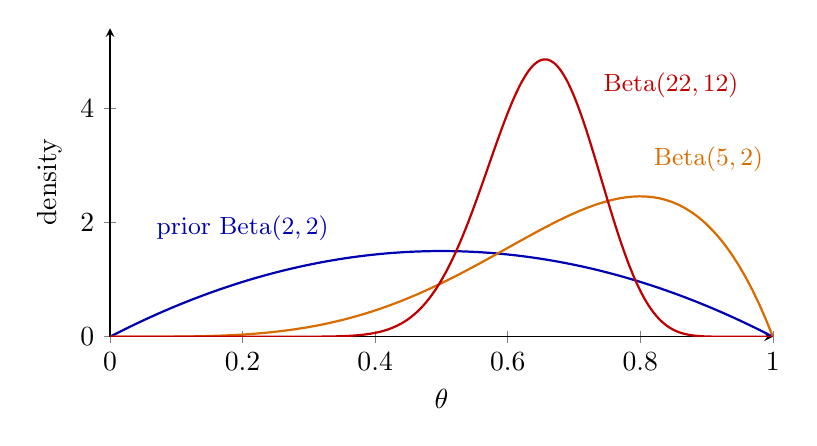
\begin{tikzpicture}
        \begin{axis}[width=10cm, height=5.5cm, xmin=0, xmax=1, ymin=0, ymax=5.4, axis lines=left, xlabel={$\theta$}, ylabel={density}, every axis plot/.append style={thick}]
            \addplot[blue!70!black, domain=0:1, samples=100] {6*x*(1-x)};
            \addplot[orange!85!black, domain=0:1, samples=100] {30*x^4*(1-x)};
            \addplot[red!75!black, smooth] coordinates {(0.00,0) (0.01,0.0000) (0.30,0.0009) (0.31,0.0015) (0.32,0.0025) (0.33,0.0040) (0.34,0.0064) (0.35,0.0099) (0.36,0.0151) (0.37,0.0226) (0.38,0.0332) (0.39,0.0479) (0.40,0.0679) (0.41,0.0948) (0.42,0.1304) (0.43,0.1765) (0.44,0.2354) (0.45,0.3095) (0.46,0.4013) (0.47,0.5132) (0.48,0.6476) (0.49,0.8064) (0.50,0.9913) (0.51,1.2031) (0.52,1.4418) (0.53,1.7063) (0.54,1.9943) (0.55,2.3022) (0.56,2.6249) (0.57,2.9560) (0.58,3.2879) (0.59,3.6116) (0.60,3.9176) (0.61,4.1959) (0.62,4.4364) (0.63,4.6297) (0.64,4.7675) (0.65,4.8430) (0.66,4.8515) (0.67,4.7908) (0.68,4.6615) (0.69,4.4668) (0.70,4.2129) (0.71,3.9083) (0.72,3.5637) (0.73,3.1913) (0.74,2.8039) (0.75,2.4144) (0.76,2.0351) (0.77,1.6769) (0.78,1.3484) (0.79,1.0563) (0.80,0.8043) (0.81,0.5938) (0.82,0.4239) (0.83,0.2916) (0.84,0.1925) (0.85,0.1213) (0.86,0.0726) (0.87,0.0410) (0.88,0.0216) (0.89,0.0105) (0.90,0.0047) (0.91,0.0018) (0.92,0.0006) (0.99,0.0000) (1.00,0)};
            \node[blue!70!black, font=\small] at (axis cs:0.2,1.9) {prior Beta$(2, 2)$};
            \node[orange!85!black, font=\small, left] at (axis cs:1.0,3.1) {Beta$(5, 2)$};
            \node[red!75!black, font=\small, right] at (axis cs:0.73,4.4) {Beta$(22, 12)$};
        \end{axis}
    \end{tikzpicture}
    \caption{Bayesian updating for the probability $\theta$ of heads: the prior Beta$(2, 2)$ (blue), the posterior Beta$(5, 2)$ after $3$ heads in $3$ flips (orange), and the posterior Beta$(22, 12)$ after $20$ heads in $30$ flips (red). With more data, the posterior concentrates around the relative frequency of heads.}
    \label{L4-fig:beta}
\end{figure}

To predict the next flip, Bayesian inference averages over all values of $\theta$, weighted by the posterior:
\[P(X_{N+1} = 1 \mid \mathcal{D}) = \int_0^1 \theta\,p(\theta \mid \mathcal{D}) \, d\theta = \E[\theta \mid \mathcal{D}] = \frac{a + k}{a + b + N}.\]
For the uniform prior ($a = b = 1$), this is Laplace's rule of succession $\frac{k + 1}{N + 2}$: after three heads in three flips, the probability of heads is $\frac{4}{5}$, not $1$. The same ``add pseudo-counts'' idea (Laplace smoothing) prevents zero probabilities for unseen words in language models.

\begin{example}[Credible intervals]\label{L4-ex:credible}
    A $95\%$ credible interval contains $\theta$ with posterior probability $0.95$, for example the interval between the $2.5\%$ and the $97.5\%$ quantiles of the posterior. For the posterior Beta$(22, 12)$ after $20$ heads in $30$ flips (Example~\ref{L4-ex:beta-coin}), it is $[0.48, 0.80]$ (computed numerically), close to the approximate confidence interval $\frac{2}{3} \pm 1.96\sqrt{\frac{2}{3} \cdot \frac{1}{3}/30} = [0.50, 0.84]$ of Section~\ref{L4-sec:estimation}. The interpretations differ: the credible interval makes a probability statement about $\theta$, given the data, while the confidence interval makes a probability statement about the random interval, for a fixed $\theta$. As the amount of data grows, the two intervals agree more and more (the Bernstein--von Mises theorem).
\end{example}

\begin{example}[Gamma--Poisson conjugacy]\label{L4-ex:gamma-poisson}
    Let the numbers of clicks on an ad in $N$ hours be i.i.d.\ Poisson$(\lambda)$, and let the prior of $\lambda$ be the Gamma distribution with the shape $a$ and the rate $b$, i.e., with the density $\frac{b^a}{\Gamma(a)}\lambda^{a-1}e^{-b\lambda}$ for $\lambda > 0$ and the mean $\frac{a}{b}$ (the Gamma distribution of Example~\ref{L4-ex:moments} with the scale $\frac{1}{b}$). If $S$ is the total number of clicks, the posterior is
    \[p(\lambda \mid \mathcal{D}) \propto e^{-N\lambda}\lambda^S \cdot \lambda^{a-1}e^{-b\lambda} = \lambda^{a + S - 1}e^{-(b + N)\lambda},\]
    i.e., Gamma$(a + S, b + N)$: the prior acts like $b$ previous hours with $a$ clicks in total. The posterior mean $\frac{a + S}{b + N}$ lies between the prior mean $\frac{a}{b}$ and the MLE $\frac{S}{N}$. For the prior Gamma$(2, 1)$ and the counts $3, 5, 4, 6, 2$ in five hours, the posterior is Gamma$(22, 6)$, with the mean $\frac{22}{6} \approx 3.67$ (the MLE is $4$) and the standard deviation $\frac{\sqrt{22}}{6} \approx 0.78$. The predictive probability of an hour without clicks is $\int e^{-\lambda}\,p(\lambda \mid \mathcal{D})\, d\lambda = \big(\frac{6}{7}\big)^{22} \approx 0.034$, while plugging in the MLE gives $e^{-4} \approx 0.018$: the posterior accounts for the uncertainty about $\lambda$.
\end{example}

\subsection{Maximum a posteriori estimation and regularization}

Often we only want a single parameter value. The maximum a posteriori (MAP) estimate is the mode of the posterior,
\[\hat\theta_{\text{MAP}} = \argmax_\theta p(\theta \mid \mathcal{D}) = \argmin_\theta \big(-\log p(\mathcal{D} \mid \theta) - \log p(\theta)\big),\]
since $p(\mathcal{D})$ does not depend on $\theta$. So MAP estimation minimizes the negative log-likelihood plus a penalty $-\log p(\theta)$ coming from the prior: a prior is a regularizer.

\begin{proposition}[Ridge regression as MAP estimation]\label{L4-prop:ridge-map}
    In the linear regression model of Proposition~\ref{L4-prop:ls-mle}, with the prior $\mathbf{w} \sim \mathcal{N}(\mathbf{0}, \alpha^{-1}I)$, the MAP estimate minimizes $\norm{\mathbf{y} - X\mathbf{w}}^2 + \lambda\norm{\mathbf{w}}^2$ with $\lambda = \alpha\sigma^2$, i.e., it is the ridge regression solution $\hat{\mathbf{w}} = (X^\top X + \lambda I)^{-1}X^\top\mathbf{y}$.
\end{proposition}

\begin{proof}
    Up to constants, $-\log p(\mathcal{D} \mid \mathbf{w}) - \log p(\mathbf{w}) = \frac{1}{2\sigma^2}\norm{\mathbf{y} - X\mathbf{w}}^2 + \frac{\alpha}{2}\norm{\mathbf{w}}^2$; multiply by $2\sigma^2$. The minimum was computed in the exercises of Lecture~3.
\end{proof}

A strong prior belief that the weights are small (large $\alpha$) means strong regularization. Similarly, the Laplace prior $p(\mathbf{w}) \propto e^{-\norm{\mathbf{w}}_1/b}$ leads to $\ell_1$ regularization (the lasso), which favors sparse weight vectors.

\subsection{Bayesian linear regression}

The MAP estimate discards the uncertainty that the posterior expresses. In linear regression with a Gaussian prior, the full posterior can be computed with the tools of Section~\ref{L4-sec:gaussian}.

\begin{theorem}[Posterior of Bayesian linear regression]\label{L4-thm:blr}
    In the model of Proposition~\ref{L4-prop:ls-mle} with the prior $\mathbf{w} \sim \mathcal{N}(\mathbf{0}, \alpha^{-1}I)$, the posterior is $\mathcal{N}(\mathbf{m}, S)$ with
    \[S = \big(\alpha I + \sigma^{-2}X^\top X\big)^{-1}, \qquad \mathbf{m} = \sigma^{-2}SX^\top\mathbf{y}.\]
    For a new input $\mathbf{x}_*$, the predictive distribution of $y_* = \mathbf{w}^\top\mathbf{x}_* + \varepsilon_*$ is $\mathcal{N}(\mathbf{m}^\top\mathbf{x}_*, \, \mathbf{x}_*^\top S\mathbf{x}_* + \sigma^2)$.
\end{theorem}

\begin{proof}
    Up to an additive constant that does not depend on $\mathbf{w}$,
    \[\log p(\mathbf{w} \mid \mathcal{D}) = -\frac{1}{2\sigma^2}\norm{\mathbf{y} - X\mathbf{w}}^2 - \frac{\alpha}{2}\norm{\mathbf{w}}^2 = -\frac{1}{2}\mathbf{w}^\top S^{-1}\mathbf{w} + \sigma^{-2}\mathbf{y}^\top X\mathbf{w} + \text{const}.\]
    Completing the square, this is $-\frac{1}{2}(\mathbf{w} - \mathbf{m})^\top S^{-1}(\mathbf{w} - \mathbf{m}) + \text{const}$, since the linear term of the latter is $\mathbf{m}^\top S^{-1}\mathbf{w} = \sigma^{-2}\mathbf{y}^\top X\mathbf{w}$. So the posterior density is proportional to the density of $\mathcal{N}(\mathbf{m}, S)$, hence equal to it. Given the data, $\mathbf{w}^\top\mathbf{x}_*$ is $\mathcal{N}(\mathbf{m}^\top\mathbf{x}_*, \mathbf{x}_*^\top S\mathbf{x}_*)$ by Corollary~\ref{L4-cor:gaussian-linear}, and adding the independent noise $\varepsilon_* \sim \mathcal{N}(0, \sigma^2)$ adds $\sigma^2$ to the variance.
\end{proof}

The posterior mean $\mathbf{m} = (X^\top X + \alpha\sigma^2 I)^{-1}X^\top\mathbf{y}$ is the ridge regression solution, which is also the MAP estimate (the mode and the mean of a Gaussian coincide). But the posterior also gives error bars: the predictive variance $\mathbf{x}_*^\top S\mathbf{x}_* + \sigma^2$ consists of the uncertainty about the weights, which shrinks as we collect more data, and the noise, which does not.

\begin{example}\label{L4-ex:blr}
    For the data $(1, 2), (2, 3), (3, 5)$, the model $y = wx + \varepsilon$ without intercept, $\alpha = 1$ and $\sigma^2 = 1$: $S = (1 + 1 + 4 + 9)^{-1} = \frac{1}{15}$ and $m = \frac{1}{15}(2 + 6 + 15) = \frac{23}{15} \approx 1.53$. At $x_* = 4$, the predictive distribution is $\mathcal{N}(6.13, \, \frac{16}{15} + 1) \approx \mathcal{N}(6.13, 2.07)$.
\end{example}

\subsection{Gaussian processes}\label{L4-sec:gp}

Bayesian linear regression puts a prior on the weights of a fixed set of features. A Gaussian process puts a prior directly on the unknown function.

\begin{definition}[Gaussian process]\label{L4-def:gp}
    A Gaussian process with mean function $m$ and covariance function (or kernel) $k$ is a random function $f$ such that for all points $\mathbf{x}_1, \ldots, \mathbf{x}_n$, the vector $(f(\mathbf{x}_1), \ldots, f(\mathbf{x}_n))$ is Gaussian with the mean vector $(m(\mathbf{x}_i))_i$ and the covariance matrix $K$ with entries $K_{ij} = k(\mathbf{x}_i, \mathbf{x}_j)$. We write $f \sim \mathcal{GP}(m, k)$.
\end{definition}

For this to make sense, every such matrix $K$ must be symmetric and positive semidefinite. This holds, for example, for $k(\mathbf{x}, \mathbf{x}') = \boldsymbol{\phi}(\mathbf{x})^\top\boldsymbol{\phi}(\mathbf{x}')$ with any feature map $\boldsymbol{\phi}$, since $K$ is then a Gram matrix (compare with the remark on kernels in Lecture~2).

\begin{example}\label{L4-ex:kernels}
    \begin{enumerate}
        \item (Linear kernel.) If $f(\mathbf{x}) = \mathbf{w}^\top\mathbf{x}$ with $\mathbf{w} \sim \mathcal{N}(\mathbf{0}, \alpha^{-1}I)$, then
        \[\Cov(f(\mathbf{x}), f(\mathbf{x}')) = \mathbf{x}^\top\Cov(\mathbf{w})\mathbf{x}' = \alpha^{-1}\mathbf{x}^\top\mathbf{x}'.\]
        So the prior of Bayesian linear regression is the Gaussian process with the kernel $k(\mathbf{x}, \mathbf{x}') = \alpha^{-1}\mathbf{x}^\top\mathbf{x}'$.
        \item (Squared exponential kernel.) $k(\mathbf{x}, \mathbf{x}') = \exp\big(-\frac{\norm{\mathbf{x} - \mathbf{x}'}^2}{2\ell^2}\big)$ gives smooth random functions, whose values at points closer than the length scale $\ell$ are strongly correlated. It corresponds to infinitely many features.
        \item (Brownian motion.) $k(s, t) = \min(s, t)$ for $s, t \geq 0$ is the covariance function of Brownian motion, a random function that we study in Section~\ref{L4-sec:sde}.
    \end{enumerate}
\end{example}

\begin{proposition}[Gaussian process regression]\label{L4-prop:gp-regression}
    Let $f \sim \mathcal{GP}(0, k)$, and let $y_i = f(\mathbf{x}_i) + \varepsilon_i$ for $i = 1, \ldots, N$, with i.i.d.\ noise $\varepsilon_i \sim \mathcal{N}(0, \sigma^2)$ independent of $f$. Let $K$ be the kernel matrix of the training inputs, and for a new input $\mathbf{x}_*$, let $\mathbf{k}_* = (k(\mathbf{x}_1, \mathbf{x}_*), \ldots, k(\mathbf{x}_N, \mathbf{x}_*))^\top$. Then, given the data,
    \[f(\mathbf{x}_*) \sim \mathcal{N}\big(\mathbf{k}_*^\top(K + \sigma^2 I)^{-1}\mathbf{y}, \ k(\mathbf{x}_*, \mathbf{x}_*) - \mathbf{k}_*^\top(K + \sigma^2 I)^{-1}\mathbf{k}_*\big).\]
\end{proposition}

\begin{proof}
    The vector $(\mathbf{y}, f(\mathbf{x}_*))$ is Gaussian with mean $\mathbf{0}$ and the covariance blocks $\Cov(\mathbf{y}) = K + \sigma^2 I$, $\Cov(\mathbf{y}, f(\mathbf{x}_*)) = \mathbf{k}_*$ and $\Var(f(\mathbf{x}_*)) = k(\mathbf{x}_*, \mathbf{x}_*)$; now apply Theorem~\ref{L4-thm:gaussian-conditional}.
\end{proof}

The posterior mean $\sum_i \alpha_i k(\mathbf{x}_i, \mathbf{x}_*)$ with $\boldsymbol{\alpha} = (K + \sigma^2 I)^{-1}\mathbf{y}$ is a combination of kernel functions centered at the data points; it is also the prediction of kernel ridge regression. The posterior variance does not depend on $\mathbf{y}$: it is small near the data, and it returns to the prior variance far away from them (Figure~\ref{L4-fig:gp}). For the linear kernel, the proposition reproduces the predictive distribution of Theorem~\ref{L4-thm:blr}.

\begin{example}\label{L4-ex:gp}
    With the squared exponential kernel ($\ell = 1$), $\sigma^2 = 0.1$, and the data $(0, 1)$ and $(1, 0)$: $K + \sigma^2 I = \begin{pmatrix} 1.1 & 0.607 \\ 0.607 & 1.1 \end{pmatrix}$, and at $x_* = 0.5$, $\mathbf{k}_* = (0.882, 0.882)^\top$. The posterior mean is $0.517$, and the posterior variance is $1 - \mathbf{k}_*^\top(K + \sigma^2 I)^{-1}\mathbf{k}_* \approx 0.087$; a new noisy observation at $x_*$ has the predictive variance $0.087 + 0.1 = 0.187$.
\end{example}

\begin{figure}[ht]
    \centering
    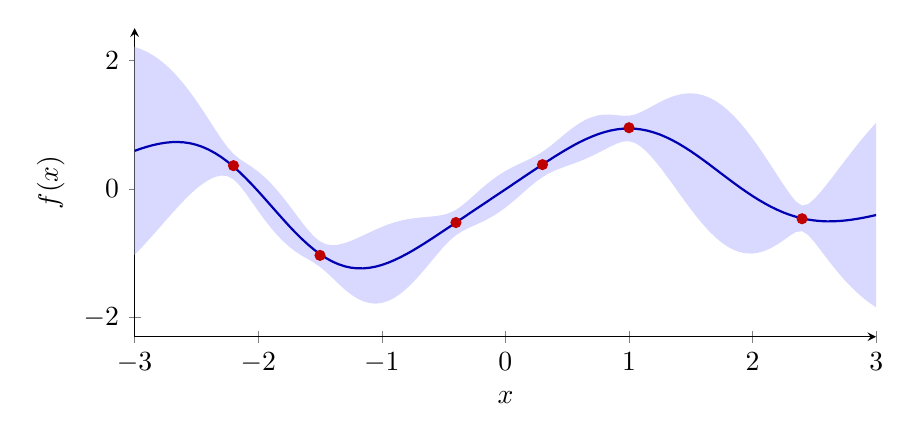
\begin{tikzpicture}
        \begin{axis}[width=11cm, height=5.5cm, xmin=-3, xmax=3, ymin=-2.3, ymax=2.5, axis lines=left, xlabel={$x$}, ylabel={$f(x)$}]
            \addplot[name path=upper, draw=none] coordinates {(-3.000,2.210) (-2.950,2.176) (-2.900,2.133) (-2.850,2.078) (-2.800,2.012) (-2.750,1.933) (-2.700,1.843) (-2.650,1.741) (-2.600,1.627) (-2.550,1.503) (-2.500,1.369) (-2.450,1.227) (-2.400,1.079) (-2.350,0.930) (-2.300,0.785) (-2.250,0.652) (-2.200,0.545) (-2.150,0.466) (-2.100,0.403) (-2.050,0.340) (-2.000,0.269) (-1.950,0.187) (-1.900,0.092) (-1.850,-0.014) (-1.800,-0.130) (-1.750,-0.253) (-1.700,-0.382) (-1.650,-0.510) (-1.600,-0.631) (-1.550,-0.737) (-1.500,-0.816) (-1.450,-0.862) (-1.400,-0.876) (-1.350,-0.867) (-1.300,-0.843) (-1.250,-0.808) (-1.200,-0.767) (-1.150,-0.722) (-1.100,-0.677) (-1.050,-0.633) (-1.000,-0.591) (-0.950,-0.554) (-0.900,-0.522) (-0.850,-0.495) (-0.800,-0.474) (-0.750,-0.459) (-0.700,-0.447) (-0.650,-0.438) (-0.600,-0.430) (-0.550,-0.419) (-0.500,-0.402) (-0.450,-0.372) (-0.400,-0.325) (-0.350,-0.258) (-0.300,-0.177) (-0.250,-0.091) (-0.200,-0.005) (-0.150,0.077) (-0.100,0.152) (-0.050,0.219) (0.000,0.279) (0.050,0.331) (0.100,0.379) (0.150,0.423) (0.200,0.469) (0.250,0.519) (0.300,0.578) (0.350,0.647) (0.400,0.724) (0.450,0.804) (0.500,0.884) (0.550,0.958) (0.600,1.024) (0.650,1.078) (0.700,1.118) (0.750,1.145) (0.800,1.157) (0.850,1.157) (0.900,1.148) (0.950,1.138) (1.000,1.139) (1.050,1.159) (1.100,1.198) (1.150,1.247) (1.200,1.300) (1.250,1.351) (1.300,1.398) (1.350,1.436) (1.400,1.465) (1.450,1.483) (1.500,1.488) (1.550,1.480) (1.600,1.457) (1.650,1.421) (1.700,1.369) (1.750,1.304) (1.800,1.224) (1.850,1.131) (1.900,1.026) (1.950,0.910) (2.000,0.784) (2.050,0.649) (2.100,0.507) (2.150,0.361) (2.200,0.212) (2.250,0.065) (2.300,-0.075) (2.350,-0.195) (2.400,-0.259) (2.450,-0.236) (2.500,-0.155) (2.550,-0.048) (2.600,0.071) (2.650,0.195) (2.700,0.321) (2.750,0.448) (2.800,0.572) (2.850,0.694) (2.900,0.812) (2.950,0.924) (3.000,1.031)};
            \addplot[name path=lower, draw=none] coordinates {(-3.000,-1.025) (-2.950,-0.925) (-2.900,-0.821) (-2.850,-0.714) (-2.800,-0.605) (-2.750,-0.495) (-2.700,-0.386) (-2.650,-0.280) (-2.600,-0.179) (-2.550,-0.083) (-2.500,0.004) (-2.450,0.079) (-2.400,0.141) (-2.350,0.186) (-2.300,0.208) (-2.250,0.199) (-2.200,0.148) (-2.150,0.053) (-2.100,-0.071) (-2.050,-0.207) (-2.000,-0.344) (-1.950,-0.476) (-1.900,-0.599) (-1.850,-0.711) (-1.800,-0.811) (-1.750,-0.898) (-1.700,-0.972) (-1.650,-1.035) (-1.600,-1.091) (-1.550,-1.147) (-1.500,-1.213) (-1.450,-1.293) (-1.400,-1.384) (-1.350,-1.477) (-1.300,-1.565) (-1.250,-1.641) (-1.200,-1.704) (-1.150,-1.749) (-1.100,-1.776) (-1.050,-1.785) (-1.000,-1.774) (-0.950,-1.744) (-0.900,-1.696) (-0.850,-1.631) (-0.800,-1.552) (-0.750,-1.458) (-0.700,-1.355) (-0.650,-1.243) (-0.600,-1.128) (-0.550,-1.012) (-0.500,-0.901) (-0.450,-0.802) (-0.400,-0.720) (-0.350,-0.658) (-0.300,-0.609) (-0.250,-0.566) (-0.200,-0.523) (-0.150,-0.476) (-0.100,-0.422) (-0.050,-0.360) (0.000,-0.291) (0.050,-0.214) (0.100,-0.132) (0.150,-0.047) (0.200,0.036) (0.250,0.115) (0.300,0.183) (0.350,0.240) (0.400,0.286) (0.450,0.324) (0.500,0.359) (0.550,0.393) (0.600,0.430) (0.650,0.469) (0.700,0.513) (0.750,0.560) (0.800,0.609) (0.850,0.659) (0.900,0.704) (0.950,0.736) (1.000,0.742) (1.050,0.714) (1.100,0.652) (1.150,0.565) (1.200,0.459) (1.250,0.340) (1.300,0.213) (1.350,0.081) (1.400,-0.054) (1.450,-0.187) (1.500,-0.316) (1.550,-0.440) (1.600,-0.556) (1.650,-0.661) (1.700,-0.755) (1.750,-0.835) (1.800,-0.901) (1.850,-0.951) (1.900,-0.985) (1.950,-1.004) (2.000,-1.005) (2.050,-0.991) (2.100,-0.962) (2.150,-0.919) (2.200,-0.863) (2.250,-0.799) (2.300,-0.730) (2.350,-0.671) (2.400,-0.657) (2.450,-0.718) (2.500,-0.828) (2.550,-0.953) (2.600,-1.080) (2.650,-1.203) (2.700,-1.320) (2.750,-1.430) (2.800,-1.530) (2.850,-1.622) (2.900,-1.705) (2.950,-1.778) (3.000,-1.842)};
            \addplot[blue!15] fill between[of=upper and lower];
            \addplot[blue!70!black, thick] coordinates {(-3.000,0.592) (-2.950,0.626) (-2.900,0.656) (-2.850,0.682) (-2.800,0.703) (-2.750,0.719) (-2.700,0.728) (-2.650,0.730) (-2.600,0.724) (-2.550,0.710) (-2.500,0.686) (-2.450,0.653) (-2.400,0.610) (-2.350,0.558) (-2.300,0.497) (-2.250,0.426) (-2.200,0.347) (-2.150,0.260) (-2.100,0.166) (-2.050,0.067) (-2.000,-0.037) (-1.950,-0.144) (-1.900,-0.253) (-1.850,-0.362) (-1.800,-0.470) (-1.750,-0.576) (-1.700,-0.677) (-1.650,-0.772) (-1.600,-0.861) (-1.550,-0.942) (-1.500,-1.015) (-1.450,-1.077) (-1.400,-1.130) (-1.350,-1.172) (-1.300,-1.204) (-1.250,-1.225) (-1.200,-1.235) (-1.150,-1.236) (-1.100,-1.227) (-1.050,-1.209) (-1.000,-1.183) (-0.950,-1.149) (-0.900,-1.109) (-0.850,-1.063) (-0.800,-1.013) (-0.750,-0.959) (-0.700,-0.901) (-0.650,-0.841) (-0.600,-0.779) (-0.550,-0.716) (-0.500,-0.652) (-0.450,-0.587) (-0.400,-0.522) (-0.350,-0.458) (-0.300,-0.393) (-0.250,-0.328) (-0.200,-0.264) (-0.150,-0.200) (-0.100,-0.135) (-0.050,-0.071) (0.000,-0.006) (0.050,0.058) (0.100,0.123) (0.150,0.188) (0.200,0.253) (0.250,0.317) (0.300,0.381) (0.350,0.443) (0.400,0.505) (0.450,0.564) (0.500,0.621) (0.550,0.676) (0.600,0.727) (0.650,0.773) (0.700,0.815) (0.750,0.852) (0.800,0.883) (0.850,0.908) (0.900,0.926) (0.950,0.937) (1.000,0.940) (1.050,0.937) (1.100,0.925) (1.150,0.906) (1.200,0.879) (1.250,0.846) (1.300,0.805) (1.350,0.758) (1.400,0.706) (1.450,0.648) (1.500,0.586) (1.550,0.520) (1.600,0.451) (1.650,0.380) (1.700,0.307) (1.750,0.234) (1.800,0.162) (1.850,0.090) (1.900,0.020) (1.950,-0.047) (2.000,-0.111) (2.050,-0.171) (2.100,-0.227) (2.150,-0.279) (2.200,-0.325) (2.250,-0.367) (2.300,-0.403) (2.350,-0.433) (2.400,-0.458) (2.450,-0.477) (2.500,-0.491) (2.550,-0.500) (2.600,-0.505) (2.650,-0.504) (2.700,-0.499) (2.750,-0.491) (2.800,-0.479) (2.850,-0.464) (2.900,-0.447) (2.950,-0.427) (3.000,-0.406)};
            \addplot[only marks, mark=*, mark size=1.8pt, red!75!black] coordinates {(-2.200,0.362) (-1.500,-1.034) (-0.400,-0.523) (0.300,0.378) (1.000,0.952) (2.400,-0.464)};
        \end{axis}
    \end{tikzpicture}
    \caption{Gaussian process regression with the squared exponential kernel ($\ell = 0.7$, $\sigma^2 = 0.01$) for six data points (red): the posterior mean (blue) and a band of $\pm 2$ posterior standard deviations. The uncertainty is small near the data and grows back to the prior standard deviation $1$ between and beyond them.}
    \label{L4-fig:gp}
\end{figure}

The hyperparameters, such as $\ell$ and $\sigma^2$, are usually chosen by maximizing the marginal likelihood $\log p(\mathbf{y}) = -\frac{1}{2}\mathbf{y}^\top(K + \sigma^2 I)^{-1}\mathbf{y} - \frac{1}{2}\log\det(K + \sigma^2 I) - \frac{N}{2}\log(2\pi)$, since $\mathbf{y} \sim \mathcal{N}(\mathbf{0}, K + \sigma^2 I)$; its gradient can be computed with the matrix calculus of Lecture~3. The cost of solving with the $N \times N$ matrix $K + \sigma^2 I$ grows like $N^3$, so exact Gaussian processes are limited to moderate data sets. Remarkably, one can show that neural networks with random weights become Gaussian processes in the limit of infinitely wide layers.

\begin{remark}[Beyond conjugate models]
    For most models, such as neural networks, the posterior has no closed form, and the evidence $p(\mathcal{D})$ is an intractable integral. Approximate methods include Markov chain Monte Carlo sampling (Section~\ref{L4-sec:markov}) and variational inference, which approximates the posterior by a simpler distribution by minimizing a Kullback--Leibler divergence (Section~\ref{L4-sec:information}).
\end{remark}

\section{Information Theory}\label{L4-sec:information}

Information theory measures uncertainty and the difference between distributions. Its quantities appear in machine learning as loss functions (cross-entropy), as regularizers (the KL term of variational autoencoders), and in the analysis of learning algorithms.

\begin{definition}[Entropy, cross-entropy and KL divergence]\label{L4-def:entropy}
    Let $p = (p_1, \ldots, p_K)$ and $q = (q_1, \ldots, q_K)$ be probability distributions on $\{1, \ldots, K\}$. The entropy of $p$, the cross-entropy of $q$ relative to $p$, and the Kullback--Leibler (KL) divergence of $q$ from $p$ are
    \[H(p) = -\sum_k p_k\log p_k, \qquad H(p, q) = -\sum_k p_k\log q_k, \qquad \KL(p \,\|\, q) = \sum_k p_k\log\frac{p_k}{q_k},\]
    with the conventions $0\log 0 = 0$ and $\KL(p \,\|\, q) = \infty$ if $q_k = 0 < p_k$ for some $k$.
\end{definition}

The number $-\log p_k$ measures the surprise of seeing the outcome $k$: rare outcomes are surprising. The entropy is the expected surprise. With $\log_2$ instead of $\log$, entropy is measured in bits, and it is the minimal average number of bits per symbol needed to encode outcomes of $p$ (Shannon's source coding theorem). A fair coin has entropy $1$ bit, a coin with $P(\text{heads}) = 0.9$ only $0.47$ bits, and a deterministic outcome $0$ bits. Clearly $H(p) \geq 0$, and
\[H(p, q) = H(p) + \KL(p \,\|\, q):\]
the cross-entropy is the average number of bits if we encode outcomes of $p$ with a code designed for $q$, and the KL divergence is the number of extra bits we pay for using the wrong distribution.

\begin{theorem}[Gibbs' inequality]\label{L4-thm:gibbs}
    $\KL(p \,\|\, q) \geq 0$, with equality if and only if $p = q$.
\end{theorem}

\begin{proof}
    We may assume $q_k > 0$ whenever $p_k > 0$. Let $T$ be the set of $k$ with $p_k > 0$, and let $R$ be the random variable that takes the value $\frac{q_k}{p_k}$ with probability $p_k$, for $k \in T$. By Jensen's inequality for the concave function $\log$ (Theorem~\ref{L4-thm:jensen}),
    \[-\KL(p \,\|\, q) = \sum_{k \in T} p_k\log\frac{q_k}{p_k} = \E[\log R] \leq \log\E[R] = \log\sum_{k \in T} q_k \leq \log 1 = 0.\]
    If equality holds, then $\sum_{k \in T} q_k = 1$, and equality holds in Jensen's inequality, which for the strictly concave $\log$ happens only if $R$ is constant; so $q_k = c\,p_k$ for $k \in T$ and $q_k = 0$ otherwise, and $c = 1$ since both sum to $1$.
\end{proof}

Two consequences: the cross-entropy $H(p, q)$ is minimal for $q = p$, and for the uniform distribution $u$ on $K$ outcomes, $0 \leq \KL(p \,\|\, u) = \log K - H(p)$, so $H(p) \leq \log K$: the uniform distribution has maximal entropy (compare with the exercise on maximum entropy in Lecture~3). The KL divergence is not a distance in the sense of Lecture~2, since it is not symmetric. For $p = (\frac{1}{2}, \frac{1}{2})$ and $q = (0.9, 0.1)$, $\KL(p \,\|\, q) \approx 0.511$ but $\KL(q \,\|\, p) \approx 0.368$.

\begin{theorem}[Maximum likelihood minimizes the KL divergence]\label{L4-thm:mle-kl}
    Let $x_1, \ldots, x_N \in \{1, \ldots, K\}$ be data with the empirical distribution $\hat p$, i.e., $\hat p_k$ is the fraction of data points equal to $k$, and let $q_\theta$ be a model distribution. Then
    \[\frac{1}{N}\sum_{i=1}^N \log q_\theta(x_i) = -H(\hat p, q_\theta) = -H(\hat p) - \KL(\hat p \,\|\, q_\theta).\]
    So maximizing the likelihood is the same as minimizing the cross-entropy $H(\hat p, q_\theta)$, and the same as minimizing $\KL(\hat p \,\|\, q_\theta)$.
\end{theorem}

\begin{proof}
    Grouping the data points by their values, $\frac{1}{N}\sum_i \log q_\theta(x_i) = \sum_k \hat p_k\log q_\theta(k) = -H(\hat p, q_\theta)$. The term $H(\hat p)$ does not depend on $\theta$.
\end{proof}

This is why the loss of classifiers is called the cross-entropy loss: for each training example, it is the cross-entropy between the one-hot distribution of the true label and the predicted distribution, and training fits the model distribution to the data in the sense of the KL divergence.

\paragraph{Continuous distributions.} For densities, the sums become integrals: the differential entropy is $h(p) = -\int p(x)\log p(x)\, dx$, and $\KL(p \,\|\, q) = \int p(x)\log\frac{p(x)}{q(x)}\, dx \geq 0$. The differential entropy of $\mathcal{N}(\mu, \sigma^2)$ is $\frac{1}{2}\log(2\pi e\sigma^2)$, and among all densities with variance $\sigma^2$, the Gaussian has the largest entropy.

\begin{example}[Maximum entropy]\label{L4-ex:max-entropy}
    Among the distributions on $\mathbb{R}$ with the variance $1$, the uniform distribution on $[-\sqrt{3}, \sqrt{3}]$ has the differential entropy $\log(2\sqrt{3}) \approx 1.24$, the Laplace distribution with the density $\frac{1}{\sqrt{2}}e^{-\sqrt{2}|x|}$ has $1 + \frac{1}{2}\log 2 \approx 1.35$, and $\mathcal{N}(0, 1)$ has the largest value, $\frac{1}{2}\log(2\pi e) \approx 1.42$ nats. In fact, for every density $p$ with mean $0$ and variance $1$, $\KL(p \,\|\, \mathcal{N}(0, 1)) = -h(p) + \E_p\big[\frac{1}{2}\log(2\pi) + \frac{X^2}{2}\big] = \frac{1}{2}\log(2\pi e) - h(p)$, which is nonnegative by Gibbs' inequality. This proves the maximum entropy property of the Gaussian, which is one justification for Gaussian noise models: they assume nothing beyond the variance.
\end{example}

\begin{proposition}[KL divergence between Gaussians]\label{L4-prop:kl-gaussian}
    For $p = \mathcal{N}(\mu_1, \sigma_1^2)$ and $q = \mathcal{N}(\mu_2, \sigma_2^2)$,
    \[\KL(p \,\|\, q) = \log\frac{\sigma_2}{\sigma_1} + \frac{\sigma_1^2 + (\mu_1 - \mu_2)^2}{2\sigma_2^2} - \frac{1}{2}.\]
\end{proposition}

\begin{proof}
    $\log\frac{p(x)}{q(x)} = \log\frac{\sigma_2}{\sigma_1} - \frac{(x - \mu_1)^2}{2\sigma_1^2} + \frac{(x - \mu_2)^2}{2\sigma_2^2}$. Take the expectation for $X \sim p$, using $\E[(X - \mu_1)^2] = \sigma_1^2$ and $\E[(X - \mu_2)^2] = \sigma_1^2 + (\mu_1 - \mu_2)^2$.
\end{proof}

In a variational autoencoder, each data point is encoded as a Gaussian $\mathcal{N}(\mu, \sigma^2)$ (in each latent dimension), and the loss contains the term $\KL\big(\mathcal{N}(\mu, \sigma^2) \,\|\, \mathcal{N}(0, 1)\big) = \frac{1}{2}(\mu^2 + \sigma^2 - 1 - \log\sigma^2)$, which keeps the codes close to a standard Gaussian. For example, for $\mu = 1$ and $\sigma = 2$, it is $\frac{1}{2}(4 - \log 4) \approx 1.31$.

\paragraph{Mutual information.} The mutual information of two random variables is the KL divergence between their joint distribution and the product of their marginals,
\[I(X; Y) = \KL\big(p(x, y) \,\|\, p_X(x)p_Y(y)\big) = \sum_{x, y} p(x, y)\log\frac{p(x, y)}{p_X(x)p_Y(y)}.\]
By Gibbs' inequality, $I(X; Y) \geq 0$, with equality if and only if $X$ and $Y$ are independent. Unlike the correlation, it detects every kind of dependence. For Example~\ref{L4-ex:joint-table}, $I(X; Y) \approx 0.086$ nats.

\section{Stochastic Differential Equations}\label{L4-sec:sde}

Markov chains (Section~\ref{L4-sec:markov}) move in discrete steps. Many random processes change continuously in time: the position of a particle in a fluid, the price of a stock, the parameters of a network during training with stochastic gradients, or the gradually noised images of a diffusion model. Stochastic differential equations (SDEs) describe such processes by adding random noise to ordinary differential equations (Section~\ref{L3-sec:ode}). The source of the noise is Brownian motion.

\begin{definition}[Brownian motion]\label{L4-def:brownian}
    A Brownian motion (or Wiener process) is a family of random variables $B(t)$, $t \geq 0$, with $B(0) = 0$, such that
    \begin{enumerate}
        \item for $0 \leq t_0 < t_1 < \cdots < t_k$, the increments $B(t_1) - B(t_0), \ldots, B(t_k) - B(t_{k-1})$ are independent;
        \item $B(t) - B(s) \sim \mathcal{N}(0, t - s)$ for $s < t$;
        \item the paths $t \mapsto B(t)$ are continuous.
    \end{enumerate}
\end{definition}

That such a process exists is a theorem of Norbert Wiener, which we do not prove. On the grid $t_k = kh$, Brownian motion is simulated exactly by the random walk $B(t_{k+1}) = B(t_k) + \sqrt{h}\,Z_k$ with i.i.d.\ $Z_k \sim \mathcal{N}(0, 1)$ (Figure~\ref{L4-fig:sde}). Conversely, by the central limit theorem, every random walk with many small independent steps looks like a Brownian motion from far away.

\begin{proposition}\label{L4-prop:brownian}
    $\E[B(t)] = 0$, $\Var(B(t)) = t$, and $\Cov(B(s), B(t)) = \min(s, t)$.
\end{proposition}

\begin{proof}
    The first two statements are property (2) with $s = 0$. For $s \leq t$, $\Cov(B(s), B(t)) = \Cov\big(B(s), B(s) + (B(t) - B(s))\big) = \Var(B(s)) + 0 = s$, since the increment $B(t) - B(s)$ is independent of $B(s) = B(s) - B(0)$.
\end{proof}

So Brownian motion is a Gaussian process with mean $0$ and covariance function $\min(s, t)$ (Section~\ref{L4-sec:gp}). Its typical displacement in a time $h$ is $\sqrt{h}$, which is much larger than $h$ for small $h$: the difference quotient $\frac{B(t + h) - B(t)}{h}$ has the variance $\frac{1}{h} \to \infty$. In fact, the paths of Brownian motion are continuous but nowhere differentiable, and ordinary calculus does not apply to them.

With the filtration $\mathcal{F}_s = \sigma(B(u) : u \leq s)$, the independence of the increments gives $\E[B(t) \mid \mathcal{F}_s] = B(s) + \E[B(t) - B(s)] = B(s)$ for $s \leq t$: Brownian motion is a martingale in continuous time (Section~\ref{L4-sec:martingales}), the continuous analogue of a fair random walk.

\begin{definition}[Stochastic differential equation]\label{L4-def:sde}
    An SDE $dX = \mu(X)\,dt + \sigma(X)\,dB$, with drift $\mu$ and diffusion coefficient $\sigma$, describes a process with $X(t) = X(0) + \int_0^t \mu(X(s))\, ds + \int_0^t \sigma(X(s))\, dB(s)$, where the last integral is a stochastic (It\^o) integral. Its Euler--Maruyama approximation with step $h$ is
    \[X_{k+1} = X_k + \mu(X_k)\,h + \sigma(X_k)\sqrt{h}\,Z_k, \qquad Z_k \sim \mathcal{N}(0, 1) \text{ i.i.d.}\]
\end{definition}

We do not define the stochastic integral; for our purposes, the Euler--Maruyama scheme, which converges to the solution as $h \to 0$, can serve as the definition. It is Euler's method for the ODE $x' = \mu(x)$ (Section~\ref{L3-sec:euler}), plus Gaussian noise whose standard deviation is proportional to $\sqrt{h}$, and it is a Markov chain with continuous states. For $\sigma = 0$, the SDE is an ODE.

\begin{example}[The Ornstein--Uhlenbeck process]\label{L4-ex:ou}
    The SDE $dX = -\theta X\,dt + \sigma\,dB$ with $\theta > 0$ pulls $X$ towards $0$ while the noise pushes it around. Its Euler--Maruyama approximation is $X_{k+1} = (1 - \theta h)X_k + \sigma\sqrt{h}\,Z_k$. Its mean satisfies $\E[X_{k+1}] = (1 - \theta h)\E[X_k]$, so it follows Euler's method for the ODE $x' = -\theta x$, with the solution $e^{-\theta t}X(0)$. If $X_k \sim \mathcal{N}(0, v)$ is independent of $Z_k$, then $X_{k+1} \sim \mathcal{N}\big(0, (1 - \theta h)^2v + \sigma^2h\big)$ by Corollary~\ref{L4-cor:gaussian-linear}. So for $0 < \theta h < 2$, the chain has the stationary distribution $\mathcal{N}(0, v_h)$ with
    \[v_h = \frac{\sigma^2h}{1 - (1 - \theta h)^2} = \frac{\sigma^2}{\theta(2 - \theta h)} \to \frac{\sigma^2}{2\theta} \qquad \text{as } h \to 0.\]
    For $\theta = 1$, $\sigma = \sqrt{2}$, the stationary distribution of the SDE is $\mathcal{N}(0, 1)$ (Figure~\ref{L4-fig:sde}); for $\theta = \sigma = 1$ and $h = 0.01$, $v_h \approx 0.5025$ instead of $0.5$.
\end{example}

\begin{figure}[ht]
    \centering
    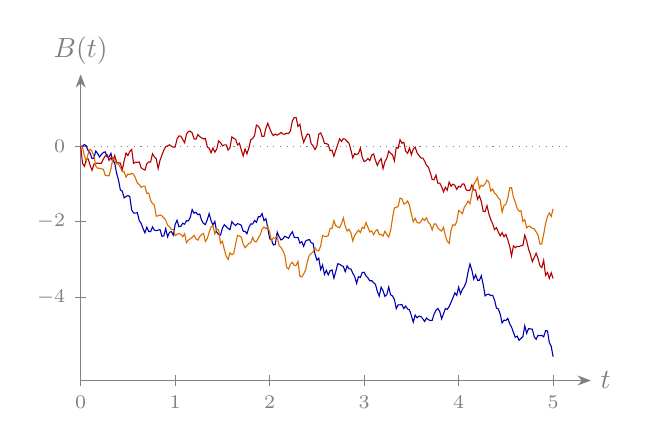
\begin{tikzpicture}[x=1.2cm, y=0.48cm, >=Stealth]
        \draw[->, gray] (0,-6.2) -- (5.4,-6.2) node[right] {$t$};
        \draw[->, gray] (0,-6.2) -- (0,1.9) node[above] {$B(t)$};
        \draw[gray, dotted] (0,0) -- (5.2,0);
        \foreach \v in {-4,-2,0}
            \draw[gray] (0.06,\v) -- (-0.06,\v) node[left, font=\scriptsize] {$\v$};
        \foreach \v in {0,...,5}
            \draw[gray] (\v,-6.05) -- (\v,-6.35) node[below, font=\scriptsize] {$\v$};
        \draw[blue!70!black] plot coordinates {(0.00,0.000) (0.02,0.000) (0.04,0.042) (0.06,0.004) (0.08,-0.122) (0.10,-0.187) (0.12,-0.327) (0.14,-0.318) (0.16,-0.129) (0.18,-0.198) (0.20,-0.286) (0.22,-0.217) (0.24,-0.166) (0.26,-0.151) (0.28,-0.283) (0.30,-0.287) (0.32,-0.189) (0.34,-0.379) (0.36,-0.444) (0.38,-0.713) (0.40,-0.895) (0.42,-1.155) (0.44,-1.189) (0.46,-1.368) (0.48,-1.330) (0.50,-1.307) (0.52,-1.334) (0.54,-1.690) (0.56,-1.766) (0.58,-1.773) (0.60,-1.757) (0.62,-1.973) (0.64,-2.041) (0.66,-2.179) (0.68,-2.293) (0.70,-2.143) (0.72,-2.258) (0.74,-2.262) (0.76,-2.137) (0.78,-2.220) (0.80,-2.236) (0.82,-2.220) (0.84,-2.211) (0.86,-2.384) (0.88,-2.373) (0.90,-2.181) (0.92,-2.400) (0.94,-2.278) (0.96,-2.262) (0.98,-2.352) (1.00,-2.069) (1.02,-1.962) (1.04,-2.131) (1.06,-2.121) (1.08,-2.039) (1.10,-2.066) (1.12,-1.969) (1.14,-1.979) (1.16,-1.884) (1.18,-1.681) (1.20,-1.776) (1.22,-1.748) (1.24,-1.813) (1.26,-1.795) (1.28,-1.963) (1.30,-2.045) (1.32,-2.073) (1.34,-1.946) (1.36,-1.784) (1.38,-1.971) (1.40,-2.083) (1.42,-1.992) (1.44,-2.274) (1.46,-2.339) (1.48,-2.353) (1.50,-2.175) (1.52,-2.078) (1.54,-2.124) (1.56,-2.176) (1.58,-2.211) (1.60,-1.996) (1.62,-2.056) (1.64,-2.099) (1.66,-2.049) (1.68,-2.067) (1.70,-2.094) (1.72,-2.252) (1.74,-2.254) (1.76,-2.316) (1.78,-2.151) (1.80,-2.059) (1.82,-2.062) (1.84,-1.968) (1.86,-2.016) (1.88,-1.867) (1.90,-1.868) (1.92,-1.785) (1.94,-1.968) (1.96,-1.919) (1.98,-2.158) (2.00,-2.446) (2.02,-2.489) (2.04,-2.616) (2.06,-2.593) (2.08,-2.275) (2.10,-2.393) (2.12,-2.481) (2.14,-2.452) (2.16,-2.382) (2.18,-2.407) (2.20,-2.436) (2.22,-2.337) (2.24,-2.264) (2.26,-2.410) (2.28,-2.421) (2.30,-2.416) (2.32,-2.565) (2.34,-2.528) (2.36,-2.650) (2.38,-2.512) (2.40,-2.485) (2.42,-2.472) (2.44,-2.556) (2.46,-2.573) (2.48,-2.855) (2.50,-3.015) (2.52,-2.964) (2.54,-3.265) (2.56,-3.145) (2.58,-3.392) (2.60,-3.285) (2.62,-3.405) (2.64,-3.295) (2.66,-3.276) (2.68,-3.493) (2.70,-3.317) (2.72,-3.113) (2.74,-3.122) (2.76,-3.161) (2.78,-3.183) (2.80,-3.321) (2.82,-3.166) (2.84,-3.243) (2.86,-3.250) (2.88,-3.362) (2.90,-3.451) (2.92,-3.631) (2.94,-3.454) (2.96,-3.475) (2.98,-3.339) (3.00,-3.337) (3.02,-3.435) (3.04,-3.481) (3.06,-3.561) (3.08,-3.559) (3.10,-3.613) (3.12,-3.655) (3.14,-3.850) (3.16,-3.964) (3.18,-3.730) (3.20,-3.825) (3.22,-3.974) (3.24,-3.926) (3.26,-3.727) (3.28,-3.933) (3.30,-3.962) (3.32,-4.052) (3.34,-4.301) (3.36,-4.197) (3.38,-4.200) (3.40,-4.190) (3.42,-4.297) (3.44,-4.232) (3.46,-4.309) (3.48,-4.329) (3.50,-4.485) (3.52,-4.657) (3.54,-4.469) (3.56,-4.540) (3.58,-4.499) (3.60,-4.504) (3.62,-4.566) (3.64,-4.638) (3.66,-4.549) (3.68,-4.592) (3.70,-4.613) (3.72,-4.610) (3.74,-4.444) (3.76,-4.347) (3.78,-4.293) (3.80,-4.373) (3.82,-4.568) (3.84,-4.434) (3.86,-4.297) (3.88,-4.317) (3.90,-4.241) (3.92,-4.130) (3.94,-4.013) (3.96,-3.882) (3.98,-3.947) (4.00,-3.732) (4.02,-3.909) (4.04,-3.787) (4.06,-3.717) (4.08,-3.593) (4.10,-3.328) (4.12,-3.118) (4.14,-3.280) (4.16,-3.519) (4.18,-3.403) (4.20,-3.547) (4.22,-3.548) (4.24,-3.430) (4.26,-3.662) (4.28,-3.960) (4.30,-3.924) (4.32,-3.918) (4.34,-3.952) (4.36,-3.947) (4.38,-4.069) (4.40,-4.283) (4.42,-4.306) (4.44,-4.444) (4.46,-4.676) (4.48,-4.604) (4.50,-4.613) (4.52,-4.556) (4.54,-4.696) (4.56,-4.789) (4.58,-4.930) (4.60,-5.055) (4.62,-5.028) (4.64,-5.138) (4.66,-5.088) (4.68,-5.040) (4.70,-4.754) (4.72,-4.951) (4.74,-4.825) (4.76,-4.838) (4.78,-4.840) (4.80,-5.045) (4.82,-5.110) (4.84,-5.005) (4.86,-5.016) (4.88,-5.005) (4.90,-5.046) (4.92,-4.883) (4.94,-4.886) (4.96,-5.197) (4.98,-5.295) (5.00,-5.573)};
        \draw[red!70!black] plot coordinates {(0.00,0.000) (0.02,-0.460) (0.04,-0.535) (0.06,-0.346) (0.08,-0.340) (0.10,-0.505) (0.12,-0.638) (0.14,-0.479) (0.16,-0.456) (0.18,-0.449) (0.20,-0.457) (0.22,-0.452) (0.24,-0.338) (0.26,-0.260) (0.28,-0.229) (0.30,-0.376) (0.32,-0.304) (0.34,-0.401) (0.36,-0.246) (0.38,-0.426) (0.40,-0.445) (0.42,-0.447) (0.44,-0.634) (0.46,-0.390) (0.48,-0.184) (0.50,-0.249) (0.52,-0.140) (0.54,-0.087) (0.56,-0.456) (0.58,-0.421) (0.60,-0.430) (0.62,-0.418) (0.64,-0.570) (0.66,-0.608) (0.68,-0.633) (0.70,-0.465) (0.72,-0.418) (0.74,-0.419) (0.76,-0.203) (0.78,-0.281) (0.80,-0.336) (0.82,-0.593) (0.84,-0.371) (0.86,-0.235) (0.88,-0.105) (0.90,-0.011) (0.92,0.005) (0.94,0.035) (0.96,-0.000) (0.98,-0.029) (1.00,-0.021) (1.02,0.192) (1.04,0.271) (1.06,0.263) (1.08,0.181) (1.10,0.091) (1.12,0.318) (1.14,0.389) (1.16,0.399) (1.18,0.350) (1.20,0.193) (1.22,0.184) (1.24,0.307) (1.26,0.252) (1.28,0.220) (1.30,0.188) (1.32,0.204) (1.34,-0.021) (1.36,-0.055) (1.38,-0.176) (1.40,-0.050) (1.42,-0.159) (1.44,-0.078) (1.46,0.138) (1.48,0.093) (1.50,0.008) (1.52,0.035) (1.54,0.035) (1.56,-0.105) (1.58,-0.040) (1.60,0.245) (1.62,0.208) (1.64,0.180) (1.66,0.032) (1.68,0.077) (1.70,-0.099) (1.72,-0.256) (1.74,-0.075) (1.76,-0.203) (1.78,-0.050) (1.80,0.165) (1.82,0.202) (1.84,0.280) (1.86,0.557) (1.88,0.529) (1.90,0.445) (1.92,0.253) (1.94,0.259) (1.96,0.469) (1.98,0.604) (2.00,0.471) (2.02,0.350) (2.04,0.279) (2.06,0.320) (2.08,0.291) (2.10,0.321) (2.12,0.363) (2.14,0.321) (2.16,0.315) (2.18,0.345) (2.20,0.333) (2.22,0.404) (2.24,0.669) (2.26,0.752) (2.28,0.760) (2.30,0.522) (2.32,0.577) (2.34,0.301) (2.36,0.102) (2.38,0.223) (2.40,0.323) (2.42,0.302) (2.44,0.060) (2.46,0.007) (2.48,-0.089) (2.50,0.001) (2.52,0.321) (2.54,0.351) (2.56,0.241) (2.58,0.075) (2.60,0.068) (2.62,0.043) (2.64,-0.120) (2.66,-0.104) (2.68,-0.267) (2.70,-0.109) (2.72,0.041) (2.74,0.194) (2.76,0.127) (2.78,0.200) (2.80,0.181) (2.82,0.126) (2.84,0.078) (2.86,-0.105) (2.88,-0.310) (2.90,-0.197) (2.92,-0.224) (2.94,-0.194) (2.96,-0.052) (2.98,-0.297) (3.00,-0.408) (3.02,-0.383) (3.04,-0.328) (3.06,-0.381) (3.08,-0.236) (3.10,-0.206) (3.12,-0.377) (3.14,-0.509) (3.16,-0.395) (3.18,-0.330) (3.20,-0.598) (3.22,-0.407) (3.24,-0.323) (3.26,-0.133) (3.28,-0.187) (3.30,-0.229) (3.32,-0.388) (3.34,-0.030) (3.36,-0.054) (3.38,0.170) (3.40,0.079) (3.42,0.102) (3.44,-0.135) (3.46,-0.189) (3.48,-0.050) (3.50,-0.227) (3.52,-0.075) (3.54,-0.027) (3.56,-0.175) (3.58,-0.246) (3.60,-0.311) (3.62,-0.318) (3.64,-0.394) (3.66,-0.511) (3.68,-0.554) (3.70,-0.699) (3.72,-0.881) (3.74,-0.888) (3.76,-0.763) (3.78,-0.980) (3.80,-0.979) (3.82,-1.071) (3.84,-1.209) (3.86,-1.088) (3.88,-1.162) (3.90,-0.950) (3.92,-1.060) (3.94,-1.005) (3.96,-1.038) (3.98,-1.144) (4.00,-1.061) (4.02,-1.083) (4.04,-0.998) (4.06,-1.004) (4.08,-1.158) (4.10,-1.172) (4.12,-1.165) (4.14,-1.030) (4.16,-1.158) (4.18,-1.163) (4.20,-1.407) (4.22,-1.315) (4.24,-1.468) (4.26,-1.723) (4.28,-1.731) (4.30,-1.575) (4.32,-1.791) (4.34,-1.944) (4.36,-2.050) (4.38,-2.209) (4.40,-2.156) (4.42,-2.270) (4.44,-2.372) (4.46,-2.289) (4.48,-2.396) (4.50,-2.335) (4.52,-2.472) (4.54,-2.644) (4.56,-2.903) (4.58,-2.640) (4.60,-2.685) (4.62,-2.651) (4.64,-2.655) (4.66,-2.633) (4.68,-2.626) (4.70,-2.356) (4.72,-2.503) (4.74,-2.723) (4.76,-2.866) (4.78,-3.055) (4.80,-2.949) (4.82,-2.833) (4.84,-2.969) (4.86,-3.166) (4.88,-3.216) (4.90,-3.019) (4.92,-3.418) (4.94,-3.344) (4.96,-3.496) (4.98,-3.349) (5.00,-3.501)};
        \draw[orange!85!black] plot coordinates {(0.00,0.000) (0.02,-0.040) (0.04,-0.253) (0.06,-0.392) (0.08,-0.196) (0.10,-0.080) (0.12,-0.136) (0.14,-0.259) (0.16,-0.527) (0.18,-0.583) (0.20,-0.587) (0.22,-0.599) (0.24,-0.612) (0.26,-0.771) (0.28,-0.780) (0.30,-0.786) (0.32,-0.603) (0.34,-0.339) (0.36,-0.359) (0.38,-0.467) (0.40,-0.476) (0.42,-0.562) (0.44,-0.667) (0.46,-0.676) (0.48,-0.823) (0.50,-0.737) (0.52,-0.752) (0.54,-0.717) (0.56,-0.743) (0.58,-0.845) (0.60,-0.980) (0.62,-1.013) (0.64,-1.091) (0.66,-1.058) (0.68,-1.058) (0.70,-1.251) (0.72,-1.241) (0.74,-1.431) (0.76,-1.518) (0.78,-1.560) (0.80,-1.854) (0.82,-1.841) (0.84,-1.819) (0.86,-1.842) (0.88,-1.902) (0.90,-1.955) (0.92,-2.093) (0.94,-2.131) (0.96,-2.209) (0.98,-2.196) (1.00,-2.366) (1.02,-2.333) (1.04,-2.313) (1.06,-2.333) (1.08,-2.395) (1.10,-2.317) (1.12,-2.552) (1.14,-2.487) (1.16,-2.453) (1.18,-2.413) (1.20,-2.358) (1.22,-2.451) (1.24,-2.487) (1.26,-2.397) (1.28,-2.336) (1.30,-2.307) (1.32,-2.521) (1.34,-2.445) (1.36,-2.280) (1.38,-2.137) (1.40,-2.104) (1.42,-2.324) (1.44,-2.191) (1.46,-2.212) (1.48,-2.570) (1.50,-2.517) (1.52,-2.728) (1.54,-2.911) (1.56,-3.001) (1.58,-2.821) (1.60,-2.873) (1.62,-2.835) (1.64,-2.588) (1.66,-2.362) (1.68,-2.377) (1.70,-2.411) (1.72,-2.589) (1.74,-2.688) (1.76,-2.628) (1.78,-2.572) (1.80,-2.556) (1.82,-2.415) (1.84,-2.524) (1.86,-2.532) (1.88,-2.429) (1.90,-2.346) (1.92,-2.195) (1.94,-2.139) (1.96,-2.183) (1.98,-2.131) (2.00,-2.273) (2.02,-2.505) (2.04,-2.423) (2.06,-2.431) (2.08,-2.387) (2.10,-2.627) (2.12,-2.679) (2.14,-2.764) (2.16,-2.886) (2.18,-3.205) (2.20,-3.252) (2.22,-3.125) (2.24,-3.071) (2.26,-3.156) (2.28,-3.158) (2.30,-3.051) (2.32,-3.442) (2.34,-3.459) (2.36,-3.383) (2.38,-3.286) (2.40,-3.046) (2.42,-2.885) (2.44,-2.841) (2.46,-2.798) (2.48,-2.687) (2.50,-2.763) (2.52,-2.769) (2.54,-2.641) (2.56,-2.364) (2.58,-2.386) (2.60,-2.393) (2.62,-2.365) (2.64,-2.175) (2.66,-2.179) (2.68,-1.972) (2.70,-2.108) (2.72,-2.135) (2.74,-2.163) (2.76,-2.051) (2.78,-1.904) (2.80,-2.117) (2.82,-2.247) (2.84,-2.199) (2.86,-2.292) (2.88,-2.507) (2.90,-2.360) (2.92,-2.291) (2.94,-2.221) (2.96,-2.288) (2.98,-2.143) (3.00,-2.177) (3.02,-2.021) (3.04,-2.150) (3.06,-2.271) (3.08,-2.242) (3.10,-2.342) (3.12,-2.246) (3.14,-2.209) (3.16,-2.340) (3.18,-2.329) (3.20,-2.379) (3.22,-2.250) (3.24,-2.339) (3.26,-2.401) (3.28,-2.230) (3.30,-1.913) (3.32,-1.631) (3.34,-1.622) (3.36,-1.591) (3.38,-1.374) (3.40,-1.391) (3.42,-1.530) (3.44,-1.513) (3.46,-1.449) (3.48,-1.566) (3.50,-1.799) (3.52,-2.002) (3.54,-1.908) (3.56,-2.016) (3.58,-2.036) (3.60,-2.005) (3.62,-1.918) (3.64,-1.965) (3.66,-1.895) (3.68,-2.021) (3.70,-2.072) (3.72,-2.217) (3.74,-2.057) (3.76,-2.060) (3.78,-2.165) (3.80,-2.215) (3.82,-2.246) (3.84,-2.147) (3.86,-2.373) (3.88,-2.519) (3.90,-2.573) (3.92,-2.215) (3.94,-2.080) (3.96,-2.095) (3.98,-1.995) (4.00,-1.704) (4.02,-1.737) (4.04,-1.789) (4.06,-1.617) (4.08,-1.547) (4.10,-1.452) (4.12,-1.524) (4.14,-1.252) (4.16,-1.010) (4.18,-0.930) (4.20,-0.834) (4.22,-1.120) (4.24,-1.030) (4.26,-1.058) (4.28,-0.996) (4.30,-0.900) (4.32,-0.948) (4.34,-1.187) (4.36,-1.135) (4.38,-1.240) (4.40,-1.287) (4.42,-1.372) (4.44,-1.420) (4.46,-1.747) (4.48,-1.575) (4.50,-1.539) (4.52,-1.382) (4.54,-1.102) (4.56,-1.099) (4.58,-1.354) (4.60,-1.480) (4.62,-1.651) (4.64,-1.722) (4.66,-1.710) (4.68,-1.993) (4.70,-1.945) (4.72,-2.159) (4.74,-2.117) (4.76,-2.132) (4.78,-2.176) (4.80,-2.187) (4.82,-2.263) (4.84,-2.350) (4.86,-2.588) (4.88,-2.592) (4.90,-2.331) (4.92,-2.051) (4.94,-1.864) (4.96,-1.764) (4.98,-1.860) (5.00,-1.656)};
    \end{tikzpicture}
    \quad
    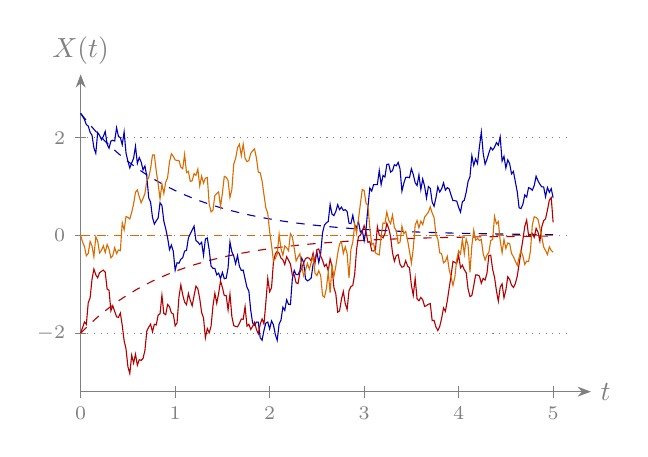
\begin{tikzpicture}[x=1.2cm, y=0.62cm, >=Stealth]
        \draw[->, gray] (0,-3.2) -- (5.4,-3.2) node[right] {$t$};
        \draw[->, gray] (0,-3.2) -- (0,3.3) node[above] {$X(t)$};
        \foreach \v in {-2,0,2} {
            \draw[gray, dotted] (0,\v) -- (5.2,\v);
            \draw[gray] (0.06,\v) -- (-0.06,\v) node[left, font=\scriptsize] {$\v$};
        }
        \foreach \v in {0,...,5}
            \draw[gray] (\v,-3.08) -- (\v,-3.32) node[below, font=\scriptsize] {$\v$};
        \draw[blue!70!black, dashed, thin] plot[domain=0:5, samples=60] (\x, {2.5*exp(-\x)});
        \draw[red!70!black, dashed, thin] plot[domain=0:5, samples=60] (\x, {-2.0*exp(-\x)});
        \draw[orange!85!black, dashed, thin] plot[domain=0:5, samples=60] (\x, {0*exp(-\x)});
        \draw[blue!70!black] plot coordinates {(0.00,2.500) (0.02,2.439) (0.04,2.376) (0.06,2.270) (0.08,2.243) (0.10,2.112) (0.12,2.053) (0.14,1.795) (0.16,1.684) (0.18,2.106) (0.20,2.050) (0.22,1.962) (0.24,2.029) (0.26,2.130) (0.28,1.865) (0.30,1.786) (0.32,1.934) (0.34,1.949) (0.36,1.934) (0.38,2.207) (0.40,2.027) (0.42,2.003) (0.44,1.859) (0.46,2.120) (0.48,1.687) (0.50,1.519) (0.52,1.383) (0.54,1.488) (0.56,1.580) (0.58,1.827) (0.60,1.476) (0.62,1.596) (0.64,1.506) (0.66,1.342) (0.68,1.423) (0.70,1.211) (0.72,0.771) (0.74,0.682) (0.76,0.369) (0.78,0.232) (0.80,0.301) (0.82,0.358) (0.84,0.668) (0.86,0.615) (0.88,0.296) (0.90,0.138) (0.92,-0.048) (0.94,-0.291) (0.96,-0.198) (0.98,-0.323) (1.00,-0.712) (1.02,-0.558) (1.04,-0.570) (1.06,-0.487) (1.08,-0.456) (1.10,-0.320) (1.12,-0.306) (1.14,-0.053) (1.16,0.033) (1.18,0.111) (1.20,0.191) (1.22,-0.105) (1.24,-0.135) (1.26,-0.185) (1.28,-0.139) (1.30,-0.408) (1.32,-0.073) (1.34,-0.051) (1.36,-0.292) (1.38,-0.628) (1.40,-0.672) (1.42,-0.676) (1.44,-0.807) (1.46,-0.772) (1.48,-0.885) (1.50,-0.757) (1.52,-0.887) (1.54,-0.876) (1.56,-0.663) (1.58,-0.136) (1.60,-0.334) (1.62,-0.421) (1.64,-0.580) (1.66,-0.412) (1.68,-0.633) (1.70,-0.717) (1.72,-0.709) (1.74,-0.890) (1.76,-1.064) (1.78,-1.138) (1.80,-1.535) (1.82,-1.794) (1.84,-1.840) (1.86,-1.774) (1.88,-1.776) (1.90,-2.095) (1.92,-2.146) (1.94,-1.943) (1.96,-1.793) (1.98,-1.773) (2.00,-1.915) (2.02,-1.750) (2.04,-1.831) (2.06,-2.028) (2.08,-2.148) (2.10,-1.816) (2.12,-1.735) (2.14,-1.469) (2.16,-1.535) (2.18,-1.317) (2.20,-1.411) (2.22,-1.414) (2.24,-0.889) (2.26,-0.717) (2.28,-0.803) (2.30,-0.804) (2.32,-0.723) (2.34,-0.466) (2.36,-0.555) (2.38,-0.892) (2.40,-0.930) (2.42,-0.908) (2.44,-0.868) (2.46,-0.588) (2.48,-0.513) (2.50,-0.340) (2.52,-0.553) (2.54,-0.368) (2.56,0.058) (2.58,0.212) (2.60,0.258) (2.62,0.284) (2.64,0.635) (2.66,0.437) (2.68,0.406) (2.70,0.490) (2.72,0.629) (2.74,0.529) (2.76,0.580) (2.78,0.513) (2.80,0.527) (2.82,0.490) (2.84,0.252) (2.86,0.242) (2.88,0.413) (2.90,0.211) (2.92,0.159) (2.94,0.289) (2.96,0.069) (2.98,0.104) (3.00,-0.110) (3.02,0.119) (3.04,0.579) (3.06,0.972) (3.08,0.909) (3.10,1.039) (3.12,1.042) (3.14,1.042) (3.16,1.330) (3.18,1.040) (3.20,1.230) (3.22,1.196) (3.24,1.454) (3.26,1.462) (3.28,1.298) (3.30,1.328) (3.32,1.448) (3.34,1.427) (3.36,1.496) (3.38,1.361) (3.40,0.907) (3.42,1.069) (3.44,1.188) (3.46,1.194) (3.48,1.183) (3.50,1.367) (3.52,1.248) (3.54,1.082) (3.56,1.023) (3.58,1.240) (3.60,0.938) (3.62,1.157) (3.64,1.006) (3.66,0.766) (3.68,1.003) (3.70,0.963) (3.72,0.684) (3.74,0.599) (3.76,0.773) (3.78,0.996) (3.80,0.890) (3.82,0.954) (3.84,1.078) (3.86,0.927) (3.88,0.980) (3.90,0.954) (3.92,0.827) (3.94,0.712) (3.96,0.712) (3.98,0.703) (4.00,0.576) (4.02,0.479) (4.04,0.692) (4.06,0.721) (4.08,0.884) (4.10,1.107) (4.12,1.202) (4.14,1.632) (4.16,1.435) (4.18,1.568) (4.20,1.473) (4.22,1.814) (4.24,2.118) (4.26,1.685) (4.28,1.458) (4.30,1.561) (4.32,1.688) (4.34,1.802) (4.36,1.751) (4.38,1.807) (4.40,1.902) (4.42,1.848) (4.44,2.017) (4.46,1.524) (4.48,1.621) (4.50,1.382) (4.52,1.546) (4.54,1.469) (4.56,1.262) (4.58,1.311) (4.60,1.103) (4.62,0.898) (4.64,0.567) (4.66,0.550) (4.68,0.639) (4.70,0.830) (4.72,0.785) (4.74,0.979) (4.76,0.963) (4.78,0.925) (4.80,1.022) (4.82,1.213) (4.84,1.120) (4.86,1.049) (4.88,0.996) (4.90,0.993) (4.92,0.793) (4.94,0.982) (4.96,0.883) (4.98,0.958) (5.00,0.773)};
        \draw[red!70!black] plot coordinates {(0.00,-2.000) (0.02,-1.888) (0.04,-1.772) (0.06,-1.821) (0.08,-1.380) (0.10,-1.278) (0.12,-0.897) (0.14,-0.688) (0.16,-0.806) (0.18,-0.867) (0.20,-0.762) (0.22,-0.735) (0.24,-0.710) (0.26,-0.753) (0.28,-1.100) (0.30,-1.123) (0.32,-1.544) (0.34,-1.439) (0.36,-1.555) (0.38,-1.667) (0.40,-1.678) (0.42,-1.590) (0.44,-1.844) (0.46,-2.157) (0.48,-2.327) (0.50,-2.689) (0.52,-2.829) (0.54,-2.454) (0.56,-2.616) (0.58,-2.433) (0.60,-2.659) (0.62,-2.546) (0.64,-2.559) (0.66,-2.520) (0.68,-2.356) (0.70,-1.957) (0.72,-1.879) (0.74,-1.817) (0.76,-1.975) (0.78,-1.819) (0.80,-1.832) (0.82,-1.629) (0.84,-1.605) (0.86,-1.225) (0.88,-1.597) (0.90,-1.624) (0.92,-1.415) (0.94,-1.457) (0.96,-1.586) (0.98,-1.608) (1.00,-1.852) (1.02,-1.791) (1.04,-1.267) (1.06,-1.013) (1.08,-1.214) (1.10,-1.365) (1.12,-1.418) (1.14,-1.189) (1.16,-1.330) (1.18,-1.441) (1.20,-1.235) (1.22,-1.038) (1.24,-1.092) (1.26,-1.293) (1.28,-1.577) (1.30,-1.686) (1.32,-2.098) (1.34,-1.906) (1.36,-1.994) (1.38,-1.858) (1.40,-1.447) (1.42,-1.184) (1.44,-1.390) (1.46,-1.188) (1.48,-0.933) (1.50,-1.064) (1.52,-1.233) (1.54,-1.230) (1.56,-1.526) (1.58,-1.201) (1.60,-1.658) (1.62,-1.847) (1.64,-1.864) (1.66,-1.872) (1.68,-1.801) (1.70,-1.711) (1.72,-1.719) (1.74,-1.457) (1.76,-1.856) (1.78,-1.819) (1.80,-1.926) (1.82,-1.861) (1.84,-1.779) (1.86,-1.926) (1.88,-2.016) (1.90,-1.817) (1.92,-1.711) (1.94,-1.813) (1.96,-1.368) (1.98,-0.879) (2.00,-1.154) (2.02,-1.071) (2.04,-0.547) (2.06,-0.380) (2.08,-0.328) (2.10,-0.363) (2.12,-0.464) (2.14,-0.497) (2.16,-0.597) (2.18,-0.436) (2.20,-0.507) (2.22,-0.585) (2.24,-0.814) (2.26,-0.808) (2.28,-0.970) (2.30,-0.987) (2.32,-0.759) (2.34,-0.671) (2.36,-0.556) (2.38,-0.474) (2.40,-0.453) (2.42,-0.469) (2.44,-0.521) (2.46,-0.359) (2.48,-0.569) (2.50,-0.289) (2.52,-0.277) (2.54,-0.421) (2.56,-0.510) (2.58,-0.635) (2.60,-0.591) (2.62,-0.722) (2.64,-0.480) (2.66,-0.626) (2.68,-1.068) (2.70,-1.193) (2.72,-1.571) (2.74,-1.547) (2.76,-1.305) (2.78,-1.149) (2.80,-1.394) (2.82,-1.518) (2.84,-1.132) (2.86,-1.046) (2.88,-1.024) (2.90,-0.792) (2.92,-0.286) (2.94,-0.021) (2.96,0.007) (2.98,0.078) (3.00,0.200) (3.02,0.074) (3.04,-0.140) (3.06,-0.126) (3.08,-0.313) (3.10,-0.319) (3.12,-0.294) (3.14,0.180) (3.16,0.007) (3.18,-0.018) (3.20,-0.050) (3.22,0.038) (3.24,0.247) (3.26,0.144) (3.28,-0.024) (3.30,-0.351) (3.32,-0.529) (3.34,-0.412) (3.36,-0.394) (3.38,-0.589) (3.40,-0.652) (3.42,-0.633) (3.44,-0.519) (3.46,-0.628) (3.48,-0.665) (3.50,-1.016) (3.52,-1.226) (3.54,-0.878) (3.56,-1.298) (3.58,-1.339) (3.60,-1.269) (3.62,-1.318) (3.64,-1.453) (3.66,-1.437) (3.68,-1.409) (3.70,-1.397) (3.72,-1.745) (3.74,-1.739) (3.76,-1.875) (3.78,-1.948) (3.80,-1.863) (3.82,-1.698) (3.84,-1.484) (3.86,-1.554) (3.88,-1.338) (3.90,-1.077) (3.92,-0.828) (3.94,-0.533) (3.96,-0.552) (3.98,-0.576) (4.00,-0.399) (4.02,-0.664) (4.04,-0.609) (4.06,-0.703) (4.08,-0.763) (4.10,-1.096) (4.12,-1.252) (4.14,-1.231) (4.16,-1.029) (4.18,-0.810) (4.20,-0.810) (4.22,-0.832) (4.24,-0.981) (4.26,-0.881) (4.28,-0.913) (4.30,-0.774) (4.32,-0.408) (4.34,-0.406) (4.36,-0.697) (4.38,-0.856) (4.40,-1.130) (4.42,-1.347) (4.44,-1.059) (4.46,-0.992) (4.48,-1.277) (4.50,-1.120) (4.52,-0.846) (4.54,-0.901) (4.56,-1.018) (4.58,-1.065) (4.60,-0.987) (4.62,-0.839) (4.64,-0.586) (4.66,-0.332) (4.68,-0.088) (4.70,0.186) (4.72,0.315) (4.74,0.002) (4.76,-0.024) (4.78,0.039) (4.80,-0.038) (4.82,0.145) (4.84,0.070) (4.86,-0.117) (4.88,0.174) (4.90,0.304) (4.92,0.342) (4.94,0.520) (4.96,0.723) (4.98,0.776) (5.00,0.269)};
        \draw[orange!85!black] plot coordinates {(0.00,0.000) (0.02,-0.135) (0.04,-0.224) (0.06,-0.416) (0.08,-0.368) (0.10,-0.122) (0.12,-0.217) (0.14,-0.439) (0.16,-0.025) (0.18,-0.115) (0.20,-0.359) (0.22,-0.304) (0.24,-0.213) (0.26,-0.350) (0.28,-0.185) (0.30,-0.279) (0.32,-0.458) (0.34,-0.413) (0.36,-0.250) (0.38,-0.372) (0.40,-0.299) (0.42,-0.311) (0.44,0.260) (0.46,0.113) (0.48,0.388) (0.50,0.369) (0.52,0.337) (0.54,0.474) (0.56,0.643) (0.58,0.884) (0.60,0.932) (0.62,0.793) (0.64,0.670) (0.66,0.758) (0.68,0.859) (0.70,1.122) (0.72,1.183) (0.74,1.372) (0.76,1.647) (0.78,1.647) (0.80,1.317) (0.82,1.055) (0.84,0.747) (0.86,1.050) (0.88,0.859) (0.90,1.089) (0.92,1.184) (0.94,1.503) (0.96,1.674) (0.98,1.620) (1.00,1.548) (1.02,1.534) (1.04,1.538) (1.06,1.401) (1.08,1.367) (1.10,1.661) (1.12,1.287) (1.14,1.313) (1.16,1.106) (1.18,1.121) (1.20,1.267) (1.22,1.230) (1.24,1.360) (1.26,1.015) (1.28,1.216) (1.30,1.071) (1.32,1.174) (1.34,1.187) (1.36,0.646) (1.38,0.482) (1.40,0.516) (1.42,0.817) (1.44,0.858) (1.46,0.892) (1.48,0.592) (1.50,0.866) (1.52,1.210) (1.54,1.192) (1.56,1.124) (1.58,0.778) (1.60,0.939) (1.62,1.461) (1.64,1.575) (1.66,1.796) (1.68,1.869) (1.70,1.634) (1.72,1.869) (1.74,1.585) (1.76,1.511) (1.78,1.536) (1.80,1.682) (1.82,1.732) (1.84,1.774) (1.86,1.587) (1.88,1.297) (1.90,1.283) (1.92,1.116) (1.94,0.832) (1.96,0.562) (1.98,0.453) (2.00,0.073) (2.02,-0.198) (2.04,-0.521) (2.06,-0.474) (2.08,-0.383) (2.10,0.026) (2.12,-0.274) (2.14,-0.404) (2.16,-0.214) (2.18,-0.253) (2.20,-0.313) (2.22,0.035) (2.24,-0.033) (2.26,-0.264) (2.28,-0.522) (2.30,-0.445) (2.32,-0.375) (2.34,-0.641) (2.36,-0.826) (2.38,-0.702) (2.40,-0.573) (2.42,-0.690) (2.44,-0.552) (2.46,-0.426) (2.48,-0.774) (2.50,-0.821) (2.52,-0.722) (2.54,-0.822) (2.56,-1.233) (2.58,-1.265) (2.60,-1.090) (2.62,-0.752) (2.64,-1.175) (2.66,-0.629) (2.68,-0.842) (2.70,-0.633) (2.72,-0.374) (2.74,-0.170) (2.76,-0.136) (2.78,-0.366) (2.80,-0.233) (2.82,-0.372) (2.84,-0.869) (2.86,-0.286) (2.88,-0.138) (2.90,0.228) (2.92,0.041) (2.94,0.334) (2.96,0.645) (2.98,0.943) (3.00,0.920) (3.02,0.661) (3.04,0.612) (3.06,0.160) (3.08,-0.184) (3.10,-0.162) (3.12,-0.357) (3.14,-0.383) (3.16,-0.397) (3.18,-0.003) (3.20,0.257) (3.22,0.243) (3.24,0.480) (3.26,0.314) (3.28,0.240) (3.30,0.418) (3.32,0.161) (3.34,0.102) (3.36,-0.164) (3.38,-0.137) (3.40,0.192) (3.42,0.038) (3.44,0.082) (3.46,-0.099) (3.48,-0.327) (3.50,-0.568) (3.52,-0.265) (3.54,0.212) (3.56,0.305) (3.58,0.155) (3.60,0.293) (3.62,0.221) (3.64,0.376) (3.66,0.427) (3.68,0.475) (3.70,0.586) (3.72,0.459) (3.74,0.369) (3.76,0.017) (3.78,-0.072) (3.80,-0.355) (3.82,-0.376) (3.84,-0.560) (3.86,-0.529) (3.88,-0.428) (3.90,-0.703) (3.92,-0.852) (3.94,-1.023) (3.96,-0.854) (3.98,-0.495) (4.00,-0.315) (4.02,-0.379) (4.04,-0.078) (4.06,-0.379) (4.08,-0.072) (4.10,-0.202) (4.12,-0.754) (4.14,-0.208) (4.16,0.111) (4.18,-0.097) (4.20,-0.062) (4.22,-0.103) (4.24,-0.081) (4.26,-0.376) (4.28,-0.505) (4.30,-0.401) (4.32,-0.348) (4.34,-0.102) (4.36,-0.084) (4.38,0.388) (4.40,0.237) (4.42,0.284) (4.44,-0.105) (4.46,-0.353) (4.48,-0.081) (4.50,-0.267) (4.52,-0.156) (4.54,-0.165) (4.56,-0.371) (4.58,-0.433) (4.60,-0.527) (4.62,-0.614) (4.64,-0.451) (4.66,-0.312) (4.68,-0.421) (4.70,-0.594) (4.72,-0.526) (4.74,-0.535) (4.76,-0.319) (4.78,0.219) (4.80,0.383) (4.82,0.368) (4.84,0.327) (4.86,0.149) (4.88,-0.036) (4.90,-0.236) (4.92,-0.310) (4.94,-0.389) (4.96,-0.233) (4.98,-0.308) (5.00,-0.341)};
    \end{tikzpicture}
    \caption{Left: three paths of Brownian motion, simulated with $h = 0.02$. Right: three paths of the Ornstein--Uhlenbeck process $dX = -X\,dt + \sqrt{2}\,dB$, started at $2.5$, $-2$ and $0$, together with the solutions $X(0)e^{-t}$ of the ODE without noise (dashed). The process forgets its starting point and fluctuates around $0$ with the stationary distribution $\mathcal{N}(0, 1)$; about $95\%$ of the time, it stays between $-2$ and $2$.}
    \label{L4-fig:sde}
\end{figure}

\subsection{Langevin dynamics and diffusion models}\label{L4-sec:langevin}

The Ornstein--Uhlenbeck process is an example of a general principle: a gradient flow with the right amount of noise samples from a probability distribution.

\begin{theorem}[Langevin dynamics]\label{L4-thm:langevin}
    Let $U: \mathbb{R}^d \to \mathbb{R}$ be smooth with $\int e^{-U(\mathbf{x})}\, d\mathbf{x} < \infty$. Then the SDE $d\mathbf{X} = -\nabla U(\mathbf{X})\,dt + \sqrt{2}\,d\mathbf{B}$, where $\mathbf{B}$ is a vector of $d$ independent Brownian motions, has the stationary density $p(\mathbf{x}) \propto e^{-U(\mathbf{x})}$, and under mild conditions, the distribution of $\mathbf{X}(t)$ converges to it.
\end{theorem}

We do not prove the convergence, but we can see why $e^{-U}$ is stationary. Without noise, the density $p_t$ of $\mathbf{X}(t)$ under the flow of the vector field $-\nabla U$ satisfies the continuity equation $\frac{\partial p_t}{\partial t} = -\Div(-p_t\nabla U)$ (Proposition~\ref{L3-prop:continuity}). The noise adds a diffusion term, and one can show that $p_t$ satisfies the Fokker--Planck equation
\[\frac{\partial p_t}{\partial t} = \Div(p_t\nabla U) + \Delta p_t = \Div(p_t\nabla U + \nabla p_t),\]
with the Laplacian $\Delta p_t = \Div\nabla p_t$ (Lecture~3). For $p \propto e^{-U}$, we have $\nabla p = -p\nabla U$, so the right side vanishes, and $p$ does not change in time. For $U = 0$, the Fokker--Planck equation is the heat equation $\frac{\partial p_t}{\partial t} = \Delta p_t$, which describes how the density of $\sqrt{2}\,\mathbf{B}(t)$ spreads out. For $U(x) = \frac{x^2}{2s^2}$, the SDE is the Ornstein--Uhlenbeck process with $\theta = \frac{1}{s^2}$ and $\sigma = \sqrt{2}$, whose stationary variance $\frac{\sigma^2}{2\theta} = s^2$ agrees with the density $e^{-U} \propto e^{-x^2/(2s^2)}$ of $\mathcal{N}(0, s^2)$. The Euler--Maruyama scheme gives the unadjusted Langevin algorithm
\[\mathbf{x}_{k+1} = \mathbf{x}_k - h\nabla U(\mathbf{x}_k) + \sqrt{2h}\,\mathbf{z}_k, \qquad \mathbf{z}_k \sim \mathcal{N}(\mathbf{0}, I),\]
which is gradient descent on $U$ plus Gaussian noise. To sample from a posterior $p(\boldsymbol{\theta} \mid \mathcal{D}) \propto e^{-U(\boldsymbol{\theta})}$, we take $U(\boldsymbol{\theta}) = -\log p(\mathcal{D} \mid \boldsymbol{\theta}) - \log p(\boldsymbol{\theta})$, the training loss plus the regularizer. Without the noise, the iteration converges to the MAP estimate; with the noise, it explores the posterior. The discretization introduces a small bias: for the target $\mathcal{N}(2, 0.25)$ and $h = 0.01$, the stationary variance of the algorithm is $0.2551$ instead of $0.25$, by Example~\ref{L4-ex:ou}. The Metropolis-adjusted Langevin algorithm removes this bias by accepting or rejecting each step as in Theorem~\ref{L4-thm:metropolis}, and stochastic gradient Langevin dynamics uses mini-batch gradients to make the method feasible for large models.

\begin{remark}[SDEs in machine learning]
    \begin{enumerate}
        \item Diffusion models for image generation use an SDE of Ornstein--Uhlenbeck type that gradually turns images into Gaussian noise. The time-reversed process is again an SDE, whose drift involves the score $\nabla\log p_t(\mathbf{x})$ of the noised data distribution at time $t$. A neural network learns this score, with a variant of the score matching loss of Lecture~3, and new images are generated by simulating the reverse SDE, starting from pure noise.
        \item The noise of mini-batch gradients makes SGD with a small step size behave approximately like the Euler--Maruyama scheme for an SDE $d\boldsymbol{\theta} = -\nabla L(\boldsymbol{\theta})\,dt + \sqrt{\eta\,\Sigma(\boldsymbol{\theta})}\,d\mathbf{B}$, where $\Sigma$ is the covariance matrix of the mini-batch gradients. This heuristic is used to study which minima SGD prefers.
    \end{enumerate}
\end{remark}

\section{Key Takeaways}
\begin{itemize}[leftmargin=*]
    \item Probability theory is built on measure theory: events form a $\sigma$-algebra, a probability is a countably additive measure with $P(\Omega) = 1$, and random variables are measurable functions, described by their distributions, or equivalently by their CDFs; $F^{-1}(U)$ with the quantile function $F^{-1}$ samples from the CDF $F$. Probabilities are continuous along increasing and decreasing sequences of events, and null events can happen. Conditional probability $P(A \mid B) = \frac{P(A \cap B)}{P(B)}$ and Bayes' theorem $P(B \mid A) = \frac{P(A \mid B)P(B)}{P(A)}$ update beliefs with evidence; ignoring the prior $P(B)$ is the base rate fallacy.
    \item The expectation is the Lebesgue integral $\E[X] = \int X\, dP$, computed from the distribution as $\E[g(X)] = \sum_i g(x_i)p(x_i)$ or $\int g(x)p(x)\, dx$. Monotone and dominated convergence allow us to exchange limits and expectations, and to differentiate under the integral sign; without a dominating function, mass can escape. Pmfs and pdfs are densities with respect to the counting and the Lebesgue measure (Radon--Nikodym), and mixed distributions such as the ReLU of a Gaussian have densities with respect to other measures.
    \item The expectation is linear; $\Var(X) = \E[X^2] - \E[X]^2$; Markov's, Chebyshev's, Chernoff's and Jensen's inequalities relate them. For densities, $p_Y(y) = \frac{p_X(x)}{|g'(x)|}$ under $y = g(x)$.
    \item The sum rule $p(x) = \sum_y p(x, y)$ and the product rule $p(x, y) = p(y \mid x)p(x)$ are the basic rules of probabilistic modeling. Independence means that the joint distribution is the product of the marginals; by Fubini--Tonelli, expectations of products of independent random variables factorize, and sums of independent random variables have the convolution of their densities.
    \item Covariance is an inner product on centered random variables, and correlation is the cosine of their angle, so $|\Corr| \leq 1$. Uncorrelated does not imply independent. The conditional expectation $\E[Y \mid \mathcal{G}]$ is the orthogonal projection of $Y$ onto the $\mathcal{G}$-measurable random variables in $L^2$, the best mean-squared-error prediction of $Y$ from the information $\mathcal{G}$; it satisfies the tower property and the law of total variance.
    \item A martingale is a fair game, $\E[M_{n+1} \mid \mathcal{F}_n] = M_n$; random walks, posterior means and likelihood ratios are martingales. Stopping at a stopping time does not change the expectation if the stopped martingale stays bounded (optional stopping), which solves the gambler's ruin, and Ville's inequality gives likelihood ratio tests that stay valid when we look at the data repeatedly.
    \item The covariance matrix $\Sigma = \E[(\mathbf{X} - \boldsymbol{\mu})(\mathbf{X} - \boldsymbol{\mu})^\top]$ is symmetric positive semidefinite, $\Cov(A\mathbf{X} + \mathbf{b}) = A\Sigma A^\top$, and $\Var(\mathbf{u}^\top\mathbf{X}) = \mathbf{u}^\top\Sigma\mathbf{u}$ is maximal for the top eigenvector (PCA). Whitening $\Sigma^{-1/2}(\mathbf{X} - \boldsymbol{\mu})$ gives identity covariance.
    \item $\mathcal{N}(\boldsymbol{\mu}, \Sigma)$ is the distribution of $\boldsymbol{\mu} + A\mathbf{Z}$ with $AA^\top = \Sigma$ and $\mathbf{Z} \sim \mathcal{N}(\mathbf{0}, I)$; its level sets are ellipsoids along the eigenvectors of $\Sigma$. Affine maps, marginals and conditionals of Gaussians are Gaussian, with $\mathbf{X}_a \mid \mathbf{x}_b \sim \mathcal{N}\big(\boldsymbol{\mu}_a + \Sigma_{ab}\Sigma_{bb}^{-1}(\mathbf{x}_b - \boldsymbol{\mu}_b), \Sigma_{aa} - \Sigma_{ab}\Sigma_{bb}^{-1}\Sigma_{ba}\big)$; for jointly Gaussian vectors, uncorrelated means independent.
    \item The sample mean of $N$ i.i.d.\ variables has standard error $\frac{\sigma}{\sqrt{N}}$; it converges to $\mu$ in probability (weak law) and almost surely (strong law), its fluctuations are approximately Gaussian (central limit theorem), and for bounded variables Hoeffding's inequality bounds large deviations exponentially. Almost sure convergence and convergence in $L^p$ imply convergence in probability, which implies convergence in distribution, but not conversely; the Borel--Cantelli lemma proves almost sure statements, and Slutsky's theorem and the delta method carry limits in distribution over to estimated standard errors and to smooth functions of estimators.
    \item Averages of samples underlie Monte Carlo methods, test set evaluation, and stochastic gradients. Rejection sampling draws exact samples using an envelope $p \leq Mq$ (acceptance rate $\frac{1}{M}$); importance sampling reweights samples from $q$ by the likelihood ratio $\frac{p}{q}$, which can reduce the variance dramatically for rare events.
    \item A Markov chain with transition matrix $P$ evolves by $\boldsymbol{\pi}_{t+1} = \boldsymbol{\pi}_t P$. Stationary distributions are left eigenvectors of $P$ with eigenvalue $1$; an irreducible, aperiodic chain converges to its unique stationary distribution, at a speed governed by the second largest eigenvalue in absolute value. Detailed balance $\pi_i P_{ij} = \pi_j P_{ji}$ implies stationarity; the Metropolis algorithm uses it to sample from distributions that are only known up to a constant (MCMC).
    \item Estimators have a bias and a variance, and $\mathrm{MSE} = \text{bias}^2 + \text{variance}$, so some bias (shrinkage) can pay off; if both tend to $0$, the estimator is consistent. The sample variance needs the factor $\frac{1}{N - 1}$ to be unbiased. No unbiased estimator has a variance below the Cram\'er--Rao bound $\frac{1}{N\,I(\theta)}$, where the Fisher information $I(\theta)$ is the variance of the score $\frac{\partial}{\partial\theta}\log p(x \mid \theta)$; the MLE attains it asymptotically, and its standard error is estimated from the curvature of the log-likelihood. A sufficient statistic carries all the information about $\theta$, and conditioning an estimator on it never increases the MSE (Rao--Blackwell).
    \item Maximum likelihood maximizes $\sum_i \log p(x_i \mid \theta)$. Least squares is maximum likelihood with Gaussian noise, and the cross-entropy loss is maximum likelihood for categorical labels; the MLE of a Gaussian is the sample mean and the (biased) sample covariance. The method of moments matches sample moments instead; it is simpler but usually less efficient. Confidence intervals $\bar x \pm 1.96\frac{s}{\sqrt{N}}$ quantify uncertainty.
    \item A test rejects $H_0$ if the p-value, the probability under $H_0$ of data at least as extreme as observed, is at most $\alpha$; under $H_0$, p-values are uniform, so the false positive rate is $\alpha$, and the power is the probability of detecting a real effect. A p-value is not the probability that $H_0$ is true. Paired $t$-tests compare two models on the same data sets, and Pearson's $\chi^2$ test compares observed counts with expected counts. Many tests need corrections: Bonferroni ($\frac{\alpha}{m}$) controls the family-wise error rate, Benjamini--Hochberg the false discovery rate. The bootstrap (resampling the data with replacement) estimates standard errors of any statistic, and permutation tests (relabeling the groups) give exact p-values without distributional assumptions.
    \item Cross-validation estimates the generalization error, but its naive standard error is too small, and the best of many cross-validated models is optimistically biased; compare models with paired differences and evaluate the final choice on untouched data. A/B tests randomize to measure causal effects; plan the sample size $n \approx (z_{1-\alpha/2} + z_{1-\beta})^2\,2\bar p(1 - \bar p)/\delta^2$ per group in advance, and do not stop at the first significant peek.
    \item Bayesian inference updates a prior to the posterior $p(\theta \mid \mathcal{D}) \propto p(\mathcal{D} \mid \theta)p(\theta)$. Conjugate priors (Beta for Bernoulli, Gamma for Poisson, Gaussian for linear regression) give closed-form posteriors, and credible intervals are quantiles of the posterior. MAP estimation adds the regularizer $-\log p(\theta)$: a Gaussian prior gives ridge regression, a Laplace prior the lasso. The Bayesian posterior also gives predictive uncertainty. A Gaussian process is a prior on functions given by a kernel; its posterior follows from Gaussian conditioning, with the mean $\mathbf{k}_*^\top(K + \sigma^2I)^{-1}\mathbf{y}$ and a variance that is small near the data.
    \item Entropy measures uncertainty, cross-entropy $H(p, q) = H(p) + \KL(p \,\|\, q)$, and $\KL(p \,\|\, q) \geq 0$ with equality only for $p = q$ (Gibbs). Maximum likelihood minimizes the cross-entropy and the KL divergence from the empirical distribution to the model. Among all densities with a given variance, the Gaussian has the largest entropy.
    \item Brownian motion has independent Gaussian increments $B(t) - B(s) \sim \mathcal{N}(0, t - s)$ and continuous, nowhere differentiable paths, and it is a martingale. An SDE $dX = \mu(X)\,dt + \sigma(X)\,dB$ is simulated by Euler--Maruyama, $X_{k+1} = X_k + \mu(X_k)h + \sigma(X_k)\sqrt{h}\,Z_k$: noise of size $\sqrt{h}$, not $h$. Langevin dynamics $d\mathbf{X} = -\nabla U\,dt + \sqrt{2}\,d\mathbf{B}$ samples from $p \propto e^{-U}$, the stationary solution of the Fokker--Planck equation; its discretization is gradient descent plus noise, and diffusion models generate data by reversing a noising SDE.
\end{itemize}

\section{Exercises}\label{L4-sec:exercises}
\begin{enumerate}[leftmargin=*]
    \item ($\sigma$-algebras.)
    \begin{enumerate}[label=(\alph*)]
        \item Show that the intersection of two $\sigma$-algebras on $\Omega$ is a $\sigma$-algebra, but that their union need not be one. (Hint: $\Omega = \{1, 2, 3\}$.)
        \item Let $\mathcal{G}$ be the $\sigma$-algebra on $\Omega = \{1, \ldots, 6\}^2$ generated by the events $\{\text{the sum is } s\}$ for two dice. How many elements does $\mathcal{G}$ have? Does it contain the event ``both dice show the same number''?
    \end{enumerate}
    \item (The birthday problem.) Assume that birthdays are independent and uniformly distributed over $365$ days. Show that the probability that among $n$ people at least two share a birthday is $1 - \frac{365 \cdot 364 \cdots (365 - n + 1)}{365^n}$, and that it exceeds $\frac{1}{2}$ for $n = 23$. How many people are needed for $99\%$?
    \item \begin{enumerate}[label=(\alph*)]
        \item Prove the inclusion--exclusion formula $P(A \cup B \cup C) = P(A) + P(B) + P(C) - P(A \cap B) - P(A \cap C) - P(B \cap C) + P(A \cap B \cap C)$.
        \item Two fair coins are flipped. Let $A$ = ``the first coin shows heads'', $B$ = ``the second coin shows heads'', and $C$ = ``exactly one coin shows heads''. Show that any two of these events are independent, but the three events are not independent.
    \end{enumerate}
    \item A spam filter knows that $40\%$ of all emails are spam, that the word ``free'' appears in $30\%$ of the spam emails and in $2\%$ of the other emails. What is the probability that an email containing ``free'' is spam?
    \item Let $X$ be a random variable with the CDF $F$. Use the continuity of probability to show that $P(X > t) \to 0$ as $t \to \infty$, and that $P(X = x) = F(x) - \lim_{y \uparrow x} F(y)$. Conclude that $F$ has at most countably many jumps. (Hint: there are at most $n$ jumps of size larger than $\frac{1}{n}$.)
    \item Let $X$ be Geometric$(p)$. Show that $\E[X] = \frac{1}{p}$ and that $P(X > s + t \mid X > s) = P(X > t)$ for all positive integers $s$ and $t$. How many times do you expect to roll a fair die until you see a six?
    \item Let $U$ and $V$ be independent and Uniform$(0, 1)$. Find the densities of (a) $U^2$, (b) $-\log U$, (c) $\max(U, V)$ (Hint: compute the CDF first.)
    \item Let $X$ be Poisson$(\lambda)$. Compute $\E[X(X - 1)]$, and use it to show that $\Var(X) = \lambda$.
    \item (Limits and expectations.)
    \begin{enumerate}[label=(\alph*)]
        \item Use monotone convergence to show that $\lim_{n \to \infty}\int_0^n \big(1 - \frac{x}{n}\big)^n\, dx = 1$. (Hint: $(1 - \frac{x}{n})^n\mathbf{1}_{[0, n]}(x)$ increases to $e^{-x}$.)
        \item Let $X \geq 0$ with $\E[X] < \infty$. Show that $\E[X\mathbf{1}_{\{X > t\}}] \to 0$ as $t \to \infty$, and conclude that $nP(X > n) \to 0$.
        \item Find random variables $X_n \geq 0$ with $X_n \to 0$ almost surely and $\E[X_n] \to \infty$.
    \end{enumerate}
    \item A waiting time $Z \sim$ Exponential$(1)$ is cut off after $2$ minutes: $Y = \min(Z, 2)$. Find the CDF of $Y$ and a density of $Y$ with respect to $\lambda + \delta_2$, and compute $\E[Y]$ in two ways: with this density, and with the tail integral of Example~\ref{L4-ex:tail-integral}.
    \item \begin{enumerate}[label=(\alph*)]
        \item A nonnegative random variable has mean $2$. Bound $P(X \geq 10)$ with Markov's inequality, and compare with the exact value for $X \sim$ Exponential$(\frac{1}{2})$.
        \item Use Jensen's inequality to show that $\E[\frac{1}{X}] \geq \frac{1}{\E[X]}$ for every positive random variable $X$, and that $\E[e^X] \geq e^{\E[X]}$.
    \end{enumerate}
    \item\label{L4-ex4:joint-pmf} Let $(X, Y)$ have the joint pmf $p(0, 0) = 0.1$, $p(0, 1) = 0.2$, $p(0, 2) = 0.1$, $p(1, 0) = 0.2$, $p(1, 1) = 0.1$, $p(1, 2) = 0.3$. Compute the marginal distributions, $\E[Y \mid X = 0]$ and $\E[Y \mid X = 1]$, and check the tower property. Compute $\Cov(X, Y)$. Are $X$ and $Y$ independent?
    \item Let $X \sim \mathcal{N}(0, 1)$. Show that $X$ and $X^2$ are uncorrelated, but not independent. Show that $\Corr(X, aX + b) = \sign(a)$ for $a \neq 0$.
    \item Let $X$ and $Y$ be independent and Exponential$(\lambda)$. Show that $X + Y$ has the density $\lambda^2ze^{-\lambda z}$ for $z > 0$.
    \item Let $X_1$ and $X_2$ be independent and Uniform$(0, 1)$, and $M = \max(X_1, X_2)$. Show that $\E[X_1 \mid M] = \frac{3}{4}M$, and check the tower property. (Hint: given $M = m$, $X_1 = m$ with probability $\frac{1}{2}$, and otherwise $X_1$ is uniform on $[0, m]$.)
    \item (P\'olya's urn.) An urn contains one red and one blue ball. Repeatedly, a ball is drawn at random and put back together with another ball of the same color. Let $R_n$ be the fraction of red balls after $n$ draws. Show that $(R_n)$ is a martingale, and find $\E[R_n]$.
    \item Let $\mathbf{X}$ have the covariance matrix $\Sigma = \begin{pmatrix} 2 & -1 & 0 \\ -1 & 2 & -1 \\ 0 & -1 & 2 \end{pmatrix}$. Compute $\Var(X_1 + X_2 + X_3)$ and $\Var(X_1 - X_3)$. In which direction $\mathbf{u}$ (with $\norm{\mathbf{u}} = 1$) is $\Var(\mathbf{u}^\top\mathbf{X})$ largest, and what is it? Find a matrix $A$ such that $A\mathbf{X}$ has covariance matrix $I$.
    \item Let $(X, Y) \sim \mathcal{N}\Big(\mathbf{0}, \begin{pmatrix} 4 & 2 \\ 2 & 2 \end{pmatrix}\Big)$. Find the conditional distributions of $Y$ given $X = x$ and of $X$ given $Y = y$, the distribution of $X - Y$, and $P(X > Y)$. Describe the level curves of the density.
    \item Let $\mathbf{X} \sim \mathcal{N}(\boldsymbol{\mu}, \Sigma)$ in $\mathbb{R}^d$. Show that the squared Mahalanobis distance $(\mathbf{X} - \boldsymbol{\mu})^\top\Sigma^{-1}(\mathbf{X} - \boldsymbol{\mu})$ has the same distribution as $\norm{\mathbf{Z}}^2$ with $\mathbf{Z} \sim \mathcal{N}(\mathbf{0}, I)$, and that its expectation is $d$. What does this say about where the probability mass of a high-dimensional Gaussian lies?
    \item How many times do we have to flip a fair coin so that the fraction of heads is within $0.01$ of $\frac{1}{2}$ with probability at least $95\%$? Answer with Chebyshev's inequality, with Hoeffding's inequality, and with the central limit theorem, and compare.
    \item Let $X_n$ be independent with $P(X_n = 1) = p_n$ and $P(X_n = 0) = 1 - p_n$.
    \begin{enumerate}[label=(\alph*)]
        \item For $p_n = \frac{1}{n}$, show that $X_n \to 0$ in probability and in $L^1$, but not almost surely.
        \item For $p_n = \frac{1}{n^2}$, show that $X_n \to 0$ almost surely.
    \end{enumerate}
    \item (Delta method.) Let $X_1, \ldots, X_N$ be i.i.d.\ Exponential$(\lambda)$. Show that $\sqrt{N}\big(\frac{1}{\bar X_N} - \lambda\big) \to \mathcal{N}(0, \lambda^2)$ in distribution, and compare with the Fisher information of the exponential distribution (Exercise~\ref{L4-ex4:fisher}).
    \item Let $p(x) = \sqrt{2/\pi}\,e^{-x^2/2}$ for $x > 0$ be the density of $|Z|$ for $Z \sim \mathcal{N}(0, 1)$, and let $q(x) = e^{-x}$ be the Exponential$(1)$ density.
    \begin{enumerate}[label=(\alph*)]
        \item Find the smallest $M$ with $p \leq Mq$, and the acceptance rate of rejection sampling with this proposal.
        \item Write down the importance sampling estimator of $\E_p[X^2]$ with samples from $q$, and explain why its variance is finite.
    \end{enumerate}
    \item Consider the Markov chain with the transition matrix
    \[P = \begin{pmatrix} 0.7 & 0.2 & 0.1 \\ 0.3 & 0.5 & 0.2 \\ 0.2 & 0.3 & 0.5 \end{pmatrix}.\]
    Draw its transition graph, compute $P(X_2 = 3 \mid X_0 = 1)$, and find the stationary distribution. Is the chain irreducible and aperiodic? In the long run, what fraction of the time does it spend in state $1$?
    \item (Random walks on graphs.)
    \begin{enumerate}[label=(\alph*)]
        \item Let the walker of Example~\ref{L4-ex:random-walk-graph} move on the cycle with the four vertices $1, 2, 3, 4$ (and the edges $\{1, 2\}, \{2, 3\}, \{3, 4\}, \{4, 1\}$). Find the stationary distribution and the eigenvalues of $P$. Show that the distribution of $X_t$ does not converge if $X_0 = 1$.
        \item The lazy walk stays at the current vertex with probability $\frac{1}{2}$, i.e., it has the transition matrix $\frac{1}{2}(I + P)$. Show that it has the same stationary distribution, find its eigenvalues, and explain why it converges.
    \end{enumerate}
    \item\label{L4-ex4:uniform-mle} Let $X_1, \ldots, X_N$ be i.i.d.\ Uniform$(0, \theta)$.
    \begin{enumerate}[label=(\alph*)]
        \item Show that the MLE of $\theta$ is $M = \max_i X_i$, and that $\E[M] = \frac{N}{N + 1}\theta$. (Hint: $P(M \leq t) = (t/\theta)^N$.)
        \item Show that $\frac{N + 1}{N}M$ and $2\bar X_N$ are unbiased, and compare their variances, $\frac{\theta^2}{N(N + 2)}$ and $\frac{\theta^2}{3N}$. Which estimator is better?
    \end{enumerate}
    \item Find the maximum likelihood estimates for i.i.d.\ data from (a) Poisson$(\lambda)$, (b) Exponential$(\lambda)$, (c) Geometric$(p)$.
    \item\label{L4-ex4:fisher} (Fisher information.)
    \begin{enumerate}[label=(\alph*)]
        \item Show that the Fisher information of Poisson$(\lambda)$ is $I(\lambda) = \frac{1}{\lambda}$, and that the MLE $\bar X_N$ is efficient.
        \item Show that $I(\lambda) = \frac{1}{\lambda^2}$ for Exponential$(\lambda)$. The sum $S$ of $N \geq 3$ i.i.d.\ Exponential$(\lambda)$ variables has the Gamma density $\frac{\lambda^N s^{N-1}e^{-\lambda s}}{(N - 1)!}$ for $s > 0$. Use it to show that the MLE $\frac{1}{\bar X_N}$ has the expectation $\frac{N\lambda}{N - 1}$, that $\frac{N - 1}{N\bar X_N}$ is unbiased, and that its variance $\frac{\lambda^2}{N - 2}$ is larger than the Cram\'er--Rao bound. Is the MLE asymptotically efficient?
        \item Counts of $N = 50$ independent Poisson observations have the sample mean $3$. Estimate the standard error of $\hat\lambda$ from the observed information $-\ell''(\hat\lambda)$, and give an approximate $95\%$ confidence interval for $\lambda$.
    \end{enumerate}
    \item (Rao--Blackwell.) Let $X_1, \ldots, X_N$ be i.i.d.\ Uniform$(0, \theta)$. One can show that $M = \max_i X_i$ is sufficient for $\theta$. Show that $\E[2X_1 \mid M] = \frac{N + 1}{N}M$: Rao--Blackwellizing the unbiased estimator $2X_1$ gives the unbiased estimator of Exercise~\ref{L4-ex4:uniform-mle}. (Hint: given $M = m$, $X_1 = m$ with probability $\frac{1}{N}$, and otherwise $X_1$ is uniform on $[0, m]$.)
    \item Assume the regression model $y_i = \mathbf{w}^\top\mathbf{x}_i + \varepsilon_i$ with i.i.d.\ Laplace noise, with density $\frac{1}{2b}e^{-|\varepsilon|/b}$. Show that the MLE of $\mathbf{w}$ minimizes $\sum_i |y_i - \mathbf{w}^\top\mathbf{x}_i|$. In the special case $\mathbf{x}_i = 1$ (estimating a single number $w$), show that every median of the $y_i$ is a minimizer.
    \item Find the method of moments estimators of (a) $a$ and $b$ for Uniform$(a, b)$, using the mean and the variance; (b) the shape $k$ and the scale $s$ of a Gamma distribution, for data with the sample mean $4$ and the sample variance $8$.
    \item A die is rolled $120$ times and shows $30$ sixes. Test at the level $0.05$ whether the die favors sixes: state $H_0$ and $H_1$, and compute the exact one-sided p-value $P(S \geq 30)$ for $S \sim$ Binomial$(120, \frac{1}{6})$ with a computer, and its normal approximation.
    \item Out of $200$ users, $70$, $80$ and $50$ prefer the layouts A, B and C. Use Pearson's $\chi^2$ test to test at the level $0.05$ whether the three layouts are equally popular. (The $\chi^2_2$ distribution has the tail $P(\chi^2_2 \geq c) = e^{-c/2}$.)
    \item \begin{enumerate}[label=(\alph*)]
        \item Show that for $m$ independent tests of true null hypotheses at the level $\frac{\alpha}{m}$, the probability of at least one rejection is $1 - (1 - \frac{\alpha}{m})^m \leq \alpha$.
        \item In a permutation test with two groups of three observations each, what is the smallest possible one-sided p-value? What does this mean for very small experiments?
        \item Show that the bootstrap standard error of the sample mean (for $B \to \infty$) is $\frac{\hat\sigma}{\sqrt{N}}$ with $\hat\sigma^2 = \frac{1}{N}\sum_i (x_i - \bar x)^2$.
    \end{enumerate}
    \item An online shop wants to test whether a new design increases the click-through rate from $10\%$ to $11\%$. How many users per group are needed for a two-sided test at the level $0.05$ with power $0.8$? After the experiment, the two groups of $15\,000$ users have $1500$ and $1650$ clicks. Compute the z-statistic, the p-value, and a $95\%$ confidence interval for the difference.
    \item With the uniform prior Beta$(1, 1)$, a coin shows $7$ heads in $10$ flips. Find the posterior distribution, its mean, the MAP estimate, the MLE, and the predictive probability of heads in the next flip.
    \item (Gaussian--Gaussian conjugacy.) Let $x_1, \ldots, x_N$ be i.i.d.\ $\mathcal{N}(\mu, \sigma^2)$ with known $\sigma^2$, and let the prior be $\mu \sim \mathcal{N}(\mu_0, \tau^2)$. Show that the posterior is Gaussian with precision $\frac{1}{\tau^2} + \frac{N}{\sigma^2}$ and mean
    \[\frac{\mu_0/\tau^2 + N\bar x/\sigma^2}{1/\tau^2 + N/\sigma^2},\]
    a weighted average of the prior mean and the sample mean. What happens as $N \to \infty$?
    \item (Gaussian processes and Bayesian linear regression.)
    \begin{enumerate}[label=(\alph*)]
        \item Show that $(X^\top X + \lambda I)X^\top = X^\top(XX^\top + \lambda I)$ for every matrix $X$ and $\lambda > 0$, and conclude that $(X^\top X + \lambda I)^{-1}X^\top = X^\top(XX^\top + \lambda I)^{-1}$.
        \item Use (a) to show that for the linear kernel $k(\mathbf{x}, \mathbf{x}') = \alpha^{-1}\mathbf{x}^\top\mathbf{x}'$, the posterior mean of Proposition~\ref{L4-prop:gp-regression} equals $\mathbf{m}^\top\mathbf{x}_*$ from Theorem~\ref{L4-thm:blr}. Which of the two formulas is cheaper to evaluate when $N \gg d$, and which when $d \gg N$?
        \item Let $f \sim \mathcal{GP}(0, k)$ with $k(s, t) = \min(s, t)$, and observe $f(1) = 1$ without noise. Find the posterior mean and variance of $f(t)$ for $0 \leq t \leq 1$ and for $t > 1$, and sketch them.
    \end{enumerate}
    \item \begin{enumerate}[label=(\alph*)]
        \item Compute the entropy of a fair die in bits.
        \item Compute $\KL(\text{Bernoulli}(p) \,\|\, \text{Bernoulli}(q))$, and show that
        \[\KL\big(\mathcal{N}(\mu_1, \sigma^2) \,\|\, \mathcal{N}(\mu_2, \sigma^2)\big) = \frac{(\mu_1 - \mu_2)^2}{2\sigma^2}.\]
        \item Show that $I(X; Y) = H(X) + H(Y) - H(X, Y)$ for discrete random variables, where $H(X, Y)$ is the entropy of the joint distribution. Compute $I(X; Y)$ for Exercise~\ref{L4-ex4:joint-pmf}.
    \end{enumerate}
    \item (Brownian motion and the Ornstein--Uhlenbeck process.)
    \begin{enumerate}[label=(\alph*)]
        \item Compute $\Var(B(2) - B(0.5))$, $\Cov(B(1), B(3))$ and $\Corr(B(1), B(3))$.
        \item Let $c > 0$. Show that $W(t) = \frac{1}{\sqrt{c}}B(ct)$ has the same mean and covariance functions as $B(t)$. (In fact, $W$ is again a Brownian motion: zooming into a Brownian path by the factor $c$ in time and $\sqrt{c}$ in space gives a Brownian path.)
        \item Let $X_{k+1} = (1 - \theta h)X_k + \sigma\sqrt{h}\,Z_k$ with $X_0 = x_0$ and i.i.d.\ $Z_k \sim \mathcal{N}(0, 1)$. Show that $\E[X_k] = (1 - \theta h)^kx_0$ and $\Var(X_k) = v_h\big(1 - (1 - \theta h)^{2k}\big)$, with $v_h$ from Example~\ref{L4-ex:ou}. What happens for $\theta h > 2$?
    \end{enumerate}
\end{enumerate}

\section{Programming Exercises}\label{L4-sec:programming}

% Inline code cannot be hyphenated, so allow a little extra stretch in this section.
\setlength{\emergencystretch}{3em}

As in the previous lectures, implement the methods yourself with NumPy, and use library routines (such as \py{rng.normal} or \py{scipy.stats}) only to check your results. Start each file with
\begin{lstlisting}
import numpy as np
import matplotlib.pyplot as plt
rng = np.random.default_rng(0)
\end{lstlisting}

\begin{enumerate}[label=\textbf{P\arabic*.}, leftmargin=*]
    \item \textbf{Monte Carlo estimation.} Estimate $\pi$ from $N$ uniform random points in $[-1, 1]^2$, for $N = 10^2, 10^3, \ldots, 10^7$. Plot the absolute error against $N$ on a log-log scale, together with the standard error $4\sqrt{\frac{\pi}{4}(1 - \frac{\pi}{4})/N}$. What is the slope? Then estimate the volume of the unit ball in $\mathbb{R}^d$ for $d = 2, 5, 10, 20$ in the same way. What goes wrong in high dimensions?

    \item \textbf{Sampling.} Generate $10^5$ samples from each of the following distributions, using only \py{rng.random()} (uniform samples), and compare histograms with the densities.
    \begin{itemize}
        \item Exponential$(\lambda)$ by inverse transform sampling (Theorem~\ref{L4-thm:inverse-transform}).
        \item $\mathcal{N}(0, 1)$ with the Box--Muller method: for independent $U_1, U_2 \sim$ Uniform$(0, 1)$, the numbers $\sqrt{-2\log U_1}\cos(2\pi U_2)$ and $\sqrt{-2\log U_1}\sin(2\pi U_2)$ are independent standard normal.
        \item $\mathcal{N}(\boldsymbol{\mu}, \Sigma)$ in $\mathbb{R}^2$ with $\Sigma = \begin{pmatrix} 3 & 1 \\ 1 & 3 \end{pmatrix}$, via $\boldsymbol{\mu} + L\mathbf{z}$ with the Cholesky factor $L$. Plot the samples together with the ellipses of Figure~\ref{L4-fig:gaussian}, and check the sample mean and covariance matrix. What fraction of the samples lies inside the ellipse with $r = 1$, and with $r = 2$? (Compare with $1 - e^{-r^2/2}$.)
    \end{itemize}

    \item \textbf{Distributions without densities.}
    \begin{itemize}
        \item Implement the quantile function $F^{-1}(u) = \min\{x : F(x) \geq u\}$ of a discrete distribution with the values $x_1 < \cdots < x_K$ and the probabilities $p_1, \ldots, p_K$, using the cumulative sums and \py{np.searchsorted}, and sample from it with uniform random numbers (Theorem~\ref{L4-thm:inverse-transform}). Compare the frequencies with the probabilities.
        \item Sample $10^5$ values of $\max(0, Z)$ for $Z \sim \mathcal{N}(0, 1)$, and check $P(Y = 0) = \frac{1}{2}$, $\E[Y] = \frac{1}{\sqrt{2\pi}}$ and $\Var(Y) = \frac{1}{2} - \frac{1}{2\pi}$ (Example~\ref{L4-ex:relu-gaussian}).
        \item Sample from the Cantor distribution (Remark~\ref{L4-rem:singular}) with $30$ random ternary digits $0$ or $2$, plot the empirical CDF (the Cantor function), and check the mean $\frac{1}{2}$ and the variance $\frac{1}{8}$. What fraction of the samples lies in $(\frac{1}{3}, \frac{2}{3})$, and in $(\frac{1}{9}, \frac{2}{9})$?
    \end{itemize}

    \item \textbf{The law of large numbers and the central limit theorem.} For $X_i \sim$ Exponential$(1)$, simulate $10^4$ sample means $\bar X_N$ for $N = 1, 2, 5, 30$, and plot histograms of the standardized means $\sqrt{N}(\bar X_N - 1)$ together with the standard normal density. Repeat with the Cauchy distribution (the ratio of two independent standard normal variables), which has no mean: plot $\bar X_N$ against $N$ for one long sequence. What happens?

    \item \textbf{Modes of convergence.}
    \begin{itemize}
        \item For the sequences (1) and (2) of Example~\ref{L4-ex:convergence-counterexamples}, plot the paths $n \mapsto X_n$ for $n \leq 1000$ for a few values of $U$, and estimate $\E[X_n]$ and $P(X_n \neq 0)$ from $10^4$ values of $U$. Which sequence converges almost surely, which in probability, and which in $L^1$?
        \item Simulate independent events $A_n$ with $P(A_n) = \frac{1}{n}$ and with $P(A_n) = \frac{1}{n^2}$, for $n \leq 10^6$. In $20$ runs, count how many of the events happen, and record when the last one happens. Compare with the Borel--Cantelli lemma; for $P(A_n) = \frac{1}{n}$, compare the count with $\sum_{n \leq N}\frac{1}{n} \approx \log N$.
        \item (The strong law.) Plot $\bar X_N$ against $N \leq 10^4$ for $20$ independent sequences of Exponential$(1)$ variables, together with the curves $1 \pm 2/\sqrt{N}$. How does the spread of the paths shrink, and does every path converge?
    \end{itemize}

    \item \textbf{Gaussian classifiers.} Generate two classes in $\mathbb{R}^2$ from Gaussians with means $(0, 0)$ and $(2, 1)$ and the same covariance matrix $\Sigma = \begin{pmatrix} 1 & 0.5 \\ 0.5 & 1 \end{pmatrix}$, with $200$ points each.
    \begin{itemize}
        \item Estimate the means and the shared covariance matrix by maximum likelihood (Theorem~\ref{L4-thm:mle-mvn}).
        \item Show (on paper) that with equal class priors, Bayes' theorem gives $P(y = 1 \mid \mathbf{x}) = \sigma(\mathbf{w}^\top\mathbf{x} + b)$ with $\mathbf{w} = \Sigma^{-1}(\boldsymbol{\mu}_1 - \boldsymbol{\mu}_0)$ and $b = -\frac{1}{2}(\boldsymbol{\mu}_1^\top\Sigma^{-1}\boldsymbol{\mu}_1 - \boldsymbol{\mu}_0^\top\Sigma^{-1}\boldsymbol{\mu}_0)$: a logistic regression model.
        \item Plot the data and the decision boundary, and compare with logistic regression trained by gradient descent (Lecture~3).
    \end{itemize}

    \item \textbf{Maximum likelihood and bias.} Draw $10^5$ data sets of size $N = 5$ from $\mathcal{N}(2, 9)$. Compute the average of the MLE $\hat\sigma^2$ and of $s^2$ over the data sets, and compare with $\frac{N - 1}{N}\sigma^2 = 7.2$ and $\sigma^2 = 9$. Then estimate the mean squared errors of both estimators. Which one has the smaller MSE?

    \item \textbf{Rao--Blackwell and the delta method.}
    \begin{itemize}
        \item For $10^5$ data sets of $N = 10$ Poisson$(1)$ counts, compute the three estimators $\mathbf{1}_{\{X_1 = 0\}}$, $(1 - \frac{1}{N})^S$ and $e^{-\bar X_N}$ of $e^{-1}$ (Example~\ref{L4-ex:rao-blackwell}), and estimate their biases, variances and mean squared errors.
        \item For $N = 30$ Bernoulli$(p)$ observations with $p = 0.1$, estimate the coverage probabilities of the interval $\hat p \pm 1.96\sqrt{\hat p(1 - \hat p)/N}$ and of the log-odds interval of Example~\ref{L4-ex:delta} by simulation (skip the data sets with $\hat p \in \{0, 1\}$, and report how often this happens). Which interval keeps its promise of $95\%$ better?
    \end{itemize}

    \item \textbf{The bootstrap.} For $N = 50$ samples from Exponential$(1)$, estimate the standard error of the sample median by resampling the data $2000$ times with replacement and computing the median of each resample. Compare with the standard error of the median over many independent data sets. Use the same method to compute a $95\%$ interval for the mean (the $2.5\%$ and $97.5\%$ quantiles of the bootstrapped means), and compare with $\bar x \pm 1.96\frac{s}{\sqrt{N}}$.

    \item \textbf{Bayesian updating and Thompson sampling.}
    \begin{itemize}
        \item Simulate $100$ flips of a coin with $\theta = 0.3$, and plot the Beta posterior (starting from Beta$(1, 1)$) after $0, 1, 5, 20$ and $100$ flips, as in Figure~\ref{L4-fig:beta}.
        \item A slot machine has three arms with unknown success probabilities $0.3$, $0.5$ and $0.6$. Thompson sampling keeps a Beta posterior for each arm, and in each round draws one sample from each posterior and plays the arm with the largest sample. Simulate $1000$ rounds, and plot how often each arm is played. Compare the total reward with always playing a random arm and with always playing the best arm.
    \end{itemize}

    \item \textbf{Bayesian linear regression.} Generate $20$ points $y = \sin(3x) + \varepsilon$ with $x$ uniform in $[-1, 1]$ and $\varepsilon \sim \mathcal{N}(0, 0.1^2)$, and use the features $1, x, \ldots, x^7$. Compute the posterior of Theorem~\ref{L4-thm:blr} with $\alpha = 1$ and $\sigma = 0.1$. Plot the data, the posterior mean, the band of $\pm 2$ predictive standard deviations, and a few functions with weights sampled from the posterior. Where is the uncertainty largest? Check that the posterior mean equals the ridge solution with $\lambda = \alpha\sigma^2$.

    \item \textbf{Cross-entropy and KL divergence.}
    \begin{itemize}
        \item Write functions for $H(p)$, $H(p, q)$ and $\KL(p \,\|\, q)$, and check $H(p, q) = H(p) + \KL(p \,\|\, q)$ and $\KL \geq 0$ for random distributions (e.g., \py{rng.dirichlet(np.ones(5))}).
        \item Let $p$ be the mixture $\frac{1}{2}\mathcal{N}(-2, 0.5^2) + \frac{1}{2}\mathcal{N}(2, 0.5^2)$. On a grid, find the Gaussian $q = \mathcal{N}(\mu, s^2)$ that minimizes $\KL(p \,\|\, q)$, and the one that minimizes $\KL(q \,\|\, p)$ (try several starting points). Plot both. Why does the first cover both modes, while the second picks one of them?
    \end{itemize}

    \item \textbf{Gaussian process regression} (Section~\ref{L4-sec:gp}), with the squared exponential kernel $k(x, x') = \exp(-\frac{(x - x')^2}{2\ell^2})$.
    \begin{itemize}
        \item Sample and plot a few functions from the prior $\mathcal{GP}(0, k)$ on a grid of $200$ points in $[-3, 3]$, for $\ell = 0.1, 0.3, 1$. (Add $10^{-8}I$ to the kernel matrix before the Cholesky factorization.) Do the same for the Brownian motion kernel $\min(s, t)$ (Section~\ref{L4-sec:sde}) on $[0, 3]$.
        \item For $8$ noisy observations $y_i = \sin(3x_i) + \varepsilon_i$ ($\varepsilon_i \sim \mathcal{N}(0, 0.1^2)$), compute the posterior mean and variance of Proposition~\ref{L4-prop:gp-regression} on the grid, and plot them with a band of $\pm 2$ standard deviations, as in Figure~\ref{L4-fig:gp}. Use \py{np.linalg.solve} (or a Cholesky factorization) rather than the inverse. Sample a few functions from the posterior.
        \item Compute the log marginal likelihood $\log p(\mathbf{y})$ for $\ell$ on a grid from $0.05$ to $3$, and plot it. Which length scale does it select? Compare the posterior with the one for $\ell = 0.1$ and $\ell = 1$.
    \end{itemize}

    \item \textbf{Markov chains and MCMC.}
    \begin{itemize}
        \item (A bigram language model.) Take a text of a few thousand words, split it into words, and estimate the transition probabilities $P(\text{next word} = j \mid \text{current word} = i)$ by counting. Generate random sentences from the chain. Compute the stationary distribution by power iteration, and compare it with the word frequencies in the text.
        \item (Metropolis sampling.) For the probability $\theta$ of heads, use the prior density $p(\theta) \propto e^{-10(\theta - 0.5)^2}$ on $[0, 1]$, which is not a Beta distribution, and the data ``$7$ heads in $10$ flips''. Sample from the posterior $p(\theta \mid \mathcal{D}) \propto \theta^7(1 - \theta)^3 e^{-10(\theta - 0.5)^2}$ with the Metropolis algorithm, using the proposals $\theta' = \theta + \eta\varepsilon$ with $\varepsilon \sim \mathcal{N}(0, 1)$ (and target $0$ outside $[0, 1]$). Compare the histogram of $50\,000$ samples with the posterior density, normalized numerically on a grid. Plot the chain for $\eta = 0.01$, $0.1$ and $1$, and report the acceptance rates. Which step size works best, and why?
    \end{itemize}

    \item \textbf{Rejection and importance sampling.}
    \begin{itemize}
        \item Sample from the Beta$(2, 5)$ distribution by rejection sampling with the uniform proposal. Find the best $M$ numerically, compare the acceptance rate with $\frac{1}{M}$, and compare a histogram with the density.
        \item Estimate $P(Z > 4)$ and $P(Z > 6)$ for $Z \sim \mathcal{N}(0, 1)$ with plain Monte Carlo and with importance sampling from $\mathcal{N}(a, 1)$ for $a = 4$ (or $6$), using $N = 10^4$ samples. Repeat $100$ times to estimate the relative standard errors, and compare with the exact values $1 - \Phi(4)$ and $1 - \Phi(6)$. What happens with the proposal $\mathcal{N}(0, 1)$ shifted to $a = 8$? Compute the effective sample size $\frac{(\sum_i w_i)^2}{\sum_i w_i^2}$ in each case.
    \end{itemize}

    \item \textbf{Hypothesis tests by simulation.}
    \begin{itemize}
        \item Simulate $10\,000$ data sets of size $N = 30$ from $\mathcal{N}(0, 1)$, compute the two-sided z-test p-value for $H_0$: $\mu = 0$ in each, and plot the histogram of the p-values. Repeat with data from $\mathcal{N}(0.5, 1)$, and estimate the power of the test at the level $0.05$.
        \item Generate $1000$ tests, of which $50$ have a real effect (data from $\mathcal{N}(0.8, 1)$) and $950$ do not (data from $\mathcal{N}(0, 1)$), each with $N = 20$. Count the true and false discoveries without correction, with Bonferroni, and with Benjamini--Hochberg at the level $0.05$.
        \item Implement a permutation test for the difference of the means of two groups, and apply it to two groups of $15$ samples from Exponential$(1)$ and Exponential$(0.6)$. Compare its p-value with the z-test.
        \item (Peeking.) Simulate A/B tests with two identical versions (conversion rate $5\%$) and up to $10\,000$ users per group, computing the two-proportion z-test after every $200$ users per group. What fraction of the experiments ever reaches $p < 0.05$? Compare with a single test at the end.
    \end{itemize}

    \item \textbf{Martingales.}
    \begin{itemize}
        \item Simulate the gambler's ruin of Example~\ref{L4-ex:gamblers-ruin} with $a = 10$ and $b = 90$, $10\,000$ times, and check the winning probability $0.1$ and the mean duration $900$. Then let the coin show heads with probability $0.49$. How do the two numbers change?
        \item (A test that allows peeking.) For coin flips with $H_0$: $\theta = \frac{1}{2}$ and the alternative $\theta = 0.6$, compute the likelihood ratio $L_n = \prod_{i \leq n}\frac{0.6^{x_i}0.4^{1 - x_i}}{0.5}$ after every flip, and reject $H_0$ as soon as $L_n \geq 20$ (Example~\ref{L4-ex:martingales}). In $10\,000$ simulations of a fair coin with up to $1000$ flips, how often is $H_0$ rejected? How many flips are needed on average to reject $H_0$ when $\theta = 0.6$? Compare with the peeking z-test of the previous exercise.
    \end{itemize}

    \item \textbf{Cross-validation.} Use the polynomial regression data of the programming exercises of Lecture~2 ($20$ points $y = \sin(3x) + \varepsilon$).
    \begin{itemize}
        \item Implement $k$-fold cross-validation, and choose the polynomial degree from $1$ to $12$ with $5$-fold cross-validation. Plot the cross-validation error and the training error against the degree.
        \item Repeat the cross-validation with $50$ different random splits. How much does the selected degree, and the cross-validation error of a fixed degree, vary? Compare the spread with the naive standard error $\frac{s_e}{\sqrt{k}}$.
        \item Generate a large independent test set from the same distribution. Is the cross-validation error of the selected degree optimistic? Implement nested cross-validation and compare.
    \end{itemize}

    \item \textbf{Stochastic differential equations.}
    \begin{itemize}
        \item Simulate $10\,000$ Brownian paths on $[0, 1]$ with the step $h = 0.001$. Check $\Var(B(t)) = t$ and $\Cov(B(0.3), B(0.8)) = 0.3$ empirically, and plot a few paths. Zoom into one path: plot it on $[0.5, 0.5 + \delta]$ for $\delta = 0.1, 0.01, 0.001$ (simulating the path with a step much smaller than $\delta$). Why does it never look smooth?
        \item Simulate the Ornstein--Uhlenbeck process $dX = -\theta X\,dt + \sigma\,dB$ with Euler--Maruyama for $\theta = 1$, $\sigma = \sqrt{2}$, starting $10\,000$ paths at $x_0 = 3$. Plot the mean and the variance of $X(t)$ against $t$, together with $x_0e^{-t}$ and $1 - e^{-2t}$. Compare the histogram at $t = 5$ with $\mathcal{N}(0, 1)$, and check $v_h$ from Example~\ref{L4-ex:ou} for $h = 0.5$.
        \item (Langevin sampling.) Use the unadjusted Langevin algorithm to sample from the mixture $p = \frac{1}{2}\mathcal{N}(-2, 0.5^2) + \frac{1}{2}\mathcal{N}(2, 0.5^2)$, i.e., $U = -\log p$ (compute $\nabla U$ by hand). Compare a histogram of one long chain with $p$, and count how often the chain moves between the two modes. Then sample the posterior of the logistic regression model of Lecture~3 on a small two-dimensional data set, with the prior $\mathcal{N}(\mathbf{0}, I)$, and plot the samples of $\mathbf{w}$ together with the MAP estimate.
    \end{itemize}
\end{enumerate}
\endgroup


\appendix
% Generated by make_book.py from Lecture3/appendix_topology.tex; edit the lecture, not this file.
\chapter{Topology and Differential Topology}\label{A-chapter}
% The group keeps settings such as \emergencystretch inside the chapter.
\begingroup
\section*{Introduction}
\addcontentsline{toc}{section}{Introduction}

In Lecture~3, we used several facts without proof: that a continuous function on a closed and bounded set attains its maximum, that a function with continuous partial derivatives is differentiable (Theorem~\ref{L3-thm:C1}), and the implicit function theorem in the proof of the Lagrange multiplier theorem (Theorem~\ref{L3-thm:lagrange}). We also met sets that are not open subsets of $\mathbb{R}^n$, but curved objects: spheres, the set of orthogonal matrices, and level sets of functions. This appendix provides the mathematical background.
\begin{itemize}
    \item Sections~\ref{A-sec:metric}--\ref{A-sec:connected} are about topology, the mathematics of nearness and continuity. Its central notions are open sets, compactness and connectedness. Topology studies the properties of sets that do not change under continuous deformations.
    \item Sections~\ref{A-sec:inverse}--\ref{A-sec:morse} are about differential topology, which studies manifolds, i.e., sets that look like $\mathbb{R}^k$ near each of their points, and differentiable maps between them. Its main tools are the inverse and implicit function theorems. At the end, Morse theory connects the critical points of a function, classified by the eigenvalues of its Hessian as in Lecture~3, with the shape of the space on which it is defined.
    \item Section~\ref{A-sec:ml} collects some places where these ideas appear in machine learning.
\end{itemize}
We use the notation of Lecture~3: vectors are bold, and $\norm{\cdot}$ is the Euclidean norm unless we say otherwise.

\section{Metric Spaces and Open Sets}\label{A-sec:metric}

\begin{definition}[Metric space]\label{A-def:metric}
    A metric on a set $X$ is a function $d: X \times X \to \mathbb{R}$ such that for all $x, y, z \in X$:
    \begin{enumerate}
        \item $d(x, y) \geq 0$, and $d(x, y) = 0$ if and only if $x = y$;
        \item $d(x, y) = d(y, x)$;
        \item $d(x, z) \leq d(x, y) + d(y, z)$ (triangle inequality).
    \end{enumerate}
    A set with a metric is a metric space.
\end{definition}

\begin{example}\label{A-ex:metrics}
    \begin{enumerate}
        \item Every norm on a vector space defines a metric $d(\mathbf{x}, \mathbf{y}) = \norm{\mathbf{x} - \mathbf{y}}$ (Lecture~2). In particular, $\mathbb{R}^n$ with the $\ell_1$, $\ell_2$ or $\ell_\infty$ norm is a metric space.
        \item On the space $C[a, b]$ of continuous functions on $[a, b]$, $d(f, g) = \max_{x \in [a, b]}|f(x) - g(x)|$ is a metric.
        \item Every subset of a metric space is a metric space with the same metric. For example, the unit sphere $S^{n-1} = \{\mathbf{x} \in \mathbb{R}^n : \norm{\mathbf{x}} = 1\}$ is a metric space with the Euclidean distance.
        \item On any set, the discrete metric $d(x, y) = 1$ for $x \neq y$ (and $d(x, x) = 0$) is a metric.
    \end{enumerate}
\end{example}

\begin{definition}[Open and closed sets]\label{A-def:open-closed}
    Let $(X, d)$ be a metric space. The open ball with center $x$ and radius $r > 0$ is $B(x, r) = \{y \in X : d(x, y) < r\}$. A set $U \subseteq X$ is open if for every $x \in U$ there is an $r > 0$ with $B(x, r) \subseteq U$. A set $C \subseteq X$ is closed if its complement $X \setminus C$ is open.
\end{definition}

For $X = \mathbb{R}^n$, this is the definition of open sets in Lecture~3. Closed is not the opposite of open: $\mathbb{R}^n$ and $\emptyset$ are both open and closed, and the half-open interval $[0, 1)$ is neither open nor closed in $\mathbb{R}$.

\begin{proposition}\label{A-prop:open-sets}
    In a metric space $X$:
    \begin{enumerate}
        \item every open ball is open;
        \item every union of open sets is open, and every intersection of finitely many open sets is open;
        \item every intersection of closed sets is closed, and every union of finitely many closed sets is closed.
    \end{enumerate}
\end{proposition}

\begin{proof}
    (1) If $y \in B(x, r)$, let $s = r - d(x, y) > 0$. For $z \in B(y, s)$, the triangle inequality gives $d(x, z) \leq d(x, y) + d(y, z) < d(x, y) + s = r$, so $B(y, s) \subseteq B(x, r)$.

    (2) If $x$ lies in a union of open sets, it lies in one of them, $U$, and some ball $B(x, r) \subseteq U$ lies in the union. If $x \in U_1 \cap \cdots \cap U_m$ with $B(x, r_i) \subseteq U_i$, then $B(x, \min_i r_i)$ lies in the intersection.

    (3) Take complements in (2).
\end{proof}

Infinite intersections of open sets need not be open: $\bigcap_{k \geq 1}(-\frac{1}{k}, \frac{1}{k}) = \{0\}$. For a set $A \subseteq X$, the interior $\interior A$ is the union of all open sets contained in $A$ (the largest open subset of $A$), the closure $\overline{A}$ is the intersection of all closed sets containing $A$ (the smallest closed set containing $A$), and the boundary is $\partial A = \overline{A} \setminus \interior A$. For example, the closed ball $\{\mathbf{x} : \norm{\mathbf{x}} \leq 1\}$ in $\mathbb{R}^n$ has the open ball as interior and the sphere $S^{n-1}$ as boundary.

\begin{definition}[Convergence]\label{A-def:convergence}
    A sequence $(x_k)$ in a metric space converges to $x$ if $d(x_k, x) \to 0$ as $k \to \infty$. It is a Cauchy sequence if for every $\varepsilon > 0$ there is an $N$ with $d(x_k, x_l) < \varepsilon$ for all $k, l \geq N$.
\end{definition}

Closed sets are exactly the sets that cannot be left by taking limits.

\begin{proposition}\label{A-prop:closed-limits}
    A subset $C$ of a metric space $X$ is closed if and only if the limit of every convergent sequence of points of $C$ lies in $C$.
\end{proposition}

\begin{proof}
    Let $C$ be closed, and let $x_k \in C$ converge to $x$. If $x \notin C$, then some ball $B(x, r)$ lies in the open set $X \setminus C$; but $x_k \in B(x, r)$ for large $k$, a contradiction. Conversely, suppose that $C$ is not closed. Then $X \setminus C$ is not open, so there is an $x \notin C$ such that every ball $B(x, \frac{1}{k})$ contains a point $x_k \in C$. Then $x_k \to x$, and $x \notin C$.
\end{proof}

\section{Continuity and Topological Spaces}\label{A-sec:continuity}

Continuity can be described with open sets alone, without mentioning distances.

\begin{proposition}\label{A-prop:continuity-open}
    Let $f: X \to Y$ be a map between metric spaces. Then $f$ is continuous (at every point, in the $\varepsilon$-$\delta$ sense of Lecture~3) if and only if for every open set $V \subseteq Y$, the preimage $f^{-1}(V) = \{x \in X : f(x) \in V\}$ is open.
\end{proposition}

\begin{proof}
    Let $f$ be continuous, $V \subseteq Y$ open, and $x \in f^{-1}(V)$. There is an $\varepsilon > 0$ with $B(f(x), \varepsilon) \subseteq V$, and by continuity a $\delta > 0$ such that $d(x, x') < \delta$ implies $d(f(x), f(x')) < \varepsilon$, i.e., $B(x, \delta) \subseteq f^{-1}(V)$. Conversely, if preimages of open sets are open, then for $x \in X$ and $\varepsilon > 0$, the set $f^{-1}(B(f(x), \varepsilon))$ is open and contains $x$, so it contains a ball $B(x, \delta)$; this is the $\varepsilon$-$\delta$ condition.
\end{proof}

Taking complements, $f$ is continuous if and only if preimages of closed sets are closed.

\begin{corollary}\label{A-cor:level-sets-closed}
    Let $f: \mathbb{R}^n \to \mathbb{R}$ be continuous and $c \in \mathbb{R}$. Then the set $\{f < c\}$ is open, and the sublevel set $\{f \leq c\}$ and the level set $\{f = c\}$ are closed. The same holds for intersections of finitely many such sets.
\end{corollary}

\begin{proof}
    These are the preimages of the open set $(-\infty, c)$ and the closed sets $(-\infty, c]$ and $\{c\}$.
\end{proof}

So the feasible sets of the constrained problems in Lecture~3, such as $\{\mathbf{x} : g_1(\mathbf{x}) \leq 0, \ldots, g_m(\mathbf{x}) \leq 0\}$ for continuous $g_i$, are closed. Similarly, the set $GL(n, \mathbb{R})$ of invertible $n \times n$ matrices is open in $\mathbb{R}^{n \times n}$, as the preimage of the open set $\mathbb{R} \setminus \{0\}$ under the continuous function $\det$ (a polynomial in the entries).

Proposition~\ref{A-prop:continuity-open} suggests an abstraction: forget the metric, and only remember which sets are open.

\begin{definition}[Topological space]\label{A-def:topology}
    A topology on a set $X$ is a collection $\mathcal{T}$ of subsets of $X$, called open sets, such that $\emptyset, X \in \mathcal{T}$, every union of sets in $\mathcal{T}$ lies in $\mathcal{T}$, and every intersection of finitely many sets in $\mathcal{T}$ lies in $\mathcal{T}$. A map $f: X \to Y$ between topological spaces is continuous if preimages of open sets are open. A homeomorphism is a continuous bijection whose inverse is also continuous; if one exists, $X$ and $Y$ are homeomorphic.
\end{definition}

By Proposition~\ref{A-prop:open-sets}, the open sets of a metric space form a topology. Two metrics can give the same topology: we will see in Theorem~\ref{A-thm:norms-equivalent} that all norms on $\mathbb{R}^n$ do. Homeomorphic spaces are the same from the point of view of topology: a homeomorphism matches up their open sets, convergent sequences, continuous functions, and so on.

\begin{example}\label{A-ex:homeomorphisms}
    \begin{enumerate}
        \item The sigmoid function is a homeomorphism from $\mathbb{R}$ to $(0, 1)$, with the continuous inverse $p \mapsto \log\frac{p}{1 - p}$ (the logit). Similarly, $\tanh$ is a homeomorphism $\mathbb{R} \to (-1, 1)$. So bounded and unbounded sets can be homeomorphic: lengths and distances are not topological properties.
        \item The open ball $B(\mathbf{0}, 1) \subseteq \mathbb{R}^n$ is homeomorphic to $\mathbb{R}^n$, via $\mathbf{x} \mapsto \frac{\mathbf{x}}{1 - \norm{\mathbf{x}}}$, with the inverse $\mathbf{y} \mapsto \frac{\mathbf{y}}{1 + \norm{\mathbf{y}}}$.
        \item A square and a disk in $\mathbb{R}^2$ are homeomorphic (rescale each ray from the center), and so are a circle and the boundary of a square: corners are not a topological property. But a circle and an interval are not homeomorphic (Example~\ref{A-ex:connected}).
    \end{enumerate}
\end{example}

\section{Compactness}\label{A-sec:compact}

The real numbers have no gaps. This is the completeness axiom, which we take as one of the defining properties of $\mathbb{R}$: every nonempty set of real numbers that is bounded above has a least upper bound (supremum). It implies that every bounded monotone sequence of real numbers converges (to the supremum or the infimum of its values).

\begin{theorem}[Bolzano--Weierstrass]\label{A-thm:bolzano}
    Every bounded sequence in $\mathbb{R}^n$ has a convergent subsequence.
\end{theorem}

\begin{proof}
    First let $n = 1$. Call an index $k$ a peak if $x_k \geq x_l$ for all $l > k$. If there are infinitely many peaks $k_1 < k_2 < \cdots$, then $x_{k_1} \geq x_{k_2} \geq \cdots$ is a monotone subsequence. Otherwise, there is an index $k_1$ after which there are no peaks; then $k_1$ is not a peak, so $x_{k_2} > x_{k_1}$ for some $k_2 > k_1$; $k_2$ is not a peak either, and so on. This gives an increasing subsequence. In both cases, the monotone subsequence is bounded, so it converges. For $n > 1$, choose a subsequence whose first coordinates converge, then a subsequence of it whose second coordinates converge, and so on; after $n$ steps all coordinates converge.
\end{proof}

\begin{corollary}\label{A-cor:complete}
    $\mathbb{R}^n$ is complete: every Cauchy sequence in $\mathbb{R}^n$ converges.
\end{corollary}

\begin{proof}
    A Cauchy sequence $(\mathbf{x}_k)$ is bounded (all terms after some $N$ lie within distance $1$ of $\mathbf{x}_N$), so by Theorem~\ref{A-thm:bolzano} a subsequence converges to some $\mathbf{x}$. For $\varepsilon > 0$, choose $N$ such that $\norm{\mathbf{x}_k - \mathbf{x}_l} < \varepsilon$ for $k, l \geq N$, and an element $\mathbf{x}_l$ of the subsequence with $l \geq N$ and $\norm{\mathbf{x}_l - \mathbf{x}} < \varepsilon$. Then $\norm{\mathbf{x}_k - \mathbf{x}} < 2\varepsilon$ for all $k \geq N$.
\end{proof}

\begin{definition}[Compact set]\label{A-def:compact}
    A subset $K$ of a metric space is compact if every sequence in $K$ has a subsequence that converges to a point of $K$.
\end{definition}

(In general topological spaces, one defines compactness with open covers: $K$ is compact if every collection of open sets that covers $K$ contains finitely many sets that already cover $K$. For metric spaces, the two definitions agree; we do not prove this.)

\begin{theorem}[Heine--Borel]\label{A-thm:heine-borel}
    A subset of $\mathbb{R}^n$ is compact if and only if it is closed and bounded.
\end{theorem}

\begin{proof}
    Let $K$ be closed and bounded, and let $(\mathbf{x}_k)$ be a sequence in $K$. By Theorem~\ref{A-thm:bolzano}, a subsequence converges, and by Proposition~\ref{A-prop:closed-limits}, its limit lies in $K$. Conversely, if $K$ is unbounded, there are $\mathbf{x}_k \in K$ with $\norm{\mathbf{x}_k} \geq k$, and no subsequence converges, since convergent sequences are bounded. If $K$ is not closed, there is a sequence in $K$ that converges to a point outside $K$ (Proposition~\ref{A-prop:closed-limits}), and all its subsequences converge to the same point, so none converges to a point of $K$.
\end{proof}

For example, spheres, closed balls (for any norm), and the set $O(n)$ of orthogonal matrices are compact. $O(n)$ is closed, as the preimage of $\{I\}$ under the continuous map $Q \mapsto Q^\top Q$, and bounded, since $\norm{Q}_F^2 = \tr(Q^\top Q) = n$. The hyperbola $\{xy = 1\}$ is closed but unbounded, and the open ball is bounded but not closed; neither is compact.

\begin{theorem}[Extreme value theorem]\label{A-thm:extreme-value}
    Let $K$ be a nonempty compact set, and let $f: K \to \mathbb{R}$ be continuous. Then $f$ attains a minimum and a maximum on $K$.
\end{theorem}

\begin{proof}
    Let $m = \inf\{f(\mathbf{x}) : \mathbf{x} \in K\}$, where we allow $m = -\infty$. Choose $\mathbf{x}_k \in K$ with $f(\mathbf{x}_k) \to m$. A subsequence converges to some $\mathbf{x}^* \in K$, and by continuity, $f(\mathbf{x}^*) = m$. So $m$ is finite, and it is the minimum. For the maximum, apply this to $-f$.
\end{proof}

This justifies the claims in Lecture~3 that $f(x, y) = x + y$ and the Rayleigh quotient $\mathbf{x}^\top A\mathbf{x}$ attain their maxima on the unit sphere (Examples~\ref{L3-ex:lagrange-circle} and~\ref{L3-ex:lagrange-eigen}). On $\mathbb{R}^n$, which is not compact, a minimum need not exist, but the following condition is often enough.

\begin{proposition}[Coercive functions]\label{A-prop:coercive}
    Let $f: \mathbb{R}^n \to \mathbb{R}$ be continuous and coercive, i.e., $f(\mathbf{x}) \to \infty$ as $\norm{\mathbf{x}} \to \infty$. Then $f$ has a global minimum.
\end{proposition}

\begin{proof}
    Fix any $\mathbf{x}_0$. The sublevel set $S = \{f \leq f(\mathbf{x}_0)\}$ is closed (Corollary~\ref{A-cor:level-sets-closed}) and bounded (by coercivity), so it is compact and nonempty, and $f$ has a minimum $\mathbf{x}^*$ on $S$. Points outside $S$ have values larger than $f(\mathbf{x}_0) \geq f(\mathbf{x}^*)$, so $\mathbf{x}^*$ is a global minimum.
\end{proof}

\begin{example}\label{A-ex:existence-ml}
    A loss $L(\mathbf{w}) \geq 0$ plus a ridge penalty, $L(\mathbf{w}) + \lambda\norm{\mathbf{w}}^2$ with $\lambda > 0$, is coercive, so it has a global minimum whenever $L$ is continuous. Without regularization, a minimum need not exist: for logistic regression with the single training example $x = 1$, $y = 1$, the loss $\log(1 + e^{-w})$ decreases towards $0$ as $w \to \infty$, but never reaches it. The same happens for every linearly separable data set, where scaling up a separating weight vector always decreases the loss.
\end{example}

Compactness also explains why all norms on $\mathbb{R}^n$ lead to the same notions of convergence and continuity, as claimed in Lecture~3.

\begin{theorem}[Equivalence of norms]\label{A-thm:norms-equivalent}
    For every norm $N$ on $\mathbb{R}^n$, there are constants $0 < c \leq C$ with $c\norm{\mathbf{x}} \leq N(\mathbf{x}) \leq C\norm{\mathbf{x}}$ for all $\mathbf{x}$. Consequently, all norms on $\mathbb{R}^n$ define the same open sets.
\end{theorem}

\begin{proof}
    Writing $\mathbf{x} = \sum_i x_i\mathbf{e}_i$, the triangle inequality and the Cauchy--Schwarz inequality give
    \[N(\mathbf{x}) \leq \sum_i |x_i| N(\mathbf{e}_i) \leq \Big(\sum_i N(\mathbf{e}_i)^2\Big)^{1/2}\norm{\mathbf{x}} = C\norm{\mathbf{x}}.\]
    In particular, $|N(\mathbf{x}) - N(\mathbf{y})| \leq N(\mathbf{x} - \mathbf{y}) \leq C\norm{\mathbf{x} - \mathbf{y}}$, so $N$ is continuous. By Theorem~\ref{A-thm:extreme-value}, $N$ attains a minimum $c$ on the compact unit sphere $S^{n-1}$, and $c > 0$ since $N$ is positive on $S^{n-1}$. For $\mathbf{x} \neq \mathbf{0}$, $N(\mathbf{x}) = \norm{\mathbf{x}}\, N\big(\frac{\mathbf{x}}{\norm{\mathbf{x}}}\big) \geq c\norm{\mathbf{x}}$. Finally, the inequalities show that every $N$-ball around a point contains a Euclidean ball around it and vice versa, so the open sets are the same.
\end{proof}

\begin{remark}[Infinite dimensions]
    In infinite-dimensional spaces, closed and bounded sets need not be compact, and different norms can give different topologies. For example, in the space of square-summable sequences with the $\ell_2$ norm, the unit vectors $\mathbf{e}_1, \mathbf{e}_2, \ldots$ lie in the closed unit ball, but $\norm{\mathbf{e}_j - \mathbf{e}_k} = \sqrt{2}$ for $j \neq k$, so no subsequence converges. This is one reason why analysis in function spaces, such as the spaces of functions in Lecture~2, is harder than in $\mathbb{R}^n$.
\end{remark}

\section{Connectedness}\label{A-sec:connected}

\begin{definition}[Connected sets]\label{A-def:connected}
    A subset $X$ of a metric space is disconnected if $X \subseteq U \cup V$ for two open sets $U$ and $V$ such that $X \cap U$ and $X \cap V$ are nonempty and disjoint. Otherwise, $X$ is connected. It is path-connected if any two points $x, y \in X$ can be joined by a path, i.e., a continuous map $\gamma: [0, 1] \to X$ with $\gamma(0) = x$ and $\gamma(1) = y$.
\end{definition}

\begin{proposition}\label{A-prop:connected}
    \begin{enumerate}
        \item Every interval of $\mathbb{R}$ is connected.
        \item If $X$ is connected and $f$ is continuous on $X$, then $f(X)$ is connected.
        \item Every path-connected set is connected.
    \end{enumerate}
\end{proposition}

\begin{proof}
    (1) Suppose an interval $I$ is covered by open sets $U$ and $V$ as in the definition, with $a \in I \cap U$ and $b \in I \cap V$; by symmetry, we may assume $a < b$. Then $[a, b] \subseteq I$. Let $s = \sup\{t \in [a, b] : [a, t] \subseteq U\}$; then $[a, t] \subseteq U$ for every $t < s$, and $s \in [a, b] \subseteq I$, so $s$ lies in $U$ or in $V$. If $s \in V$, then since $V$ is open, $(s - \varepsilon, s] \subseteq V$ for some $\varepsilon > 0$; but points of $(s - \varepsilon, s)$ also lie in $U$, which contradicts $I \cap U \cap V = \emptyset$. If $s \in U$, then $s \neq b$ (since $b \in V$), so $s < b$, and since $U$ is open, $[s, s + \varepsilon] \subseteq U$ for some small $\varepsilon > 0$ with $s + \varepsilon \leq b$. Then $[a, s + \varepsilon] \subseteq U$, which contradicts the definition of $s$.

    (2) If $f(X)$ were covered by open sets $U$ and $V$ as in the definition, then the preimages $f^{-1}(U)$ and $f^{-1}(V)$ would disconnect $X$ (they are open by continuity, in the sense that they are of the form $X \cap U'$ for open sets $U'$).

    (3) Suppose that open sets $U$, $V$ disconnect a path-connected set $X$, with $x \in U$ and $y \in V$. Then the preimages of $U$ and $V$ under a path from $x$ to $y$ would disconnect the interval $[0, 1]$, which contradicts (1).
\end{proof}

Together, (1) and (2) give the intermediate value theorem: a continuous function $f: [a, b] \to \mathbb{R}$ takes every value between $f(a)$ and $f(b)$, since its image is a connected subset of $\mathbb{R}$, i.e., an interval.

\begin{example}\label{A-ex:connected}
    \begin{enumerate}
        \item $\mathbb{R}^n$, balls, and the sphere $S^{n-1}$ for $n \geq 2$ are path-connected, hence connected.
        \item The hyperbola $\{xy = 1\}$ is not connected: it lies in the union of the open half-planes $\{x > 0\}$ and $\{x < 0\}$, and meets both.
        \item $GL(n, \mathbb{R})$ is not connected: it is the union of the disjoint open sets $\{\det > 0\}$ and $\{\det < 0\}$. In particular, an invertible matrix with $\det < 0$ (a reflection) cannot be continuously deformed into the identity through invertible matrices. Similarly, $O(n)$ consists of the two pieces $\det Q = 1$ (the rotations, Lecture~2) and $\det Q = -1$; one can show that the rotations form a connected set.
        \item A circle and an interval are not homeomorphic. If we remove a point from a circle, the rest is still connected (it is an arc); if we remove an interior point from an interval, the rest is disconnected. A homeomorphism would map a point and its complement to a point and its complement, and it preserves connectedness by Proposition~\ref{A-prop:connected}(2).
    \end{enumerate}
\end{example}

\section{The Inverse Function Theorem}\label{A-sec:inverse}

From now on, we combine topology with derivatives. A map is smooth if all its partial derivatives of all orders exist and are continuous, and a diffeomorphism is a smooth bijection with a smooth inverse. We first fill a gap from Lecture~3, using a vector-valued version of the mean value theorem.

\begin{lemma}[Mean value inequality]\label{A-lem:mean-value}
    Let $\mathbf{g}: U \to \mathbb{R}^m$ be continuously differentiable on an open set $U \subseteq \mathbb{R}^n$ that contains the segment between $\mathbf{x}$ and $\mathbf{y}$. Then
    \[\norm{\mathbf{g}(\mathbf{y}) - \mathbf{g}(\mathbf{x})} \leq \sup_{\mathbf{z} \in [\mathbf{x}, \mathbf{y}]} \norm{D\mathbf{g}(\mathbf{z})}_2 \, \norm{\mathbf{y} - \mathbf{x}},\]
    where $\norm{\cdot}_2$ is the spectral norm of Lecture~2.
\end{lemma}

\begin{proof}
    Let $\mathbf{u} = \mathbf{g}(\mathbf{y}) - \mathbf{g}(\mathbf{x})$, and assume $\mathbf{u} \neq \mathbf{0}$. The function $\psi(t) = \mathbf{u}^\top\mathbf{g}(\mathbf{x} + t(\mathbf{y} - \mathbf{x}))$ has $\psi(1) - \psi(0) = \norm{\mathbf{u}}^2$. By the mean value theorem and the chain rule, $\psi(1) - \psi(0) = \psi'(\tau) = \mathbf{u}^\top D\mathbf{g}(\mathbf{z})(\mathbf{y} - \mathbf{x})$ with $\mathbf{z} = \mathbf{x} + \tau(\mathbf{y} - \mathbf{x})$. By the Cauchy--Schwarz inequality, $\norm{\mathbf{u}}^2 \leq \norm{\mathbf{u}}\,\norm{D\mathbf{g}(\mathbf{z})}_2\,\norm{\mathbf{y} - \mathbf{x}}$; divide by $\norm{\mathbf{u}}$.
\end{proof}

\begin{proposition}[Theorem~\ref{L3-thm:C1}]\label{A-prop:C1}
    If all partial derivatives of $f: U \to \mathbb{R}$ exist in a ball around $\mathbf{x}$ and are continuous at $\mathbf{x}$, then $f$ is differentiable at $\mathbf{x}$.
\end{proposition}

\begin{proof}
    For small $\mathbf{h}$, let $\mathbf{z}_0 = \mathbf{x}$ and $\mathbf{z}_j = \mathbf{x} + h_1\mathbf{e}_1 + \cdots + h_j\mathbf{e}_j$, so that $\mathbf{z}_n = \mathbf{x} + \mathbf{h}$. The points $\mathbf{z}_{j-1}$ and $\mathbf{z}_j$ differ only in the $j$-th coordinate, so by the mean value theorem in one variable, $f(\mathbf{z}_j) - f(\mathbf{z}_{j-1}) = \frac{\partial f}{\partial x_j}(\boldsymbol{\xi}_j)h_j$ for a point $\boldsymbol{\xi}_j$ between them. Adding these equations,
    \[\big|f(\mathbf{x} + \mathbf{h}) - f(\mathbf{x}) - \nabla f(\mathbf{x})^\top\mathbf{h}\big| = \Big|\sum_{j=1}^n \Big(\frac{\partial f}{\partial x_j}(\boldsymbol{\xi}_j) - \frac{\partial f}{\partial x_j}(\mathbf{x})\Big)h_j\Big| \leq \sum_{j=1}^n \Big|\frac{\partial f}{\partial x_j}(\boldsymbol{\xi}_j) - \frac{\partial f}{\partial x_j}(\mathbf{x})\Big| \, \norm{\mathbf{h}}.\]
    As $\mathbf{h} \to \mathbf{0}$, all $\boldsymbol{\xi}_j \to \mathbf{x}$, so the sum tends to $0$ by the continuity of the partial derivatives at $\mathbf{x}$.
\end{proof}

The key tool of this section is a simple but powerful theorem about solving equations by iteration.

\begin{theorem}[Banach fixed-point theorem]\label{A-thm:banach}
    Let $C \subseteq \mathbb{R}^n$ be closed and nonempty, and let $T: C \to C$ be a contraction, i.e., $\norm{T(\mathbf{x}) - T(\mathbf{y})} \leq q\norm{\mathbf{x} - \mathbf{y}}$ for all $\mathbf{x}, \mathbf{y} \in C$, with a constant $q < 1$. Then $T$ has exactly one fixed point $\mathbf{x}^* = T(\mathbf{x}^*)$. For every $\mathbf{x}_0 \in C$, the iterates $\mathbf{x}_{k+1} = T(\mathbf{x}_k)$ converge to $\mathbf{x}^*$, and
    \[\norm{\mathbf{x}_k - \mathbf{x}^*} \leq \frac{q^k}{1 - q}\norm{\mathbf{x}_1 - \mathbf{x}_0}.\]
\end{theorem}

\begin{proof}
    By induction, $\norm{\mathbf{x}_{j+1} - \mathbf{x}_j} \leq q^j\norm{\mathbf{x}_1 - \mathbf{x}_0}$. For $l > k$, the triangle inequality and the geometric series give
    \[\norm{\mathbf{x}_l - \mathbf{x}_k} \leq \sum_{j=k}^{l-1} q^j\norm{\mathbf{x}_1 - \mathbf{x}_0} \leq \frac{q^k}{1 - q}\norm{\mathbf{x}_1 - \mathbf{x}_0}.\]
    So $(\mathbf{x}_k)$ is a Cauchy sequence, which converges to some $\mathbf{x}^*$ by Corollary~\ref{A-cor:complete}, and $\mathbf{x}^* \in C$ since $C$ is closed. Since $T$ is continuous, $T(\mathbf{x}^*) = \lim T(\mathbf{x}_k) = \lim \mathbf{x}_{k+1} = \mathbf{x}^*$. Letting $l \to \infty$ in the inequality gives the error bound. If $\mathbf{y}^*$ is another fixed point, then $\norm{\mathbf{x}^* - \mathbf{y}^*} = \norm{T(\mathbf{x}^*) - T(\mathbf{y}^*)} \leq q\norm{\mathbf{x}^* - \mathbf{y}^*}$, so $\mathbf{x}^* = \mathbf{y}^*$.
\end{proof}

\begin{example}\label{A-ex:dottie}
    The function $T(x) = \cos x$ maps $[0, 1]$ into $[\cos 1, 1] \subseteq [0, 1]$, and $|T'(x)| = |\sin x| \leq \sin 1 \approx 0.841$ there, so it is a contraction with $q = \sin 1$ (by the mean value theorem). So the equation $\cos x = x$ has exactly one solution in $[0, 1]$, $x^* = 0.739085\ldots$, and pressing the cosine key of a calculator repeatedly finds it. Starting at $x_0 = 1$, the error bound guarantees an accuracy of $10^{-6}$ after $87$ steps; in fact, $32$ steps suffice. Gradient descent on a quadratic function with $\rho < 1$ (Theorem~\ref{L3-thm:gd-quadratic}) is another example of a contraction.
\end{example}

\begin{corollary}[Invertible residual layers]\label{A-cor:residual}
    Let $\mathbf{g}: \mathbb{R}^n \to \mathbb{R}^n$ satisfy $\norm{\mathbf{g}(\mathbf{x}) - \mathbf{g}(\mathbf{y})} \leq q\norm{\mathbf{x} - \mathbf{y}}$ with $q < 1$. Then the residual layer $\mathbf{f}(\mathbf{x}) = \mathbf{x} + \mathbf{g}(\mathbf{x})$ is a homeomorphism of $\mathbb{R}^n$, and $\mathbf{f}^{-1}(\mathbf{y})$ is the limit of the iteration $\mathbf{x}_{k+1} = \mathbf{y} - \mathbf{g}(\mathbf{x}_k)$.
\end{corollary}

\begin{proof}
    For fixed $\mathbf{y}$, the map $T(\mathbf{x}) = \mathbf{y} - \mathbf{g}(\mathbf{x})$ is a contraction of $\mathbb{R}^n$, and $\mathbf{f}(\mathbf{x}) = \mathbf{y}$ if and only if $\mathbf{x} = T(\mathbf{x})$. By Theorem~\ref{A-thm:banach}, there is exactly one solution, so $\mathbf{f}$ is bijective. It is continuous, and so is its inverse: $\norm{\mathbf{x} - \mathbf{x}'} \leq \norm{\mathbf{f}(\mathbf{x}) - \mathbf{f}(\mathbf{x}')} + \norm{\mathbf{g}(\mathbf{x}) - \mathbf{g}(\mathbf{x}')} \leq \norm{\mathbf{f}(\mathbf{x}) - \mathbf{f}(\mathbf{x}')} + q\norm{\mathbf{x} - \mathbf{x}'}$, so $\norm{\mathbf{f}^{-1}(\mathbf{y}) - \mathbf{f}^{-1}(\mathbf{y}')} \leq \frac{1}{1 - q}\norm{\mathbf{y} - \mathbf{y}'}$.
\end{proof}

Invertible neural networks used in normalizing flows (Remark~\ref{L3-rem:change-of-variables}) are built from such layers: constraining the Lipschitz constant of each residual branch (e.g., by normalizing the spectral norms of its weight matrices) makes the whole network invertible. A diffeomorphism must have invertible Jacobians everywhere, by the chain rule applied to $\mathbf{f}^{-1} \circ \mathbf{f} = \mathrm{id}$. The inverse function theorem is a local converse.

\begin{theorem}[Inverse function theorem]\label{A-thm:inverse-function}
    Let $\mathbf{f}: U \to \mathbb{R}^n$ be continuously differentiable on an open set $U \subseteq \mathbb{R}^n$, and let $D\mathbf{f}(\mathbf{a})$ be invertible. Then there are open sets $V \ni \mathbf{a}$ and $W \ni \mathbf{f}(\mathbf{a})$ such that $\mathbf{f}$ maps $V$ bijectively onto $W$, and the inverse $\mathbf{f}^{-1}: W \to V$ is continuously differentiable, with
    \[D(\mathbf{f}^{-1})(\mathbf{f}(\mathbf{x})) = D\mathbf{f}(\mathbf{x})^{-1} \qquad \text{for } \mathbf{x} \in V.\]
    If $\mathbf{f}$ is smooth, so is $\mathbf{f}^{-1}$.
\end{theorem}

\begin{proof}[Sketch of proof]
    Replacing $\mathbf{f}(\mathbf{x})$ by $D\mathbf{f}(\mathbf{a})^{-1}\big(\mathbf{f}(\mathbf{a} + \mathbf{x}) - \mathbf{f}(\mathbf{a})\big)$, we may assume $\mathbf{a} = \mathbf{0}$, $\mathbf{f}(\mathbf{0}) = \mathbf{0}$ and $D\mathbf{f}(\mathbf{0}) = I$. Then $\mathbf{g}(\mathbf{x}) = \mathbf{x} - \mathbf{f}(\mathbf{x})$ has $D\mathbf{g}(\mathbf{0}) = 0$, so by continuity there is an $r > 0$ such that the closed ball $\overline{B}_r = \{\norm{\mathbf{x}} \leq r\}$ lies in $U$ and $\norm{D\mathbf{g}(\mathbf{x})}_2 \leq \frac{1}{2}$ on it. By Lemma~\ref{A-lem:mean-value}, $\mathbf{g}$ is a contraction on $\overline{B}_r$ with $q = \frac{1}{2}$, and $\norm{\mathbf{g}(\mathbf{x})} \leq \frac{1}{2}\norm{\mathbf{x}}$. For $\norm{\mathbf{y}} < \frac{r}{2}$, the map $T(\mathbf{x}) = \mathbf{y} + \mathbf{g}(\mathbf{x})$ maps $\overline{B}_r$ into itself, since $\norm{T(\mathbf{x})} \leq \frac{r}{2} + \frac{r}{2}$, and it is a contraction. Its unique fixed point is the unique $\mathbf{x} \in \overline{B}_r$ with $\mathbf{f}(\mathbf{x}) = \mathbf{y}$, and it satisfies $\norm{\mathbf{x}} \leq \norm{\mathbf{y}} + \frac{1}{2}\norm{\mathbf{x}}$, i.e., $\norm{\mathbf{x}} \leq 2\norm{\mathbf{y}} < r$. So with $W = B(\mathbf{0}, \frac{r}{2})$ and $V = B(\mathbf{0}, r) \cap \mathbf{f}^{-1}(W)$, $\mathbf{f}: V \to W$ is bijective, and as in Corollary~\ref{A-cor:residual}, the inverse is continuous. One can show that it is also differentiable; then the chain rule applied to $\mathbf{f}^{-1}(\mathbf{f}(\mathbf{x})) = \mathbf{x}$ gives $D(\mathbf{f}^{-1})(\mathbf{f}(\mathbf{x}))\,D\mathbf{f}(\mathbf{x}) = I$.
\end{proof}

\begin{example}\label{A-ex:local-inverse}
    \begin{enumerate}
        \item Polar coordinates $\mathbf{f}(r, \varphi) = (r\cos\varphi, r\sin\varphi)$ have $\det D\mathbf{f} = r$ (Example~\ref{L3-ex:polar}). So near every point with $r > 0$, they have a smooth local inverse. But $\mathbf{f}$ is not injective, since $\mathbf{f}(r, \varphi + 2\pi) = \mathbf{f}(r, \varphi)$: the theorem is only local.
        \item The map $F(x, y) = (x^2 - y^2, 2xy)$, i.e., $z \mapsto z^2$ for $z = x + iy$, has $\det DF = 4(x^2 + y^2)$. Near every point $z \neq 0$, it has a local inverse, a ``branch of the square root''. Globally, it is two-to-one, since $F(-z) = F(z)$, and at $z = 0$, it is not even locally injective.
    \end{enumerate}
\end{example}

\section{The Implicit Function Theorem}\label{A-sec:implicit}

When can an equation $F(\mathbf{x}, \mathbf{y}) = \mathbf{0}$ be solved for some of the variables? We write points of $\mathbb{R}^{k + m}$ as $(\mathbf{x}, \mathbf{y})$ with $\mathbf{x} \in \mathbb{R}^k$ and $\mathbf{y} \in \mathbb{R}^m$, and split the Jacobian of $F: \mathbb{R}^{k+m} \to \mathbb{R}^m$ into the $m \times k$ matrix $D_{\mathbf{x}}F$ and the square $m \times m$ matrix $D_{\mathbf{y}}F$ of partial derivatives with respect to $\mathbf{x}$ and $\mathbf{y}$.

\begin{theorem}[Implicit function theorem]\label{A-thm:implicit-function}
    Let $F: U \to \mathbb{R}^m$ be continuously differentiable on an open set $U \subseteq \mathbb{R}^{k+m}$, let $F(\mathbf{a}, \mathbf{b}) = \mathbf{0}$, and let $D_{\mathbf{y}}F(\mathbf{a}, \mathbf{b})$ be invertible. Then there are open sets $V \ni \mathbf{a}$ and $W \ni (\mathbf{a}, \mathbf{b})$ and a continuously differentiable function $\mathbf{g}: V \to \mathbb{R}^m$ with $\mathbf{g}(\mathbf{a}) = \mathbf{b}$, such that for $(\mathbf{x}, \mathbf{y}) \in W$,
    \[F(\mathbf{x}, \mathbf{y}) = \mathbf{0} \quad \Longleftrightarrow \quad \mathbf{x} \in V \text{ and } \mathbf{y} = \mathbf{g}(\mathbf{x}).\]
    Moreover, $D\mathbf{g}(\mathbf{x}) = -D_{\mathbf{y}}F(\mathbf{x}, \mathbf{g}(\mathbf{x}))^{-1}\,D_{\mathbf{x}}F(\mathbf{x}, \mathbf{g}(\mathbf{x}))$.
\end{theorem}

\begin{proof}[Sketch of proof]
    Let $\Phi(\mathbf{x}, \mathbf{y}) = (\mathbf{x}, F(\mathbf{x}, \mathbf{y}))$. Its Jacobian $\begin{pmatrix} I & 0 \\ D_{\mathbf{x}}F & D_{\mathbf{y}}F \end{pmatrix}$ is invertible at $(\mathbf{a}, \mathbf{b})$: the equations $\mathbf{h} = \mathbf{u}$, $D_{\mathbf{x}}F\,\mathbf{h} + D_{\mathbf{y}}F\,\mathbf{k} = \mathbf{v}$ have the unique solution $\mathbf{h} = \mathbf{u}$, $\mathbf{k} = D_{\mathbf{y}}F^{-1}(\mathbf{v} - D_{\mathbf{x}}F\,\mathbf{u})$. By Theorem~\ref{A-thm:inverse-function}, $\Phi$ has a local inverse near $\Phi(\mathbf{a}, \mathbf{b}) = (\mathbf{a}, \mathbf{0})$. Since $\Phi$ does not change $\mathbf{x}$, neither does its inverse, which therefore has the form $(\mathbf{x}, \mathbf{z}) \mapsto (\mathbf{x}, G(\mathbf{x}, \mathbf{z}))$. Near $(\mathbf{a}, \mathbf{b})$, $F(\mathbf{x}, \mathbf{y}) = \mathbf{0}$ means $\Phi(\mathbf{x}, \mathbf{y}) = (\mathbf{x}, \mathbf{0})$, i.e., $\mathbf{y} = G(\mathbf{x}, \mathbf{0}) =: \mathbf{g}(\mathbf{x})$. Differentiating $F(\mathbf{x}, \mathbf{g}(\mathbf{x})) = \mathbf{0}$ with the chain rule gives $D_{\mathbf{x}}F + D_{\mathbf{y}}F\,D\mathbf{g} = 0$.
\end{proof}

\begin{example}\label{A-ex:implicit}
    \begin{enumerate}
        \item The unit circle $F(x, y) = x^2 + y^2 - 1 = 0$ has $\frac{\partial F}{\partial y} = 2y$. Near every point with $y \neq 0$, the circle is the graph of a function of $x$ ($y = \pm\sqrt{1 - x^2}$), with $\frac{dy}{dx} = -\frac{2x}{2y}$. Near $(\pm 1, 0)$, it is not, but it is the graph of a function of $y$, since $\frac{\partial F}{\partial x} = 2x \neq 0$ there.
        \item For the folium of Descartes $x^3 + y^3 = 3xy$ (Example~\ref{L3-ex:critical-points}), $\frac{\partial F}{\partial y} = 3y^2 - 3x$ vanishes on the curve only at $(0, 0)$, where the curve crosses itself, and at $(2^{2/3}, 2^{1/3})$, where its tangent is vertical. Near every other point of the curve, $y$ is a smooth function of $x$.
    \end{enumerate}
\end{example}

\begin{remark}[Implicit differentiation in machine learning]\label{A-rem:implicit-ml}
    Sometimes a quantity is defined as the solution of an equation, $G(\mathbf{z}, \boldsymbol{\theta}) = \mathbf{0}$, and we need its derivative with respect to $\boldsymbol{\theta}$. Examples are the minimizer $\mathbf{z}^*(\boldsymbol{\theta})$ of an inner optimization problem with hyperparameters $\boldsymbol{\theta}$ (here $G = \nabla_{\mathbf{z}}$ of the inner objective), and the fixed point $\mathbf{z} = \mathbf{h}(\mathbf{z}, \boldsymbol{\theta})$ of an ``implicit layer'' in deep equilibrium models. By Theorem~\ref{A-thm:implicit-function}, $D\mathbf{z}^*(\boldsymbol{\theta}) = -D_{\mathbf{z}}G^{-1}D_{\boldsymbol{\theta}}G$, so we do not need to backpropagate through all the iterations of the solver that computed $\mathbf{z}^*$. For example, the ridge regression solution $\mathbf{w}^*(\lambda)$ solves $G(\mathbf{w}, \lambda) = X^\top(X\mathbf{w} - \mathbf{y}) + \lambda\mathbf{w} = \mathbf{0}$, so
    \[\frac{d\mathbf{w}^*}{d\lambda} = -(X^\top X + \lambda I)^{-1}\mathbf{w}^*(\lambda),\]
    which can be used to tune $\lambda$ by gradient descent on a validation loss.
\end{remark}

\section{Submanifolds and Tangent Spaces}\label{A-sec:manifolds}

A $k$-dimensional manifold is a set that looks like $\mathbb{R}^k$ near each of its points: a curve looks like a line, and a surface like a plane. We consider manifolds that lie in $\mathbb{R}^n$ and are described by equations.

\begin{definition}[Submanifold]\label{A-def:submanifold}
    A set $M \subseteq \mathbb{R}^n$ is a $k$-dimensional submanifold of $\mathbb{R}^n$ if for every $\mathbf{p} \in M$, there are an open set $U \ni \mathbf{p}$ and a smooth map $F: U \to \mathbb{R}^{n-k}$ such that
    \[M \cap U = \{\mathbf{x} \in U : F(\mathbf{x}) = \mathbf{0}\} \qquad \text{and} \qquad \rank DF(\mathbf{p}) = n - k.\]
    (For $k = n$, there is no equation: $M$ is an open subset of $\mathbb{R}^n$.)
\end{definition}

So locally, $M$ is cut out by $n - k$ independent equations. In particular, if $F: U \to \mathbb{R}^m$ is smooth and $\mathbf{c} \in \mathbb{R}^m$ is a regular value of $F$, i.e., $\rank DF(\mathbf{x}) = m$ for every $\mathbf{x}$ with $F(\mathbf{x}) = \mathbf{c}$, then the level set $F^{-1}(\mathbf{c})$ is an $(n - m)$-dimensional submanifold (use $F - \mathbf{c}$ in the definition). The implicit function theorem shows that submanifolds really look like $\mathbb{R}^k$.

\begin{proposition}[Submanifolds are local graphs]\label{A-prop:local-graph}
    Let $M$ be a $k$-dimensional submanifold and $\mathbf{p} \in M$. After renumbering the coordinates of $\mathbb{R}^n = \mathbb{R}^k \times \mathbb{R}^{n-k}$, there are open sets $V \subseteq \mathbb{R}^k$ and $W \ni \mathbf{p}$ and a smooth map $\mathbf{g}: V \to \mathbb{R}^{n-k}$ such that $M \cap W = \{(\mathbf{x}, \mathbf{g}(\mathbf{x})) : \mathbf{x} \in V\}$. In particular, $\mathbf{x} \mapsto (\mathbf{x}, \mathbf{g}(\mathbf{x}))$ is a homeomorphism from the open set $V \subseteq \mathbb{R}^k$ onto $M \cap W$.
\end{proposition}

\begin{proof}
    The $(n - k) \times n$ matrix $DF(\mathbf{p})$ has rank $n - k$, so it has $n - k$ linearly independent columns (Lecture~1). Renumber the coordinates so that these are the last $n - k$ columns, and write $\mathbf{x} \in \mathbb{R}^n$ as $(\mathbf{x}', \mathbf{y})$. Then $D_{\mathbf{y}}F(\mathbf{p})$ is invertible, and Theorem~\ref{A-thm:implicit-function} gives $\mathbf{g}$. The inverse of $\mathbf{x}' \mapsto (\mathbf{x}', \mathbf{g}(\mathbf{x}'))$ is the projection to the first $k$ coordinates, which is continuous.
\end{proof}

\begin{example}\label{A-ex:submanifolds}
    \begin{enumerate}
        \item The sphere $S^{n-1} = \{\mathbf{x} : \norm{\mathbf{x}}^2 = 1\}$ is an $(n - 1)$-dimensional submanifold, since $F(\mathbf{x}) = \norm{\mathbf{x}}^2 - 1$ has $DF(\mathbf{x}) = 2\mathbf{x}^\top \neq \mathbf{0}$ on the sphere.
        \item The graph $\{(\mathbf{x}, \mathbf{g}(\mathbf{x}))\}$ of a smooth $\mathbf{g}: \mathbb{R}^k \to \mathbb{R}^{n-k}$ is a $k$-dimensional submanifold: $F(\mathbf{x}, \mathbf{y}) = \mathbf{y} - \mathbf{g}(\mathbf{x})$ has $DF = (-D\mathbf{g}, \, I)$, of rank $n - k$.
        \item $GL(n, \mathbb{R})$ is open in $\mathbb{R}^{n \times n}$, hence an $n^2$-dimensional submanifold.
        \item The special linear group $SL(n, \mathbb{R}) = \{X : \det X = 1\}$ is a submanifold of dimension $n^2 - 1$. By Jacobi's formula (Proposition~\ref{L3-prop:det-gradient}), $D\det(X)H = \det(X)\tr(X^{-1}H)$, which for $\det X = 1$ and $H = X$ equals $n \neq 0$. So $D\det(X) \neq 0$, and $1$ is a regular value of $\det$.
        \item The orthogonal group $O(n) = \{Q : Q^\top Q = I\}$ is a submanifold of dimension $\frac{n(n-1)}{2}$. Let $F(Q) = Q^\top Q$, a map from $\mathbb{R}^{n \times n}$ to the space $\mathrm{Sym}(n)$ of symmetric matrices, which has dimension $\frac{n(n+1)}{2}$. Its derivative is $DF(Q)H = H^\top Q + Q^\top H$. For $Q \in O(n)$ and any symmetric $S$, the matrix $H = \frac{1}{2}QS$ satisfies $DF(Q)H = \frac{1}{2}SQ^\top Q + \frac{1}{2}Q^\top QS = S$, so $DF(Q)$ is surjective, i.e., has full rank $\frac{n(n+1)}{2}$, and $O(n)$ has dimension $n^2 - \frac{n(n+1)}{2} = \frac{n(n-1)}{2}$. For $n = 2$, this is $1$ (one rotation angle), and for $n = 3$, it is $3$ (three angles, as for the rotations $R_1$, $R_2$, $R_3$ of Lecture~2).
    \end{enumerate}
\end{example}

Not every level set is a submanifold. The level set $\{x^2 - y^2 = 0\}$ of Figure~\ref{L3-fig:level-sets} in Lecture~3 consists of two lines that cross at the origin, where the gradient $(2x, -2y)$ vanishes. It is not a $1$-dimensional submanifold near the origin: removing the origin from a small piece of it leaves four connected pieces, while removing a point from a small piece of a curve that looks like a line leaves two. Similarly, the double cone $\{x^2 + y^2 = z^2\}$ is not a submanifold at its tip. On the other hand, the rank condition is sufficient, but not necessary: $\{x^2 = 0\}$ is the $y$-axis, a perfectly good submanifold, although $D(x^2) = (2x, 0)$ vanishes on it.

\begin{definition}[Tangent space]\label{A-def:tangent}
    Let $M$ be a submanifold and $\mathbf{p} \in M$. The tangent space $T_{\mathbf{p}}M$ is the set of velocities $\boldsymbol{\gamma}'(0)$ of all smooth curves $\boldsymbol{\gamma}: (-\varepsilon, \varepsilon) \to \mathbb{R}^n$ with $\boldsymbol{\gamma}(t) \in M$ for all $t$ and $\boldsymbol{\gamma}(0) = \mathbf{p}$. Its orthogonal complement $N_{\mathbf{p}}M = (T_{\mathbf{p}}M)^\perp$ is the normal space.
\end{definition}

\begin{theorem}\label{A-thm:tangent-space}
    Let $M$ be a $k$-dimensional submanifold, and let $M \cap U = F^{-1}(\mathbf{0})$ near $\mathbf{p}$ as in Definition~\ref{A-def:submanifold}. Then
    \[T_{\mathbf{p}}M = \Null DF(\mathbf{p}) \qquad \text{and} \qquad N_{\mathbf{p}}M = \row DF(\mathbf{p}) = \Span\{\nabla F_1(\mathbf{p}), \ldots, \nabla F_{n-k}(\mathbf{p})\}.\]
    In particular, $T_{\mathbf{p}}M$ is a $k$-dimensional subspace.
\end{theorem}

\begin{proof}
    If $\boldsymbol{\gamma}$ is a curve in $M$ through $\mathbf{p}$, then $F(\boldsymbol{\gamma}(t)) = \mathbf{0}$ for small $t$, and the chain rule gives $DF(\mathbf{p})\boldsymbol{\gamma}'(0) = \mathbf{0}$. So $T_{\mathbf{p}}M \subseteq \Null DF(\mathbf{p})$, which has dimension $n - (n - k) = k$ by the rank--nullity theorem (Lecture~1). Conversely, write $M$ near $\mathbf{p} = (\mathbf{a}, \mathbf{g}(\mathbf{a}))$ as a graph as in Proposition~\ref{A-prop:local-graph}. For every $\mathbf{v} \in \mathbb{R}^k$, the curve $t \mapsto (\mathbf{a} + t\mathbf{v}, \mathbf{g}(\mathbf{a} + t\mathbf{v}))$ lies in $M$ and has velocity $(\mathbf{v}, D\mathbf{g}(\mathbf{a})\mathbf{v})$ at $t = 0$. These velocities form a $k$-dimensional subspace (the image of an injective linear map), so $T_{\mathbf{p}}M$ contains a $k$-dimensional subspace of the $k$-dimensional space $\Null DF(\mathbf{p})$, and the two are equal. Finally, $\Null(A)^\perp = \row(A)$ for every matrix $A$ (Lecture~2), and the rows of $DF(\mathbf{p})$ are the transposed gradients $\nabla F_i(\mathbf{p})^\top$.
\end{proof}

\begin{figure}[ht]
    \centering
    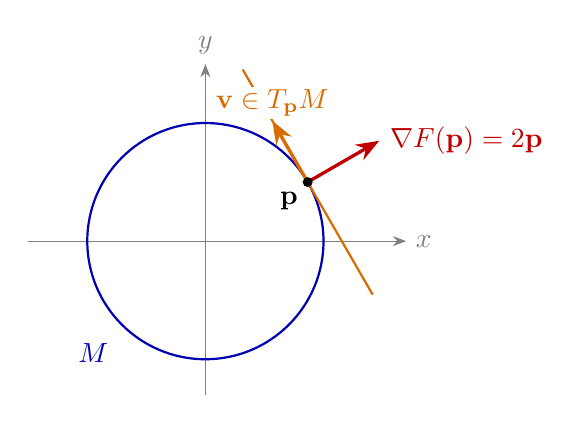
\begin{tikzpicture}[scale=1.5, >=Stealth]
        \draw[->, gray] (-1.5,0) -- (1.7,0) node[right] {$x$};
        \draw[->, gray] (0,-1.3) -- (0,1.5) node[above] {$y$};
        \draw[blue!70!black, thick] (0,0) circle (1);
        \coordinate (P) at (30:1);
        \draw[orange!85!black, thick] ($(P) + (120:1.1)$) -- ($(P) + (-60:1.1)$);
        \draw[->, very thick, red!75!black] (P) -- ($(P) + (30:0.7)$) node[right] {$\nabla F(\mathbf{p}) = 2\mathbf{p}$};
        \draw[->, very thick, orange!85!black] (P) -- ($(P) + (120:0.6)$) node[above, fill=white, inner sep=1pt] {$\mathbf{v} \in T_{\mathbf{p}}M$};
        \fill (P) circle (1.2pt) node[below left] {$\mathbf{p}$};
        \node[blue!70!black] at (-0.95,-0.95) {$M$};
    \end{tikzpicture}
    \caption{The circle $M = \{F = 0\}$ with $F(x, y) = x^2 + y^2 - 1$. The tangent space $T_{\mathbf{p}}M = \Null DF(\mathbf{p}) = \mathbf{p}^\perp$ is the tangent line (shifted to $\mathbf{p}$), and the normal space is spanned by the gradient $\nabla F(\mathbf{p})$.}
    \label{A-fig:tangent}
\end{figure}

\begin{example}\label{A-ex:tangent-spaces}
    \begin{enumerate}
        \item $T_{\mathbf{p}}S^{n-1} = \Null(2\mathbf{p}^\top) = \{\mathbf{v} : \mathbf{p}^\top\mathbf{v} = 0\} = \mathbf{p}^\perp$: the tangent vectors of a sphere are orthogonal to the radius (Figure~\ref{A-fig:tangent}).
        \item $T_I SL(n, \mathbb{R}) = \{H : D\det(I)H = 0\} = \{H : \tr H = 0\}$, the traceless matrices: to first order, $\det(I + tH) = 1 + t\tr H$ (Lemma~\ref{L3-lem:det-identity}), so a matrix curve through $I$ keeps determinant $1$ only if its velocity has trace $0$.
        \item $T_Q O(n) = \{H : H^\top Q + Q^\top H = 0\}$. With $K = Q^\top H$, the condition says $K^\top + K = 0$, so $T_Q O(n) = \{QK : K^\top = -K\}$, and $T_I O(n)$ is the space of skew-symmetric matrices, of dimension $\frac{n(n-1)}{2}$. For example, the rotations $R(t)$ by the angle $t$ in the plane have $R'(0) = \begin{pmatrix} 0 & -1 \\ 1 & 0 \end{pmatrix}$.
    \end{enumerate}
\end{example}

\section{Lagrange Multipliers and Optimization on Manifolds}\label{A-sec:lagrange}

We can now complete the proof of the Lagrange multiplier theorem (Theorem~\ref{L3-thm:lagrange}).

\begin{theorem}[Lagrange multipliers]\label{A-thm:lagrange-proof}
    Let $f$ and $g_1, \ldots, g_m$ be smooth on an open set $U \subseteq \mathbb{R}^n$, let $\mathbf{x}^*$ be a local minimum of $f$ on $M = \{\mathbf{x} \in U : g_1(\mathbf{x}) = \cdots = g_m(\mathbf{x}) = 0\}$, and let $\nabla g_1(\mathbf{x}^*), \ldots, \nabla g_m(\mathbf{x}^*)$ be linearly independent. Then $\nabla f(\mathbf{x}^*) \in \Span\{\nabla g_1(\mathbf{x}^*), \ldots, \nabla g_m(\mathbf{x}^*)\}$, i.e., there are $\lambda_i$ with $\nabla f(\mathbf{x}^*) + \sum_i \lambda_i\nabla g_i(\mathbf{x}^*) = \mathbf{0}$.
\end{theorem}

\begin{proof}
    The linear independence says that $DG(\mathbf{x}^*)$ has rank $m$ for $G = (g_1, \ldots, g_m)$, so near $\mathbf{x}^*$, $M$ is an $(n - m)$-dimensional submanifold (the rank stays $m$ near $\mathbf{x}^*$, since a nonzero $m \times m$ minor stays nonzero by continuity). For every $\mathbf{v} \in T_{\mathbf{x}^*}M$, choose a curve $\boldsymbol{\gamma}$ in $M$ with $\boldsymbol{\gamma}(0) = \mathbf{x}^*$ and $\boldsymbol{\gamma}'(0) = \mathbf{v}$. The function $t \mapsto f(\boldsymbol{\gamma}(t))$ has a local minimum at $t = 0$, so its derivative $\nabla f(\mathbf{x}^*)^\top\mathbf{v}$ is $0$. Hence $\nabla f(\mathbf{x}^*) \in (T_{\mathbf{x}^*}M)^\perp = N_{\mathbf{x}^*}M = \Span\{\nabla g_i(\mathbf{x}^*)\}$ by Theorem~\ref{A-thm:tangent-space}.
\end{proof}

The proof suggests how to do calculus on a manifold: only the component of $\nabla f$ in the tangent space matters.

\begin{definition}[Riemannian gradient]\label{A-def:riemannian-gradient}
    Let $M$ be a submanifold of $\mathbb{R}^n$, $\mathbf{p} \in M$, and $f$ smooth near $M$. The Riemannian gradient of $f$ on $M$ at $\mathbf{p}$ is the orthogonal projection (Lecture~2) of $\nabla f(\mathbf{p})$ onto $T_{\mathbf{p}}M$:
    \[\grad_M f(\mathbf{p}) = P_{\mathbf{p}}\nabla f(\mathbf{p}).\]
\end{definition}

Since $\nabla f(\mathbf{p}) - \grad_M f(\mathbf{p})$ is orthogonal to $T_{\mathbf{p}}M$, we have $\nabla f(\mathbf{p})^\top\mathbf{v} = \grad_M f(\mathbf{p})^\top\mathbf{v}$ for all tangent vectors $\mathbf{v}$: the Riemannian gradient gives the rates of change of $f$ along $M$. As in Theorem~\ref{L3-thm:steepest}, it points in the direction of steepest ascent among the tangent directions, and by Theorem~\ref{A-thm:lagrange-proof}, $\grad_M f(\mathbf{p}) = \mathbf{0}$ exactly at the points that satisfy the Lagrange condition. These points are the critical points of $f$ on $M$.

Riemannian gradient descent minimizes $f$ on $M$ by taking a step in the direction $-\grad_M f(\mathbf{p}_k)$, which leaves $M$ slightly, and mapping the result back to $M$ with a retraction $R$:
\[\mathbf{p}_{k+1} = R\big(\mathbf{p}_k - \eta\grad_M f(\mathbf{p}_k)\big).\]
On the sphere, $P_{\mathbf{p}} = I - \mathbf{p}\mathbf{p}^\top$, so $\grad_M f(\mathbf{p}) = \nabla f(\mathbf{p}) - (\mathbf{p}^\top\nabla f(\mathbf{p}))\mathbf{p}$, and the retraction can simply normalize: $R(\mathbf{x}) = \frac{\mathbf{x}}{\norm{\mathbf{x}}}$. On $O(n)$, one can retract with the $Q$ factor of the QR decomposition (Lecture~2). Such methods are used for PCA, for orthogonality constraints on weight matrices, and for low-rank matrix problems.

\begin{example}[The Rayleigh quotient on the sphere]\label{A-ex:rayleigh-sphere}
    Let $A$ be symmetric with eigenvalues $\lambda_1 > \lambda_2 > \cdots > \lambda_n$ and unit eigenvectors $\mathbf{q}_1, \ldots, \mathbf{q}_n$, and let $f(\mathbf{x}) = \mathbf{x}^\top A\mathbf{x}$ on $S^{n-1}$. Then $\grad_M f(\mathbf{x}) = 2A\mathbf{x} - 2(\mathbf{x}^\top A\mathbf{x})\mathbf{x}$, which is $\mathbf{0}$ if and only if $\mathbf{x}$ is an eigenvector: the critical points are the $2n$ points $\pm\mathbf{q}_i$. To see their types, move from $\mathbf{q}_i$ towards $\mathbf{q}_j$ along the great circle $\boldsymbol{\gamma}(t) = \cos t\,\mathbf{q}_i + \sin t\,\mathbf{q}_j$:
    \[f(\boldsymbol{\gamma}(t)) = \lambda_i\cos^2 t + \lambda_j\sin^2 t = \lambda_i + (\lambda_j - \lambda_i)\sin^2 t.\]
    So $f$ decreases in the $n - i$ tangent directions $\mathbf{q}_j$ with $\lambda_j < \lambda_i$, and increases in the $i - 1$ directions with $\lambda_j > \lambda_i$. Hence $\pm\mathbf{q}_1$ are the maxima, $\pm\mathbf{q}_n$ the minima, and all other eigenvectors are saddle points. In particular, Riemannian gradient ascent for the first principal component (Lecture~2) has exactly one pair of local maxima, the correct answer; the other critical points are saddle points, which gradient ascent avoids from almost every starting point.
\end{example}

\section{Critical Points and Morse Theory}\label{A-sec:morse}

\subsection{Regular and critical values}

\begin{definition}[Critical points and values of maps]\label{A-def:critical-maps}
    Let $F: U \to \mathbb{R}^m$ be smooth on an open set $U \subseteq \mathbb{R}^n$. A point $\mathbf{x}$ is a critical point of $F$ if $\rank DF(\mathbf{x}) < m$, and a value $\mathbf{c}$ is a critical value if $\mathbf{c} = F(\mathbf{x})$ for a critical point $\mathbf{x}$. All other values in $\mathbb{R}^m$ are regular values.
\end{definition}

For $m = 1$, the critical points are the points with $\nabla F(\mathbf{x}) = \mathbf{0}$, as in Lecture~3. By Section~\ref{A-sec:manifolds}, the level set of a regular value is a submanifold (or empty). How many critical values can there be? A set $Z \subseteq \mathbb{R}^m$ has measure zero if for every $\varepsilon > 0$ it can be covered by countably many boxes whose volumes add up to less than $\varepsilon$. For example, finite and countable sets, and lines in $\mathbb{R}^2$, have measure zero.

\begin{theorem}[Sard]\label{A-thm:sard}
    The set of critical values of a smooth map $F: U \to \mathbb{R}^m$ has measure zero.
\end{theorem}

We do not prove this theorem. It says that almost every value is regular, so almost every level set of a smooth function $f: U \to \mathbb{R}$ is an $(n - 1)$-dimensional submanifold or empty. Note that the theorem is about values, not points: a constant function has only critical points, but only one critical value.

\subsection{Nondegenerate critical points}

From now on, let $f: U \to \mathbb{R}$ be smooth. Lecture~3 classified critical points by the eigenvalues of the Hessian (Theorem~\ref{L3-thm:second-order}). The test was inconclusive when an eigenvalue is $0$.

\begin{definition}[Nondegenerate critical points and the index]\label{A-def:index}
    A critical point $\mathbf{p}$ of $f$ is nondegenerate if the Hessian $\nabla^2 f(\mathbf{p})$ is invertible, i.e., has no eigenvalue $0$. Its index is the number of negative eigenvalues of $\nabla^2 f(\mathbf{p})$, counted with multiplicity. A function whose critical points are all nondegenerate is a Morse function.
\end{definition}

So a nondegenerate critical point of index $0$ is a strict local minimum, one of index $n$ is a strict local maximum, and all others are saddle points. The index counts the independent directions in which $f$ decreases. For example, $x^3 + y^3 - 3xy$ (Example~\ref{L3-ex:critical-points}) is a Morse function, with a critical point of index $1$ at the origin and one of index $0$ at $(1, 1)$. The ``monkey saddle'' $x^3 - 3xy^2$ has a degenerate critical point at the origin, where its Hessian is $0$; near the origin, it goes up and down three times, unlike any nondegenerate saddle.

\begin{proposition}\label{A-prop:isolated}
    Nondegenerate critical points are isolated: each one has a neighborhood that contains no other critical point.
\end{proposition}

\begin{proof}
    Let $H = \nabla^2 f(\mathbf{p})$, and let $\mu > 0$ be the smallest absolute value of an eigenvalue of $H$. Writing $\mathbf{h}$ in an orthonormal eigenbasis (Lecture~2) shows $\norm{H\mathbf{h}} \geq \mu\norm{\mathbf{h}}$. The gradient is differentiable with derivative $H$ at $\mathbf{p}$, so $\nabla f(\mathbf{p} + \mathbf{h}) = H\mathbf{h} + \mathbf{r}(\mathbf{h})$ with $\norm{\mathbf{r}(\mathbf{h})} \leq \frac{\mu}{2}\norm{\mathbf{h}}$ for small $\mathbf{h}$. Then $\norm{\nabla f(\mathbf{p} + \mathbf{h})} \geq \frac{\mu}{2}\norm{\mathbf{h}} > 0$ for small $\mathbf{h} \neq \mathbf{0}$.
\end{proof}

In Lecture~3, we saw that near a critical point, $f$ is approximately a sum of parabolas, $f(\mathbf{p}) + \frac{1}{2}\sum_i \lambda_i y_i^2$, in the coordinates given by the eigenvectors of the Hessian. For nondegenerate critical points, this becomes exact after a nonlinear change of coordinates.

\begin{theorem}[Morse lemma]\label{A-thm:morse-lemma}
    Let $\mathbf{p}$ be a nondegenerate critical point of $f$ with index $k$. Then there is a diffeomorphism $\boldsymbol{\varphi}$ from a neighborhood of $\mathbf{p}$ onto a neighborhood of $\mathbf{0}$, with $\boldsymbol{\varphi}(\mathbf{p}) = \mathbf{0}$, such that in the coordinates $\mathbf{y} = \boldsymbol{\varphi}(\mathbf{x})$,
    \[f = f(\mathbf{p}) - y_1^2 - \cdots - y_k^2 + y_{k+1}^2 + \cdots + y_n^2.\]
\end{theorem}

We do not prove the Morse lemma. It says that near a nondegenerate critical point, the higher-order terms of the Taylor expansion do not change the picture at all: up to a smooth deformation, the function is a bowl, a saddle with $k$ downward directions, or an upside-down bowl. Degenerate critical points can be much more complicated, but they are rare.

\begin{theorem}[Morse functions are generic]\label{A-thm:morse-generic}
    Let $f: U \to \mathbb{R}$ be smooth. For almost every $\mathbf{a} \in \mathbb{R}^n$ (all except a set of measure zero), the function $f_{\mathbf{a}}(\mathbf{x}) = f(\mathbf{x}) - \mathbf{a}^\top\mathbf{x}$ is a Morse function.
\end{theorem}

\begin{proof}
    We have $\nabla f_{\mathbf{a}} = \nabla f - \mathbf{a}$ and $\nabla^2 f_{\mathbf{a}} = \nabla^2 f$. So $\mathbf{x}$ is a critical point of $f_{\mathbf{a}}$ if and only if $\nabla f(\mathbf{x}) = \mathbf{a}$, and it is degenerate if and only if $\nabla^2 f(\mathbf{x})$, the Jacobian of the map $\nabla f: U \to \mathbb{R}^n$, is singular. Hence $f_{\mathbf{a}}$ has a degenerate critical point if and only if $\mathbf{a}$ is a critical value of $\nabla f$, and by Sard's theorem, these $\mathbf{a}$ form a set of measure zero.
\end{proof}

For example, $f(x) = x^3$ has a degenerate critical point at $0$, but $x^3 - ax$ is a Morse function for every $a \neq 0$: it has two nondegenerate critical points if $a > 0$, and none if $a < 0$. An arbitrarily small, random linear perturbation removes all degenerate critical points.

\subsection{Critical points and the shape of sublevel sets}

Morse theory studies how the sublevel sets $M^c = \{\mathbf{x} : f(\mathbf{x}) \leq c\}$ change as $c$ increases. We state its two main results informally, for a Morse function $f$ whose sublevel sets are compact (for example, a Morse function on a compact manifold, or a coercive Morse function on $\mathbb{R}^n$).
\begin{itemize}
    \item If there are no critical values in $[a, b]$, then $M^a$ and $M^b$ have the same shape: $M^b$ can be continuously deformed into $M^a$, by flowing downhill along $-\nabla f$. Nothing interesting happens between critical values.
    \item When $c$ passes the value of a critical point of index $k$, the sublevel set changes by attaching a $k$-dimensional ``cell'' (a point for $k = 0$, a segment for $k = 1$, a disk for $k = 2$, and so on). A minimum ($k = 0$) creates a new connected component. A saddle point of index $1$ attaches a bridge, which either connects two components or closes a loop.
\end{itemize}

\begin{example}[A double well]\label{A-ex:double-well}
    The function $f(x, y) = (x^2 - 1)^2 + y^2$ has $\nabla f = (4x(x^2 - 1), 2y)$, so its critical points are $(\pm 1, 0)$, with $f = 0$ and $\nabla^2 f = \diag(8, 2)$ (index $0$), and $(0, 0)$, with $f = 1$ and $\nabla^2 f = \diag(-4, 2)$ (index $1$). For $c < 0$, the sublevel set is empty; at $c = 0$, two components appear at the minima; at $c = 1$, the saddle point attaches a bridge that joins them, and for $c > 1$, the sublevel set is connected (Figure~\ref{A-fig:double-well}). For gradient descent, this means that the two basins of the minima are separated by the saddle: an iteration that starts with $f(\mathbf{x}_0) < 1$ and decreases $f$ in every step cannot move from one basin to the other.
\end{example}

\begin{figure}[ht]
    \centering
    \foreach \c/\lab in {0.5/{c = 0.5}, 1/{c = 1}, 1.8/{c = 1.8}} {
        \begin{tikzpicture}[scale=1.15, >=Stealth]
            \pgfmathsetmacro{\s}{sqrt(\c)}
            \ifdim \c pt < 1.01pt
                \foreach \sgn in {1,-1}
                    \filldraw[fill=blue!15, draw=blue!70!black, thick, domain=-180:180, samples=120, variable=\t, smooth]
                        plot ({\sgn*sqrt(max(0, 1 + \s*cos(\t)))}, {\s*sin(\t)}) -- cycle;
            \else
                \pgfmathsetmacro{\tz}{acos(-1/\s)}
                \filldraw[fill=blue!15, draw=blue!70!black, thick, smooth]
                    plot[domain=-\tz:\tz, samples=90, variable=\t] ({sqrt(max(0, 1 + \s*cos(\t)))}, {\s*sin(\t)})
                    -- plot[domain=\tz:-\tz, samples=90, variable=\t] ({-sqrt(max(0, 1 + \s*cos(\t)))}, {\s*sin(\t)}) -- cycle;
            \fi
            \draw[->, gray] (-1.75,0) -- (1.85,0) node[right] {$x$};
            \draw[->, gray] (0,-1.45) -- (0,1.55) node[above] {$y$};
            \fill (1,0) circle (1.3pt);
            \fill (-1,0) circle (1.3pt);
            \fill[red!75!black] (0,0) circle (1.3pt);
            \node at (0,-1.75) {$\lab$};
        \end{tikzpicture}\hspace{0.6em}
    }
    \caption{Sublevel sets $\{f \leq c\}$ of the double well $f(x, y) = (x^2 - 1)^2 + y^2$, with the two minima (black, index $0$, value $0$) and the saddle point (red, index $1$, value $1$). Below the critical value $1$, the sublevel set has two components; at $c = 1$, they touch at the saddle point; above it, they have merged into one.}
    \label{A-fig:double-well}
\end{figure}

On a compact manifold, these changes must add up. The Euler characteristic $\chi(M)$ is a number that only depends on the topology of $M$: for a surface divided into $V$ vertices, $E$ edges and $F$ faces, it is $V - E + F$, which does not depend on the subdivision. For example, the sphere has $\chi = 2$ (a cube has $8 - 12 + 6 = 2$), and the torus (the surface of a doughnut) has $\chi = 0$.

\begin{theorem}[Morse relation]\label{A-thm:morse-relation}
    Let $f$ be a Morse function on a compact manifold $M$, and let $c_k$ be the number of its critical points of index $k$. Then
    \[\chi(M) = c_0 - c_1 + c_2 - \cdots + (-1)^n c_n.\]
\end{theorem}

We do not prove this theorem; it follows from the fact that attaching a $k$-cell changes the Euler characteristic by $(-1)^k$. It shows that the topology of $M$ forces critical points to exist, whatever function we choose.

\begin{example}\label{A-ex:morse-relation}
    \begin{enumerate}
        \item The height function on the sphere $S^2$ has a minimum and a maximum: $\chi(S^2) = 1 - 0 + 1 = 2$.
        \item The height function on an upright torus has a minimum, two saddle points and a maximum (Figure~\ref{A-fig:torus}): $\chi = 1 - 2 + 1 = 0$. In fact, every Morse function on the torus has at least four critical points, at least two of which are saddle points (this follows from the Morse inequalities, which we do not discuss).
        \item For the Rayleigh quotient on $S^{n-1}$ (Example~\ref{A-ex:rayleigh-sphere}), the two critical points $\pm\mathbf{q}_i$ have index $n - i$, so $\sum_k (-1)^k c_k = 2\sum_{i=1}^n (-1)^{n-i}$, which is $2$ for odd $n$ and $0$ for even $n$. This agrees with the Euler characteristic of the sphere $S^{n-1}$, which is $2$ if $n - 1$ is even and $0$ if $n - 1$ is odd. For $n = 3$ and $A = \diag(3, 2, 1)$: two maxima $\pm\mathbf{e}_1$, two saddle points $\pm\mathbf{e}_2$, two minima $\pm\mathbf{e}_3$, and $2 - 2 + 2 = 2$.
    \end{enumerate}
\end{example}

\begin{figure}[ht]
    \centering
    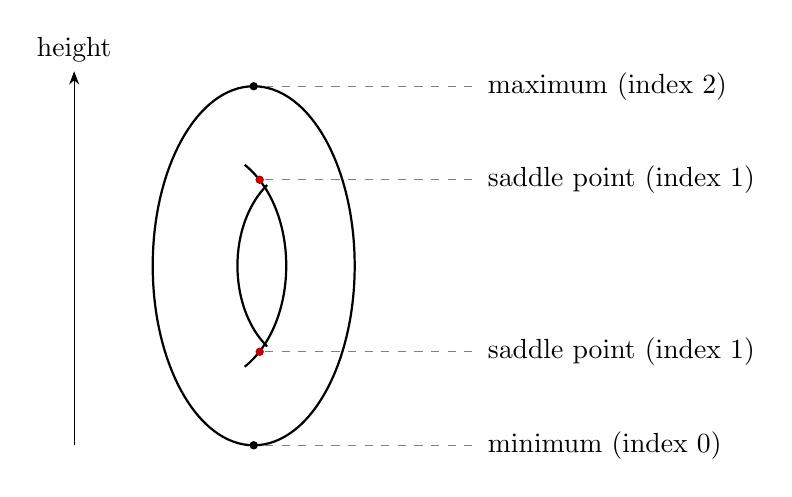
\begin{tikzpicture}[scale=0.95, >=Stealth]
        \begin{scope}[rotate=90]
            \draw[thick] (0,0) ellipse (2.4 and 1.35);
            \draw[thick] (-1.35,0.12) .. controls (-0.75,-0.62) and (0.75,-0.62) .. (1.35,0.12);
            \draw[thick] (-1.08,-0.18) .. controls (-0.55,0.35) and (0.55,0.35) .. (1.08,-0.18);
            \fill (-2.4,0) circle (1.6pt);
            \fill[red!75!black] (-1.15,-0.08) circle (1.6pt);
            \fill[red!75!black] (1.15,-0.08) circle (1.6pt);
            \fill (2.4,0) circle (1.6pt);
        \end{scope}
        \draw[dashed, gray] (0.15,-2.4) -- (3.0,-2.4) node[right, black] {minimum (index $0$)};
        \draw[dashed, gray] (0.15,-1.15) -- (3.0,-1.15) node[right, black] {saddle point (index $1$)};
        \draw[dashed, gray] (0.15,1.15) -- (3.0,1.15) node[right, black] {saddle point (index $1$)};
        \draw[dashed, gray] (0.15,2.4) -- (3.0,2.4) node[right, black] {maximum (index $2$)};
        \draw[->] (-2.4,-2.4) -- (-2.4,2.6) node[above] {height};
    \end{tikzpicture}
    \caption{The height function on an upright torus has four critical points: the bottom (a minimum), the bottom and the top of the hole (two saddle points), and the top (a maximum). As the height $c$ increases, the sublevel set is first a disk around the bottom (after the minimum), then a bent tube, i.e., a cylinder (after the first saddle point, where the disk closes up around the tube), then a torus with a hole at its top (after the second saddle point, where the two ends of the tube meet and close a loop around the hole of the torus), and finally the whole torus (after the maximum).}
    \label{A-fig:torus}
\end{figure}

\section{Topology in Machine Learning}\label{A-sec:ml}

We end with a few places where the ideas of this appendix appear in machine learning. Some of them are theorems, others are well-supported heuristics and active research topics.
\begin{itemize}
    \item \textbf{The manifold hypothesis.} High-dimensional data, such as images with millions of pixels, are believed to lie close to submanifolds of much smaller dimension: the images of a face, for example, vary with a small number of parameters such as pose, lighting and expression. PCA finds the best approximating linear subspace (Lecture~2); autoencoders and other nonlinear methods try to find curved, manifold-like structures.
    \item \textbf{Normalizing flows and topology.} A normalizing flow maps a simple distribution, such as a Gaussian on $\mathbb{R}^n$, to a complicated one by a diffeomorphism (Corollary~\ref{A-cor:residual} and Remark~\ref{L3-rem:change-of-variables}). Diffeomorphisms preserve topology. So, by Proposition~\ref{A-prop:connected}, a flow cannot map $\mathbb{R}^n$, which is connected, exactly onto a distribution supported on two separate pieces, such as two clusters: it can only approximate it by squeezing a little probability mass through thin bridges between them.
    \item \textbf{Symmetries make critical points degenerate.} If a loss is invariant under a continuous family of transformations of the parameters, its minima are not isolated. For example, the ReLU satisfies $\max(0, ct) = c\max(0, t)$ for $c > 0$, so multiplying the incoming weights of a hidden unit by $c$ and its outgoing weights by $\frac{1}{c}$ does not change the network. The set of minima then contains curves (in the simplest case, the hyperbola $w_1 w_2 = 1$ for the loss $(w_1 w_2 - 1)^2$), and by Proposition~\ref{A-prop:isolated}, the Hessian at a minimum must have the eigenvalue $0$, in the tangent directions of these curves. Loss functions of neural networks are therefore not Morse functions.
    \item \textbf{Saddle points in high dimensions.} At a critical point of a loss with millions of parameters, all eigenvalues of the Hessian must be nonnegative for a local minimum. A heuristic, supported by experiments and by random matrix theory, says that critical points with high loss usually have many negative eigenvalues, i.e., a large index: they are saddle points rather than bad local minima. Gradient descent with noise, as in SGD, tends to escape from saddle points, which is part of the explanation why training works.
    \item \textbf{Connected sublevel sets.} Experiments show that two minima found by training the same network twice can often be joined by a path along which the loss stays low (``mode connectivity''): the sublevel sets $\{L \leq c\}$ for small $c$ seem to be connected, up to the symmetries of the network. Morse theory gives a language for such statements: a sublevel set can only become connected by passing saddle points of index $1$.
\end{itemize}

\section*{Key Takeaways}
\addcontentsline{toc}{section}{Key Takeaways}
\begin{itemize}[leftmargin=*]
    \item Open sets, closed sets, convergence and continuity only depend on the notion of nearness. A map is continuous if and only if preimages of open sets are open; so sublevel sets $\{f \leq c\}$ and level sets of continuous functions are closed. All norms on $\mathbb{R}^n$ define the same open sets.
    \item A subset of $\mathbb{R}^n$ is compact if and only if it is closed and bounded (Heine--Borel). A continuous function on a nonempty compact set attains its minimum and maximum, and a continuous coercive function on $\mathbb{R}^n$ has a global minimum; regularization makes losses coercive.
    \item Continuous maps preserve connectedness; this gives the intermediate value theorem, and shows, e.g., that $GL(n, \mathbb{R})$ has two pieces and that a circle is not homeomorphic to an interval.
    \item A contraction of a closed set has a unique fixed point, found by iteration (Banach). This proves the inverse function theorem: a map with an invertible Jacobian is locally invertible, with $D(\mathbf{f}^{-1}) = (D\mathbf{f})^{-1}$. Residual layers $\mathbf{x} + \mathbf{g}(\mathbf{x})$ with a contractive $\mathbf{g}$ are invertible.
    \item The implicit function theorem solves $F(\mathbf{x}, \mathbf{y}) = \mathbf{0}$ locally for $\mathbf{y} = \mathbf{g}(\mathbf{x})$ when $D_{\mathbf{y}}F$ is invertible, with $D\mathbf{g} = -D_{\mathbf{y}}F^{-1}D_{\mathbf{x}}F$; this is implicit differentiation, also used for implicit layers and hyperparameter optimization.
    \item The level set of a regular value of $F: \mathbb{R}^n \to \mathbb{R}^m$ is an $(n - m)$-dimensional submanifold, which is locally a graph. Its tangent space is $\Null DF(\mathbf{p})$, and its normal space is spanned by the gradients $\nabla F_i(\mathbf{p})$. Examples: spheres, $SL(n)$ (dimension $n^2 - 1$, tangent space at $I$: traceless matrices), $O(n)$ (dimension $\frac{n(n-1)}{2}$, tangent space at $I$: skew-symmetric matrices).
    \item Lagrange multipliers say that $\nabla f$ is normal to the constraint manifold at a constrained extremum. The Riemannian gradient is the projection of $\nabla f$ onto the tangent space; Riemannian gradient descent alternates such steps with retractions.
    \item By Sard's theorem, almost all values of a smooth map are regular. A critical point is nondegenerate if its Hessian is invertible, and its index is the number of negative eigenvalues. Nondegenerate critical points are isolated, and by the Morse lemma $f$ is exactly a sum of $\pm y_i^2$ near them. Almost every linear perturbation of a function is a Morse function.
    \item Sublevel sets change their topology only at critical values: a critical point of index $k$ attaches a $k$-cell. On a compact manifold, $\chi(M) = \sum_k (-1)^k c_k$.
\end{itemize}

\section*{Exercises}
\addcontentsline{toc}{section}{Exercises}
\begin{enumerate}[leftmargin=*]
    \item Which of the following subsets of $\mathbb{R}^2$ are open, closed, both or neither? Find their interior, closure and boundary: (a) $\{x > 0, y > 0\}$; (b) $\{x^2 + y^2 \leq 1\}$; (c) $\{(x, 0) : 0 \leq x < 1\}$; (d) $\mathbb{Q}^2$, the points with rational coordinates.
    \item Show that the union of infinitely many closed sets need not be closed. Show that a set $U \subseteq X$ is open if and only if it is a union of open balls.
    \item \begin{enumerate}[label=(\alph*)]
        \item Show that the set of $m \times n$ matrices of rank at most $r$ is closed in $\mathbb{R}^{m \times n}$. (Hint: the rank is at most $r$ if and only if all $(r + 1) \times (r + 1)$ minors are $0$.)
        \item Show that every square matrix $A$ is a limit of invertible matrices. (Hint: $\det(A + tI)$ is a polynomial in $t$.) So $GL(n, \mathbb{R})$ is open and dense in $\mathbb{R}^{n \times n}$.
    \end{enumerate}
    \item Which of the following sets are compact? (a) The closed unit ball of the $\ell_1$ norm in $\mathbb{R}^n$; (b) $\{(x, y) : xy = 1\}$; (c) $SO(n)$; (d) $GL(n, \mathbb{R})$; (e) the ellipsoid $\{\mathbf{x} : \mathbf{x}^\top A\mathbf{x} \leq 1\}$ for a symmetric positive definite $A$; (f) the same set for $A = \diag(1, -1)$.
    \item Show that the regularized logistic regression loss $\frac{1}{N}\sum_i \log(1 + e^{-y_i\mathbf{w}^\top\mathbf{x}_i}) + \lambda\norm{\mathbf{w}}^2$ with $\lambda > 0$ has a global minimum, and that it is unique. (Use Proposition~\ref{A-prop:coercive} and Lecture~3.)
    \item Let $A \in \mathbb{R}^{n \times n}$. Show that $N(\mathbf{x}) = \norm{A\mathbf{x}}$ is a norm if and only if $A$ is invertible, and that the best constants in $c\norm{\mathbf{x}} \leq N(\mathbf{x}) \leq C\norm{\mathbf{x}}$ are the smallest and the largest singular value of $A$ (Lecture~2).
    \item \begin{enumerate}[label=(\alph*)]
        \item Show that the unit circle $S^1$ is path-connected, and that the hyperbola $\{x^2 - y^2 = 1\}$ is not connected.
        \item Show that $SO(2)$ is path-connected, and that $O(2)$ is not connected.
        \item Show that no continuous injective map from $S^1$ to $\mathbb{R}$ exists. (Hint: intermediate value theorem.)
    \end{enumerate}
    \item Use the iteration $x_{k+1} = \cos x_k$ with $x_0 = 1$ to compute the solution of $\cos x = x$ to six decimal places. How many steps does the a priori bound of Theorem~\ref{A-thm:banach} require, and how many do you actually need?
    \item Show that $f(x) = x + \frac{1}{2}\tanh(x)$ is a homeomorphism of $\mathbb{R}$, and compute $f^{-1}(1)$ with the iteration of Corollary~\ref{A-cor:residual}, starting at $x_0 = 0$. Is $f$ a diffeomorphism?
    \item At which points of the folium $x^3 + y^3 = 3xy$ can the curve not be written locally as a graph $y = g(x)$? Compute $g'(x)$ at the point $(\frac{3}{2}, \frac{3}{2})$.
    \item Let $F(x, y, z) = x^2 + y^2 - z^2$. Find all critical points and critical values of $F$. For which $c$ is $F^{-1}(c)$ a submanifold? Describe the level sets for $c > 0$, $c = 0$ and $c < 0$; which of them are connected?
    \item \begin{enumerate}[label=(\alph*)]
        \item Find the tangent space of the sphere $x^2 + y^2 + z^2 = 9$ at $(1, 2, 2)$ as $\Null DF$, and the tangent plane $(1, 2, 2) + T_{(1, 2, 2)}M$ as an equation.
        \item Show that $T_Q O(n) = \{QK : K^\top = -K\}$ and $T_I SL(n, \mathbb{R}) = \{H : \tr H = 0\}$ have the dimensions predicted by Example~\ref{A-ex:submanifolds}.
    \end{enumerate}
    \item (Orthogonal Procrustes problem.) Given $A \in \mathbb{R}^{n \times n}$ with SVD $A = U\Sigma V^\top$, show that $\tr(Q^\top A)$ is maximal over $Q \in O(n)$ for $Q = UV^\top$. (Hint: $\tr(Q^\top A) = \tr(\Sigma Z)$ with the orthogonal matrix $Z = V^\top Q^\top U$, whose entries are at most $1$ in absolute value.) This is how one aligns two point clouds by a rotation or reflection.
    \item \begin{enumerate}[label=(\alph*)]
        \item Find all critical points of the monkey saddle $f(x, y) = x^3 - 3xy^2$. Show that the origin is a degenerate critical point. In polar coordinates, $f = r^3\cos 3\varphi$; describe the regions where $f > 0$ and $f < 0$.
        \item For which $a \in \mathbb{R}$ is $x^3 - ax$ a Morse function? Find its critical points and their indices.
        \item Find the critical points and their indices of $f(x, y) = x^4 - 2x^2 + y^2 + \varepsilon x$ for a small $\varepsilon > 0$, and describe how the sublevel sets change as $c$ increases.
    \end{enumerate}
    \item Let $A = \diag(3, 2, 1)$ and $f(\mathbf{x}) = \mathbf{x}^\top A\mathbf{x}$ on the sphere $S^2$. Find all critical points of $f$ and their indices, and check the Morse relation $\chi(S^2) = 2$. Repeat for $A = \diag(4, 3, 2, 1)$ on $S^3$, whose Euler characteristic is $0$.
\end{enumerate}

\section*{Programming Exercises}
\addcontentsline{toc}{section}{Programming Exercises}

% Inline code cannot be hyphenated, so allow a little extra stretch in this section.
\setlength{\emergencystretch}{3em}

As in Lecture~3, use NumPy (and Matplotlib for plots), and start each file with
\begin{lstlisting}
import numpy as np
import matplotlib.pyplot as plt
rng = np.random.default_rng(0)
\end{lstlisting}

\begin{enumerate}[label=\textbf{P\arabic*.}, leftmargin=*]
    \item \textbf{Inverting a residual layer.} Let \py{W = rng.normal(size=(5, 5))} and $\mathbf{g}(\mathbf{x}) = c\tanh(W\mathbf{x})$ with $c = 0.9/\norm{W}_2$.
    \begin{itemize}
        \item Show that $\mathbf{g}$ is Lipschitz continuous with constant $0.9$ (use $|\tanh'| \leq 1$ and Lemma~\ref{A-lem:mean-value}).
        \item For a random $\mathbf{x}$, compute $\mathbf{y} = \mathbf{x} + \mathbf{g}(\mathbf{x})$, and recover $\mathbf{x}$ with the iteration of Corollary~\ref{A-cor:residual}. Plot the error against the number of iterations on a logarithmic scale, together with the bound of Theorem~\ref{A-thm:banach}.
        \item Repeat with $c = 1.5/\norm{W}_2$. Does the iteration still converge? Is $\mathbf{x} \mapsto \mathbf{x} + \mathbf{g}(\mathbf{x})$ still injective? (Try to find two points with the same image.)
    \end{itemize}

    \item \textbf{Riemannian gradient ascent on the sphere.} For a random symmetric $A = B + B^\top$ with \py{B = rng.normal(size=(6, 6))}, maximize $f(\mathbf{x}) = \mathbf{x}^\top A\mathbf{x}$ on $S^5$ with the Riemannian gradient and the normalization retraction (Section~\ref{A-sec:lagrange}).
    \begin{itemize}
        \item Start from $100$ random points, and check that you always reach $\pm\mathbf{q}_1$ (compare with \py{np.linalg.eigh}). Plot $f(\mathbf{p}_k)$ for a few runs.
        \item Start exactly at an eigenvector $\mathbf{q}_i$ with $i > 1$. What happens? Now add a perturbation of size $10^{-8}$. How many steps does it take to escape from the saddle point, and how does this depend on $\lambda_1 - \lambda_i$?
    \end{itemize}

    \item \textbf{Orthogonal Procrustes.} Generate a point cloud \py{X = rng.normal(size=(50, 3))}, a random orthogonal matrix $Q_0$ (from \py{np.linalg.qr}), and $Y = XQ_0^\top + 0.01\cdot$noise. Recover $Q_0$ by maximizing $\tr(Q^\top Y^\top X)$ over $O(3)$ with the SVD formula of Exercise~13. Then solve the same problem with Riemannian gradient ascent on $O(3)$: project $G = \nabla_Q$ onto $T_Q O(3)$ by $Q\,\frac{1}{2}(Q^\top G - G^\top Q)$, take a step, and retract with the $Q$ factor of a QR decomposition (fixing the signs so that the diagonal of $R$ is positive). Compare the results.

    \item \textbf{Counting components of sublevel sets.} For $f(x, y) = x^4 - 2x^2 + y^2 + 0.3x$, evaluate $f$ on a fine grid over $[-2, 2]^2$, and for $50$ values of $c$, count the connected components of the grid points with $f \leq c$ (write a breadth-first search over neighboring grid points). Plot the number of components against $c$, and compare the values of $c$ where it changes with the critical values of $f$, which you can find with Newton's method applied to $\nabla f = \mathbf{0}$.
\end{enumerate}
\endgroup

% Generated by make_book.py from Lecture4/appendix_measure.tex; edit the lecture, not this file.
\chapter{Measure-Theoretic Probability}\label{B-chapter}
% The group keeps settings such as \emergencystretch inside the chapter.
\begingroup
\section*{Introduction}
\addcontentsline{toc}{section}{Introduction}

In Lecture~4, we assigned probabilities to events and computed expectations as sums and integrals, without asking which sets of outcomes are events (Remark~\ref{L4-rem:measure-theory}). This is enough for discrete random variables and for random variables with densities. But some distributions are neither discrete nor continuous, such as the output of a ReLU unit with a Gaussian input, and some questions are about infinitely many random variables at once, such as whether the sample means converge along a sequence of observations. Measure theory treats all of them in a single framework: events form a $\sigma$-algebra, probabilities are measures, random variables are measurable functions, and expectations are Lebesgue integrals, with powerful theorems for exchanging limits and expectations. This appendix builds probability theory on this foundation.
\begin{itemize}
    \item Sections~\ref{B-sec:measures}--\ref{B-sec:lebesgue} introduce $\sigma$-algebras and measures, random variables as measurable functions, and the Lebesgue integral.
    \item Sections~\ref{B-sec:convergence-theorems}--\ref{B-sec:product} prove the convergence theorems for integrals, and discuss densities with the Radon--Nikodym theorem, and product measures with the Fubini--Tonelli theorem.
    \item Sections~\ref{B-sec:conditional-expectation} and~\ref{B-sec:martingales} define the conditional expectation given a $\sigma$-algebra, as an orthogonal projection, and study martingales, the mathematical model of fair games.
    \item Section~\ref{B-sec:convergence} compares the different ways in which random variables converge, and proves the strong law of large numbers.
\end{itemize}
We use the notation of Lecture~4. Some proofs use Hilbert spaces, which are treated in Appendix~\ref{A-chapter}.

\section{Measures and Probability Spaces}\label{B-sec:measures}

A random experiment has a set $\Omega$ of possible outcomes, the sample space, and we want to assign probabilities to sets of outcomes, the events. If there are only finitely or countably many outcomes, every set of outcomes can be an event. For experiments with a continuum of outcomes, such as a uniformly random point of $[0, 1]$, this is impossible (Remark~\ref{B-rem:vitali}), and we have to specify which sets are events. Measure theory provides the framework: the events form a $\sigma$-algebra, and the probability is a measure on it.

\begin{definition}[$\sigma$-algebra]\label{B-def:sigma-algebra}
    A $\sigma$-algebra on a set $\Omega$ is a collection $\mathcal{F}$ of subsets of $\Omega$ such that
    \begin{enumerate}
        \item $\Omega \in \mathcal{F}$;
        \item if $A \in \mathcal{F}$, then $A^c = \Omega \setminus A \in \mathcal{F}$;
        \item if $A_1, A_2, \ldots \in \mathcal{F}$, then $A_1 \cup A_2 \cup \cdots \in \mathcal{F}$.
    \end{enumerate}
    The pair $(\Omega, \mathcal{F})$ is called a measurable space, and the sets in $\mathcal{F}$ are called measurable sets, or events.
\end{definition}

A $\sigma$-algebra contains $\emptyset = \Omega^c$, and since $\bigcap_k A_k = \big(\bigcup_k A_k^c\big)^c$ (De Morgan's law), it is also closed under countable intersections, and under finite unions, intersections and differences $A \setminus B = A \cap B^c$. So the usual set operations, applied countably many times, lead from events to events. The ``$\sigma$'' stands for countable unions; closedness under countable, not only finite, operations is what allows us to take limits.

\begin{example}[$\sigma$-algebras]\label{B-ex:sigma-algebras}
    \begin{enumerate}
        \item The power set $2^\Omega$, the set of all subsets of $\Omega$, is a $\sigma$-algebra; we use it whenever $\Omega$ is countable. The smallest $\sigma$-algebra on $\Omega$ is $\{\emptyset, \Omega\}$.
        \item (Information.) Let $\Omega$ be partitioned into disjoint sets $B_1, \ldots, B_n$. The unions of some of the $B_i$ form a $\sigma$-algebra $\mathcal{G}$ with $2^n$ elements. It describes the information of an observer who only learns which $B_i$ contains the outcome: an event belongs to $\mathcal{G}$ if and only if this observer can decide whether it has happened. For two dice, an observer who only learns the sum knows whether the event ``the sum is even'' has happened, but not whether ``the first die shows $6$'' has. We use $\sigma$-algebras in this way to describe information in Sections~\ref{B-sec:conditional-expectation} and~\ref{B-sec:martingales}.
        \item (Generated $\sigma$-algebras.) An intersection of $\sigma$-algebras on $\Omega$ is again a $\sigma$-algebra. So for every collection $\mathcal{C}$ of subsets of $\Omega$, there is a smallest $\sigma$-algebra $\sigma(\mathcal{C})$ that contains $\mathcal{C}$, namely the intersection of all $\sigma$-algebras that contain $\mathcal{C}$. It is called the $\sigma$-algebra generated by $\mathcal{C}$.
        \item (Borel sets.) The Borel $\sigma$-algebra $\mathcal{B}(\mathbb{R}^n)$ is the $\sigma$-algebra generated by the open subsets of $\mathbb{R}^n$, and its elements are called Borel sets. They include all open and closed sets, all boxes and all countable sets, and everything that can be built from them by countably many set operations. The Borel $\sigma$-algebra is also generated by the boxes $(a_1, b_1] \times \cdots \times (a_n, b_n]$, and for $n = 1$ by the intervals $(-\infty, x]$ with $x \in \mathbb{R}$.
    \end{enumerate}
\end{example}

\begin{definition}[Measure and probability space]\label{B-def:measure}
    A measure on a measurable space $(\Omega, \mathcal{F})$ is a function $\mu: \mathcal{F} \to [0, \infty]$ with $\mu(\emptyset) = 0$ that is countably additive: if $A_1, A_2, \ldots \in \mathcal{F}$ are pairwise disjoint, then
    \[\mu(A_1 \cup A_2 \cup \cdots) = \mu(A_1) + \mu(A_2) + \cdots.\]
    The triple $(\Omega, \mathcal{F}, \mu)$ is called a measure space. A probability measure is a measure $P$ with $P(\Omega) = 1$, and a probability space is a measure space $(\Omega, \mathcal{F}, P)$ with a probability measure $P$.
\end{definition}

A probability measure satisfies the axioms of Definition~\ref{L4-def:probability}, except that only the sets in $\mathcal{F}$ are events. These are Kolmogorov's axioms of probability (1933). A measure is finite if $\mu(\Omega) < \infty$, and $\sigma$-finite if $\Omega$ is a countable union of sets of finite measure.

\begin{example}[Measures]\label{B-ex:measures}
    \begin{enumerate}
        \item (Discrete probability.) Let $\Omega = \{\omega_1, \omega_2, \ldots\}$ be countable, and let $p_1, p_2, \ldots \geq 0$ with $\sum_i p_i = 1$. Then $P(A) = \sum_{i : \omega_i \in A} p_i$ defines a probability measure on $2^\Omega$; it is countably additive, since series of nonnegative terms can be rearranged. If $\Omega$ is finite and all outcomes are equally likely, then $P(A) = \frac{|A|}{|\Omega|}$.
        \item (Counting and Dirac measures.) The counting measure $\mu(A) = |A|$, the number of elements of $A$ (or $\infty$), is a $\sigma$-finite measure on $2^{\mathbb{Z}}$. The Dirac measure $\delta_x(A) = \mathbf{1}_A(x)$ is the probability measure of an outcome that is $x$ with certainty.
        \item (Lebesgue measure.) There is exactly one measure $\lambda$ on $\mathcal{B}(\mathbb{R}^n)$ that assigns to every box its volume. We do not prove this theorem; it follows from Carath\'eodory's extension theorem, which extends a function on boxes to the $\sigma$-algebra that they generate. Since $\lambda(\{x\}) = 0$, countable additivity gives $\lambda(A) = 0$ for every countable set $A$, for example $\lambda(\mathbb{Q}) = 0$. The uniform distribution on $[0, 1]$ is the probability measure $P(A) = \lambda(A)$ on the Borel subsets of $[0, 1]$.
    \end{enumerate}
\end{example}

\begin{remark}[Why not all subsets?]\label{B-rem:vitali}
    There is no measure on all subsets of $[0, 1)$ that gives every interval its length and is invariant under translations modulo $1$. Here is the idea of Vitali's argument (1905). Call $x, y \in [0, 1)$ equivalent if $x - y$ is rational, and choose one point from each equivalence class; let $V$ be the set of chosen points (this needs the axiom of choice). The translates $V_q = \{v + q \bmod 1 : v \in V\}$ for the countably many rationals $q \in [0, 1)$ are pairwise disjoint and cover $[0, 1)$. If $V$ had a measure $m$, then so would every $V_q$, and countable additivity would give $1 = m + m + m + \cdots$, which is impossible both for $m = 0$ and for $m > 0$. Sets like $V$ never arise from explicit constructions; all sets that we meet in practice are Borel sets.
\end{remark}

The rules of Proposition~\ref{L4-prop:probability-rules} hold for the events of every probability space, with the same proofs, and two of them, monotonicity and the union bound, hold for every measure. Measures have one more property, which allows us to take limits.

\begin{proposition}[Continuity]\label{B-prop:continuity}
    Let $(\Omega, \mathcal{F}, \mu)$ be a measure space, and let $A_1, A_2, \ldots \in \mathcal{F}$.
    \begin{enumerate}
        \item If $A_1 \subseteq A_2 \subseteq \cdots$, then $\mu\big(\bigcup_k A_k\big) = \lim_{k \to \infty} \mu(A_k)$.
        \item If $A_1 \supseteq A_2 \supseteq \cdots$ and $\mu(A_1) < \infty$, then $\mu\big(\bigcap_k A_k\big) = \lim_{k \to \infty} \mu(A_k)$.
    \end{enumerate}
\end{proposition}

\begin{proof}
    (1) Let $A_0 = \emptyset$ and $B_k = A_k \setminus A_{k-1}$. The $B_k$ are disjoint, $A_n = B_1 \cup \cdots \cup B_n$, and the $B_k$ have the same union as the $A_k$, so $\mu\big(\bigcup_k A_k\big) = \sum_k \mu(B_k) = \lim_{n \to \infty}\sum_{k \leq n} \mu(B_k) = \lim_{n \to \infty} \mu(A_n)$. (2) The sets $A_1 \setminus A_k$ increase to $A_1 \setminus \bigcap_k A_k$, and $\mu(A_1 \setminus A_k) = \mu(A_1) - \mu(A_k)$, since $\mu(A_1) < \infty$. Now apply (1).
\end{proof}

Without the condition $\mu(A_1) < \infty$, part (2) can fail: the intervals $[k, \infty)$ decrease to $\emptyset$, but all have infinite Lebesgue measure.

An event with probability $1$ happens almost surely (a.s.), and an event with probability $0$ is a null event. Null events need not be impossible: a uniformly random point of $[0, 1]$ is irrational almost surely, since $\lambda(\mathbb{Q} \cap [0, 1]) = 0$, although every rational number in $[0, 1]$ is a possible outcome.

\begin{definition}[Independence]\label{B-def:independence}
    Infinitely many events are independent if any finitely many of them are, in the sense of Definition~\ref{L4-def:independence}. More generally, $\sigma$-algebras $\mathcal{G}_1, \ldots, \mathcal{G}_n \subseteq \mathcal{F}$ are independent if $P(G_1 \cap \cdots \cap G_n) = P(G_1)\cdots P(G_n)$ for all $G_1 \in \mathcal{G}_1, \ldots, G_n \in \mathcal{G}_n$: they describe pieces of information that tell us nothing about each other.
\end{definition}

\begin{example}[Infinitely many coin flips]\label{B-ex:coin-flips}
    Many questions about random sequences need infinitely many independent events on one probability space. Let $\Omega = [0, 1)$ with the uniform distribution, and let $D_1(\omega), D_2(\omega), \ldots \in \{0, 1\}$ be the digits of the binary expansion $\omega = \sum_k D_k(\omega)2^{-k}$ (choosing the expansion that does not end with infinitely many $1$s). For every pattern $d_1, \ldots, d_n$, the set of $\omega$ whose first $n$ digits are $d_1, \ldots, d_n$ is an interval of length $2^{-n}$, so $P(D_1 = d_1, \ldots, D_n = d_n) = 2^{-n}$. Summing over the digits that we do not care about, it follows that the events $\{D_k = 1\}$ are independent, with probability $\frac{1}{2}$ each: the digits behave exactly like independent fair coin flips, with $1$ for heads. The events ``the first $n$ flips are tails'' have the probabilities $2^{-n}$ and decrease to the event ``all flips are tails'', so by continuity, its probability is $\lim_n 2^{-n} = 0$: almost surely, heads eventually appears. (The event ``all flips are tails'' is $\{0\}$, a possible but null event.) In the same way, one can construct a probability space that carries an infinite sequence of independent random variables (Definition~\ref{B-def:independent-rv}) with any given distributions; this is a theorem of Kolmogorov, which we do not prove.
\end{example}

\section{Random Variables and Their Distributions}\label{B-sec:random-variables}

A random variable is a numerical quantity that depends on the outcome of the experiment. To ask for the probability that it lies in a set $B$, the set of outcomes for which it does must be an event.

\begin{definition}[Random variable and distribution]\label{B-def:random-variable}
    Let $(\Omega, \mathcal{F}, P)$ be a probability space. A random variable is a measurable function $X: \Omega \to \mathbb{R}$, i.e., a function with
    \[\{X \in B\} = \{\omega \in \Omega : X(\omega) \in B\} \in \mathcal{F} \qquad \text{for every Borel set } B \subseteq \mathbb{R}.\]
    Its distribution (or law) is the probability measure $P_X(B) = P(X \in B)$ on $(\mathbb{R}, \mathcal{B}(\mathbb{R}))$, and its cumulative distribution function (CDF) is $F(x) = P(X \leq x)$.
\end{definition}

The distribution $P_X$ is a probability measure, since taking preimages commutes with complements and countable unions; it is called the image (or pushforward) of $P$ under $X$. To check that $X$ is measurable, it suffices to check $\{X \leq x\} \in \mathcal{F}$ for all $x$: the Borel sets $B$ with $\{X \in B\} \in \mathcal{F}$ form a $\sigma$-algebra, and if it contains the intervals $(-\infty, x]$, it contains all Borel sets. One can show that continuous functions of random variables, and sums, products, maxima and limits of sequences of random variables, are again random variables. We use such facts without comment: in practice, every function that we write down is measurable.

\begin{theorem}[The CDF determines the distribution]\label{B-thm:cdf}
    The CDF $F$ of a random variable $X$ is nondecreasing and right-continuous, with $\lim_{x \to -\infty} F(x) = 0$ and $\lim_{x \to \infty} F(x) = 1$, and $P(a < X \leq b) = F(b) - F(a)$ for $a < b$. Random variables with the same CDF have the same distribution. Conversely, every function $F$ with these four properties is the CDF of a random variable.
\end{theorem}

\begin{proof}[Proof of some parts]
    $F$ is nondecreasing by part (2) of Proposition~\ref{L4-prop:probability-rules}. If $x_k \downarrow x$, the events $\{X \leq x_k\}$ decrease to $\{X \leq x\}$, so $F(x_k) \to F(x)$ by continuity (Proposition~\ref{B-prop:continuity}); the limits at $\pm\infty$ follow in the same way from $\bigcap_k \{X \leq -k\} = \emptyset$ and $\bigcup_k \{X \leq k\} = \Omega$. That the CDF determines $P_X$ follows from a uniqueness theorem of measure theory, which we do not prove: two probability measures that agree on a collection of sets that is closed under intersections, such as the intervals $(-\infty, x]$, agree on the $\sigma$-algebra that it generates. The converse follows from inverse transform sampling (Theorem~\ref{L4-thm:inverse-transform}): on the probability space $\big((0, 1), \mathcal{B}((0, 1)), \lambda\big)$, the random variable $U(\omega) = \omega$ is uniform, and $F^{-1}(U)$ has the CDF $F$.
\end{proof}

So in practice, we rarely look at the sample space: a random variable is described by its distribution, i.e., by its CDF. The jumps of the CDF are the values that have positive probability: since $\{X < x\} = \bigcup_k \{X \leq x - \frac{1}{k}\}$, continuity gives $P(X < x) = \lim_{y \uparrow x} F(y)$, so $P(X = x) = F(x) - \lim_{y \uparrow x} F(y)$.

The discrete and continuous random variables of Definition~\ref{L4-def:pmf-pdf} are the two most common kinds. The density $p$ of a continuous random variable has to be measurable, and then $P(X \in B) = \int_B p(x)\, dx$ for every Borel set $B$, since both sides are probability measures that agree on intervals. Here, and from now on, integrals are Lebesgue integrals (Section~\ref{B-sec:lebesgue}), which agree with the integrals of Lecture~3 whenever these converge absolutely. In Section~\ref{B-sec:densities}, we will see that pmfs and pdfs are both densities with respect to a measure, and that some distributions have neither.

\section{The Lebesgue Integral and Expectation}\label{B-sec:lebesgue}

The expectation of a random variable is its average value, weighted by probability. For a random variable with finitely many values $x_1, \ldots, x_k$, it is the sum $\sum_i x_iP(X = x_i)$. In general, it is an integral with respect to the probability measure $P$, the Lebesgue integral. The construction works for every measure, and for the Lebesgue measure on $\mathbb{R}^n$, it extends the integral of Lecture~3.

Let $(\Omega, \mathcal{F}, \mu)$ be a measure space. A function $f: \Omega \to \mathbb{R}$ or $f: \Omega \to [0, \infty]$ is measurable if $\{f \leq x\} \in \mathcal{F}$ for all $x \in \mathbb{R}$; on a probability space, the measurable real-valued functions are the random variables.

\begin{definition}[Lebesgue integral]\label{B-def:lebesgue}
    \begin{enumerate}
        \item A simple function is a finite sum $s = \sum_{i=1}^k a_i\mathbf{1}_{A_i}$ with $a_i \geq 0$ and $A_i \in \mathcal{F}$, and its integral is $\int s\, d\mu = \sum_{i=1}^k a_i\mu(A_i)$, with $0 \cdot \infty = 0$.
        \item For a measurable $f: \Omega \to [0, \infty]$,
        \[\int f\, d\mu = \sup\Big\{\int s\, d\mu : s \text{ simple, } 0 \leq s \leq f\Big\} \in [0, \infty].\]
        \item A measurable $f: \Omega \to \mathbb{R}$ is integrable if $\int |f|\, d\mu < \infty$, and then $\int f\, d\mu = \int f^+\, d\mu - \int f^-\, d\mu$, where $f^+ = \max(f, 0)$ and $f^- = \max(-f, 0)$, so that $f = f^+ - f^-$ and $|f| = f^+ + f^-$.
    \end{enumerate}
    For $A \in \mathcal{F}$, we write $\int_A f\, d\mu = \int f\mathbf{1}_A\, d\mu$. Other notations are $\int f(\omega)\, \mu(d\omega)$, and for the Lebesgue measure, $\int f(\mathbf{x})\, d\mathbf{x}$.
\end{definition}

(One checks that the integral of a simple function does not depend on how it is written as a sum.) The Riemann integral of Lecture~3 divides the domain into small boxes. The Lebesgue integral divides the range instead: the simple functions
\[s_n = \min\big(n, \, 2^{-n}\lfloor 2^nf\rfloor\big),\]
which round $f$ down to a multiple of $2^{-n}$ and cut it off at $n$, increase to $f$, and $\int s_n\, d\mu$ adds up the values $j2^{-n}$, weighted by the measures of the sets $\{j2^{-n} \leq f < (j + 1)2^{-n}\}$. One can show that the integral is linear and monotone ($f \leq g$ implies $\int f\, d\mu \leq \int g\, d\mu$), that $\int |f|\, d\mu = 0$ if and only if $f = 0$ almost everywhere, i.e., outside a set of measure $0$, and that functions which agree almost everywhere have the same integral. For bounded Riemann integrable functions on boxes, and for absolutely convergent improper Riemann integrals, the Lebesgue integral agrees with the Riemann integral. But it integrates many more functions. For example, the indicator function $\mathbf{1}_{\mathbb{Q}}$ of the rationals on $[0, 1]$ is not Riemann integrable, since every Riemann sum can be made $0$ or $1$ by choosing irrational or rational points, but its Lebesgue integral is $\lambda(\mathbb{Q} \cap [0, 1]) = 0$. For the counting measure on $\mathbb{N}$, the integral is a series: $\int f\, d\mu = \sum_k f(k)$.

\begin{definition}[Expectation]\label{B-def:expectation}
    The expectation (expected value, or mean) of a random variable $X$ on a probability space $(\Omega, \mathcal{F}, P)$ is
    \[\E[X] = \int X\, dP,\]
    defined if $X \geq 0$ (then possibly $\E[X] = \infty$) or if $X$ is integrable, i.e., $\E[|X|] < \infty$.
\end{definition}

For discrete random variables and random variables with a density, this is the expectation of Definition~\ref{L4-def:expectation}, by Theorem~\ref{B-thm:lotus} below. The expectation is linear, $\E[aX + bY + c] = a\E[X] + b\E[Y] + c$, and monotone, since the integral is, and $\E[\mathbf{1}_A] = P(A)$ for every event $A$. So linearity holds for all integrable random variables; Lecture~4 only proved it for discrete ones. To compute expectations, we do not need the sample space, only the distribution.

\begin{theorem}[Expectations from distributions]\label{B-thm:lotus}
    Let $X$ be a random variable, and let $g: \mathbb{R} \to \mathbb{R}$ be measurable with $g \geq 0$ or $\E[|g(X)|] < \infty$. Then $\E[g(X)] = \int_{\mathbb{R}} g\, dP_X$. In particular,
    \[\E[g(X)] = \sum_i g(x_i)\,p(x_i) \qquad \text{or} \qquad \E[g(X)] = \int_{-\infty}^\infty g(x)\,p(x) \, dx\]
    for discrete $X$ with the pmf $p$ and continuous $X$ with the density $p$, respectively.
\end{theorem}

\begin{proof}
    For $g = \mathbf{1}_B$, both sides are $P(X \in B)$, by the definition of $P_X$. By linearity, the formula holds for simple functions $g$, and by the monotone convergence theorem (Theorem~\ref{B-thm:monotone}), applied to simple functions that increase to $g$, for all $g \geq 0$. For integrable $g(X)$, apply it to $g^+$ and $g^-$. The two formulas follow in the same way from Definition~\ref{B-def:density}, with the counting measure and the Lebesgue measure.
\end{proof}

\paragraph{$L^p$ spaces.} For $p \geq 1$, the random variables with $\E[|X|^p] < \infty$ form a vector space $L^p$, and $\norm{X}_p = \E[|X|^p]^{1/p}$ is a norm on it, if we do not distinguish random variables that are equal almost surely (the triangle inequality is Minkowski's inequality, which we do not prove). By Jensen's inequality (Theorem~\ref{L4-thm:jensen}) for the convex function $y \mapsto y^{q/p}$ on $[0, \infty)$, $\norm{X}_p \leq \norm{X}_q$ for $p \leq q$, so $L^q \subseteq L^p$. The space $L^2$, with the inner product $\E[XY]$ of Lecture~4, is complete, which makes it a Hilbert space (see Appendix~\ref{A-chapter}); we use this for the conditional expectation in Section~\ref{B-sec:conditional-expectation}.

\section{Convergence Theorems}\label{B-sec:convergence-theorems}

When can we exchange a limit and an expectation? This question comes up constantly: for limits of random variables, for infinite series, and for derivatives of expectations with respect to parameters. The answer is the main advantage of the Lebesgue integral.

\begin{theorem}[Monotone convergence]\label{B-thm:monotone}
    Let $0 \leq f_1 \leq f_2 \leq \cdots$ be measurable functions with $f_n \to f$ pointwise. Then $\int f_n\, d\mu \to \int f\, d\mu$.
\end{theorem}

\begin{proof}
    By monotonicity, the integrals $\int f_n\, d\mu$ increase to a limit $L \leq \int f\, d\mu$. Conversely, let $s = \sum_i a_i\mathbf{1}_{A_i}$ be simple with $0 \leq s \leq f$, and let $0 < c < 1$. The sets $E_n = \{f_n \geq cs\}$ increase to $\Omega$: where $s > 0$, we have $f_n \to f \geq s > cs$, and where $s = 0$, trivially $f_n \geq cs$. Hence
    \[\int f_n\, d\mu \geq \int cs\mathbf{1}_{E_n}\, d\mu = c\sum_i a_i\mu(A_i \cap E_n) \to c\int s\, d\mu,\]
    by the continuity of measures (Proposition~\ref{B-prop:continuity}). So $L \geq c\int s\, d\mu$ for all $c < 1$ and all such $s$, i.e., $L \geq \int f\, d\mu$.
\end{proof}

Applied to partial sums, monotone convergence shows that the expectation of a series of nonnegative random variables is the series of their expectations: $\E\big[\sum_k X_k\big] = \sum_k \E[X_k]$ for $X_k \geq 0$. For example, a random variable $X$ with values in $\{0, 1, 2, \ldots\}$ is the series $\sum_{k \geq 0} \mathbf{1}_{\{X > k\}}$, which gives the tail sum formula $\E[X] = \sum_{k \geq 0} P(X > k)$ of Example~\ref{L4-ex:tail-sum}.

\begin{theorem}[Fatou's lemma and dominated convergence]\label{B-thm:dominated}
    \begin{enumerate}
        \item (Fatou) Let $f_n \geq 0$ be measurable. Then $\int \liminf_n f_n\, d\mu \leq \liminf_n \int f_n\, d\mu$.
        \item (Dominated convergence) Let $f_n \to f$ pointwise (or almost everywhere), and let $|f_n| \leq g$ for all $n$, with an integrable function $g$. Then $f$ is integrable, and $\int f_n\, d\mu \to \int f\, d\mu$.
    \end{enumerate}
\end{theorem}

\begin{proof}
    (1) The functions $g_k = \inf_{n \geq k} f_n$ increase to $\liminf_n f_n$, and $\int g_k\, d\mu \leq \int f_n\, d\mu$ for all $n \geq k$. By monotone convergence, $\int \liminf_n f_n\, d\mu = \lim_k \int g_k\, d\mu \leq \liminf_n \int f_n\, d\mu$. (2) Since $|f| \leq g$, $f$ is integrable. Fatou's lemma, applied to the nonnegative functions $g + f_n$ and $g - f_n$, gives
    \[\int g\, d\mu + \int f\, d\mu \leq \int g\, d\mu + \liminf_n \int f_n\, d\mu \qquad \text{and} \qquad \int g\, d\mu - \int f\, d\mu \leq \int g\, d\mu - \limsup_n \int f_n\, d\mu.\]
    Hence $\limsup_n \int f_n\, d\mu \leq \int f\, d\mu \leq \liminf_n \int f_n\, d\mu$.
\end{proof}

\begin{example}\label{B-ex:escaping-mass}
    \begin{enumerate}
        \item (Mass can escape.) On $[0, 1]$ with the Lebesgue measure, let $f_n = n\mathbf{1}_{(0, 1/n)}$. Then $f_n(x) \to 0$ for every $x$, but $\int f_n\, d\lambda = 1$ for all $n$: the limit of the integrals is not the integral of the limit. In the language of probability, $X_n = n\mathbf{1}_{\{U < 1/n\}}$ for a uniform $U$ is a lottery ticket that wins $n$ euros with probability $\frac{1}{n}$; it is $0$ for all large $n$, but $\E[X_n] = 1$. Dominated convergence does not apply, since $\sup_n f_n(x) \geq \frac{1}{2x}$ for $0 < x \leq \frac{1}{2}$, which is not integrable.
        \item (Differentiating under the integral sign.) Let $f(x, \theta)$ be integrable in $x$ and differentiable in $\theta$, with $|\frac{\partial f}{\partial\theta}(x, \theta)| \leq g(x)$ for all $\theta$ in an open interval, where $\int g\, d\mu < \infty$. Then
        \[\frac{d}{d\theta}\int f(x, \theta)\, d\mu(x) = \int \frac{\partial f}{\partial\theta}(x, \theta)\, d\mu(x).\]
        Indeed, for $h_n \to 0$, the difference quotients $\frac{f(x, \theta + h_n) - f(x, \theta)}{h_n}$ converge to $\frac{\partial f}{\partial\theta}(x, \theta)$, and by the mean value theorem, they are bounded by $g(x)$; now apply dominated convergence. This proves the Leibniz rule (Proposition~\ref{L3-prop:leibniz}) for unbounded regions, under the condition stated there, and for general measures. It also shows that the gradient of an expected loss is the expected gradient, $\nabla_{\boldsymbol{\theta}}\E[\ell(\boldsymbol{\theta}; \mathbf{X})] = \E[\nabla_{\boldsymbol{\theta}}\ell(\boldsymbol{\theta}; \mathbf{X})]$, if the partial derivatives are dominated in this way. This is why the gradient on a random training example is an unbiased estimate of the gradient of the expected loss.
    \end{enumerate}
\end{example}

\section{Densities and the Radon--Nikodym Theorem}\label{B-sec:densities}

Discrete and continuous distributions look different, but they are two cases of one notion.

\begin{definition}[Density with respect to a measure]\label{B-def:density}
    Let $\mu$ be a measure on $(\mathbb{R}^n, \mathcal{B}(\mathbb{R}^n))$. A random vector $\mathbf{X}$, or its distribution, has the density $p \geq 0$ with respect to $\mu$ if
    \[P(\mathbf{X} \in B) = \int_B p\, d\mu \qquad \text{for all Borel sets } B.\]
    Then $\E[g(\mathbf{X})] = \int g\,p\, d\mu$ for every measurable $g \geq 0$, by the argument of Theorem~\ref{B-thm:lotus}.
\end{definition}

For the Lebesgue measure, $p$ is the density of Definition~\ref{L4-def:pmf-pdf}. For the counting measure on a countable set $\{x_1, x_2, \ldots\}$ of values, $\int_B p\, d\mu = \sum_{x_i \in B} p(x_i)$, so $p$ is the pmf. So sums with pmfs and integrals with pdfs are integrals with respect to different reference measures, and everything that we prove for integrals holds for both. A necessary condition for a density is that $\mu(B) = 0$ implies $P(\mathbf{X} \in B) = 0$, since an integral over a null set is $0$. The distribution is then called absolutely continuous with respect to $\mu$, and this condition is also sufficient.

\begin{theorem}[Radon--Nikodym]\label{B-thm:radon-nikodym}
    Let $\mu$ and $\nu$ be $\sigma$-finite measures on $(\Omega, \mathcal{F})$ such that $\mu(A) = 0$ implies $\nu(A) = 0$ (written $\nu \ll \mu$). Then there is a measurable $p \geq 0$ with $\nu(A) = \int_A p\, d\mu$ for all $A \in \mathcal{F}$, and $p$ is unique up to changes on a set of $\mu$-measure $0$. It is called the Radon--Nikodym derivative $\frac{d\nu}{d\mu}$.
\end{theorem}

We do not prove this theorem here; Theorem~\ref{A-thm:radon-nikodym-proof} proves it with the Riesz representation theorem for Hilbert spaces. Not every distribution has a density with respect to the Lebesgue measure or a counting measure.

\begin{example}[The ReLU of a Gaussian]\label{B-ex:relu-gaussian}
    Let $Z \sim \mathcal{N}(0, 1)$, and let $Y = \max(0, Z)$ be the activation of a ReLU unit with a Gaussian input. Then $P(Y = 0) = P(Z \leq 0) = \frac{1}{2}$, and $P(a \leq Y \leq b) = \int_a^b \varphi(y)\, dy$ for $0 < a < b$. So $Y$ is neither discrete nor continuous: it has an atom of mass $\frac{1}{2}$ at $0$, which the Lebesgue measure does not see. But $Y$ has a density with respect to $\mu = \delta_0 + \lambda$, namely $p(0) = \frac{1}{2}$ and $p(y) = \varphi(y)\mathbf{1}_{\{y > 0\}}$ for $y \neq 0$. Hence
    \[\E[Y] = 0 \cdot \tfrac{1}{2} + \int_0^\infty y\varphi(y)\, dy = \frac{1}{\sqrt{2\pi}} \approx 0.399, \qquad \E[Y^2] = \int_0^\infty y^2\varphi(y)\, dy = \frac{1}{2},\]
    so $\Var(Y) = \frac{1}{2} - \frac{1}{2\pi} \approx 0.341$. Mixed distributions of this kind also describe zero-inflated data, such as daily rainfall, or the amount that a visitor of a web shop spends.
\end{example}

\begin{remark}[Singular distributions and likelihood ratios]\label{B-rem:singular}
    \begin{enumerate}
        \item Some distributions have neither atoms nor a density with respect to the Lebesgue measure. An example is the Cantor distribution, the distribution of $X = \sum_{k=1}^\infty 2D_k3^{-k}$ with independent fair coin flips $D_k \in \{0, 1\}$, a random number whose ternary digits are all $0$ or $2$. Its CDF, the Cantor function, is continuous, so $X$ has no atoms. But $X$ lies in the Cantor set, which has Lebesgue measure $0$, so it has no density. One can show that every distribution on $\mathbb{R}$ is a mixture of a discrete, an absolutely continuous, and such a singular part (the Lebesgue decomposition).
        \item If $P \ll Q$, the Radon--Nikodym derivative $\frac{dP}{dQ}$ is the likelihood ratio, which is $\frac{p}{q}$ if $P$ and $Q$ have the densities $p$ and $q$. The weights of importance sampling (Section~\ref{L4-sec:monte-carlo}) are likelihood ratios, $\E_P[f] = \E_Q[f\frac{dP}{dQ}]$, and the KL divergence of Section~\ref{L4-sec:information} is $\KL(P \,\|\, Q) = \E_P[\log\frac{dP}{dQ}]$ for $P \ll Q$, and $\infty$ otherwise. So these notions make sense for arbitrary distributions.
    \end{enumerate}
\end{remark}

\section{Product Measures and Independence}\label{B-sec:product}

A random vector $\mathbf{X} = (X_1, \ldots, X_n)$ is a measurable map from $\Omega$ to $\mathbb{R}^n$, i.e., $\{\mathbf{X} \in B\} \in \mathcal{F}$ for all Borel sets $B \subseteq \mathbb{R}^n$; one can show that this holds if and only if every $X_i$ is a random variable. Its joint distribution is the probability measure $P_{\mathbf{X}}(B) = P(\mathbf{X} \in B)$ on $\mathbb{R}^n$, and the distributions of the $X_i$ are its marginals. Joint pmfs and joint densities (Definition~\ref{L4-def:joint}) are densities of the joint distribution with respect to the counting measure and the Lebesgue measure, and the ``reasonable'' sets in that definition are the Borel sets. On a product of two measure spaces, there is a natural measure.

\begin{theorem}[Product measures and Fubini--Tonelli]\label{B-thm:fubini-tonelli}
    Let $\mu$ and $\nu$ be $\sigma$-finite measures on $(\Omega_1, \mathcal{F}_1)$ and $(\Omega_2, \mathcal{F}_2)$, and let $\mathcal{F}_1 \otimes \mathcal{F}_2$ be the $\sigma$-algebra on $\Omega_1 \times \Omega_2$ generated by the products $A \times B$ with $A \in \mathcal{F}_1$ and $B \in \mathcal{F}_2$. There is exactly one measure $\mu \otimes \nu$ on it with $(\mu \otimes \nu)(A \times B) = \mu(A)\nu(B)$, the product measure. For every measurable $f \geq 0$ (Tonelli), and for every $f$ that is integrable with respect to $\mu \otimes \nu$ (Fubini),
    \[\int f\, d(\mu \otimes \nu) = \int\bigg(\int f(x, y)\, d\nu(y)\bigg) d\mu(x) = \int\bigg(\int f(x, y)\, d\mu(x)\bigg) d\nu(y).\]
\end{theorem}

We do not prove this theorem. The Lebesgue measure on $\mathbb{R}^2$ is $\lambda \otimes \lambda$, and the theorem contains Fubini's theorem of Lecture~3, including its condition: for nonnegative functions, the order of integration never matters, and for functions of both signs, it does not matter if $\int |f| < \infty$ (compare with Example~\ref{L3-ex:fubini}, in which the two orders give $\frac{\pi}{4}$ and $-\frac{\pi}{4}$).

\begin{definition}[Independent random variables]\label{B-def:independent-rv}
    Random variables $X_1, \ldots, X_n$ are independent if
    \[P(X_1 \in B_1, \ldots, X_n \in B_n) = P(X_1 \in B_1)\cdots P(X_n \in B_n) \qquad \text{for all Borel sets } B_1, \ldots, B_n,\]
    i.e., if their joint distribution is the product $P_{X_1} \otimes \cdots \otimes P_{X_n}$ of their distributions. Infinitely many random variables are independent if any finitely many of them are.
\end{definition}

For discrete random variables, independence means $p(x, y) = p_X(x)\,p_Y(y)$ for all values $x$ and $y$, and for random variables with a joint density, it means that the joint density factorizes as $p(x, y) = p_X(x)\,p_Y(y)$ (outside a null set), as in Definition~\ref{L4-def:independent-rv}. In the language of $\sigma$-algebras, the information contained in $X$ is the $\sigma$-algebra $\sigma(X) = \{\{X \in B\} : B \text{ Borel}\}$ generated by $X$, and $X$ and $Y$ are independent if and only if $\sigma(X)$ and $\sigma(Y)$ are independent (Definition~\ref{B-def:independence}). Since $\sigma(g(X)) \subseteq \sigma(X)$ for measurable $g$, functions $g(X)$ and $h(Y)$ of independent random variables are again independent.

\begin{proposition}\label{B-prop:independent-product}
    If $X$ and $Y$ are independent, and $g(X)$ and $h(Y)$ are integrable (or nonnegative), then $\E[g(X)h(Y)] = \E[g(X)]\,\E[h(Y)]$. In particular, $\E[XY] = \E[X]\,\E[Y]$ for integrable $X$ and $Y$.
\end{proposition}

\begin{proof}
    The joint distribution is $P_X \otimes P_Y$, so by Theorem~\ref{B-thm:lotus} and Tonelli's theorem (for nonnegative functions) or Fubini's theorem,
    \[\E[g(X)h(Y)] = \int\!\!\int g(x)h(y)\, dP_X(x)\, dP_Y(y) = \int g\, dP_X\int h\, dP_Y = \E[g(X)]\,\E[h(Y)]. \qedhere\]
\end{proof}

This extends Proposition~\ref{L4-prop:independent-product} to all random variables. Tonelli's theorem also proves the formulas of Examples~\ref{L4-ex:convolution} and~\ref{L4-ex:tail-integral} in general. For example, every random variable $X \geq 0$ satisfies $X = \int_0^\infty \mathbf{1}_{\{t < X\}}\, dt$, and Tonelli's theorem for $P \otimes \lambda$ gives
\[\E[X] = \int_0^\infty P(X > t)\, dt,\]
also if $X$ is neither discrete nor continuous.

\section{Conditional Expectation}\label{B-sec:conditional-expectation}

The conditional expectation $\E[Y \mid X]$ of Definition~\ref{L4-def:conditional-expectation} only depends on the information contained in $X$: it is a function of $X$, and by the proof of Theorem~\ref{L4-thm:conditional-expectation}, with $h = \mathbf{1}_B$, $\E\big[(Y - \E[Y \mid X])\mathbf{1}_G\big] = 0$ for every event $G = \{X \in B\}$ in $\sigma(X)$. These two properties define the conditional expectation in general: also when $P(X = x) = 0$ for all $x$ and there is no joint density, and for conditioning on infinitely many random variables.

\begin{definition}[Conditional expectation given a $\sigma$-algebra]\label{B-def:conditional-expectation-general}
    Let $Y$ be integrable, and let $\mathcal{G} \subseteq \mathcal{F}$ be a $\sigma$-algebra. A conditional expectation of $Y$ given $\mathcal{G}$ is a $\mathcal{G}$-measurable integrable random variable $\E[Y \mid \mathcal{G}]$ with
    \[\E\big[\E[Y \mid \mathcal{G}]\,\mathbf{1}_G\big] = \E[Y\mathbf{1}_G] \qquad \text{for all } G \in \mathcal{G}.\]
    For a random variable or random vector $X$, $\E[Y \mid X] = \E[Y \mid \sigma(X)]$.
\end{definition}

\begin{theorem}\label{B-thm:conditional-expectation-general}
    The conditional expectation exists, and it is unique up to changes on a null set. If $\E[Y^2] < \infty$, then $\E[Y \mid \mathcal{G}]$ is the orthogonal projection of $Y$ onto the subspace $L^2(\mathcal{G})$ of $\mathcal{G}$-measurable random variables in $L^2$: it minimizes $\E[(Y - Z)^2]$ over all $Z \in L^2(\mathcal{G})$. Moreover, for integrable $Y$:
    \begin{enumerate}
        \item (Tower property) $\E\big[\E[Y \mid \mathcal{G}]\big] = \E[Y]$, and $\E\big[\E[Y \mid \mathcal{G}] \mid \mathcal{H}\big] = \E[Y \mid \mathcal{H}]$ for $\sigma$-algebras $\mathcal{H} \subseteq \mathcal{G}$;
        \item (Taking out what is known) $\E[ZY \mid \mathcal{G}] = Z\,\E[Y \mid \mathcal{G}]$ for every bounded $\mathcal{G}$-measurable random variable $Z$;
        \item (Independence) if $\sigma(Y)$ and $\mathcal{G}$ are independent, then $\E[Y \mid \mathcal{G}] = \E[Y]$.
    \end{enumerate}
\end{theorem}

\begin{proof}[Proof of some parts]
    Existence for $Y \in L^2$: one can show that $L^2(\mathcal{G})$ is a closed subspace of $L^2$, so by the projection theorem for Hilbert spaces (see Appendix~\ref{A-chapter}), $Y$ has an orthogonal projection $\hat Y$ onto it. The error $Y - \hat Y$ is orthogonal to every element of $L^2(\mathcal{G})$, in particular to $\mathbf{1}_G$ for $G \in \mathcal{G}$, which is the defining property. For integrable $Y \geq 0$, one applies the Radon--Nikodym theorem to the measure $G \mapsto \E[Y\mathbf{1}_G]$ on $\mathcal{G}$. Uniqueness: if $Z_1$ and $Z_2$ both have the defining property, then $G = \{Z_1 > Z_2\} \in \mathcal{G}$ gives $\E[(Z_1 - Z_2)\mathbf{1}_G] = 0$, so $Z_1 \leq Z_2$ almost surely, and by symmetry, $Z_1 = Z_2$ almost surely. (1) The first statement is the defining property for $G = \Omega$. For the second, $\E[Y \mid \mathcal{H}]$ is $\mathcal{H}$-measurable, and for $H \in \mathcal{H} \subseteq \mathcal{G}$, $\E\big[\E[Y \mid \mathcal{H}]\mathbf{1}_H\big] = \E[Y\mathbf{1}_H] = \E\big[\E[Y \mid \mathcal{G}]\mathbf{1}_H\big]$, which is the defining property of $\E\big[\E[Y \mid \mathcal{G}] \mid \mathcal{H}\big]$. (3) The constant $\E[Y]$ is $\mathcal{G}$-measurable, and $\E[Y\mathbf{1}_G] = \E[Y]\,P(G) = \E\big[\E[Y]\mathbf{1}_G\big]$ by independence (Proposition~\ref{B-prop:independent-product}). We omit the proof of (2).
\end{proof}

By the Doob--Dynkin lemma, which we do not prove, every $\sigma(X)$-measurable random variable is a measurable function of $X$. So $\E[Y \mid X] = m(X)$ for a measurable function $m$, and for discrete $X$ or a joint density, $m(x)$ is the conditional mean $\E[Y \mid X = x]$ of Definition~\ref{L4-def:conditional-expectation}; Theorem~\ref{L4-thm:conditional-expectation} is the case $\mathcal{G} = \sigma(X)$ of Theorem~\ref{B-thm:conditional-expectation-general}.

\begin{example}\label{B-ex:conditional-partition}
    \begin{enumerate}
        \item (Finitely many pieces of information.) Let $\mathcal{G}$ be generated by a partition $B_1, \ldots, B_n$ of $\Omega$ with $P(B_i) > 0$ (Example~\ref{B-ex:sigma-algebras}). A $\mathcal{G}$-measurable random variable is constant on each $B_i$, and the defining property with $G = B_i$ gives
        \[\E[Y \mid \mathcal{G}] = \sum_{i=1}^n \frac{\E[Y\mathbf{1}_{B_i}]}{P(B_i)}\,\mathbf{1}_{B_i}:\]
        on each piece, $\E[Y \mid \mathcal{G}]$ is the average of $Y$ over that piece.
        \item (Law of total variance.) For $Y \in L^2$, the decomposition $Y - \E[Y] = \big(Y - \E[Y \mid \mathcal{G}]\big) + \big(\E[Y \mid \mathcal{G}] - \E[Y]\big)$ is orthogonal, and Pythagoras gives
        \[\Var(Y) = \E\big[\Var(Y \mid \mathcal{G})\big] + \Var\big(\E[Y \mid \mathcal{G}]\big), \qquad \text{where } \Var(Y \mid \mathcal{G}) = \E\big[(Y - \E[Y \mid \mathcal{G}])^2 \mid \mathcal{G}\big].\]
        For $\mathcal{G} = \sigma(X)$, this is the law of total variance of Example~\ref{L4-ex:total-variance}.
    \end{enumerate}
\end{example}

\section{Martingales}\label{B-sec:martingales}

Conditional expectations describe what we expect, given the information that is available at a certain time. A filtration is an increasing sequence of $\sigma$-algebras $\mathcal{F}_0 \subseteq \mathcal{F}_1 \subseteq \cdots \subseteq \mathcal{F}$, where $\mathcal{F}_n$ is the information available at time $n$; for example, $\mathcal{F}_n = \sigma(X_1, \ldots, X_n)$ for a sequence of observations $X_1, X_2, \ldots$, and $\mathcal{F}_0 = \{\emptyset, \Omega\}$.

\begin{definition}[Martingale]\label{B-def:martingale}
    A sequence of integrable random variables $M_0, M_1, \ldots$ is a martingale with respect to a filtration $(\mathcal{F}_n)$ if every $M_n$ is $\mathcal{F}_n$-measurable and $\E[M_{n+1} \mid \mathcal{F}_n] = M_n$ for all $n$.
\end{definition}

A martingale is a fair game: given the past, the expected next value is the current value. By the tower property, $\E[M_n] = \E[M_0]$ for all $n$.

\begin{example}\label{B-ex:martingales}
    \begin{enumerate}
        \item (Random walks.) Let $X_1, X_2, \ldots$ be independent with mean $0$, and let $S_n = X_1 + \cdots + X_n$, with $S_0 = 0$. Taking out what is known and independence give $\E[S_{n+1} \mid \mathcal{F}_n] = S_n + \E[X_{n+1}] = S_n$, so $(S_n)$ is a martingale. If the $X_i$ also have the variance $\sigma^2$, then $S_n^2 - n\sigma^2$ is a martingale, since $\E[S_{n+1}^2 \mid \mathcal{F}_n] = S_n^2 + 2S_n\E[X_{n+1}] + \E[X_{n+1}^2] = S_n^2 + \sigma^2$.
        \item (Accumulating information.) For every integrable $Y$, $M_n = \E[Y \mid \mathcal{F}_n]$ is a martingale, by the tower property: it is the best prediction of $Y$, updated as information arrives. For example, the posterior mean $\E[\theta \mid X_1, \ldots, X_n]$ of Bayesian inference (Section~\ref{L4-sec:bayesian}) is a martingale.
        \item (Likelihood ratios.) Let $X_1, X_2, \ldots$ be i.i.d.\ with the density $q$, and let $p$ be another density with $p(x) = 0$ whenever $q(x) = 0$. Then the likelihood ratio $L_n = \prod_{i=1}^n \frac{p(X_i)}{q(X_i)}$ of the data under $p$ versus $q$ is a martingale with $\E[L_n] = 1$, since its factors are independent with the mean $\int \frac{p}{q}\,q\, dx = 1$. By Ville's inequality, which we do not prove, $P\big(L_n \geq \frac{1}{\alpha} \text{ for some } n\big) \leq \alpha$ for every nonnegative martingale with $L_0 = 1$. So we may compute $L_n$ after every observation and reject the hypothesis that the data have the density $q$ as soon as $L_n \geq \frac{1}{\alpha}$: unlike repeated z-tests (Section~\ref{L4-sec:evaluation}), this sequential test keeps its level $\alpha$, however often we look at the data. If the data actually have the density $p$, the strong law of large numbers (Theorem~\ref{B-thm:slln}) gives $\frac{1}{n}\log L_n \to \E_p\big[\log\frac{p(X_1)}{q(X_1)}\big] = \KL(p \,\|\, q)$ (Section~\ref{L4-sec:information}), so $L_n$ grows exponentially fast, and the test eventually rejects.
    \end{enumerate}
\end{example}

A stopping time is a random time $\tau$ with values in $\{0, 1, 2, \ldots\} \cup \{\infty\}$ such that $\{\tau = n\} \in \mathcal{F}_n$ for all $n$: whether we stop at time $n$ only depends on the information available at time $n$, not on the future.

\begin{theorem}[Optional stopping]\label{B-thm:optional-stopping}
    Let $(M_n)$ be a martingale and $\tau$ a stopping time with $\tau < \infty$ almost surely, and let $|M_{\min(n, \tau)}| \leq C$ for all $n$, with a constant $C$. Then $\E[M_\tau] = \E[M_0]$.
\end{theorem}

\begin{proof}
    The stopped process $N_n = M_{\min(n, \tau)}$ is again a martingale: $N_{n+1} - N_n = \mathbf{1}_{\{\tau > n\}}(M_{n+1} - M_n)$, and since $\{\tau > n\} \in \mathcal{F}_n$, taking out what is known gives $\E[N_{n+1} - N_n \mid \mathcal{F}_n] = \mathbf{1}_{\{\tau > n\}}\E[M_{n+1} - M_n \mid \mathcal{F}_n] = 0$. So $\E[N_n] = \E[M_0]$ for all $n$. As $n \to \infty$, $N_n \to M_\tau$ almost surely, and $|N_n| \leq C$, so dominated convergence gives $\E[M_\tau] = \E[M_0]$.
\end{proof}

So no stopping rule turns a fair game into a favorable one, as long as the stakes stay bounded. Without this condition, the theorem fails: a gambler who doubles the stake after every loss in a fair game wins $1$ euro almost surely, but needs an unbounded fortune to do so.

\begin{example}[Gambler's ruin]\label{B-ex:gamblers-ruin}
    A gambler starts with $a$ euros and bets $1$ euro on fair coin flips, until the fortune reaches $a + b$ euros or $0$. The fortune is $a + S_n$ with the simple random walk $S_n$ (with steps $\pm 1$ of probability $\frac{1}{2}$ each), and the game ends at the first time $\tau$ with $S_\tau = b$ or $S_\tau = -a$. One can show that $\tau < \infty$ almost surely, and $|S_{\min(n, \tau)}| \leq \max(a, b)$. By optional stopping,
    \[0 = \E[S_\tau] = b\,P(S_\tau = b) - a\,P(S_\tau = -a), \qquad \text{so} \qquad P(S_\tau = b) = \frac{a}{a + b}.\]
    Applying optional stopping to the martingale $S_n^2 - n$ (with more care, since it is not bounded) gives $\E[\tau] = \E[S_\tau^2] = b^2\frac{a}{a + b} + a^2\frac{b}{a + b} = ab$. For $a = 10$ and $b = 90$, the gambler reaches $100$ euros with probability $0.1$, and the game lasts $900$ rounds on average.
\end{example}

Martingales also exist in continuous time. With the filtration $\mathcal{F}_s = \sigma(B(u) : u \leq s)$, the independence of the increments of Brownian motion (Definition~\ref{L4-def:brownian}) gives $\E[B(t) \mid \mathcal{F}_s] = B(s) + \E[B(t) - B(s)] = B(s)$ for $s \leq t$: Brownian motion is a martingale, the continuous analogue of a fair random walk.

\section{Modes of Convergence and the Strong Law}\label{B-sec:convergence}

The weak law of large numbers (Theorem~\ref{L4-thm:lln}) is a statement about probabilities, for each $N$. Measure theory allows statements about the whole random sequence: for example, that $\bar X_N(\omega) \to \mu$ for almost every outcome $\omega$, i.e., along almost every infinite sequence of observations. Random variables can converge in several different senses.

\begin{definition}[Modes of convergence]\label{B-def:convergence-modes}
    Let $X, X_1, X_2, \ldots$ be random variables on the same probability space. We say that $X_n \to X$
    \begin{enumerate}
        \item almost surely if $P(X_n \to X) = 1$, i.e., $X_n(\omega) \to X(\omega)$ for all $\omega$ outside a null set;
        \item in probability if $P(|X_n - X| > \varepsilon) \to 0$ for every $\varepsilon > 0$;
        \item in $L^p$, for $p \geq 1$, if $\E[|X_n - X|^p] \to 0$; for $p = 2$, this is convergence in mean square.
    \end{enumerate}
    Random variables $X_n$ and $X$, possibly on different probability spaces, converge in distribution if $F_{X_n}(x) \to F_X(x)$ at every point $x$ at which $F_X$ is continuous.
\end{definition}

Convergence in probability and in distribution are the notions of Definition~\ref{L4-def:convergence}: the weak law of large numbers is convergence in probability, and the central limit theorem (Theorem~\ref{L4-thm:clt}) is convergence in distribution of the standardized means to $\mathcal{N}(0, 1)$.

\begin{proposition}\label{B-prop:convergence-modes}
    Almost sure convergence and convergence in $L^p$ each imply convergence in probability, which implies convergence in distribution. None of the converse implications holds in general.
\end{proposition}

\begin{proof}
    If $X_n \to X$ almost surely, the events $A_n = \{|X_m - X| > \varepsilon \text{ for some } m \geq n\}$ decrease to an event that is contained in the null event $\{X_n \not\to X\}$, so $P(|X_n - X| > \varepsilon) \leq P(A_n) \to 0$ by continuity. Convergence in $L^p$ implies convergence in probability by Markov's inequality (Proposition~\ref{L4-prop:markov}): $P(|X_n - X| > \varepsilon) \leq \frac{\E[|X_n - X|^p]}{\varepsilon^p}$. If $X_n \to X$ in probability, then $X_n = X + (X_n - X)$ with $X_n - X \to 0$ in probability, so $X_n \to X$ in distribution by Slutsky's theorem (Theorem~\ref{L4-thm:slutsky}), applied to the constant sequence $X$. Example~\ref{B-ex:convergence-counterexamples} disproves the converses.
\end{proof}

\begin{example}\label{B-ex:convergence-counterexamples}
    Let $U$ be uniform on $[0, 1)$.
    \begin{enumerate}
        \item The lottery tickets $X_n = n\mathbf{1}_{\{U < 1/n\}}$ of Example~\ref{B-ex:escaping-mass} converge to $0$ almost surely, since $X_n = 0$ as soon as $n > \frac{1}{U}$, but not in $L^1$, since $\E[X_n] = 1$.
        \item (A sliding block.) Write $n = 2^k + j$ with $0 \leq j < 2^k$, and let $X_n = \mathbf{1}_{\{j2^{-k} \leq U < (j + 1)2^{-k}\}}$: the indicator of a block of length $2^{-k}$, which slides across $[0, 1)$, and then starts again with half the length. Then $\E[|X_n|^p] = 2^{-k} \to 0$, so $X_n \to 0$ in every $L^p$ and in probability. But for every value of $U$, one block of every generation $k$ covers it, so $X_n = 1$ for infinitely many $n$, and the sequence $X_n(\omega)$ converges for no outcome $\omega$.
        \item If $X \sim \mathcal{N}(0, 1)$ and $X_n = -X$ for all $n$, then $X_n \to X$ in distribution, since $-X$ has the same distribution as $X$, but $|X_n - X| = 2|X|$ does not converge to $0$ in probability.
    \end{enumerate}
\end{example}

The main tool for proving almost sure convergence is the following lemma.

\begin{lemma}[Borel--Cantelli]\label{B-lem:borel-cantelli}
    Let $A_1, A_2, \ldots$ be events, and let $\{A_n \text{ i.o.}\}$ be the event that infinitely many of them happen (``infinitely often'').
    \begin{enumerate}
        \item If $\sum_n P(A_n) < \infty$, then $P(A_n \text{ i.o.}) = 0$.
        \item If the $A_n$ are independent and $\sum_n P(A_n) = \infty$, then $P(A_n \text{ i.o.}) = 1$.
    \end{enumerate}
\end{lemma}

\begin{proof}
    (1) For every $k$, $\{A_n \text{ i.o.}\} \subseteq \bigcup_{n \geq k} A_n$, which has probability at most $\sum_{n \geq k} P(A_n)$ by the union bound, and this tends to $0$ as $k \to \infty$. (2) The complement of $\{A_n \text{ i.o.}\}$ is the union over $k$ of the events $\bigcap_{n \geq k} A_n^c$. By independence and $1 - x \leq e^{-x}$, for all $m \geq k$,
    \[P\Big(\bigcap_{n=k}^m A_n^c\Big) = \prod_{n=k}^m \big(1 - P(A_n)\big) \leq \exp\Big(-\sum_{n=k}^m P(A_n)\Big),\]
    which tends to $0$ as $m \to \infty$. So every $\bigcap_{n \geq k} A_n^c$ is a null event, and so is their countable union.
\end{proof}

\begin{example}\label{B-ex:borel-cantelli}
    Consider infinitely many fair coin flips (Example~\ref{B-ex:coin-flips}). The events $A_k$ that the flips $2k - 1$ and $2k$ are both heads are independent and have the probability $\frac{1}{4}$, so by part (2), almost surely, two heads in a row appear infinitely often; the same argument works for every finite pattern, for example for the text of this appendix, encoded in bits. On the other hand, let $B_k$ be the event that the $\lceil 2\log_2 k\rceil$ flips starting with flip $k$ are all heads. Then $P(B_k) \leq k^{-2}$, which is summable, so by part (1), almost surely, only finitely many $B_k$ happen: the longest run of heads among the first $n$ flips is eventually shorter than about $2\log_2 n$.
\end{example}

\begin{theorem}[Strong law of large numbers]\label{B-thm:slln}
    Let $X_1, X_2, \ldots$ be i.i.d.\ and integrable with mean $\mu$. Then $\bar X_N \to \mu$ almost surely.
\end{theorem}

\begin{proof}[Proof if $X_1$ has a finite fourth moment]
    Let $Y_i = X_i - \mu$ and $S_N = Y_1 + \cdots + Y_N$. When we expand $S_N^4 = \sum_{i, j, k, l} Y_iY_jY_kY_l$, every term in which some $Y_i$ appears exactly once has expectation $0$, by independence. What remains are the $N$ terms $Y_i^4$ and the $3N(N - 1)$ terms $Y_i^2Y_j^2$ with $i \neq j$, so $\E[S_N^4] = N\E[Y_1^4] + 3N(N - 1)\sigma^4 \leq CN^2$ for a constant $C$. By Markov's inequality,
    \[P(|\bar X_N - \mu| \geq \varepsilon) = P(S_N^4 \geq N^4\varepsilon^4) \leq \frac{C}{N^2\varepsilon^4},\]
    which is summable. By the Borel--Cantelli lemma, almost surely, $|\bar X_N - \mu| \geq \varepsilon$ only for finitely many $N$. Applying this to $\varepsilon = \frac{1}{m}$ for $m = 1, 2, \ldots$ (countably many null events) gives $\bar X_N \to \mu$ almost surely.
\end{proof}

\begin{example}[Normal numbers]\label{B-ex:normal-numbers}
    The binary digits of a uniformly random $U \in [0, 1)$ are i.i.d.\ fair coin flips (Example~\ref{B-ex:coin-flips}). By the strong law, the fraction of $1$s among the first $N$ digits converges to $\frac{1}{2}$ almost surely: almost every number in $[0, 1)$ has asymptotically equally many $0$s and $1$s in its binary expansion (Borel's normal number theorem, 1909). Yet for natural constants such as $\sqrt{2} - 1$, it is not known whether they have this property. This is typical of probabilistic arguments: they show that almost all objects have a property, without exhibiting one.
\end{example}

By the strong law, applied to the $X_i$ and the $X_i^2$, the sample standard deviation $s_N$ also converges to $\sigma$ almost surely. Similarly, every estimator that is a continuous function of sample means, such as the maximum likelihood estimator $\frac{1}{\bar X_N}$ of the rate of an exponential distribution, converges to the true parameter almost surely: it is strongly consistent, which is stronger than consistency (Definition~\ref{L4-def:consistent}).

\section*{Key Takeaways}
\addcontentsline{toc}{section}{Key Takeaways}
\begin{itemize}[leftmargin=*]
    \item Events form a $\sigma$-algebra, which is closed under complements and countable unions, and a probability is a countably additive measure with $P(\Omega) = 1$. Not every subset of $[0, 1]$ can have a length (Vitali), but every Borel set has one (the Lebesgue measure). Measures are continuous along increasing and decreasing sequences of sets, and null events, such as a rational uniform point, can happen. $\sigma$-algebras describe information, and independent $\sigma$-algebras describe pieces of information that tell us nothing about each other.
    \item Random variables are measurable functions, and their distributions are the image measures $P_X$. The CDF determines the distribution, and every nondecreasing, right-continuous function with the limits $0$ and $1$ is a CDF.
    \item The Lebesgue integral divides the range instead of the domain; it extends the integral of Lecture~3 and contains series as integrals with respect to the counting measure. The expectation is $\E[X] = \int X\, dP$, computed from the distribution as $\E[g(X)] = \int g\, dP_X$. Monotone and dominated convergence allow us to exchange limits and expectations, and to differentiate under the integral sign; without a dominating function, mass can escape.
    \item Pmfs and pdfs are densities with respect to the counting and the Lebesgue measure. A distribution has a density with respect to $\mu$ if and only if it is absolutely continuous with respect to $\mu$ (Radon--Nikodym). Mixed distributions such as the ReLU of a Gaussian have densities with respect to other measures, singular distributions such as the Cantor distribution have none, and likelihood ratios are Radon--Nikodym derivatives.
    \item Independence means that the joint distribution is the product measure of the marginals. By Fubini--Tonelli, nonnegative or integrable functions can be integrated in either order, so expectations of products of independent random variables factorize, and $\E[X] = \int_0^\infty P(X > t)\, dt$ for every $X \geq 0$.
    \item The conditional expectation $\E[Y \mid \mathcal{G}]$ is the $\mathcal{G}$-measurable random variable with the same integrals as $Y$ over the events of $\mathcal{G}$; for $Y \in L^2$, it is the orthogonal projection of $Y$ onto $L^2(\mathcal{G})$, the best mean-squared-error prediction of $Y$ from the information $\mathcal{G}$. It satisfies the tower property and the law of total variance, and it takes out what is known.
    \item A martingale is a fair game, $\E[M_{n+1} \mid \mathcal{F}_n] = M_n$; random walks, posterior means, likelihood ratios and Brownian motion are martingales. Stopping at a stopping time does not change the expectation if the stopped martingale stays bounded (optional stopping), which solves the gambler's ruin, and Ville's inequality gives likelihood ratio tests that stay valid when we look at the data repeatedly.
    \item Almost sure convergence and convergence in $L^p$ imply convergence in probability, which implies convergence in distribution, but not conversely. The Borel--Cantelli lemma proves almost sure statements, and the strong law of large numbers says that $\bar X_N \to \mu$ almost surely; for example, almost every number is normal.
\end{itemize}

\section*{Exercises}
\addcontentsline{toc}{section}{Exercises}
\begin{enumerate}[leftmargin=*]
    \item ($\sigma$-algebras.)
    \begin{enumerate}[label=(\alph*)]
        \item Show that the intersection of two $\sigma$-algebras on $\Omega$ is a $\sigma$-algebra, but that their union need not be one. (Hint: $\Omega = \{1, 2, 3\}$.)
        \item Let $\mathcal{G}$ be the $\sigma$-algebra on $\Omega = \{1, \ldots, 6\}^2$ generated by the events $\{\text{the sum is } s\}$ for two dice. How many elements does $\mathcal{G}$ have? Does it contain the event ``both dice show the same number''?
    \end{enumerate}
    \item Let $X$ be a random variable with the CDF $F$. Use the continuity of probability (Proposition~\ref{B-prop:continuity}) to show that $P(X > t) \to 0$ as $t \to \infty$, and that $P(X = x) = F(x) - \lim_{y \uparrow x} F(y)$. Conclude that $F$ has at most countably many jumps. (Hint: there are at most $n$ jumps of size larger than $\frac{1}{n}$.)
    \item (Limits and expectations.)
    \begin{enumerate}[label=(\alph*)]
        \item Use monotone convergence to show that $\lim_{n \to \infty}\int_0^n \big(1 - \frac{x}{n}\big)^n\, dx = 1$. (Hint: $(1 - \frac{x}{n})^n\mathbf{1}_{[0, n]}(x)$ increases to $e^{-x}$.)
        \item Let $X \geq 0$ with $\E[X] < \infty$. Show that $\E[X\mathbf{1}_{\{X > t\}}] \to 0$ as $t \to \infty$, and conclude that $nP(X > n) \to 0$.
        \item Find random variables $X_n \geq 0$ with $X_n \to 0$ almost surely and $\E[X_n] \to \infty$.
    \end{enumerate}
    \item A waiting time $Z \sim$ Exponential$(1)$ is cut off after $2$ minutes: $Y = \min(Z, 2)$. Find the CDF of $Y$ and a density of $Y$ with respect to $\lambda + \delta_2$, and compute $\E[Y]$ in two ways: with this density, and with the tail integral $\E[Y] = \int_0^\infty P(Y > t)\, dt$ of Section~\ref{B-sec:product}.
    \item Let $X_1$ and $X_2$ be independent and Uniform$(0, 1)$, and $M = \max(X_1, X_2)$.
    \begin{enumerate}[label=(\alph*)]
        \item Show that $\E[X_1\mathbf{1}_{\{M \leq t\}}] = \E\big[\frac{3}{4}M\mathbf{1}_{\{M \leq t\}}\big]$ for $0 \leq t \leq 1$. (One can show that this implies $\E[X_1 \mid M] = \frac{3}{4}M$, since the events $\{M \leq t\}$ generate $\sigma(M)$ and are closed under intersections.)
        \item Explain the result: given $M = m$, $X_1 = m$ with probability $\frac{1}{2}$, and otherwise $X_1$ is uniform on $[0, m]$. Check the tower property.
    \end{enumerate}
    \item (P\'olya's urn.) An urn contains one red and one blue ball. Repeatedly, a ball is drawn at random and put back together with another ball of the same color. Let $R_n$ be the fraction of red balls after $n$ draws. Show that $(R_n)$ is a martingale, and find $\E[R_n]$.
    \item Let $X_n$ be independent with $P(X_n = 1) = p_n$ and $P(X_n = 0) = 1 - p_n$.
    \begin{enumerate}[label=(\alph*)]
        \item For $p_n = \frac{1}{n}$, show that $X_n \to 0$ in probability and in $L^1$, but not almost surely.
        \item For $p_n = \frac{1}{n^2}$, show that $X_n \to 0$ almost surely.
    \end{enumerate}
\end{enumerate}

\section*{Programming Exercises}
\addcontentsline{toc}{section}{Programming Exercises}

% Inline code cannot be hyphenated, so allow a little extra stretch in this section.
\setlength{\emergencystretch}{3em}

As in Lecture~4, implement the methods yourself with NumPy, and use library routines (such as \py{rng.normal} or \py{scipy.stats}) only to check your results. Start each file with
\begin{lstlisting}
import numpy as np
import matplotlib.pyplot as plt
rng = np.random.default_rng(0)
\end{lstlisting}

\begin{enumerate}[label=\textbf{P\arabic*.}, leftmargin=*]
    \item \textbf{Distributions without densities.}
    \begin{itemize}
        \item Sample $10^5$ values of $\max(0, Z)$ for $Z \sim \mathcal{N}(0, 1)$, and check $P(Y = 0) = \frac{1}{2}$, $\E[Y] = \frac{1}{\sqrt{2\pi}}$ and $\Var(Y) = \frac{1}{2} - \frac{1}{2\pi}$ (Example~\ref{B-ex:relu-gaussian}).
        \item Sample from the Cantor distribution (Remark~\ref{B-rem:singular}) with $30$ random ternary digits $0$ or $2$, plot the empirical CDF (the Cantor function), and check the mean $\frac{1}{2}$ and the variance $\frac{1}{8}$. What fraction of the samples lies in $(\frac{1}{3}, \frac{2}{3})$, and in $(\frac{1}{9}, \frac{2}{9})$?
    \end{itemize}

    \item \textbf{Modes of convergence.}
    \begin{itemize}
        \item For the sequences (1) and (2) of Example~\ref{B-ex:convergence-counterexamples}, plot the paths $n \mapsto X_n$ for $n \leq 1000$ for a few values of $U$, and estimate $\E[X_n]$ and $P(X_n \neq 0)$ from $10^4$ values of $U$. Which sequence converges almost surely, which in probability, and which in $L^1$?
        \item Simulate independent events $A_n$ with $P(A_n) = \frac{1}{n}$ and with $P(A_n) = \frac{1}{n^2}$, for $n \leq 10^6$. In $20$ runs, count how many of the events happen, and record when the last one happens. Compare with the Borel--Cantelli lemma; for $P(A_n) = \frac{1}{n}$, compare the count with $\sum_{n \leq N}\frac{1}{n} \approx \log N$.
        \item (The strong law.) Plot $\bar X_N$ against $N \leq 10^4$ for $20$ independent sequences of Exponential$(1)$ variables, together with the curves $1 \pm 2/\sqrt{N}$. How does the spread of the paths shrink, and does every path converge?
    \end{itemize}

    \item \textbf{Martingales.}
    \begin{itemize}
        \item Simulate the gambler's ruin of Example~\ref{B-ex:gamblers-ruin} with $a = 10$ and $b = 90$, $10\,000$ times, and check the winning probability $0.1$ and the mean duration $900$. Then let the coin show heads with probability $0.49$. How do the two numbers change?
        \item (A test that allows peeking.) For coin flips with $H_0$: $\theta = \frac{1}{2}$ and the alternative $\theta = 0.6$, compute the likelihood ratio $L_n = \prod_{i \leq n}\frac{0.6^{x_i}0.4^{1 - x_i}}{0.5}$ after every flip, and reject $H_0$ as soon as $L_n \geq 20$ (Example~\ref{B-ex:martingales}). In $10\,000$ simulations of a fair coin with up to $1000$ flips, how often is $H_0$ rejected? How many flips are needed on average to reject $H_0$ when $\theta = 0.6$? Compare with the peeking z-test in the programming exercises of Lecture~4.
    \end{itemize}
\end{enumerate}
\endgroup


\end{document}
